\documentclass[letterpaper]{book}
\usepackage{makeidx}
\usepackage{fancyhdr}
\usepackage{graphicx}
\usepackage{float}
\usepackage{alltt}
\usepackage{doxygen}
\makeindex
\setcounter{tocdepth}{1}
\setlength{\footrulewidth}{0.4pt}
\begin{document}
\begin{titlepage}
\vspace*{7cm}
\begin{center}
{\Large Motion Strategy Library Reference Manual}\\
\vspace*{1cm}
{\large Generated by Doxygen 1.2.8.1}\\
\vspace*{0.5cm}
{\small Tue Feb 26 18:06:33 2002}\\
\end{center}
\end{titlepage}
\clearemptydoublepage
\pagenumbering{roman}
\tableofcontents
\clearemptydoublepage
\pagenumbering{arabic}
\chapter{Motion Strategy Library Namespace Index}
\section{Motion Strategy Library Namespace List}
Here is a list of all namespaces with brief descriptions:\begin{CompactList}
\item\contentsline{section}{{\bf std} }{\pageref{namespace__std}}{}
\end{CompactList}

\chapter{Motion Strategy Library Hierarchical Index}
\section{Motion Strategy Library Class Hierarchy}
This inheritance list is sorted roughly, but not completely, alphabetically:\begin{CompactList}
\item \contentsline{section}{FXApp}{\pageref{classFXApp}}{}
\begin{CompactList}
\item \contentsline{section}{Gui\-Planner}{\pageref{classGuiPlanner}}{}
\end{CompactList}
\item \contentsline{section}{FXDialog\-Box}{\pageref{classFXDialogBox}}{}
\begin{CompactList}
\item \contentsline{section}{MSLPlot\-Window}{\pageref{classMSLPlotWindow}}{}
\end{CompactList}
\item \contentsline{section}{FXMain\-Window}{\pageref{classFXMainWindow}}{}
\begin{CompactList}
\item \contentsline{section}{MSLPlanner\-Window}{\pageref{classMSLPlannerWindow}}{}
\end{CompactList}
\item \contentsline{section}{Geom}{\pageref{classGeom}}{}
\begin{CompactList}
\item \contentsline{section}{Geom\-None}{\pageref{classGeomNone}}{}
\item \contentsline{section}{Geom\-PQP}{\pageref{classGeomPQP}}{}
\begin{CompactList}
\item \contentsline{section}{Geom\-PQP2D}{\pageref{classGeomPQP2D}}{}
\begin{CompactList}
\item \contentsline{section}{Geom\-PQP2DRigid}{\pageref{classGeomPQP2DRigid}}{}
\begin{CompactList}
\item \contentsline{section}{Geom\-PQP2DRigid\-Multi}{\pageref{classGeomPQP2DRigidMulti}}{}
\end{CompactList}
\end{CompactList}
\item \contentsline{section}{Geom\-PQP3DRigid}{\pageref{classGeomPQP3DRigid}}{}
\begin{CompactList}
\item \contentsline{section}{Geom\-PQP3DRigid\-Multi}{\pageref{classGeomPQP3DRigidMulti}}{}
\end{CompactList}
\end{CompactList}
\end{CompactList}
\item \contentsline{section}{Gui}{\pageref{classGui}}{}
\begin{CompactList}
\item \contentsline{section}{Gui\-Planner}{\pageref{classGuiPlanner}}{}
\end{CompactList}
\item \contentsline{section}{Image}{\pageref{classImage}}{}
\item \contentsline{section}{list}{\pageref{classlist}}{}
\begin{CompactList}
\item \contentsline{section}{MSLList}{\pageref{classMSLList}}{}
\end{CompactList}
\item \contentsline{section}{Model}{\pageref{classModel}}{}
\begin{CompactList}
\item \contentsline{section}{Model1D}{\pageref{classModel1D}}{}
\item \contentsline{section}{Model2D}{\pageref{classModel2D}}{}
\begin{CompactList}
\item \contentsline{section}{Model2DPoint}{\pageref{classModel2DPoint}}{}
\begin{CompactList}
\item \contentsline{section}{Model2DPoint\-Car}{\pageref{classModel2DPointCar}}{}
\end{CompactList}
\item \contentsline{section}{Model2DRigid}{\pageref{classModel2DRigid}}{}
\begin{CompactList}
\item \contentsline{section}{Model2DRigid\-Car}{\pageref{classModel2DRigidCar}}{}
\begin{CompactList}
\item \contentsline{section}{Model2DRigid\-Car\-Forward}{\pageref{classModel2DRigidCarForward}}{}
\item \contentsline{section}{Model2DRigid\-Car\-Smooth}{\pageref{classModel2DRigidCarSmooth}}{}
\begin{CompactList}
\item \contentsline{section}{Model2DRigid\-Car\-Smooth\-Trailer}{\pageref{classModel2DRigidCarSmoothTrailer}}{}
\begin{CompactList}
\item \contentsline{section}{Model2DRigid\-Car\-Smooth2Trailers}{\pageref{classModel2DRigidCarSmooth2Trailers}}{}
\begin{CompactList}
\item \contentsline{section}{Model2DRigid\-Car\-Smooth3Trailers}{\pageref{classModel2DRigidCarSmooth3Trailers}}{}
\end{CompactList}
\end{CompactList}
\item \contentsline{section}{Model\-Car\-Smooth}{\pageref{classModelCarSmooth}}{}
\end{CompactList}
\item \contentsline{section}{Model\-Car}{\pageref{classModelCar}}{}
\end{CompactList}
\item \contentsline{section}{Model2DRigid\-Chain}{\pageref{classModel2DRigidChain}}{}
\item \contentsline{section}{Model2DRigid\-Dyncar}{\pageref{classModel2DRigidDyncar}}{}
\begin{CompactList}
\item \contentsline{section}{Model2DRigid\-Dyncar\-Ntire}{\pageref{classModel2DRigidDyncarNtire}}{}
\begin{CompactList}
\item \contentsline{section}{Model\-Car\-Dyn\-Ntire}{\pageref{classModelCarDynNtire}}{}
\begin{CompactList}
\item \contentsline{section}{Model\-Car\-Dyn\-Rollover}{\pageref{classModelCarDynRollover}}{}
\begin{CompactList}
\item \contentsline{section}{Model\-Car\-Dyn\-Smooth\-Rollover}{\pageref{classModelCarDynSmoothRollover}}{}
\end{CompactList}
\end{CompactList}
\end{CompactList}
\item \contentsline{section}{Model\-Car\-Dyn}{\pageref{classModelCarDyn}}{}
\end{CompactList}
\item \contentsline{section}{Model2DRigid\-Lander}{\pageref{classModel2DRigidLander}}{}
\item \contentsline{section}{Model2DRigid\-Multi}{\pageref{classModel2DRigidMulti}}{}
\end{CompactList}
\end{CompactList}
\item \contentsline{section}{Model3D}{\pageref{classModel3D}}{}
\begin{CompactList}
\item \contentsline{section}{Model3DRigid}{\pageref{classModel3DRigid}}{}
\begin{CompactList}
\item \contentsline{section}{Model3DDyn}{\pageref{classModel3DDyn}}{}
\item \contentsline{section}{Model3DRigid\-Chain}{\pageref{classModel3DRigidChain}}{}
\item \contentsline{section}{Model3DRigid\-Helical}{\pageref{classModel3DRigidHelical}}{}
\item \contentsline{section}{Model3DRigid\-Multi}{\pageref{classModel3DRigidMulti}}{}
\item \contentsline{section}{Model3DRigid\-Tree}{\pageref{classModel3DRigidTree}}{}
\end{CompactList}
\end{CompactList}
\item \contentsline{section}{Model\-Linear}{\pageref{classModelLinear}}{}
\item \contentsline{section}{Model\-ND}{\pageref{classModelND}}{}
\item \contentsline{section}{Model\-Nintegrator}{\pageref{classModelNintegrator}}{}
\end{CompactList}
\item \contentsline{section}{MSLEdge}{\pageref{classMSLEdge}}{}
\item \contentsline{section}{msl\-GLFace}{\pageref{classmslGLFace}}{}
\item \contentsline{section}{msl\-GLMaterial}{\pageref{classmslGLMaterial}}{}
\item \contentsline{section}{msl\-GLObject}{\pageref{classmslGLObject}}{}
\item \contentsline{section}{MSLGraph}{\pageref{classMSLGraph}}{}
\item \contentsline{section}{MSLMatrix}{\pageref{classMSLMatrix}}{}
\item \contentsline{section}{MSLNode}{\pageref{classMSLNode}}{}
\item \contentsline{section}{MSLNode\-Greater}{\pageref{classMSLNodeGreater}}{}
\item \contentsline{section}{MSLNode\-Info}{\pageref{classMSLNodeInfo}}{}
\item \contentsline{section}{MSLNode\-Less}{\pageref{classMSLNodeLess}}{}
\item \contentsline{section}{MSLPoint}{\pageref{classMSLPoint}}{}
\item \contentsline{section}{MSLPoint3d}{\pageref{classMSLPoint3d}}{}
\item \contentsline{section}{MSLPolygon}{\pageref{classMSLPolygon}}{}
\item \contentsline{section}{MSLRandom\-Source}{\pageref{classMSLRandomSource}}{}
\item \contentsline{section}{MSLTree}{\pageref{classMSLTree}}{}
\item \contentsline{section}{MSLTriangle}{\pageref{classMSLTriangle}}{}
\item \contentsline{section}{MSLVector}{\pageref{classMSLVector}}{}
\item \contentsline{section}{MSLVertex}{\pageref{classMSLVertex}}{}
\item \contentsline{section}{MSLVertex\-Greater}{\pageref{classMSLVertexGreater}}{}
\item \contentsline{section}{MSLVertex\-Less}{\pageref{classMSLVertexLess}}{}
\item \contentsline{section}{Multi\-Array}{\pageref{classMultiArray}}{}
\item \contentsline{section}{Problem}{\pageref{classProblem}}{}
\item \contentsline{section}{Render}{\pageref{classRender}}{}
\begin{CompactList}
\item \contentsline{section}{Render\-GL}{\pageref{classRenderGL}}{}
\item \contentsline{section}{Render\-Iv}{\pageref{classRenderIv}}{}
\item \contentsline{section}{Render\-Performer}{\pageref{classRenderPerformer}}{}
\end{CompactList}
\item \contentsline{section}{Scene}{\pageref{classScene}}{}
\item \contentsline{section}{Solver}{\pageref{classSolver}}{}
\begin{CompactList}
\item \contentsline{section}{Planner}{\pageref{classPlanner}}{}
\begin{CompactList}
\item \contentsline{section}{Incremental\-Planner}{\pageref{classIncrementalPlanner}}{}
\begin{CompactList}
\item \contentsline{section}{FDP}{\pageref{classFDP}}{}
\begin{CompactList}
\item \contentsline{section}{FDPBest\-First}{\pageref{classFDPBestFirst}}{}
\item \contentsline{section}{FDPBi}{\pageref{classFDPBi}}{}
\item \contentsline{section}{FDPStar}{\pageref{classFDPStar}}{}
\end{CompactList}
\item \contentsline{section}{RRT}{\pageref{classRRT}}{}
\begin{CompactList}
\item \contentsline{section}{Random\-Tree}{\pageref{classRandomTree}}{}
\item \contentsline{section}{RRTDual}{\pageref{classRRTDual}}{}
\begin{CompactList}
\item \contentsline{section}{RRTBidir\-Balanced}{\pageref{classRRTBidirBalanced}}{}
\item \contentsline{section}{RRTCon\-Con}{\pageref{classRRTConCon}}{}
\item \contentsline{section}{RRTExt\-Con}{\pageref{classRRTExtCon}}{}
\item \contentsline{section}{RRTExt\-Ext}{\pageref{classRRTExtExt}}{}
\end{CompactList}
\item \contentsline{section}{RRTGoal\-Bias}{\pageref{classRRTGoalBias}}{}
\begin{CompactList}
\item \contentsline{section}{RCRRT}{\pageref{classRCRRT}}{}
\begin{CompactList}
\item \contentsline{section}{RCRRTBall}{\pageref{classRCRRTBall}}{}
\begin{CompactList}
\item \contentsline{section}{RCRRTBall\-Dual}{\pageref{classRCRRTBallDual}}{}
\begin{CompactList}
\item \contentsline{section}{RCRRTBall\-Ext\-Ext}{\pageref{classRCRRTBallExtExt}}{}
\end{CompactList}
\end{CompactList}
\item \contentsline{section}{RCRRTDual}{\pageref{classRCRRTDual}}{}
\begin{CompactList}
\item \contentsline{section}{RCRRTExt\-Ext}{\pageref{classRCRRTExtExt}}{}
\end{CompactList}
\end{CompactList}
\item \contentsline{section}{RRTCon}{\pageref{classRRTCon}}{}
\begin{CompactList}
\item \contentsline{section}{RRTSlide}{\pageref{classRRTSlide}}{}
\end{CompactList}
\end{CompactList}
\item \contentsline{section}{RRTGoal\-Zoom}{\pageref{classRRTGoalZoom}}{}
\item \contentsline{section}{RRTHull}{\pageref{classRRTHull}}{}
\item \contentsline{section}{RRTPolar}{\pageref{classRRTPolar}}{}
\end{CompactList}
\end{CompactList}
\item \contentsline{section}{Roadmap\-Planner}{\pageref{classRoadmapPlanner}}{}
\begin{CompactList}
\item \contentsline{section}{PRM}{\pageref{classPRM}}{}
\end{CompactList}
\end{CompactList}
\end{CompactList}
\end{CompactList}

\chapter{Motion Strategy Library Compound Index}
\section{Motion Strategy Library Compound List}
Here are the classes, structs, unions and interfaces with brief descriptions:\begin{CompactList}
\item\contentsline{section}{{\bf FDP}  (A dynamic programming approach to nonholonomic planning, as proposed by Barraquand, Latombe, Algorithmica 10:6, pp. 121-155, 1993)}{\pageref{classFDP}}{}
\item\contentsline{section}{{\bf FDPBest\-First}  (Best first search variant, using the Metric in {\bf Problem} {\rm (p.\,\pageref{classProblem})})}{\pageref{classFDPBestFirst}}{}
\item\contentsline{section}{{\bf FDPBi}  (A bidirectional version of forward dynamic programming)}{\pageref{classFDPBi}}{}
\item\contentsline{section}{{\bf FDPStar}  (An A-Star search variant. The Metric in {\bf Problem} {\rm (p.\,\pageref{classProblem})} is used as the cost)}{\pageref{classFDPStar}}{}
\item\contentsline{section}{{\bf FXApp} }{\pageref{classFXApp}}{}
\item\contentsline{section}{{\bf FXDialog\-Box} }{\pageref{classFXDialogBox}}{}
\item\contentsline{section}{{\bf FXMain\-Window} }{\pageref{classFXMainWindow}}{}
\item\contentsline{section}{{\bf Geom}  (Geometric models and collision detection methods)}{\pageref{classGeom}}{}
\item\contentsline{section}{{\bf Geom\-None}  (A class with no geometry -- a collision never happens)}{\pageref{classGeomNone}}{}
\item\contentsline{section}{{\bf Geom\-PQP}  (Parent class PQP-based {\bf list} {\rm (p.\,\pageref{classlist})} of Triangle models)}{\pageref{classGeomPQP}}{}
\item\contentsline{section}{{\bf Geom\-PQP2D}  (A parent class for 2D PQP geometries)}{\pageref{classGeomPQP2D}}{}
\item\contentsline{section}{{\bf Geom\-PQP2DRigid}  (2D rigid body)}{\pageref{classGeomPQP2DRigid}}{}
\item\contentsline{section}{{\bf Geom\-PQP2DRigid\-Multi}  (A collection of 2D rigid bodies)}{\pageref{classGeomPQP2DRigidMulti}}{}
\item\contentsline{section}{{\bf Geom\-PQP3DRigid}  (3D rigid body)}{\pageref{classGeomPQP3DRigid}}{}
\item\contentsline{section}{{\bf Geom\-PQP3DRigid\-Multi}  (A collection of 3D rigid modies)}{\pageref{classGeomPQP3DRigidMulti}}{}
\item\contentsline{section}{{\bf Gui}  (A generic class for designing graphical user interfaces (GUIs))}{\pageref{classGui}}{}
\item\contentsline{section}{{\bf Gui\-Planner} }{\pageref{classGuiPlanner}}{}
\item\contentsline{section}{{\bf Image}  (Used for texture mapping as part of {\bf Render\-GL} {\rm (p.\,\pageref{classRenderGL})})}{\pageref{classImage}}{}
\item\contentsline{section}{{\bf Incremental\-Planner} }{\pageref{classIncrementalPlanner}}{}
\item\contentsline{section}{{\bf list} }{\pageref{classlist}}{}
\item\contentsline{section}{{\bf Model}  (The incremental simulator model)}{\pageref{classModel}}{}
\item\contentsline{section}{{\bf Model1D}  (A simple one-dimensional model for dynamics studies)}{\pageref{classModel1D}}{}
\item\contentsline{section}{{\bf Model2D}  (Base for all 2D models)}{\pageref{classModel2D}}{}
\item\contentsline{section}{{\bf Model2DPoint}  (A point robot in a 2D world)}{\pageref{classModel2DPoint}}{}
\item\contentsline{section}{{\bf Model2DPoint\-Car}  (A point car-like robot in a 2D world)}{\pageref{classModel2DPointCar}}{}
\item\contentsline{section}{{\bf Model2DRigid}  (A holonomic rigid robot in a 2D world)}{\pageref{classModel2DRigid}}{}
\item\contentsline{section}{{\bf Model2DRigid\-Car}  (A rigid car-like robot in a 2D world)}{\pageref{classModel2DRigidCar}}{}
\item\contentsline{section}{{\bf Model2DRigid\-Car\-Forward}  (A rigid car-like robot that can only go forward in a 2D world)}{\pageref{classModel2DRigidCarForward}}{}
\item\contentsline{section}{{\bf Model2DRigid\-Car\-Smooth}  (A rigid car-like robot with continuous steering angles This model is used by Th. Fraichard, Scheuer, Laugier)}{\pageref{classModel2DRigidCarSmooth}}{}
\item\contentsline{section}{{\bf Model2DRigid\-Car\-Smooth2Trailers}  (A rigid car-like robot with continuous steering angles and two trailers)}{\pageref{classModel2DRigidCarSmooth2Trailers}}{}
\item\contentsline{section}{{\bf Model2DRigid\-Car\-Smooth3Trailers}  (A rigid car-like robot with continuous steering angles and three trailers)}{\pageref{classModel2DRigidCarSmooth3Trailers}}{}
\item\contentsline{section}{{\bf Model2DRigid\-Car\-Smooth\-Trailer}  (A rigid car-like robot with continuous steering angles and a trailer. The trailer models are taken from Murray and Sastry, Trans. Automatic Control, Vol 38, No 5, 1993, pp. 700-716)}{\pageref{classModel2DRigidCarSmoothTrailer}}{}
\item\contentsline{section}{{\bf Model2DRigid\-Chain}  (A 2D kinematic chain of bodies)}{\pageref{classModel2DRigidChain}}{}
\item\contentsline{section}{{\bf Model2DRigid\-Dyncar}  (A 5DOF dynamical model of a rigid car. This model uses a linear tire model, which is far from reality. The model was donated by Jim Bernard)}{\pageref{classModel2DRigidDyncar}}{}
\item\contentsline{section}{{\bf Model2DRigid\-Dyncar\-Ntire}  (A 5DOF dynamical model of a rigid car. This model uses a nonlinear tire model. The model was donated by Jim Bernard)}{\pageref{classModel2DRigidDyncarNtire}}{}
\item\contentsline{section}{{\bf Model2DRigid\-Lander}  (A rigid body with two small side thrusters, and a larger lower thruster. The goal is to navigate and softly \char`\"{}land\char`\"{} the craft by firing thrusters, in spite of gravity)}{\pageref{classModel2DRigidLander}}{}
\item\contentsline{section}{{\bf Model2DRigid\-Multi}  (A collection of free-floating bodies in a 2D world)}{\pageref{classModel2DRigidMulti}}{}
\item\contentsline{section}{{\bf Model3D}  (A base class for all models in 3D worlds)}{\pageref{classModel3D}}{}
\item\contentsline{section}{{\bf Model3DDyn}  (A spacecraft model with three thrusters providing both tranlation force and rotation torque)}{\pageref{classModel3DDyn}}{}
\item\contentsline{section}{{\bf Model3DRigid}  (A rigid robot in a 3D world)}{\pageref{classModel3DRigid}}{}
\item\contentsline{section}{{\bf Model3DRigid\-Chain}  (A 3D kinematic chain of bodies that uses DH parameters)}{\pageref{classModel3DRigidChain}}{}
\item\contentsline{section}{{\bf Model3DRigid\-Helical}  (A rigid robot that moves along helical paths in a 3D world)}{\pageref{classModel3DRigidHelical}}{}
\item\contentsline{section}{{\bf Model3DRigid\-Multi}  (A collection of free-floating bodies in a 3D world)}{\pageref{classModel3DRigidMulti}}{}
\item\contentsline{section}{{\bf Model3DRigid\-Tree}  (A 3D kinematic tree of bodies that uses DH parameters)}{\pageref{classModel3DRigidTree}}{}
\item\contentsline{section}{{\bf Model\-Car}  (The same model as {\bf Model2DRigid\-Car} {\rm (p.\,\pageref{classModel2DRigidCar})})}{\pageref{classModelCar}}{}
\item\contentsline{section}{{\bf Model\-Car\-Dyn}  (The same model as {\bf Model2DRigid\-Dyncar} {\rm (p.\,\pageref{classModel2DRigidDyncar})})}{\pageref{classModelCarDyn}}{}
\item\contentsline{section}{{\bf Model\-Car\-Dyn\-Ntire}  (The same model as {\bf Model2DRigid\-Dyncar\-Ntire} {\rm (p.\,\pageref{classModel2DRigidDyncarNtire})})}{\pageref{classModelCarDynNtire}}{}
\item\contentsline{section}{{\bf Model\-Car\-Dyn\-Rollover}  (A car model considering the rolling effect and the pressure on different tires of the car is different. If the pressure on one tire is 0, the car is considered rolling over. The pressure model of the tire is rigid such that pressure can change at instant time, which means: (1) It might be the reason that only forward {\bf RRT} {\rm (p.\,\pageref{classRRT})} tree works. (2) In the Select\-Input function, pressure has to be restored when to test new inputs)}{\pageref{classModelCarDynRollover}}{}
\item\contentsline{section}{{\bf Model\-Car\-Dyn\-Smooth\-Rollover}  (One more dimension than {\bf Model\-Car\-Dyn\-Rollover} {\rm (p.\,\pageref{classModelCarDynRollover})} considering the steering angle can only change continuously)}{\pageref{classModelCarDynSmoothRollover}}{}
\item\contentsline{section}{{\bf Model\-Car\-Smooth}  (The same model as {\bf Model2DRigid\-Car\-Smooth} {\rm (p.\,\pageref{classModel2DRigidCarSmooth})})}{\pageref{classModelCarSmooth}}{}
\item\contentsline{section}{{\bf Model\-Linear}  (A linear systems model: xdot = Ax + Bu)}{\pageref{classModelLinear}}{}
\item\contentsline{section}{{\bf Model\-ND}  (Simple axis-parallel motions in an N-dimensional space)}{\pageref{classModelND}}{}
\item\contentsline{section}{{\bf Model\-Nintegrator}  (The \char`\"{}nonholonomic integrator\char`\"{}, used by R. Brockett and many others)}{\pageref{classModelNintegrator}}{}
\item\contentsline{section}{{\bf MSLEdge} }{\pageref{classMSLEdge}}{}
\item\contentsline{section}{{\bf msl\-GLFace}  (An internal class, used only for {\bf Render\-GL} {\rm (p.\,\pageref{classRenderGL})})}{\pageref{classmslGLFace}}{}
\item\contentsline{section}{{\bf msl\-GLMaterial}  (An internal class, used only for {\bf Render\-GL} {\rm (p.\,\pageref{classRenderGL})})}{\pageref{classmslGLMaterial}}{}
\item\contentsline{section}{{\bf msl\-GLObject}  (An internal class, used only for {\bf Render\-GL} {\rm (p.\,\pageref{classRenderGL})})}{\pageref{classmslGLObject}}{}
\item\contentsline{section}{{\bf MSLGraph} }{\pageref{classMSLGraph}}{}
\item\contentsline{section}{{\bf MSLList} }{\pageref{classMSLList}}{}
\item\contentsline{section}{{\bf MSLMatrix} }{\pageref{classMSLMatrix}}{}
\item\contentsline{section}{{\bf MSLNode} }{\pageref{classMSLNode}}{}
\item\contentsline{section}{{\bf MSLNode\-Greater}  (This is a comparison object to be used for STL-based sorting)}{\pageref{classMSLNodeGreater}}{}
\item\contentsline{section}{{\bf MSLNode\-Info}  (The information holded in this class is explained in \char`\"{}Reducing Metric Sensitivity in Randomized Trajectory Design\char`\"{} in IEEE/RSJ International Conference on Intelligent Robots and Systems, 2001)}{\pageref{classMSLNodeInfo}}{}
\item\contentsline{section}{{\bf MSLNode\-Less}  (This is a comparison object to be used for STL-based sorting)}{\pageref{classMSLNodeLess}}{}
\item\contentsline{section}{{\bf MSLPlanner\-Window} }{\pageref{classMSLPlannerWindow}}{}
\item\contentsline{section}{{\bf MSLPlot\-Window} }{\pageref{classMSLPlotWindow}}{}
\item\contentsline{section}{{\bf MSLPoint} }{\pageref{classMSLPoint}}{}
\item\contentsline{section}{{\bf MSLPoint3d} }{\pageref{classMSLPoint3d}}{}
\item\contentsline{section}{{\bf MSLPolygon} }{\pageref{classMSLPolygon}}{}
\item\contentsline{section}{{\bf MSLRandom\-Source} }{\pageref{classMSLRandomSource}}{}
\item\contentsline{section}{{\bf MSLTree} }{\pageref{classMSLTree}}{}
\item\contentsline{section}{{\bf MSLTriangle}  (A 3D triangle, made of 3 3D points)}{\pageref{classMSLTriangle}}{}
\item\contentsline{section}{{\bf MSLVector} }{\pageref{classMSLVector}}{}
\item\contentsline{section}{{\bf MSLVertex} }{\pageref{classMSLVertex}}{}
\item\contentsline{section}{{\bf MSLVertex\-Greater}  (This is a comparison object to be used for STL-based sorting)}{\pageref{classMSLVertexGreater}}{}
\item\contentsline{section}{{\bf MSLVertex\-Less}  (This is a comparison object to be used for STL-based sorting)}{\pageref{classMSLVertexLess}}{}
\item\contentsline{section}{{\bf Multi\-Array}  (A multidimensional array made from a 1D vector)}{\pageref{classMultiArray}}{}
\item\contentsline{section}{{\bf Planner}  (The base class for all path planners)}{\pageref{classPlanner}}{}
\item\contentsline{section}{{\bf PRM}  (A probabilistic roadmap planner, proposed by Kavraki, Svestka, Latombe, Overmars, 1994)}{\pageref{classPRM}}{}
\item\contentsline{section}{{\bf Problem}  (An interface class that provides the primary input to a planner)}{\pageref{classProblem}}{}
\item\contentsline{section}{{\bf Random\-Tree}  (Naively extend the tree by random node selection (not really an {\bf RRT} {\rm (p.\,\pageref{classRRT})}))}{\pageref{classRandomTree}}{}
\item\contentsline{section}{{\bf RCRRT}  (Resolution Complete Rapidly-Exploring Random Trees , by Peng Cheng and Steven M. La\-Valle, submitted to 2002 IEEE International Conference on Robotics and Automation. Techniques applied to improve the performance: (1) Combining systematic search with random search such that it has both the completeness of the systematic search and fast searching of the random search. (2) Constraint violation tendency to avoid obstacles This basic planner is used to do the experiment with dynamic car model in the virtual town. The rolling effect of the car and the nonlinear tire model are considered in the model)}{\pageref{classRCRRT}}{}
\item\contentsline{section}{{\bf RCRRTBall}  ({\bf RCRRT} {\rm (p.\,\pageref{classRCRRT})} planner using ball neighborhood to exclude the repeated states)}{\pageref{classRCRRTBall}}{}
\item\contentsline{section}{{\bf RCRRTBall\-Dual}  (Basic dual tree version of {\bf RCRRTBall} {\rm (p.\,\pageref{classRCRRTBall})})}{\pageref{classRCRRTBallDual}}{}
\item\contentsline{section}{{\bf RCRRTBall\-Ext\-Ext}  (Dual tree version of {\bf RCRRTBall} {\rm (p.\,\pageref{classRCRRTBall})} with Ext\-Ext method)}{\pageref{classRCRRTBallExtExt}}{}
\item\contentsline{section}{{\bf RCRRTDual}  (Basic dual tree version of {\bf RCRRT} {\rm (p.\,\pageref{classRCRRT})})}{\pageref{classRCRRTDual}}{}
\item\contentsline{section}{{\bf RCRRTExt\-Ext}  (Dual tree version of {\bf RCRRT} {\rm (p.\,\pageref{classRCRRT})} with Ext\-Ext method, which is used to do experiments with spacecraft model in 3D grid environment considering the dynamic constraints )}{\pageref{classRCRRTExtExt}}{}
\item\contentsline{section}{{\bf Render}  (A rendering class that accepts commands from a {\bf Gui} {\rm (p.\,\pageref{classGui})}, and determines using specific graphics libraries how to draw the results on a screen)}{\pageref{classRender}}{}
\item\contentsline{section}{{\bf Render\-GL}  (Perform 3D rendering using the GL and GLUT libraries)}{\pageref{classRenderGL}}{}
\item\contentsline{section}{{\bf Render\-Iv}  (Perform 3D rendering using the Open\-Inventor library)}{\pageref{classRenderIv}}{}
\item\contentsline{section}{{\bf Render\-Performer}  (Perform 3D rendering using the SGI IRIS Performer library)}{\pageref{classRenderPerformer}}{}
\item\contentsline{section}{{\bf Roadmap\-Planner} }{\pageref{classRoadmapPlanner}}{}
\item\contentsline{section}{{\bf RRT}  (The base class, which generates a single Rapidly-exploring Random Tree)}{\pageref{classRRT}}{}
\item\contentsline{section}{{\bf RRTBidir\-Balanced}  (Balanced Bidirectional {\bf RRTCon\-Con} {\rm (p.\,\pageref{classRRTConCon})} planner)}{\pageref{classRRTBidirBalanced}}{}
\item\contentsline{section}{{\bf RRTCon}  (Replaces Extend with Connect)}{\pageref{classRRTCon}}{}
\item\contentsline{section}{{\bf RRTCon\-Con}  (Use Connect for both exploration and connecting of trees)}{\pageref{classRRTConCon}}{}
\item\contentsline{section}{{\bf RRTDual}  (Planners that grow trees from the initial and goal)}{\pageref{classRRTDual}}{}
\item\contentsline{section}{{\bf RRTExt\-Con}  (Use Connect instead of Extend to connect the two trees)}{\pageref{classRRTExtCon}}{}
\item\contentsline{section}{{\bf RRTExt\-Ext}  (Balance between growing trees toward each other and exploring)}{\pageref{classRRTExtExt}}{}
\item\contentsline{section}{{\bf RRTGoal\-Bias}  (With some probability, choose the goal instead of a random sample)}{\pageref{classRRTGoalBias}}{}
\item\contentsline{section}{{\bf RRTGoal\-Zoom}  (Bias the samples toward the goal as the tree gets closer)}{\pageref{classRRTGoalZoom}}{}
\item\contentsline{section}{{\bf RRTHull}  (Grow a Rapidly-exploring Random Tree in a large disc)}{\pageref{classRRTHull}}{}
\item\contentsline{section}{{\bf RRTPolar}  (Gradually bias the sampling towards the goal)}{\pageref{classRRTPolar}}{}
\item\contentsline{section}{{\bf RRTSlide}  (In the Connect method, slide along the walls)}{\pageref{classRRTSlide}}{}
\item\contentsline{section}{{\bf Scene}  (An interface class that gives {\bf Problem} {\rm (p.\,\pageref{classProblem})} information to {\bf Render} {\rm (p.\,\pageref{classRender})}. It tells the renderer how the \char`\"{}scene\char`\"{} appears for rendering purposes, as opposed to collision-detection purposes)}{\pageref{classScene}}{}
\item\contentsline{section}{{\bf Solver}  (The base class for all path planners)}{\pageref{classSolver}}{}
\end{CompactList}

\chapter{Motion Strategy Library File Index}
\section{Motion Strategy Library File List}
Here is a list of all files with brief descriptions:\begin{CompactList}
\item\contentsline{section}{{\bf defs.h} }{\pageref{defs_8h}}{}
\item\contentsline{section}{{\bf fdp.C} }{\pageref{fdp_8C}}{}
\item\contentsline{section}{{\bf fdp.h} }{\pageref{fdp_8h}}{}
\item\contentsline{section}{{\bf geom.C} }{\pageref{geom_8C}}{}
\item\contentsline{section}{{\bf geom.h} }{\pageref{geom_8h}}{}
\item\contentsline{section}{{\bf geom\-PQP.C} }{\pageref{geomPQP_8C}}{}
\item\contentsline{section}{{\bf geom\-PQP.h} }{\pageref{geomPQP_8h}}{}
\item\contentsline{section}{{\bf graph.C} }{\pageref{graph_8C}}{}
\item\contentsline{section}{{\bf graph.h} }{\pageref{graph_8h}}{}
\item\contentsline{section}{{\bf graph\_\-old.C} }{\pageref{graph__old_8C}}{}
\item\contentsline{section}{{\bf gui.C} }{\pageref{gui_8C}}{}
\item\contentsline{section}{{\bf gui.h} }{\pageref{gui_8h}}{}
\item\contentsline{section}{{\bf guiplanner.C} }{\pageref{guiplanner_8C}}{}
\item\contentsline{section}{{\bf guiplanner.h} }{\pageref{guiplanner_8h}}{}
\item\contentsline{section}{{\bf helical.C} }{\pageref{helical_8C}}{}
\item\contentsline{section}{{\bf marray.C} }{\pageref{marray_8C}}{}
\item\contentsline{section}{{\bf marray.h} }{\pageref{marray_8h}}{}
\item\contentsline{section}{{\bf matrix.C} }{\pageref{matrix_8C}}{}
\item\contentsline{section}{{\bf matrix.h} }{\pageref{matrix_8h}}{}
\item\contentsline{section}{{\bf model.C} }{\pageref{model_8C}}{}
\item\contentsline{section}{{\bf model.h} }{\pageref{model_8h}}{}
\item\contentsline{section}{{\bf model2d.C} }{\pageref{model2d_8C}}{}
\item\contentsline{section}{{\bf model2d.h} }{\pageref{model2d_8h}}{}
\item\contentsline{section}{{\bf model3d.C} }{\pageref{model3d_8C}}{}
\item\contentsline{section}{{\bf model3d.h} }{\pageref{model3d_8h}}{}
\item\contentsline{section}{{\bf model3ddyn.C} }{\pageref{model3ddyn_8C}}{}
\item\contentsline{section}{{\bf model3ddyn.h} }{\pageref{model3ddyn_8h}}{}
\item\contentsline{section}{{\bf modelcar.C} }{\pageref{modelcar_8C}}{}
\item\contentsline{section}{{\bf modelcar.h} }{\pageref{modelcar_8h}}{}
\item\contentsline{section}{{\bf modelmisc.C} }{\pageref{modelmisc_8C}}{}
\item\contentsline{section}{{\bf modelmisc.h} }{\pageref{modelmisc_8h}}{}
\item\contentsline{section}{{\bf modelnew.C} }{\pageref{modelnew_8C}}{}
\item\contentsline{section}{{\bf modelnew.h} }{\pageref{modelnew_8h}}{}
\item\contentsline{section}{{\bf MSL.h} }{\pageref{MSL_8h}}{}
\item\contentsline{section}{{\bf mslio.h} }{\pageref{mslio_8h}}{}
\item\contentsline{section}{{\bf msllist.C} }{\pageref{msllist_8C}}{}
\item\contentsline{section}{{\bf msllist.h} }{\pageref{msllist_8h}}{}
\item\contentsline{section}{{\bf nodeinfo.C} }{\pageref{nodeinfo_8C}}{}
\item\contentsline{section}{{\bf nodeinfo.h} }{\pageref{nodeinfo_8h}}{}
\item\contentsline{section}{{\bf nogui.C} }{\pageref{nogui_8C}}{}
\item\contentsline{section}{{\bf plangl.C} }{\pageref{plangl_8C}}{}
\item\contentsline{section}{{\bf planiv.C} }{\pageref{planiv_8C}}{}
\item\contentsline{section}{{\bf planner.C} }{\pageref{planner_8C}}{}
\item\contentsline{section}{{\bf planner.h} }{\pageref{planner_8h}}{}
\item\contentsline{section}{{\bf planpf.C} }{\pageref{planpf_8C}}{}
\item\contentsline{section}{{\bf point.C} }{\pageref{point_8C}}{}
\item\contentsline{section}{{\bf point.h} }{\pageref{point_8h}}{}
\item\contentsline{section}{{\bf point3d.C} }{\pageref{point3d_8C}}{}
\item\contentsline{section}{{\bf point3d.h} }{\pageref{point3d_8h}}{}
\item\contentsline{section}{{\bf polygon.C} }{\pageref{polygon_8C}}{}
\item\contentsline{section}{{\bf polygon.h} }{\pageref{polygon_8h}}{}
\item\contentsline{section}{{\bf prm.C} }{\pageref{prm_8C}}{}
\item\contentsline{section}{{\bf prm.h} }{\pageref{prm_8h}}{}
\item\contentsline{section}{{\bf problem.C} }{\pageref{problem_8C}}{}
\item\contentsline{section}{{\bf problem.h} }{\pageref{problem_8h}}{}
\item\contentsline{section}{{\bf random.C} }{\pageref{random_8C}}{}
\item\contentsline{section}{{\bf random.h} }{\pageref{random_8h}}{}
\item\contentsline{section}{{\bf rcrrt.C} }{\pageref{rcrrt_8C}}{}
\item\contentsline{section}{{\bf rcrrt.h} }{\pageref{rcrrt_8h}}{}
\item\contentsline{section}{{\bf render.C} }{\pageref{render_8C}}{}
\item\contentsline{section}{{\bf render.h} }{\pageref{render_8h}}{}
\item\contentsline{section}{{\bf rendergl.C} }{\pageref{rendergl_8C}}{}
\item\contentsline{section}{{\bf rendergl.h} }{\pageref{rendergl_8h}}{}
\item\contentsline{section}{{\bf renderglobj.C} }{\pageref{renderglobj_8C}}{}
\item\contentsline{section}{{\bf renderglobj.h} }{\pageref{renderglobj_8h}}{}
\item\contentsline{section}{{\bf renderiv.C} }{\pageref{renderiv_8C}}{}
\item\contentsline{section}{{\bf renderiv.h} }{\pageref{renderiv_8h}}{}
\item\contentsline{section}{{\bf renderpf.C} }{\pageref{renderpf_8C}}{}
\item\contentsline{section}{{\bf renderpf.h} }{\pageref{renderpf_8h}}{}
\item\contentsline{section}{{\bf rrt.C} }{\pageref{rrt_8C}}{}
\item\contentsline{section}{{\bf rrt.h} }{\pageref{rrt_8h}}{}
\item\contentsline{section}{{\bf rrtslide.C} }{\pageref{rrtslide_8C}}{}
\item\contentsline{section}{{\bf rrtslide.h} }{\pageref{rrtslide_8h}}{}
\item\contentsline{section}{{\bf scene.C} }{\pageref{scene_8C}}{}
\item\contentsline{section}{{\bf scene.h} }{\pageref{scene_8h}}{}
\item\contentsline{section}{{\bf setup.C} }{\pageref{setup_8C}}{}
\item\contentsline{section}{{\bf setup.h} }{\pageref{setup_8h}}{}
\item\contentsline{section}{{\bf slide.C} }{\pageref{slide_8C}}{}
\item\contentsline{section}{{\bf solver.C} }{\pageref{solver_8C}}{}
\item\contentsline{section}{{\bf solver.h} }{\pageref{solver_8h}}{}
\item\contentsline{section}{{\bf tree.C} }{\pageref{tree_8C}}{}
\item\contentsline{section}{{\bf tree.h} }{\pageref{tree_8h}}{}
\item\contentsline{section}{{\bf triangle.C} }{\pageref{triangle_8C}}{}
\item\contentsline{section}{{\bf triangle.h} }{\pageref{triangle_8h}}{}
\item\contentsline{section}{{\bf util.C} }{\pageref{util_8C}}{}
\item\contentsline{section}{{\bf util.h} }{\pageref{util_8h}}{}
\item\contentsline{section}{{\bf vector.C} }{\pageref{vector_8C}}{}
\item\contentsline{section}{{\bf vector.h} }{\pageref{vector_8h}}{}
\end{CompactList}

\chapter{Motion Strategy Library Namespace Documentation}
\section{std Namespace Reference}
\label{namespace__std}\index{std@{std}}



\chapter{Motion Strategy Library Class Documentation}
\section{FDP  Class Reference}
\label{classFDP}\index{FDP@{FDP}}
A dynamic programming approach to nonholonomic planning, as proposed by Barraquand, Latombe, Algorithmica 10:6, pp. 121-155, 1993. 


{\tt \#include $<$fdp.h$>$}

Inheritance diagram for FDP::\begin{figure}[H]
\begin{center}
\leavevmode
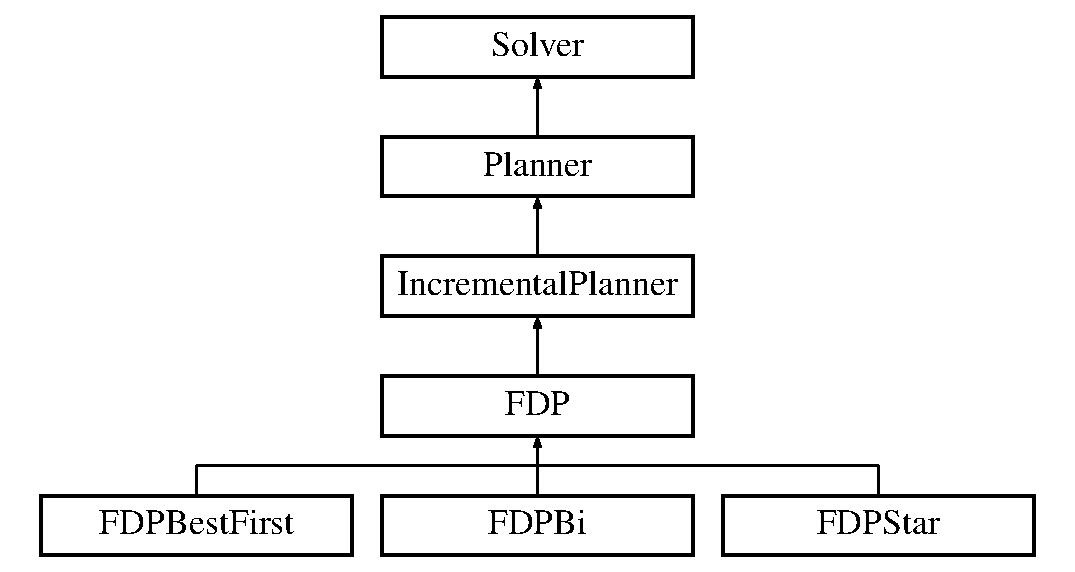
\includegraphics[height=5cm]{classFDP}
\end{center}
\end{figure}
\subsection*{Public Methods}
\begin{CompactItemize}
\item 
{\bf FDP} ({\bf Problem} $\ast$problem)
\begin{CompactList}\small\item\em A constructor that initializes data members.\item\end{CompactList}\item 
{\bf $\sim$FDP} ()
\begin{CompactList}\small\item\em Empty destructor.\item\end{CompactList}\item 
virtual void {\bf Reset} ()
\begin{CompactList}\small\item\em Reset the planner.\item\end{CompactList}\item 
virtual bool {\bf Plan} ()
\begin{CompactList}\small\item\em Attempt to solve an Initial-Goal query by growing an FDP tree.\item\end{CompactList}\end{CompactItemize}
\subsection*{Public Attributes}
\begin{CompactItemize}
\item 
int {\bf Satisfied\-Count}
\begin{CompactList}\small\item\em Number of times the collision checker has been called.\item\end{CompactList}\end{CompactItemize}
\subsection*{Protected Methods}
\begin{CompactItemize}
\item 
virtual double {\bf Search\-Cost} (double initcost, {\bf MSLNode} $\ast$\&n, {\bf MSLNode} $\ast$\&nn)
\item 
virtual vector$<$int$>$ {\bf State\-To\-Indices} (const {\bf MSLVector} \&x)
\item 
virtual {\bf MSLVector} {\bf Indices\-To\-State} (const vector$<$ int $>$ \&indices)
\end{CompactItemize}
\subsection*{Protected Attributes}
\begin{CompactItemize}
\item 
priority\_\-queue$<${\bf MSLNode}$\ast$,vector$<${\bf MSLNode}$\ast$$>$,{\bf MSLNode\-Greater}$>$ {\bf Q}
\begin{CompactList}\small\item\em Priority queue of nodes.\item\end{CompactList}\item 
{\bf Multi\-Array}$<$int$>$$\ast$ {\bf Grid}
\begin{CompactList}\small\item\em A quantized state space.\item\end{CompactList}\item 
vector$<$int$>$ {\bf Grid\-Dimensions}
\begin{CompactList}\small\item\em Dimensions for the grid.\item\end{CompactList}\item 
int {\bf Grid\-Default\-Resolution}
\begin{CompactList}\small\item\em Default size for each axis of the grid.\item\end{CompactList}\item 
{\bf MSLVector} {\bf Quantization}
\begin{CompactList}\small\item\em The quantized step size for each axis (computed automatically).\item\end{CompactList}\end{CompactItemize}


\subsection{Detailed Description}
A dynamic programming approach to nonholonomic planning, as proposed by Barraquand, Latombe, Algorithmica 10:6, pp. 121-155, 1993.

Forward Dynamic Programming, as proposed by Barraquand, Latombe,  Algorithmica 10:6, pp. 121-155, 1993. The solutions should be optimized  with respect to time, although problems can be caused by quantization  errors.

When an instance is constructed, a grid is initialized and each element of checked for collision. The test point for collision is the center of the cell. The current version does not use distance computations; therefore, a large value for Planner\-Delta\-T might cause collisions to be missed.

Make sure that Planner\-Delta\-T is large enough to allow the state to move from one cell to another without in a single step. For example, if the quantization leads to a grid boundary every 2.0 units, then Planner\-Delta\-T could be set to cause the state to change by 3.0 units.

Grid\-Dimensions sets the resolution of the grid and can be read from a file. For high-dimensional problems an error message may occur due to a grid that is too large. To enable larger grids, set the Max\-Size to a desirable size in the {\bf Multi\-Array} {\rm (p.\,\pageref{classMultiArray})} class (in {\bf marray.C}). 



\subsection{Constructor \& Destructor Documentation}
\index{FDP@{FDP}!FDP@{FDP}}
\index{FDP@{FDP}!FDP@{FDP}}
\subsubsection{\setlength{\rightskip}{0pt plus 5cm}FDP::FDP ({\bf Problem} $\ast$ {\em problem})}\label{classFDP_a0}


A constructor that initializes data members.

\index{FDP@{FDP}!~FDP@{$\sim$FDP}}
\index{~FDP@{$\sim$FDP}!FDP@{FDP}}
\subsubsection{\setlength{\rightskip}{0pt plus 5cm}FDP::$\sim$FDP ()\hspace{0.3cm}{\tt  [inline]}}\label{classFDP_a1}


Empty destructor.



\subsection{Member Function Documentation}
\index{FDP@{FDP}!IndicesToState@{IndicesToState}}
\index{IndicesToState@{IndicesToState}!FDP@{FDP}}
\subsubsection{\setlength{\rightskip}{0pt plus 5cm}{\bf MSLVector} FDP::Indices\-To\-State (const vector$<$ int $>$ \& {\em indices})\hspace{0.3cm}{\tt  [protected, virtual]}}\label{classFDP_b2}


\index{FDP@{FDP}!Plan@{Plan}}
\index{Plan@{Plan}!FDP@{FDP}}
\subsubsection{\setlength{\rightskip}{0pt plus 5cm}bool FDP::Plan ()\hspace{0.3cm}{\tt  [virtual]}}\label{classFDP_a3}


Attempt to solve an Initial-Goal query by growing an FDP tree.



Reimplemented from {\bf Planner} {\rm (p.\,\pageref{classPlanner_a4})}.

Reimplemented in {\bf FDPBi} {\rm (p.\,\pageref{classFDPBi_a3})}.\index{FDP@{FDP}!Reset@{Reset}}
\index{Reset@{Reset}!FDP@{FDP}}
\subsubsection{\setlength{\rightskip}{0pt plus 5cm}void FDP::Reset ()\hspace{0.3cm}{\tt  [virtual]}}\label{classFDP_a2}


Reset the planner.



Reimplemented from {\bf Planner} {\rm (p.\,\pageref{classPlanner_a2})}.

Reimplemented in {\bf FDPBi} {\rm (p.\,\pageref{classFDPBi_a2})}.\index{FDP@{FDP}!SearchCost@{SearchCost}}
\index{SearchCost@{SearchCost}!FDP@{FDP}}
\subsubsection{\setlength{\rightskip}{0pt plus 5cm}double FDP::Search\-Cost (double {\em initcost}, {\bf MSLNode} $\ast$\& {\em n}, {\bf MSLNode} $\ast$\& {\em nn})\hspace{0.3cm}{\tt  [protected, virtual]}}\label{classFDP_b0}




Reimplemented in {\bf FDPStar} {\rm (p.\,\pageref{classFDPStar_b0})}, and {\bf FDPBest\-First} {\rm (p.\,\pageref{classFDPBestFirst_b0})}.\index{FDP@{FDP}!StateToIndices@{StateToIndices}}
\index{StateToIndices@{StateToIndices}!FDP@{FDP}}
\subsubsection{\setlength{\rightskip}{0pt plus 5cm}vector$<$ int $>$ FDP::State\-To\-Indices$<$int$>$ (const {\bf MSLVector} \& {\em x})\hspace{0.3cm}{\tt  [protected, virtual]}}\label{classFDP_b1}




\subsection{Member Data Documentation}
\index{FDP@{FDP}!Grid@{Grid}}
\index{Grid@{Grid}!FDP@{FDP}}
\subsubsection{\setlength{\rightskip}{0pt plus 5cm}{\bf Multi\-Array}$<$ int $>$ $\ast$ FDP::Grid\hspace{0.3cm}{\tt  [protected]}}\label{classFDP_n1}


A quantized state space.

\index{FDP@{FDP}!GridDefaultResolution@{GridDefaultResolution}}
\index{GridDefaultResolution@{GridDefaultResolution}!FDP@{FDP}}
\subsubsection{\setlength{\rightskip}{0pt plus 5cm}int FDP::Grid\-Default\-Resolution\hspace{0.3cm}{\tt  [protected]}}\label{classFDP_n3}


Default size for each axis of the grid.

\index{FDP@{FDP}!GridDimensions@{GridDimensions}}
\index{GridDimensions@{GridDimensions}!FDP@{FDP}}
\subsubsection{\setlength{\rightskip}{0pt plus 5cm}vector$<$ int $>$ FDP::Grid\-Dimensions\hspace{0.3cm}{\tt  [protected]}}\label{classFDP_n2}


Dimensions for the grid.

\index{FDP@{FDP}!Q@{Q}}
\index{Q@{Q}!FDP@{FDP}}
\subsubsection{\setlength{\rightskip}{0pt plus 5cm}priority\_\-queue$<$ {\bf MSLNode} $\ast$,vector$<$ {\bf MSLNode} $\ast$$>$,{\bf MSLNode\-Greater} $>$ FDP::Q\hspace{0.3cm}{\tt  [protected]}}\label{classFDP_n0}


Priority queue of nodes.

\index{FDP@{FDP}!Quantization@{Quantization}}
\index{Quantization@{Quantization}!FDP@{FDP}}
\subsubsection{\setlength{\rightskip}{0pt plus 5cm}{\bf MSLVector} FDP::Quantization\hspace{0.3cm}{\tt  [protected]}}\label{classFDP_n4}


The quantized step size for each axis (computed automatically).

\index{FDP@{FDP}!SatisfiedCount@{SatisfiedCount}}
\index{SatisfiedCount@{SatisfiedCount}!FDP@{FDP}}
\subsubsection{\setlength{\rightskip}{0pt plus 5cm}int FDP::Satisfied\-Count}\label{classFDP_m0}


Number of times the collision checker has been called.



The documentation for this class was generated from the following files:\begin{CompactItemize}
\item 
{\bf fdp.h}\item 
{\bf fdp.C}\end{CompactItemize}

\section{FDPBest\-First  Class Reference}
\label{classFDPBestFirst}\index{FDPBestFirst@{FDPBest\-First}}
Best first search variant, using the Metric in {\bf Problem} {\rm (p.\,\pageref{classProblem})}. 


{\tt \#include $<$fdp.h$>$}

Inheritance diagram for FDPBest\-First::\begin{figure}[H]
\begin{center}
\leavevmode
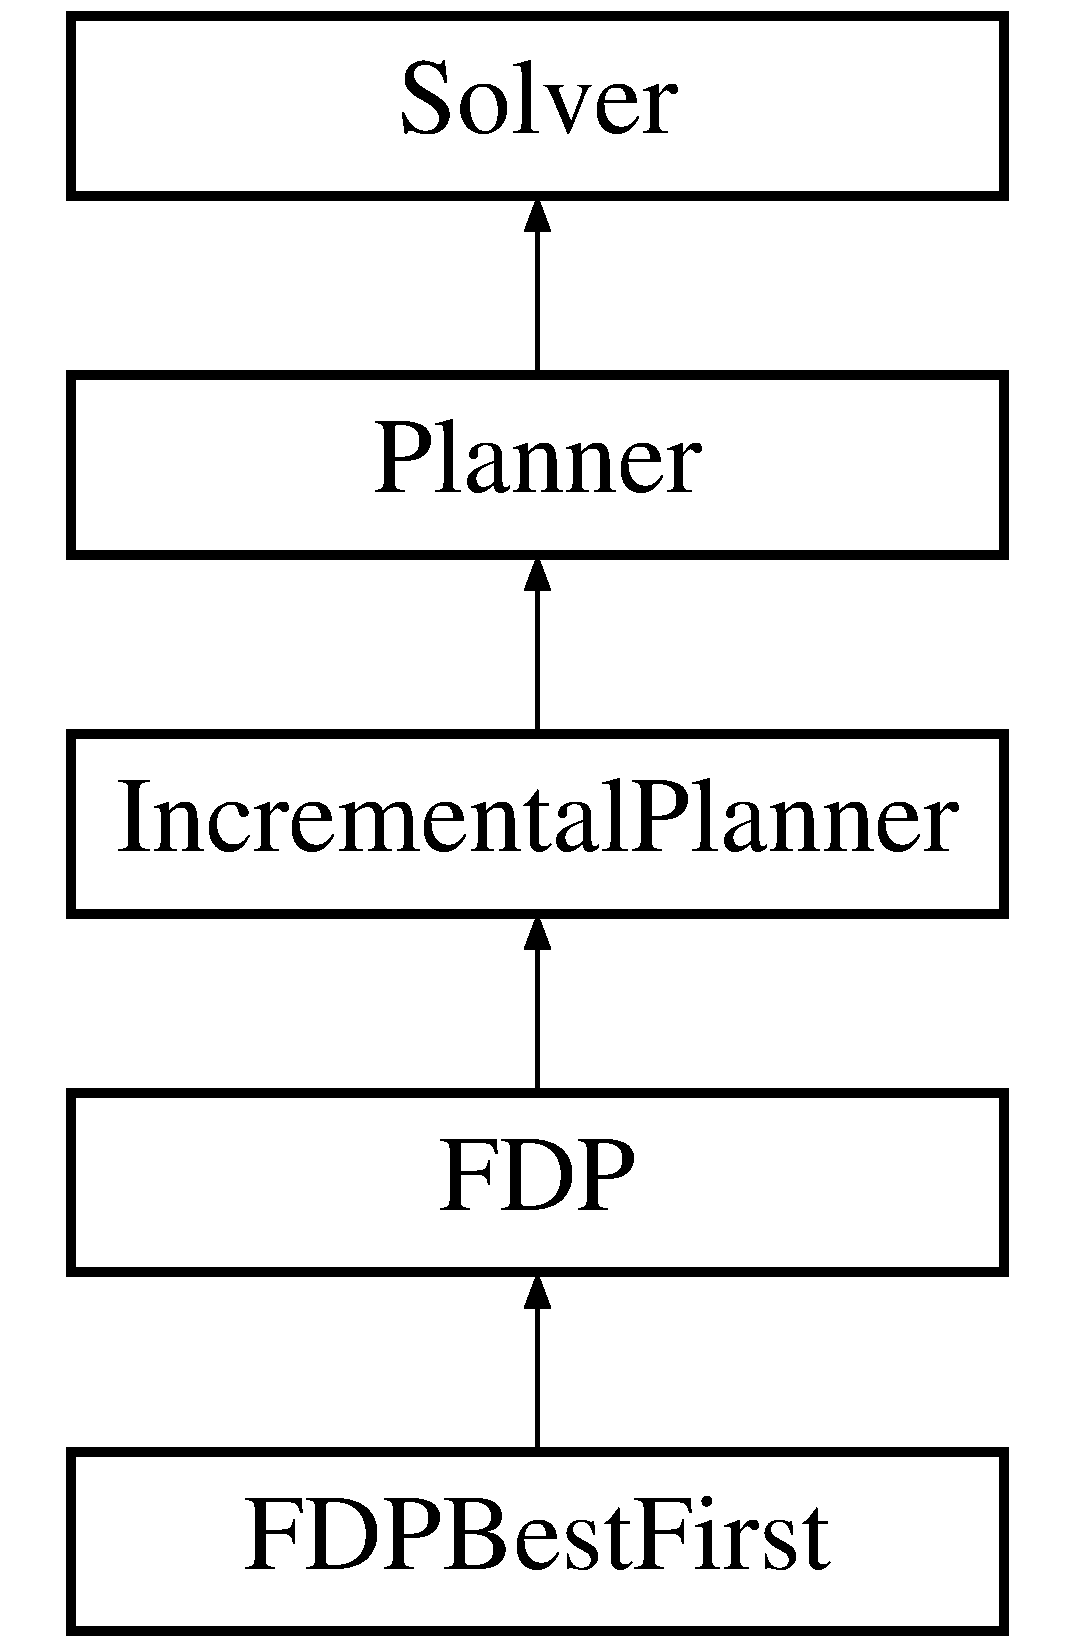
\includegraphics[height=5cm]{classFDPBestFirst}
\end{center}
\end{figure}
\subsection*{Public Methods}
\begin{CompactItemize}
\item 
{\bf FDPBest\-First} ({\bf Problem} $\ast$p)
\end{CompactItemize}
\subsection*{Protected Methods}
\begin{CompactItemize}
\item 
virtual double {\bf Search\-Cost} (double initcost, {\bf MSLNode} $\ast$\&n, {\bf MSLNode} $\ast$\&nn)
\end{CompactItemize}


\subsection{Detailed Description}
Best first search variant, using the Metric in {\bf Problem} {\rm (p.\,\pageref{classProblem})}.



\subsection{Constructor \& Destructor Documentation}
\index{FDPBestFirst@{FDPBest\-First}!FDPBestFirst@{FDPBestFirst}}
\index{FDPBestFirst@{FDPBestFirst}!FDPBestFirst@{FDPBest\-First}}
\subsubsection{\setlength{\rightskip}{0pt plus 5cm}FDPBest\-First::FDPBest\-First ({\bf Problem} $\ast$ {\em p})}\label{classFDPBestFirst_a0}




\subsection{Member Function Documentation}
\index{FDPBestFirst@{FDPBest\-First}!SearchCost@{SearchCost}}
\index{SearchCost@{SearchCost}!FDPBestFirst@{FDPBest\-First}}
\subsubsection{\setlength{\rightskip}{0pt plus 5cm}double FDPBest\-First::Search\-Cost (double {\em initcost}, {\bf MSLNode} $\ast$\& {\em n}, {\bf MSLNode} $\ast$\& {\em nn})\hspace{0.3cm}{\tt  [protected, virtual]}}\label{classFDPBestFirst_b0}




Reimplemented from {\bf FDP} {\rm (p.\,\pageref{classFDP_b0})}.

The documentation for this class was generated from the following files:\begin{CompactItemize}
\item 
{\bf fdp.h}\item 
{\bf fdp.C}\end{CompactItemize}

\section{FDPBi  Class Reference}
\label{classFDPBi}\index{FDPBi@{FDPBi}}
A bidirectional version of forward dynamic programming. 


{\tt \#include $<$fdp.h$>$}

Inheritance diagram for FDPBi::\begin{figure}[H]
\begin{center}
\leavevmode
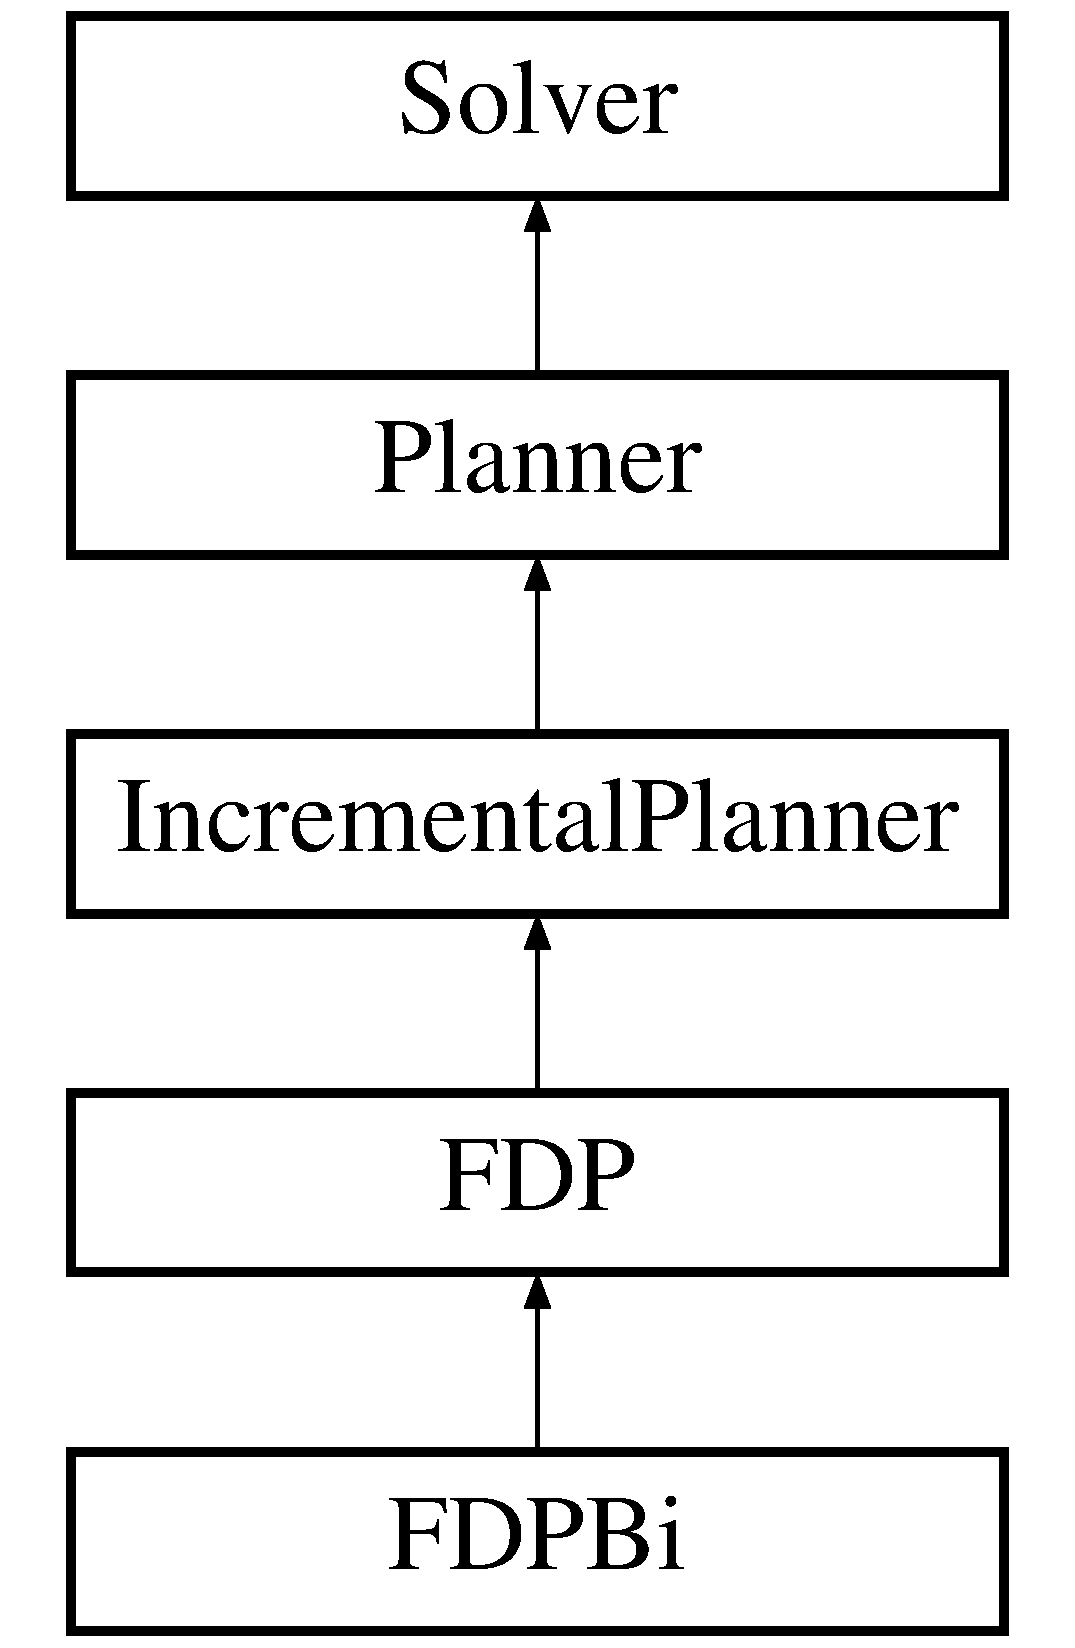
\includegraphics[height=5cm]{classFDPBi}
\end{center}
\end{figure}
\subsection*{Public Methods}
\begin{CompactItemize}
\item 
{\bf FDPBi} ({\bf Problem} $\ast$problem)
\begin{CompactList}\small\item\em A constructor that initializes data members.\item\end{CompactList}\item 
{\bf $\sim$FDPBi} ()
\begin{CompactList}\small\item\em Empty destructor.\item\end{CompactList}\item 
virtual void {\bf Reset} ()
\begin{CompactList}\small\item\em Reset the planner.\item\end{CompactList}\item 
virtual bool {\bf Plan} ()
\begin{CompactList}\small\item\em Attempt to solve an Initial-Goal query by growing an {\bf FDP} {\rm (p.\,\pageref{classFDP})}.\item\end{CompactList}\end{CompactItemize}
\subsection*{Protected Methods}
\begin{CompactItemize}
\item 
void {\bf Recover\-Solution} ({\bf MSLNode} $\ast$\&n1, {\bf MSLNode} $\ast$\&n2)
\begin{CompactList}\small\item\em Pull out the path and timings from the graphs.\item\end{CompactList}\end{CompactItemize}
\subsection*{Protected Attributes}
\begin{CompactItemize}
\item 
priority\_\-queue$<${\bf MSLNode}$\ast$,vector$<${\bf MSLNode}$\ast$$>$,{\bf MSLNode\-Greater}$>$ {\bf Q2}
\begin{CompactList}\small\item\em Priority queue of nodes.\item\end{CompactList}\end{CompactItemize}


\subsection{Detailed Description}
A bidirectional version of forward dynamic programming.



\subsection{Constructor \& Destructor Documentation}
\index{FDPBi@{FDPBi}!FDPBi@{FDPBi}}
\index{FDPBi@{FDPBi}!FDPBi@{FDPBi}}
\subsubsection{\setlength{\rightskip}{0pt plus 5cm}FDPBi::FDPBi ({\bf Problem} $\ast$ {\em problem})}\label{classFDPBi_a0}


A constructor that initializes data members.

\index{FDPBi@{FDPBi}!~FDPBi@{$\sim$FDPBi}}
\index{~FDPBi@{$\sim$FDPBi}!FDPBi@{FDPBi}}
\subsubsection{\setlength{\rightskip}{0pt plus 5cm}FDPBi::$\sim$FDPBi ()\hspace{0.3cm}{\tt  [inline]}}\label{classFDPBi_a1}


Empty destructor.



\subsection{Member Function Documentation}
\index{FDPBi@{FDPBi}!Plan@{Plan}}
\index{Plan@{Plan}!FDPBi@{FDPBi}}
\subsubsection{\setlength{\rightskip}{0pt plus 5cm}bool FDPBi::Plan ()\hspace{0.3cm}{\tt  [virtual]}}\label{classFDPBi_a3}


Attempt to solve an Initial-Goal query by growing an {\bf FDP} {\rm (p.\,\pageref{classFDP})}.



Reimplemented from {\bf FDP} {\rm (p.\,\pageref{classFDP_a3})}.\index{FDPBi@{FDPBi}!RecoverSolution@{RecoverSolution}}
\index{RecoverSolution@{RecoverSolution}!FDPBi@{FDPBi}}
\subsubsection{\setlength{\rightskip}{0pt plus 5cm}void FDPBi::Recover\-Solution ({\bf MSLNode} $\ast$\& {\em n1}, {\bf MSLNode} $\ast$\& {\em n2})\hspace{0.3cm}{\tt  [protected]}}\label{classFDPBi_b0}


Pull out the path and timings from the graphs.

\index{FDPBi@{FDPBi}!Reset@{Reset}}
\index{Reset@{Reset}!FDPBi@{FDPBi}}
\subsubsection{\setlength{\rightskip}{0pt plus 5cm}void FDPBi::Reset ()\hspace{0.3cm}{\tt  [virtual]}}\label{classFDPBi_a2}


Reset the planner.



Reimplemented from {\bf FDP} {\rm (p.\,\pageref{classFDP_a2})}.

\subsection{Member Data Documentation}
\index{FDPBi@{FDPBi}!Q2@{Q2}}
\index{Q2@{Q2}!FDPBi@{FDPBi}}
\subsubsection{\setlength{\rightskip}{0pt plus 5cm}priority\_\-queue$<$ {\bf MSLNode} $\ast$,vector$<$ {\bf MSLNode} $\ast$$>$,{\bf MSLNode\-Greater} $>$ FDPBi::Q2\hspace{0.3cm}{\tt  [protected]}}\label{classFDPBi_n0}


Priority queue of nodes.



The documentation for this class was generated from the following files:\begin{CompactItemize}
\item 
{\bf fdp.h}\item 
{\bf fdp.C}\end{CompactItemize}

\section{FDPStar  Class Reference}
\label{classFDPStar}\index{FDPStar@{FDPStar}}
An A-Star search variant. The Metric in {\bf Problem} {\rm (p.\,\pageref{classProblem})} is used as the cost. 


{\tt \#include $<$fdp.h$>$}

Inheritance diagram for FDPStar::\begin{figure}[H]
\begin{center}
\leavevmode
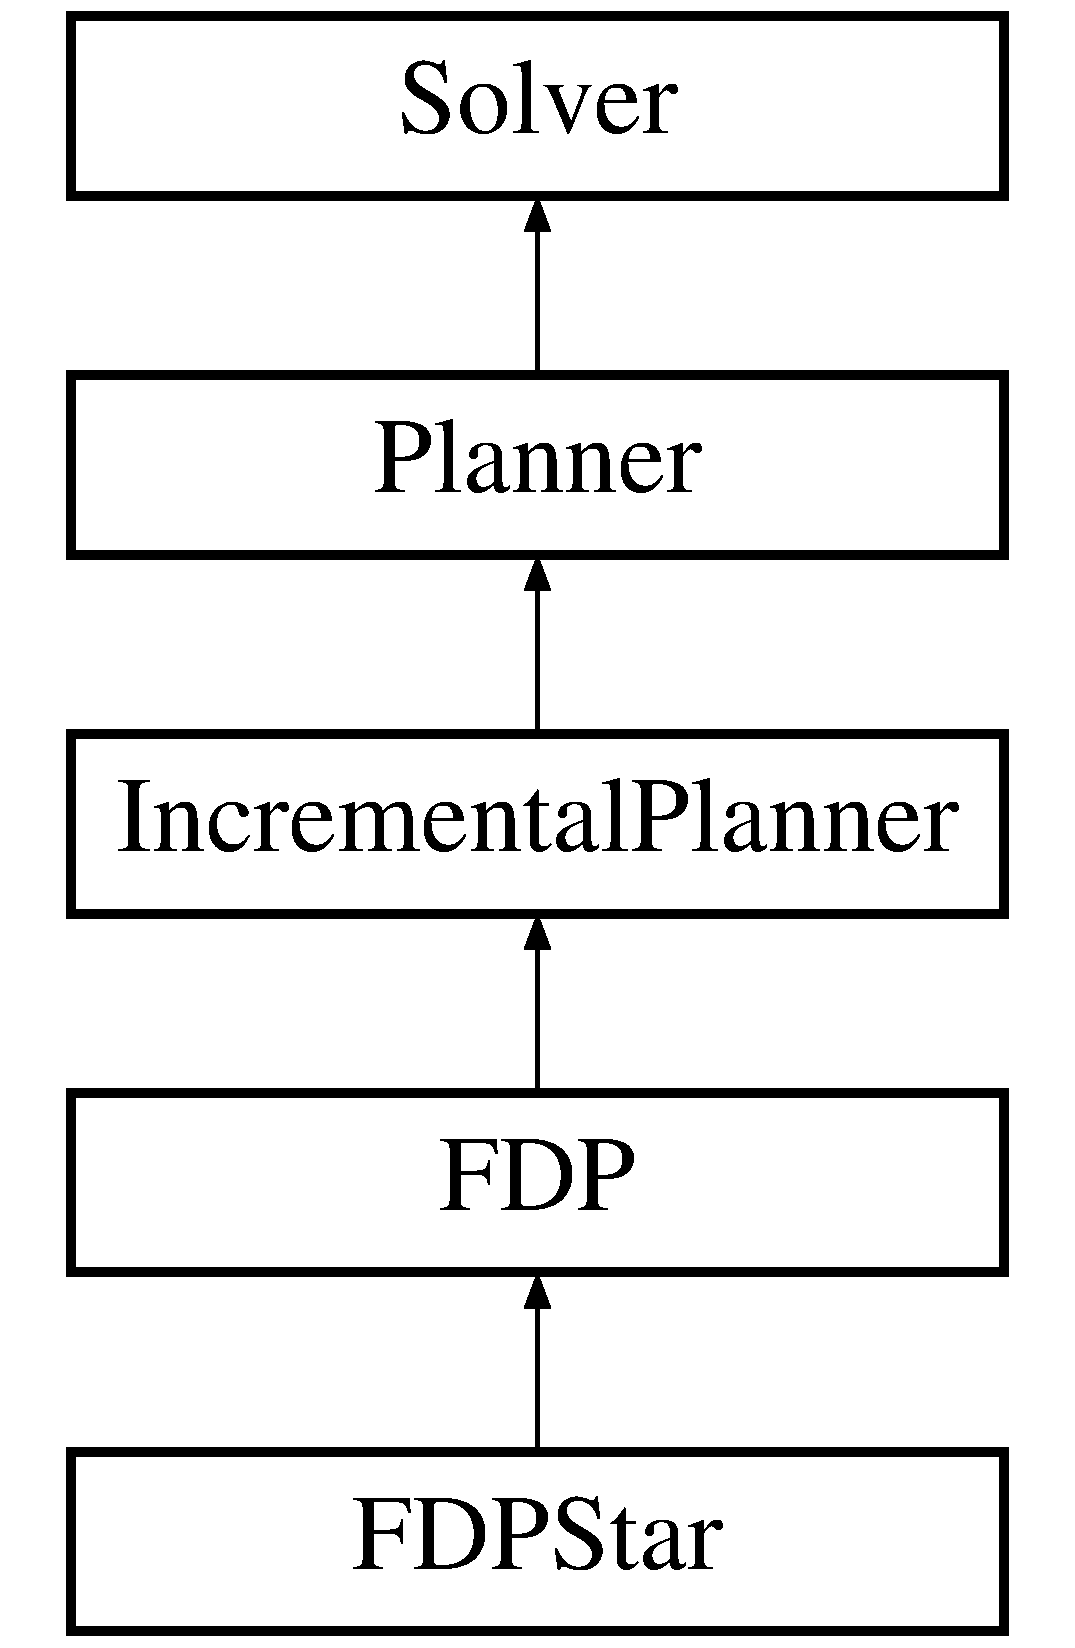
\includegraphics[height=5cm]{classFDPStar}
\end{center}
\end{figure}
\subsection*{Public Methods}
\begin{CompactItemize}
\item 
{\bf FDPStar} ({\bf Problem} $\ast$p)
\end{CompactItemize}
\subsection*{Protected Methods}
\begin{CompactItemize}
\item 
virtual double {\bf Search\-Cost} (double initcost, {\bf MSLNode} $\ast$\&n, {\bf MSLNode} $\ast$\&nn)
\end{CompactItemize}


\subsection{Detailed Description}
An A-Star search variant. The Metric in {\bf Problem} {\rm (p.\,\pageref{classProblem})} is used as the cost.



\subsection{Constructor \& Destructor Documentation}
\index{FDPStar@{FDPStar}!FDPStar@{FDPStar}}
\index{FDPStar@{FDPStar}!FDPStar@{FDPStar}}
\subsubsection{\setlength{\rightskip}{0pt plus 5cm}FDPStar::FDPStar ({\bf Problem} $\ast$ {\em p})}\label{classFDPStar_a0}




\subsection{Member Function Documentation}
\index{FDPStar@{FDPStar}!SearchCost@{SearchCost}}
\index{SearchCost@{SearchCost}!FDPStar@{FDPStar}}
\subsubsection{\setlength{\rightskip}{0pt plus 5cm}double FDPStar::Search\-Cost (double {\em initcost}, {\bf MSLNode} $\ast$\& {\em n}, {\bf MSLNode} $\ast$\& {\em nn})\hspace{0.3cm}{\tt  [protected, virtual]}}\label{classFDPStar_b0}




Reimplemented from {\bf FDP} {\rm (p.\,\pageref{classFDP_b0})}.

The documentation for this class was generated from the following files:\begin{CompactItemize}
\item 
{\bf fdp.h}\item 
{\bf fdp.C}\end{CompactItemize}

\section{FXApp  Class Reference}
\label{classFXApp}\index{FXApp@{FXApp}}
Inheritance diagram for FXApp::\begin{figure}[H]
\begin{center}
\leavevmode
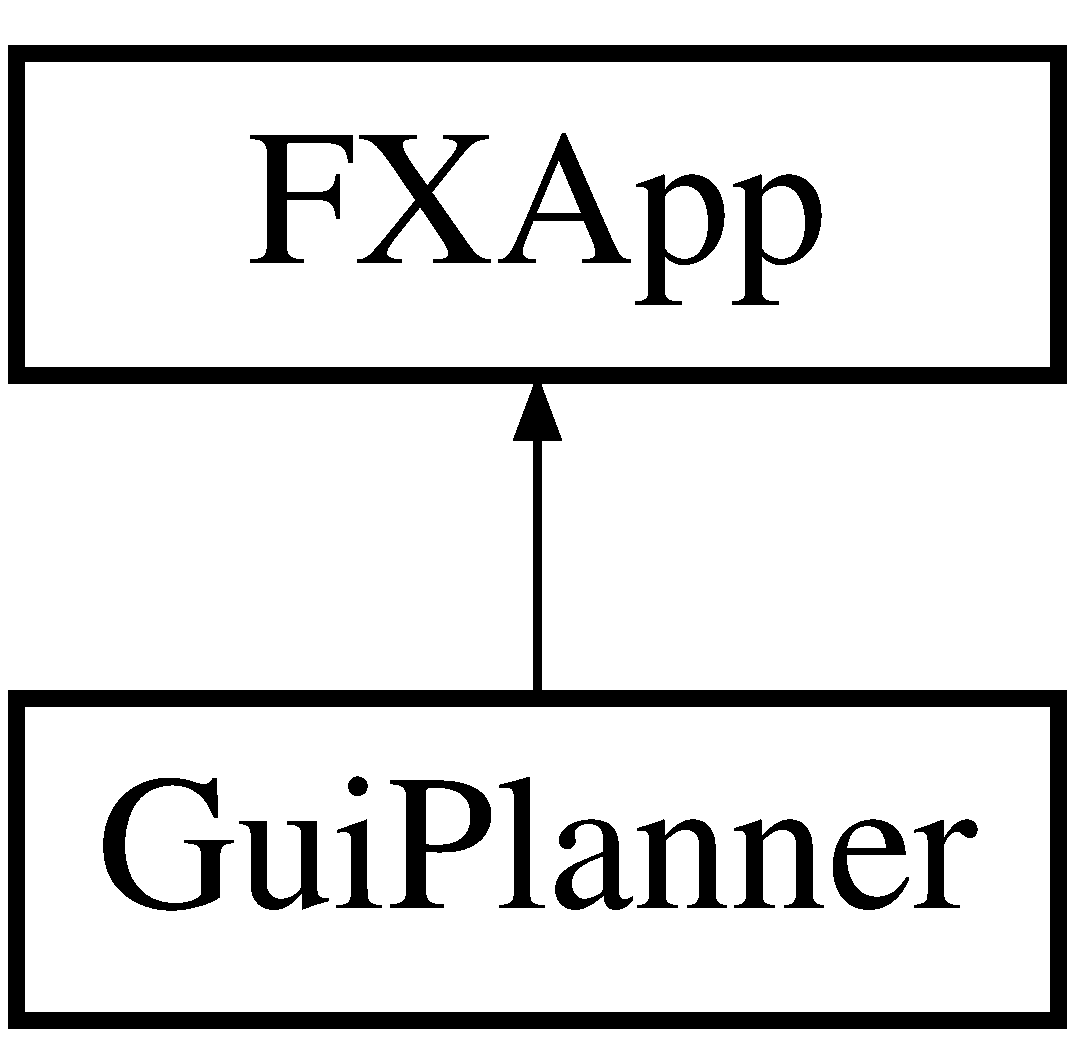
\includegraphics[height=2cm]{classFXApp}
\end{center}
\end{figure}


The documentation for this class was generated from the following file:\begin{CompactItemize}
\item 
{\bf guiplanner.h}\end{CompactItemize}

\section{FXDialog\-Box  Class Reference}
\label{classFXDialogBox}\index{FXDialogBox@{FXDialog\-Box}}
Inheritance diagram for FXDialog\-Box::\begin{figure}[H]
\begin{center}
\leavevmode
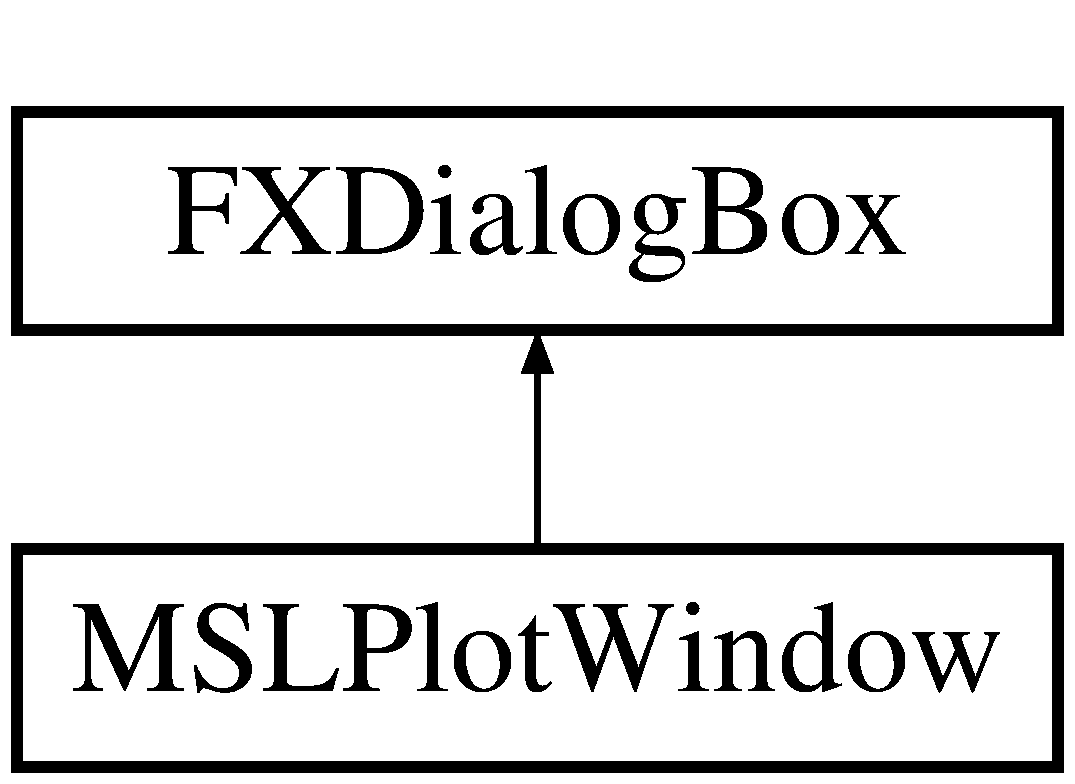
\includegraphics[height=2cm]{classFXDialogBox}
\end{center}
\end{figure}


The documentation for this class was generated from the following file:\begin{CompactItemize}
\item 
{\bf guiplanner.h}\end{CompactItemize}

\section{FXMain\-Window  Class Reference}
\label{classFXMainWindow}\index{FXMainWindow@{FXMain\-Window}}
Inheritance diagram for FXMain\-Window::\begin{figure}[H]
\begin{center}
\leavevmode
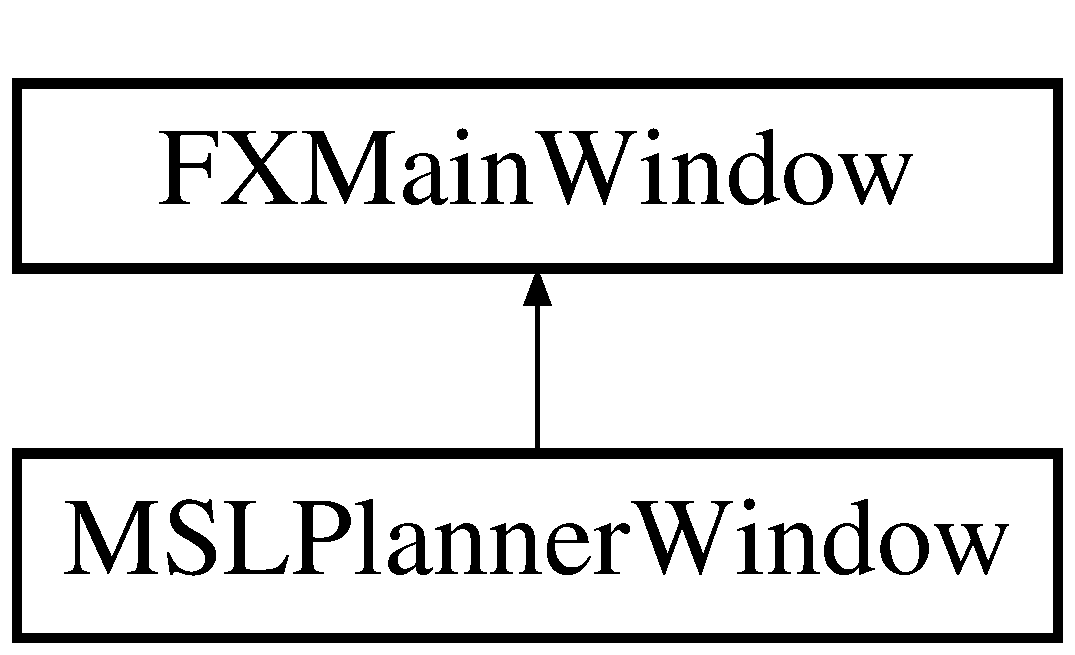
\includegraphics[height=2cm]{classFXMainWindow}
\end{center}
\end{figure}


The documentation for this class was generated from the following file:\begin{CompactItemize}
\item 
{\bf guiplanner.h}\end{CompactItemize}

\section{Geom  Class Reference}
\label{classGeom}\index{Geom@{Geom}}
Geometric models and collision detection methods. 


{\tt \#include $<$geom.h$>$}

Inheritance diagram for Geom::\begin{figure}[H]
\begin{center}
\leavevmode
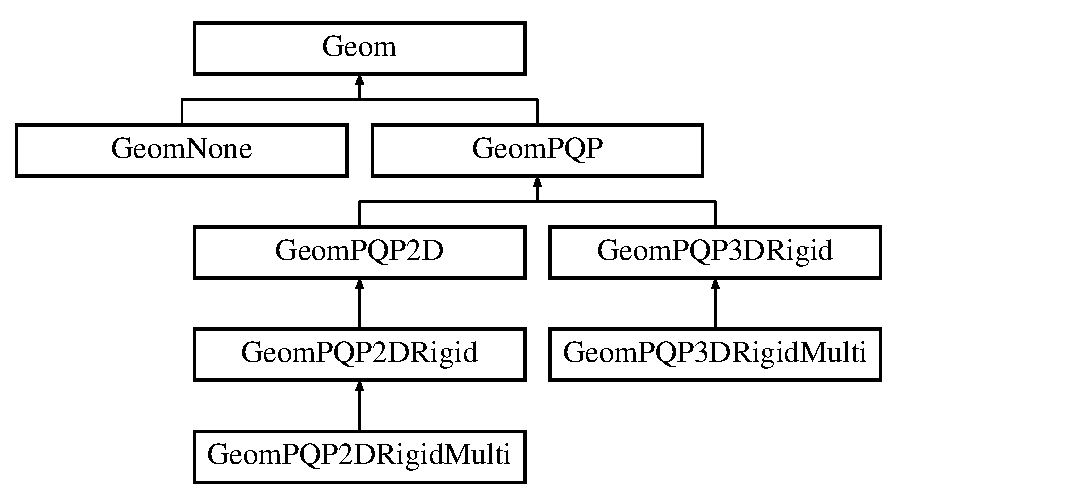
\includegraphics[height=5cm]{classGeom}
\end{center}
\end{figure}
\subsection*{Public Methods}
\begin{CompactItemize}
\item 
{\bf Geom} (string path)
\begin{CompactList}\small\item\em Empty constructor in base class.\item\end{CompactList}\item 
virtual {\bf $\sim$Geom} ()
\begin{CompactList}\small\item\em Empty destructor.\item\end{CompactList}\item 
virtual bool {\bf Collision\-Free} (const {\bf MSLVector} \&q)=0
\begin{CompactList}\small\item\em Return true if the robot(s) and obstacles are not in collision.\item\end{CompactList}\item 
virtual double {\bf Distance\-Comp} (const {\bf MSLVector} \&q)=0
\begin{CompactList}\small\item\em Compute the distance of the closest point on the robot to the obstacle region.\item\end{CompactList}\item 
virtual {\bf MSLVector} {\bf Configuration\-Difference} (const {\bf MSLVector} \&q1, const {\bf MSLVector} \&q2)
\begin{CompactList}\small\item\em Compute a {\bf MSLVector} {\rm (p.\,\pageref{classMSLVector})} based on q2-q1. In R$^\wedge$n, the configurations are simply subtracted to make the {\bf MSLVector} {\rm (p.\,\pageref{classMSLVector})}. This method exists to make things work correctly for other configuration-space topologies.\item\end{CompactList}\end{CompactItemize}
\subsection*{Public Attributes}
\begin{CompactItemize}
\item 
int {\bf Num\-Bodies}
\begin{CompactList}\small\item\em The number of rigid bodies in the geometry model.\item\end{CompactList}\item 
int {\bf Geom\-Dim}
\begin{CompactList}\small\item\em The dimension of the world geometry: 2 or 3.\item\end{CompactList}\item 
{\bf MSLVector} {\bf Max\-Deviates}
\begin{CompactList}\small\item\em Maximum displacement of geometry with respect to change in each variable.\item\end{CompactList}\end{CompactItemize}
\subsection*{Protected Attributes}
\begin{CompactItemize}
\item 
string {\bf File\-Path}
\end{CompactItemize}


\subsection{Detailed Description}
Geometric models and collision detection methods.

These classes define the geometric representations of all obstacles in the world, and of each part of the robot. The methods allow planning algorithms to determine whether any of the robot parts are in collision with each other or with obstacles in the world.

A configuration vector specifies the positions and orientation of each rigid body. 



\subsection{Constructor \& Destructor Documentation}
\index{Geom@{Geom}!Geom@{Geom}}
\index{Geom@{Geom}!Geom@{Geom}}
\subsubsection{\setlength{\rightskip}{0pt plus 5cm}Geom::Geom (string {\em path} = \char`\"{}\char`\"{})}\label{classGeom_a0}


Empty constructor in base class.

\index{Geom@{Geom}!~Geom@{$\sim$Geom}}
\index{~Geom@{$\sim$Geom}!Geom@{Geom}}
\subsubsection{\setlength{\rightskip}{0pt plus 5cm}Geom::$\sim$Geom ()\hspace{0.3cm}{\tt  [inline, virtual]}}\label{classGeom_a1}


Empty destructor.



\subsection{Member Function Documentation}
\index{Geom@{Geom}!CollisionFree@{CollisionFree}}
\index{CollisionFree@{CollisionFree}!Geom@{Geom}}
\subsubsection{\setlength{\rightskip}{0pt plus 5cm}bool Geom::Collision\-Free (const {\bf MSLVector} \& {\em q})\hspace{0.3cm}{\tt  [pure virtual]}}\label{classGeom_a2}


Return true if the robot(s) and obstacles are not in collision.



Reimplemented in {\bf Geom\-None} {\rm (p.\,\pageref{classGeomNone_a2})}, {\bf Geom\-PQP} {\rm (p.\,\pageref{classGeomPQP_a4})}, {\bf Geom\-PQP2DRigid} {\rm (p.\,\pageref{classGeomPQP2DRigid_a2})}, {\bf Geom\-PQP2DRigid\-Multi} {\rm (p.\,\pageref{classGeomPQP2DRigidMulti_a2})}, {\bf Geom\-PQP3DRigid} {\rm (p.\,\pageref{classGeomPQP3DRigid_a2})}, and {\bf Geom\-PQP3DRigid\-Multi} {\rm (p.\,\pageref{classGeomPQP3DRigidMulti_a2})}.\index{Geom@{Geom}!ConfigurationDifference@{ConfigurationDifference}}
\index{ConfigurationDifference@{ConfigurationDifference}!Geom@{Geom}}
\subsubsection{\setlength{\rightskip}{0pt plus 5cm}{\bf MSLVector} Geom::Configuration\-Difference (const {\bf MSLVector} \& {\em q1}, const {\bf MSLVector} \& {\em q2})\hspace{0.3cm}{\tt  [virtual]}}\label{classGeom_a4}


Compute a {\bf MSLVector} {\rm (p.\,\pageref{classMSLVector})} based on q2-q1. In R$^\wedge$n, the configurations are simply subtracted to make the {\bf MSLVector} {\rm (p.\,\pageref{classMSLVector})}. This method exists to make things work correctly for other configuration-space topologies.



Reimplemented in {\bf Geom\-PQP2DRigid} {\rm (p.\,\pageref{classGeomPQP2DRigid_a4})}, and {\bf Geom\-PQP3DRigid} {\rm (p.\,\pageref{classGeomPQP3DRigid_a4})}.\index{Geom@{Geom}!DistanceComp@{DistanceComp}}
\index{DistanceComp@{DistanceComp}!Geom@{Geom}}
\subsubsection{\setlength{\rightskip}{0pt plus 5cm}double Geom::Distance\-Comp (const {\bf MSLVector} \& {\em q})\hspace{0.3cm}{\tt  [pure virtual]}}\label{classGeom_a3}


Compute the distance of the closest point on the robot to the obstacle region.



Reimplemented in {\bf Geom\-None} {\rm (p.\,\pageref{classGeomNone_a3})}, {\bf Geom\-PQP} {\rm (p.\,\pageref{classGeomPQP_a5})}, {\bf Geom\-PQP2DRigid} {\rm (p.\,\pageref{classGeomPQP2DRigid_a3})}, {\bf Geom\-PQP2DRigid\-Multi} {\rm (p.\,\pageref{classGeomPQP2DRigidMulti_a3})}, {\bf Geom\-PQP3DRigid} {\rm (p.\,\pageref{classGeomPQP3DRigid_a3})}, and {\bf Geom\-PQP3DRigid\-Multi} {\rm (p.\,\pageref{classGeomPQP3DRigidMulti_a3})}.

\subsection{Member Data Documentation}
\index{Geom@{Geom}!FilePath@{FilePath}}
\index{FilePath@{FilePath}!Geom@{Geom}}
\subsubsection{\setlength{\rightskip}{0pt plus 5cm}string Geom::File\-Path\hspace{0.3cm}{\tt  [protected]}}\label{classGeom_n0}


\index{Geom@{Geom}!GeomDim@{GeomDim}}
\index{GeomDim@{GeomDim}!Geom@{Geom}}
\subsubsection{\setlength{\rightskip}{0pt plus 5cm}int Geom::Geom\-Dim}\label{classGeom_m1}


The dimension of the world geometry: 2 or 3.

\index{Geom@{Geom}!MaxDeviates@{MaxDeviates}}
\index{MaxDeviates@{MaxDeviates}!Geom@{Geom}}
\subsubsection{\setlength{\rightskip}{0pt plus 5cm}{\bf MSLVector} Geom::Max\-Deviates}\label{classGeom_m2}


Maximum displacement of geometry with respect to change in each variable.

\index{Geom@{Geom}!NumBodies@{NumBodies}}
\index{NumBodies@{NumBodies}!Geom@{Geom}}
\subsubsection{\setlength{\rightskip}{0pt plus 5cm}int Geom::Num\-Bodies}\label{classGeom_m0}


The number of rigid bodies in the geometry model.



The documentation for this class was generated from the following files:\begin{CompactItemize}
\item 
{\bf geom.h}\item 
{\bf geom.C}\end{CompactItemize}

\section{Geom\-None  Class Reference}
\label{classGeomNone}\index{GeomNone@{Geom\-None}}
A class with no geometry -- a collision never happens. 


{\tt \#include $<$geom.h$>$}

Inheritance diagram for Geom\-None::\begin{figure}[H]
\begin{center}
\leavevmode
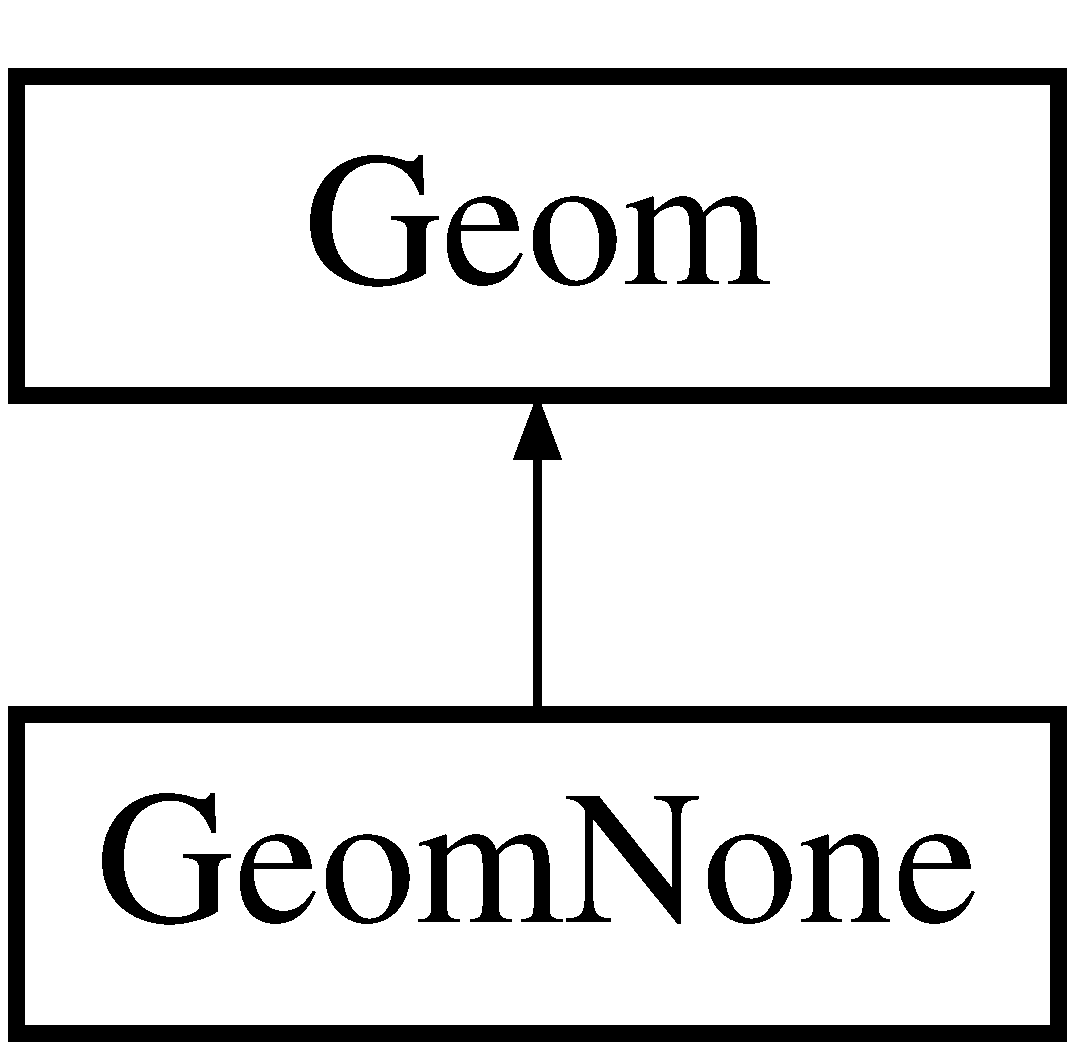
\includegraphics[height=2cm]{classGeomNone}
\end{center}
\end{figure}
\subsection*{Public Methods}
\begin{CompactItemize}
\item 
{\bf Geom\-None} (string path)
\item 
virtual {\bf $\sim$Geom\-None} ()
\item 
virtual bool {\bf Collision\-Free} (const {\bf MSLVector} \&q)
\begin{CompactList}\small\item\em Return true if the robot(s) and obstacles are not in collision.\item\end{CompactList}\item 
virtual double {\bf Distance\-Comp} (const {\bf MSLVector} \&q)
\begin{CompactList}\small\item\em Compute the distance of the closest point on the robot to the obstacle region.\item\end{CompactList}\end{CompactItemize}


\subsection{Detailed Description}
A class with no geometry -- a collision never happens.



\subsection{Constructor \& Destructor Documentation}
\index{GeomNone@{Geom\-None}!GeomNone@{GeomNone}}
\index{GeomNone@{GeomNone}!GeomNone@{Geom\-None}}
\subsubsection{\setlength{\rightskip}{0pt plus 5cm}Geom\-None::Geom\-None (string {\em path} = \char`\"{}\char`\"{})}\label{classGeomNone_a0}


\index{GeomNone@{Geom\-None}!~GeomNone@{$\sim$GeomNone}}
\index{~GeomNone@{$\sim$GeomNone}!GeomNone@{Geom\-None}}
\subsubsection{\setlength{\rightskip}{0pt plus 5cm}Geom\-None::$\sim$Geom\-None ()\hspace{0.3cm}{\tt  [inline, virtual]}}\label{classGeomNone_a1}




\subsection{Member Function Documentation}
\index{GeomNone@{Geom\-None}!CollisionFree@{CollisionFree}}
\index{CollisionFree@{CollisionFree}!GeomNone@{Geom\-None}}
\subsubsection{\setlength{\rightskip}{0pt plus 5cm}bool Geom\-None::Collision\-Free (const {\bf MSLVector} \& {\em q})\hspace{0.3cm}{\tt  [inline, virtual]}}\label{classGeomNone_a2}


Return true if the robot(s) and obstacles are not in collision.



Reimplemented from {\bf Geom} {\rm (p.\,\pageref{classGeom_a2})}.\index{GeomNone@{Geom\-None}!DistanceComp@{DistanceComp}}
\index{DistanceComp@{DistanceComp}!GeomNone@{Geom\-None}}
\subsubsection{\setlength{\rightskip}{0pt plus 5cm}double Geom\-None::Distance\-Comp (const {\bf MSLVector} \& {\em q})\hspace{0.3cm}{\tt  [inline, virtual]}}\label{classGeomNone_a3}


Compute the distance of the closest point on the robot to the obstacle region.



Reimplemented from {\bf Geom} {\rm (p.\,\pageref{classGeom_a3})}.

The documentation for this class was generated from the following files:\begin{CompactItemize}
\item 
{\bf geom.h}\item 
{\bf geom.C}\end{CompactItemize}

\section{Geom\-PQP  Class Reference}
\label{classGeomPQP}\index{GeomPQP@{Geom\-PQP}}
Parent class PQP-based {\bf list} {\rm (p.\,\pageref{classlist})} of Triangle models. 


{\tt \#include $<$geom\-PQP.h$>$}

Inheritance diagram for Geom\-PQP::\begin{figure}[H]
\begin{center}
\leavevmode
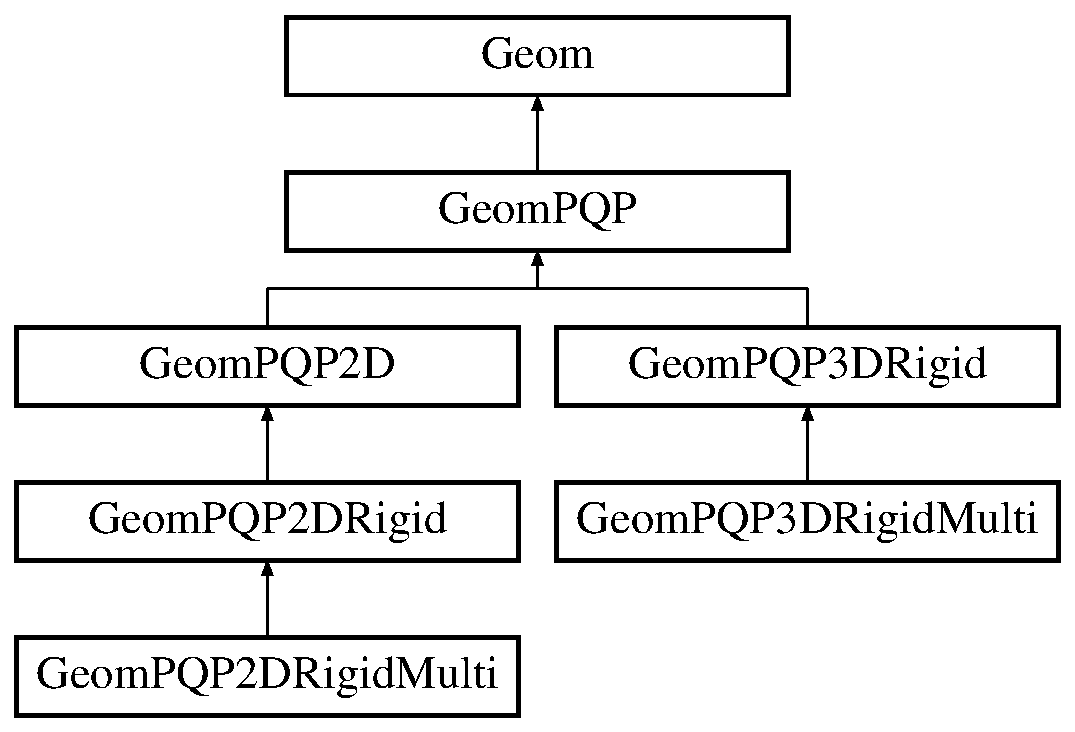
\includegraphics[height=5cm]{classGeomPQP}
\end{center}
\end{figure}
\subsection*{Public Methods}
\begin{CompactItemize}
\item 
{\bf Geom\-PQP} (string path)
\item 
virtual {\bf $\sim$Geom\-PQP} ()
\item 
virtual void {\bf Load\-Environment} (string path)
\item 
virtual void {\bf Load\-Robot} (string path)
\item 
virtual bool {\bf Collision\-Free} (const {\bf MSLVector} \&q)
\begin{CompactList}\small\item\em Return true if the robot(s) and obstacles are not in collision.\item\end{CompactList}\item 
virtual double {\bf Distance\-Comp} (const {\bf MSLVector} \&q)
\begin{CompactList}\small\item\em Compute the distance of the closest point on the robot to the obstacle region.\item\end{CompactList}\end{CompactItemize}
\subsection*{Public Attributes}
\begin{CompactItemize}
\item 
{\bf list}$<${\bf MSLTriangle}$>$ {\bf Obst}
\item 
{\bf list}$<${\bf MSLTriangle}$>$ {\bf Robot}
\item 
PQP\_\-Model {\bf Ro}
\item 
PQP\_\-Model {\bf Ob}
\end{CompactItemize}
\subsection*{Protected Attributes}
\begin{CompactItemize}
\item 
PQP\_\-REAL {\bf RR} [3][3]
\item 
PQP\_\-REAL {\bf RO} [3][3]
\item 
PQP\_\-REAL {\bf TR} [3]
\item 
PQP\_\-REAL {\bf TO} [3]
\end{CompactItemize}


\subsection{Detailed Description}
Parent class PQP-based {\bf list} {\rm (p.\,\pageref{classlist})} of Triangle models.



\subsection{Constructor \& Destructor Documentation}
\index{GeomPQP@{Geom\-PQP}!GeomPQP@{GeomPQP}}
\index{GeomPQP@{GeomPQP}!GeomPQP@{Geom\-PQP}}
\subsubsection{\setlength{\rightskip}{0pt plus 5cm}Geom\-PQP::Geom\-PQP (string {\em path} = \char`\"{}\char`\"{})}\label{classGeomPQP_a0}


\index{GeomPQP@{Geom\-PQP}!~GeomPQP@{$\sim$GeomPQP}}
\index{~GeomPQP@{$\sim$GeomPQP}!GeomPQP@{Geom\-PQP}}
\subsubsection{\setlength{\rightskip}{0pt plus 5cm}Geom\-PQP::$\sim$Geom\-PQP ()\hspace{0.3cm}{\tt  [inline, virtual]}}\label{classGeomPQP_a1}




\subsection{Member Function Documentation}
\index{GeomPQP@{Geom\-PQP}!CollisionFree@{CollisionFree}}
\index{CollisionFree@{CollisionFree}!GeomPQP@{Geom\-PQP}}
\subsubsection{\setlength{\rightskip}{0pt plus 5cm}bool Geom\-PQP::Collision\-Free (const {\bf MSLVector} \& {\em q})\hspace{0.3cm}{\tt  [inline, virtual]}}\label{classGeomPQP_a4}


Return true if the robot(s) and obstacles are not in collision.



Reimplemented from {\bf Geom} {\rm (p.\,\pageref{classGeom_a2})}.

Reimplemented in {\bf Geom\-PQP2DRigid} {\rm (p.\,\pageref{classGeomPQP2DRigid_a2})}, {\bf Geom\-PQP2DRigid\-Multi} {\rm (p.\,\pageref{classGeomPQP2DRigidMulti_a2})}, {\bf Geom\-PQP3DRigid} {\rm (p.\,\pageref{classGeomPQP3DRigid_a2})}, and {\bf Geom\-PQP3DRigid\-Multi} {\rm (p.\,\pageref{classGeomPQP3DRigidMulti_a2})}.\index{GeomPQP@{Geom\-PQP}!DistanceComp@{DistanceComp}}
\index{DistanceComp@{DistanceComp}!GeomPQP@{Geom\-PQP}}
\subsubsection{\setlength{\rightskip}{0pt plus 5cm}double Geom\-PQP::Distance\-Comp (const {\bf MSLVector} \& {\em q})\hspace{0.3cm}{\tt  [inline, virtual]}}\label{classGeomPQP_a5}


Compute the distance of the closest point on the robot to the obstacle region.



Reimplemented from {\bf Geom} {\rm (p.\,\pageref{classGeom_a3})}.

Reimplemented in {\bf Geom\-PQP2DRigid} {\rm (p.\,\pageref{classGeomPQP2DRigid_a3})}, {\bf Geom\-PQP2DRigid\-Multi} {\rm (p.\,\pageref{classGeomPQP2DRigidMulti_a3})}, {\bf Geom\-PQP3DRigid} {\rm (p.\,\pageref{classGeomPQP3DRigid_a3})}, and {\bf Geom\-PQP3DRigid\-Multi} {\rm (p.\,\pageref{classGeomPQP3DRigidMulti_a3})}.\index{GeomPQP@{Geom\-PQP}!LoadEnvironment@{LoadEnvironment}}
\index{LoadEnvironment@{LoadEnvironment}!GeomPQP@{Geom\-PQP}}
\subsubsection{\setlength{\rightskip}{0pt plus 5cm}void Geom\-PQP::Load\-Environment (string {\em path})\hspace{0.3cm}{\tt  [virtual]}}\label{classGeomPQP_a2}




Reimplemented in {\bf Geom\-PQP2D} {\rm (p.\,\pageref{classGeomPQP2D_a2})}.\index{GeomPQP@{Geom\-PQP}!LoadRobot@{LoadRobot}}
\index{LoadRobot@{LoadRobot}!GeomPQP@{Geom\-PQP}}
\subsubsection{\setlength{\rightskip}{0pt plus 5cm}void Geom\-PQP::Load\-Robot (string {\em path})\hspace{0.3cm}{\tt  [virtual]}}\label{classGeomPQP_a3}




Reimplemented in {\bf Geom\-PQP2D} {\rm (p.\,\pageref{classGeomPQP2D_a3})}, {\bf Geom\-PQP2DRigid\-Multi} {\rm (p.\,\pageref{classGeomPQP2DRigidMulti_a4})}, and {\bf Geom\-PQP3DRigid\-Multi} {\rm (p.\,\pageref{classGeomPQP3DRigidMulti_a4})}.

\subsection{Member Data Documentation}
\index{GeomPQP@{Geom\-PQP}!Ob@{Ob}}
\index{Ob@{Ob}!GeomPQP@{Geom\-PQP}}
\subsubsection{\setlength{\rightskip}{0pt plus 5cm}PQP\_\-Model Geom\-PQP::Ob}\label{classGeomPQP_m3}


\index{GeomPQP@{Geom\-PQP}!Obst@{Obst}}
\index{Obst@{Obst}!GeomPQP@{Geom\-PQP}}
\subsubsection{\setlength{\rightskip}{0pt plus 5cm}{\bf list}$<$ {\bf MSLTriangle} $>$ Geom\-PQP::Obst$<${\bf MSLTriangle}$>$}\label{classGeomPQP_m0}


\index{GeomPQP@{Geom\-PQP}!RO@{RO}}
\index{RO@{RO}!GeomPQP@{Geom\-PQP}}
\subsubsection{\setlength{\rightskip}{0pt plus 5cm}PQP\_\-REAL Geom\-PQP::RO\hspace{0.3cm}{\tt  [protected]}}\label{classGeomPQP_n1}


\index{GeomPQP@{Geom\-PQP}!RR@{RR}}
\index{RR@{RR}!GeomPQP@{Geom\-PQP}}
\subsubsection{\setlength{\rightskip}{0pt plus 5cm}PQP\_\-REAL Geom\-PQP::RR\hspace{0.3cm}{\tt  [protected]}}\label{classGeomPQP_n0}


\index{GeomPQP@{Geom\-PQP}!Ro@{Ro}}
\index{Ro@{Ro}!GeomPQP@{Geom\-PQP}}
\subsubsection{\setlength{\rightskip}{0pt plus 5cm}PQP\_\-Model Geom\-PQP::Ro}\label{classGeomPQP_m2}


\index{GeomPQP@{Geom\-PQP}!Robot@{Robot}}
\index{Robot@{Robot}!GeomPQP@{Geom\-PQP}}
\subsubsection{\setlength{\rightskip}{0pt plus 5cm}{\bf list}$<$ {\bf MSLTriangle} $>$ Geom\-PQP::Robot$<${\bf MSLTriangle}$>$}\label{classGeomPQP_m1}


\index{GeomPQP@{Geom\-PQP}!TO@{TO}}
\index{TO@{TO}!GeomPQP@{Geom\-PQP}}
\subsubsection{\setlength{\rightskip}{0pt plus 5cm}PQP\_\-REAL Geom\-PQP::TO\hspace{0.3cm}{\tt  [protected]}}\label{classGeomPQP_n3}


\index{GeomPQP@{Geom\-PQP}!TR@{TR}}
\index{TR@{TR}!GeomPQP@{Geom\-PQP}}
\subsubsection{\setlength{\rightskip}{0pt plus 5cm}PQP\_\-REAL Geom\-PQP::TR\hspace{0.3cm}{\tt  [protected]}}\label{classGeomPQP_n2}




The documentation for this class was generated from the following files:\begin{CompactItemize}
\item 
{\bf geom\-PQP.h}\item 
{\bf geom\-PQP.C}\end{CompactItemize}

\section{Geom\-PQP2D  Class Reference}
\label{classGeomPQP2D}\index{GeomPQP2D@{Geom\-PQP2D}}
A parent class for 2D PQP geometries. 


{\tt \#include $<$geom\-PQP.h$>$}

Inheritance diagram for Geom\-PQP2D::\begin{figure}[H]
\begin{center}
\leavevmode
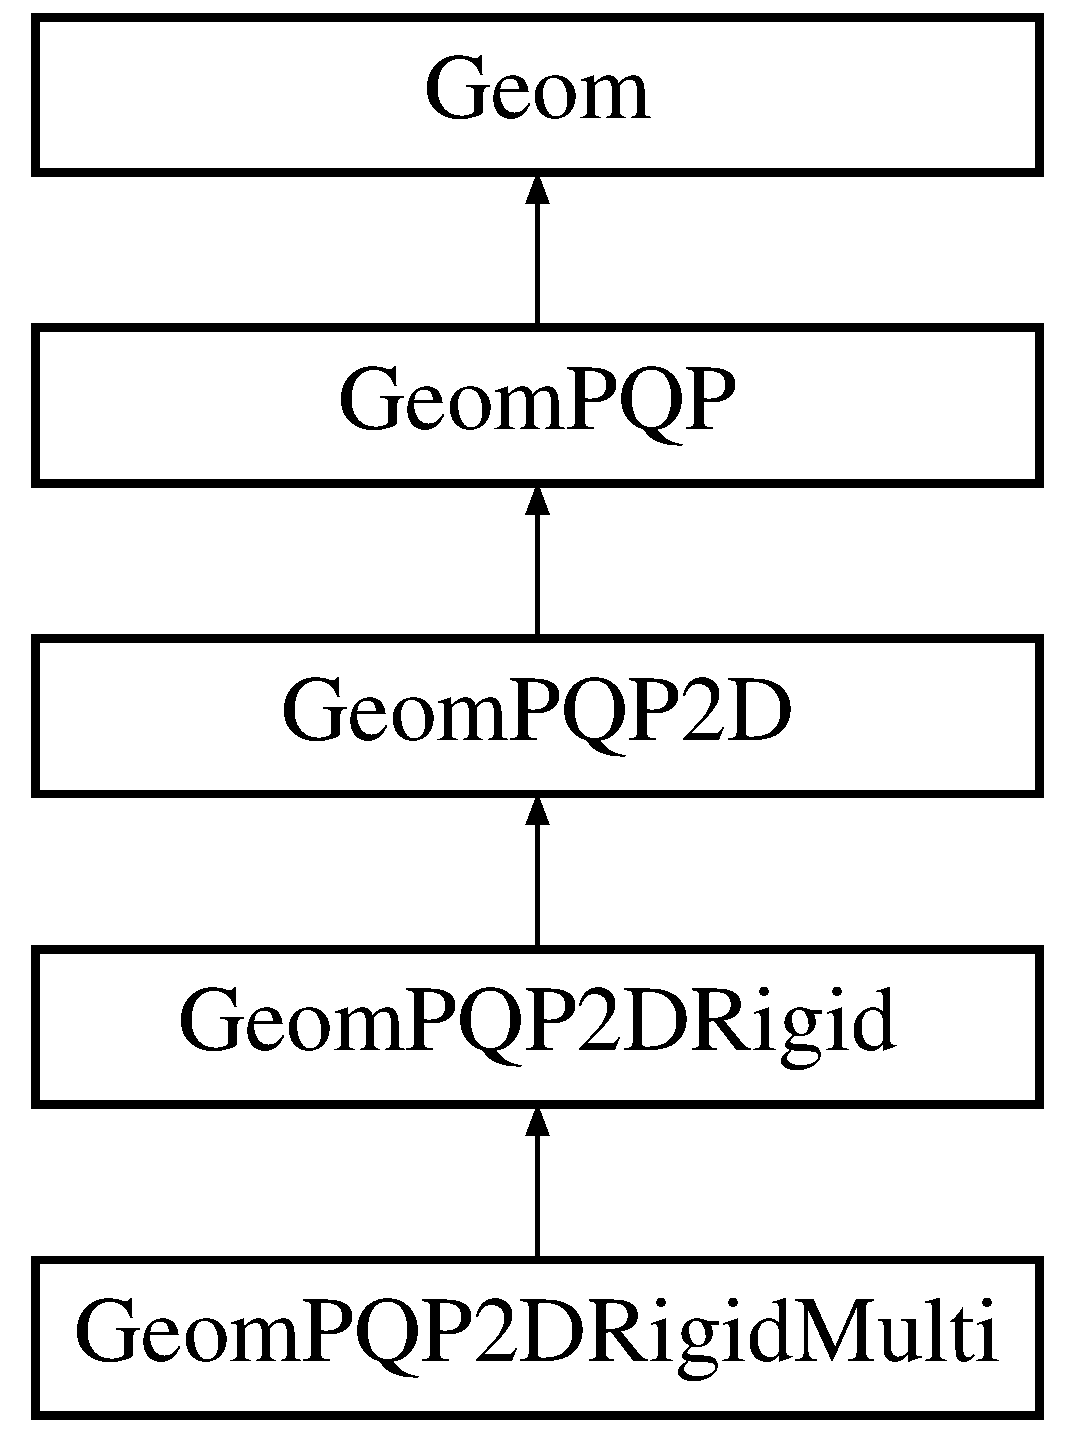
\includegraphics[height=5cm]{classGeomPQP2D}
\end{center}
\end{figure}
\subsection*{Public Methods}
\begin{CompactItemize}
\item 
{\bf Geom\-PQP2D} (string path)
\item 
virtual {\bf $\sim$Geom\-PQP2D} ()
\item 
virtual void {\bf Load\-Environment} (string path)
\item 
virtual void {\bf Load\-Robot} (string path)
\end{CompactItemize}
\subsection*{Public Attributes}
\begin{CompactItemize}
\item 
{\bf list}$<${\bf MSLPolygon}$>$ {\bf Obst\-Polygons}
\item 
{\bf list}$<${\bf MSLPolygon}$>$ {\bf Robot\-Polygons}
\end{CompactItemize}


\subsection{Detailed Description}
A parent class for 2D PQP geometries.



\subsection{Constructor \& Destructor Documentation}
\index{GeomPQP2D@{Geom\-PQP2D}!GeomPQP2D@{GeomPQP2D}}
\index{GeomPQP2D@{GeomPQP2D}!GeomPQP2D@{Geom\-PQP2D}}
\subsubsection{\setlength{\rightskip}{0pt plus 5cm}Geom\-PQP2D::Geom\-PQP2D (string {\em path} = \char`\"{}\char`\"{})}\label{classGeomPQP2D_a0}


\index{GeomPQP2D@{Geom\-PQP2D}!~GeomPQP2D@{$\sim$GeomPQP2D}}
\index{~GeomPQP2D@{$\sim$GeomPQP2D}!GeomPQP2D@{Geom\-PQP2D}}
\subsubsection{\setlength{\rightskip}{0pt plus 5cm}Geom\-PQP2D::$\sim$Geom\-PQP2D ()\hspace{0.3cm}{\tt  [inline, virtual]}}\label{classGeomPQP2D_a1}




\subsection{Member Function Documentation}
\index{GeomPQP2D@{Geom\-PQP2D}!LoadEnvironment@{LoadEnvironment}}
\index{LoadEnvironment@{LoadEnvironment}!GeomPQP2D@{Geom\-PQP2D}}
\subsubsection{\setlength{\rightskip}{0pt plus 5cm}void Geom\-PQP2D::Load\-Environment (string {\em path})\hspace{0.3cm}{\tt  [virtual]}}\label{classGeomPQP2D_a2}




Reimplemented from {\bf Geom\-PQP} {\rm (p.\,\pageref{classGeomPQP_a2})}.\index{GeomPQP2D@{Geom\-PQP2D}!LoadRobot@{LoadRobot}}
\index{LoadRobot@{LoadRobot}!GeomPQP2D@{Geom\-PQP2D}}
\subsubsection{\setlength{\rightskip}{0pt plus 5cm}void Geom\-PQP2D::Load\-Robot (string {\em path})\hspace{0.3cm}{\tt  [virtual]}}\label{classGeomPQP2D_a3}




Reimplemented from {\bf Geom\-PQP} {\rm (p.\,\pageref{classGeomPQP_a3})}.

Reimplemented in {\bf Geom\-PQP2DRigid\-Multi} {\rm (p.\,\pageref{classGeomPQP2DRigidMulti_a4})}.

\subsection{Member Data Documentation}
\index{GeomPQP2D@{Geom\-PQP2D}!ObstPolygons@{ObstPolygons}}
\index{ObstPolygons@{ObstPolygons}!GeomPQP2D@{Geom\-PQP2D}}
\subsubsection{\setlength{\rightskip}{0pt plus 5cm}{\bf list}$<$ {\bf MSLPolygon} $>$ Geom\-PQP2D::Obst\-Polygons$<${\bf MSLPolygon}$>$}\label{classGeomPQP2D_m0}


\index{GeomPQP2D@{Geom\-PQP2D}!RobotPolygons@{RobotPolygons}}
\index{RobotPolygons@{RobotPolygons}!GeomPQP2D@{Geom\-PQP2D}}
\subsubsection{\setlength{\rightskip}{0pt plus 5cm}{\bf list}$<$ {\bf MSLPolygon} $>$ Geom\-PQP2D::Robot\-Polygons$<${\bf MSLPolygon}$>$}\label{classGeomPQP2D_m1}




The documentation for this class was generated from the following files:\begin{CompactItemize}
\item 
{\bf geom\-PQP.h}\item 
{\bf geom\-PQP.C}\end{CompactItemize}

\section{Geom\-PQP2DRigid  Class Reference}
\label{classGeomPQP2DRigid}\index{GeomPQP2DRigid@{Geom\-PQP2DRigid}}
2D rigid body. 


{\tt \#include $<$geom\-PQP.h$>$}

Inheritance diagram for Geom\-PQP2DRigid::\begin{figure}[H]
\begin{center}
\leavevmode
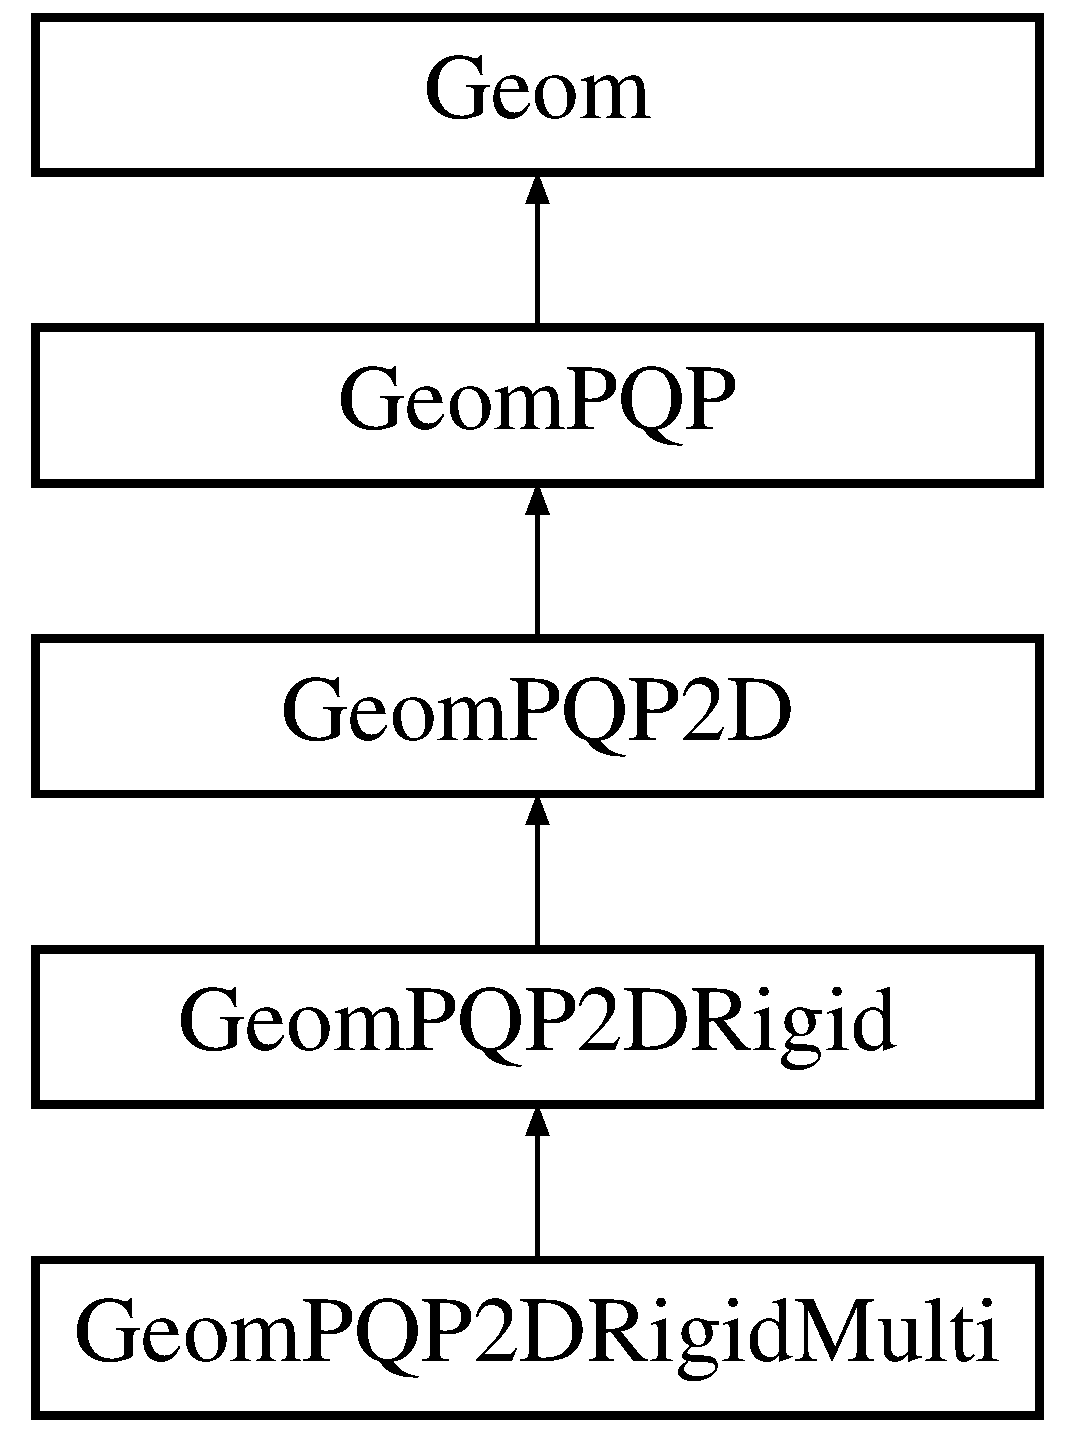
\includegraphics[height=5cm]{classGeomPQP2DRigid}
\end{center}
\end{figure}
\subsection*{Public Methods}
\begin{CompactItemize}
\item 
{\bf Geom\-PQP2DRigid} (string path)
\item 
virtual {\bf $\sim$Geom\-PQP2DRigid} ()
\item 
virtual bool {\bf Collision\-Free} (const {\bf MSLVector} \&q)
\begin{CompactList}\small\item\em Return true if the robot(s) and obstacles are not in collision.\item\end{CompactList}\item 
virtual double {\bf Distance\-Comp} (const {\bf MSLVector} \&q)
\begin{CompactList}\small\item\em Compute the distance of the closest point on the robot to the obstacle region.\item\end{CompactList}\item 
virtual {\bf MSLVector} {\bf Configuration\-Difference} (const {\bf MSLVector} \&q1, const {\bf MSLVector} \&q2)
\begin{CompactList}\small\item\em Compute a {\bf MSLVector} {\rm (p.\,\pageref{classMSLVector})} based on q2-q1. In R$^\wedge$n, the configurations are simply subtracted to make the {\bf MSLVector} {\rm (p.\,\pageref{classMSLVector})}. This method exists to make things work correctly for other configuration-space topologies.\item\end{CompactList}\item 
void {\bf Set\-Transformation} (const {\bf MSLVector} \&q)
\end{CompactItemize}


\subsection{Detailed Description}
2D rigid body.



\subsection{Constructor \& Destructor Documentation}
\index{GeomPQP2DRigid@{Geom\-PQP2DRigid}!GeomPQP2DRigid@{GeomPQP2DRigid}}
\index{GeomPQP2DRigid@{GeomPQP2DRigid}!GeomPQP2DRigid@{Geom\-PQP2DRigid}}
\subsubsection{\setlength{\rightskip}{0pt plus 5cm}Geom\-PQP2DRigid::Geom\-PQP2DRigid (string {\em path} = \char`\"{}\char`\"{})}\label{classGeomPQP2DRigid_a0}


\index{GeomPQP2DRigid@{Geom\-PQP2DRigid}!~GeomPQP2DRigid@{$\sim$GeomPQP2DRigid}}
\index{~GeomPQP2DRigid@{$\sim$GeomPQP2DRigid}!GeomPQP2DRigid@{Geom\-PQP2DRigid}}
\subsubsection{\setlength{\rightskip}{0pt plus 5cm}Geom\-PQP2DRigid::$\sim$Geom\-PQP2DRigid ()\hspace{0.3cm}{\tt  [inline, virtual]}}\label{classGeomPQP2DRigid_a1}




\subsection{Member Function Documentation}
\index{GeomPQP2DRigid@{Geom\-PQP2DRigid}!CollisionFree@{CollisionFree}}
\index{CollisionFree@{CollisionFree}!GeomPQP2DRigid@{Geom\-PQP2DRigid}}
\subsubsection{\setlength{\rightskip}{0pt plus 5cm}bool Geom\-PQP2DRigid::Collision\-Free (const {\bf MSLVector} \& {\em q})\hspace{0.3cm}{\tt  [virtual]}}\label{classGeomPQP2DRigid_a2}


Return true if the robot(s) and obstacles are not in collision.



Reimplemented from {\bf Geom\-PQP} {\rm (p.\,\pageref{classGeomPQP_a4})}.

Reimplemented in {\bf Geom\-PQP2DRigid\-Multi} {\rm (p.\,\pageref{classGeomPQP2DRigidMulti_a2})}.\index{GeomPQP2DRigid@{Geom\-PQP2DRigid}!ConfigurationDifference@{ConfigurationDifference}}
\index{ConfigurationDifference@{ConfigurationDifference}!GeomPQP2DRigid@{Geom\-PQP2DRigid}}
\subsubsection{\setlength{\rightskip}{0pt plus 5cm}{\bf MSLVector} Geom\-PQP2DRigid::Configuration\-Difference (const {\bf MSLVector} \& {\em q1}, const {\bf MSLVector} \& {\em q2})\hspace{0.3cm}{\tt  [virtual]}}\label{classGeomPQP2DRigid_a4}


Compute a {\bf MSLVector} {\rm (p.\,\pageref{classMSLVector})} based on q2-q1. In R$^\wedge$n, the configurations are simply subtracted to make the {\bf MSLVector} {\rm (p.\,\pageref{classMSLVector})}. This method exists to make things work correctly for other configuration-space topologies.



Reimplemented from {\bf Geom} {\rm (p.\,\pageref{classGeom_a4})}.\index{GeomPQP2DRigid@{Geom\-PQP2DRigid}!DistanceComp@{DistanceComp}}
\index{DistanceComp@{DistanceComp}!GeomPQP2DRigid@{Geom\-PQP2DRigid}}
\subsubsection{\setlength{\rightskip}{0pt plus 5cm}double Geom\-PQP2DRigid::Distance\-Comp (const {\bf MSLVector} \& {\em q})\hspace{0.3cm}{\tt  [virtual]}}\label{classGeomPQP2DRigid_a3}


Compute the distance of the closest point on the robot to the obstacle region.



Reimplemented from {\bf Geom\-PQP} {\rm (p.\,\pageref{classGeomPQP_a5})}.

Reimplemented in {\bf Geom\-PQP2DRigid\-Multi} {\rm (p.\,\pageref{classGeomPQP2DRigidMulti_a3})}.\index{GeomPQP2DRigid@{Geom\-PQP2DRigid}!SetTransformation@{SetTransformation}}
\index{SetTransformation@{SetTransformation}!GeomPQP2DRigid@{Geom\-PQP2DRigid}}
\subsubsection{\setlength{\rightskip}{0pt plus 5cm}void Geom\-PQP2DRigid::Set\-Transformation (const {\bf MSLVector} \& {\em q})}\label{classGeomPQP2DRigid_a5}




Reimplemented in {\bf Geom\-PQP2DRigid\-Multi} {\rm (p.\,\pageref{classGeomPQP2DRigidMulti_a5})}.

The documentation for this class was generated from the following files:\begin{CompactItemize}
\item 
{\bf geom\-PQP.h}\item 
{\bf geom\-PQP.C}\end{CompactItemize}

\section{Geom\-PQP2DRigid\-Multi  Class Reference}
\label{classGeomPQP2DRigidMulti}\index{GeomPQP2DRigidMulti@{Geom\-PQP2DRigid\-Multi}}
A collection of 2D rigid bodies. 


{\tt \#include $<$geom\-PQP.h$>$}

Inheritance diagram for Geom\-PQP2DRigid\-Multi::\begin{figure}[H]
\begin{center}
\leavevmode
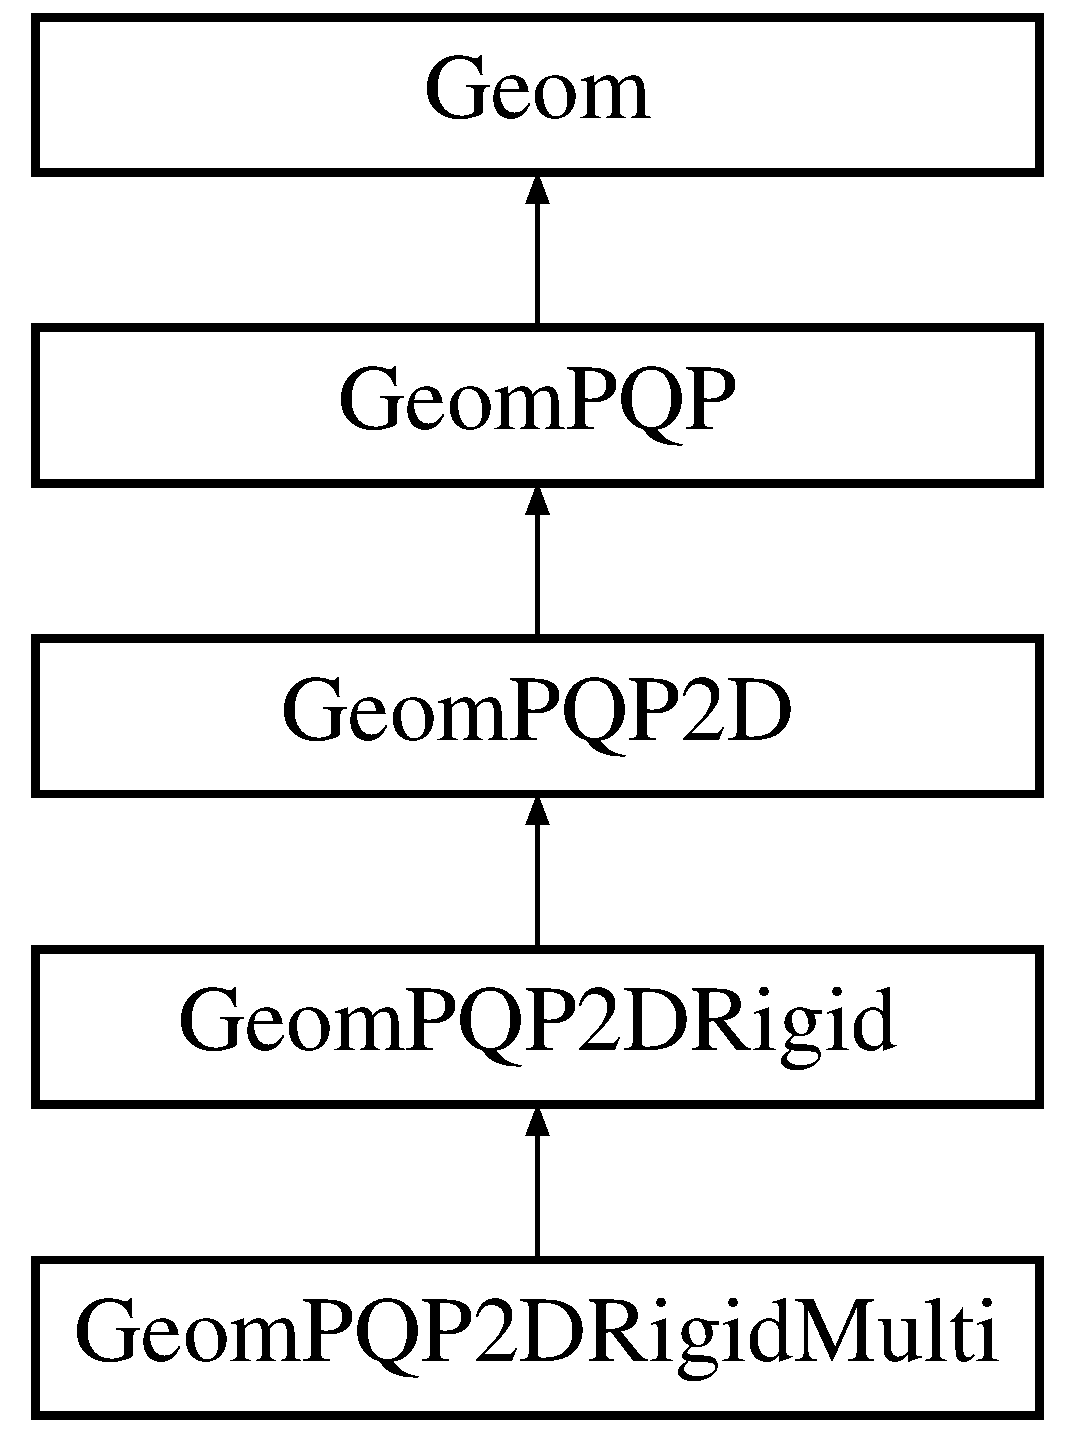
\includegraphics[height=5cm]{classGeomPQP2DRigidMulti}
\end{center}
\end{figure}
\subsection*{Public Methods}
\begin{CompactItemize}
\item 
{\bf Geom\-PQP2DRigid\-Multi} (string path)
\item 
virtual {\bf $\sim$Geom\-PQP2DRigid\-Multi} ()
\item 
virtual bool {\bf Collision\-Free} (const {\bf MSLVector} \&q)
\begin{CompactList}\small\item\em Return true if the robot(s) and obstacles are not in collision.\item\end{CompactList}\item 
virtual double {\bf Distance\-Comp} (const {\bf MSLVector} \&q)
\begin{CompactList}\small\item\em Compute the distance of the closest point on the robot to the obstacle region.\item\end{CompactList}\item 
virtual void {\bf Load\-Robot} (string path)
\item 
void {\bf Set\-Transformation} (const {\bf MSLVector} \&q)
\end{CompactItemize}
\subsection*{Public Attributes}
\begin{CompactItemize}
\item 
bool {\bf Self\-Collision\-Check}
\end{CompactItemize}


\subsection{Detailed Description}
A collection of 2D rigid bodies.



\subsection{Constructor \& Destructor Documentation}
\index{GeomPQP2DRigidMulti@{Geom\-PQP2DRigid\-Multi}!GeomPQP2DRigidMulti@{GeomPQP2DRigidMulti}}
\index{GeomPQP2DRigidMulti@{GeomPQP2DRigidMulti}!GeomPQP2DRigidMulti@{Geom\-PQP2DRigid\-Multi}}
\subsubsection{\setlength{\rightskip}{0pt plus 5cm}Geom\-PQP2DRigid\-Multi::Geom\-PQP2DRigid\-Multi (string {\em path} = \char`\"{}\char`\"{})}\label{classGeomPQP2DRigidMulti_a0}


\index{GeomPQP2DRigidMulti@{Geom\-PQP2DRigid\-Multi}!~GeomPQP2DRigidMulti@{$\sim$GeomPQP2DRigidMulti}}
\index{~GeomPQP2DRigidMulti@{$\sim$GeomPQP2DRigidMulti}!GeomPQP2DRigidMulti@{Geom\-PQP2DRigid\-Multi}}
\subsubsection{\setlength{\rightskip}{0pt plus 5cm}Geom\-PQP2DRigid\-Multi::$\sim$Geom\-PQP2DRigid\-Multi ()\hspace{0.3cm}{\tt  [inline, virtual]}}\label{classGeomPQP2DRigidMulti_a1}




\subsection{Member Function Documentation}
\index{GeomPQP2DRigidMulti@{Geom\-PQP2DRigid\-Multi}!CollisionFree@{CollisionFree}}
\index{CollisionFree@{CollisionFree}!GeomPQP2DRigidMulti@{Geom\-PQP2DRigid\-Multi}}
\subsubsection{\setlength{\rightskip}{0pt plus 5cm}bool Geom\-PQP2DRigid\-Multi::Collision\-Free (const {\bf MSLVector} \& {\em q})\hspace{0.3cm}{\tt  [virtual]}}\label{classGeomPQP2DRigidMulti_a2}


Return true if the robot(s) and obstacles are not in collision.



Reimplemented from {\bf Geom\-PQP2DRigid} {\rm (p.\,\pageref{classGeomPQP2DRigid_a2})}.\index{GeomPQP2DRigidMulti@{Geom\-PQP2DRigid\-Multi}!DistanceComp@{DistanceComp}}
\index{DistanceComp@{DistanceComp}!GeomPQP2DRigidMulti@{Geom\-PQP2DRigid\-Multi}}
\subsubsection{\setlength{\rightskip}{0pt plus 5cm}double Geom\-PQP2DRigid\-Multi::Distance\-Comp (const {\bf MSLVector} \& {\em q})\hspace{0.3cm}{\tt  [virtual]}}\label{classGeomPQP2DRigidMulti_a3}


Compute the distance of the closest point on the robot to the obstacle region.



Reimplemented from {\bf Geom\-PQP2DRigid} {\rm (p.\,\pageref{classGeomPQP2DRigid_a3})}.\index{GeomPQP2DRigidMulti@{Geom\-PQP2DRigid\-Multi}!LoadRobot@{LoadRobot}}
\index{LoadRobot@{LoadRobot}!GeomPQP2DRigidMulti@{Geom\-PQP2DRigid\-Multi}}
\subsubsection{\setlength{\rightskip}{0pt plus 5cm}void Geom\-PQP2DRigid\-Multi::Load\-Robot (string {\em path})\hspace{0.3cm}{\tt  [virtual]}}\label{classGeomPQP2DRigidMulti_a4}




Reimplemented from {\bf Geom\-PQP2D} {\rm (p.\,\pageref{classGeomPQP2D_a3})}.\index{GeomPQP2DRigidMulti@{Geom\-PQP2DRigid\-Multi}!SetTransformation@{SetTransformation}}
\index{SetTransformation@{SetTransformation}!GeomPQP2DRigidMulti@{Geom\-PQP2DRigid\-Multi}}
\subsubsection{\setlength{\rightskip}{0pt plus 5cm}void Geom\-PQP2DRigid\-Multi::Set\-Transformation (const {\bf MSLVector} \& {\em q})}\label{classGeomPQP2DRigidMulti_a5}




Reimplemented from {\bf Geom\-PQP2DRigid} {\rm (p.\,\pageref{classGeomPQP2DRigid_a5})}.

\subsection{Member Data Documentation}
\index{GeomPQP2DRigidMulti@{Geom\-PQP2DRigid\-Multi}!SelfCollisionCheck@{SelfCollisionCheck}}
\index{SelfCollisionCheck@{SelfCollisionCheck}!GeomPQP2DRigidMulti@{Geom\-PQP2DRigid\-Multi}}
\subsubsection{\setlength{\rightskip}{0pt plus 5cm}bool Geom\-PQP2DRigid\-Multi::Self\-Collision\-Check}\label{classGeomPQP2DRigidMulti_m0}




The documentation for this class was generated from the following files:\begin{CompactItemize}
\item 
{\bf geom\-PQP.h}\item 
{\bf geom\-PQP.C}\end{CompactItemize}

\section{Geom\-PQP3DRigid  Class Reference}
\label{classGeomPQP3DRigid}\index{GeomPQP3DRigid@{Geom\-PQP3DRigid}}
3D rigid body. 


{\tt \#include $<$geom\-PQP.h$>$}

Inheritance diagram for Geom\-PQP3DRigid::\begin{figure}[H]
\begin{center}
\leavevmode
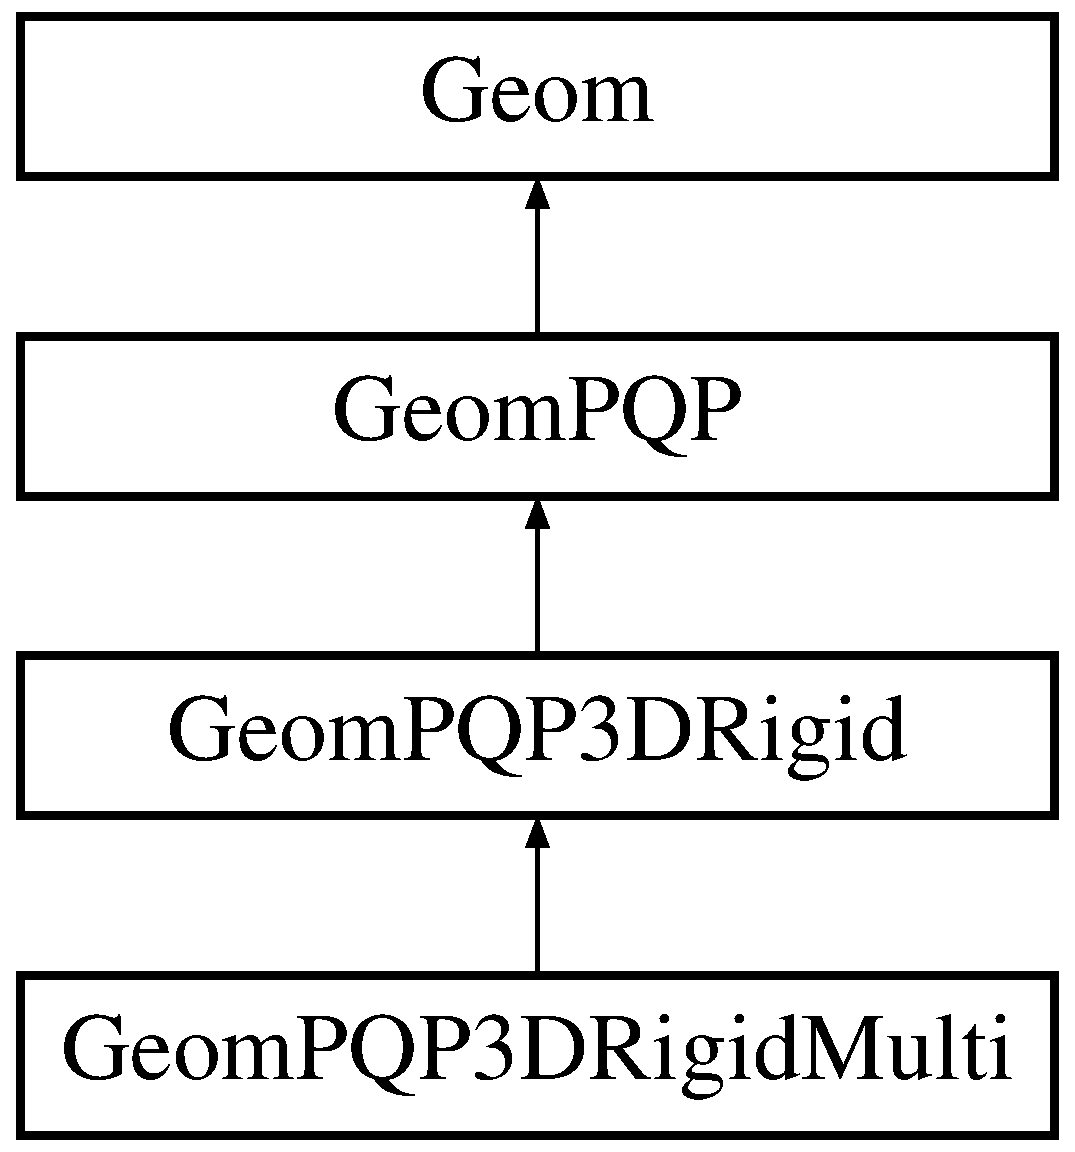
\includegraphics[height=4cm]{classGeomPQP3DRigid}
\end{center}
\end{figure}
\subsection*{Public Methods}
\begin{CompactItemize}
\item 
{\bf Geom\-PQP3DRigid} (string path)
\item 
virtual {\bf $\sim$Geom\-PQP3DRigid} ()
\item 
virtual bool {\bf Collision\-Free} (const {\bf MSLVector} \&q)
\begin{CompactList}\small\item\em Return true if the robot(s) and obstacles are not in collision.\item\end{CompactList}\item 
virtual double {\bf Distance\-Comp} (const {\bf MSLVector} \&q)
\begin{CompactList}\small\item\em Compute the distance of the closest point on the robot to the obstacle region.\item\end{CompactList}\item 
virtual {\bf MSLVector} {\bf Configuration\-Difference} (const {\bf MSLVector} \&q1, const {\bf MSLVector} \&q2)
\begin{CompactList}\small\item\em Compute a {\bf MSLVector} {\rm (p.\,\pageref{classMSLVector})} based on q2-q1. In R$^\wedge$n, the configurations are simply subtracted to make the {\bf MSLVector} {\rm (p.\,\pageref{classMSLVector})}. This method exists to make things work correctly for other configuration-space topologies.\item\end{CompactList}\item 
void {\bf Set\-Transformation} (const {\bf MSLVector} \&q)
\end{CompactItemize}


\subsection{Detailed Description}
3D rigid body.



\subsection{Constructor \& Destructor Documentation}
\index{GeomPQP3DRigid@{Geom\-PQP3DRigid}!GeomPQP3DRigid@{GeomPQP3DRigid}}
\index{GeomPQP3DRigid@{GeomPQP3DRigid}!GeomPQP3DRigid@{Geom\-PQP3DRigid}}
\subsubsection{\setlength{\rightskip}{0pt plus 5cm}Geom\-PQP3DRigid::Geom\-PQP3DRigid (string {\em path} = \char`\"{}\char`\"{})}\label{classGeomPQP3DRigid_a0}


\index{GeomPQP3DRigid@{Geom\-PQP3DRigid}!~GeomPQP3DRigid@{$\sim$GeomPQP3DRigid}}
\index{~GeomPQP3DRigid@{$\sim$GeomPQP3DRigid}!GeomPQP3DRigid@{Geom\-PQP3DRigid}}
\subsubsection{\setlength{\rightskip}{0pt plus 5cm}Geom\-PQP3DRigid::$\sim$Geom\-PQP3DRigid ()\hspace{0.3cm}{\tt  [inline, virtual]}}\label{classGeomPQP3DRigid_a1}




\subsection{Member Function Documentation}
\index{GeomPQP3DRigid@{Geom\-PQP3DRigid}!CollisionFree@{CollisionFree}}
\index{CollisionFree@{CollisionFree}!GeomPQP3DRigid@{Geom\-PQP3DRigid}}
\subsubsection{\setlength{\rightskip}{0pt plus 5cm}bool Geom\-PQP3DRigid::Collision\-Free (const {\bf MSLVector} \& {\em q})\hspace{0.3cm}{\tt  [virtual]}}\label{classGeomPQP3DRigid_a2}


Return true if the robot(s) and obstacles are not in collision.



Reimplemented from {\bf Geom\-PQP} {\rm (p.\,\pageref{classGeomPQP_a4})}.

Reimplemented in {\bf Geom\-PQP3DRigid\-Multi} {\rm (p.\,\pageref{classGeomPQP3DRigidMulti_a2})}.\index{GeomPQP3DRigid@{Geom\-PQP3DRigid}!ConfigurationDifference@{ConfigurationDifference}}
\index{ConfigurationDifference@{ConfigurationDifference}!GeomPQP3DRigid@{Geom\-PQP3DRigid}}
\subsubsection{\setlength{\rightskip}{0pt plus 5cm}{\bf MSLVector} Geom\-PQP3DRigid::Configuration\-Difference (const {\bf MSLVector} \& {\em q1}, const {\bf MSLVector} \& {\em q2})\hspace{0.3cm}{\tt  [virtual]}}\label{classGeomPQP3DRigid_a4}


Compute a {\bf MSLVector} {\rm (p.\,\pageref{classMSLVector})} based on q2-q1. In R$^\wedge$n, the configurations are simply subtracted to make the {\bf MSLVector} {\rm (p.\,\pageref{classMSLVector})}. This method exists to make things work correctly for other configuration-space topologies.



Reimplemented from {\bf Geom} {\rm (p.\,\pageref{classGeom_a4})}.\index{GeomPQP3DRigid@{Geom\-PQP3DRigid}!DistanceComp@{DistanceComp}}
\index{DistanceComp@{DistanceComp}!GeomPQP3DRigid@{Geom\-PQP3DRigid}}
\subsubsection{\setlength{\rightskip}{0pt plus 5cm}double Geom\-PQP3DRigid::Distance\-Comp (const {\bf MSLVector} \& {\em q})\hspace{0.3cm}{\tt  [virtual]}}\label{classGeomPQP3DRigid_a3}


Compute the distance of the closest point on the robot to the obstacle region.



Reimplemented from {\bf Geom\-PQP} {\rm (p.\,\pageref{classGeomPQP_a5})}.

Reimplemented in {\bf Geom\-PQP3DRigid\-Multi} {\rm (p.\,\pageref{classGeomPQP3DRigidMulti_a3})}.\index{GeomPQP3DRigid@{Geom\-PQP3DRigid}!SetTransformation@{SetTransformation}}
\index{SetTransformation@{SetTransformation}!GeomPQP3DRigid@{Geom\-PQP3DRigid}}
\subsubsection{\setlength{\rightskip}{0pt plus 5cm}void Geom\-PQP3DRigid::Set\-Transformation (const {\bf MSLVector} \& {\em q})}\label{classGeomPQP3DRigid_a5}




Reimplemented in {\bf Geom\-PQP3DRigid\-Multi} {\rm (p.\,\pageref{classGeomPQP3DRigidMulti_a5})}.

The documentation for this class was generated from the following files:\begin{CompactItemize}
\item 
{\bf geom\-PQP.h}\item 
{\bf geom\-PQP.C}\end{CompactItemize}

\section{Geom\-PQP3DRigid\-Multi  Class Reference}
\label{classGeomPQP3DRigidMulti}\index{GeomPQP3DRigidMulti@{Geom\-PQP3DRigid\-Multi}}
A collection of 3D rigid modies. 


{\tt \#include $<$geom\-PQP.h$>$}

Inheritance diagram for Geom\-PQP3DRigid\-Multi::\begin{figure}[H]
\begin{center}
\leavevmode
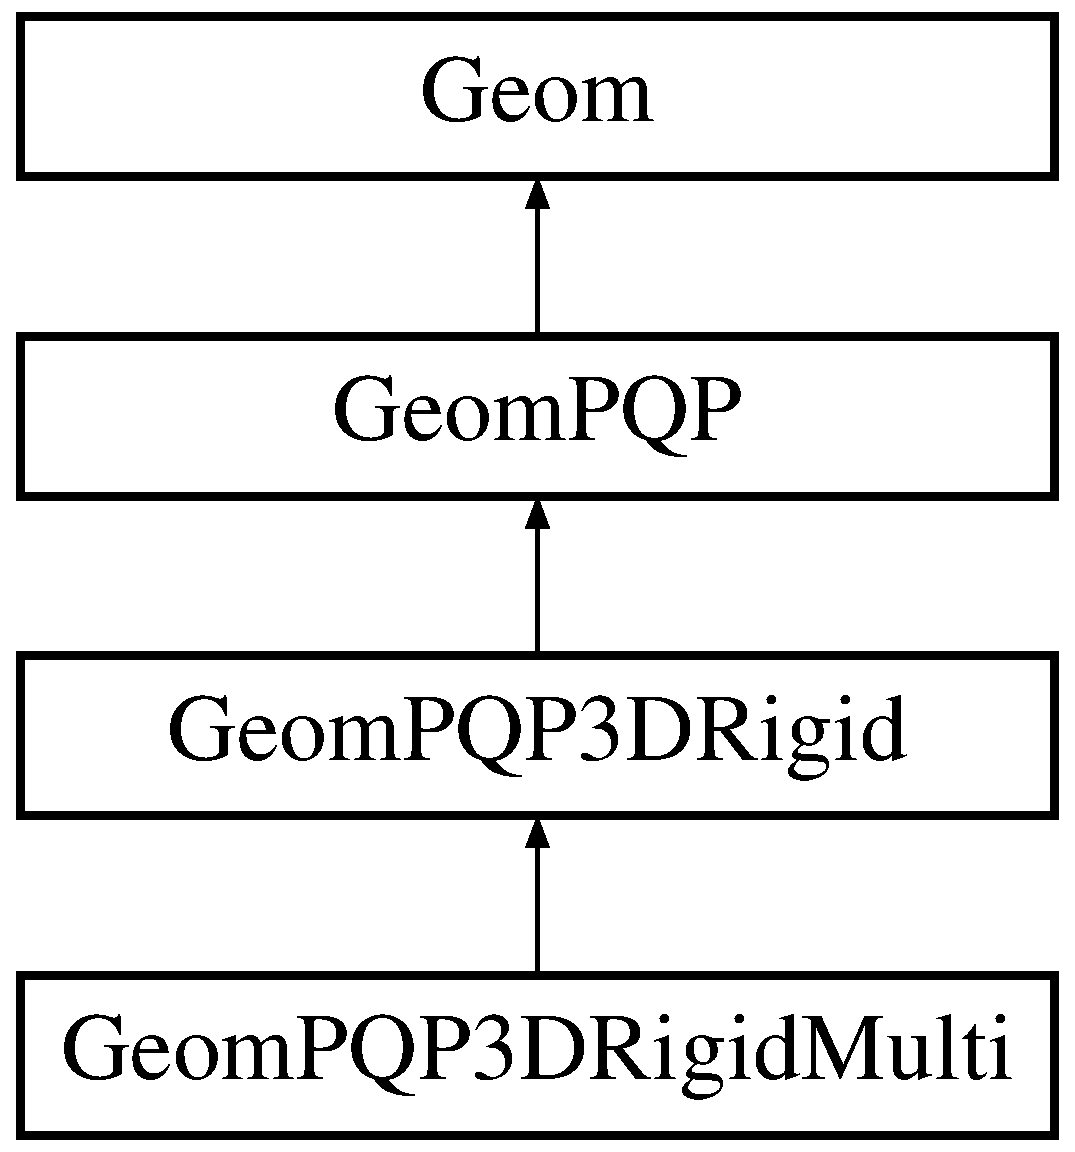
\includegraphics[height=4cm]{classGeomPQP3DRigidMulti}
\end{center}
\end{figure}
\subsection*{Public Methods}
\begin{CompactItemize}
\item 
{\bf Geom\-PQP3DRigid\-Multi} (string path)
\item 
virtual {\bf $\sim$Geom\-PQP3DRigid\-Multi} ()
\item 
virtual bool {\bf Collision\-Free} (const {\bf MSLVector} \&q)
\begin{CompactList}\small\item\em Return true if the robot(s) and obstacles are not in collision.\item\end{CompactList}\item 
virtual double {\bf Distance\-Comp} (const {\bf MSLVector} \&q)
\begin{CompactList}\small\item\em Compute the distance of the closest point on the robot to the obstacle region.\item\end{CompactList}\item 
virtual void {\bf Load\-Robot} (string path)
\item 
void {\bf Set\-Transformation} (const {\bf MSLVector} \&q)
\end{CompactItemize}
\subsection*{Public Attributes}
\begin{CompactItemize}
\item 
bool {\bf Self\-Collision\-Check}
\end{CompactItemize}


\subsection{Detailed Description}
A collection of 3D rigid modies.



\subsection{Constructor \& Destructor Documentation}
\index{GeomPQP3DRigidMulti@{Geom\-PQP3DRigid\-Multi}!GeomPQP3DRigidMulti@{GeomPQP3DRigidMulti}}
\index{GeomPQP3DRigidMulti@{GeomPQP3DRigidMulti}!GeomPQP3DRigidMulti@{Geom\-PQP3DRigid\-Multi}}
\subsubsection{\setlength{\rightskip}{0pt plus 5cm}Geom\-PQP3DRigid\-Multi::Geom\-PQP3DRigid\-Multi (string {\em path} = \char`\"{}\char`\"{})}\label{classGeomPQP3DRigidMulti_a0}


\index{GeomPQP3DRigidMulti@{Geom\-PQP3DRigid\-Multi}!~GeomPQP3DRigidMulti@{$\sim$GeomPQP3DRigidMulti}}
\index{~GeomPQP3DRigidMulti@{$\sim$GeomPQP3DRigidMulti}!GeomPQP3DRigidMulti@{Geom\-PQP3DRigid\-Multi}}
\subsubsection{\setlength{\rightskip}{0pt plus 5cm}Geom\-PQP3DRigid\-Multi::$\sim$Geom\-PQP3DRigid\-Multi ()\hspace{0.3cm}{\tt  [inline, virtual]}}\label{classGeomPQP3DRigidMulti_a1}




\subsection{Member Function Documentation}
\index{GeomPQP3DRigidMulti@{Geom\-PQP3DRigid\-Multi}!CollisionFree@{CollisionFree}}
\index{CollisionFree@{CollisionFree}!GeomPQP3DRigidMulti@{Geom\-PQP3DRigid\-Multi}}
\subsubsection{\setlength{\rightskip}{0pt plus 5cm}bool Geom\-PQP3DRigid\-Multi::Collision\-Free (const {\bf MSLVector} \& {\em q})\hspace{0.3cm}{\tt  [virtual]}}\label{classGeomPQP3DRigidMulti_a2}


Return true if the robot(s) and obstacles are not in collision.



Reimplemented from {\bf Geom\-PQP3DRigid} {\rm (p.\,\pageref{classGeomPQP3DRigid_a2})}.\index{GeomPQP3DRigidMulti@{Geom\-PQP3DRigid\-Multi}!DistanceComp@{DistanceComp}}
\index{DistanceComp@{DistanceComp}!GeomPQP3DRigidMulti@{Geom\-PQP3DRigid\-Multi}}
\subsubsection{\setlength{\rightskip}{0pt plus 5cm}double Geom\-PQP3DRigid\-Multi::Distance\-Comp (const {\bf MSLVector} \& {\em q})\hspace{0.3cm}{\tt  [virtual]}}\label{classGeomPQP3DRigidMulti_a3}


Compute the distance of the closest point on the robot to the obstacle region.



Reimplemented from {\bf Geom\-PQP3DRigid} {\rm (p.\,\pageref{classGeomPQP3DRigid_a3})}.\index{GeomPQP3DRigidMulti@{Geom\-PQP3DRigid\-Multi}!LoadRobot@{LoadRobot}}
\index{LoadRobot@{LoadRobot}!GeomPQP3DRigidMulti@{Geom\-PQP3DRigid\-Multi}}
\subsubsection{\setlength{\rightskip}{0pt plus 5cm}void Geom\-PQP3DRigid\-Multi::Load\-Robot (string {\em path})\hspace{0.3cm}{\tt  [virtual]}}\label{classGeomPQP3DRigidMulti_a4}




Reimplemented from {\bf Geom\-PQP} {\rm (p.\,\pageref{classGeomPQP_a3})}.\index{GeomPQP3DRigidMulti@{Geom\-PQP3DRigid\-Multi}!SetTransformation@{SetTransformation}}
\index{SetTransformation@{SetTransformation}!GeomPQP3DRigidMulti@{Geom\-PQP3DRigid\-Multi}}
\subsubsection{\setlength{\rightskip}{0pt plus 5cm}void Geom\-PQP3DRigid\-Multi::Set\-Transformation (const {\bf MSLVector} \& {\em q})}\label{classGeomPQP3DRigidMulti_a5}




Reimplemented from {\bf Geom\-PQP3DRigid} {\rm (p.\,\pageref{classGeomPQP3DRigid_a5})}.

\subsection{Member Data Documentation}
\index{GeomPQP3DRigidMulti@{Geom\-PQP3DRigid\-Multi}!SelfCollisionCheck@{SelfCollisionCheck}}
\index{SelfCollisionCheck@{SelfCollisionCheck}!GeomPQP3DRigidMulti@{Geom\-PQP3DRigid\-Multi}}
\subsubsection{\setlength{\rightskip}{0pt plus 5cm}bool Geom\-PQP3DRigid\-Multi::Self\-Collision\-Check}\label{classGeomPQP3DRigidMulti_m0}




The documentation for this class was generated from the following files:\begin{CompactItemize}
\item 
{\bf geom\-PQP.h}\item 
{\bf geom\-PQP.C}\end{CompactItemize}

\section{Gui  Class Reference}
\label{classGui}\index{Gui@{Gui}}
A generic class for designing graphical user interfaces (GUIs). 


{\tt \#include $<$gui.h$>$}

Inheritance diagram for Gui::\begin{figure}[H]
\begin{center}
\leavevmode
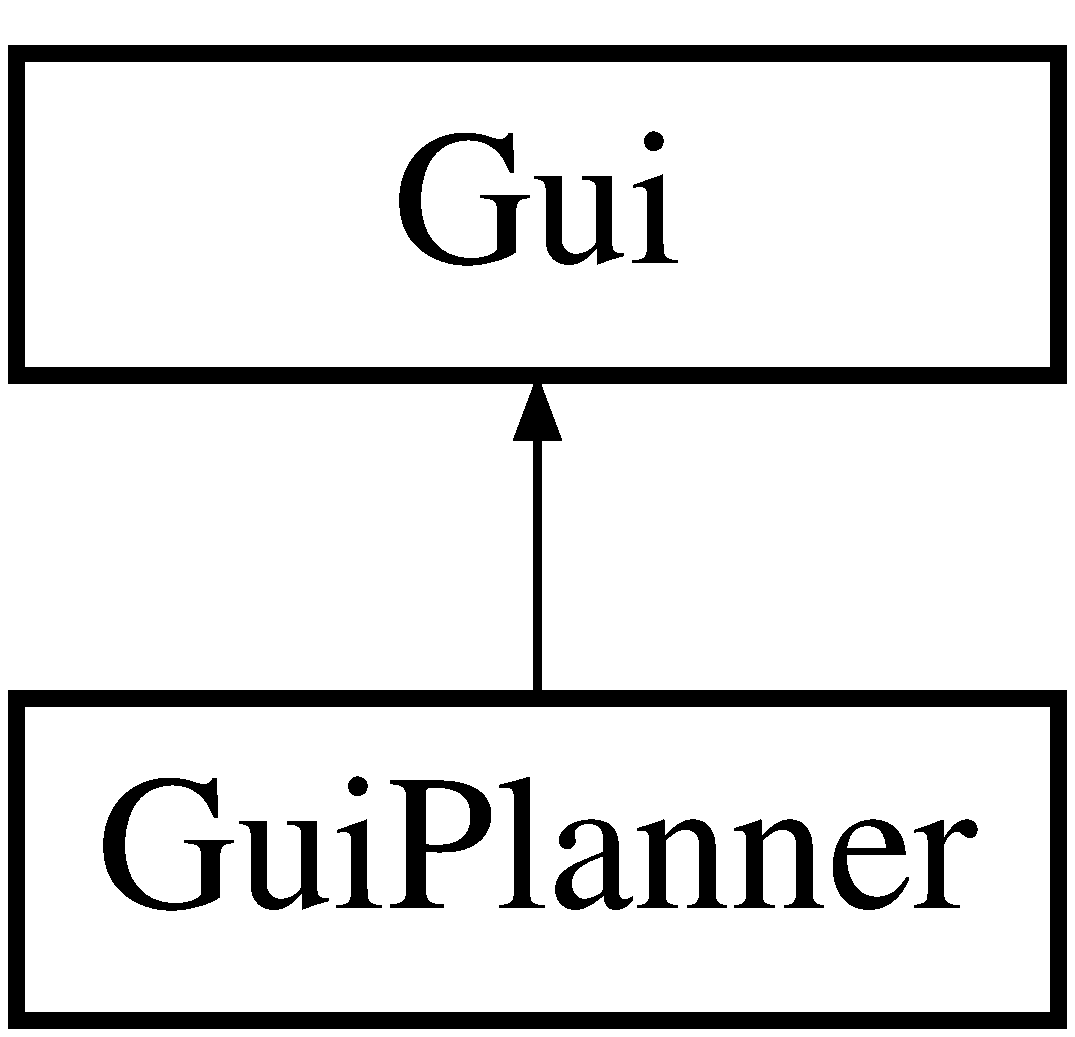
\includegraphics[height=2cm]{classGui}
\end{center}
\end{figure}
\subsection*{Public Methods}
\begin{CompactItemize}
\item 
{\bf Gui} ({\bf Render} $\ast$render)
\begin{CompactList}\small\item\em The window.\item\end{CompactList}\item 
virtual {\bf $\sim$Gui} ()
\item 
virtual void {\bf Start} ()
\begin{CompactList}\small\item\em Start running the Gui.\item\end{CompactList}\item 
virtual void {\bf Handle\-Events} ()=0
\begin{CompactList}\small\item\em Process any IO events (may be used by {\bf Render} {\rm (p.\,\pageref{classRender})}).\item\end{CompactList}\item 
virtual void {\bf Button\-Handle} (int b)
\begin{CompactList}\small\item\em Figure out what actions to take based on menu choices.\item\end{CompactList}\end{CompactItemize}
\subsection*{Public Attributes}
\begin{CompactItemize}
\item 
{\bf Render}$\ast$ {\bf R}
\item 
bool {\bf Finished}
\begin{CompactList}\small\item\em Set to true if you want to main loop to terminate.\item\end{CompactList}\end{CompactItemize}
\subsection*{Protected Methods}
\begin{CompactItemize}
\item 
virtual void {\bf Create\-Window} ()
\begin{CompactList}\small\item\em Make the menu window.\item\end{CompactList}\item 
virtual void {\bf Init} ()
\begin{CompactList}\small\item\em Initialize Gui and {\bf Render} {\rm (p.\,\pageref{classRender})}.\item\end{CompactList}\item 
virtual void {\bf Main\-Loop} ()
\begin{CompactList}\small\item\em The main event processing loop.\item\end{CompactList}\end{CompactItemize}
\subsection*{Protected Attributes}
\begin{CompactItemize}
\item 
string {\bf File\-Path}
\end{CompactItemize}


\subsection{Detailed Description}
A generic class for designing graphical user interfaces (GUIs).

The graphical user interface (GUI) is designed as a hierarchy of classes to enable specific user interfaces to be designed for a variety of different motion strategy problems and planning algorithms. Currently, there is one derived class which serves as the GUI for all of the {\bf RRT} {\rm (p.\,\pageref{classRRT})}-based planners. Each instance of Gui includes an instance of an {\bf RRT} {\rm (p.\,\pageref{classRRT})} {\bf Planner} {\rm (p.\,\pageref{classPlanner})} class and an instance of a {\bf Render} {\rm (p.\,\pageref{classRender})} class. Using this design, the same basic GUI design can be used, regardless of the particular rendering methods. 



\subsection{Constructor \& Destructor Documentation}
\index{Gui@{Gui}!Gui@{Gui}}
\index{Gui@{Gui}!Gui@{Gui}}
\subsubsection{\setlength{\rightskip}{0pt plus 5cm}Gui::Gui ({\bf Render} $\ast$ {\em render})}\label{classGui_a0}


The window.

\index{Gui@{Gui}!~Gui@{$\sim$Gui}}
\index{~Gui@{$\sim$Gui}!Gui@{Gui}}
\subsubsection{\setlength{\rightskip}{0pt plus 5cm}Gui::$\sim$Gui ()\hspace{0.3cm}{\tt  [inline, virtual]}}\label{classGui_a1}




\subsection{Member Function Documentation}
\index{Gui@{Gui}!ButtonHandle@{ButtonHandle}}
\index{ButtonHandle@{ButtonHandle}!Gui@{Gui}}
\subsubsection{\setlength{\rightskip}{0pt plus 5cm}void Gui::Button\-Handle (int {\em b})\hspace{0.3cm}{\tt  [inline, virtual]}}\label{classGui_a4}


Figure out what actions to take based on menu choices.



Reimplemented in {\bf Gui\-Planner} {\rm (p.\,\pageref{classGuiPlanner_a1})}.\index{Gui@{Gui}!CreateWindow@{CreateWindow}}
\index{CreateWindow@{CreateWindow}!Gui@{Gui}}
\subsubsection{\setlength{\rightskip}{0pt plus 5cm}void Gui::Create\-Window ()\hspace{0.3cm}{\tt  [inline, protected, virtual]}}\label{classGui_b0}


Make the menu window.

\index{Gui@{Gui}!HandleEvents@{HandleEvents}}
\index{HandleEvents@{HandleEvents}!Gui@{Gui}}
\subsubsection{\setlength{\rightskip}{0pt plus 5cm}void Gui::Handle\-Events ()\hspace{0.3cm}{\tt  [pure virtual]}}\label{classGui_a3}


Process any IO events (may be used by {\bf Render} {\rm (p.\,\pageref{classRender})}).



Reimplemented in {\bf Gui\-Planner} {\rm (p.\,\pageref{classGuiPlanner_a0})}.\index{Gui@{Gui}!Init@{Init}}
\index{Init@{Init}!Gui@{Gui}}
\subsubsection{\setlength{\rightskip}{0pt plus 5cm}void Gui::Init ()\hspace{0.3cm}{\tt  [protected, virtual]}}\label{classGui_b1}


Initialize Gui and {\bf Render} {\rm (p.\,\pageref{classRender})}.



Reimplemented in {\bf Gui\-Planner} {\rm (p.\,\pageref{classGuiPlanner_b0})}.\index{Gui@{Gui}!MainLoop@{MainLoop}}
\index{MainLoop@{MainLoop}!Gui@{Gui}}
\subsubsection{\setlength{\rightskip}{0pt plus 5cm}void Gui::Main\-Loop ()\hspace{0.3cm}{\tt  [protected, virtual]}}\label{classGui_b2}


The main event processing loop.

\index{Gui@{Gui}!Start@{Start}}
\index{Start@{Start}!Gui@{Gui}}
\subsubsection{\setlength{\rightskip}{0pt plus 5cm}void Gui::Start ()\hspace{0.3cm}{\tt  [virtual]}}\label{classGui_a2}


Start running the Gui.



\subsection{Member Data Documentation}
\index{Gui@{Gui}!FilePath@{FilePath}}
\index{FilePath@{FilePath}!Gui@{Gui}}
\subsubsection{\setlength{\rightskip}{0pt plus 5cm}string Gui::File\-Path\hspace{0.3cm}{\tt  [protected]}}\label{classGui_n0}


\index{Gui@{Gui}!Finished@{Finished}}
\index{Finished@{Finished}!Gui@{Gui}}
\subsubsection{\setlength{\rightskip}{0pt plus 5cm}bool Gui::Finished}\label{classGui_m1}


Set to true if you want to main loop to terminate.

\index{Gui@{Gui}!R@{R}}
\index{R@{R}!Gui@{Gui}}
\subsubsection{\setlength{\rightskip}{0pt plus 5cm}{\bf Render} $\ast$ Gui::R}\label{classGui_m0}




The documentation for this class was generated from the following files:\begin{CompactItemize}
\item 
{\bf gui.h}\item 
{\bf gui.C}\end{CompactItemize}

\section{Gui\-Planner  Class Reference}
\label{classGuiPlanner}\index{GuiPlanner@{Gui\-Planner}}
{\tt \#include $<$guiplanner.h$>$}

Inheritance diagram for Gui\-Planner::\begin{figure}[H]
\begin{center}
\leavevmode
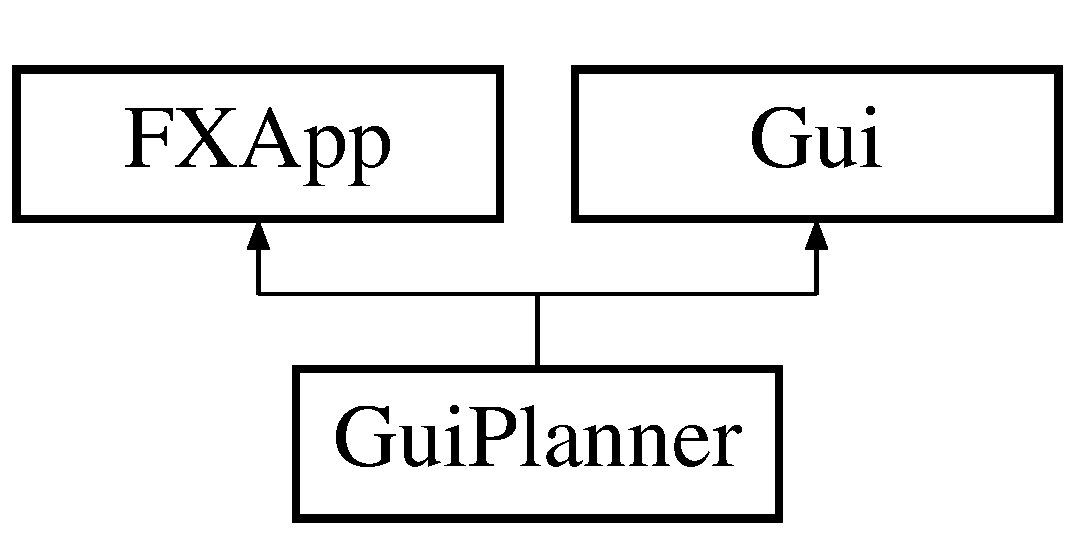
\includegraphics[height=2cm]{classGuiPlanner}
\end{center}
\end{figure}
\subsection*{Public Methods}
\begin{CompactItemize}
\item 
virtual void {\bf Handle\-Events} ()
\begin{CompactList}\small\item\em Process any IO events (may be used by {\bf Render} {\rm (p.\,\pageref{classRender})}).\item\end{CompactList}\item 
virtual void {\bf Button\-Handle} (int b)
\begin{CompactList}\small\item\em Figure out what actions to take based on menu choices.\item\end{CompactList}\item 
{\bf Gui\-Planner} ({\bf Render} $\ast$render, {\bf Planner} $\ast$planner)
\item 
virtual {\bf $\sim$Gui\-Planner} ()
\item 
void {\bf Reset\-Planner} ()
\item 
void {\bf Write\-Graphs} ()
\item 
void {\bf Read\-Graphs} ()
\item 
void {\bf Read\-Animation\-Frames} ()
\item 
void {\bf Write\-Animation\-Frames} ()
\item 
void {\bf Read\-Path} ()
\item 
void {\bf Write\-Path} ()
\item 
void {\bf Draw\-Graphs} ()
\end{CompactItemize}
\subsection*{Public Attributes}
\begin{CompactItemize}
\item 
double {\bf Line\-Width}
\item 
double {\bf PSLine\-Width}
\item 
int {\bf Draw\-Index\-X}
\item 
int {\bf Draw\-Index\-Y}
\item 
{\bf Planner}$\ast$ {\bf Pl}
\end{CompactItemize}
\subsection*{Protected Methods}
\begin{CompactItemize}
\item 
virtual void {\bf Init} ()
\begin{CompactList}\small\item\em Initialize {\bf Gui} {\rm (p.\,\pageref{classGui})} and {\bf Render} {\rm (p.\,\pageref{classRender})}.\item\end{CompactList}\item 
virtual void {\bf Create\-Menu\-Window} ()
\end{CompactItemize}
\subsection*{Protected Attributes}
\begin{CompactItemize}
\item 
{\bf MSLPlanner\-Window}$\ast$ {\bf Window}
\end{CompactItemize}
\subsection*{Friends}
\begin{CompactItemize}
\item 
class {\bf MSLPlot\-Window}
\end{CompactItemize}


\subsection{Constructor \& Destructor Documentation}
\index{GuiPlanner@{Gui\-Planner}!GuiPlanner@{GuiPlanner}}
\index{GuiPlanner@{GuiPlanner}!GuiPlanner@{Gui\-Planner}}
\subsubsection{\setlength{\rightskip}{0pt plus 5cm}Gui\-Planner::Gui\-Planner ({\bf Render} $\ast$ {\em render}, {\bf Planner} $\ast$ {\em planner})}\label{classGuiPlanner_a2}


\index{GuiPlanner@{Gui\-Planner}!~GuiPlanner@{$\sim$GuiPlanner}}
\index{~GuiPlanner@{$\sim$GuiPlanner}!GuiPlanner@{Gui\-Planner}}
\subsubsection{\setlength{\rightskip}{0pt plus 5cm}Gui\-Planner::$\sim$Gui\-Planner ()\hspace{0.3cm}{\tt  [inline, virtual]}}\label{classGuiPlanner_a3}




\subsection{Member Function Documentation}
\index{GuiPlanner@{Gui\-Planner}!ButtonHandle@{ButtonHandle}}
\index{ButtonHandle@{ButtonHandle}!GuiPlanner@{Gui\-Planner}}
\subsubsection{\setlength{\rightskip}{0pt plus 5cm}void Gui\-Planner::Button\-Handle (int {\em b})\hspace{0.3cm}{\tt  [virtual]}}\label{classGuiPlanner_a1}


Figure out what actions to take based on menu choices.



Reimplemented from {\bf Gui} {\rm (p.\,\pageref{classGui_a4})}.\index{GuiPlanner@{Gui\-Planner}!CreateMenuWindow@{CreateMenuWindow}}
\index{CreateMenuWindow@{CreateMenuWindow}!GuiPlanner@{Gui\-Planner}}
\subsubsection{\setlength{\rightskip}{0pt plus 5cm}void Gui\-Planner::Create\-Menu\-Window ()\hspace{0.3cm}{\tt  [protected, virtual]}}\label{classGuiPlanner_b1}


\index{GuiPlanner@{Gui\-Planner}!DrawGraphs@{DrawGraphs}}
\index{DrawGraphs@{DrawGraphs}!GuiPlanner@{Gui\-Planner}}
\subsubsection{\setlength{\rightskip}{0pt plus 5cm}void Gui\-Planner::Draw\-Graphs ()}\label{classGuiPlanner_a11}


\index{GuiPlanner@{Gui\-Planner}!HandleEvents@{HandleEvents}}
\index{HandleEvents@{HandleEvents}!GuiPlanner@{Gui\-Planner}}
\subsubsection{\setlength{\rightskip}{0pt plus 5cm}void Gui\-Planner::Handle\-Events ()\hspace{0.3cm}{\tt  [virtual]}}\label{classGuiPlanner_a0}


Process any IO events (may be used by {\bf Render} {\rm (p.\,\pageref{classRender})}).



Reimplemented from {\bf Gui} {\rm (p.\,\pageref{classGui_a3})}.\index{GuiPlanner@{Gui\-Planner}!Init@{Init}}
\index{Init@{Init}!GuiPlanner@{Gui\-Planner}}
\subsubsection{\setlength{\rightskip}{0pt plus 5cm}void Gui\-Planner::Init ()\hspace{0.3cm}{\tt  [protected, virtual]}}\label{classGuiPlanner_b0}


Initialize {\bf Gui} {\rm (p.\,\pageref{classGui})} and {\bf Render} {\rm (p.\,\pageref{classRender})}.



Reimplemented from {\bf Gui} {\rm (p.\,\pageref{classGui_b1})}.\index{GuiPlanner@{Gui\-Planner}!ReadAnimationFrames@{ReadAnimationFrames}}
\index{ReadAnimationFrames@{ReadAnimationFrames}!GuiPlanner@{Gui\-Planner}}
\subsubsection{\setlength{\rightskip}{0pt plus 5cm}void Gui\-Planner::Read\-Animation\-Frames ()}\label{classGuiPlanner_a7}


\index{GuiPlanner@{Gui\-Planner}!ReadGraphs@{ReadGraphs}}
\index{ReadGraphs@{ReadGraphs}!GuiPlanner@{Gui\-Planner}}
\subsubsection{\setlength{\rightskip}{0pt plus 5cm}void Gui\-Planner::Read\-Graphs ()}\label{classGuiPlanner_a6}


\index{GuiPlanner@{Gui\-Planner}!ReadPath@{ReadPath}}
\index{ReadPath@{ReadPath}!GuiPlanner@{Gui\-Planner}}
\subsubsection{\setlength{\rightskip}{0pt plus 5cm}void Gui\-Planner::Read\-Path ()}\label{classGuiPlanner_a9}


\index{GuiPlanner@{Gui\-Planner}!ResetPlanner@{ResetPlanner}}
\index{ResetPlanner@{ResetPlanner}!GuiPlanner@{Gui\-Planner}}
\subsubsection{\setlength{\rightskip}{0pt plus 5cm}void Gui\-Planner::Reset\-Planner ()}\label{classGuiPlanner_a4}


\index{GuiPlanner@{Gui\-Planner}!WriteAnimationFrames@{WriteAnimationFrames}}
\index{WriteAnimationFrames@{WriteAnimationFrames}!GuiPlanner@{Gui\-Planner}}
\subsubsection{\setlength{\rightskip}{0pt plus 5cm}void Gui\-Planner::Write\-Animation\-Frames ()}\label{classGuiPlanner_a8}


\index{GuiPlanner@{Gui\-Planner}!WriteGraphs@{WriteGraphs}}
\index{WriteGraphs@{WriteGraphs}!GuiPlanner@{Gui\-Planner}}
\subsubsection{\setlength{\rightskip}{0pt plus 5cm}void Gui\-Planner::Write\-Graphs ()}\label{classGuiPlanner_a5}


\index{GuiPlanner@{Gui\-Planner}!WritePath@{WritePath}}
\index{WritePath@{WritePath}!GuiPlanner@{Gui\-Planner}}
\subsubsection{\setlength{\rightskip}{0pt plus 5cm}void Gui\-Planner::Write\-Path ()}\label{classGuiPlanner_a10}




\subsection{Friends And Related Function Documentation}
\index{GuiPlanner@{Gui\-Planner}!MSLPlotWindow@{MSLPlotWindow}}
\index{MSLPlotWindow@{MSLPlotWindow}!GuiPlanner@{Gui\-Planner}}
\subsubsection{\setlength{\rightskip}{0pt plus 5cm}class MSLPlot\-Window\hspace{0.3cm}{\tt  [friend]}}\label{classGuiPlanner_l0}




\subsection{Member Data Documentation}
\index{GuiPlanner@{Gui\-Planner}!DrawIndexX@{DrawIndexX}}
\index{DrawIndexX@{DrawIndexX}!GuiPlanner@{Gui\-Planner}}
\subsubsection{\setlength{\rightskip}{0pt plus 5cm}int Gui\-Planner::Draw\-Index\-X}\label{classGuiPlanner_m2}


\index{GuiPlanner@{Gui\-Planner}!DrawIndexY@{DrawIndexY}}
\index{DrawIndexY@{DrawIndexY}!GuiPlanner@{Gui\-Planner}}
\subsubsection{\setlength{\rightskip}{0pt plus 5cm}int Gui\-Planner::Draw\-Index\-Y}\label{classGuiPlanner_m3}


\index{GuiPlanner@{Gui\-Planner}!LineWidth@{LineWidth}}
\index{LineWidth@{LineWidth}!GuiPlanner@{Gui\-Planner}}
\subsubsection{\setlength{\rightskip}{0pt plus 5cm}double Gui\-Planner::Line\-Width}\label{classGuiPlanner_m0}


\index{GuiPlanner@{Gui\-Planner}!PSLineWidth@{PSLineWidth}}
\index{PSLineWidth@{PSLineWidth}!GuiPlanner@{Gui\-Planner}}
\subsubsection{\setlength{\rightskip}{0pt plus 5cm}double Gui\-Planner::PSLine\-Width}\label{classGuiPlanner_m1}


\index{GuiPlanner@{Gui\-Planner}!Pl@{Pl}}
\index{Pl@{Pl}!GuiPlanner@{Gui\-Planner}}
\subsubsection{\setlength{\rightskip}{0pt plus 5cm}{\bf Planner} $\ast$ Gui\-Planner::Pl}\label{classGuiPlanner_m4}


\index{GuiPlanner@{Gui\-Planner}!Window@{Window}}
\index{Window@{Window}!GuiPlanner@{Gui\-Planner}}
\subsubsection{\setlength{\rightskip}{0pt plus 5cm}{\bf MSLPlanner\-Window} $\ast$ Gui\-Planner::Window\hspace{0.3cm}{\tt  [protected]}}\label{classGuiPlanner_n0}




The documentation for this class was generated from the following files:\begin{CompactItemize}
\item 
{\bf guiplanner.h}\item 
{\bf guiplanner.C}\end{CompactItemize}

\section{Image  Class Reference}
\label{classImage}\index{Image@{Image}}
Used for texture mapping as part of {\bf Render\-GL} {\rm (p.\,\pageref{classRenderGL})}. 


{\tt \#include $<$renderglobj.h$>$}

\subsection*{Public Methods}
\begin{CompactItemize}
\item 
{\bf Image} ()
\item 
{\bf $\sim$Image} ()
\end{CompactItemize}
\subsection*{Public Attributes}
\begin{CompactItemize}
\item 
unsigned long {\bf size\-X}
\item 
unsigned long {\bf size\-Y}
\item 
char$\ast$ {\bf data}
\end{CompactItemize}


\subsection{Detailed Description}
Used for texture mapping as part of {\bf Render\-GL} {\rm (p.\,\pageref{classRenderGL})}.



\subsection{Constructor \& Destructor Documentation}
\index{Image@{Image}!Image@{Image}}
\index{Image@{Image}!Image@{Image}}
\subsubsection{\setlength{\rightskip}{0pt plus 5cm}Image::Image ()}\label{classImage_a0}


\index{Image@{Image}!~Image@{$\sim$Image}}
\index{~Image@{$\sim$Image}!Image@{Image}}
\subsubsection{\setlength{\rightskip}{0pt plus 5cm}Image::$\sim$Image ()}\label{classImage_a1}




\subsection{Member Data Documentation}
\index{Image@{Image}!data@{data}}
\index{data@{data}!Image@{Image}}
\subsubsection{\setlength{\rightskip}{0pt plus 5cm}char $\ast$ Image::data}\label{classImage_m2}


\index{Image@{Image}!sizeX@{sizeX}}
\index{sizeX@{sizeX}!Image@{Image}}
\subsubsection{\setlength{\rightskip}{0pt plus 5cm}unsigned long Image::size\-X}\label{classImage_m0}


\index{Image@{Image}!sizeY@{sizeY}}
\index{sizeY@{sizeY}!Image@{Image}}
\subsubsection{\setlength{\rightskip}{0pt plus 5cm}unsigned long Image::size\-Y}\label{classImage_m1}




The documentation for this class was generated from the following files:\begin{CompactItemize}
\item 
{\bf renderglobj.h}\item 
{\bf renderglobj.C}\end{CompactItemize}

\section{Incremental\-Planner  Class Reference}
\label{classIncrementalPlanner}\index{IncrementalPlanner@{Incremental\-Planner}}
{\tt \#include $<$planner.h$>$}

Inheritance diagram for Incremental\-Planner::\begin{figure}[H]
\begin{center}
\leavevmode
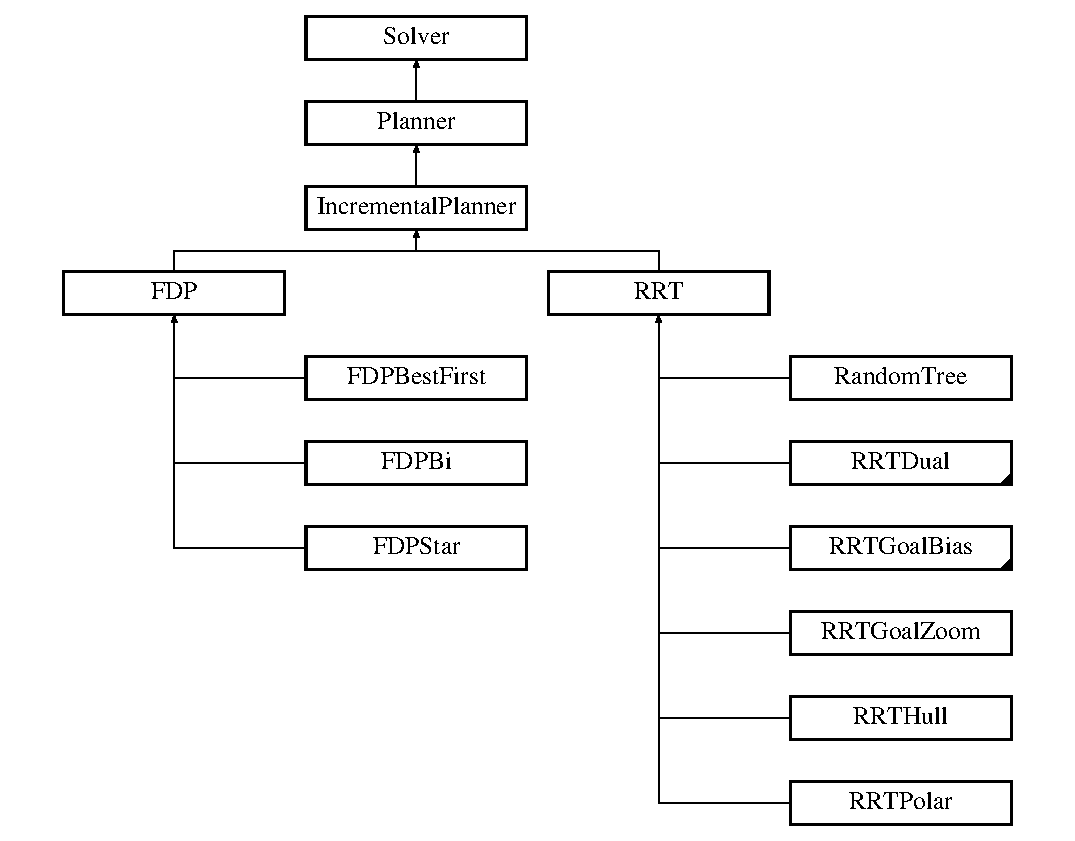
\includegraphics[height=10cm]{classIncrementalPlanner}
\end{center}
\end{figure}
\subsection*{Public Methods}
\begin{CompactItemize}
\item 
{\bf Incremental\-Planner} ({\bf Problem} $\ast$problem)
\begin{CompactList}\small\item\em A constructor that initializes data members.\item\end{CompactList}\item 
{\bf $\sim$Incremental\-Planner} ()
\item 
virtual void {\bf Construct} ()
\begin{CompactList}\small\item\em Essentially do nothing (no precomputation for incremental planners).\item\end{CompactList}\item 
void {\bf Record\-Solution} (const {\bf list}$<$ {\bf MSLNode} $\ast$$>$ \&glist, const {\bf list}$<$ {\bf MSLNode} $\ast$$>$ \&g2list)
\begin{CompactList}\small\item\em Convert a path in the graph to Path and Policy.\item\end{CompactList}\item 
void {\bf Record\-Solution} (const {\bf list}$<$ {\bf MSLNode} $\ast$$>$ \&glist)
\item 
virtual void {\bf Write\-Graphs} (ofstream \&fout)
\begin{CompactList}\small\item\em Write trees to a file.\item\end{CompactList}\item 
virtual void {\bf Read\-Graphs} (ifstream \&fin)
\begin{CompactList}\small\item\em Read trees from a file.\item\end{CompactList}\end{CompactItemize}


\subsection{Constructor \& Destructor Documentation}
\index{IncrementalPlanner@{Incremental\-Planner}!IncrementalPlanner@{IncrementalPlanner}}
\index{IncrementalPlanner@{IncrementalPlanner}!IncrementalPlanner@{Incremental\-Planner}}
\subsubsection{\setlength{\rightskip}{0pt plus 5cm}Incremental\-Planner::Incremental\-Planner ({\bf Problem} $\ast$ {\em problem})}\label{classIncrementalPlanner_a0}


A constructor that initializes data members.

\index{IncrementalPlanner@{Incremental\-Planner}!~IncrementalPlanner@{$\sim$IncrementalPlanner}}
\index{~IncrementalPlanner@{$\sim$IncrementalPlanner}!IncrementalPlanner@{Incremental\-Planner}}
\subsubsection{\setlength{\rightskip}{0pt plus 5cm}Incremental\-Planner::$\sim$Incremental\-Planner ()\hspace{0.3cm}{\tt  [inline]}}\label{classIncrementalPlanner_a1}




\subsection{Member Function Documentation}
\index{IncrementalPlanner@{Incremental\-Planner}!Construct@{Construct}}
\index{Construct@{Construct}!IncrementalPlanner@{Incremental\-Planner}}
\subsubsection{\setlength{\rightskip}{0pt plus 5cm}void Incremental\-Planner::Construct ()\hspace{0.3cm}{\tt  [virtual]}}\label{classIncrementalPlanner_a2}


Essentially do nothing (no precomputation for incremental planners).



Reimplemented from {\bf Planner} {\rm (p.\,\pageref{classPlanner_a3})}.\index{IncrementalPlanner@{Incremental\-Planner}!ReadGraphs@{ReadGraphs}}
\index{ReadGraphs@{ReadGraphs}!IncrementalPlanner@{Incremental\-Planner}}
\subsubsection{\setlength{\rightskip}{0pt plus 5cm}void Incremental\-Planner::Read\-Graphs (ifstream \& {\em fin})\hspace{0.3cm}{\tt  [virtual]}}\label{classIncrementalPlanner_a6}


Read trees from a file.



Reimplemented from {\bf Planner} {\rm (p.\,\pageref{classPlanner_a6})}.\index{IncrementalPlanner@{Incremental\-Planner}!RecordSolution@{RecordSolution}}
\index{RecordSolution@{RecordSolution}!IncrementalPlanner@{Incremental\-Planner}}
\subsubsection{\setlength{\rightskip}{0pt plus 5cm}void Incremental\-Planner::Record\-Solution (const {\bf list}$<$ {\bf MSLNode} $\ast$$>$ \& {\em glist})}\label{classIncrementalPlanner_a4}


\index{IncrementalPlanner@{Incremental\-Planner}!RecordSolution@{RecordSolution}}
\index{RecordSolution@{RecordSolution}!IncrementalPlanner@{Incremental\-Planner}}
\subsubsection{\setlength{\rightskip}{0pt plus 5cm}void Incremental\-Planner::Record\-Solution (const {\bf list}$<$ {\bf MSLNode} $\ast$$>$ \& {\em glist}, const {\bf list}$<$ {\bf MSLNode} $\ast$$>$ \& {\em g2list})}\label{classIncrementalPlanner_a3}


Convert a path in the graph to Path and Policy.

\index{IncrementalPlanner@{Incremental\-Planner}!WriteGraphs@{WriteGraphs}}
\index{WriteGraphs@{WriteGraphs}!IncrementalPlanner@{Incremental\-Planner}}
\subsubsection{\setlength{\rightskip}{0pt plus 5cm}void Incremental\-Planner::Write\-Graphs (ofstream \& {\em fout})\hspace{0.3cm}{\tt  [virtual]}}\label{classIncrementalPlanner_a5}


Write trees to a file.



Reimplemented from {\bf Planner} {\rm (p.\,\pageref{classPlanner_a5})}.

The documentation for this class was generated from the following files:\begin{CompactItemize}
\item 
{\bf planner.h}\item 
{\bf planner.C}\end{CompactItemize}

\section{list  Class Reference}
\label{classlist}\index{list@{list}}
Inheritance diagram for list::\begin{figure}[H]
\begin{center}
\leavevmode
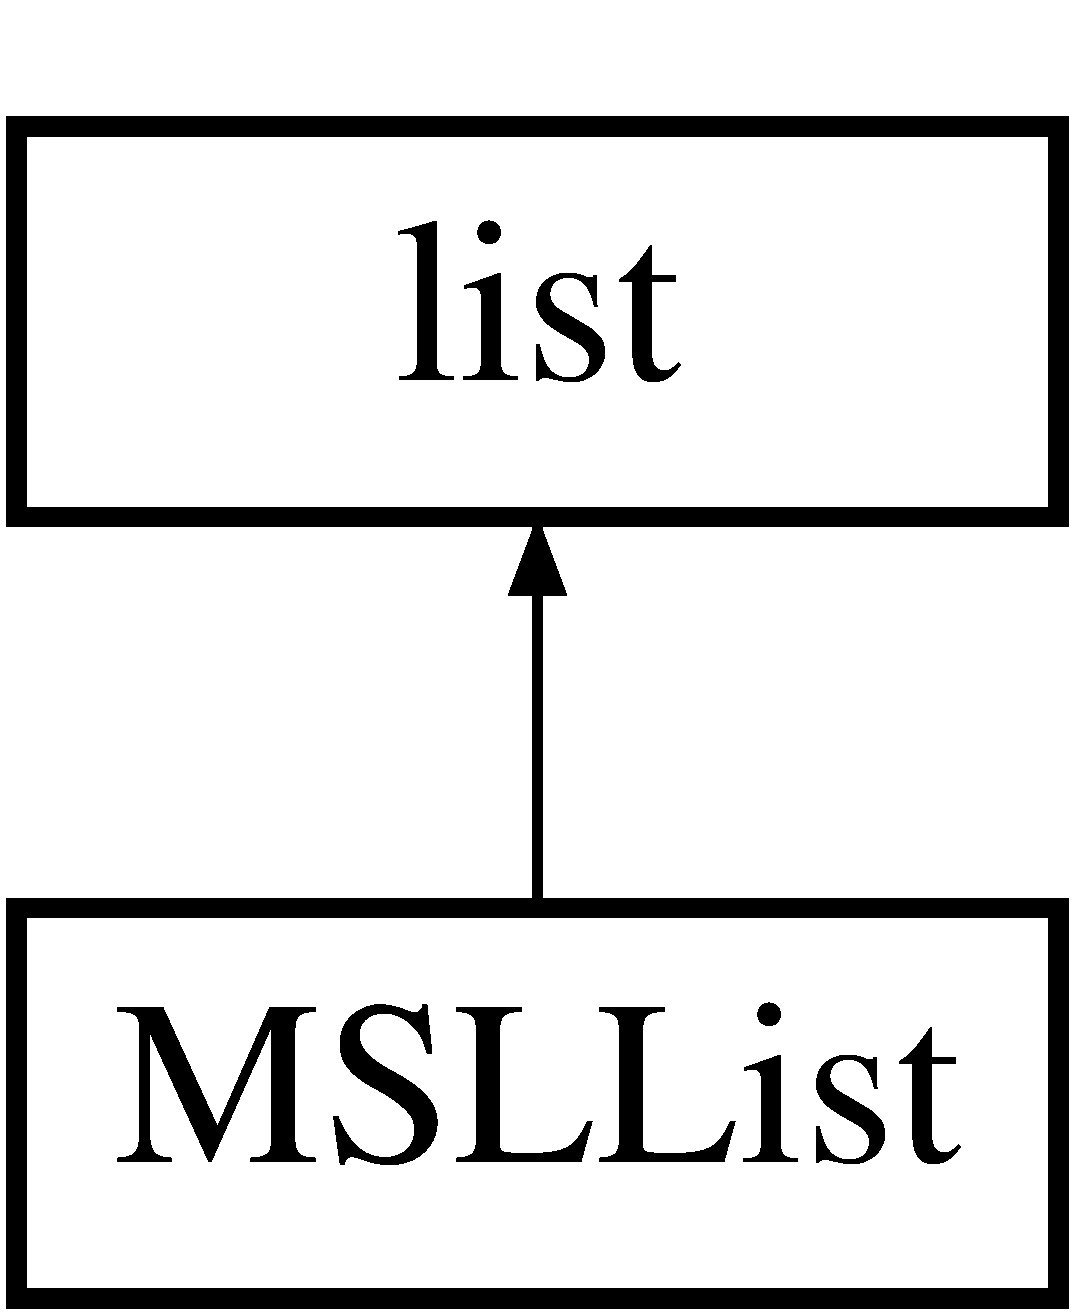
\includegraphics[height=2cm]{classlist}
\end{center}
\end{figure}


The documentation for this class was generated from the following file:\begin{CompactItemize}
\item 
{\bf msllist.h}\end{CompactItemize}

\section{Model  Class Reference}
\label{classModel}\index{Model@{Model}}
The incremental simulator model. 


{\tt \#include $<$model.h$>$}

Inheritance diagram for Model::\begin{figure}[H]
\begin{center}
\leavevmode
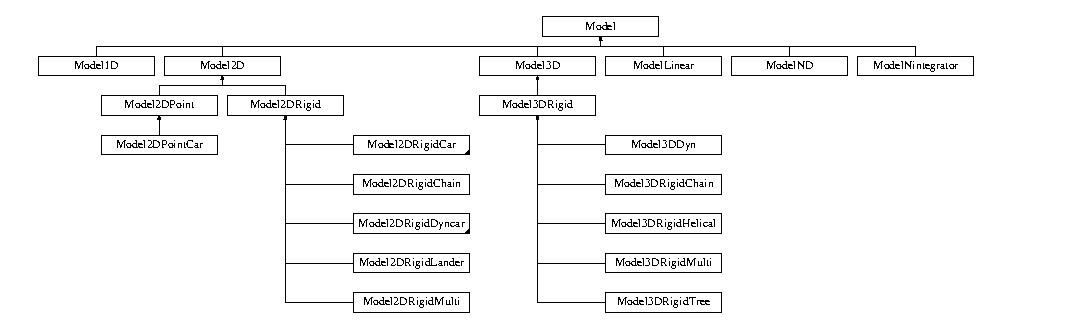
\includegraphics[height=3.97163cm]{classModel}
\end{center}
\end{figure}
\subsection*{Public Methods}
\begin{CompactItemize}
\item 
{\bf Model} (string path)
\begin{CompactList}\small\item\em Empty constructor.\item\end{CompactList}\item 
virtual {\bf $\sim$Model} ()
\begin{CompactList}\small\item\em Empty destructor.\item\end{CompactList}\item 
virtual {\bf list}$<${\bf MSLVector}$>$ {\bf Get\-Inputs} (const {\bf MSLVector} \&x)
\begin{CompactList}\small\item\em Return a {\bf list} {\rm (p.\,\pageref{classlist})} of inputs, which may depend on state.\item\end{CompactList}\item 
virtual {\bf MSLVector} {\bf State\-Transition\-Equation} (const {\bf MSLVector} \&x, const {\bf MSLVector} \&u)=0
\begin{CompactList}\small\item\em The state transition equation, or equations of motion, xdot=f(x,u).\item\end{CompactList}\item 
virtual bool {\bf Satisfied} (const {\bf MSLVector} \&x)
\begin{CompactList}\small\item\em Test whether global state-space constraints are satisfied.\item\end{CompactList}\item 
virtual {\bf MSLVector} {\bf Integrate} (const {\bf MSLVector} \&x, const {\bf MSLVector} \&u, const double \&h)=0
\begin{CompactList}\small\item\em Perform integration from state x, using input u, over time step h.\item\end{CompactList}\item 
virtual {\bf MSLVector} {\bf Linear\-Interpolate} (const {\bf MSLVector} \&x1, const {\bf MSLVector} \&x2, const double \&a)
\begin{CompactList}\small\item\em Linearly interpolate two state while respecting topology.\item\end{CompactList}\item 
virtual {\bf MSLVector} {\bf State\-Difference} (const {\bf MSLVector} \&x1, const {\bf MSLVector} \&x2)
\begin{CompactList}\small\item\em Compute a {\bf MSLVector} {\rm (p.\,\pageref{classMSLVector})} based on x2-x1. In R$^\wedge$n, the states are simply subtracted to make the {\bf MSLVector} {\rm (p.\,\pageref{classMSLVector})}. This method exists to make things work correctly for other state-space topologies.\item\end{CompactList}\item 
virtual {\bf MSLVector} {\bf State\-To\-Configuration} (const {\bf MSLVector} \&x)
\begin{CompactList}\small\item\em A method that converts a Model state in to a {\bf Geom} {\rm (p.\,\pageref{classGeom})} configuration.\item\end{CompactList}\item 
virtual double {\bf Metric} (const {\bf MSLVector} \&x1, const {\bf MSLVector} \&x2)
\begin{CompactList}\small\item\em A distance metric, which is Euclidean in the base class.\item\end{CompactList}\item 
virtual void {\bf Partialf\_\-x} (const {\bf MSLVector} \&x, const {\bf MSLVector} \&u, {\bf MSLMatrix} \&m)
\begin{CompactList}\small\item\em Partial with respect to x of the state transition equation.\item\end{CompactList}\item 
virtual void {\bf Partialf\_\-u} (const {\bf MSLVector} \&x, const {\bf MSLVector} \&u, {\bf MSLMatrix} \&m)
\begin{CompactList}\small\item\em Partial with respect to u of the state transition equation.\item\end{CompactList}\item 
virtual void {\bf L} (const {\bf MSLVector} \&x, const {\bf MSLVector} \&u, double \&l)
\begin{CompactList}\small\item\em A cost or loss function, to be used in optimization problems.\item\end{CompactList}\item 
virtual void {\bf Partial\-L\_\-x} (const {\bf MSLVector} \&x, const {\bf MSLVector} \&u, {\bf MSLMatrix} \&m)
\begin{CompactList}\small\item\em Partial of the loss with respect to x.\item\end{CompactList}\item 
virtual void {\bf Partial\-L\_\-u} (const {\bf MSLVector} \&x, const {\bf MSLVector} \&u, {\bf MSLMatrix} \&m)
\begin{CompactList}\small\item\em Partial of the loss with respect to u.\item\end{CompactList}\item 
virtual void {\bf Phi} (const {\bf MSLVector} \&x, const {\bf MSLVector} \&u, const {\bf MSLVector} \&goalstate, double \&phi)
\begin{CompactList}\small\item\em The final-state cost or loss.\item\end{CompactList}\item 
virtual void {\bf Partial\-Phi\_\-x} (const {\bf MSLVector} \&x, const {\bf MSLVector} \&u, const {\bf MSLVector} \&goalstate, {\bf MSLMatrix} \&m)
\begin{CompactList}\small\item\em Partial of the final-state loss with respect to x.\item\end{CompactList}\item 
virtual void {\bf Partial\-Phi\_\-t} (const {\bf MSLVector} \&x, const {\bf MSLVector} \&u, const {\bf MSLVector} \&goalstate, {\bf MSLMatrix} \&m)
\begin{CompactList}\small\item\em Partial of the final-state loss with respect to u.\item\end{CompactList}\item 
virtual void {\bf Psi} (const {\bf MSLVector} \&x, const {\bf MSLVector} \&goalstate, {\bf MSLVector} \&psi)
\begin{CompactList}\small\item\em An error {\bf MSLVector} {\rm (p.\,\pageref{classMSLVector})} that compares a goal state to a given state.\item\end{CompactList}\item 
virtual void {\bf Partial\-Psi\_\-x} (const {\bf MSLVector} \&x, const {\bf MSLVector} \&u, {\bf MSLMatrix} \&m)
\begin{CompactList}\small\item\em Partial of the error {\bf MSLVector} {\rm (p.\,\pageref{classMSLVector})} with respect to x.\item\end{CompactList}\item 
virtual void {\bf Partial\-Psi\_\-t} (const {\bf MSLVector} \&x, const {\bf MSLVector} \&u, {\bf MSLMatrix} \&m)
\begin{CompactList}\small\item\em Partial of the error {\bf MSLVector} {\rm (p.\,\pageref{classMSLVector})} with respect to time.\item\end{CompactList}\end{CompactItemize}
\subsection*{Public Attributes}
\begin{CompactItemize}
\item 
string {\bf File\-Path}
\begin{CompactList}\small\item\em This file path is used for all file reads.\item\end{CompactList}\item 
{\bf MSLVector} {\bf Lower\-State}
\begin{CompactList}\small\item\em {\bf MSLVector} {\rm (p.\,\pageref{classMSLVector})} of minimum values for each state variable.\item\end{CompactList}\item 
{\bf MSLVector} {\bf Upper\-State}
\begin{CompactList}\small\item\em {\bf MSLVector} {\rm (p.\,\pageref{classMSLVector})} of maximum values for each state variable.\item\end{CompactList}\item 
{\bf MSLVector} {\bf Lower\-Input}
\begin{CompactList}\small\item\em {\bf MSLVector} {\rm (p.\,\pageref{classMSLVector})} of minimum values for each input variable.\item\end{CompactList}\item 
{\bf MSLVector} {\bf Upper\-Input}
\begin{CompactList}\small\item\em {\bf MSLVector} {\rm (p.\,\pageref{classMSLVector})} of maximum values for each input variable.\item\end{CompactList}\item 
int {\bf State\-Dim}
\begin{CompactList}\small\item\em The dimension of the state space.\item\end{CompactList}\item 
int {\bf Input\-Dim}
\begin{CompactList}\small\item\em The dimension of the input space.\item\end{CompactList}\end{CompactItemize}
\subsection*{Protected Methods}
\begin{CompactItemize}
\item 
{\bf MSLVector} {\bf Runge\-Kutta\-Integrate} (const {\bf MSLVector} \&x, const {\bf MSLVector} \&u, const double \&h)
\begin{CompactList}\small\item\em Integrate xdot using 4th-order Runge-Kutta.\item\end{CompactList}\item 
{\bf MSLVector} {\bf Euler\-Integrate} (const {\bf MSLVector} \&x, const {\bf MSLVector} \&u, const double \&h)
\begin{CompactList}\small\item\em Integrate xdot using Euler integration.\item\end{CompactList}\end{CompactItemize}
\subsection*{Protected Attributes}
\begin{CompactItemize}
\item 
double {\bf Model\-Delta\-T}
\begin{CompactList}\small\item\em The time interval to use for numerical integration (affects accuracy).\item\end{CompactList}\item 
{\bf list}$<${\bf MSLVector}$>$ {\bf Inputs}
\begin{CompactList}\small\item\em The complete set of inputs.\item\end{CompactList}\end{CompactItemize}


\subsection{Detailed Description}
The incremental simulator model.

The Model classes contain incremental simulators that model the kinematics and dynamics of a variety of mechanical systems. The methods allow planning algorithms to compute the future system state, given the current state, an interval of time, and a control input applied over that interval. (The planning algorithms select the appropriate inputs using this information.) Using object-oriented class derivations, a wide variety of simulators can be included. 



\subsection{Constructor \& Destructor Documentation}
\index{Model@{Model}!Model@{Model}}
\index{Model@{Model}!Model@{Model}}
\subsubsection{\setlength{\rightskip}{0pt plus 5cm}Model::Model (string {\em path})}\label{classModel_a0}


Empty constructor.

\index{Model@{Model}!~Model@{$\sim$Model}}
\index{~Model@{$\sim$Model}!Model@{Model}}
\subsubsection{\setlength{\rightskip}{0pt plus 5cm}Model::$\sim$Model ()\hspace{0.3cm}{\tt  [inline, virtual]}}\label{classModel_a1}


Empty destructor.



\subsection{Member Function Documentation}
\index{Model@{Model}!EulerIntegrate@{EulerIntegrate}}
\index{EulerIntegrate@{EulerIntegrate}!Model@{Model}}
\subsubsection{\setlength{\rightskip}{0pt plus 5cm}{\bf MSLVector} Model::Euler\-Integrate (const {\bf MSLVector} \& {\em x}, const {\bf MSLVector} \& {\em u}, const double \& {\em h})\hspace{0.3cm}{\tt  [protected]}}\label{classModel_b1}


Integrate xdot using Euler integration.

\index{Model@{Model}!GetInputs@{GetInputs}}
\index{GetInputs@{GetInputs}!Model@{Model}}
\subsubsection{\setlength{\rightskip}{0pt plus 5cm}{\bf list}$<$ {\bf MSLVector} $>$ Model::Get\-Inputs (const {\bf MSLVector} \& {\em x})\hspace{0.3cm}{\tt  [virtual]}}\label{classModel_a2}


Return a {\bf list} {\rm (p.\,\pageref{classlist})} of inputs, which may depend on state.

\index{Model@{Model}!Integrate@{Integrate}}
\index{Integrate@{Integrate}!Model@{Model}}
\subsubsection{\setlength{\rightskip}{0pt plus 5cm}{\bf MSLVector} Model::Integrate (const {\bf MSLVector} \& {\em x}, const {\bf MSLVector} \& {\em u}, const double \& {\em h})\hspace{0.3cm}{\tt  [pure virtual]}}\label{classModel_a5}


Perform integration from state x, using input u, over time step h.



Reimplemented in {\bf Model2DPoint} {\rm (p.\,\pageref{classModel2DPoint_a2})}, {\bf Model2DPoint\-Car} {\rm (p.\,\pageref{classModel2DPointCar_a2})}, {\bf Model2DRigid} {\rm (p.\,\pageref{classModel2DRigid_a2})}, {\bf Model2DRigid\-Car\-Smooth} {\rm (p.\,\pageref{classModel2DRigidCarSmooth_a3})}, {\bf Model2DRigid\-Dyncar} {\rm (p.\,\pageref{classModel2DRigidDyncar_a2})}, {\bf Model2DRigid\-Lander} {\rm (p.\,\pageref{classModel2DRigidLander_a2})}, {\bf Model3DRigid} {\rm (p.\,\pageref{classModel3DRigid_a2})}, {\bf Model\-Car\-Dyn\-Rollover} {\rm (p.\,\pageref{classModelCarDynRollover_a5})}, {\bf Model1D} {\rm (p.\,\pageref{classModel1D_a3})}, {\bf Model\-Linear} {\rm (p.\,\pageref{classModelLinear_a3})}, {\bf Model\-ND} {\rm (p.\,\pageref{classModelND_a3})}, {\bf Model\-Nintegrator} {\rm (p.\,\pageref{classModelNintegrator_a3})}, and {\bf Model3DRigid\-Helical} {\rm (p.\,\pageref{classModel3DRigidHelical_a3})}.\index{Model@{Model}!L@{L}}
\index{L@{L}!Model@{Model}}
\subsubsection{\setlength{\rightskip}{0pt plus 5cm}void Model::L (const {\bf MSLVector} \& {\em x}, const {\bf MSLVector} \& {\em u}, double \& {\em l})\hspace{0.3cm}{\tt  [inline, virtual]}}\label{classModel_a12}


A cost or loss function, to be used in optimization problems.

\index{Model@{Model}!LinearInterpolate@{LinearInterpolate}}
\index{LinearInterpolate@{LinearInterpolate}!Model@{Model}}
\subsubsection{\setlength{\rightskip}{0pt plus 5cm}{\bf MSLVector} Model::Linear\-Interpolate (const {\bf MSLVector} \& {\em x1}, const {\bf MSLVector} \& {\em x2}, const double \& {\em a})\hspace{0.3cm}{\tt  [virtual]}}\label{classModel_a6}


Linearly interpolate two state while respecting topology.

If a=0, then x1 is returned; if a=1, then x2 is returned. All intermediate values of \$a $\backslash$in [0,1]\$ yield intermediate states. This method is defined by Model. 

Reimplemented in {\bf Model2DRigid} {\rm (p.\,\pageref{classModel2DRigid_a4})}, {\bf Model2DRigid\-Dyncar} {\rm (p.\,\pageref{classModel2DRigidDyncar_a6})}, {\bf Model2DRigid\-Multi} {\rm (p.\,\pageref{classModel2DRigidMulti_a4})}, {\bf Model2DRigid\-Chain} {\rm (p.\,\pageref{classModel2DRigidChain_a4})}, {\bf Model3DRigid} {\rm (p.\,\pageref{classModel3DRigid_a5})}, {\bf Model3DRigid\-Multi} {\rm (p.\,\pageref{classModel3DRigidMulti_a3})}, {\bf Model3DRigid\-Chain} {\rm (p.\,\pageref{classModel3DRigidChain_a4})}, {\bf Model3DRigid\-Tree} {\rm (p.\,\pageref{classModel3DRigidTree_a4})}, and {\bf Model\-Car\-Dyn\-Smooth\-Rollover} {\rm (p.\,\pageref{classModelCarDynSmoothRollover_a5})}.\index{Model@{Model}!Metric@{Metric}}
\index{Metric@{Metric}!Model@{Model}}
\subsubsection{\setlength{\rightskip}{0pt plus 5cm}double Model::Metric (const {\bf MSLVector} \& {\em x1}, const {\bf MSLVector} \& {\em x2})\hspace{0.3cm}{\tt  [virtual]}}\label{classModel_a9}


A distance metric, which is Euclidean in the base class.



Reimplemented in {\bf Model2DPoint} {\rm (p.\,\pageref{classModel2DPoint_a4})}, {\bf Model2DPoint\-Car} {\rm (p.\,\pageref{classModel2DPointCar_a4})}, {\bf Model2DRigid} {\rm (p.\,\pageref{classModel2DRigid_a5})}, {\bf Model2DRigid\-Car\-Smooth} {\rm (p.\,\pageref{classModel2DRigidCarSmooth_a4})}, {\bf Model2DRigid\-Car\-Smooth\-Trailer} {\rm (p.\,\pageref{classModel2DRigidCarSmoothTrailer_a3})}, {\bf Model2DRigid\-Car\-Smooth2Trailers} {\rm (p.\,\pageref{classModel2DRigidCarSmooth2Trailers_a3})}, {\bf Model2DRigid\-Car\-Smooth3Trailers} {\rm (p.\,\pageref{classModel2DRigidCarSmooth3Trailers_a3})}, {\bf Model2DRigid\-Dyncar} {\rm (p.\,\pageref{classModel2DRigidDyncar_a5})}, {\bf Model2DRigid\-Lander} {\rm (p.\,\pageref{classModel2DRigidLander_a5})}, {\bf Model2DRigid\-Multi} {\rm (p.\,\pageref{classModel2DRigidMulti_a2})}, {\bf Model2DRigid\-Chain} {\rm (p.\,\pageref{classModel2DRigidChain_a5})}, {\bf Model3DRigid} {\rm (p.\,\pageref{classModel3DRigid_a4})}, {\bf Model3DRigid\-Multi} {\rm (p.\,\pageref{classModel3DRigidMulti_a2})}, {\bf Model3DRigid\-Chain} {\rm (p.\,\pageref{classModel3DRigidChain_a5})}, {\bf Model3DRigid\-Tree} {\rm (p.\,\pageref{classModel3DRigidTree_a5})}, {\bf Model\-Car\-Dyn} {\rm (p.\,\pageref{classModelCarDyn_a3})}, {\bf Model\-Car\-Dyn\-Ntire} {\rm (p.\,\pageref{classModelCarDynNtire_a3})}, {\bf Model\-Car\-Dyn\-Rollover} {\rm (p.\,\pageref{classModelCarDynRollover_a6})}, {\bf Model\-Car\-Dyn\-Smooth\-Rollover} {\rm (p.\,\pageref{classModelCarDynSmoothRollover_a4})}, and {\bf Model1D} {\rm (p.\,\pageref{classModel1D_a5})}.\index{Model@{Model}!PartialL_u@{PartialL\_\-u}}
\index{PartialL_u@{PartialL\_\-u}!Model@{Model}}
\subsubsection{\setlength{\rightskip}{0pt plus 5cm}void Model::Partial\-L\_\-u (const {\bf MSLVector} \& {\em x}, const {\bf MSLVector} \& {\em u}, {\bf MSLMatrix} \& {\em m})\hspace{0.3cm}{\tt  [inline, virtual]}}\label{classModel_a14}


Partial of the loss with respect to u.

\index{Model@{Model}!PartialL_x@{PartialL\_\-x}}
\index{PartialL_x@{PartialL\_\-x}!Model@{Model}}
\subsubsection{\setlength{\rightskip}{0pt plus 5cm}void Model::Partial\-L\_\-x (const {\bf MSLVector} \& {\em x}, const {\bf MSLVector} \& {\em u}, {\bf MSLMatrix} \& {\em m})\hspace{0.3cm}{\tt  [inline, virtual]}}\label{classModel_a13}


Partial of the loss with respect to x.

\index{Model@{Model}!PartialPhi_t@{PartialPhi\_\-t}}
\index{PartialPhi_t@{PartialPhi\_\-t}!Model@{Model}}
\subsubsection{\setlength{\rightskip}{0pt plus 5cm}void Model::Partial\-Phi\_\-t (const {\bf MSLVector} \& {\em x}, const {\bf MSLVector} \& {\em u}, const {\bf MSLVector} \& {\em goalstate}, {\bf MSLMatrix} \& {\em m})\hspace{0.3cm}{\tt  [inline, virtual]}}\label{classModel_a17}


Partial of the final-state loss with respect to u.

\index{Model@{Model}!PartialPhi_x@{PartialPhi\_\-x}}
\index{PartialPhi_x@{PartialPhi\_\-x}!Model@{Model}}
\subsubsection{\setlength{\rightskip}{0pt plus 5cm}void Model::Partial\-Phi\_\-x (const {\bf MSLVector} \& {\em x}, const {\bf MSLVector} \& {\em u}, const {\bf MSLVector} \& {\em goalstate}, {\bf MSLMatrix} \& {\em m})\hspace{0.3cm}{\tt  [inline, virtual]}}\label{classModel_a16}


Partial of the final-state loss with respect to x.

\index{Model@{Model}!PartialPsi_t@{PartialPsi\_\-t}}
\index{PartialPsi_t@{PartialPsi\_\-t}!Model@{Model}}
\subsubsection{\setlength{\rightskip}{0pt plus 5cm}void Model::Partial\-Psi\_\-t (const {\bf MSLVector} \& {\em x}, const {\bf MSLVector} \& {\em u}, {\bf MSLMatrix} \& {\em m})\hspace{0.3cm}{\tt  [inline, virtual]}}\label{classModel_a20}


Partial of the error {\bf MSLVector} {\rm (p.\,\pageref{classMSLVector})} with respect to time.

\index{Model@{Model}!PartialPsi_x@{PartialPsi\_\-x}}
\index{PartialPsi_x@{PartialPsi\_\-x}!Model@{Model}}
\subsubsection{\setlength{\rightskip}{0pt plus 5cm}void Model::Partial\-Psi\_\-x (const {\bf MSLVector} \& {\em x}, const {\bf MSLVector} \& {\em u}, {\bf MSLMatrix} \& {\em m})\hspace{0.3cm}{\tt  [inline, virtual]}}\label{classModel_a19}


Partial of the error {\bf MSLVector} {\rm (p.\,\pageref{classMSLVector})} with respect to x.

\index{Model@{Model}!Partialf_u@{Partialf\_\-u}}
\index{Partialf_u@{Partialf\_\-u}!Model@{Model}}
\subsubsection{\setlength{\rightskip}{0pt plus 5cm}void Model::Partialf\_\-u (const {\bf MSLVector} \& {\em x}, const {\bf MSLVector} \& {\em u}, {\bf MSLMatrix} \& {\em m})\hspace{0.3cm}{\tt  [inline, virtual]}}\label{classModel_a11}


Partial with respect to u of the state transition equation.

\index{Model@{Model}!Partialf_x@{Partialf\_\-x}}
\index{Partialf_x@{Partialf\_\-x}!Model@{Model}}
\subsubsection{\setlength{\rightskip}{0pt plus 5cm}void Model::Partialf\_\-x (const {\bf MSLVector} \& {\em x}, const {\bf MSLVector} \& {\em u}, {\bf MSLMatrix} \& {\em m})\hspace{0.3cm}{\tt  [inline, virtual]}}\label{classModel_a10}


Partial with respect to x of the state transition equation.

\index{Model@{Model}!Phi@{Phi}}
\index{Phi@{Phi}!Model@{Model}}
\subsubsection{\setlength{\rightskip}{0pt plus 5cm}void Model::Phi (const {\bf MSLVector} \& {\em x}, const {\bf MSLVector} \& {\em u}, const {\bf MSLVector} \& {\em goalstate}, double \& {\em phi})\hspace{0.3cm}{\tt  [inline, virtual]}}\label{classModel_a15}


The final-state cost or loss.

\index{Model@{Model}!Psi@{Psi}}
\index{Psi@{Psi}!Model@{Model}}
\subsubsection{\setlength{\rightskip}{0pt plus 5cm}void Model::Psi (const {\bf MSLVector} \& {\em x}, const {\bf MSLVector} \& {\em goalstate}, {\bf MSLVector} \& {\em psi})\hspace{0.3cm}{\tt  [inline, virtual]}}\label{classModel_a18}


An error {\bf MSLVector} {\rm (p.\,\pageref{classMSLVector})} that compares a goal state to a given state.

\index{Model@{Model}!RungeKuttaIntegrate@{RungeKuttaIntegrate}}
\index{RungeKuttaIntegrate@{RungeKuttaIntegrate}!Model@{Model}}
\subsubsection{\setlength{\rightskip}{0pt plus 5cm}{\bf MSLVector} Model::Runge\-Kutta\-Integrate (const {\bf MSLVector} \& {\em x}, const {\bf MSLVector} \& {\em u}, const double \& {\em h})\hspace{0.3cm}{\tt  [protected]}}\label{classModel_b0}


Integrate xdot using 4th-order Runge-Kutta.

\index{Model@{Model}!Satisfied@{Satisfied}}
\index{Satisfied@{Satisfied}!Model@{Model}}
\subsubsection{\setlength{\rightskip}{0pt plus 5cm}bool Model::Satisfied (const {\bf MSLVector} \& {\em x})\hspace{0.3cm}{\tt  [virtual]}}\label{classModel_a4}


Test whether global state-space constraints are satisfied.



Reimplemented in {\bf Model2DRigid\-Car\-Smooth} {\rm (p.\,\pageref{classModel2DRigidCarSmooth_a6})}, {\bf Model2DRigid\-Car\-Smooth\-Trailer} {\rm (p.\,\pageref{classModel2DRigidCarSmoothTrailer_a5})}, {\bf Model2DRigid\-Car\-Smooth2Trailers} {\rm (p.\,\pageref{classModel2DRigidCarSmooth2Trailers_a5})}, {\bf Model2DRigid\-Car\-Smooth3Trailers} {\rm (p.\,\pageref{classModel2DRigidCarSmooth3Trailers_a5})}, {\bf Model2DRigid\-Chain} {\rm (p.\,\pageref{classModel2DRigidChain_a6})}, {\bf Model3DRigid\-Chain} {\rm (p.\,\pageref{classModel3DRigidChain_a6})}, {\bf Model3DRigid\-Tree} {\rm (p.\,\pageref{classModel3DRigidTree_a6})}, {\bf Model3DDyn} {\rm (p.\,\pageref{classModel3DDyn_a3})}, {\bf Model\-Car} {\rm (p.\,\pageref{classModelCar_a3})}, and {\bf Model\-Car\-Dyn\-Rollover} {\rm (p.\,\pageref{classModelCarDynRollover_a8})}.\index{Model@{Model}!StateDifference@{StateDifference}}
\index{StateDifference@{StateDifference}!Model@{Model}}
\subsubsection{\setlength{\rightskip}{0pt plus 5cm}{\bf MSLVector} Model::State\-Difference (const {\bf MSLVector} \& {\em x1}, const {\bf MSLVector} \& {\em x2})\hspace{0.3cm}{\tt  [virtual]}}\label{classModel_a7}


Compute a {\bf MSLVector} {\rm (p.\,\pageref{classMSLVector})} based on x2-x1. In R$^\wedge$n, the states are simply subtracted to make the {\bf MSLVector} {\rm (p.\,\pageref{classMSLVector})}. This method exists to make things work correctly for other state-space topologies.

\index{Model@{Model}!StateToConfiguration@{StateToConfiguration}}
\index{StateToConfiguration@{StateToConfiguration}!Model@{Model}}
\subsubsection{\setlength{\rightskip}{0pt plus 5cm}{\bf MSLVector} Model::State\-To\-Configuration (const {\bf MSLVector} \& {\em x})\hspace{0.3cm}{\tt  [virtual]}}\label{classModel_a8}


A method that converts a Model state in to a {\bf Geom} {\rm (p.\,\pageref{classGeom})} configuration.



Reimplemented in {\bf Model2D} {\rm (p.\,\pageref{classModel2D_a2})}, {\bf Model2DRigid} {\rm (p.\,\pageref{classModel2DRigid_a6})}, {\bf Model2DRigid\-Car\-Smooth} {\rm (p.\,\pageref{classModel2DRigidCarSmooth_a5})}, {\bf Model2DRigid\-Car\-Smooth\-Trailer} {\rm (p.\,\pageref{classModel2DRigidCarSmoothTrailer_a4})}, {\bf Model2DRigid\-Car\-Smooth2Trailers} {\rm (p.\,\pageref{classModel2DRigidCarSmooth2Trailers_a4})}, {\bf Model2DRigid\-Car\-Smooth3Trailers} {\rm (p.\,\pageref{classModel2DRigidCarSmooth3Trailers_a4})}, {\bf Model2DRigid\-Dyncar} {\rm (p.\,\pageref{classModel2DRigidDyncar_a3})}, {\bf Model2DRigid\-Lander} {\rm (p.\,\pageref{classModel2DRigidLander_a3})}, {\bf Model2DRigid\-Multi} {\rm (p.\,\pageref{classModel2DRigidMulti_a3})}, {\bf Model2DRigid\-Chain} {\rm (p.\,\pageref{classModel2DRigidChain_a2})}, {\bf Model3DRigid\-Chain} {\rm (p.\,\pageref{classModel3DRigidChain_a3})}, {\bf Model3DRigid\-Tree} {\rm (p.\,\pageref{classModel3DRigidTree_a3})}, {\bf Model\-Car} {\rm (p.\,\pageref{classModelCar_a2})}, {\bf Model\-Car\-Smooth} {\rm (p.\,\pageref{classModelCarSmooth_a2})}, {\bf Model\-Car\-Dyn} {\rm (p.\,\pageref{classModelCarDyn_a2})}, {\bf Model\-Car\-Dyn\-Ntire} {\rm (p.\,\pageref{classModelCarDynNtire_a2})}, {\bf Model\-Car\-Dyn\-Rollover} {\rm (p.\,\pageref{classModelCarDynRollover_a4})}, {\bf Model\-Car\-Dyn\-Smooth\-Rollover} {\rm (p.\,\pageref{classModelCarDynSmoothRollover_a3})}, {\bf Model1D} {\rm (p.\,\pageref{classModel1D_a2})}, {\bf Model\-Linear} {\rm (p.\,\pageref{classModelLinear_a2})}, {\bf Model\-ND} {\rm (p.\,\pageref{classModelND_a2})}, and {\bf Model\-Nintegrator} {\rm (p.\,\pageref{classModelNintegrator_a2})}.\index{Model@{Model}!StateTransitionEquation@{StateTransitionEquation}}
\index{StateTransitionEquation@{StateTransitionEquation}!Model@{Model}}
\subsubsection{\setlength{\rightskip}{0pt plus 5cm}{\bf MSLVector} Model::State\-Transition\-Equation (const {\bf MSLVector} \& {\em x}, const {\bf MSLVector} \& {\em u})\hspace{0.3cm}{\tt  [pure virtual]}}\label{classModel_a3}


The state transition equation, or equations of motion, xdot=f(x,u).



Reimplemented in {\bf Model2DPoint} {\rm (p.\,\pageref{classModel2DPoint_a3})}, {\bf Model2DPoint\-Car} {\rm (p.\,\pageref{classModel2DPointCar_a3})}, {\bf Model2DRigid} {\rm (p.\,\pageref{classModel2DRigid_a3})}, {\bf Model2DRigid\-Car} {\rm (p.\,\pageref{classModel2DRigidCar_a2})}, {\bf Model2DRigid\-Car\-Smooth} {\rm (p.\,\pageref{classModel2DRigidCarSmooth_a2})}, {\bf Model2DRigid\-Car\-Smooth\-Trailer} {\rm (p.\,\pageref{classModel2DRigidCarSmoothTrailer_a2})}, {\bf Model2DRigid\-Car\-Smooth2Trailers} {\rm (p.\,\pageref{classModel2DRigidCarSmooth2Trailers_a2})}, {\bf Model2DRigid\-Car\-Smooth3Trailers} {\rm (p.\,\pageref{classModel2DRigidCarSmooth3Trailers_a2})}, {\bf Model2DRigid\-Dyncar} {\rm (p.\,\pageref{classModel2DRigidDyncar_a4})}, {\bf Model2DRigid\-Dyncar\-Ntire} {\rm (p.\,\pageref{classModel2DRigidDyncarNtire_a2})}, {\bf Model2DRigid\-Lander} {\rm (p.\,\pageref{classModel2DRigidLander_a4})}, {\bf Model2DRigid\-Chain} {\rm (p.\,\pageref{classModel2DRigidChain_a3})}, {\bf Model3DRigid} {\rm (p.\,\pageref{classModel3DRigid_a3})}, {\bf Model3DRigid\-Chain} {\rm (p.\,\pageref{classModel3DRigidChain_a2})}, {\bf Model3DRigid\-Tree} {\rm (p.\,\pageref{classModel3DRigidTree_a2})}, {\bf Model3DDyn} {\rm (p.\,\pageref{classModel3DDyn_a2})}, {\bf Model\-Car\-Dyn\-Rollover} {\rm (p.\,\pageref{classModelCarDynRollover_a3})}, {\bf Model\-Car\-Dyn\-Smooth\-Rollover} {\rm (p.\,\pageref{classModelCarDynSmoothRollover_a2})}, {\bf Model1D} {\rm (p.\,\pageref{classModel1D_a4})}, {\bf Model\-Linear} {\rm (p.\,\pageref{classModelLinear_a4})}, {\bf Model\-ND} {\rm (p.\,\pageref{classModelND_a4})}, {\bf Model\-Nintegrator} {\rm (p.\,\pageref{classModelNintegrator_a4})}, and {\bf Model3DRigid\-Helical} {\rm (p.\,\pageref{classModel3DRigidHelical_a2})}.

\subsection{Member Data Documentation}
\index{Model@{Model}!FilePath@{FilePath}}
\index{FilePath@{FilePath}!Model@{Model}}
\subsubsection{\setlength{\rightskip}{0pt plus 5cm}string Model::File\-Path}\label{classModel_m0}


This file path is used for all file reads.

\index{Model@{Model}!InputDim@{InputDim}}
\index{InputDim@{InputDim}!Model@{Model}}
\subsubsection{\setlength{\rightskip}{0pt plus 5cm}int Model::Input\-Dim}\label{classModel_m6}


The dimension of the input space.

\index{Model@{Model}!Inputs@{Inputs}}
\index{Inputs@{Inputs}!Model@{Model}}
\subsubsection{\setlength{\rightskip}{0pt plus 5cm}{\bf list}$<$ {\bf MSLVector} $>$ Model::Inputs\hspace{0.3cm}{\tt  [protected]}}\label{classModel_n1}


The complete set of inputs.

\index{Model@{Model}!LowerInput@{LowerInput}}
\index{LowerInput@{LowerInput}!Model@{Model}}
\subsubsection{\setlength{\rightskip}{0pt plus 5cm}{\bf MSLVector} Model::Lower\-Input}\label{classModel_m3}


{\bf MSLVector} {\rm (p.\,\pageref{classMSLVector})} of minimum values for each input variable.

\index{Model@{Model}!LowerState@{LowerState}}
\index{LowerState@{LowerState}!Model@{Model}}
\subsubsection{\setlength{\rightskip}{0pt plus 5cm}{\bf MSLVector} Model::Lower\-State}\label{classModel_m1}


{\bf MSLVector} {\rm (p.\,\pageref{classMSLVector})} of minimum values for each state variable.

\index{Model@{Model}!ModelDeltaT@{ModelDeltaT}}
\index{ModelDeltaT@{ModelDeltaT}!Model@{Model}}
\subsubsection{\setlength{\rightskip}{0pt plus 5cm}double Model::Model\-Delta\-T\hspace{0.3cm}{\tt  [protected]}}\label{classModel_n0}


The time interval to use for numerical integration (affects accuracy).

\index{Model@{Model}!StateDim@{StateDim}}
\index{StateDim@{StateDim}!Model@{Model}}
\subsubsection{\setlength{\rightskip}{0pt plus 5cm}int Model::State\-Dim}\label{classModel_m5}


The dimension of the state space.

\index{Model@{Model}!UpperInput@{UpperInput}}
\index{UpperInput@{UpperInput}!Model@{Model}}
\subsubsection{\setlength{\rightskip}{0pt plus 5cm}{\bf MSLVector} Model::Upper\-Input}\label{classModel_m4}


{\bf MSLVector} {\rm (p.\,\pageref{classMSLVector})} of maximum values for each input variable.

\index{Model@{Model}!UpperState@{UpperState}}
\index{UpperState@{UpperState}!Model@{Model}}
\subsubsection{\setlength{\rightskip}{0pt plus 5cm}{\bf MSLVector} Model::Upper\-State}\label{classModel_m2}


{\bf MSLVector} {\rm (p.\,\pageref{classMSLVector})} of maximum values for each state variable.



The documentation for this class was generated from the following files:\begin{CompactItemize}
\item 
{\bf model.h}\item 
{\bf model.C}\end{CompactItemize}

\section{Model1D  Class Reference}
\label{classModel1D}\index{Model1D@{Model1D}}
A simple one-dimensional model for dynamics studies. 


{\tt \#include $<$modelmisc.h$>$}

Inheritance diagram for Model1D::\begin{figure}[H]
\begin{center}
\leavevmode
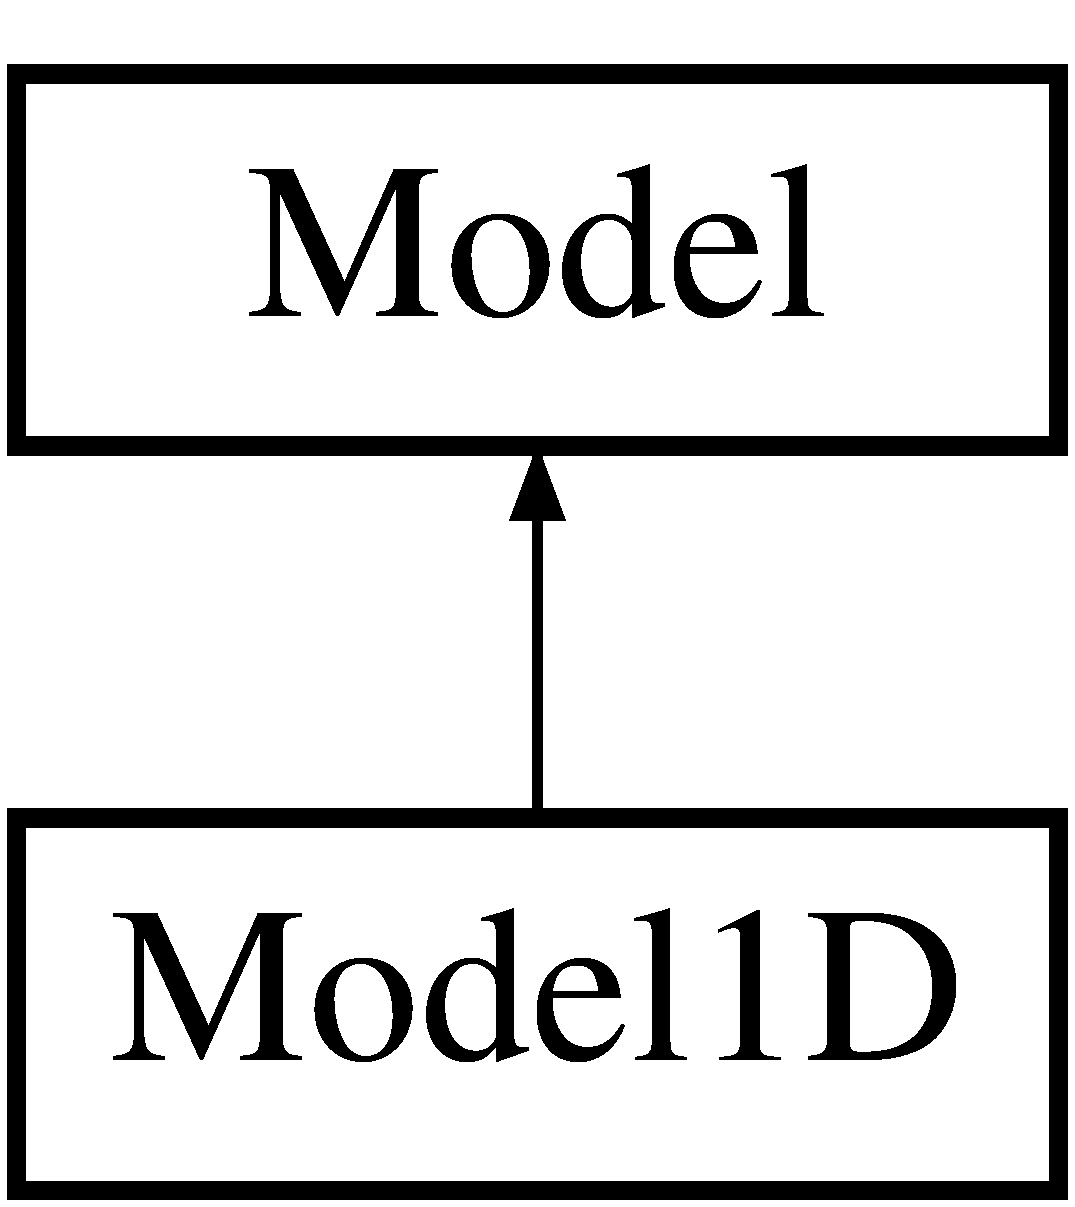
\includegraphics[height=2cm]{classModel1D}
\end{center}
\end{figure}
\subsection*{Public Methods}
\begin{CompactItemize}
\item 
{\bf Model1D} (string path)
\item 
virtual {\bf $\sim$Model1D} ()
\item 
virtual {\bf MSLVector} {\bf State\-To\-Configuration} (const {\bf MSLVector} \&x)
\begin{CompactList}\small\item\em A method that converts a {\bf Model} {\rm (p.\,\pageref{classModel})} state in to a {\bf Geom} {\rm (p.\,\pageref{classGeom})} configuration.\item\end{CompactList}\item 
virtual {\bf MSLVector} {\bf Integrate} (const {\bf MSLVector} \&x, const {\bf MSLVector} \&u, const double \&h)
\begin{CompactList}\small\item\em Perform integration from state x, using input u, over time step h.\item\end{CompactList}\item 
virtual {\bf MSLVector} {\bf State\-Transition\-Equation} (const {\bf MSLVector} \&x, const {\bf MSLVector} \&u)
\begin{CompactList}\small\item\em The state transition equation, or equations of motion, xdot=f(x,u).\item\end{CompactList}\item 
virtual double {\bf Metric} (const {\bf MSLVector} \&x1, const {\bf MSLVector} \&x2)
\begin{CompactList}\small\item\em A distance metric, which is Euclidean in the base class.\item\end{CompactList}\end{CompactItemize}
\subsection*{Public Attributes}
\begin{CompactItemize}
\item 
double {\bf Force}
\end{CompactItemize}


\subsection{Detailed Description}
A simple one-dimensional model for dynamics studies.



\subsection{Constructor \& Destructor Documentation}
\index{Model1D@{Model1D}!Model1D@{Model1D}}
\index{Model1D@{Model1D}!Model1D@{Model1D}}
\subsubsection{\setlength{\rightskip}{0pt plus 5cm}Model1D::Model1D (string {\em path} = \char`\"{}\char`\"{})}\label{classModel1D_a0}


\index{Model1D@{Model1D}!~Model1D@{$\sim$Model1D}}
\index{~Model1D@{$\sim$Model1D}!Model1D@{Model1D}}
\subsubsection{\setlength{\rightskip}{0pt plus 5cm}Model1D::$\sim$Model1D ()\hspace{0.3cm}{\tt  [inline, virtual]}}\label{classModel1D_a1}




\subsection{Member Function Documentation}
\index{Model1D@{Model1D}!Integrate@{Integrate}}
\index{Integrate@{Integrate}!Model1D@{Model1D}}
\subsubsection{\setlength{\rightskip}{0pt plus 5cm}{\bf MSLVector} Model1D::Integrate (const {\bf MSLVector} \& {\em x}, const {\bf MSLVector} \& {\em u}, const double \& {\em h})\hspace{0.3cm}{\tt  [virtual]}}\label{classModel1D_a3}


Perform integration from state x, using input u, over time step h.



Reimplemented from {\bf Model} {\rm (p.\,\pageref{classModel_a5})}.\index{Model1D@{Model1D}!Metric@{Metric}}
\index{Metric@{Metric}!Model1D@{Model1D}}
\subsubsection{\setlength{\rightskip}{0pt plus 5cm}double Model1D::Metric (const {\bf MSLVector} \& {\em x1}, const {\bf MSLVector} \& {\em x2})\hspace{0.3cm}{\tt  [virtual]}}\label{classModel1D_a5}


A distance metric, which is Euclidean in the base class.



Reimplemented from {\bf Model} {\rm (p.\,\pageref{classModel_a9})}.\index{Model1D@{Model1D}!StateToConfiguration@{StateToConfiguration}}
\index{StateToConfiguration@{StateToConfiguration}!Model1D@{Model1D}}
\subsubsection{\setlength{\rightskip}{0pt plus 5cm}{\bf MSLVector} Model1D::State\-To\-Configuration (const {\bf MSLVector} \& {\em x})\hspace{0.3cm}{\tt  [virtual]}}\label{classModel1D_a2}


A method that converts a {\bf Model} {\rm (p.\,\pageref{classModel})} state in to a {\bf Geom} {\rm (p.\,\pageref{classGeom})} configuration.



Reimplemented from {\bf Model} {\rm (p.\,\pageref{classModel_a8})}.\index{Model1D@{Model1D}!StateTransitionEquation@{StateTransitionEquation}}
\index{StateTransitionEquation@{StateTransitionEquation}!Model1D@{Model1D}}
\subsubsection{\setlength{\rightskip}{0pt plus 5cm}{\bf MSLVector} Model1D::State\-Transition\-Equation (const {\bf MSLVector} \& {\em x}, const {\bf MSLVector} \& {\em u})\hspace{0.3cm}{\tt  [virtual]}}\label{classModel1D_a4}


The state transition equation, or equations of motion, xdot=f(x,u).



Reimplemented from {\bf Model} {\rm (p.\,\pageref{classModel_a3})}.

\subsection{Member Data Documentation}
\index{Model1D@{Model1D}!Force@{Force}}
\index{Force@{Force}!Model1D@{Model1D}}
\subsubsection{\setlength{\rightskip}{0pt plus 5cm}double Model1D::Force}\label{classModel1D_m0}




The documentation for this class was generated from the following files:\begin{CompactItemize}
\item 
{\bf modelmisc.h}\item 
{\bf modelmisc.C}\end{CompactItemize}

\section{Model2D  Class Reference}
\label{classModel2D}\index{Model2D@{Model2D}}
Base for all 2D models. 


{\tt \#include $<$model2d.h$>$}

Inheritance diagram for Model2D::\begin{figure}[H]
\begin{center}
\leavevmode
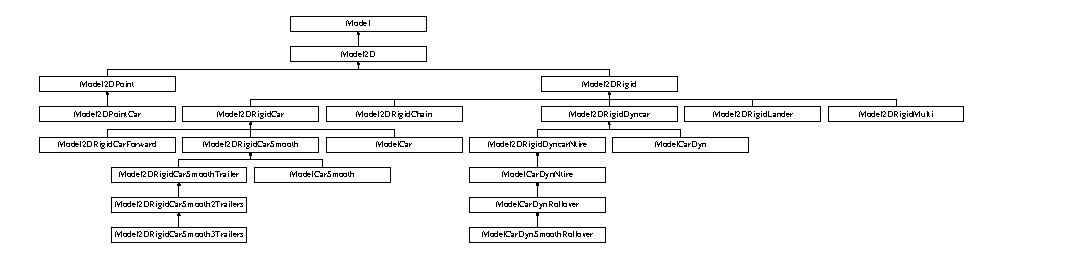
\includegraphics[height=3.03318cm]{classModel2D}
\end{center}
\end{figure}
\subsection*{Public Methods}
\begin{CompactItemize}
\item 
{\bf Model2D} (string path)
\item 
virtual {\bf $\sim$Model2D} ()
\item 
virtual {\bf MSLVector} {\bf State\-To\-Configuration} (const {\bf MSLVector} \&x)
\begin{CompactList}\small\item\em A method that converts a {\bf Model} {\rm (p.\,\pageref{classModel})} state in to a {\bf Geom} {\rm (p.\,\pageref{classGeom})} configuration.\item\end{CompactList}\end{CompactItemize}


\subsection{Detailed Description}
Base for all 2D models.



\subsection{Constructor \& Destructor Documentation}
\index{Model2D@{Model2D}!Model2D@{Model2D}}
\index{Model2D@{Model2D}!Model2D@{Model2D}}
\subsubsection{\setlength{\rightskip}{0pt plus 5cm}Model2D::Model2D (string {\em path} = \char`\"{}\char`\"{})}\label{classModel2D_a0}


\index{Model2D@{Model2D}!~Model2D@{$\sim$Model2D}}
\index{~Model2D@{$\sim$Model2D}!Model2D@{Model2D}}
\subsubsection{\setlength{\rightskip}{0pt plus 5cm}Model2D::$\sim$Model2D ()\hspace{0.3cm}{\tt  [inline, virtual]}}\label{classModel2D_a1}




\subsection{Member Function Documentation}
\index{Model2D@{Model2D}!StateToConfiguration@{StateToConfiguration}}
\index{StateToConfiguration@{StateToConfiguration}!Model2D@{Model2D}}
\subsubsection{\setlength{\rightskip}{0pt plus 5cm}{\bf MSLVector} Model2D::State\-To\-Configuration (const {\bf MSLVector} \& {\em x})\hspace{0.3cm}{\tt  [virtual]}}\label{classModel2D_a2}


A method that converts a {\bf Model} {\rm (p.\,\pageref{classModel})} state in to a {\bf Geom} {\rm (p.\,\pageref{classGeom})} configuration.



Reimplemented from {\bf Model} {\rm (p.\,\pageref{classModel_a8})}.

Reimplemented in {\bf Model2DRigid} {\rm (p.\,\pageref{classModel2DRigid_a6})}, {\bf Model2DRigid\-Car\-Smooth} {\rm (p.\,\pageref{classModel2DRigidCarSmooth_a5})}, {\bf Model2DRigid\-Car\-Smooth\-Trailer} {\rm (p.\,\pageref{classModel2DRigidCarSmoothTrailer_a4})}, {\bf Model2DRigid\-Car\-Smooth2Trailers} {\rm (p.\,\pageref{classModel2DRigidCarSmooth2Trailers_a4})}, {\bf Model2DRigid\-Car\-Smooth3Trailers} {\rm (p.\,\pageref{classModel2DRigidCarSmooth3Trailers_a4})}, {\bf Model2DRigid\-Dyncar} {\rm (p.\,\pageref{classModel2DRigidDyncar_a3})}, {\bf Model2DRigid\-Lander} {\rm (p.\,\pageref{classModel2DRigidLander_a3})}, {\bf Model2DRigid\-Multi} {\rm (p.\,\pageref{classModel2DRigidMulti_a3})}, {\bf Model2DRigid\-Chain} {\rm (p.\,\pageref{classModel2DRigidChain_a2})}, {\bf Model\-Car} {\rm (p.\,\pageref{classModelCar_a2})}, {\bf Model\-Car\-Smooth} {\rm (p.\,\pageref{classModelCarSmooth_a2})}, {\bf Model\-Car\-Dyn} {\rm (p.\,\pageref{classModelCarDyn_a2})}, {\bf Model\-Car\-Dyn\-Ntire} {\rm (p.\,\pageref{classModelCarDynNtire_a2})}, {\bf Model\-Car\-Dyn\-Rollover} {\rm (p.\,\pageref{classModelCarDynRollover_a4})}, and {\bf Model\-Car\-Dyn\-Smooth\-Rollover} {\rm (p.\,\pageref{classModelCarDynSmoothRollover_a3})}.

The documentation for this class was generated from the following files:\begin{CompactItemize}
\item 
{\bf model2d.h}\item 
{\bf model2d.C}\end{CompactItemize}

\section{Model2DPoint  Class Reference}
\label{classModel2DPoint}\index{Model2DPoint@{Model2DPoint}}
A point robot in a 2D world. 


{\tt \#include $<$model2d.h$>$}

Inheritance diagram for Model2DPoint::\begin{figure}[H]
\begin{center}
\leavevmode
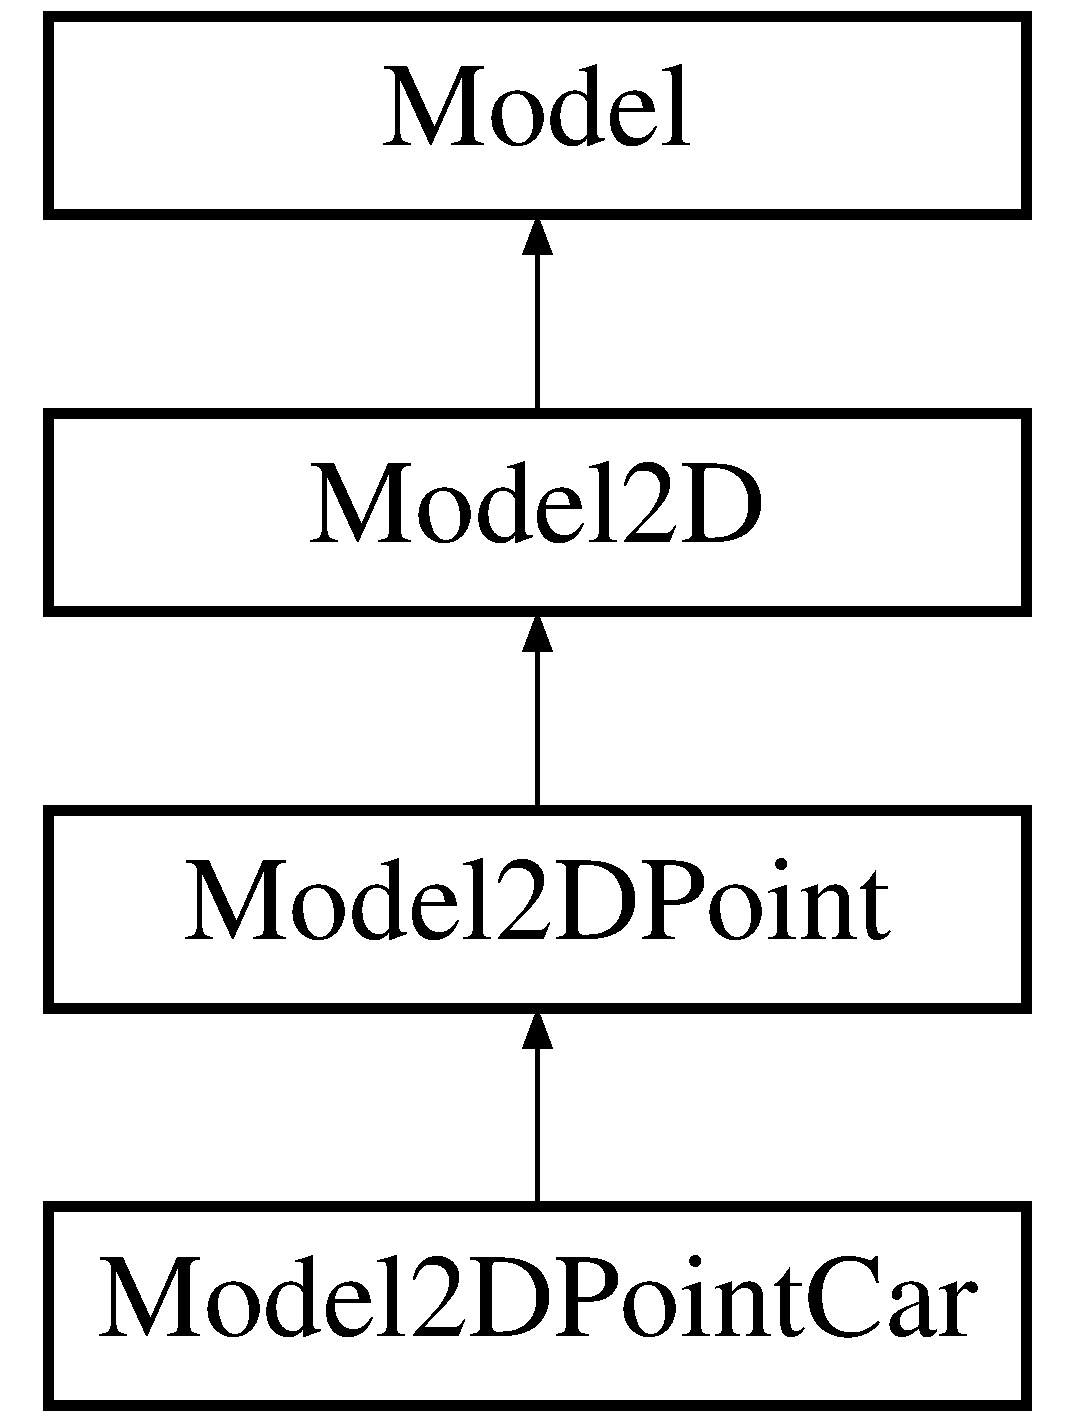
\includegraphics[height=4cm]{classModel2DPoint}
\end{center}
\end{figure}
\subsection*{Public Methods}
\begin{CompactItemize}
\item 
{\bf Model2DPoint} (string path)
\item 
virtual {\bf $\sim$Model2DPoint} ()
\item 
virtual {\bf MSLVector} {\bf Integrate} (const {\bf MSLVector} \&x, const {\bf MSLVector} \&u, const double \&h)
\begin{CompactList}\small\item\em Perform integration from state x, using input u, over time step h.\item\end{CompactList}\item 
virtual {\bf MSLVector} {\bf State\-Transition\-Equation} (const {\bf MSLVector} \&x, const {\bf MSLVector} \&u)
\begin{CompactList}\small\item\em The state transition equation, or equations of motion, xdot=f(x,u).\item\end{CompactList}\item 
virtual double {\bf Metric} (const {\bf MSLVector} \&x1, const {\bf MSLVector} \&x2)
\begin{CompactList}\small\item\em A distance metric, which is Euclidean in the base class.\item\end{CompactList}\end{CompactItemize}


\subsection{Detailed Description}
A point robot in a 2D world.



\subsection{Constructor \& Destructor Documentation}
\index{Model2DPoint@{Model2DPoint}!Model2DPoint@{Model2DPoint}}
\index{Model2DPoint@{Model2DPoint}!Model2DPoint@{Model2DPoint}}
\subsubsection{\setlength{\rightskip}{0pt plus 5cm}Model2DPoint::Model2DPoint (string {\em path} = \char`\"{}\char`\"{})}\label{classModel2DPoint_a0}


\index{Model2DPoint@{Model2DPoint}!~Model2DPoint@{$\sim$Model2DPoint}}
\index{~Model2DPoint@{$\sim$Model2DPoint}!Model2DPoint@{Model2DPoint}}
\subsubsection{\setlength{\rightskip}{0pt plus 5cm}Model2DPoint::$\sim$Model2DPoint ()\hspace{0.3cm}{\tt  [inline, virtual]}}\label{classModel2DPoint_a1}




\subsection{Member Function Documentation}
\index{Model2DPoint@{Model2DPoint}!Integrate@{Integrate}}
\index{Integrate@{Integrate}!Model2DPoint@{Model2DPoint}}
\subsubsection{\setlength{\rightskip}{0pt plus 5cm}{\bf MSLVector} Model2DPoint::Integrate (const {\bf MSLVector} \& {\em x}, const {\bf MSLVector} \& {\em u}, const double \& {\em h})\hspace{0.3cm}{\tt  [virtual]}}\label{classModel2DPoint_a2}


Perform integration from state x, using input u, over time step h.



Reimplemented from {\bf Model} {\rm (p.\,\pageref{classModel_a5})}.

Reimplemented in {\bf Model2DPoint\-Car} {\rm (p.\,\pageref{classModel2DPointCar_a2})}.\index{Model2DPoint@{Model2DPoint}!Metric@{Metric}}
\index{Metric@{Metric}!Model2DPoint@{Model2DPoint}}
\subsubsection{\setlength{\rightskip}{0pt plus 5cm}double Model2DPoint::Metric (const {\bf MSLVector} \& {\em x1}, const {\bf MSLVector} \& {\em x2})\hspace{0.3cm}{\tt  [virtual]}}\label{classModel2DPoint_a4}


A distance metric, which is Euclidean in the base class.



Reimplemented from {\bf Model} {\rm (p.\,\pageref{classModel_a9})}.

Reimplemented in {\bf Model2DPoint\-Car} {\rm (p.\,\pageref{classModel2DPointCar_a4})}.\index{Model2DPoint@{Model2DPoint}!StateTransitionEquation@{StateTransitionEquation}}
\index{StateTransitionEquation@{StateTransitionEquation}!Model2DPoint@{Model2DPoint}}
\subsubsection{\setlength{\rightskip}{0pt plus 5cm}{\bf MSLVector} Model2DPoint::State\-Transition\-Equation (const {\bf MSLVector} \& {\em x}, const {\bf MSLVector} \& {\em u})\hspace{0.3cm}{\tt  [virtual]}}\label{classModel2DPoint_a3}


The state transition equation, or equations of motion, xdot=f(x,u).



Reimplemented from {\bf Model} {\rm (p.\,\pageref{classModel_a3})}.

Reimplemented in {\bf Model2DPoint\-Car} {\rm (p.\,\pageref{classModel2DPointCar_a3})}.

The documentation for this class was generated from the following files:\begin{CompactItemize}
\item 
{\bf model2d.h}\item 
{\bf model2d.C}\end{CompactItemize}

\section{Model2DPoint\-Car  Class Reference}
\label{classModel2DPointCar}\index{Model2DPointCar@{Model2DPoint\-Car}}
A point car-like robot in a 2D world. 


{\tt \#include $<$model2d.h$>$}

Inheritance diagram for Model2DPoint\-Car::\begin{figure}[H]
\begin{center}
\leavevmode
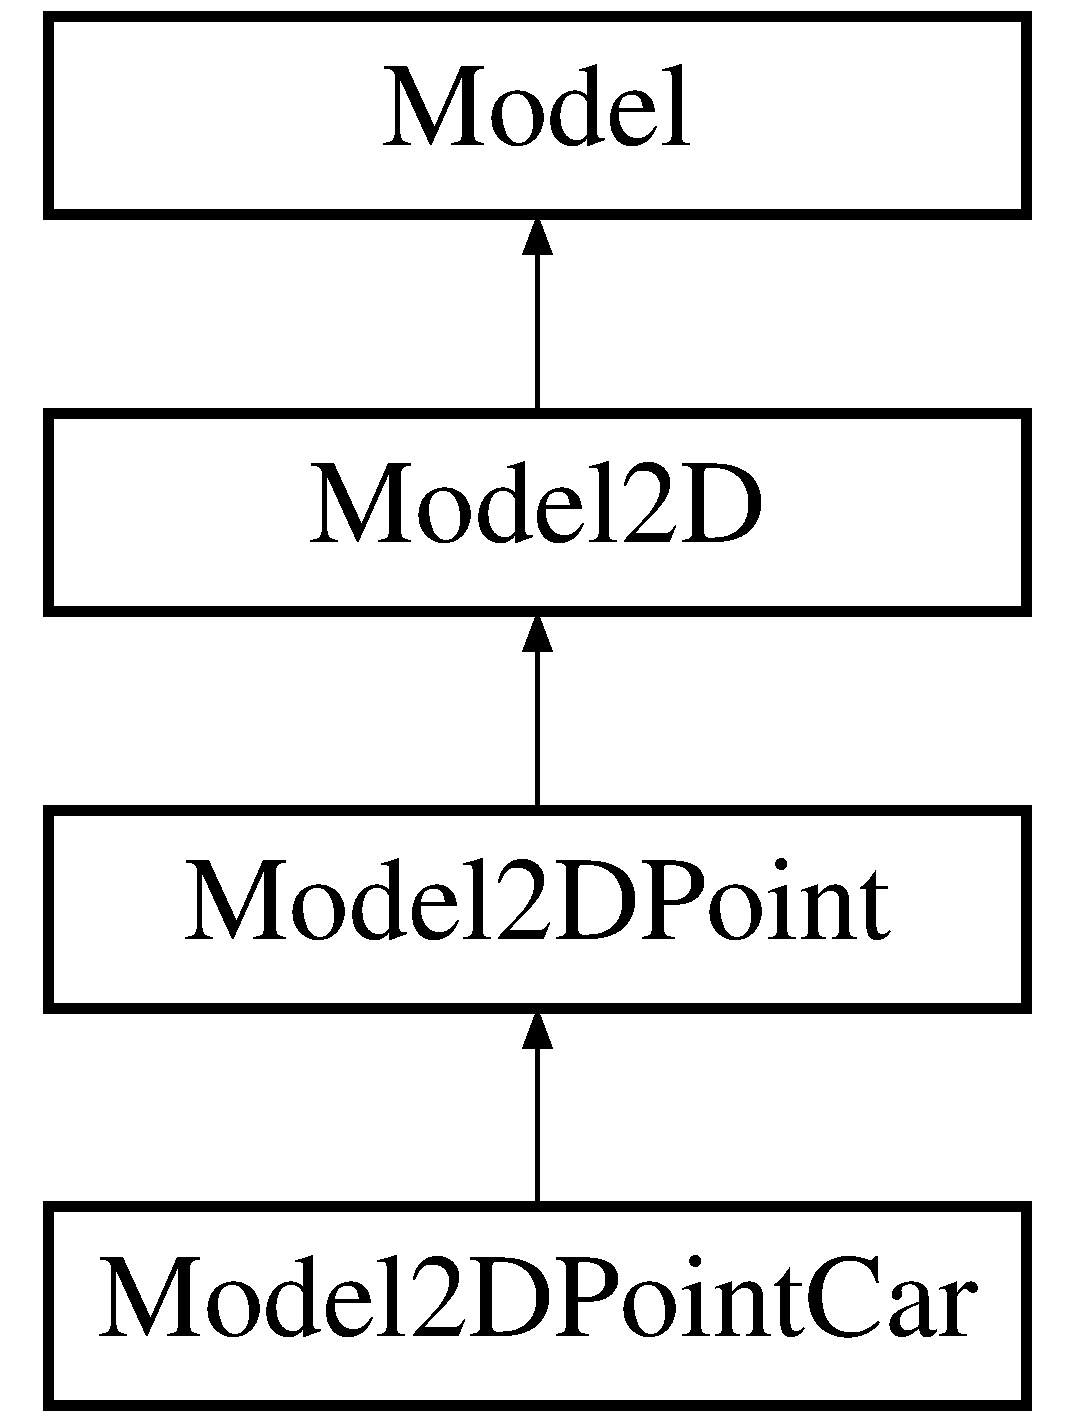
\includegraphics[height=4cm]{classModel2DPointCar}
\end{center}
\end{figure}
\subsection*{Public Methods}
\begin{CompactItemize}
\item 
{\bf Model2DPoint\-Car} (string path)
\item 
virtual {\bf $\sim$Model2DPoint\-Car} ()
\item 
virtual {\bf MSLVector} {\bf Integrate} (const {\bf MSLVector} \&x, const {\bf MSLVector} \&u, const double \&h)
\begin{CompactList}\small\item\em Perform integration from state x, using input u, over time step h.\item\end{CompactList}\item 
virtual {\bf MSLVector} {\bf State\-Transition\-Equation} (const {\bf MSLVector} \&x, const {\bf MSLVector} \&u)
\begin{CompactList}\small\item\em The state transition equation, or equations of motion, xdot=f(x,u).\item\end{CompactList}\item 
virtual double {\bf Metric} (const {\bf MSLVector} \&x1, const {\bf MSLVector} \&x2)
\begin{CompactList}\small\item\em A distance metric, which is Euclidean in the base class.\item\end{CompactList}\end{CompactItemize}
\subsection*{Public Attributes}
\begin{CompactItemize}
\item 
double {\bf Max\-Steering\-Angle}
\item 
double {\bf Car\-Length}
\end{CompactItemize}


\subsection{Detailed Description}
A point car-like robot in a 2D world.



\subsection{Constructor \& Destructor Documentation}
\index{Model2DPointCar@{Model2DPoint\-Car}!Model2DPointCar@{Model2DPointCar}}
\index{Model2DPointCar@{Model2DPointCar}!Model2DPointCar@{Model2DPoint\-Car}}
\subsubsection{\setlength{\rightskip}{0pt plus 5cm}Model2DPoint\-Car::Model2DPoint\-Car (string {\em path} = \char`\"{}\char`\"{})}\label{classModel2DPointCar_a0}


\index{Model2DPointCar@{Model2DPoint\-Car}!~Model2DPointCar@{$\sim$Model2DPointCar}}
\index{~Model2DPointCar@{$\sim$Model2DPointCar}!Model2DPointCar@{Model2DPoint\-Car}}
\subsubsection{\setlength{\rightskip}{0pt plus 5cm}Model2DPoint\-Car::$\sim$Model2DPoint\-Car ()\hspace{0.3cm}{\tt  [inline, virtual]}}\label{classModel2DPointCar_a1}




\subsection{Member Function Documentation}
\index{Model2DPointCar@{Model2DPoint\-Car}!Integrate@{Integrate}}
\index{Integrate@{Integrate}!Model2DPointCar@{Model2DPoint\-Car}}
\subsubsection{\setlength{\rightskip}{0pt plus 5cm}{\bf MSLVector} Model2DPoint\-Car::Integrate (const {\bf MSLVector} \& {\em x}, const {\bf MSLVector} \& {\em u}, const double \& {\em h})\hspace{0.3cm}{\tt  [virtual]}}\label{classModel2DPointCar_a2}


Perform integration from state x, using input u, over time step h.



Reimplemented from {\bf Model2DPoint} {\rm (p.\,\pageref{classModel2DPoint_a2})}.\index{Model2DPointCar@{Model2DPoint\-Car}!Metric@{Metric}}
\index{Metric@{Metric}!Model2DPointCar@{Model2DPoint\-Car}}
\subsubsection{\setlength{\rightskip}{0pt plus 5cm}double Model2DPoint\-Car::Metric (const {\bf MSLVector} \& {\em x1}, const {\bf MSLVector} \& {\em x2})\hspace{0.3cm}{\tt  [virtual]}}\label{classModel2DPointCar_a4}


A distance metric, which is Euclidean in the base class.



Reimplemented from {\bf Model2DPoint} {\rm (p.\,\pageref{classModel2DPoint_a4})}.\index{Model2DPointCar@{Model2DPoint\-Car}!StateTransitionEquation@{StateTransitionEquation}}
\index{StateTransitionEquation@{StateTransitionEquation}!Model2DPointCar@{Model2DPoint\-Car}}
\subsubsection{\setlength{\rightskip}{0pt plus 5cm}{\bf MSLVector} Model2DPoint\-Car::State\-Transition\-Equation (const {\bf MSLVector} \& {\em x}, const {\bf MSLVector} \& {\em u})\hspace{0.3cm}{\tt  [virtual]}}\label{classModel2DPointCar_a3}


The state transition equation, or equations of motion, xdot=f(x,u).



Reimplemented from {\bf Model2DPoint} {\rm (p.\,\pageref{classModel2DPoint_a3})}.

\subsection{Member Data Documentation}
\index{Model2DPointCar@{Model2DPoint\-Car}!CarLength@{CarLength}}
\index{CarLength@{CarLength}!Model2DPointCar@{Model2DPoint\-Car}}
\subsubsection{\setlength{\rightskip}{0pt plus 5cm}double Model2DPoint\-Car::Car\-Length}\label{classModel2DPointCar_m1}


\index{Model2DPointCar@{Model2DPoint\-Car}!MaxSteeringAngle@{MaxSteeringAngle}}
\index{MaxSteeringAngle@{MaxSteeringAngle}!Model2DPointCar@{Model2DPoint\-Car}}
\subsubsection{\setlength{\rightskip}{0pt plus 5cm}double Model2DPoint\-Car::Max\-Steering\-Angle}\label{classModel2DPointCar_m0}




The documentation for this class was generated from the following files:\begin{CompactItemize}
\item 
{\bf model2d.h}\item 
{\bf model2d.C}\end{CompactItemize}

\section{Model2DRigid  Class Reference}
\label{classModel2DRigid}\index{Model2DRigid@{Model2DRigid}}
A holonomic rigid robot in a 2D world. 


{\tt \#include $<$model2d.h$>$}

Inheritance diagram for Model2DRigid::\begin{figure}[H]
\begin{center}
\leavevmode
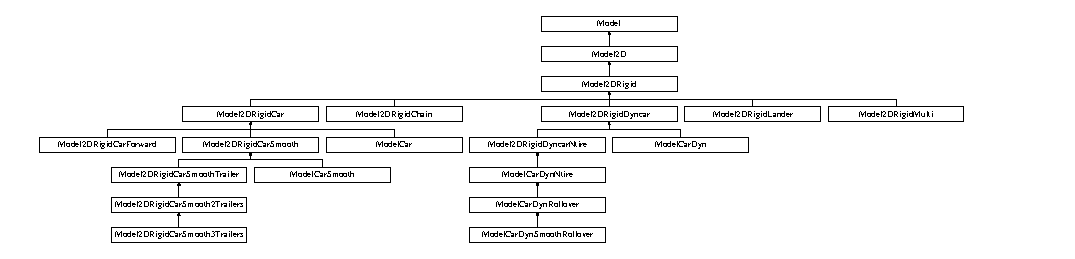
\includegraphics[height=3.03318cm]{classModel2DRigid}
\end{center}
\end{figure}
\subsection*{Public Methods}
\begin{CompactItemize}
\item 
{\bf Model2DRigid} (string path)
\item 
virtual {\bf $\sim$Model2DRigid} ()
\item 
virtual {\bf MSLVector} {\bf Integrate} (const {\bf MSLVector} \&x, const {\bf MSLVector} \&u, const double \&h)
\begin{CompactList}\small\item\em Perform integration from state x, using input u, over time step h.\item\end{CompactList}\item 
virtual {\bf MSLVector} {\bf State\-Transition\-Equation} (const {\bf MSLVector} \&x, const {\bf MSLVector} \&u)
\begin{CompactList}\small\item\em The state transition equation, or equations of motion, xdot=f(x,u).\item\end{CompactList}\item 
{\bf MSLVector} {\bf Linear\-Interpolate} (const {\bf MSLVector} \&x1, const {\bf MSLVector} \&x2, const double \&a)
\begin{CompactList}\small\item\em Linearly interpolate two state while respecting topology.\item\end{CompactList}\item 
virtual double {\bf Metric} (const {\bf MSLVector} \&x1, const {\bf MSLVector} \&x2)
\begin{CompactList}\small\item\em A distance metric, which is Euclidean in the base class.\item\end{CompactList}\item 
virtual {\bf MSLVector} {\bf State\-To\-Configuration} (const {\bf MSLVector} \&x)
\begin{CompactList}\small\item\em A method that converts a {\bf Model} {\rm (p.\,\pageref{classModel})} state in to a {\bf Geom} {\rm (p.\,\pageref{classGeom})} configuration.\item\end{CompactList}\end{CompactItemize}


\subsection{Detailed Description}
A holonomic rigid robot in a 2D world.



\subsection{Constructor \& Destructor Documentation}
\index{Model2DRigid@{Model2DRigid}!Model2DRigid@{Model2DRigid}}
\index{Model2DRigid@{Model2DRigid}!Model2DRigid@{Model2DRigid}}
\subsubsection{\setlength{\rightskip}{0pt plus 5cm}Model2DRigid::Model2DRigid (string {\em path} = \char`\"{}\char`\"{})}\label{classModel2DRigid_a0}


\index{Model2DRigid@{Model2DRigid}!~Model2DRigid@{$\sim$Model2DRigid}}
\index{~Model2DRigid@{$\sim$Model2DRigid}!Model2DRigid@{Model2DRigid}}
\subsubsection{\setlength{\rightskip}{0pt plus 5cm}Model2DRigid::$\sim$Model2DRigid ()\hspace{0.3cm}{\tt  [inline, virtual]}}\label{classModel2DRigid_a1}




\subsection{Member Function Documentation}
\index{Model2DRigid@{Model2DRigid}!Integrate@{Integrate}}
\index{Integrate@{Integrate}!Model2DRigid@{Model2DRigid}}
\subsubsection{\setlength{\rightskip}{0pt plus 5cm}{\bf MSLVector} Model2DRigid::Integrate (const {\bf MSLVector} \& {\em x}, const {\bf MSLVector} \& {\em u}, const double \& {\em h})\hspace{0.3cm}{\tt  [virtual]}}\label{classModel2DRigid_a2}


Perform integration from state x, using input u, over time step h.



Reimplemented from {\bf Model} {\rm (p.\,\pageref{classModel_a5})}.

Reimplemented in {\bf Model2DRigid\-Car\-Smooth} {\rm (p.\,\pageref{classModel2DRigidCarSmooth_a3})}, {\bf Model2DRigid\-Dyncar} {\rm (p.\,\pageref{classModel2DRigidDyncar_a2})}, {\bf Model2DRigid\-Lander} {\rm (p.\,\pageref{classModel2DRigidLander_a2})}, and {\bf Model\-Car\-Dyn\-Rollover} {\rm (p.\,\pageref{classModelCarDynRollover_a5})}.\index{Model2DRigid@{Model2DRigid}!LinearInterpolate@{LinearInterpolate}}
\index{LinearInterpolate@{LinearInterpolate}!Model2DRigid@{Model2DRigid}}
\subsubsection{\setlength{\rightskip}{0pt plus 5cm}{\bf MSLVector} Model2DRigid::Linear\-Interpolate (const {\bf MSLVector} \& {\em x1}, const {\bf MSLVector} \& {\em x2}, const double \& {\em a})\hspace{0.3cm}{\tt  [virtual]}}\label{classModel2DRigid_a4}


Linearly interpolate two state while respecting topology.

If a=0, then x1 is returned; if a=1, then x2 is returned. All intermediate values of \$a $\backslash$in [0,1]\$ yield intermediate states. This method is defined by {\bf Model} {\rm (p.\,\pageref{classModel})}. 

Reimplemented from {\bf Model} {\rm (p.\,\pageref{classModel_a6})}.

Reimplemented in {\bf Model2DRigid\-Dyncar} {\rm (p.\,\pageref{classModel2DRigidDyncar_a6})}, {\bf Model2DRigid\-Multi} {\rm (p.\,\pageref{classModel2DRigidMulti_a4})}, {\bf Model2DRigid\-Chain} {\rm (p.\,\pageref{classModel2DRigidChain_a4})}, and {\bf Model\-Car\-Dyn\-Smooth\-Rollover} {\rm (p.\,\pageref{classModelCarDynSmoothRollover_a5})}.\index{Model2DRigid@{Model2DRigid}!Metric@{Metric}}
\index{Metric@{Metric}!Model2DRigid@{Model2DRigid}}
\subsubsection{\setlength{\rightskip}{0pt plus 5cm}double Model2DRigid::Metric (const {\bf MSLVector} \& {\em x1}, const {\bf MSLVector} \& {\em x2})\hspace{0.3cm}{\tt  [virtual]}}\label{classModel2DRigid_a5}


A distance metric, which is Euclidean in the base class.



Reimplemented from {\bf Model} {\rm (p.\,\pageref{classModel_a9})}.

Reimplemented in {\bf Model2DRigid\-Car\-Smooth} {\rm (p.\,\pageref{classModel2DRigidCarSmooth_a4})}, {\bf Model2DRigid\-Car\-Smooth\-Trailer} {\rm (p.\,\pageref{classModel2DRigidCarSmoothTrailer_a3})}, {\bf Model2DRigid\-Car\-Smooth2Trailers} {\rm (p.\,\pageref{classModel2DRigidCarSmooth2Trailers_a3})}, {\bf Model2DRigid\-Car\-Smooth3Trailers} {\rm (p.\,\pageref{classModel2DRigidCarSmooth3Trailers_a3})}, {\bf Model2DRigid\-Dyncar} {\rm (p.\,\pageref{classModel2DRigidDyncar_a5})}, {\bf Model2DRigid\-Lander} {\rm (p.\,\pageref{classModel2DRigidLander_a5})}, {\bf Model2DRigid\-Multi} {\rm (p.\,\pageref{classModel2DRigidMulti_a2})}, {\bf Model2DRigid\-Chain} {\rm (p.\,\pageref{classModel2DRigidChain_a5})}, {\bf Model\-Car\-Dyn} {\rm (p.\,\pageref{classModelCarDyn_a3})}, {\bf Model\-Car\-Dyn\-Ntire} {\rm (p.\,\pageref{classModelCarDynNtire_a3})}, {\bf Model\-Car\-Dyn\-Rollover} {\rm (p.\,\pageref{classModelCarDynRollover_a6})}, and {\bf Model\-Car\-Dyn\-Smooth\-Rollover} {\rm (p.\,\pageref{classModelCarDynSmoothRollover_a4})}.\index{Model2DRigid@{Model2DRigid}!StateToConfiguration@{StateToConfiguration}}
\index{StateToConfiguration@{StateToConfiguration}!Model2DRigid@{Model2DRigid}}
\subsubsection{\setlength{\rightskip}{0pt plus 5cm}{\bf MSLVector} Model2DRigid::State\-To\-Configuration (const {\bf MSLVector} \& {\em x})\hspace{0.3cm}{\tt  [virtual]}}\label{classModel2DRigid_a6}


A method that converts a {\bf Model} {\rm (p.\,\pageref{classModel})} state in to a {\bf Geom} {\rm (p.\,\pageref{classGeom})} configuration.



Reimplemented from {\bf Model2D} {\rm (p.\,\pageref{classModel2D_a2})}.

Reimplemented in {\bf Model2DRigid\-Car\-Smooth} {\rm (p.\,\pageref{classModel2DRigidCarSmooth_a5})}, {\bf Model2DRigid\-Car\-Smooth\-Trailer} {\rm (p.\,\pageref{classModel2DRigidCarSmoothTrailer_a4})}, {\bf Model2DRigid\-Car\-Smooth2Trailers} {\rm (p.\,\pageref{classModel2DRigidCarSmooth2Trailers_a4})}, {\bf Model2DRigid\-Car\-Smooth3Trailers} {\rm (p.\,\pageref{classModel2DRigidCarSmooth3Trailers_a4})}, {\bf Model2DRigid\-Dyncar} {\rm (p.\,\pageref{classModel2DRigidDyncar_a3})}, {\bf Model2DRigid\-Lander} {\rm (p.\,\pageref{classModel2DRigidLander_a3})}, {\bf Model2DRigid\-Multi} {\rm (p.\,\pageref{classModel2DRigidMulti_a3})}, {\bf Model2DRigid\-Chain} {\rm (p.\,\pageref{classModel2DRigidChain_a2})}, {\bf Model\-Car} {\rm (p.\,\pageref{classModelCar_a2})}, {\bf Model\-Car\-Smooth} {\rm (p.\,\pageref{classModelCarSmooth_a2})}, {\bf Model\-Car\-Dyn} {\rm (p.\,\pageref{classModelCarDyn_a2})}, {\bf Model\-Car\-Dyn\-Ntire} {\rm (p.\,\pageref{classModelCarDynNtire_a2})}, {\bf Model\-Car\-Dyn\-Rollover} {\rm (p.\,\pageref{classModelCarDynRollover_a4})}, and {\bf Model\-Car\-Dyn\-Smooth\-Rollover} {\rm (p.\,\pageref{classModelCarDynSmoothRollover_a3})}.\index{Model2DRigid@{Model2DRigid}!StateTransitionEquation@{StateTransitionEquation}}
\index{StateTransitionEquation@{StateTransitionEquation}!Model2DRigid@{Model2DRigid}}
\subsubsection{\setlength{\rightskip}{0pt plus 5cm}{\bf MSLVector} Model2DRigid::State\-Transition\-Equation (const {\bf MSLVector} \& {\em x}, const {\bf MSLVector} \& {\em u})\hspace{0.3cm}{\tt  [virtual]}}\label{classModel2DRigid_a3}


The state transition equation, or equations of motion, xdot=f(x,u).



Reimplemented from {\bf Model} {\rm (p.\,\pageref{classModel_a3})}.

Reimplemented in {\bf Model2DRigid\-Car} {\rm (p.\,\pageref{classModel2DRigidCar_a2})}, {\bf Model2DRigid\-Car\-Smooth} {\rm (p.\,\pageref{classModel2DRigidCarSmooth_a2})}, {\bf Model2DRigid\-Car\-Smooth\-Trailer} {\rm (p.\,\pageref{classModel2DRigidCarSmoothTrailer_a2})}, {\bf Model2DRigid\-Car\-Smooth2Trailers} {\rm (p.\,\pageref{classModel2DRigidCarSmooth2Trailers_a2})}, {\bf Model2DRigid\-Car\-Smooth3Trailers} {\rm (p.\,\pageref{classModel2DRigidCarSmooth3Trailers_a2})}, {\bf Model2DRigid\-Dyncar} {\rm (p.\,\pageref{classModel2DRigidDyncar_a4})}, {\bf Model2DRigid\-Dyncar\-Ntire} {\rm (p.\,\pageref{classModel2DRigidDyncarNtire_a2})}, {\bf Model2DRigid\-Lander} {\rm (p.\,\pageref{classModel2DRigidLander_a4})}, {\bf Model2DRigid\-Chain} {\rm (p.\,\pageref{classModel2DRigidChain_a3})}, {\bf Model\-Car\-Dyn\-Rollover} {\rm (p.\,\pageref{classModelCarDynRollover_a3})}, and {\bf Model\-Car\-Dyn\-Smooth\-Rollover} {\rm (p.\,\pageref{classModelCarDynSmoothRollover_a2})}.

The documentation for this class was generated from the following files:\begin{CompactItemize}
\item 
{\bf model2d.h}\item 
{\bf model2d.C}\end{CompactItemize}

\section{Model2DRigid\-Car  Class Reference}
\label{classModel2DRigidCar}\index{Model2DRigidCar@{Model2DRigid\-Car}}
A rigid car-like robot in a 2D world. 


{\tt \#include $<$model2d.h$>$}

Inheritance diagram for Model2DRigid\-Car::\begin{figure}[H]
\begin{center}
\leavevmode
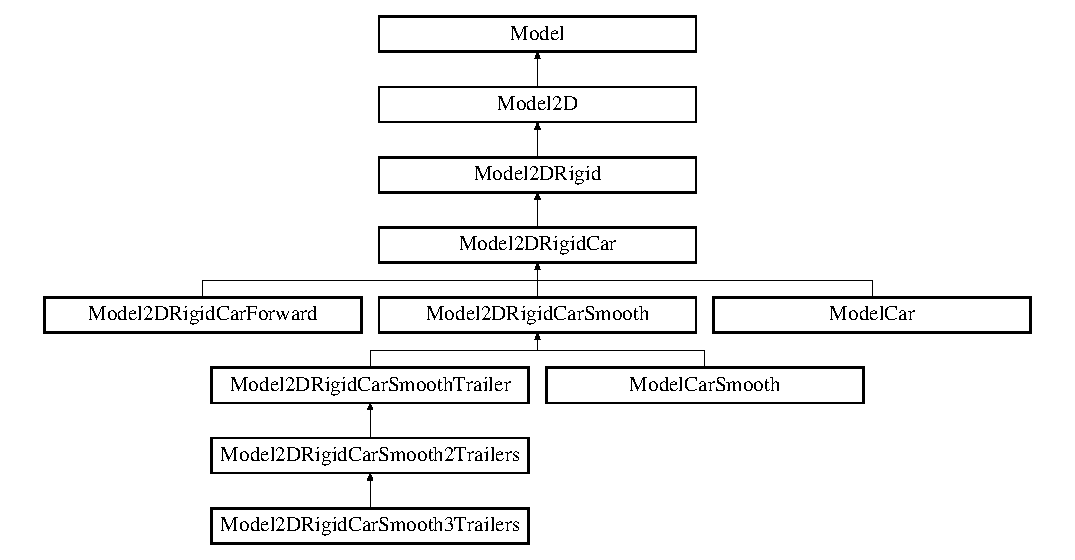
\includegraphics[height=7.07741cm]{classModel2DRigidCar}
\end{center}
\end{figure}
\subsection*{Public Methods}
\begin{CompactItemize}
\item 
{\bf Model2DRigid\-Car} (string path)
\item 
virtual {\bf $\sim$Model2DRigid\-Car} ()
\item 
virtual {\bf MSLVector} {\bf State\-Transition\-Equation} (const {\bf MSLVector} \&x, const {\bf MSLVector} \&u)
\begin{CompactList}\small\item\em The state transition equation, or equations of motion, xdot=f(x,u).\item\end{CompactList}\end{CompactItemize}
\subsection*{Public Attributes}
\begin{CompactItemize}
\item 
double {\bf Max\-Steering\-Angle}
\item 
double {\bf Car\-Length}
\end{CompactItemize}


\subsection{Detailed Description}
A rigid car-like robot in a 2D world.



\subsection{Constructor \& Destructor Documentation}
\index{Model2DRigidCar@{Model2DRigid\-Car}!Model2DRigidCar@{Model2DRigidCar}}
\index{Model2DRigidCar@{Model2DRigidCar}!Model2DRigidCar@{Model2DRigid\-Car}}
\subsubsection{\setlength{\rightskip}{0pt plus 5cm}Model2DRigid\-Car::Model2DRigid\-Car (string {\em path} = \char`\"{}\char`\"{})}\label{classModel2DRigidCar_a0}


\index{Model2DRigidCar@{Model2DRigid\-Car}!~Model2DRigidCar@{$\sim$Model2DRigidCar}}
\index{~Model2DRigidCar@{$\sim$Model2DRigidCar}!Model2DRigidCar@{Model2DRigid\-Car}}
\subsubsection{\setlength{\rightskip}{0pt plus 5cm}Model2DRigid\-Car::$\sim$Model2DRigid\-Car ()\hspace{0.3cm}{\tt  [inline, virtual]}}\label{classModel2DRigidCar_a1}




\subsection{Member Function Documentation}
\index{Model2DRigidCar@{Model2DRigid\-Car}!StateTransitionEquation@{StateTransitionEquation}}
\index{StateTransitionEquation@{StateTransitionEquation}!Model2DRigidCar@{Model2DRigid\-Car}}
\subsubsection{\setlength{\rightskip}{0pt plus 5cm}{\bf MSLVector} Model2DRigid\-Car::State\-Transition\-Equation (const {\bf MSLVector} \& {\em x}, const {\bf MSLVector} \& {\em u})\hspace{0.3cm}{\tt  [virtual]}}\label{classModel2DRigidCar_a2}


The state transition equation, or equations of motion, xdot=f(x,u).



Reimplemented from {\bf Model2DRigid} {\rm (p.\,\pageref{classModel2DRigid_a3})}.

Reimplemented in {\bf Model2DRigid\-Car\-Smooth} {\rm (p.\,\pageref{classModel2DRigidCarSmooth_a2})}, {\bf Model2DRigid\-Car\-Smooth\-Trailer} {\rm (p.\,\pageref{classModel2DRigidCarSmoothTrailer_a2})}, {\bf Model2DRigid\-Car\-Smooth2Trailers} {\rm (p.\,\pageref{classModel2DRigidCarSmooth2Trailers_a2})}, and {\bf Model2DRigid\-Car\-Smooth3Trailers} {\rm (p.\,\pageref{classModel2DRigidCarSmooth3Trailers_a2})}.

\subsection{Member Data Documentation}
\index{Model2DRigidCar@{Model2DRigid\-Car}!CarLength@{CarLength}}
\index{CarLength@{CarLength}!Model2DRigidCar@{Model2DRigid\-Car}}
\subsubsection{\setlength{\rightskip}{0pt plus 5cm}double Model2DRigid\-Car::Car\-Length}\label{classModel2DRigidCar_m1}


\index{Model2DRigidCar@{Model2DRigid\-Car}!MaxSteeringAngle@{MaxSteeringAngle}}
\index{MaxSteeringAngle@{MaxSteeringAngle}!Model2DRigidCar@{Model2DRigid\-Car}}
\subsubsection{\setlength{\rightskip}{0pt plus 5cm}double Model2DRigid\-Car::Max\-Steering\-Angle}\label{classModel2DRigidCar_m0}




The documentation for this class was generated from the following files:\begin{CompactItemize}
\item 
{\bf model2d.h}\item 
{\bf model2d.C}\end{CompactItemize}

\section{Model2DRigid\-Car\-Forward  Class Reference}
\label{classModel2DRigidCarForward}\index{Model2DRigidCarForward@{Model2DRigid\-Car\-Forward}}
A rigid car-like robot that can only go forward in a 2D world. 


{\tt \#include $<$model2d.h$>$}

Inheritance diagram for Model2DRigid\-Car\-Forward::\begin{figure}[H]
\begin{center}
\leavevmode
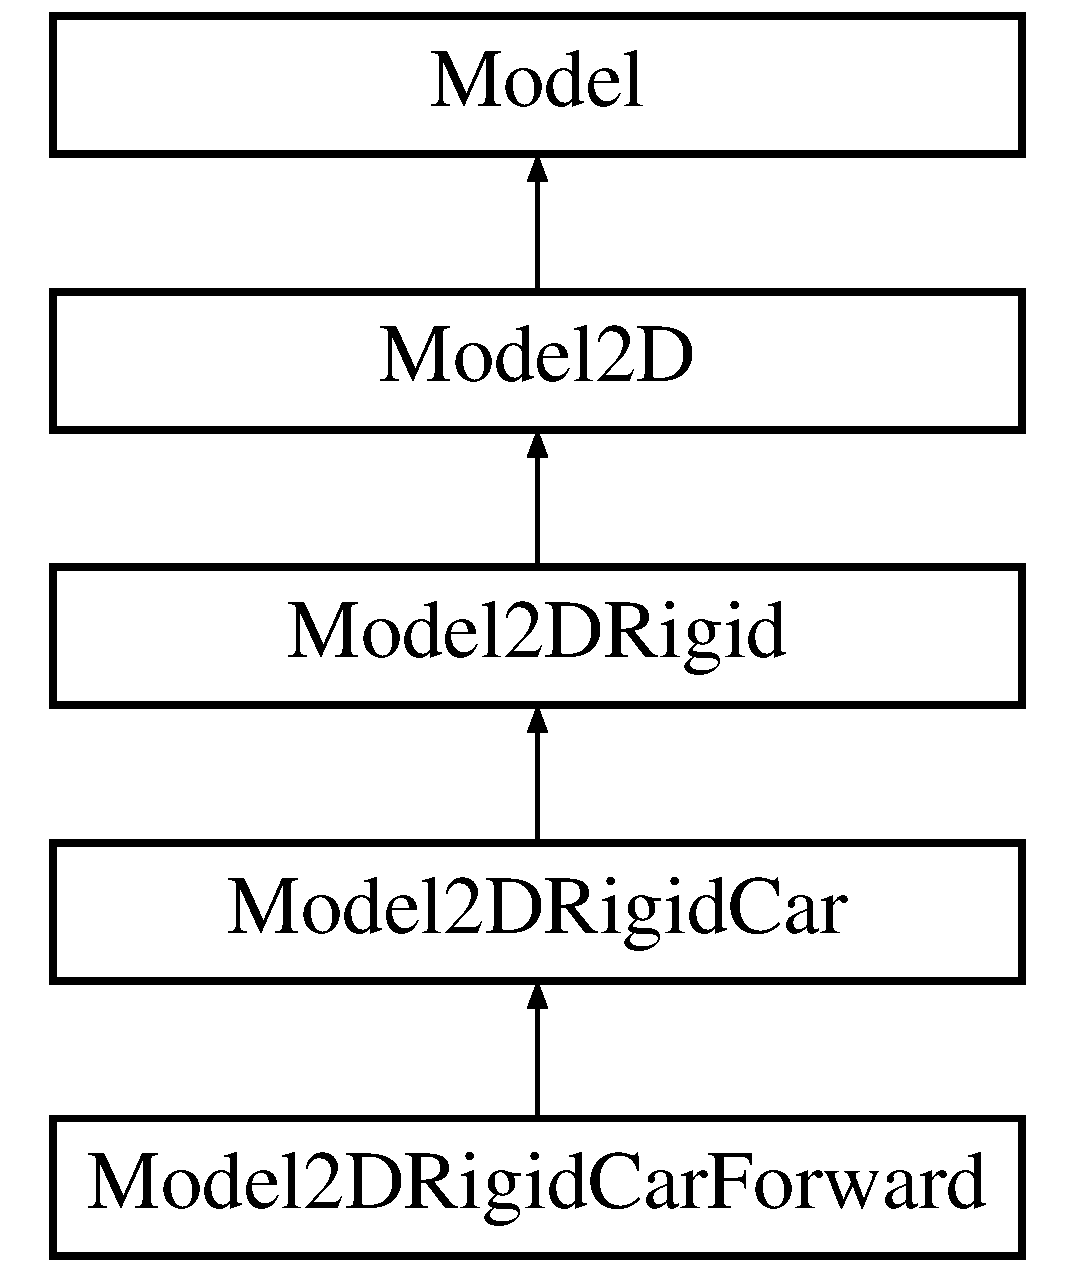
\includegraphics[height=5cm]{classModel2DRigidCarForward}
\end{center}
\end{figure}
\subsection*{Public Methods}
\begin{CompactItemize}
\item 
{\bf Model2DRigid\-Car\-Forward} (string path)
\item 
virtual {\bf $\sim$Model2DRigid\-Car\-Forward} ()
\end{CompactItemize}


\subsection{Detailed Description}
A rigid car-like robot that can only go forward in a 2D world.



\subsection{Constructor \& Destructor Documentation}
\index{Model2DRigidCarForward@{Model2DRigid\-Car\-Forward}!Model2DRigidCarForward@{Model2DRigidCarForward}}
\index{Model2DRigidCarForward@{Model2DRigidCarForward}!Model2DRigidCarForward@{Model2DRigid\-Car\-Forward}}
\subsubsection{\setlength{\rightskip}{0pt plus 5cm}Model2DRigid\-Car\-Forward::Model2DRigid\-Car\-Forward (string {\em path} = \char`\"{}\char`\"{})}\label{classModel2DRigidCarForward_a0}


\index{Model2DRigidCarForward@{Model2DRigid\-Car\-Forward}!~Model2DRigidCarForward@{$\sim$Model2DRigidCarForward}}
\index{~Model2DRigidCarForward@{$\sim$Model2DRigidCarForward}!Model2DRigidCarForward@{Model2DRigid\-Car\-Forward}}
\subsubsection{\setlength{\rightskip}{0pt plus 5cm}Model2DRigid\-Car\-Forward::$\sim$Model2DRigid\-Car\-Forward ()\hspace{0.3cm}{\tt  [inline, virtual]}}\label{classModel2DRigidCarForward_a1}




The documentation for this class was generated from the following files:\begin{CompactItemize}
\item 
{\bf model2d.h}\item 
{\bf model2d.C}\end{CompactItemize}

\section{Model2DRigid\-Car\-Smooth  Class Reference}
\label{classModel2DRigidCarSmooth}\index{Model2DRigidCarSmooth@{Model2DRigid\-Car\-Smooth}}
A rigid car-like robot with continuous steering angles This model is used by Th. Fraichard, Scheuer, Laugier. 


{\tt \#include $<$model2d.h$>$}

Inheritance diagram for Model2DRigid\-Car\-Smooth::\begin{figure}[H]
\begin{center}
\leavevmode
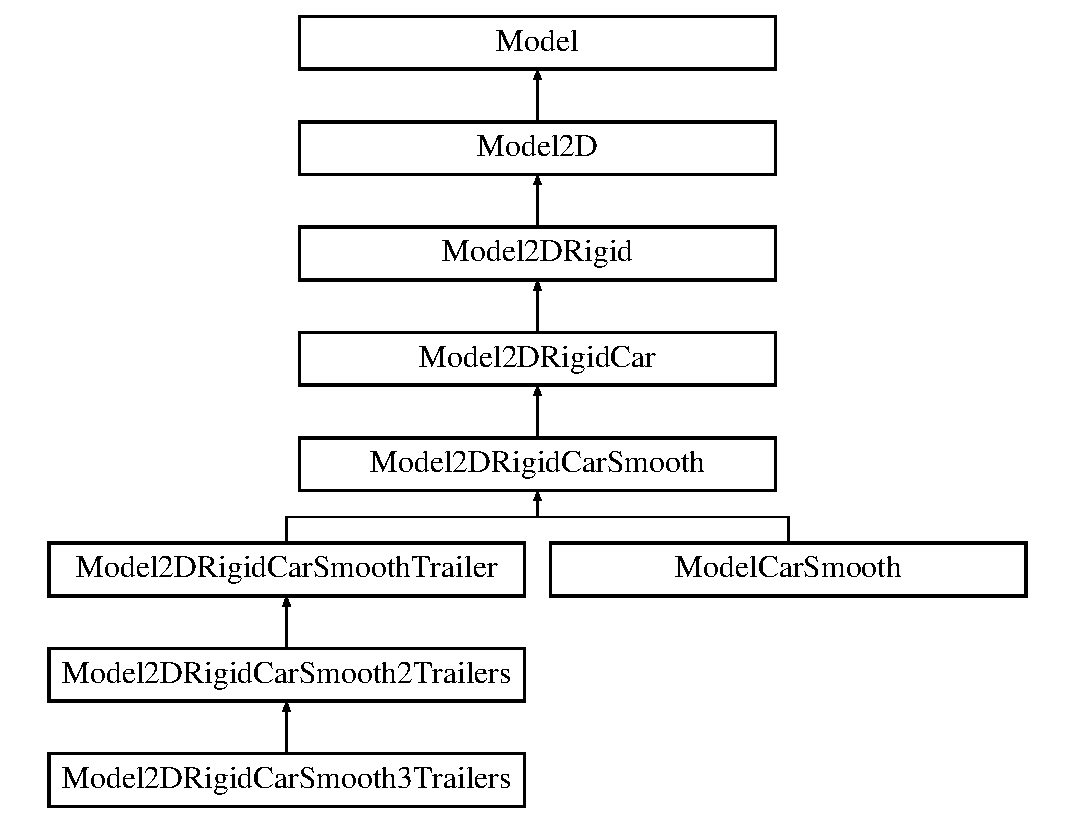
\includegraphics[height=8cm]{classModel2DRigidCarSmooth}
\end{center}
\end{figure}
\subsection*{Public Methods}
\begin{CompactItemize}
\item 
{\bf Model2DRigid\-Car\-Smooth} (string path)
\item 
virtual {\bf $\sim$Model2DRigid\-Car\-Smooth} ()
\item 
virtual {\bf MSLVector} {\bf State\-Transition\-Equation} (const {\bf MSLVector} \&x, const {\bf MSLVector} \&u)
\begin{CompactList}\small\item\em The state transition equation, or equations of motion, xdot=f(x,u).\item\end{CompactList}\item 
{\bf MSLVector} {\bf Integrate} (const {\bf MSLVector} \&x, const {\bf MSLVector} \&u, const double \&h)
\begin{CompactList}\small\item\em Perform integration from state x, using input u, over time step h.\item\end{CompactList}\item 
virtual double {\bf Metric} (const {\bf MSLVector} \&x1, const {\bf MSLVector} \&x2)
\begin{CompactList}\small\item\em A distance metric, which is Euclidean in the base class.\item\end{CompactList}\item 
virtual {\bf MSLVector} {\bf State\-To\-Configuration} (const {\bf MSLVector} \&x)
\begin{CompactList}\small\item\em A method that converts a {\bf Model} {\rm (p.\,\pageref{classModel})} state in to a {\bf Geom} {\rm (p.\,\pageref{classGeom})} configuration.\item\end{CompactList}\item 
virtual bool {\bf Satisfied} (const {\bf MSLVector} \&x)
\begin{CompactList}\small\item\em Test whether global state-space constraints are satisfied.\item\end{CompactList}\end{CompactItemize}
\subsection*{Public Attributes}
\begin{CompactItemize}
\item 
double {\bf Steering\-Speed}
\end{CompactItemize}


\subsection{Detailed Description}
A rigid car-like robot with continuous steering angles This model is used by Th. Fraichard, Scheuer, Laugier.



\subsection{Constructor \& Destructor Documentation}
\index{Model2DRigidCarSmooth@{Model2DRigid\-Car\-Smooth}!Model2DRigidCarSmooth@{Model2DRigidCarSmooth}}
\index{Model2DRigidCarSmooth@{Model2DRigidCarSmooth}!Model2DRigidCarSmooth@{Model2DRigid\-Car\-Smooth}}
\subsubsection{\setlength{\rightskip}{0pt plus 5cm}Model2DRigid\-Car\-Smooth::Model2DRigid\-Car\-Smooth (string {\em path} = \char`\"{}\char`\"{})}\label{classModel2DRigidCarSmooth_a0}


\index{Model2DRigidCarSmooth@{Model2DRigid\-Car\-Smooth}!~Model2DRigidCarSmooth@{$\sim$Model2DRigidCarSmooth}}
\index{~Model2DRigidCarSmooth@{$\sim$Model2DRigidCarSmooth}!Model2DRigidCarSmooth@{Model2DRigid\-Car\-Smooth}}
\subsubsection{\setlength{\rightskip}{0pt plus 5cm}Model2DRigid\-Car\-Smooth::$\sim$Model2DRigid\-Car\-Smooth ()\hspace{0.3cm}{\tt  [inline, virtual]}}\label{classModel2DRigidCarSmooth_a1}




\subsection{Member Function Documentation}
\index{Model2DRigidCarSmooth@{Model2DRigid\-Car\-Smooth}!Integrate@{Integrate}}
\index{Integrate@{Integrate}!Model2DRigidCarSmooth@{Model2DRigid\-Car\-Smooth}}
\subsubsection{\setlength{\rightskip}{0pt plus 5cm}{\bf MSLVector} Model2DRigid\-Car\-Smooth::Integrate (const {\bf MSLVector} \& {\em x}, const {\bf MSLVector} \& {\em u}, const double \& {\em h})\hspace{0.3cm}{\tt  [virtual]}}\label{classModel2DRigidCarSmooth_a3}


Perform integration from state x, using input u, over time step h.



Reimplemented from {\bf Model2DRigid} {\rm (p.\,\pageref{classModel2DRigid_a2})}.\index{Model2DRigidCarSmooth@{Model2DRigid\-Car\-Smooth}!Metric@{Metric}}
\index{Metric@{Metric}!Model2DRigidCarSmooth@{Model2DRigid\-Car\-Smooth}}
\subsubsection{\setlength{\rightskip}{0pt plus 5cm}double Model2DRigid\-Car\-Smooth::Metric (const {\bf MSLVector} \& {\em x1}, const {\bf MSLVector} \& {\em x2})\hspace{0.3cm}{\tt  [virtual]}}\label{classModel2DRigidCarSmooth_a4}


A distance metric, which is Euclidean in the base class.



Reimplemented from {\bf Model2DRigid} {\rm (p.\,\pageref{classModel2DRigid_a5})}.

Reimplemented in {\bf Model2DRigid\-Car\-Smooth\-Trailer} {\rm (p.\,\pageref{classModel2DRigidCarSmoothTrailer_a3})}, {\bf Model2DRigid\-Car\-Smooth2Trailers} {\rm (p.\,\pageref{classModel2DRigidCarSmooth2Trailers_a3})}, and {\bf Model2DRigid\-Car\-Smooth3Trailers} {\rm (p.\,\pageref{classModel2DRigidCarSmooth3Trailers_a3})}.\index{Model2DRigidCarSmooth@{Model2DRigid\-Car\-Smooth}!Satisfied@{Satisfied}}
\index{Satisfied@{Satisfied}!Model2DRigidCarSmooth@{Model2DRigid\-Car\-Smooth}}
\subsubsection{\setlength{\rightskip}{0pt plus 5cm}bool Model2DRigid\-Car\-Smooth::Satisfied (const {\bf MSLVector} \& {\em x})\hspace{0.3cm}{\tt  [virtual]}}\label{classModel2DRigidCarSmooth_a6}


Test whether global state-space constraints are satisfied.



Reimplemented from {\bf Model} {\rm (p.\,\pageref{classModel_a4})}.

Reimplemented in {\bf Model2DRigid\-Car\-Smooth\-Trailer} {\rm (p.\,\pageref{classModel2DRigidCarSmoothTrailer_a5})}, {\bf Model2DRigid\-Car\-Smooth2Trailers} {\rm (p.\,\pageref{classModel2DRigidCarSmooth2Trailers_a5})}, and {\bf Model2DRigid\-Car\-Smooth3Trailers} {\rm (p.\,\pageref{classModel2DRigidCarSmooth3Trailers_a5})}.\index{Model2DRigidCarSmooth@{Model2DRigid\-Car\-Smooth}!StateToConfiguration@{StateToConfiguration}}
\index{StateToConfiguration@{StateToConfiguration}!Model2DRigidCarSmooth@{Model2DRigid\-Car\-Smooth}}
\subsubsection{\setlength{\rightskip}{0pt plus 5cm}{\bf MSLVector} Model2DRigid\-Car\-Smooth::State\-To\-Configuration (const {\bf MSLVector} \& {\em x})\hspace{0.3cm}{\tt  [virtual]}}\label{classModel2DRigidCarSmooth_a5}


A method that converts a {\bf Model} {\rm (p.\,\pageref{classModel})} state in to a {\bf Geom} {\rm (p.\,\pageref{classGeom})} configuration.



Reimplemented from {\bf Model2DRigid} {\rm (p.\,\pageref{classModel2DRigid_a6})}.

Reimplemented in {\bf Model2DRigid\-Car\-Smooth\-Trailer} {\rm (p.\,\pageref{classModel2DRigidCarSmoothTrailer_a4})}, {\bf Model2DRigid\-Car\-Smooth2Trailers} {\rm (p.\,\pageref{classModel2DRigidCarSmooth2Trailers_a4})}, {\bf Model2DRigid\-Car\-Smooth3Trailers} {\rm (p.\,\pageref{classModel2DRigidCarSmooth3Trailers_a4})}, and {\bf Model\-Car\-Smooth} {\rm (p.\,\pageref{classModelCarSmooth_a2})}.\index{Model2DRigidCarSmooth@{Model2DRigid\-Car\-Smooth}!StateTransitionEquation@{StateTransitionEquation}}
\index{StateTransitionEquation@{StateTransitionEquation}!Model2DRigidCarSmooth@{Model2DRigid\-Car\-Smooth}}
\subsubsection{\setlength{\rightskip}{0pt plus 5cm}{\bf MSLVector} Model2DRigid\-Car\-Smooth::State\-Transition\-Equation (const {\bf MSLVector} \& {\em x}, const {\bf MSLVector} \& {\em u})\hspace{0.3cm}{\tt  [virtual]}}\label{classModel2DRigidCarSmooth_a2}


The state transition equation, or equations of motion, xdot=f(x,u).



Reimplemented from {\bf Model2DRigid\-Car} {\rm (p.\,\pageref{classModel2DRigidCar_a2})}.

Reimplemented in {\bf Model2DRigid\-Car\-Smooth\-Trailer} {\rm (p.\,\pageref{classModel2DRigidCarSmoothTrailer_a2})}, {\bf Model2DRigid\-Car\-Smooth2Trailers} {\rm (p.\,\pageref{classModel2DRigidCarSmooth2Trailers_a2})}, and {\bf Model2DRigid\-Car\-Smooth3Trailers} {\rm (p.\,\pageref{classModel2DRigidCarSmooth3Trailers_a2})}.

\subsection{Member Data Documentation}
\index{Model2DRigidCarSmooth@{Model2DRigid\-Car\-Smooth}!SteeringSpeed@{SteeringSpeed}}
\index{SteeringSpeed@{SteeringSpeed}!Model2DRigidCarSmooth@{Model2DRigid\-Car\-Smooth}}
\subsubsection{\setlength{\rightskip}{0pt plus 5cm}double Model2DRigid\-Car\-Smooth::Steering\-Speed}\label{classModel2DRigidCarSmooth_m0}




The documentation for this class was generated from the following files:\begin{CompactItemize}
\item 
{\bf model2d.h}\item 
{\bf model2d.C}\end{CompactItemize}

\section{Model2DRigid\-Car\-Smooth2Trailers  Class Reference}
\label{classModel2DRigidCarSmooth2Trailers}\index{Model2DRigidCarSmooth2Trailers@{Model2DRigid\-Car\-Smooth2Trailers}}
A rigid car-like robot with continuous steering angles and two trailers. 


{\tt \#include $<$model2d.h$>$}

Inheritance diagram for Model2DRigid\-Car\-Smooth2Trailers::\begin{figure}[H]
\begin{center}
\leavevmode
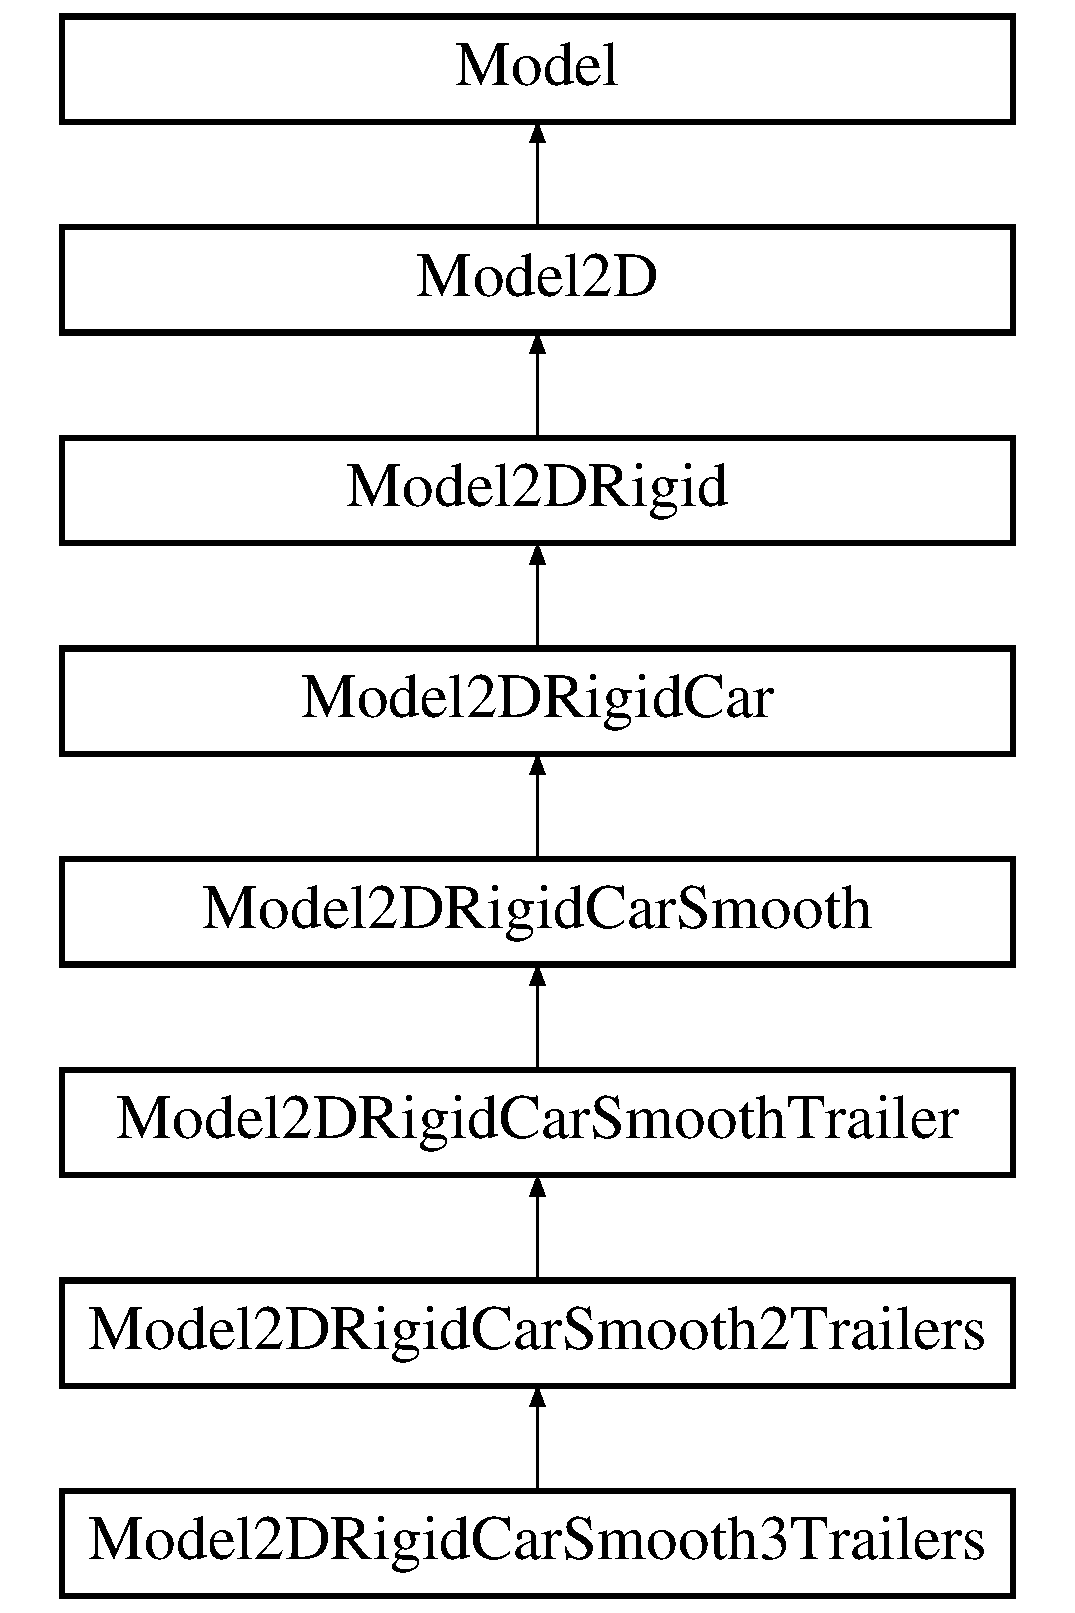
\includegraphics[height=8cm]{classModel2DRigidCarSmooth2Trailers}
\end{center}
\end{figure}
\subsection*{Public Methods}
\begin{CompactItemize}
\item 
{\bf Model2DRigid\-Car\-Smooth2Trailers} (string path)
\item 
virtual {\bf $\sim$Model2DRigid\-Car\-Smooth2Trailers} ()
\item 
virtual {\bf MSLVector} {\bf State\-Transition\-Equation} (const {\bf MSLVector} \&x, const {\bf MSLVector} \&u)
\begin{CompactList}\small\item\em The state transition equation, or equations of motion, xdot=f(x,u).\item\end{CompactList}\item 
virtual double {\bf Metric} (const {\bf MSLVector} \&x1, const {\bf MSLVector} \&x2)
\begin{CompactList}\small\item\em A distance metric, which is Euclidean in the base class.\item\end{CompactList}\item 
virtual {\bf MSLVector} {\bf State\-To\-Configuration} (const {\bf MSLVector} \&x)
\begin{CompactList}\small\item\em A method that converts a {\bf Model} {\rm (p.\,\pageref{classModel})} state in to a {\bf Geom} {\rm (p.\,\pageref{classGeom})} configuration.\item\end{CompactList}\item 
virtual bool {\bf Satisfied} (const {\bf MSLVector} \&x)
\begin{CompactList}\small\item\em Test whether global state-space constraints are satisfied.\item\end{CompactList}\end{CompactItemize}
\subsection*{Public Attributes}
\begin{CompactItemize}
\item 
double {\bf Hitch2Length}
\item 
double {\bf Hitch2Max\-Angle}
\end{CompactItemize}


\subsection{Detailed Description}
A rigid car-like robot with continuous steering angles and two trailers.



\subsection{Constructor \& Destructor Documentation}
\index{Model2DRigidCarSmooth2Trailers@{Model2DRigid\-Car\-Smooth2Trailers}!Model2DRigidCarSmooth2Trailers@{Model2DRigidCarSmooth2Trailers}}
\index{Model2DRigidCarSmooth2Trailers@{Model2DRigidCarSmooth2Trailers}!Model2DRigidCarSmooth2Trailers@{Model2DRigid\-Car\-Smooth2Trailers}}
\subsubsection{\setlength{\rightskip}{0pt plus 5cm}Model2DRigid\-Car\-Smooth2Trailers::Model2DRigid\-Car\-Smooth2Trailers (string {\em path} = \char`\"{}\char`\"{})}\label{classModel2DRigidCarSmooth2Trailers_a0}


\index{Model2DRigidCarSmooth2Trailers@{Model2DRigid\-Car\-Smooth2Trailers}!~Model2DRigidCarSmooth2Trailers@{$\sim$Model2DRigidCarSmooth2Trailers}}
\index{~Model2DRigidCarSmooth2Trailers@{$\sim$Model2DRigidCarSmooth2Trailers}!Model2DRigidCarSmooth2Trailers@{Model2DRigid\-Car\-Smooth2Trailers}}
\subsubsection{\setlength{\rightskip}{0pt plus 5cm}Model2DRigid\-Car\-Smooth2Trailers::$\sim$Model2DRigid\-Car\-Smooth2Trailers ()\hspace{0.3cm}{\tt  [inline, virtual]}}\label{classModel2DRigidCarSmooth2Trailers_a1}




\subsection{Member Function Documentation}
\index{Model2DRigidCarSmooth2Trailers@{Model2DRigid\-Car\-Smooth2Trailers}!Metric@{Metric}}
\index{Metric@{Metric}!Model2DRigidCarSmooth2Trailers@{Model2DRigid\-Car\-Smooth2Trailers}}
\subsubsection{\setlength{\rightskip}{0pt plus 5cm}double Model2DRigid\-Car\-Smooth2Trailers::Metric (const {\bf MSLVector} \& {\em x1}, const {\bf MSLVector} \& {\em x2})\hspace{0.3cm}{\tt  [virtual]}}\label{classModel2DRigidCarSmooth2Trailers_a3}


A distance metric, which is Euclidean in the base class.



Reimplemented from {\bf Model2DRigid\-Car\-Smooth\-Trailer} {\rm (p.\,\pageref{classModel2DRigidCarSmoothTrailer_a3})}.

Reimplemented in {\bf Model2DRigid\-Car\-Smooth3Trailers} {\rm (p.\,\pageref{classModel2DRigidCarSmooth3Trailers_a3})}.\index{Model2DRigidCarSmooth2Trailers@{Model2DRigid\-Car\-Smooth2Trailers}!Satisfied@{Satisfied}}
\index{Satisfied@{Satisfied}!Model2DRigidCarSmooth2Trailers@{Model2DRigid\-Car\-Smooth2Trailers}}
\subsubsection{\setlength{\rightskip}{0pt plus 5cm}bool Model2DRigid\-Car\-Smooth2Trailers::Satisfied (const {\bf MSLVector} \& {\em x})\hspace{0.3cm}{\tt  [virtual]}}\label{classModel2DRigidCarSmooth2Trailers_a5}


Test whether global state-space constraints are satisfied.



Reimplemented from {\bf Model2DRigid\-Car\-Smooth\-Trailer} {\rm (p.\,\pageref{classModel2DRigidCarSmoothTrailer_a5})}.

Reimplemented in {\bf Model2DRigid\-Car\-Smooth3Trailers} {\rm (p.\,\pageref{classModel2DRigidCarSmooth3Trailers_a5})}.\index{Model2DRigidCarSmooth2Trailers@{Model2DRigid\-Car\-Smooth2Trailers}!StateToConfiguration@{StateToConfiguration}}
\index{StateToConfiguration@{StateToConfiguration}!Model2DRigidCarSmooth2Trailers@{Model2DRigid\-Car\-Smooth2Trailers}}
\subsubsection{\setlength{\rightskip}{0pt plus 5cm}{\bf MSLVector} Model2DRigid\-Car\-Smooth2Trailers::State\-To\-Configuration (const {\bf MSLVector} \& {\em x})\hspace{0.3cm}{\tt  [virtual]}}\label{classModel2DRigidCarSmooth2Trailers_a4}


A method that converts a {\bf Model} {\rm (p.\,\pageref{classModel})} state in to a {\bf Geom} {\rm (p.\,\pageref{classGeom})} configuration.



Reimplemented from {\bf Model2DRigid\-Car\-Smooth\-Trailer} {\rm (p.\,\pageref{classModel2DRigidCarSmoothTrailer_a4})}.

Reimplemented in {\bf Model2DRigid\-Car\-Smooth3Trailers} {\rm (p.\,\pageref{classModel2DRigidCarSmooth3Trailers_a4})}.\index{Model2DRigidCarSmooth2Trailers@{Model2DRigid\-Car\-Smooth2Trailers}!StateTransitionEquation@{StateTransitionEquation}}
\index{StateTransitionEquation@{StateTransitionEquation}!Model2DRigidCarSmooth2Trailers@{Model2DRigid\-Car\-Smooth2Trailers}}
\subsubsection{\setlength{\rightskip}{0pt plus 5cm}{\bf MSLVector} Model2DRigid\-Car\-Smooth2Trailers::State\-Transition\-Equation (const {\bf MSLVector} \& {\em x}, const {\bf MSLVector} \& {\em u})\hspace{0.3cm}{\tt  [virtual]}}\label{classModel2DRigidCarSmooth2Trailers_a2}


The state transition equation, or equations of motion, xdot=f(x,u).



Reimplemented from {\bf Model2DRigid\-Car\-Smooth\-Trailer} {\rm (p.\,\pageref{classModel2DRigidCarSmoothTrailer_a2})}.

Reimplemented in {\bf Model2DRigid\-Car\-Smooth3Trailers} {\rm (p.\,\pageref{classModel2DRigidCarSmooth3Trailers_a2})}.

\subsection{Member Data Documentation}
\index{Model2DRigidCarSmooth2Trailers@{Model2DRigid\-Car\-Smooth2Trailers}!Hitch2Length@{Hitch2Length}}
\index{Hitch2Length@{Hitch2Length}!Model2DRigidCarSmooth2Trailers@{Model2DRigid\-Car\-Smooth2Trailers}}
\subsubsection{\setlength{\rightskip}{0pt plus 5cm}double Model2DRigid\-Car\-Smooth2Trailers::Hitch2Length}\label{classModel2DRigidCarSmooth2Trailers_m0}


\index{Model2DRigidCarSmooth2Trailers@{Model2DRigid\-Car\-Smooth2Trailers}!Hitch2MaxAngle@{Hitch2MaxAngle}}
\index{Hitch2MaxAngle@{Hitch2MaxAngle}!Model2DRigidCarSmooth2Trailers@{Model2DRigid\-Car\-Smooth2Trailers}}
\subsubsection{\setlength{\rightskip}{0pt plus 5cm}double Model2DRigid\-Car\-Smooth2Trailers::Hitch2Max\-Angle}\label{classModel2DRigidCarSmooth2Trailers_m1}




The documentation for this class was generated from the following files:\begin{CompactItemize}
\item 
{\bf model2d.h}\item 
{\bf model2d.C}\end{CompactItemize}

\section{Model2DRigid\-Car\-Smooth3Trailers  Class Reference}
\label{classModel2DRigidCarSmooth3Trailers}\index{Model2DRigidCarSmooth3Trailers@{Model2DRigid\-Car\-Smooth3Trailers}}
A rigid car-like robot with continuous steering angles and three trailers. 


{\tt \#include $<$model2d.h$>$}

Inheritance diagram for Model2DRigid\-Car\-Smooth3Trailers::\begin{figure}[H]
\begin{center}
\leavevmode
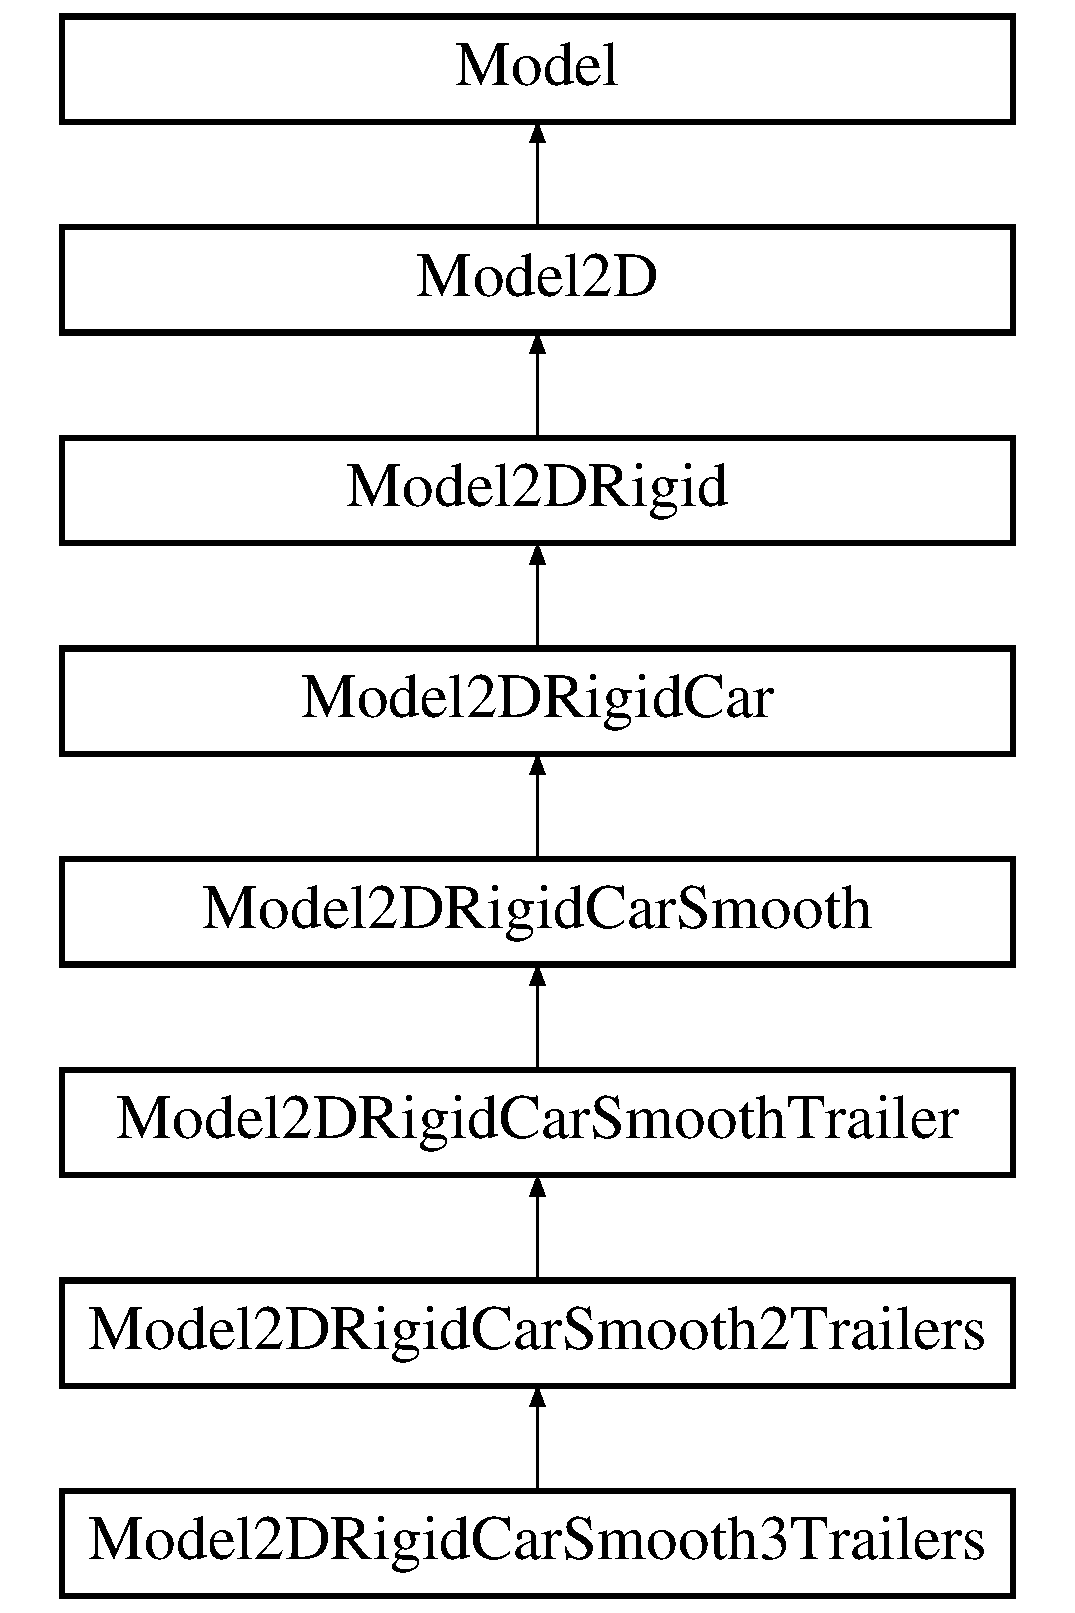
\includegraphics[height=8cm]{classModel2DRigidCarSmooth3Trailers}
\end{center}
\end{figure}
\subsection*{Public Methods}
\begin{CompactItemize}
\item 
{\bf Model2DRigid\-Car\-Smooth3Trailers} (string path)
\item 
virtual {\bf $\sim$Model2DRigid\-Car\-Smooth3Trailers} ()
\item 
virtual {\bf MSLVector} {\bf State\-Transition\-Equation} (const {\bf MSLVector} \&x, const {\bf MSLVector} \&u)
\begin{CompactList}\small\item\em The state transition equation, or equations of motion, xdot=f(x,u).\item\end{CompactList}\item 
virtual double {\bf Metric} (const {\bf MSLVector} \&x1, const {\bf MSLVector} \&x2)
\begin{CompactList}\small\item\em A distance metric, which is Euclidean in the base class.\item\end{CompactList}\item 
virtual {\bf MSLVector} {\bf State\-To\-Configuration} (const {\bf MSLVector} \&x)
\begin{CompactList}\small\item\em A method that converts a {\bf Model} {\rm (p.\,\pageref{classModel})} state in to a {\bf Geom} {\rm (p.\,\pageref{classGeom})} configuration.\item\end{CompactList}\item 
virtual bool {\bf Satisfied} (const {\bf MSLVector} \&x)
\begin{CompactList}\small\item\em Test whether global state-space constraints are satisfied.\item\end{CompactList}\end{CompactItemize}
\subsection*{Public Attributes}
\begin{CompactItemize}
\item 
double {\bf Hitch3Length}
\item 
double {\bf Hitch3Max\-Angle}
\end{CompactItemize}


\subsection{Detailed Description}
A rigid car-like robot with continuous steering angles and three trailers.



\subsection{Constructor \& Destructor Documentation}
\index{Model2DRigidCarSmooth3Trailers@{Model2DRigid\-Car\-Smooth3Trailers}!Model2DRigidCarSmooth3Trailers@{Model2DRigidCarSmooth3Trailers}}
\index{Model2DRigidCarSmooth3Trailers@{Model2DRigidCarSmooth3Trailers}!Model2DRigidCarSmooth3Trailers@{Model2DRigid\-Car\-Smooth3Trailers}}
\subsubsection{\setlength{\rightskip}{0pt plus 5cm}Model2DRigid\-Car\-Smooth3Trailers::Model2DRigid\-Car\-Smooth3Trailers (string {\em path} = \char`\"{}\char`\"{})}\label{classModel2DRigidCarSmooth3Trailers_a0}


\index{Model2DRigidCarSmooth3Trailers@{Model2DRigid\-Car\-Smooth3Trailers}!~Model2DRigidCarSmooth3Trailers@{$\sim$Model2DRigidCarSmooth3Trailers}}
\index{~Model2DRigidCarSmooth3Trailers@{$\sim$Model2DRigidCarSmooth3Trailers}!Model2DRigidCarSmooth3Trailers@{Model2DRigid\-Car\-Smooth3Trailers}}
\subsubsection{\setlength{\rightskip}{0pt plus 5cm}Model2DRigid\-Car\-Smooth3Trailers::$\sim$Model2DRigid\-Car\-Smooth3Trailers ()\hspace{0.3cm}{\tt  [inline, virtual]}}\label{classModel2DRigidCarSmooth3Trailers_a1}




\subsection{Member Function Documentation}
\index{Model2DRigidCarSmooth3Trailers@{Model2DRigid\-Car\-Smooth3Trailers}!Metric@{Metric}}
\index{Metric@{Metric}!Model2DRigidCarSmooth3Trailers@{Model2DRigid\-Car\-Smooth3Trailers}}
\subsubsection{\setlength{\rightskip}{0pt plus 5cm}double Model2DRigid\-Car\-Smooth3Trailers::Metric (const {\bf MSLVector} \& {\em x1}, const {\bf MSLVector} \& {\em x2})\hspace{0.3cm}{\tt  [virtual]}}\label{classModel2DRigidCarSmooth3Trailers_a3}


A distance metric, which is Euclidean in the base class.



Reimplemented from {\bf Model2DRigid\-Car\-Smooth2Trailers} {\rm (p.\,\pageref{classModel2DRigidCarSmooth2Trailers_a3})}.\index{Model2DRigidCarSmooth3Trailers@{Model2DRigid\-Car\-Smooth3Trailers}!Satisfied@{Satisfied}}
\index{Satisfied@{Satisfied}!Model2DRigidCarSmooth3Trailers@{Model2DRigid\-Car\-Smooth3Trailers}}
\subsubsection{\setlength{\rightskip}{0pt plus 5cm}bool Model2DRigid\-Car\-Smooth3Trailers::Satisfied (const {\bf MSLVector} \& {\em x})\hspace{0.3cm}{\tt  [virtual]}}\label{classModel2DRigidCarSmooth3Trailers_a5}


Test whether global state-space constraints are satisfied.



Reimplemented from {\bf Model2DRigid\-Car\-Smooth2Trailers} {\rm (p.\,\pageref{classModel2DRigidCarSmooth2Trailers_a5})}.\index{Model2DRigidCarSmooth3Trailers@{Model2DRigid\-Car\-Smooth3Trailers}!StateToConfiguration@{StateToConfiguration}}
\index{StateToConfiguration@{StateToConfiguration}!Model2DRigidCarSmooth3Trailers@{Model2DRigid\-Car\-Smooth3Trailers}}
\subsubsection{\setlength{\rightskip}{0pt plus 5cm}{\bf MSLVector} Model2DRigid\-Car\-Smooth3Trailers::State\-To\-Configuration (const {\bf MSLVector} \& {\em x})\hspace{0.3cm}{\tt  [virtual]}}\label{classModel2DRigidCarSmooth3Trailers_a4}


A method that converts a {\bf Model} {\rm (p.\,\pageref{classModel})} state in to a {\bf Geom} {\rm (p.\,\pageref{classGeom})} configuration.



Reimplemented from {\bf Model2DRigid\-Car\-Smooth2Trailers} {\rm (p.\,\pageref{classModel2DRigidCarSmooth2Trailers_a4})}.\index{Model2DRigidCarSmooth3Trailers@{Model2DRigid\-Car\-Smooth3Trailers}!StateTransitionEquation@{StateTransitionEquation}}
\index{StateTransitionEquation@{StateTransitionEquation}!Model2DRigidCarSmooth3Trailers@{Model2DRigid\-Car\-Smooth3Trailers}}
\subsubsection{\setlength{\rightskip}{0pt plus 5cm}{\bf MSLVector} Model2DRigid\-Car\-Smooth3Trailers::State\-Transition\-Equation (const {\bf MSLVector} \& {\em x}, const {\bf MSLVector} \& {\em u})\hspace{0.3cm}{\tt  [virtual]}}\label{classModel2DRigidCarSmooth3Trailers_a2}


The state transition equation, or equations of motion, xdot=f(x,u).



Reimplemented from {\bf Model2DRigid\-Car\-Smooth2Trailers} {\rm (p.\,\pageref{classModel2DRigidCarSmooth2Trailers_a2})}.

\subsection{Member Data Documentation}
\index{Model2DRigidCarSmooth3Trailers@{Model2DRigid\-Car\-Smooth3Trailers}!Hitch3Length@{Hitch3Length}}
\index{Hitch3Length@{Hitch3Length}!Model2DRigidCarSmooth3Trailers@{Model2DRigid\-Car\-Smooth3Trailers}}
\subsubsection{\setlength{\rightskip}{0pt plus 5cm}double Model2DRigid\-Car\-Smooth3Trailers::Hitch3Length}\label{classModel2DRigidCarSmooth3Trailers_m0}


\index{Model2DRigidCarSmooth3Trailers@{Model2DRigid\-Car\-Smooth3Trailers}!Hitch3MaxAngle@{Hitch3MaxAngle}}
\index{Hitch3MaxAngle@{Hitch3MaxAngle}!Model2DRigidCarSmooth3Trailers@{Model2DRigid\-Car\-Smooth3Trailers}}
\subsubsection{\setlength{\rightskip}{0pt plus 5cm}double Model2DRigid\-Car\-Smooth3Trailers::Hitch3Max\-Angle}\label{classModel2DRigidCarSmooth3Trailers_m1}




The documentation for this class was generated from the following files:\begin{CompactItemize}
\item 
{\bf model2d.h}\item 
{\bf model2d.C}\end{CompactItemize}

\section{Model2DRigid\-Car\-Smooth\-Trailer  Class Reference}
\label{classModel2DRigidCarSmoothTrailer}\index{Model2DRigidCarSmoothTrailer@{Model2DRigid\-Car\-Smooth\-Trailer}}
A rigid car-like robot with continuous steering angles and a trailer. The trailer models are taken from Murray and Sastry, Trans. Automatic Control, Vol 38, No 5, 1993, pp. 700-716. 


{\tt \#include $<$model2d.h$>$}

Inheritance diagram for Model2DRigid\-Car\-Smooth\-Trailer::\begin{figure}[H]
\begin{center}
\leavevmode
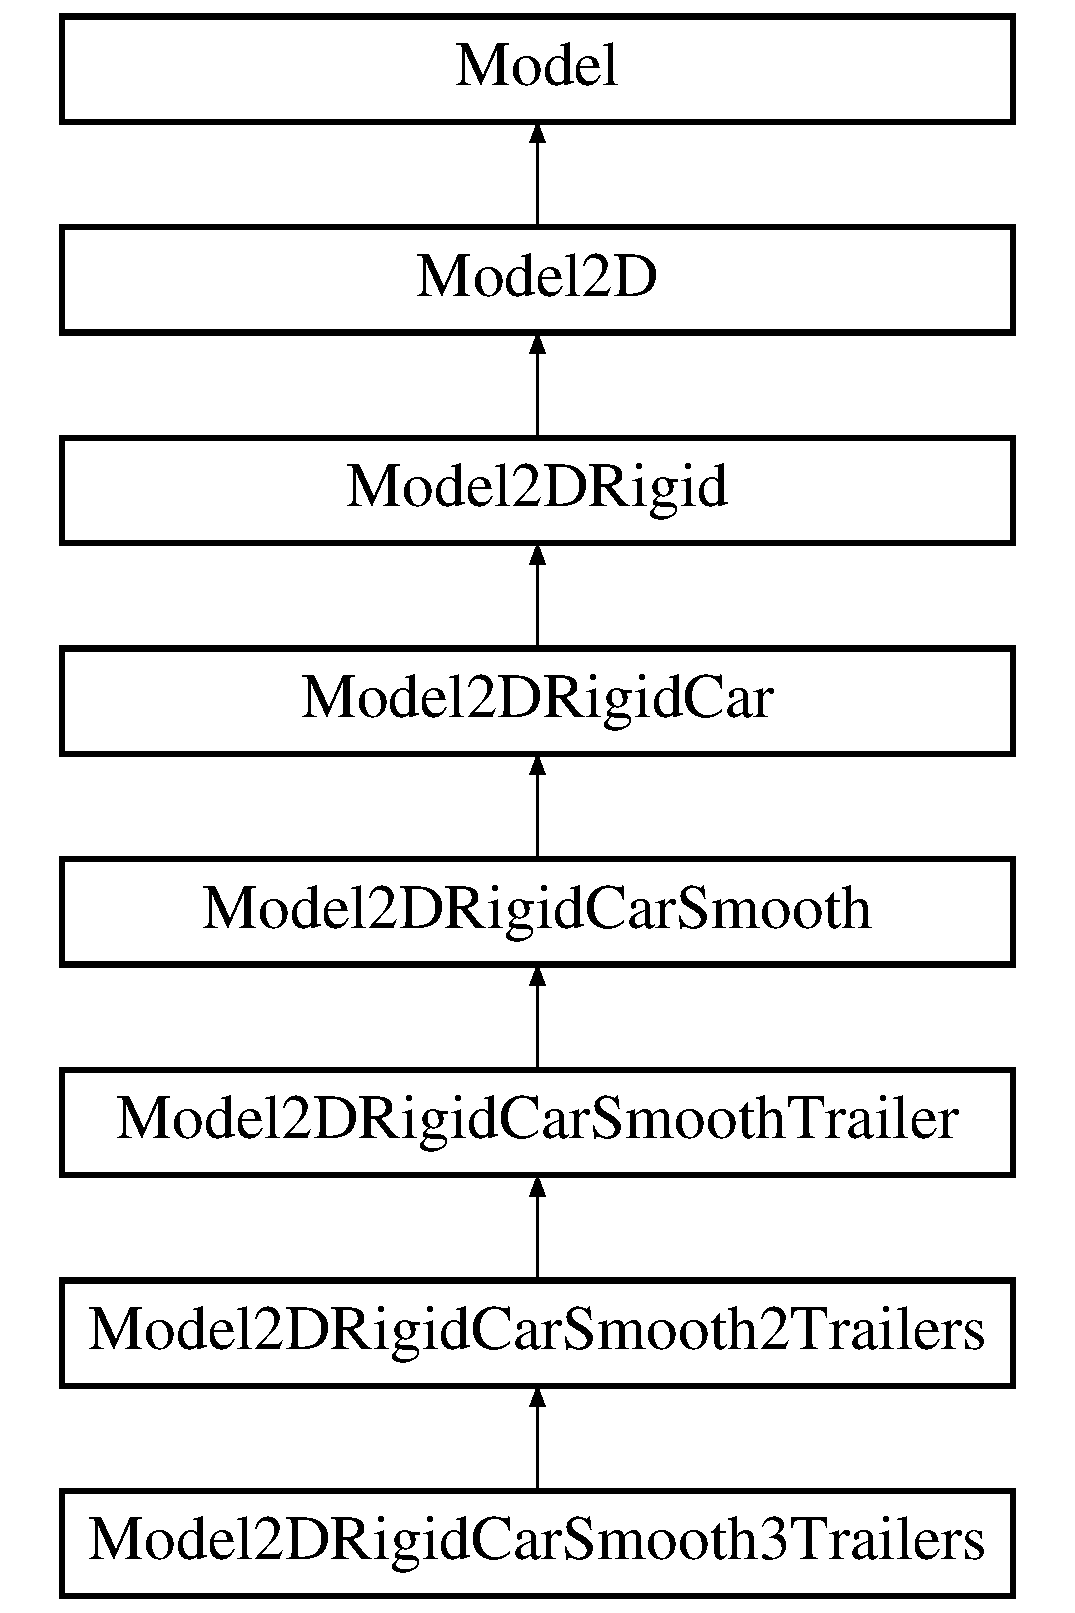
\includegraphics[height=8cm]{classModel2DRigidCarSmoothTrailer}
\end{center}
\end{figure}
\subsection*{Public Methods}
\begin{CompactItemize}
\item 
{\bf Model2DRigid\-Car\-Smooth\-Trailer} (string path)
\item 
virtual {\bf $\sim$Model2DRigid\-Car\-Smooth\-Trailer} ()
\item 
virtual {\bf MSLVector} {\bf State\-Transition\-Equation} (const {\bf MSLVector} \&x, const {\bf MSLVector} \&u)
\begin{CompactList}\small\item\em The state transition equation, or equations of motion, xdot=f(x,u).\item\end{CompactList}\item 
virtual double {\bf Metric} (const {\bf MSLVector} \&x1, const {\bf MSLVector} \&x2)
\begin{CompactList}\small\item\em A distance metric, which is Euclidean in the base class.\item\end{CompactList}\item 
virtual {\bf MSLVector} {\bf State\-To\-Configuration} (const {\bf MSLVector} \&x)
\begin{CompactList}\small\item\em A method that converts a {\bf Model} {\rm (p.\,\pageref{classModel})} state in to a {\bf Geom} {\rm (p.\,\pageref{classGeom})} configuration.\item\end{CompactList}\item 
virtual bool {\bf Satisfied} (const {\bf MSLVector} \&x)
\begin{CompactList}\small\item\em Test whether global state-space constraints are satisfied.\item\end{CompactList}\end{CompactItemize}
\subsection*{Public Attributes}
\begin{CompactItemize}
\item 
double {\bf Hitch\-Length}
\item 
double {\bf Hitch\-Max\-Angle}
\end{CompactItemize}


\subsection{Detailed Description}
A rigid car-like robot with continuous steering angles and a trailer. The trailer models are taken from Murray and Sastry, Trans. Automatic Control, Vol 38, No 5, 1993, pp. 700-716.



\subsection{Constructor \& Destructor Documentation}
\index{Model2DRigidCarSmoothTrailer@{Model2DRigid\-Car\-Smooth\-Trailer}!Model2DRigidCarSmoothTrailer@{Model2DRigidCarSmoothTrailer}}
\index{Model2DRigidCarSmoothTrailer@{Model2DRigidCarSmoothTrailer}!Model2DRigidCarSmoothTrailer@{Model2DRigid\-Car\-Smooth\-Trailer}}
\subsubsection{\setlength{\rightskip}{0pt plus 5cm}Model2DRigid\-Car\-Smooth\-Trailer::Model2DRigid\-Car\-Smooth\-Trailer (string {\em path} = \char`\"{}\char`\"{})}\label{classModel2DRigidCarSmoothTrailer_a0}


\index{Model2DRigidCarSmoothTrailer@{Model2DRigid\-Car\-Smooth\-Trailer}!~Model2DRigidCarSmoothTrailer@{$\sim$Model2DRigidCarSmoothTrailer}}
\index{~Model2DRigidCarSmoothTrailer@{$\sim$Model2DRigidCarSmoothTrailer}!Model2DRigidCarSmoothTrailer@{Model2DRigid\-Car\-Smooth\-Trailer}}
\subsubsection{\setlength{\rightskip}{0pt plus 5cm}Model2DRigid\-Car\-Smooth\-Trailer::$\sim$Model2DRigid\-Car\-Smooth\-Trailer ()\hspace{0.3cm}{\tt  [inline, virtual]}}\label{classModel2DRigidCarSmoothTrailer_a1}




\subsection{Member Function Documentation}
\index{Model2DRigidCarSmoothTrailer@{Model2DRigid\-Car\-Smooth\-Trailer}!Metric@{Metric}}
\index{Metric@{Metric}!Model2DRigidCarSmoothTrailer@{Model2DRigid\-Car\-Smooth\-Trailer}}
\subsubsection{\setlength{\rightskip}{0pt plus 5cm}double Model2DRigid\-Car\-Smooth\-Trailer::Metric (const {\bf MSLVector} \& {\em x1}, const {\bf MSLVector} \& {\em x2})\hspace{0.3cm}{\tt  [virtual]}}\label{classModel2DRigidCarSmoothTrailer_a3}


A distance metric, which is Euclidean in the base class.



Reimplemented from {\bf Model2DRigid\-Car\-Smooth} {\rm (p.\,\pageref{classModel2DRigidCarSmooth_a4})}.

Reimplemented in {\bf Model2DRigid\-Car\-Smooth2Trailers} {\rm (p.\,\pageref{classModel2DRigidCarSmooth2Trailers_a3})}, and {\bf Model2DRigid\-Car\-Smooth3Trailers} {\rm (p.\,\pageref{classModel2DRigidCarSmooth3Trailers_a3})}.\index{Model2DRigidCarSmoothTrailer@{Model2DRigid\-Car\-Smooth\-Trailer}!Satisfied@{Satisfied}}
\index{Satisfied@{Satisfied}!Model2DRigidCarSmoothTrailer@{Model2DRigid\-Car\-Smooth\-Trailer}}
\subsubsection{\setlength{\rightskip}{0pt plus 5cm}bool Model2DRigid\-Car\-Smooth\-Trailer::Satisfied (const {\bf MSLVector} \& {\em x})\hspace{0.3cm}{\tt  [virtual]}}\label{classModel2DRigidCarSmoothTrailer_a5}


Test whether global state-space constraints are satisfied.



Reimplemented from {\bf Model2DRigid\-Car\-Smooth} {\rm (p.\,\pageref{classModel2DRigidCarSmooth_a6})}.

Reimplemented in {\bf Model2DRigid\-Car\-Smooth2Trailers} {\rm (p.\,\pageref{classModel2DRigidCarSmooth2Trailers_a5})}, and {\bf Model2DRigid\-Car\-Smooth3Trailers} {\rm (p.\,\pageref{classModel2DRigidCarSmooth3Trailers_a5})}.\index{Model2DRigidCarSmoothTrailer@{Model2DRigid\-Car\-Smooth\-Trailer}!StateToConfiguration@{StateToConfiguration}}
\index{StateToConfiguration@{StateToConfiguration}!Model2DRigidCarSmoothTrailer@{Model2DRigid\-Car\-Smooth\-Trailer}}
\subsubsection{\setlength{\rightskip}{0pt plus 5cm}{\bf MSLVector} Model2DRigid\-Car\-Smooth\-Trailer::State\-To\-Configuration (const {\bf MSLVector} \& {\em x})\hspace{0.3cm}{\tt  [virtual]}}\label{classModel2DRigidCarSmoothTrailer_a4}


A method that converts a {\bf Model} {\rm (p.\,\pageref{classModel})} state in to a {\bf Geom} {\rm (p.\,\pageref{classGeom})} configuration.



Reimplemented from {\bf Model2DRigid\-Car\-Smooth} {\rm (p.\,\pageref{classModel2DRigidCarSmooth_a5})}.

Reimplemented in {\bf Model2DRigid\-Car\-Smooth2Trailers} {\rm (p.\,\pageref{classModel2DRigidCarSmooth2Trailers_a4})}, and {\bf Model2DRigid\-Car\-Smooth3Trailers} {\rm (p.\,\pageref{classModel2DRigidCarSmooth3Trailers_a4})}.\index{Model2DRigidCarSmoothTrailer@{Model2DRigid\-Car\-Smooth\-Trailer}!StateTransitionEquation@{StateTransitionEquation}}
\index{StateTransitionEquation@{StateTransitionEquation}!Model2DRigidCarSmoothTrailer@{Model2DRigid\-Car\-Smooth\-Trailer}}
\subsubsection{\setlength{\rightskip}{0pt plus 5cm}{\bf MSLVector} Model2DRigid\-Car\-Smooth\-Trailer::State\-Transition\-Equation (const {\bf MSLVector} \& {\em x}, const {\bf MSLVector} \& {\em u})\hspace{0.3cm}{\tt  [virtual]}}\label{classModel2DRigidCarSmoothTrailer_a2}


The state transition equation, or equations of motion, xdot=f(x,u).



Reimplemented from {\bf Model2DRigid\-Car\-Smooth} {\rm (p.\,\pageref{classModel2DRigidCarSmooth_a2})}.

Reimplemented in {\bf Model2DRigid\-Car\-Smooth2Trailers} {\rm (p.\,\pageref{classModel2DRigidCarSmooth2Trailers_a2})}, and {\bf Model2DRigid\-Car\-Smooth3Trailers} {\rm (p.\,\pageref{classModel2DRigidCarSmooth3Trailers_a2})}.

\subsection{Member Data Documentation}
\index{Model2DRigidCarSmoothTrailer@{Model2DRigid\-Car\-Smooth\-Trailer}!HitchLength@{HitchLength}}
\index{HitchLength@{HitchLength}!Model2DRigidCarSmoothTrailer@{Model2DRigid\-Car\-Smooth\-Trailer}}
\subsubsection{\setlength{\rightskip}{0pt plus 5cm}double Model2DRigid\-Car\-Smooth\-Trailer::Hitch\-Length}\label{classModel2DRigidCarSmoothTrailer_m0}


\index{Model2DRigidCarSmoothTrailer@{Model2DRigid\-Car\-Smooth\-Trailer}!HitchMaxAngle@{HitchMaxAngle}}
\index{HitchMaxAngle@{HitchMaxAngle}!Model2DRigidCarSmoothTrailer@{Model2DRigid\-Car\-Smooth\-Trailer}}
\subsubsection{\setlength{\rightskip}{0pt plus 5cm}double Model2DRigid\-Car\-Smooth\-Trailer::Hitch\-Max\-Angle}\label{classModel2DRigidCarSmoothTrailer_m1}




The documentation for this class was generated from the following files:\begin{CompactItemize}
\item 
{\bf model2d.h}\item 
{\bf model2d.C}\end{CompactItemize}

\section{Model2DRigid\-Chain  Class Reference}
\label{classModel2DRigidChain}\index{Model2DRigidChain@{Model2DRigid\-Chain}}
A 2D kinematic chain of bodies. 


{\tt \#include $<$model2d.h$>$}

Inheritance diagram for Model2DRigid\-Chain::\begin{figure}[H]
\begin{center}
\leavevmode
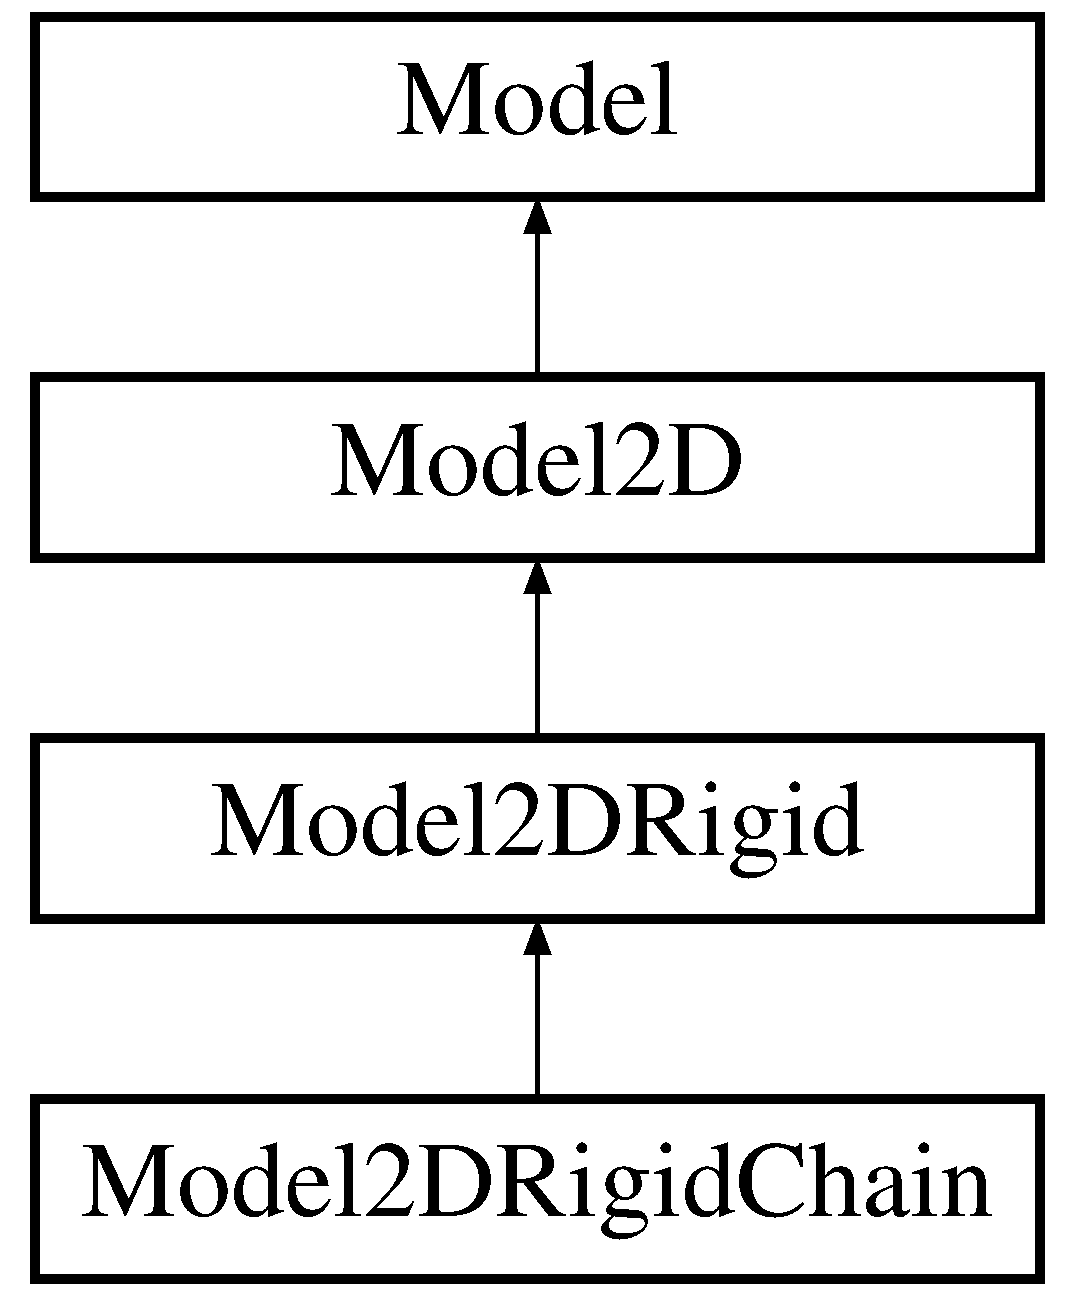
\includegraphics[height=4cm]{classModel2DRigidChain}
\end{center}
\end{figure}
\subsection*{Public Methods}
\begin{CompactItemize}
\item 
{\bf Model2DRigid\-Chain} (string path)
\item 
virtual {\bf $\sim$Model2DRigid\-Chain} ()
\item 
virtual {\bf MSLVector} {\bf State\-To\-Configuration} (const {\bf MSLVector} \&x)
\begin{CompactList}\small\item\em A method that converts a {\bf Model} {\rm (p.\,\pageref{classModel})} state in to a {\bf Geom} {\rm (p.\,\pageref{classGeom})} configuration.\item\end{CompactList}\item 
virtual {\bf MSLVector} {\bf State\-Transition\-Equation} (const {\bf MSLVector} \&x, const {\bf MSLVector} \&u)
\begin{CompactList}\small\item\em The state transition equation, or equations of motion, xdot=f(x,u).\item\end{CompactList}\item 
virtual {\bf MSLVector} {\bf Linear\-Interpolate} (const {\bf MSLVector} \&x1, const {\bf MSLVector} \&x2, const double \&a)
\begin{CompactList}\small\item\em Linearly interpolate two state while respecting topology.\item\end{CompactList}\item 
virtual double {\bf Metric} (const {\bf MSLVector} \&x1, const {\bf MSLVector} \&x2)
\begin{CompactList}\small\item\em A distance metric, which is Euclidean in the base class.\item\end{CompactList}\item 
virtual bool {\bf Satisfied} (const {\bf MSLVector} \&x)
\begin{CompactList}\small\item\em Test whether global state-space constraints are satisfied.\item\end{CompactList}\end{CompactItemize}
\subsection*{Public Attributes}
\begin{CompactItemize}
\item 
int {\bf Num\-Bodies}
\begin{CompactList}\small\item\em Number of bodies in the chain.\item\end{CompactList}\item 
{\bf MSLVector} {\bf A}
\begin{CompactList}\small\item\em The distances between joints (\char`\"{}a\char`\"{} parameters in kinematics).\item\end{CompactList}\item 
double {\bf Stop\-Angle}
\begin{CompactList}\small\item\em The default joint limits (must be in 0,PI).\item\end{CompactList}\end{CompactItemize}


\subsection{Detailed Description}
A 2D kinematic chain of bodies.



\subsection{Constructor \& Destructor Documentation}
\index{Model2DRigidChain@{Model2DRigid\-Chain}!Model2DRigidChain@{Model2DRigidChain}}
\index{Model2DRigidChain@{Model2DRigidChain}!Model2DRigidChain@{Model2DRigid\-Chain}}
\subsubsection{\setlength{\rightskip}{0pt plus 5cm}Model2DRigid\-Chain::Model2DRigid\-Chain (string {\em path} = \char`\"{}\char`\"{})}\label{classModel2DRigidChain_a0}


\index{Model2DRigidChain@{Model2DRigid\-Chain}!~Model2DRigidChain@{$\sim$Model2DRigidChain}}
\index{~Model2DRigidChain@{$\sim$Model2DRigidChain}!Model2DRigidChain@{Model2DRigid\-Chain}}
\subsubsection{\setlength{\rightskip}{0pt plus 5cm}Model2DRigid\-Chain::$\sim$Model2DRigid\-Chain ()\hspace{0.3cm}{\tt  [inline, virtual]}}\label{classModel2DRigidChain_a1}




\subsection{Member Function Documentation}
\index{Model2DRigidChain@{Model2DRigid\-Chain}!LinearInterpolate@{LinearInterpolate}}
\index{LinearInterpolate@{LinearInterpolate}!Model2DRigidChain@{Model2DRigid\-Chain}}
\subsubsection{\setlength{\rightskip}{0pt plus 5cm}{\bf MSLVector} Model2DRigid\-Chain::Linear\-Interpolate (const {\bf MSLVector} \& {\em x1}, const {\bf MSLVector} \& {\em x2}, const double \& {\em a})\hspace{0.3cm}{\tt  [virtual]}}\label{classModel2DRigidChain_a4}


Linearly interpolate two state while respecting topology.

If a=0, then x1 is returned; if a=1, then x2 is returned. All intermediate values of \$a $\backslash$in [0,1]\$ yield intermediate states. This method is defined by {\bf Model} {\rm (p.\,\pageref{classModel})}. 

Reimplemented from {\bf Model2DRigid} {\rm (p.\,\pageref{classModel2DRigid_a4})}.\index{Model2DRigidChain@{Model2DRigid\-Chain}!Metric@{Metric}}
\index{Metric@{Metric}!Model2DRigidChain@{Model2DRigid\-Chain}}
\subsubsection{\setlength{\rightskip}{0pt plus 5cm}double Model2DRigid\-Chain::Metric (const {\bf MSLVector} \& {\em x1}, const {\bf MSLVector} \& {\em x2})\hspace{0.3cm}{\tt  [virtual]}}\label{classModel2DRigidChain_a5}


A distance metric, which is Euclidean in the base class.



Reimplemented from {\bf Model2DRigid} {\rm (p.\,\pageref{classModel2DRigid_a5})}.\index{Model2DRigidChain@{Model2DRigid\-Chain}!Satisfied@{Satisfied}}
\index{Satisfied@{Satisfied}!Model2DRigidChain@{Model2DRigid\-Chain}}
\subsubsection{\setlength{\rightskip}{0pt plus 5cm}bool Model2DRigid\-Chain::Satisfied (const {\bf MSLVector} \& {\em x})\hspace{0.3cm}{\tt  [virtual]}}\label{classModel2DRigidChain_a6}


Test whether global state-space constraints are satisfied.



Reimplemented from {\bf Model} {\rm (p.\,\pageref{classModel_a4})}.\index{Model2DRigidChain@{Model2DRigid\-Chain}!StateToConfiguration@{StateToConfiguration}}
\index{StateToConfiguration@{StateToConfiguration}!Model2DRigidChain@{Model2DRigid\-Chain}}
\subsubsection{\setlength{\rightskip}{0pt plus 5cm}{\bf MSLVector} Model2DRigid\-Chain::State\-To\-Configuration (const {\bf MSLVector} \& {\em x})\hspace{0.3cm}{\tt  [virtual]}}\label{classModel2DRigidChain_a2}


A method that converts a {\bf Model} {\rm (p.\,\pageref{classModel})} state in to a {\bf Geom} {\rm (p.\,\pageref{classGeom})} configuration.



Reimplemented from {\bf Model2DRigid} {\rm (p.\,\pageref{classModel2DRigid_a6})}.\index{Model2DRigidChain@{Model2DRigid\-Chain}!StateTransitionEquation@{StateTransitionEquation}}
\index{StateTransitionEquation@{StateTransitionEquation}!Model2DRigidChain@{Model2DRigid\-Chain}}
\subsubsection{\setlength{\rightskip}{0pt plus 5cm}{\bf MSLVector} Model2DRigid\-Chain::State\-Transition\-Equation (const {\bf MSLVector} \& {\em x}, const {\bf MSLVector} \& {\em u})\hspace{0.3cm}{\tt  [virtual]}}\label{classModel2DRigidChain_a3}


The state transition equation, or equations of motion, xdot=f(x,u).



Reimplemented from {\bf Model2DRigid} {\rm (p.\,\pageref{classModel2DRigid_a3})}.

\subsection{Member Data Documentation}
\index{Model2DRigidChain@{Model2DRigid\-Chain}!A@{A}}
\index{A@{A}!Model2DRigidChain@{Model2DRigid\-Chain}}
\subsubsection{\setlength{\rightskip}{0pt plus 5cm}{\bf MSLVector} Model2DRigid\-Chain::A}\label{classModel2DRigidChain_m1}


The distances between joints (\char`\"{}a\char`\"{} parameters in kinematics).

\index{Model2DRigidChain@{Model2DRigid\-Chain}!NumBodies@{NumBodies}}
\index{NumBodies@{NumBodies}!Model2DRigidChain@{Model2DRigid\-Chain}}
\subsubsection{\setlength{\rightskip}{0pt plus 5cm}int Model2DRigid\-Chain::Num\-Bodies}\label{classModel2DRigidChain_m0}


Number of bodies in the chain.

\index{Model2DRigidChain@{Model2DRigid\-Chain}!StopAngle@{StopAngle}}
\index{StopAngle@{StopAngle}!Model2DRigidChain@{Model2DRigid\-Chain}}
\subsubsection{\setlength{\rightskip}{0pt plus 5cm}double Model2DRigid\-Chain::Stop\-Angle}\label{classModel2DRigidChain_m2}


The default joint limits (must be in 0,PI).



The documentation for this class was generated from the following files:\begin{CompactItemize}
\item 
{\bf model2d.h}\item 
{\bf model2d.C}\end{CompactItemize}

\section{Model2DRigid\-Dyncar  Class Reference}
\label{classModel2DRigidDyncar}\index{Model2DRigidDyncar@{Model2DRigid\-Dyncar}}
A 5DOF dynamical model of a rigid car. This model uses a linear tire model, which is far from reality. The model was donated by Jim Bernard. 


{\tt \#include $<$model2d.h$>$}

Inheritance diagram for Model2DRigid\-Dyncar::\begin{figure}[H]
\begin{center}
\leavevmode
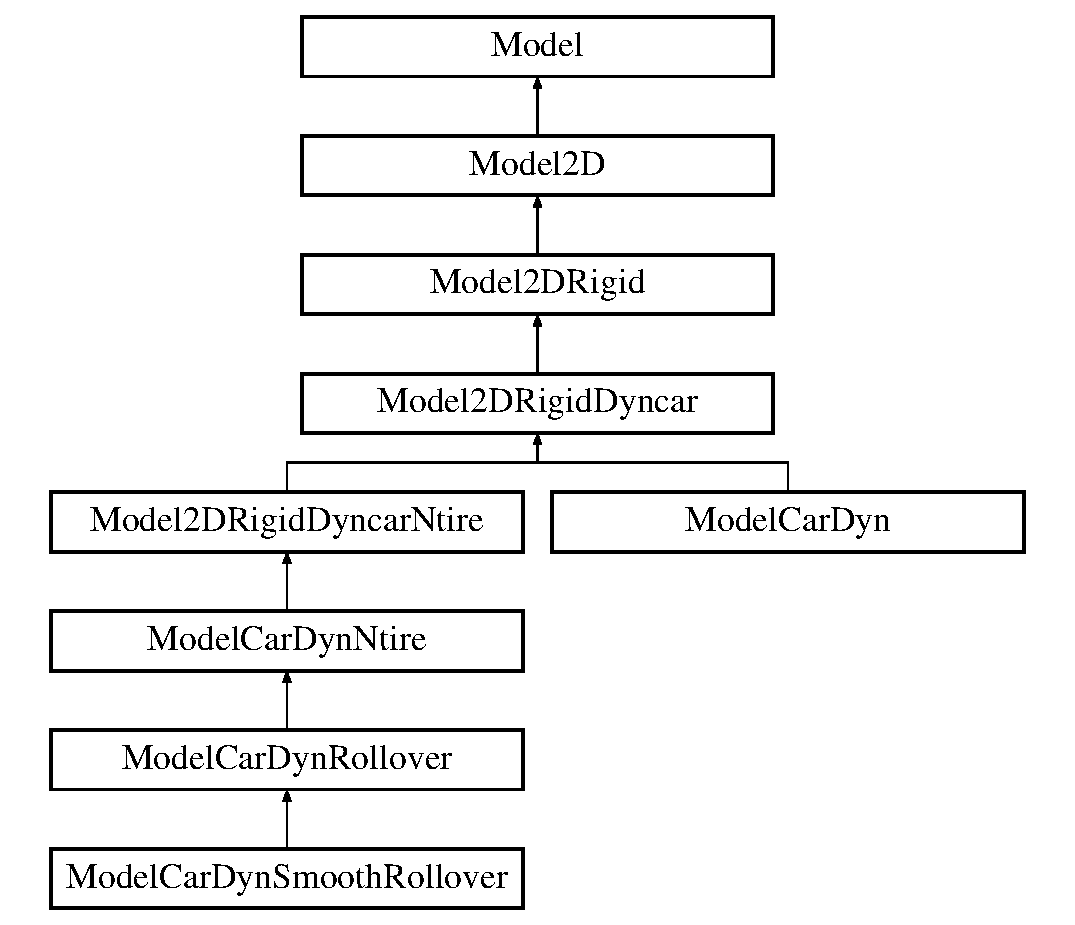
\includegraphics[height=8cm]{classModel2DRigidDyncar}
\end{center}
\end{figure}
\subsection*{Public Methods}
\begin{CompactItemize}
\item 
{\bf Model2DRigid\-Dyncar} (string path)
\item 
virtual {\bf $\sim$Model2DRigid\-Dyncar} ()
\item 
{\bf MSLVector} {\bf Integrate} (const {\bf MSLVector} \&x, const {\bf MSLVector} \&u, const double \&h)
\begin{CompactList}\small\item\em Perform integration from state x, using input u, over time step h.\item\end{CompactList}\item 
virtual {\bf MSLVector} {\bf State\-To\-Configuration} (const {\bf MSLVector} \&x)
\begin{CompactList}\small\item\em A method that converts a {\bf Model} {\rm (p.\,\pageref{classModel})} state in to a {\bf Geom} {\rm (p.\,\pageref{classGeom})} configuration.\item\end{CompactList}\item 
virtual {\bf MSLVector} {\bf State\-Transition\-Equation} (const {\bf MSLVector} \&x, const {\bf MSLVector} \&u)
\begin{CompactList}\small\item\em The state transition equation, or equations of motion, xdot=f(x,u).\item\end{CompactList}\item 
virtual double {\bf Metric} (const {\bf MSLVector} \&x1, const {\bf MSLVector} \&x2)
\begin{CompactList}\small\item\em A distance metric, which is Euclidean in the base class.\item\end{CompactList}\item 
virtual {\bf MSLVector} {\bf Linear\-Interpolate} (const {\bf MSLVector} \&x1, const {\bf MSLVector} \&x2, const double \&a)
\begin{CompactList}\small\item\em Linearly interpolate two state while respecting topology.\item\end{CompactList}\end{CompactItemize}
\subsection*{Public Attributes}
\begin{CompactItemize}
\item 
double {\bf Mass}
\begin{CompactList}\small\item\em Mass in slugs (yuck! American customary units...).\item\end{CompactList}\item 
double {\bf CAF}
\begin{CompactList}\small\item\em Front cornering stiffness.\item\end{CompactList}\item 
double {\bf CAR}
\begin{CompactList}\small\item\em Rear cornering stiffness.\item\end{CompactList}\item 
double {\bf Adist}
\begin{CompactList}\small\item\em Mass center to front tires - feet.\item\end{CompactList}\item 
double {\bf Bdist}
\begin{CompactList}\small\item\em Mass center to rear tires - feet.\item\end{CompactList}\item 
double {\bf Izz}
\begin{CompactList}\small\item\em Yaw moment of interia - ft slugs$^\wedge$2.\item\end{CompactList}\item 
double {\bf World\-Scale}
\begin{CompactList}\small\item\em Feet per world unit (100x100 world).\item\end{CompactList}\item 
double {\bf Max\-Steering\-Angle}
\begin{CompactList}\small\item\em Maximum steering angle in radians.\item\end{CompactList}\item 
double {\bf Speed}
\begin{CompactList}\small\item\em A forward speed of the car.\item\end{CompactList}\end{CompactItemize}


\subsection{Detailed Description}
A 5DOF dynamical model of a rigid car. This model uses a linear tire model, which is far from reality. The model was donated by Jim Bernard.



\subsection{Constructor \& Destructor Documentation}
\index{Model2DRigidDyncar@{Model2DRigid\-Dyncar}!Model2DRigidDyncar@{Model2DRigidDyncar}}
\index{Model2DRigidDyncar@{Model2DRigidDyncar}!Model2DRigidDyncar@{Model2DRigid\-Dyncar}}
\subsubsection{\setlength{\rightskip}{0pt plus 5cm}Model2DRigid\-Dyncar::Model2DRigid\-Dyncar (string {\em path} = \char`\"{}\char`\"{})}\label{classModel2DRigidDyncar_a0}


\index{Model2DRigidDyncar@{Model2DRigid\-Dyncar}!~Model2DRigidDyncar@{$\sim$Model2DRigidDyncar}}
\index{~Model2DRigidDyncar@{$\sim$Model2DRigidDyncar}!Model2DRigidDyncar@{Model2DRigid\-Dyncar}}
\subsubsection{\setlength{\rightskip}{0pt plus 5cm}Model2DRigid\-Dyncar::$\sim$Model2DRigid\-Dyncar ()\hspace{0.3cm}{\tt  [inline, virtual]}}\label{classModel2DRigidDyncar_a1}




\subsection{Member Function Documentation}
\index{Model2DRigidDyncar@{Model2DRigid\-Dyncar}!Integrate@{Integrate}}
\index{Integrate@{Integrate}!Model2DRigidDyncar@{Model2DRigid\-Dyncar}}
\subsubsection{\setlength{\rightskip}{0pt plus 5cm}{\bf MSLVector} Model2DRigid\-Dyncar::Integrate (const {\bf MSLVector} \& {\em x}, const {\bf MSLVector} \& {\em u}, const double \& {\em h})\hspace{0.3cm}{\tt  [virtual]}}\label{classModel2DRigidDyncar_a2}


Perform integration from state x, using input u, over time step h.



Reimplemented from {\bf Model2DRigid} {\rm (p.\,\pageref{classModel2DRigid_a2})}.

Reimplemented in {\bf Model\-Car\-Dyn\-Rollover} {\rm (p.\,\pageref{classModelCarDynRollover_a5})}.\index{Model2DRigidDyncar@{Model2DRigid\-Dyncar}!LinearInterpolate@{LinearInterpolate}}
\index{LinearInterpolate@{LinearInterpolate}!Model2DRigidDyncar@{Model2DRigid\-Dyncar}}
\subsubsection{\setlength{\rightskip}{0pt plus 5cm}{\bf MSLVector} Model2DRigid\-Dyncar::Linear\-Interpolate (const {\bf MSLVector} \& {\em x1}, const {\bf MSLVector} \& {\em x2}, const double \& {\em a})\hspace{0.3cm}{\tt  [virtual]}}\label{classModel2DRigidDyncar_a6}


Linearly interpolate two state while respecting topology.

If a=0, then x1 is returned; if a=1, then x2 is returned. All intermediate values of \$a $\backslash$in [0,1]\$ yield intermediate states. This method is defined by {\bf Model} {\rm (p.\,\pageref{classModel})}. 

Reimplemented from {\bf Model2DRigid} {\rm (p.\,\pageref{classModel2DRigid_a4})}.

Reimplemented in {\bf Model\-Car\-Dyn\-Smooth\-Rollover} {\rm (p.\,\pageref{classModelCarDynSmoothRollover_a5})}.\index{Model2DRigidDyncar@{Model2DRigid\-Dyncar}!Metric@{Metric}}
\index{Metric@{Metric}!Model2DRigidDyncar@{Model2DRigid\-Dyncar}}
\subsubsection{\setlength{\rightskip}{0pt plus 5cm}double Model2DRigid\-Dyncar::Metric (const {\bf MSLVector} \& {\em x1}, const {\bf MSLVector} \& {\em x2})\hspace{0.3cm}{\tt  [virtual]}}\label{classModel2DRigidDyncar_a5}


A distance metric, which is Euclidean in the base class.



Reimplemented from {\bf Model2DRigid} {\rm (p.\,\pageref{classModel2DRigid_a5})}.

Reimplemented in {\bf Model\-Car\-Dyn} {\rm (p.\,\pageref{classModelCarDyn_a3})}, {\bf Model\-Car\-Dyn\-Ntire} {\rm (p.\,\pageref{classModelCarDynNtire_a3})}, {\bf Model\-Car\-Dyn\-Rollover} {\rm (p.\,\pageref{classModelCarDynRollover_a6})}, and {\bf Model\-Car\-Dyn\-Smooth\-Rollover} {\rm (p.\,\pageref{classModelCarDynSmoothRollover_a4})}.\index{Model2DRigidDyncar@{Model2DRigid\-Dyncar}!StateToConfiguration@{StateToConfiguration}}
\index{StateToConfiguration@{StateToConfiguration}!Model2DRigidDyncar@{Model2DRigid\-Dyncar}}
\subsubsection{\setlength{\rightskip}{0pt plus 5cm}{\bf MSLVector} Model2DRigid\-Dyncar::State\-To\-Configuration (const {\bf MSLVector} \& {\em x})\hspace{0.3cm}{\tt  [virtual]}}\label{classModel2DRigidDyncar_a3}


A method that converts a {\bf Model} {\rm (p.\,\pageref{classModel})} state in to a {\bf Geom} {\rm (p.\,\pageref{classGeom})} configuration.



Reimplemented from {\bf Model2DRigid} {\rm (p.\,\pageref{classModel2DRigid_a6})}.

Reimplemented in {\bf Model\-Car\-Dyn} {\rm (p.\,\pageref{classModelCarDyn_a2})}, {\bf Model\-Car\-Dyn\-Ntire} {\rm (p.\,\pageref{classModelCarDynNtire_a2})}, {\bf Model\-Car\-Dyn\-Rollover} {\rm (p.\,\pageref{classModelCarDynRollover_a4})}, and {\bf Model\-Car\-Dyn\-Smooth\-Rollover} {\rm (p.\,\pageref{classModelCarDynSmoothRollover_a3})}.\index{Model2DRigidDyncar@{Model2DRigid\-Dyncar}!StateTransitionEquation@{StateTransitionEquation}}
\index{StateTransitionEquation@{StateTransitionEquation}!Model2DRigidDyncar@{Model2DRigid\-Dyncar}}
\subsubsection{\setlength{\rightskip}{0pt plus 5cm}{\bf MSLVector} Model2DRigid\-Dyncar::State\-Transition\-Equation (const {\bf MSLVector} \& {\em x1}, const {\bf MSLVector} \& {\em u})\hspace{0.3cm}{\tt  [virtual]}}\label{classModel2DRigidDyncar_a4}


The state transition equation, or equations of motion, xdot=f(x,u).



Reimplemented from {\bf Model2DRigid} {\rm (p.\,\pageref{classModel2DRigid_a3})}.

Reimplemented in {\bf Model2DRigid\-Dyncar\-Ntire} {\rm (p.\,\pageref{classModel2DRigidDyncarNtire_a2})}, {\bf Model\-Car\-Dyn\-Rollover} {\rm (p.\,\pageref{classModelCarDynRollover_a3})}, and {\bf Model\-Car\-Dyn\-Smooth\-Rollover} {\rm (p.\,\pageref{classModelCarDynSmoothRollover_a2})}.

\subsection{Member Data Documentation}
\index{Model2DRigidDyncar@{Model2DRigid\-Dyncar}!Adist@{Adist}}
\index{Adist@{Adist}!Model2DRigidDyncar@{Model2DRigid\-Dyncar}}
\subsubsection{\setlength{\rightskip}{0pt plus 5cm}double Model2DRigid\-Dyncar::Adist}\label{classModel2DRigidDyncar_m3}


Mass center to front tires - feet.

\index{Model2DRigidDyncar@{Model2DRigid\-Dyncar}!Bdist@{Bdist}}
\index{Bdist@{Bdist}!Model2DRigidDyncar@{Model2DRigid\-Dyncar}}
\subsubsection{\setlength{\rightskip}{0pt plus 5cm}double Model2DRigid\-Dyncar::Bdist}\label{classModel2DRigidDyncar_m4}


Mass center to rear tires - feet.

\index{Model2DRigidDyncar@{Model2DRigid\-Dyncar}!CAF@{CAF}}
\index{CAF@{CAF}!Model2DRigidDyncar@{Model2DRigid\-Dyncar}}
\subsubsection{\setlength{\rightskip}{0pt plus 5cm}double Model2DRigid\-Dyncar::CAF}\label{classModel2DRigidDyncar_m1}


Front cornering stiffness.

\index{Model2DRigidDyncar@{Model2DRigid\-Dyncar}!CAR@{CAR}}
\index{CAR@{CAR}!Model2DRigidDyncar@{Model2DRigid\-Dyncar}}
\subsubsection{\setlength{\rightskip}{0pt plus 5cm}double Model2DRigid\-Dyncar::CAR}\label{classModel2DRigidDyncar_m2}


Rear cornering stiffness.

\index{Model2DRigidDyncar@{Model2DRigid\-Dyncar}!Izz@{Izz}}
\index{Izz@{Izz}!Model2DRigidDyncar@{Model2DRigid\-Dyncar}}
\subsubsection{\setlength{\rightskip}{0pt plus 5cm}double Model2DRigid\-Dyncar::Izz}\label{classModel2DRigidDyncar_m5}


Yaw moment of interia - ft slugs$^\wedge$2.

\index{Model2DRigidDyncar@{Model2DRigid\-Dyncar}!Mass@{Mass}}
\index{Mass@{Mass}!Model2DRigidDyncar@{Model2DRigid\-Dyncar}}
\subsubsection{\setlength{\rightskip}{0pt plus 5cm}double Model2DRigid\-Dyncar::Mass}\label{classModel2DRigidDyncar_m0}


Mass in slugs (yuck! American customary units...).

\index{Model2DRigidDyncar@{Model2DRigid\-Dyncar}!MaxSteeringAngle@{MaxSteeringAngle}}
\index{MaxSteeringAngle@{MaxSteeringAngle}!Model2DRigidDyncar@{Model2DRigid\-Dyncar}}
\subsubsection{\setlength{\rightskip}{0pt plus 5cm}double Model2DRigid\-Dyncar::Max\-Steering\-Angle}\label{classModel2DRigidDyncar_m7}


Maximum steering angle in radians.

\index{Model2DRigidDyncar@{Model2DRigid\-Dyncar}!Speed@{Speed}}
\index{Speed@{Speed}!Model2DRigidDyncar@{Model2DRigid\-Dyncar}}
\subsubsection{\setlength{\rightskip}{0pt plus 5cm}double Model2DRigid\-Dyncar::Speed}\label{classModel2DRigidDyncar_m8}


A forward speed of the car.

\index{Model2DRigidDyncar@{Model2DRigid\-Dyncar}!WorldScale@{WorldScale}}
\index{WorldScale@{WorldScale}!Model2DRigidDyncar@{Model2DRigid\-Dyncar}}
\subsubsection{\setlength{\rightskip}{0pt plus 5cm}double Model2DRigid\-Dyncar::World\-Scale}\label{classModel2DRigidDyncar_m6}


Feet per world unit (100x100 world).



The documentation for this class was generated from the following files:\begin{CompactItemize}
\item 
{\bf model2d.h}\item 
{\bf model2d.C}\end{CompactItemize}

\section{Model2DRigid\-Dyncar\-Ntire  Class Reference}
\label{classModel2DRigidDyncarNtire}\index{Model2DRigidDyncarNtire@{Model2DRigid\-Dyncar\-Ntire}}
A 5DOF dynamical model of a rigid car. This model uses a nonlinear tire model. The model was donated by Jim Bernard. 


{\tt \#include $<$model2d.h$>$}

Inheritance diagram for Model2DRigid\-Dyncar\-Ntire::\begin{figure}[H]
\begin{center}
\leavevmode
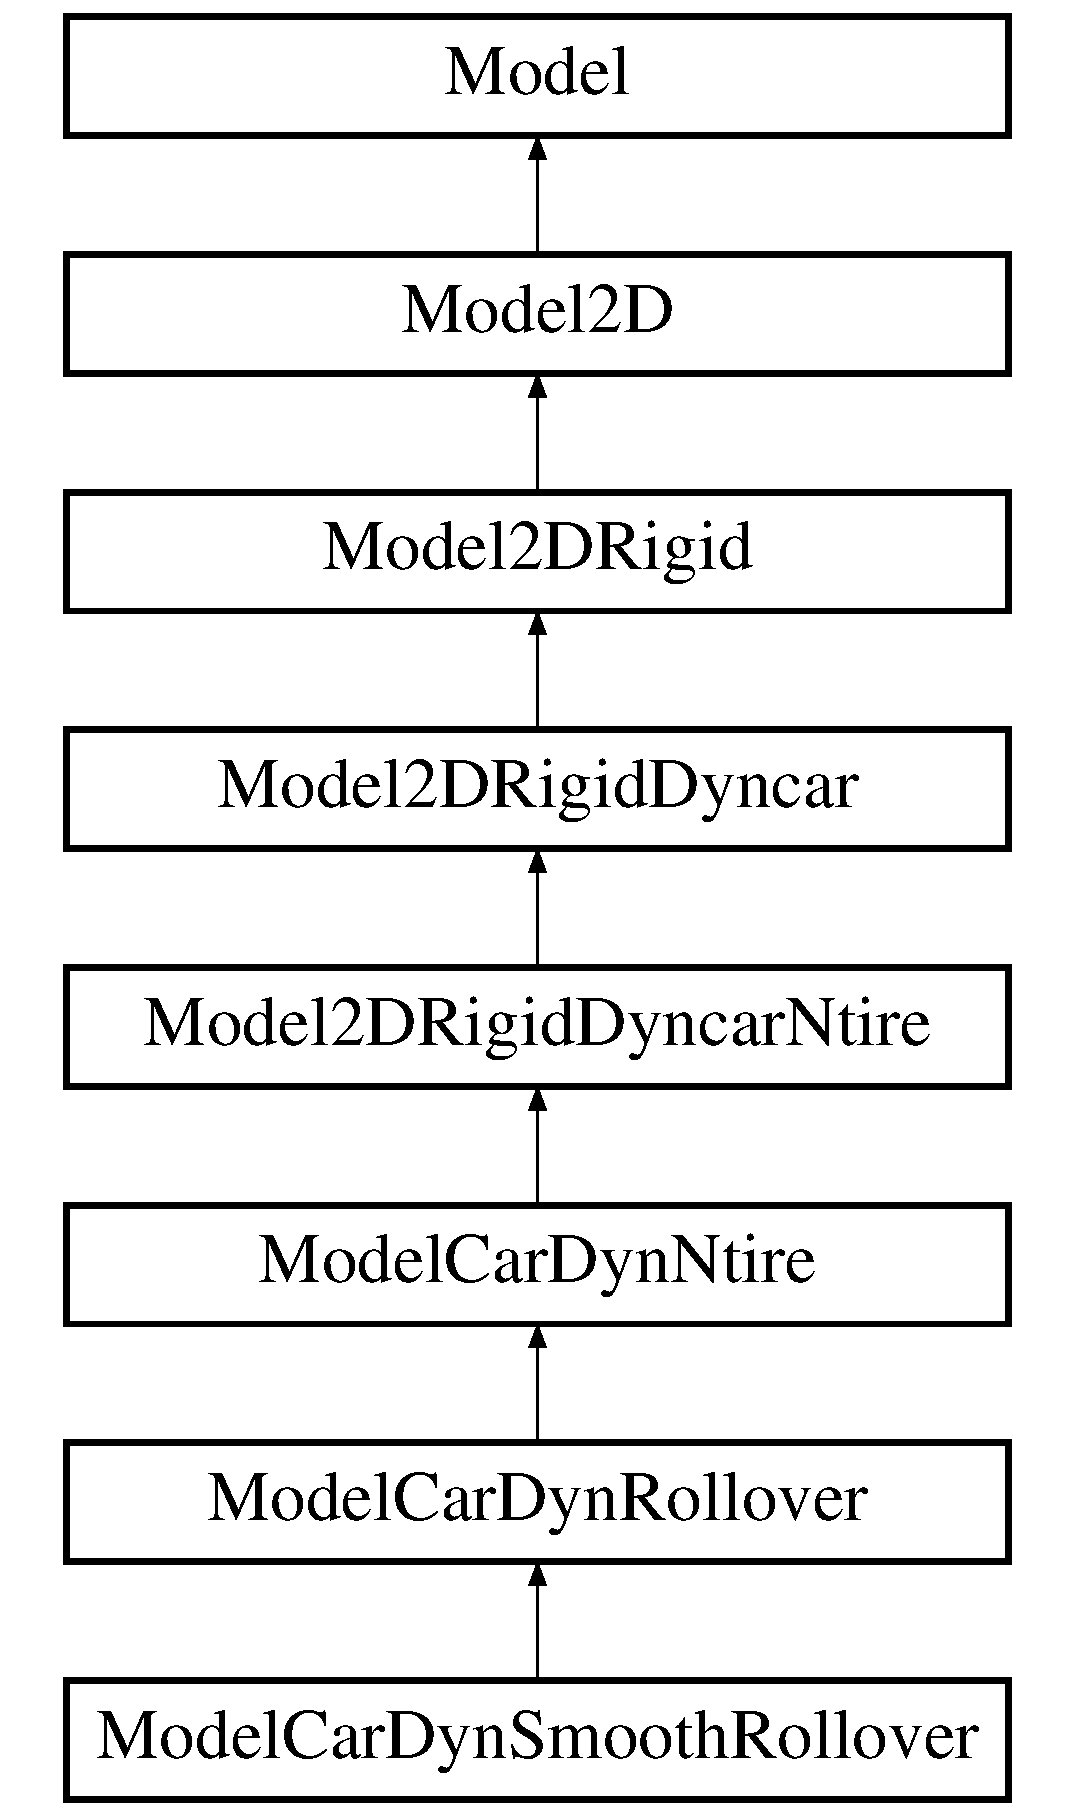
\includegraphics[height=8cm]{classModel2DRigidDyncarNtire}
\end{center}
\end{figure}
\subsection*{Public Methods}
\begin{CompactItemize}
\item 
{\bf Model2DRigid\-Dyncar\-Ntire} (string path)
\item 
virtual {\bf $\sim$Model2DRigid\-Dyncar\-Ntire} ()
\item 
virtual {\bf MSLVector} {\bf State\-Transition\-Equation} (const {\bf MSLVector} \&x, const {\bf MSLVector} \&u)
\begin{CompactList}\small\item\em The state transition equation, or equations of motion, xdot=f(x,u).\item\end{CompactList}\end{CompactItemize}
\subsection*{Public Attributes}
\begin{CompactItemize}
\item 
double {\bf Mu}
\begin{CompactList}\small\item\em Nonlinear tire model constant.\item\end{CompactList}\item 
double {\bf Nf}
\begin{CompactList}\small\item\em Load on the front tires.\item\end{CompactList}\item 
double {\bf Nr}
\begin{CompactList}\small\item\em Load on the rear tires.\item\end{CompactList}\end{CompactItemize}


\subsection{Detailed Description}
A 5DOF dynamical model of a rigid car. This model uses a nonlinear tire model. The model was donated by Jim Bernard.



\subsection{Constructor \& Destructor Documentation}
\index{Model2DRigidDyncarNtire@{Model2DRigid\-Dyncar\-Ntire}!Model2DRigidDyncarNtire@{Model2DRigidDyncarNtire}}
\index{Model2DRigidDyncarNtire@{Model2DRigidDyncarNtire}!Model2DRigidDyncarNtire@{Model2DRigid\-Dyncar\-Ntire}}
\subsubsection{\setlength{\rightskip}{0pt plus 5cm}Model2DRigid\-Dyncar\-Ntire::Model2DRigid\-Dyncar\-Ntire (string {\em path} = \char`\"{}\char`\"{})}\label{classModel2DRigidDyncarNtire_a0}


\index{Model2DRigidDyncarNtire@{Model2DRigid\-Dyncar\-Ntire}!~Model2DRigidDyncarNtire@{$\sim$Model2DRigidDyncarNtire}}
\index{~Model2DRigidDyncarNtire@{$\sim$Model2DRigidDyncarNtire}!Model2DRigidDyncarNtire@{Model2DRigid\-Dyncar\-Ntire}}
\subsubsection{\setlength{\rightskip}{0pt plus 5cm}Model2DRigid\-Dyncar\-Ntire::$\sim$Model2DRigid\-Dyncar\-Ntire ()\hspace{0.3cm}{\tt  [inline, virtual]}}\label{classModel2DRigidDyncarNtire_a1}




\subsection{Member Function Documentation}
\index{Model2DRigidDyncarNtire@{Model2DRigid\-Dyncar\-Ntire}!StateTransitionEquation@{StateTransitionEquation}}
\index{StateTransitionEquation@{StateTransitionEquation}!Model2DRigidDyncarNtire@{Model2DRigid\-Dyncar\-Ntire}}
\subsubsection{\setlength{\rightskip}{0pt plus 5cm}{\bf MSLVector} Model2DRigid\-Dyncar\-Ntire::State\-Transition\-Equation (const {\bf MSLVector} \& {\em x1}, const {\bf MSLVector} \& {\em u})\hspace{0.3cm}{\tt  [virtual]}}\label{classModel2DRigidDyncarNtire_a2}


The state transition equation, or equations of motion, xdot=f(x,u).



Reimplemented from {\bf Model2DRigid\-Dyncar} {\rm (p.\,\pageref{classModel2DRigidDyncar_a4})}.

Reimplemented in {\bf Model\-Car\-Dyn\-Rollover} {\rm (p.\,\pageref{classModelCarDynRollover_a3})}, and {\bf Model\-Car\-Dyn\-Smooth\-Rollover} {\rm (p.\,\pageref{classModelCarDynSmoothRollover_a2})}.

\subsection{Member Data Documentation}
\index{Model2DRigidDyncarNtire@{Model2DRigid\-Dyncar\-Ntire}!Mu@{Mu}}
\index{Mu@{Mu}!Model2DRigidDyncarNtire@{Model2DRigid\-Dyncar\-Ntire}}
\subsubsection{\setlength{\rightskip}{0pt plus 5cm}double Model2DRigid\-Dyncar\-Ntire::Mu}\label{classModel2DRigidDyncarNtire_m0}


Nonlinear tire model constant.

\index{Model2DRigidDyncarNtire@{Model2DRigid\-Dyncar\-Ntire}!Nf@{Nf}}
\index{Nf@{Nf}!Model2DRigidDyncarNtire@{Model2DRigid\-Dyncar\-Ntire}}
\subsubsection{\setlength{\rightskip}{0pt plus 5cm}double Model2DRigid\-Dyncar\-Ntire::Nf}\label{classModel2DRigidDyncarNtire_m1}


Load on the front tires.

\index{Model2DRigidDyncarNtire@{Model2DRigid\-Dyncar\-Ntire}!Nr@{Nr}}
\index{Nr@{Nr}!Model2DRigidDyncarNtire@{Model2DRigid\-Dyncar\-Ntire}}
\subsubsection{\setlength{\rightskip}{0pt plus 5cm}double Model2DRigid\-Dyncar\-Ntire::Nr}\label{classModel2DRigidDyncarNtire_m2}


Load on the rear tires.



The documentation for this class was generated from the following files:\begin{CompactItemize}
\item 
{\bf model2d.h}\item 
{\bf model2d.C}\end{CompactItemize}

\section{Model2DRigid\-Lander  Class Reference}
\label{classModel2DRigidLander}\index{Model2DRigidLander@{Model2DRigid\-Lander}}
A rigid body with two small side thrusters, and a larger lower thruster. The goal is to navigate and softly \char`\"{}land\char`\"{} the craft by firing thrusters, in spite of gravity. 


{\tt \#include $<$model2d.h$>$}

Inheritance diagram for Model2DRigid\-Lander::\begin{figure}[H]
\begin{center}
\leavevmode
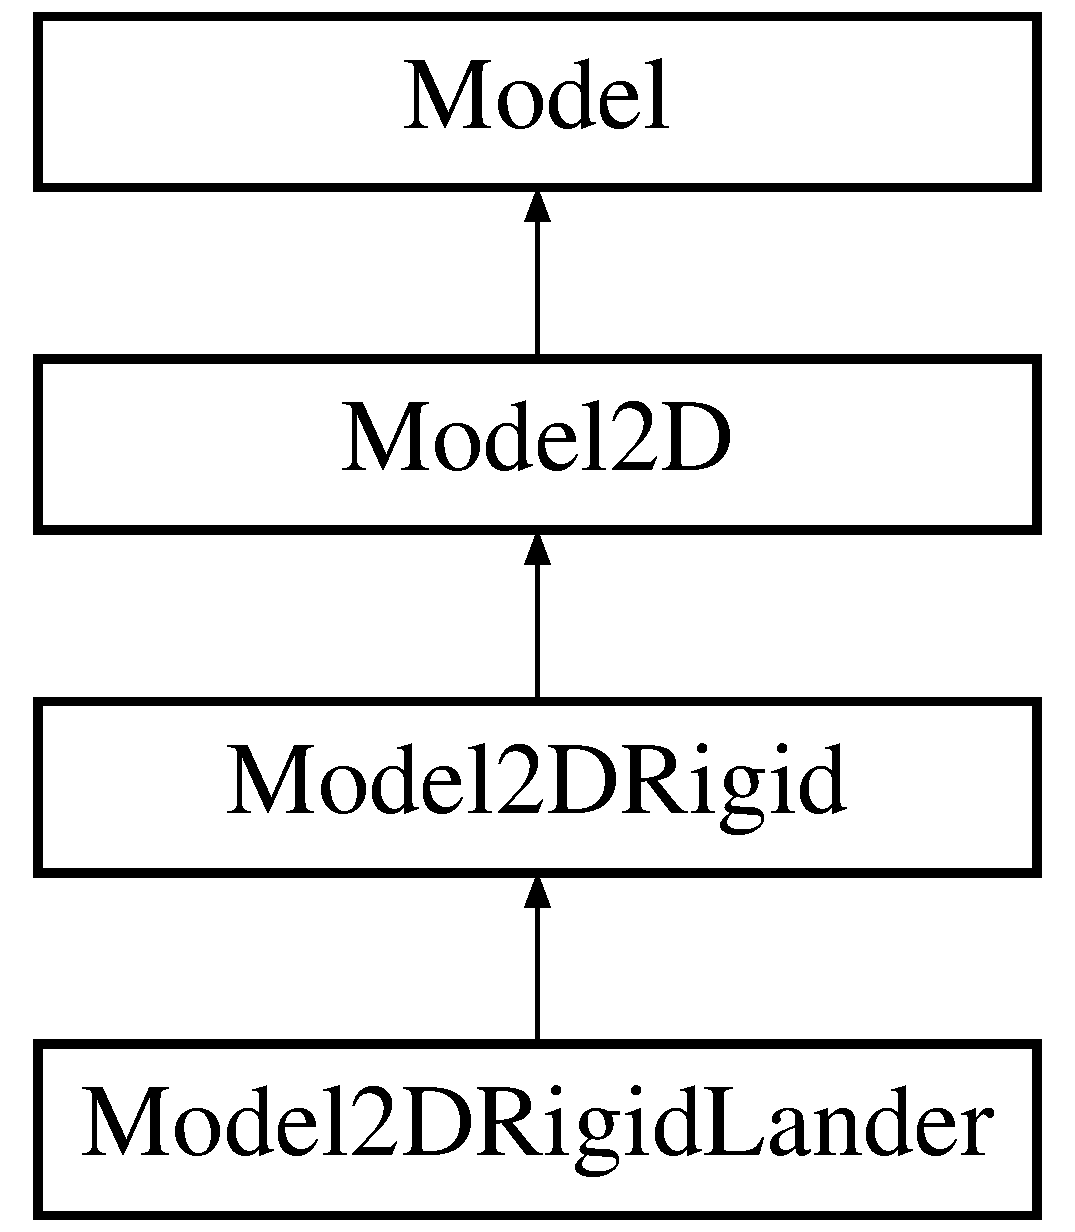
\includegraphics[height=4cm]{classModel2DRigidLander}
\end{center}
\end{figure}
\subsection*{Public Methods}
\begin{CompactItemize}
\item 
{\bf Model2DRigid\-Lander} (string path)
\item 
virtual {\bf $\sim$Model2DRigid\-Lander} ()
\item 
{\bf MSLVector} {\bf Integrate} (const {\bf MSLVector} \&x, const {\bf MSLVector} \&u, const double \&h)
\begin{CompactList}\small\item\em Perform integration from state x, using input u, over time step h.\item\end{CompactList}\item 
virtual {\bf MSLVector} {\bf State\-To\-Configuration} (const {\bf MSLVector} \&x)
\begin{CompactList}\small\item\em A method that converts a {\bf Model} {\rm (p.\,\pageref{classModel})} state in to a {\bf Geom} {\rm (p.\,\pageref{classGeom})} configuration.\item\end{CompactList}\item 
virtual {\bf MSLVector} {\bf State\-Transition\-Equation} (const {\bf MSLVector} \&x, const {\bf MSLVector} \&u)
\begin{CompactList}\small\item\em The state transition equation, or equations of motion, xdot=f(x,u).\item\end{CompactList}\item 
virtual double {\bf Metric} (const {\bf MSLVector} \&x1, const {\bf MSLVector} \&x2)
\begin{CompactList}\small\item\em A distance metric, which is Euclidean in the base class.\item\end{CompactList}\end{CompactItemize}
\subsection*{Public Attributes}
\begin{CompactItemize}
\item 
double {\bf Mass}
\begin{CompactList}\small\item\em Mass in kg.\item\end{CompactList}\item 
double {\bf G}
\begin{CompactList}\small\item\em Accel of gravity (m/s$^\wedge$2).\item\end{CompactList}\item 
double {\bf Fs}
\begin{CompactList}\small\item\em Side thruster force.\item\end{CompactList}\item 
double {\bf Fu}
\begin{CompactList}\small\item\em Upward thruster force.\item\end{CompactList}\end{CompactItemize}


\subsection{Detailed Description}
A rigid body with two small side thrusters, and a larger lower thruster. The goal is to navigate and softly \char`\"{}land\char`\"{} the craft by firing thrusters, in spite of gravity.



\subsection{Constructor \& Destructor Documentation}
\index{Model2DRigidLander@{Model2DRigid\-Lander}!Model2DRigidLander@{Model2DRigidLander}}
\index{Model2DRigidLander@{Model2DRigidLander}!Model2DRigidLander@{Model2DRigid\-Lander}}
\subsubsection{\setlength{\rightskip}{0pt plus 5cm}Model2DRigid\-Lander::Model2DRigid\-Lander (string {\em path} = \char`\"{}\char`\"{})}\label{classModel2DRigidLander_a0}


\index{Model2DRigidLander@{Model2DRigid\-Lander}!~Model2DRigidLander@{$\sim$Model2DRigidLander}}
\index{~Model2DRigidLander@{$\sim$Model2DRigidLander}!Model2DRigidLander@{Model2DRigid\-Lander}}
\subsubsection{\setlength{\rightskip}{0pt plus 5cm}Model2DRigid\-Lander::$\sim$Model2DRigid\-Lander ()\hspace{0.3cm}{\tt  [inline, virtual]}}\label{classModel2DRigidLander_a1}




\subsection{Member Function Documentation}
\index{Model2DRigidLander@{Model2DRigid\-Lander}!Integrate@{Integrate}}
\index{Integrate@{Integrate}!Model2DRigidLander@{Model2DRigid\-Lander}}
\subsubsection{\setlength{\rightskip}{0pt plus 5cm}{\bf MSLVector} Model2DRigid\-Lander::Integrate (const {\bf MSLVector} \& {\em x}, const {\bf MSLVector} \& {\em u}, const double \& {\em h})\hspace{0.3cm}{\tt  [virtual]}}\label{classModel2DRigidLander_a2}


Perform integration from state x, using input u, over time step h.



Reimplemented from {\bf Model2DRigid} {\rm (p.\,\pageref{classModel2DRigid_a2})}.\index{Model2DRigidLander@{Model2DRigid\-Lander}!Metric@{Metric}}
\index{Metric@{Metric}!Model2DRigidLander@{Model2DRigid\-Lander}}
\subsubsection{\setlength{\rightskip}{0pt plus 5cm}double Model2DRigid\-Lander::Metric (const {\bf MSLVector} \& {\em x1}, const {\bf MSLVector} \& {\em x2})\hspace{0.3cm}{\tt  [virtual]}}\label{classModel2DRigidLander_a5}


A distance metric, which is Euclidean in the base class.



Reimplemented from {\bf Model2DRigid} {\rm (p.\,\pageref{classModel2DRigid_a5})}.\index{Model2DRigidLander@{Model2DRigid\-Lander}!StateToConfiguration@{StateToConfiguration}}
\index{StateToConfiguration@{StateToConfiguration}!Model2DRigidLander@{Model2DRigid\-Lander}}
\subsubsection{\setlength{\rightskip}{0pt plus 5cm}{\bf MSLVector} Model2DRigid\-Lander::State\-To\-Configuration (const {\bf MSLVector} \& {\em x})\hspace{0.3cm}{\tt  [virtual]}}\label{classModel2DRigidLander_a3}


A method that converts a {\bf Model} {\rm (p.\,\pageref{classModel})} state in to a {\bf Geom} {\rm (p.\,\pageref{classGeom})} configuration.



Reimplemented from {\bf Model2DRigid} {\rm (p.\,\pageref{classModel2DRigid_a6})}.\index{Model2DRigidLander@{Model2DRigid\-Lander}!StateTransitionEquation@{StateTransitionEquation}}
\index{StateTransitionEquation@{StateTransitionEquation}!Model2DRigidLander@{Model2DRigid\-Lander}}
\subsubsection{\setlength{\rightskip}{0pt plus 5cm}{\bf MSLVector} Model2DRigid\-Lander::State\-Transition\-Equation (const {\bf MSLVector} \& {\em x}, const {\bf MSLVector} \& {\em u})\hspace{0.3cm}{\tt  [virtual]}}\label{classModel2DRigidLander_a4}


The state transition equation, or equations of motion, xdot=f(x,u).



Reimplemented from {\bf Model2DRigid} {\rm (p.\,\pageref{classModel2DRigid_a3})}.

\subsection{Member Data Documentation}
\index{Model2DRigidLander@{Model2DRigid\-Lander}!Fs@{Fs}}
\index{Fs@{Fs}!Model2DRigidLander@{Model2DRigid\-Lander}}
\subsubsection{\setlength{\rightskip}{0pt plus 5cm}double Model2DRigid\-Lander::Fs}\label{classModel2DRigidLander_m2}


Side thruster force.

\index{Model2DRigidLander@{Model2DRigid\-Lander}!Fu@{Fu}}
\index{Fu@{Fu}!Model2DRigidLander@{Model2DRigid\-Lander}}
\subsubsection{\setlength{\rightskip}{0pt plus 5cm}double Model2DRigid\-Lander::Fu}\label{classModel2DRigidLander_m3}


Upward thruster force.

\index{Model2DRigidLander@{Model2DRigid\-Lander}!G@{G}}
\index{G@{G}!Model2DRigidLander@{Model2DRigid\-Lander}}
\subsubsection{\setlength{\rightskip}{0pt plus 5cm}double Model2DRigid\-Lander::G}\label{classModel2DRigidLander_m1}


Accel of gravity (m/s$^\wedge$2).

\index{Model2DRigidLander@{Model2DRigid\-Lander}!Mass@{Mass}}
\index{Mass@{Mass}!Model2DRigidLander@{Model2DRigid\-Lander}}
\subsubsection{\setlength{\rightskip}{0pt plus 5cm}double Model2DRigid\-Lander::Mass}\label{classModel2DRigidLander_m0}


Mass in kg.



The documentation for this class was generated from the following files:\begin{CompactItemize}
\item 
{\bf model2d.h}\item 
{\bf model2d.C}\end{CompactItemize}

\section{Model2DRigid\-Multi  Class Reference}
\label{classModel2DRigidMulti}\index{Model2DRigidMulti@{Model2DRigid\-Multi}}
A collection of free-floating bodies in a 2D world. 


{\tt \#include $<$model2d.h$>$}

Inheritance diagram for Model2DRigid\-Multi::\begin{figure}[H]
\begin{center}
\leavevmode
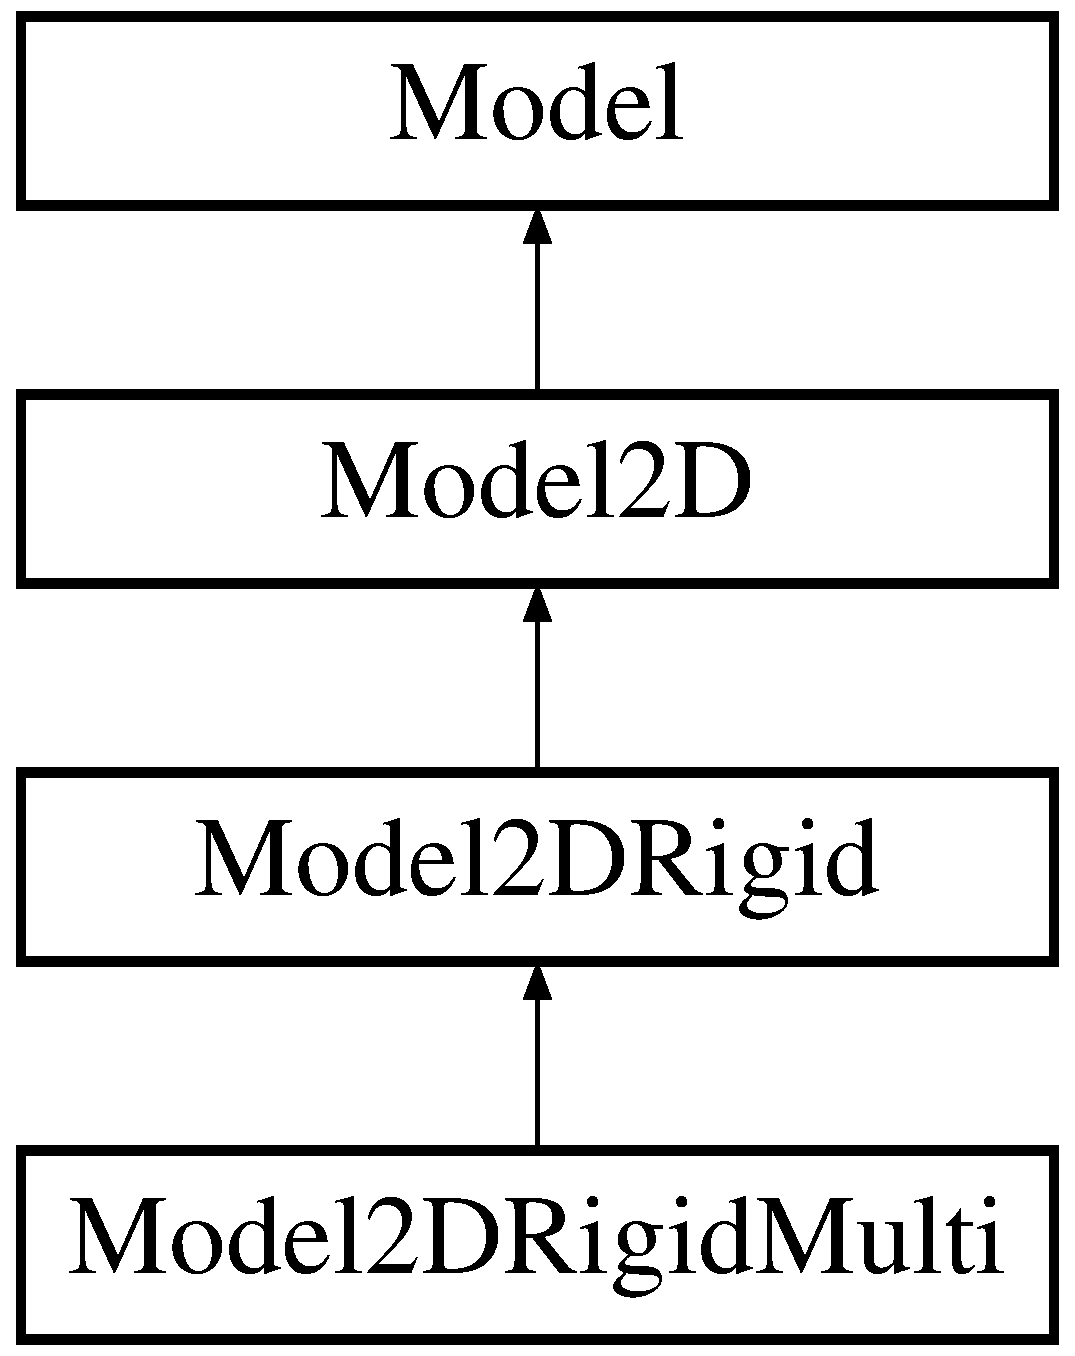
\includegraphics[height=4cm]{classModel2DRigidMulti}
\end{center}
\end{figure}
\subsection*{Public Methods}
\begin{CompactItemize}
\item 
{\bf Model2DRigid\-Multi} (string path)
\item 
virtual {\bf $\sim$Model2DRigid\-Multi} ()
\item 
virtual double {\bf Metric} (const {\bf MSLVector} \&x1, const {\bf MSLVector} \&x2)
\begin{CompactList}\small\item\em A distance metric, which is Euclidean in the base class.\item\end{CompactList}\item 
virtual {\bf MSLVector} {\bf State\-To\-Configuration} (const {\bf MSLVector} \&x)
\begin{CompactList}\small\item\em A method that converts a {\bf Model} {\rm (p.\,\pageref{classModel})} state in to a {\bf Geom} {\rm (p.\,\pageref{classGeom})} configuration.\item\end{CompactList}\item 
virtual {\bf MSLVector} {\bf Linear\-Interpolate} (const {\bf MSLVector} \&x1, const {\bf MSLVector} \&x2, const double \&a)
\begin{CompactList}\small\item\em Linearly interpolate two state while respecting topology.\item\end{CompactList}\end{CompactItemize}
\subsection*{Public Attributes}
\begin{CompactItemize}
\item 
int {\bf Num\-Bodies}
\begin{CompactList}\small\item\em Number of independent rigid bodies.\item\end{CompactList}\end{CompactItemize}


\subsection{Detailed Description}
A collection of free-floating bodies in a 2D world.



\subsection{Constructor \& Destructor Documentation}
\index{Model2DRigidMulti@{Model2DRigid\-Multi}!Model2DRigidMulti@{Model2DRigidMulti}}
\index{Model2DRigidMulti@{Model2DRigidMulti}!Model2DRigidMulti@{Model2DRigid\-Multi}}
\subsubsection{\setlength{\rightskip}{0pt plus 5cm}Model2DRigid\-Multi::Model2DRigid\-Multi (string {\em path} = \char`\"{}\char`\"{})}\label{classModel2DRigidMulti_a0}


\index{Model2DRigidMulti@{Model2DRigid\-Multi}!~Model2DRigidMulti@{$\sim$Model2DRigidMulti}}
\index{~Model2DRigidMulti@{$\sim$Model2DRigidMulti}!Model2DRigidMulti@{Model2DRigid\-Multi}}
\subsubsection{\setlength{\rightskip}{0pt plus 5cm}Model2DRigid\-Multi::$\sim$Model2DRigid\-Multi ()\hspace{0.3cm}{\tt  [inline, virtual]}}\label{classModel2DRigidMulti_a1}




\subsection{Member Function Documentation}
\index{Model2DRigidMulti@{Model2DRigid\-Multi}!LinearInterpolate@{LinearInterpolate}}
\index{LinearInterpolate@{LinearInterpolate}!Model2DRigidMulti@{Model2DRigid\-Multi}}
\subsubsection{\setlength{\rightskip}{0pt plus 5cm}{\bf MSLVector} Model2DRigid\-Multi::Linear\-Interpolate (const {\bf MSLVector} \& {\em x1}, const {\bf MSLVector} \& {\em x2}, const double \& {\em a})\hspace{0.3cm}{\tt  [virtual]}}\label{classModel2DRigidMulti_a4}


Linearly interpolate two state while respecting topology.

If a=0, then x1 is returned; if a=1, then x2 is returned. All intermediate values of \$a $\backslash$in [0,1]\$ yield intermediate states. This method is defined by {\bf Model} {\rm (p.\,\pageref{classModel})}. 

Reimplemented from {\bf Model2DRigid} {\rm (p.\,\pageref{classModel2DRigid_a4})}.\index{Model2DRigidMulti@{Model2DRigid\-Multi}!Metric@{Metric}}
\index{Metric@{Metric}!Model2DRigidMulti@{Model2DRigid\-Multi}}
\subsubsection{\setlength{\rightskip}{0pt plus 5cm}double Model2DRigid\-Multi::Metric (const {\bf MSLVector} \& {\em x1}, const {\bf MSLVector} \& {\em x2})\hspace{0.3cm}{\tt  [virtual]}}\label{classModel2DRigidMulti_a2}


A distance metric, which is Euclidean in the base class.



Reimplemented from {\bf Model2DRigid} {\rm (p.\,\pageref{classModel2DRigid_a5})}.\index{Model2DRigidMulti@{Model2DRigid\-Multi}!StateToConfiguration@{StateToConfiguration}}
\index{StateToConfiguration@{StateToConfiguration}!Model2DRigidMulti@{Model2DRigid\-Multi}}
\subsubsection{\setlength{\rightskip}{0pt plus 5cm}{\bf MSLVector} Model2DRigid\-Multi::State\-To\-Configuration (const {\bf MSLVector} \& {\em x})\hspace{0.3cm}{\tt  [virtual]}}\label{classModel2DRigidMulti_a3}


A method that converts a {\bf Model} {\rm (p.\,\pageref{classModel})} state in to a {\bf Geom} {\rm (p.\,\pageref{classGeom})} configuration.



Reimplemented from {\bf Model2DRigid} {\rm (p.\,\pageref{classModel2DRigid_a6})}.

\subsection{Member Data Documentation}
\index{Model2DRigidMulti@{Model2DRigid\-Multi}!NumBodies@{NumBodies}}
\index{NumBodies@{NumBodies}!Model2DRigidMulti@{Model2DRigid\-Multi}}
\subsubsection{\setlength{\rightskip}{0pt plus 5cm}int Model2DRigid\-Multi::Num\-Bodies}\label{classModel2DRigidMulti_m0}


Number of independent rigid bodies.



The documentation for this class was generated from the following files:\begin{CompactItemize}
\item 
{\bf model2d.h}\item 
{\bf model2d.C}\end{CompactItemize}

\section{Model3D  Class Reference}
\label{classModel3D}\index{Model3D@{Model3D}}
A base class for all models in 3D worlds. 


{\tt \#include $<$model3d.h$>$}

Inheritance diagram for Model3D::\begin{figure}[H]
\begin{center}
\leavevmode
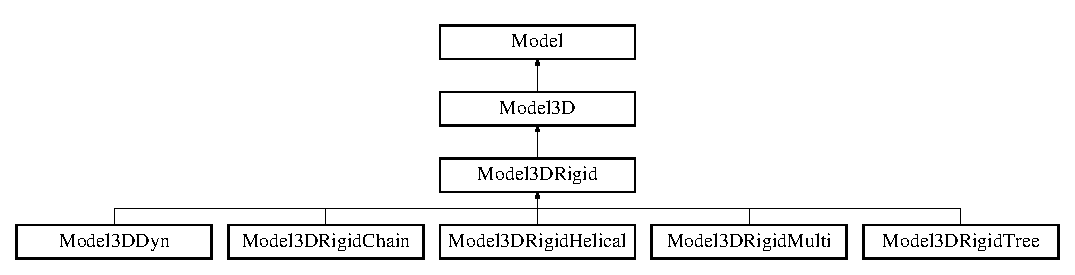
\includegraphics[height=3.24638cm]{classModel3D}
\end{center}
\end{figure}
\subsection*{Public Methods}
\begin{CompactItemize}
\item 
{\bf Model3D} (string path)
\item 
virtual {\bf $\sim$Model3D} ()
\end{CompactItemize}


\subsection{Detailed Description}
A base class for all models in 3D worlds.



\subsection{Constructor \& Destructor Documentation}
\index{Model3D@{Model3D}!Model3D@{Model3D}}
\index{Model3D@{Model3D}!Model3D@{Model3D}}
\subsubsection{\setlength{\rightskip}{0pt plus 5cm}Model3D::Model3D (string {\em path} = \char`\"{}\char`\"{})}\label{classModel3D_a0}


\index{Model3D@{Model3D}!~Model3D@{$\sim$Model3D}}
\index{~Model3D@{$\sim$Model3D}!Model3D@{Model3D}}
\subsubsection{\setlength{\rightskip}{0pt plus 5cm}Model3D::$\sim$Model3D ()\hspace{0.3cm}{\tt  [inline, virtual]}}\label{classModel3D_a1}




The documentation for this class was generated from the following files:\begin{CompactItemize}
\item 
{\bf model3d.h}\item 
{\bf model3d.C}\end{CompactItemize}

\section{Model3DDyn  Class Reference}
\label{classModel3DDyn}\index{Model3DDyn@{Model3DDyn}}
A spacecraft model with three thrusters providing both tranlation force and rotation torque. 


{\tt \#include $<$model3ddyn.h$>$}

Inheritance diagram for Model3DDyn::\begin{figure}[H]
\begin{center}
\leavevmode
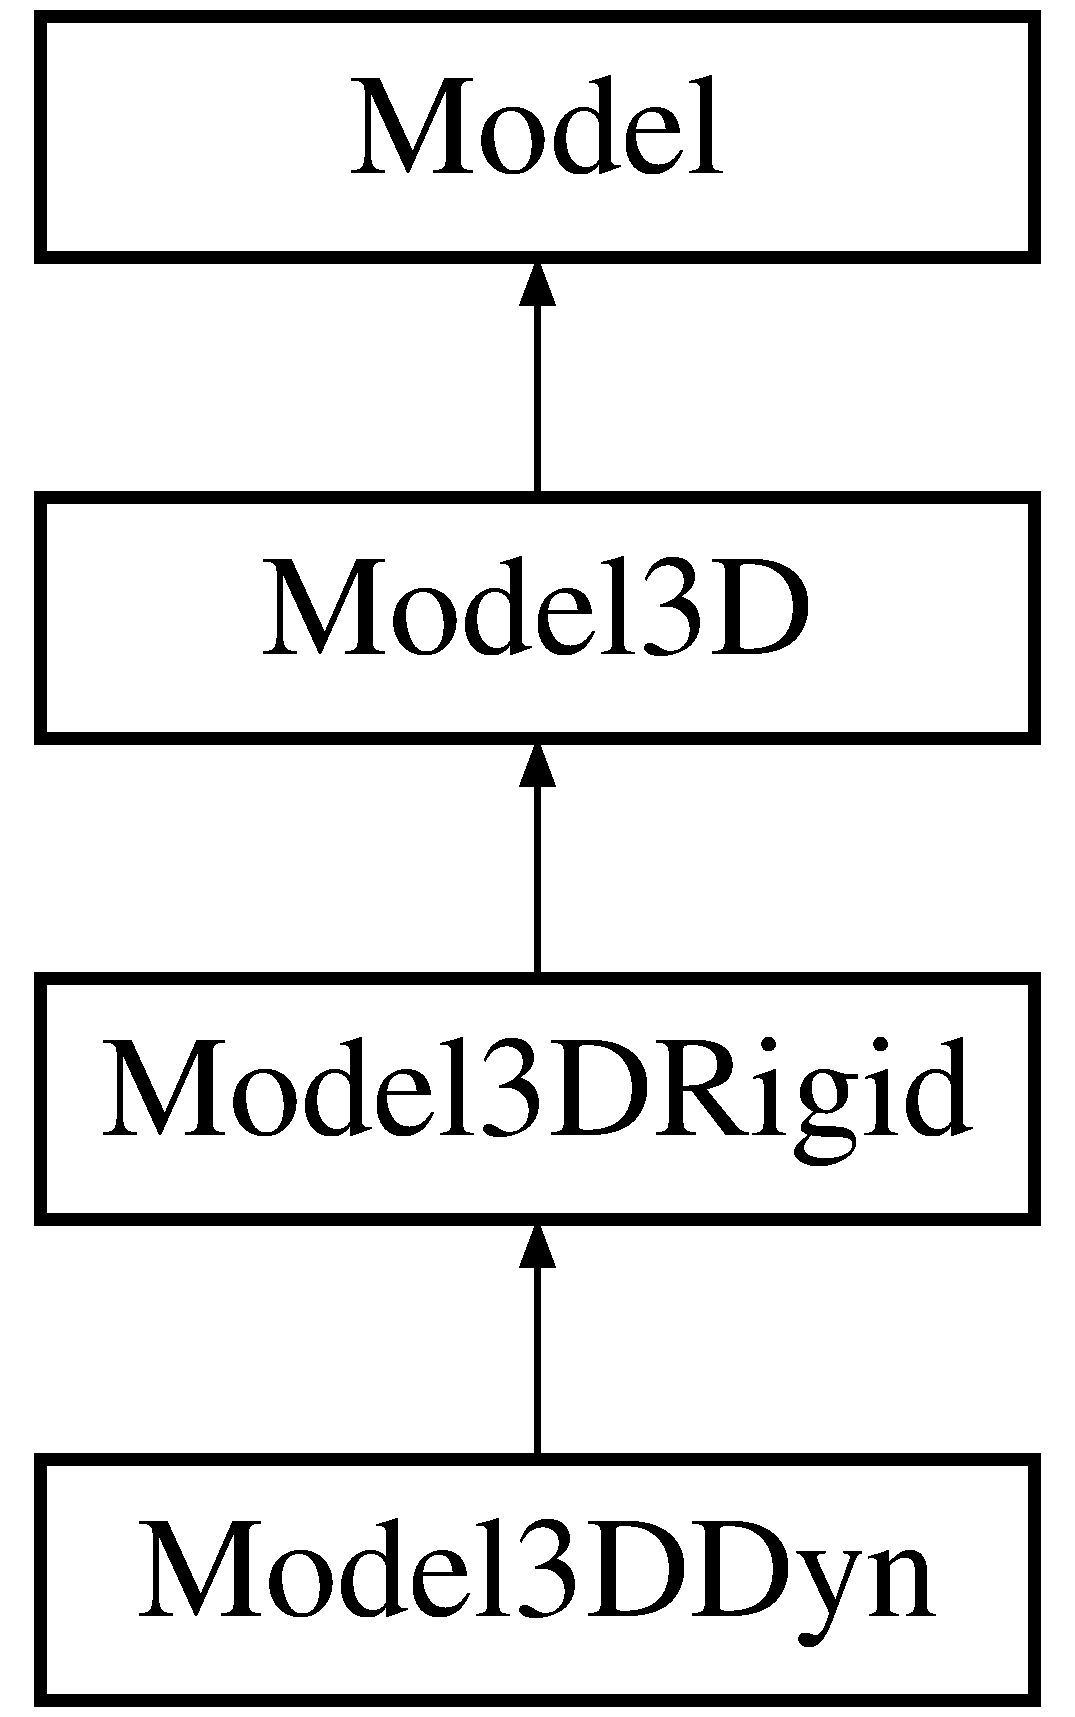
\includegraphics[height=4cm]{classModel3DDyn}
\end{center}
\end{figure}
\subsection*{Public Methods}
\begin{CompactItemize}
\item 
{\bf Model3DDyn} (string path)
\item 
virtual {\bf $\sim$Model3DDyn} ()
\item 
virtual {\bf MSLVector} {\bf State\-Transition\-Equation} (const {\bf MSLVector} \&x, const {\bf MSLVector} \&u)
\begin{CompactList}\small\item\em The state transition equation, or equations of motion, xdot=f(x,u).\item\end{CompactList}\item 
virtual bool {\bf Satisfied} (const {\bf MSLVector} \&state)
\begin{CompactList}\small\item\em Test whether global state-space constraints are satisfied.\item\end{CompactList}\end{CompactItemize}
\subsection*{Public Attributes}
\begin{CompactItemize}
\item 
double {\bf m}
\item 
{\bf MSLMatrix} {\bf I}
\end{CompactItemize}


\subsection{Detailed Description}
A spacecraft model with three thrusters providing both tranlation force and rotation torque.



\subsection{Constructor \& Destructor Documentation}
\index{Model3DDyn@{Model3DDyn}!Model3DDyn@{Model3DDyn}}
\index{Model3DDyn@{Model3DDyn}!Model3DDyn@{Model3DDyn}}
\subsubsection{\setlength{\rightskip}{0pt plus 5cm}Model3DDyn::Model3DDyn (string {\em path} = \char`\"{}\char`\"{})}\label{classModel3DDyn_a0}


\index{Model3DDyn@{Model3DDyn}!~Model3DDyn@{$\sim$Model3DDyn}}
\index{~Model3DDyn@{$\sim$Model3DDyn}!Model3DDyn@{Model3DDyn}}
\subsubsection{\setlength{\rightskip}{0pt plus 5cm}Model3DDyn::$\sim$Model3DDyn ()\hspace{0.3cm}{\tt  [inline, virtual]}}\label{classModel3DDyn_a1}




\subsection{Member Function Documentation}
\index{Model3DDyn@{Model3DDyn}!Satisfied@{Satisfied}}
\index{Satisfied@{Satisfied}!Model3DDyn@{Model3DDyn}}
\subsubsection{\setlength{\rightskip}{0pt plus 5cm}bool Model3DDyn::Satisfied (const {\bf MSLVector} \& {\em state})\hspace{0.3cm}{\tt  [virtual]}}\label{classModel3DDyn_a3}


Test whether global state-space constraints are satisfied.



Reimplemented from {\bf Model} {\rm (p.\,\pageref{classModel_a4})}.\index{Model3DDyn@{Model3DDyn}!StateTransitionEquation@{StateTransitionEquation}}
\index{StateTransitionEquation@{StateTransitionEquation}!Model3DDyn@{Model3DDyn}}
\subsubsection{\setlength{\rightskip}{0pt plus 5cm}{\bf MSLVector} Model3DDyn::State\-Transition\-Equation (const {\bf MSLVector} \& {\em x}, const {\bf MSLVector} \& {\em u})\hspace{0.3cm}{\tt  [virtual]}}\label{classModel3DDyn_a2}


The state transition equation, or equations of motion, xdot=f(x,u).



Reimplemented from {\bf Model3DRigid} {\rm (p.\,\pageref{classModel3DRigid_a3})}.

\subsection{Member Data Documentation}
\index{Model3DDyn@{Model3DDyn}!I@{I}}
\index{I@{I}!Model3DDyn@{Model3DDyn}}
\subsubsection{\setlength{\rightskip}{0pt plus 5cm}{\bf MSLMatrix} Model3DDyn::I}\label{classModel3DDyn_m1}


\index{Model3DDyn@{Model3DDyn}!m@{m}}
\index{m@{m}!Model3DDyn@{Model3DDyn}}
\subsubsection{\setlength{\rightskip}{0pt plus 5cm}double Model3DDyn::m}\label{classModel3DDyn_m0}




The documentation for this class was generated from the following files:\begin{CompactItemize}
\item 
{\bf model3ddyn.h}\item 
{\bf model3ddyn.C}\end{CompactItemize}

\section{Model3DRigid  Class Reference}
\label{classModel3DRigid}\index{Model3DRigid@{Model3DRigid}}
A rigid robot in a 3D world. 


{\tt \#include $<$model3d.h$>$}

Inheritance diagram for Model3DRigid::\begin{figure}[H]
\begin{center}
\leavevmode
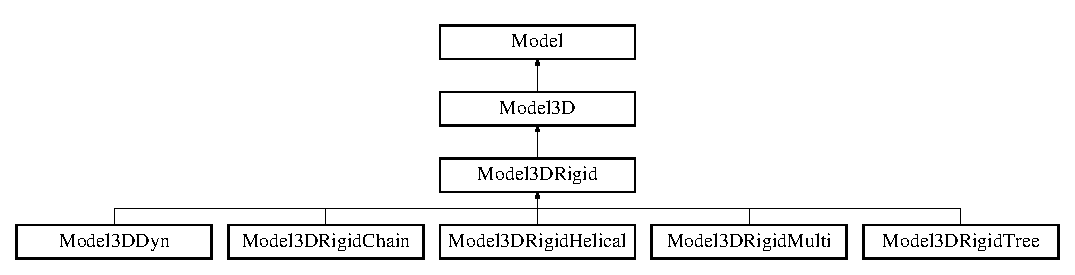
\includegraphics[height=3.24638cm]{classModel3DRigid}
\end{center}
\end{figure}
\subsection*{Public Methods}
\begin{CompactItemize}
\item 
{\bf Model3DRigid} (string path)
\item 
virtual {\bf $\sim$Model3DRigid} ()
\item 
virtual {\bf MSLVector} {\bf Integrate} (const {\bf MSLVector} \&x, const {\bf MSLVector} \&u, const double \&h)
\begin{CompactList}\small\item\em Perform integration from state x, using input u, over time step h.\item\end{CompactList}\item 
{\bf MSLVector} {\bf State\-Transition\-Equation} (const {\bf MSLVector} \&x, const {\bf MSLVector} \&u)
\begin{CompactList}\small\item\em The state transition equation, or equations of motion, xdot=f(x,u).\item\end{CompactList}\item 
virtual double {\bf Metric} (const {\bf MSLVector} \&x1, const {\bf MSLVector} \&x2)
\begin{CompactList}\small\item\em A distance metric, which is Euclidean in the base class.\item\end{CompactList}\item 
virtual {\bf MSLVector} {\bf Linear\-Interpolate} (const {\bf MSLVector} \&x1, const {\bf MSLVector} \&x2, const double \&a)
\begin{CompactList}\small\item\em Linearly interpolate two state while respecting topology.\item\end{CompactList}\end{CompactItemize}


\subsection{Detailed Description}
A rigid robot in a 3D world.



\subsection{Constructor \& Destructor Documentation}
\index{Model3DRigid@{Model3DRigid}!Model3DRigid@{Model3DRigid}}
\index{Model3DRigid@{Model3DRigid}!Model3DRigid@{Model3DRigid}}
\subsubsection{\setlength{\rightskip}{0pt plus 5cm}Model3DRigid::Model3DRigid (string {\em path} = \char`\"{}\char`\"{})}\label{classModel3DRigid_a0}


\index{Model3DRigid@{Model3DRigid}!~Model3DRigid@{$\sim$Model3DRigid}}
\index{~Model3DRigid@{$\sim$Model3DRigid}!Model3DRigid@{Model3DRigid}}
\subsubsection{\setlength{\rightskip}{0pt plus 5cm}Model3DRigid::$\sim$Model3DRigid ()\hspace{0.3cm}{\tt  [inline, virtual]}}\label{classModel3DRigid_a1}




\subsection{Member Function Documentation}
\index{Model3DRigid@{Model3DRigid}!Integrate@{Integrate}}
\index{Integrate@{Integrate}!Model3DRigid@{Model3DRigid}}
\subsubsection{\setlength{\rightskip}{0pt plus 5cm}{\bf MSLVector} Model3DRigid::Integrate (const {\bf MSLVector} \& {\em x}, const {\bf MSLVector} \& {\em u}, const double \& {\em h})\hspace{0.3cm}{\tt  [virtual]}}\label{classModel3DRigid_a2}


Perform integration from state x, using input u, over time step h.



Reimplemented from {\bf Model} {\rm (p.\,\pageref{classModel_a5})}.

Reimplemented in {\bf Model3DRigid\-Helical} {\rm (p.\,\pageref{classModel3DRigidHelical_a3})}.\index{Model3DRigid@{Model3DRigid}!LinearInterpolate@{LinearInterpolate}}
\index{LinearInterpolate@{LinearInterpolate}!Model3DRigid@{Model3DRigid}}
\subsubsection{\setlength{\rightskip}{0pt plus 5cm}{\bf MSLVector} Model3DRigid::Linear\-Interpolate (const {\bf MSLVector} \& {\em x1}, const {\bf MSLVector} \& {\em x2}, const double \& {\em a})\hspace{0.3cm}{\tt  [virtual]}}\label{classModel3DRigid_a5}


Linearly interpolate two state while respecting topology.

If a=0, then x1 is returned; if a=1, then x2 is returned. All intermediate values of \$a $\backslash$in [0,1]\$ yield intermediate states. This method is defined by {\bf Model} {\rm (p.\,\pageref{classModel})}. 

Reimplemented from {\bf Model} {\rm (p.\,\pageref{classModel_a6})}.

Reimplemented in {\bf Model3DRigid\-Multi} {\rm (p.\,\pageref{classModel3DRigidMulti_a3})}, {\bf Model3DRigid\-Chain} {\rm (p.\,\pageref{classModel3DRigidChain_a4})}, and {\bf Model3DRigid\-Tree} {\rm (p.\,\pageref{classModel3DRigidTree_a4})}.\index{Model3DRigid@{Model3DRigid}!Metric@{Metric}}
\index{Metric@{Metric}!Model3DRigid@{Model3DRigid}}
\subsubsection{\setlength{\rightskip}{0pt plus 5cm}double Model3DRigid::Metric (const {\bf MSLVector} \& {\em x1}, const {\bf MSLVector} \& {\em x2})\hspace{0.3cm}{\tt  [virtual]}}\label{classModel3DRigid_a4}


A distance metric, which is Euclidean in the base class.



Reimplemented from {\bf Model} {\rm (p.\,\pageref{classModel_a9})}.

Reimplemented in {\bf Model3DRigid\-Multi} {\rm (p.\,\pageref{classModel3DRigidMulti_a2})}, {\bf Model3DRigid\-Chain} {\rm (p.\,\pageref{classModel3DRigidChain_a5})}, and {\bf Model3DRigid\-Tree} {\rm (p.\,\pageref{classModel3DRigidTree_a5})}.\index{Model3DRigid@{Model3DRigid}!StateTransitionEquation@{StateTransitionEquation}}
\index{StateTransitionEquation@{StateTransitionEquation}!Model3DRigid@{Model3DRigid}}
\subsubsection{\setlength{\rightskip}{0pt plus 5cm}{\bf MSLVector} Model3DRigid::State\-Transition\-Equation (const {\bf MSLVector} \& {\em x}, const {\bf MSLVector} \& {\em u})\hspace{0.3cm}{\tt  [virtual]}}\label{classModel3DRigid_a3}


The state transition equation, or equations of motion, xdot=f(x,u).



Reimplemented from {\bf Model} {\rm (p.\,\pageref{classModel_a3})}.

Reimplemented in {\bf Model3DRigid\-Chain} {\rm (p.\,\pageref{classModel3DRigidChain_a2})}, {\bf Model3DRigid\-Tree} {\rm (p.\,\pageref{classModel3DRigidTree_a2})}, {\bf Model3DDyn} {\rm (p.\,\pageref{classModel3DDyn_a2})}, and {\bf Model3DRigid\-Helical} {\rm (p.\,\pageref{classModel3DRigidHelical_a2})}.

The documentation for this class was generated from the following files:\begin{CompactItemize}
\item 
{\bf model3d.h}\item 
{\bf model3d.C}\end{CompactItemize}

\section{Model3DRigid\-Chain  Class Reference}
\label{classModel3DRigidChain}\index{Model3DRigidChain@{Model3DRigid\-Chain}}
A 3D kinematic chain of bodies that uses DH parameters. 


{\tt \#include $<$model3d.h$>$}

Inheritance diagram for Model3DRigid\-Chain::\begin{figure}[H]
\begin{center}
\leavevmode
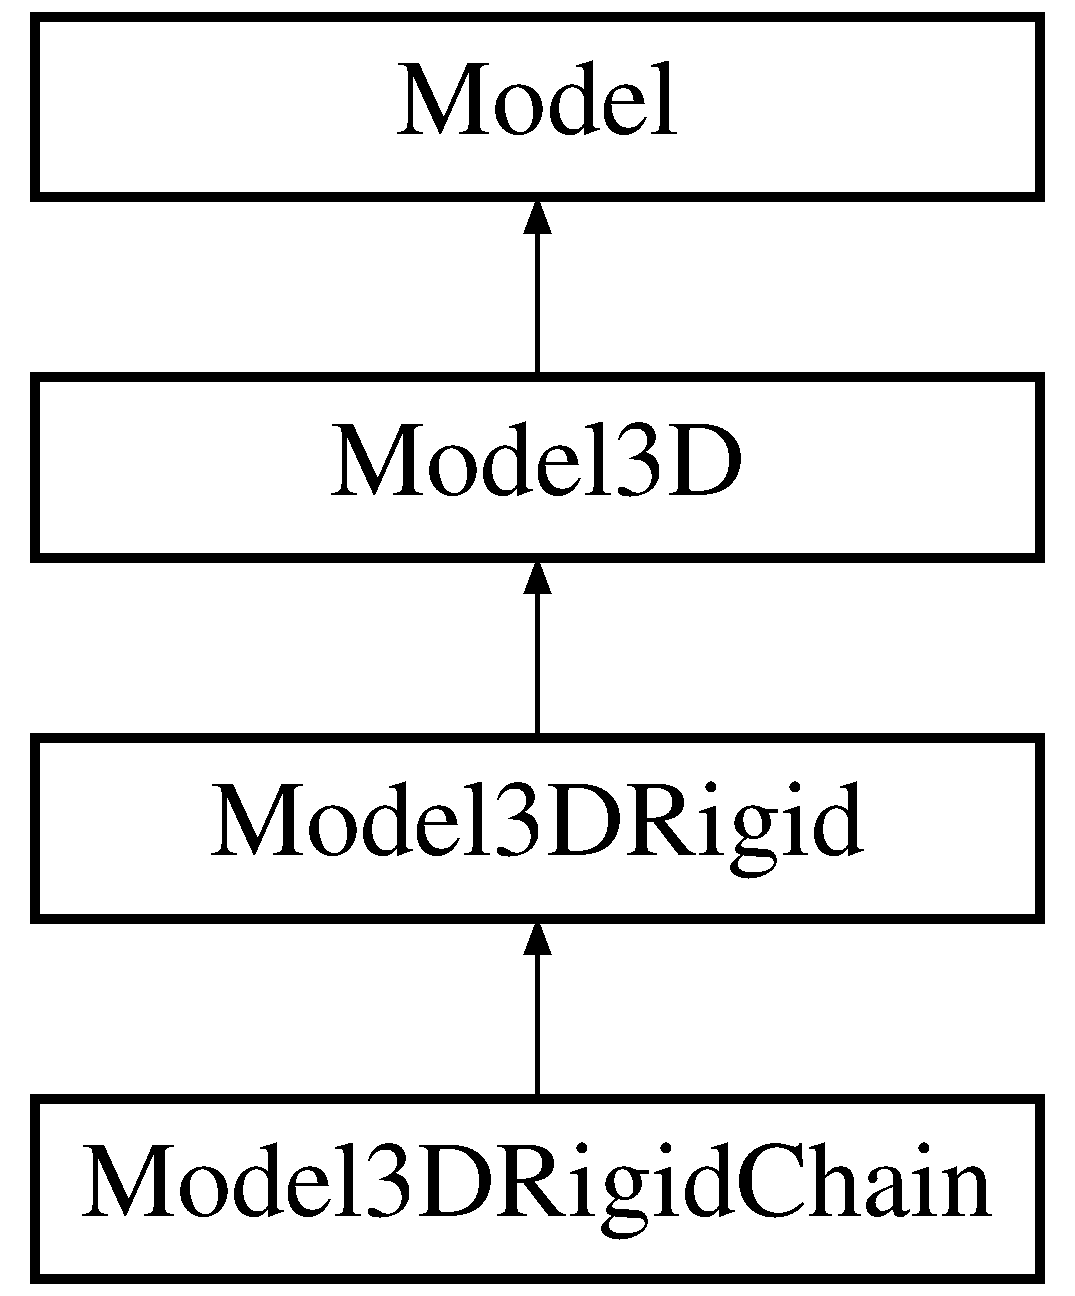
\includegraphics[height=4cm]{classModel3DRigidChain}
\end{center}
\end{figure}
\subsection*{Public Methods}
\begin{CompactItemize}
\item 
{\bf Model3DRigid\-Chain} (string path)
\item 
virtual {\bf $\sim$Model3DRigid\-Chain} ()
\item 
virtual {\bf MSLVector} {\bf State\-Transition\-Equation} (const {\bf MSLVector} \&x, const {\bf MSLVector} \&u)
\begin{CompactList}\small\item\em The state transition equation, or equations of motion, xdot=f(x,u).\item\end{CompactList}\item 
virtual {\bf MSLVector} {\bf State\-To\-Configuration} (const {\bf MSLVector} \&x)
\begin{CompactList}\small\item\em A method that converts a {\bf Model} {\rm (p.\,\pageref{classModel})} state in to a {\bf Geom} {\rm (p.\,\pageref{classGeom})} configuration.\item\end{CompactList}\item 
virtual {\bf MSLVector} {\bf Linear\-Interpolate} (const {\bf MSLVector} \&x1, const {\bf MSLVector} \&x2, const double \&a)
\begin{CompactList}\small\item\em Linearly interpolate two state while respecting topology.\item\end{CompactList}\item 
virtual double {\bf Metric} (const {\bf MSLVector} \&x1, const {\bf MSLVector} \&x2)
\begin{CompactList}\small\item\em A distance metric, which is Euclidean in the base class.\item\end{CompactList}\item 
virtual bool {\bf Satisfied} (const {\bf MSLVector} \&x)
\begin{CompactList}\small\item\em Test whether global state-space constraints are satisfied.\item\end{CompactList}\end{CompactItemize}
\subsection*{Public Attributes}
\begin{CompactItemize}
\item 
int {\bf Num\-Bodies}
\begin{CompactList}\small\item\em Number of bodies in the chain.\item\end{CompactList}\item 
{\bf MSLVector} {\bf DH}
\begin{CompactList}\small\item\em The distances between joints (\char`\"{}a\char`\"{} parameters in kinematics).\item\end{CompactList}\item 
vector$<$int$>$ {\bf State\-Indices}
\end{CompactItemize}


\subsection{Detailed Description}
A 3D kinematic chain of bodies that uses DH parameters.

A 3D kinematic chain of bodies that uses DH parameters that should be given in a DH file in the following order: Alpha(1,2...), Theta(1,2...), A(1,2...), D(1,2...). Some of these parameters change during the movement, and each of these parameters becomes a state variable. The indices of these parameters should be given in the file State\-Indices (i.e., each entry corresponds to a state, and indicates which DH parameter is variable). 



\subsection{Constructor \& Destructor Documentation}
\index{Model3DRigidChain@{Model3DRigid\-Chain}!Model3DRigidChain@{Model3DRigidChain}}
\index{Model3DRigidChain@{Model3DRigidChain}!Model3DRigidChain@{Model3DRigid\-Chain}}
\subsubsection{\setlength{\rightskip}{0pt plus 5cm}Model3DRigid\-Chain::Model3DRigid\-Chain (string {\em path} = \char`\"{}\char`\"{})}\label{classModel3DRigidChain_a0}


\index{Model3DRigidChain@{Model3DRigid\-Chain}!~Model3DRigidChain@{$\sim$Model3DRigidChain}}
\index{~Model3DRigidChain@{$\sim$Model3DRigidChain}!Model3DRigidChain@{Model3DRigid\-Chain}}
\subsubsection{\setlength{\rightskip}{0pt plus 5cm}Model3DRigid\-Chain::$\sim$Model3DRigid\-Chain ()\hspace{0.3cm}{\tt  [inline, virtual]}}\label{classModel3DRigidChain_a1}




\subsection{Member Function Documentation}
\index{Model3DRigidChain@{Model3DRigid\-Chain}!LinearInterpolate@{LinearInterpolate}}
\index{LinearInterpolate@{LinearInterpolate}!Model3DRigidChain@{Model3DRigid\-Chain}}
\subsubsection{\setlength{\rightskip}{0pt plus 5cm}{\bf MSLVector} Model3DRigid\-Chain::Linear\-Interpolate (const {\bf MSLVector} \& {\em x1}, const {\bf MSLVector} \& {\em x2}, const double \& {\em a})\hspace{0.3cm}{\tt  [virtual]}}\label{classModel3DRigidChain_a4}


Linearly interpolate two state while respecting topology.

If a=0, then x1 is returned; if a=1, then x2 is returned. All intermediate values of \$a $\backslash$in [0,1]\$ yield intermediate states. This method is defined by {\bf Model} {\rm (p.\,\pageref{classModel})}. 

Reimplemented from {\bf Model3DRigid} {\rm (p.\,\pageref{classModel3DRigid_a5})}.\index{Model3DRigidChain@{Model3DRigid\-Chain}!Metric@{Metric}}
\index{Metric@{Metric}!Model3DRigidChain@{Model3DRigid\-Chain}}
\subsubsection{\setlength{\rightskip}{0pt plus 5cm}double Model3DRigid\-Chain::Metric (const {\bf MSLVector} \& {\em x1}, const {\bf MSLVector} \& {\em x2})\hspace{0.3cm}{\tt  [virtual]}}\label{classModel3DRigidChain_a5}


A distance metric, which is Euclidean in the base class.



Reimplemented from {\bf Model3DRigid} {\rm (p.\,\pageref{classModel3DRigid_a4})}.\index{Model3DRigidChain@{Model3DRigid\-Chain}!Satisfied@{Satisfied}}
\index{Satisfied@{Satisfied}!Model3DRigidChain@{Model3DRigid\-Chain}}
\subsubsection{\setlength{\rightskip}{0pt plus 5cm}bool Model3DRigid\-Chain::Satisfied (const {\bf MSLVector} \& {\em x})\hspace{0.3cm}{\tt  [virtual]}}\label{classModel3DRigidChain_a6}


Test whether global state-space constraints are satisfied.



Reimplemented from {\bf Model} {\rm (p.\,\pageref{classModel_a4})}.\index{Model3DRigidChain@{Model3DRigid\-Chain}!StateToConfiguration@{StateToConfiguration}}
\index{StateToConfiguration@{StateToConfiguration}!Model3DRigidChain@{Model3DRigid\-Chain}}
\subsubsection{\setlength{\rightskip}{0pt plus 5cm}{\bf MSLVector} Model3DRigid\-Chain::State\-To\-Configuration (const {\bf MSLVector} \& {\em x})\hspace{0.3cm}{\tt  [virtual]}}\label{classModel3DRigidChain_a3}


A method that converts a {\bf Model} {\rm (p.\,\pageref{classModel})} state in to a {\bf Geom} {\rm (p.\,\pageref{classGeom})} configuration.



Reimplemented from {\bf Model} {\rm (p.\,\pageref{classModel_a8})}.\index{Model3DRigidChain@{Model3DRigid\-Chain}!StateTransitionEquation@{StateTransitionEquation}}
\index{StateTransitionEquation@{StateTransitionEquation}!Model3DRigidChain@{Model3DRigid\-Chain}}
\subsubsection{\setlength{\rightskip}{0pt plus 5cm}{\bf MSLVector} Model3DRigid\-Chain::State\-Transition\-Equation (const {\bf MSLVector} \& {\em x}, const {\bf MSLVector} \& {\em u})\hspace{0.3cm}{\tt  [virtual]}}\label{classModel3DRigidChain_a2}


The state transition equation, or equations of motion, xdot=f(x,u).



Reimplemented from {\bf Model3DRigid} {\rm (p.\,\pageref{classModel3DRigid_a3})}.

\subsection{Member Data Documentation}
\index{Model3DRigidChain@{Model3DRigid\-Chain}!DH@{DH}}
\index{DH@{DH}!Model3DRigidChain@{Model3DRigid\-Chain}}
\subsubsection{\setlength{\rightskip}{0pt plus 5cm}{\bf MSLVector} Model3DRigid\-Chain::DH}\label{classModel3DRigidChain_m1}


The distances between joints (\char`\"{}a\char`\"{} parameters in kinematics).

\index{Model3DRigidChain@{Model3DRigid\-Chain}!NumBodies@{NumBodies}}
\index{NumBodies@{NumBodies}!Model3DRigidChain@{Model3DRigid\-Chain}}
\subsubsection{\setlength{\rightskip}{0pt plus 5cm}int Model3DRigid\-Chain::Num\-Bodies}\label{classModel3DRigidChain_m0}


Number of bodies in the chain.

\index{Model3DRigidChain@{Model3DRigid\-Chain}!StateIndices@{StateIndices}}
\index{StateIndices@{StateIndices}!Model3DRigidChain@{Model3DRigid\-Chain}}
\subsubsection{\setlength{\rightskip}{0pt plus 5cm}vector$<$ int $>$ Model3DRigid\-Chain::State\-Indices$<$int$>$}\label{classModel3DRigidChain_m2}




The documentation for this class was generated from the following files:\begin{CompactItemize}
\item 
{\bf model3d.h}\item 
{\bf model3d.C}\end{CompactItemize}

\section{Model3DRigid\-Helical  Class Reference}
\label{classModel3DRigidHelical}\index{Model3DRigidHelical@{Model3DRigid\-Helical}}
A rigid robot that moves along helical paths in a 3D world. 


{\tt \#include $<$modelnew.h$>$}

Inheritance diagram for Model3DRigid\-Helical::\begin{figure}[H]
\begin{center}
\leavevmode
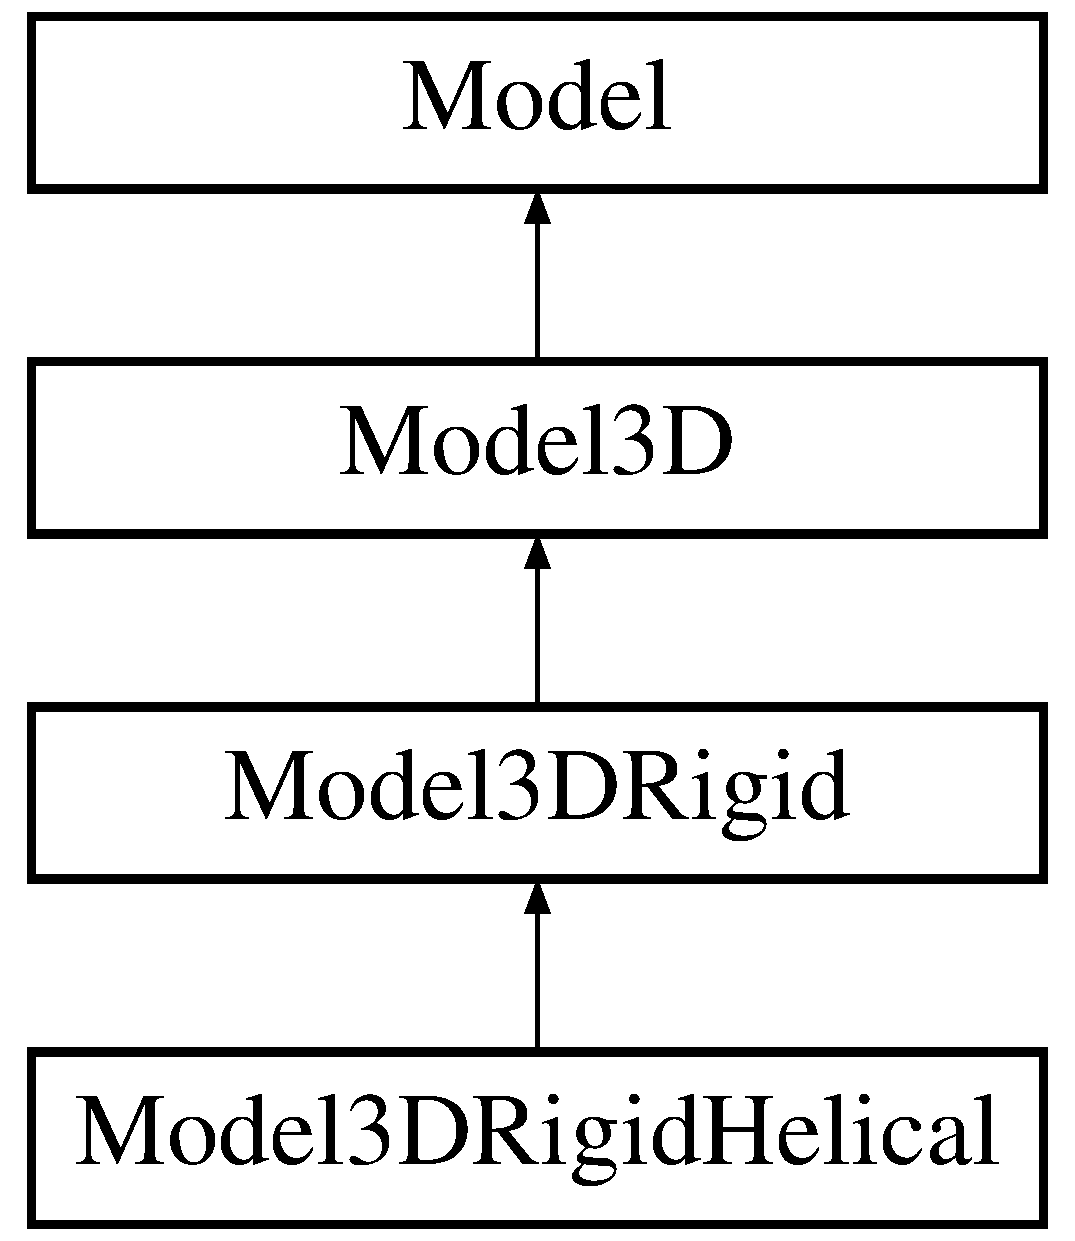
\includegraphics[height=4cm]{classModel3DRigidHelical}
\end{center}
\end{figure}
\subsection*{Public Methods}
\begin{CompactItemize}
\item 
{\bf Model3DRigid\-Helical} (string path)
\item 
virtual {\bf $\sim$Model3DRigid\-Helical} ()
\item 
virtual {\bf MSLVector} {\bf State\-Transition\-Equation} (const {\bf MSLVector} \&x, const {\bf MSLVector} \&u)
\begin{CompactList}\small\item\em Give the equations of motion for a helical kinematic system.\item\end{CompactList}\item 
virtual {\bf MSLVector} {\bf Integrate} (const {\bf MSLVector} \&x, const {\bf MSLVector} \&u, const double \&h)
\begin{CompactList}\small\item\em Perform integration from state x, using input u, over time step h.\item\end{CompactList}\end{CompactItemize}


\subsection{Detailed Description}
A rigid robot that moves along helical paths in a 3D world.



\subsection{Constructor \& Destructor Documentation}
\index{Model3DRigidHelical@{Model3DRigid\-Helical}!Model3DRigidHelical@{Model3DRigidHelical}}
\index{Model3DRigidHelical@{Model3DRigidHelical}!Model3DRigidHelical@{Model3DRigid\-Helical}}
\subsubsection{\setlength{\rightskip}{0pt plus 5cm}Model3DRigid\-Helical::Model3DRigid\-Helical (string {\em path} = \char`\"{}\char`\"{})}\label{classModel3DRigidHelical_a0}


\index{Model3DRigidHelical@{Model3DRigid\-Helical}!~Model3DRigidHelical@{$\sim$Model3DRigidHelical}}
\index{~Model3DRigidHelical@{$\sim$Model3DRigidHelical}!Model3DRigidHelical@{Model3DRigid\-Helical}}
\subsubsection{\setlength{\rightskip}{0pt plus 5cm}Model3DRigid\-Helical::$\sim$Model3DRigid\-Helical ()\hspace{0.3cm}{\tt  [inline, virtual]}}\label{classModel3DRigidHelical_a1}




\subsection{Member Function Documentation}
\index{Model3DRigidHelical@{Model3DRigid\-Helical}!Integrate@{Integrate}}
\index{Integrate@{Integrate}!Model3DRigidHelical@{Model3DRigid\-Helical}}
\subsubsection{\setlength{\rightskip}{0pt plus 5cm}{\bf MSLVector} Model3DRigid\-Helical::Integrate (const {\bf MSLVector} \& {\em x}, const {\bf MSLVector} \& {\em u}, const double \& {\em h})\hspace{0.3cm}{\tt  [virtual]}}\label{classModel3DRigidHelical_a3}


Perform integration from state x, using input u, over time step h.



Reimplemented from {\bf Model3DRigid} {\rm (p.\,\pageref{classModel3DRigid_a2})}.\index{Model3DRigidHelical@{Model3DRigid\-Helical}!StateTransitionEquation@{StateTransitionEquation}}
\index{StateTransitionEquation@{StateTransitionEquation}!Model3DRigidHelical@{Model3DRigid\-Helical}}
\subsubsection{\setlength{\rightskip}{0pt plus 5cm}{\bf MSLVector} Model3DRigid\-Helical::State\-Transition\-Equation (const {\bf MSLVector} \& {\em x}, const {\bf MSLVector} \& {\em u})\hspace{0.3cm}{\tt  [virtual]}}\label{classModel3DRigidHelical_a2}


Give the equations of motion for a helical kinematic system.



Reimplemented from {\bf Model3DRigid} {\rm (p.\,\pageref{classModel3DRigid_a3})}.

The documentation for this class was generated from the following files:\begin{CompactItemize}
\item 
{\bf modelnew.h}\item 
{\bf modelnew.C}\end{CompactItemize}

\section{Model3DRigid\-Multi  Class Reference}
\label{classModel3DRigidMulti}\index{Model3DRigidMulti@{Model3DRigid\-Multi}}
A collection of free-floating bodies in a 3D world. 


{\tt \#include $<$model3d.h$>$}

Inheritance diagram for Model3DRigid\-Multi::\begin{figure}[H]
\begin{center}
\leavevmode
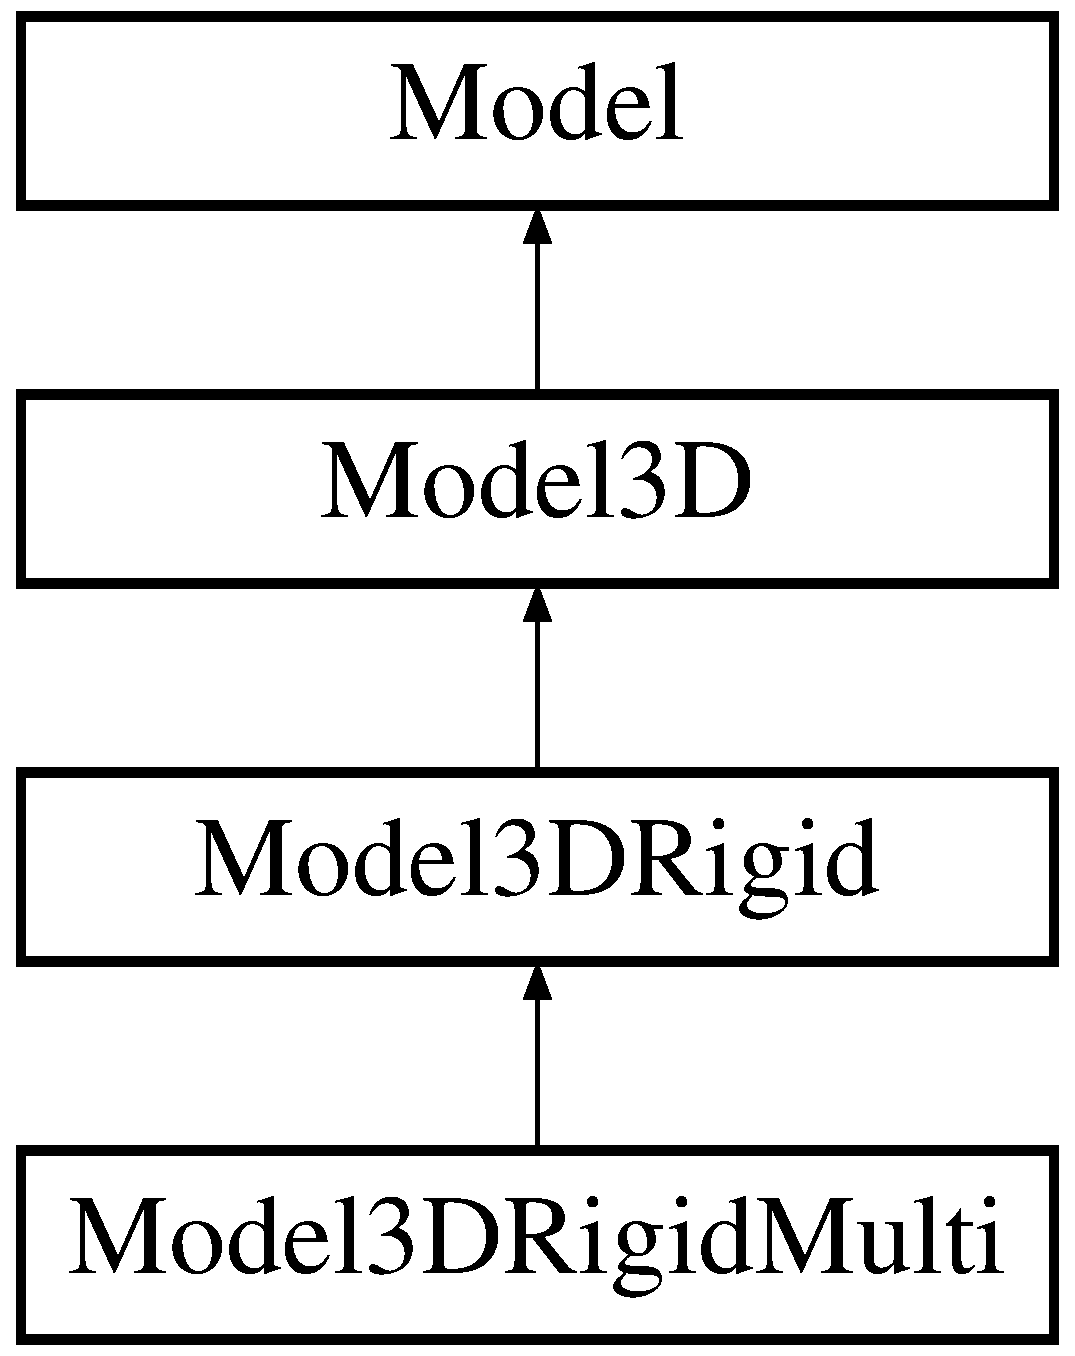
\includegraphics[height=4cm]{classModel3DRigidMulti}
\end{center}
\end{figure}
\subsection*{Public Methods}
\begin{CompactItemize}
\item 
{\bf Model3DRigid\-Multi} (string path)
\item 
virtual {\bf $\sim$Model3DRigid\-Multi} ()
\item 
virtual double {\bf Metric} (const {\bf MSLVector} \&x1, const {\bf MSLVector} \&x2)
\begin{CompactList}\small\item\em A distance metric, which is Euclidean in the base class.\item\end{CompactList}\item 
virtual {\bf MSLVector} {\bf Linear\-Interpolate} (const {\bf MSLVector} \&x1, const {\bf MSLVector} \&x2, const double \&a)
\begin{CompactList}\small\item\em Linearly interpolate two state while respecting topology.\item\end{CompactList}\end{CompactItemize}
\subsection*{Public Attributes}
\begin{CompactItemize}
\item 
int {\bf Num\-Bodies}
\end{CompactItemize}


\subsection{Detailed Description}
A collection of free-floating bodies in a 3D world.



\subsection{Constructor \& Destructor Documentation}
\index{Model3DRigidMulti@{Model3DRigid\-Multi}!Model3DRigidMulti@{Model3DRigidMulti}}
\index{Model3DRigidMulti@{Model3DRigidMulti}!Model3DRigidMulti@{Model3DRigid\-Multi}}
\subsubsection{\setlength{\rightskip}{0pt plus 5cm}Model3DRigid\-Multi::Model3DRigid\-Multi (string {\em path} = \char`\"{}\char`\"{})}\label{classModel3DRigidMulti_a0}


\index{Model3DRigidMulti@{Model3DRigid\-Multi}!~Model3DRigidMulti@{$\sim$Model3DRigidMulti}}
\index{~Model3DRigidMulti@{$\sim$Model3DRigidMulti}!Model3DRigidMulti@{Model3DRigid\-Multi}}
\subsubsection{\setlength{\rightskip}{0pt plus 5cm}Model3DRigid\-Multi::$\sim$Model3DRigid\-Multi ()\hspace{0.3cm}{\tt  [inline, virtual]}}\label{classModel3DRigidMulti_a1}




\subsection{Member Function Documentation}
\index{Model3DRigidMulti@{Model3DRigid\-Multi}!LinearInterpolate@{LinearInterpolate}}
\index{LinearInterpolate@{LinearInterpolate}!Model3DRigidMulti@{Model3DRigid\-Multi}}
\subsubsection{\setlength{\rightskip}{0pt plus 5cm}{\bf MSLVector} Model3DRigid\-Multi::Linear\-Interpolate (const {\bf MSLVector} \& {\em x1}, const {\bf MSLVector} \& {\em x2}, const double \& {\em a})\hspace{0.3cm}{\tt  [virtual]}}\label{classModel3DRigidMulti_a3}


Linearly interpolate two state while respecting topology.

If a=0, then x1 is returned; if a=1, then x2 is returned. All intermediate values of \$a $\backslash$in [0,1]\$ yield intermediate states. This method is defined by {\bf Model} {\rm (p.\,\pageref{classModel})}. 

Reimplemented from {\bf Model3DRigid} {\rm (p.\,\pageref{classModel3DRigid_a5})}.\index{Model3DRigidMulti@{Model3DRigid\-Multi}!Metric@{Metric}}
\index{Metric@{Metric}!Model3DRigidMulti@{Model3DRigid\-Multi}}
\subsubsection{\setlength{\rightskip}{0pt plus 5cm}double Model3DRigid\-Multi::Metric (const {\bf MSLVector} \& {\em x1}, const {\bf MSLVector} \& {\em x2})\hspace{0.3cm}{\tt  [virtual]}}\label{classModel3DRigidMulti_a2}


A distance metric, which is Euclidean in the base class.



Reimplemented from {\bf Model3DRigid} {\rm (p.\,\pageref{classModel3DRigid_a4})}.

\subsection{Member Data Documentation}
\index{Model3DRigidMulti@{Model3DRigid\-Multi}!NumBodies@{NumBodies}}
\index{NumBodies@{NumBodies}!Model3DRigidMulti@{Model3DRigid\-Multi}}
\subsubsection{\setlength{\rightskip}{0pt plus 5cm}int Model3DRigid\-Multi::Num\-Bodies}\label{classModel3DRigidMulti_m0}




The documentation for this class was generated from the following files:\begin{CompactItemize}
\item 
{\bf model3d.h}\item 
{\bf model3d.C}\end{CompactItemize}

\section{Model3DRigid\-Tree  Class Reference}
\label{classModel3DRigidTree}\index{Model3DRigidTree@{Model3DRigid\-Tree}}
A 3D kinematic tree of bodies that uses DH parameters. 


{\tt \#include $<$model3d.h$>$}

Inheritance diagram for Model3DRigid\-Tree::\begin{figure}[H]
\begin{center}
\leavevmode
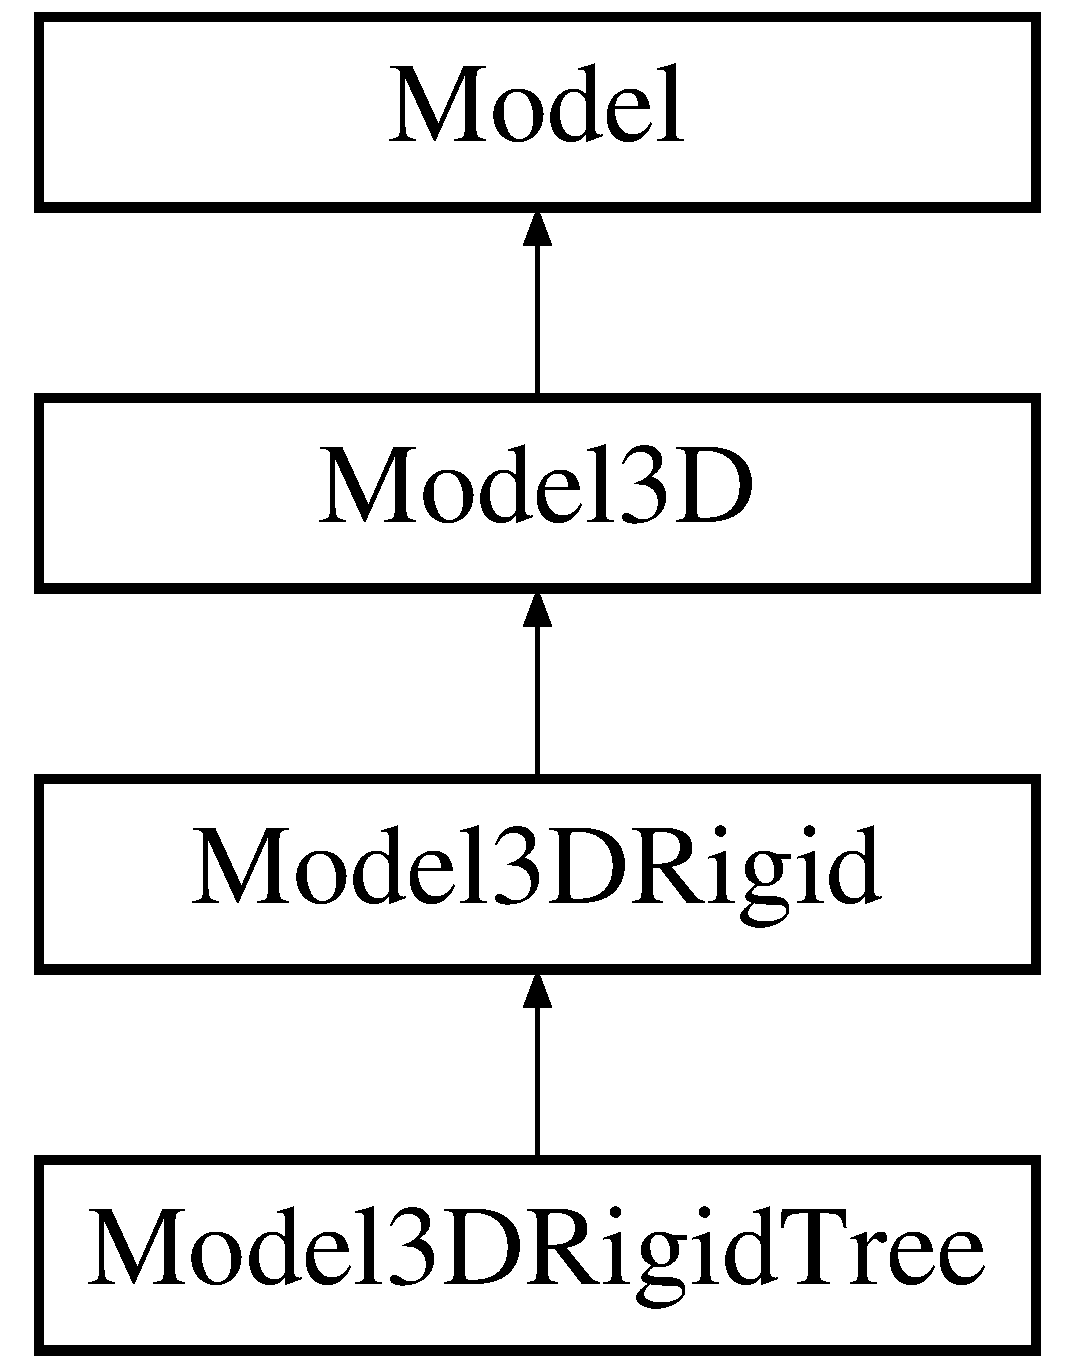
\includegraphics[height=4cm]{classModel3DRigidTree}
\end{center}
\end{figure}
\subsection*{Public Methods}
\begin{CompactItemize}
\item 
{\bf Model3DRigid\-Tree} (string path)
\item 
virtual {\bf $\sim$Model3DRigid\-Tree} ()
\item 
virtual {\bf MSLVector} {\bf State\-Transition\-Equation} (const {\bf MSLVector} \&x, const {\bf MSLVector} \&u)
\begin{CompactList}\small\item\em The state transition equation, or equations of motion, xdot=f(x,u).\item\end{CompactList}\item 
virtual {\bf MSLVector} {\bf State\-To\-Configuration} (const {\bf MSLVector} \&x)
\begin{CompactList}\small\item\em A method that converts a {\bf Model} {\rm (p.\,\pageref{classModel})} state in to a {\bf Geom} {\rm (p.\,\pageref{classGeom})} configuration.\item\end{CompactList}\item 
virtual {\bf MSLVector} {\bf Linear\-Interpolate} (const {\bf MSLVector} \&x1, const {\bf MSLVector} \&x2, const double \&a)
\begin{CompactList}\small\item\em Linearly interpolate two state while respecting topology.\item\end{CompactList}\item 
virtual double {\bf Metric} (const {\bf MSLVector} \&x1, const {\bf MSLVector} \&x2)
\begin{CompactList}\small\item\em A distance metric, which is Euclidean in the base class.\item\end{CompactList}\item 
virtual bool {\bf Satisfied} (const {\bf MSLVector} \&x)
\begin{CompactList}\small\item\em Test whether global state-space constraints are satisfied.\item\end{CompactList}\end{CompactItemize}
\subsection*{Public Attributes}
\begin{CompactItemize}
\item 
int {\bf Num\-Bodies}
\begin{CompactList}\small\item\em Number of bodies in the tree.\item\end{CompactList}\item 
{\bf MSLVector} {\bf DH}
\begin{CompactList}\small\item\em The distances between joints (\char`\"{}a\char`\"{} parameters in kinematics).\item\end{CompactList}\item 
vector$<$int$>$ {\bf State\-Indices}
\item 
vector$<$int$>$ {\bf Parents}
\end{CompactItemize}


\subsection{Detailed Description}
A 3D kinematic tree of bodies that uses DH parameters.

A 3D kinematic tree of bodies that uses DH parameters which should be given in a DH file in the following order: Alpha(1,2...), Theta(1,2...), A(1,2...), D(1,2...). Some of these parameters change during the movement, and each of these parameters becomes a state variable. The indices of these parameters should be given in the file State\-Indices (i.e., each entry corresponds to a state, and indicates which DH parameter is variable). For each body in the tree, the parent body in the tree should be indicated. This is specified in the file Parents. Each entry in Parents corresponds to a body (the i$^\wedge$th element is Robot i). The first entry is the root (this index is ignored because the root has no parent). The bodies in the tree must be arranged so that the indices in Parents are in nondecrreasing order (corresponding, for example to a depth-first search of the tree). 



\subsection{Constructor \& Destructor Documentation}
\index{Model3DRigidTree@{Model3DRigid\-Tree}!Model3DRigidTree@{Model3DRigidTree}}
\index{Model3DRigidTree@{Model3DRigidTree}!Model3DRigidTree@{Model3DRigid\-Tree}}
\subsubsection{\setlength{\rightskip}{0pt plus 5cm}Model3DRigid\-Tree::Model3DRigid\-Tree (string {\em path} = \char`\"{}\char`\"{})}\label{classModel3DRigidTree_a0}


\index{Model3DRigidTree@{Model3DRigid\-Tree}!~Model3DRigidTree@{$\sim$Model3DRigidTree}}
\index{~Model3DRigidTree@{$\sim$Model3DRigidTree}!Model3DRigidTree@{Model3DRigid\-Tree}}
\subsubsection{\setlength{\rightskip}{0pt plus 5cm}Model3DRigid\-Tree::$\sim$Model3DRigid\-Tree ()\hspace{0.3cm}{\tt  [inline, virtual]}}\label{classModel3DRigidTree_a1}




\subsection{Member Function Documentation}
\index{Model3DRigidTree@{Model3DRigid\-Tree}!LinearInterpolate@{LinearInterpolate}}
\index{LinearInterpolate@{LinearInterpolate}!Model3DRigidTree@{Model3DRigid\-Tree}}
\subsubsection{\setlength{\rightskip}{0pt plus 5cm}{\bf MSLVector} Model3DRigid\-Tree::Linear\-Interpolate (const {\bf MSLVector} \& {\em x1}, const {\bf MSLVector} \& {\em x2}, const double \& {\em a})\hspace{0.3cm}{\tt  [virtual]}}\label{classModel3DRigidTree_a4}


Linearly interpolate two state while respecting topology.

If a=0, then x1 is returned; if a=1, then x2 is returned. All intermediate values of \$a $\backslash$in [0,1]\$ yield intermediate states. This method is defined by {\bf Model} {\rm (p.\,\pageref{classModel})}. 

Reimplemented from {\bf Model3DRigid} {\rm (p.\,\pageref{classModel3DRigid_a5})}.\index{Model3DRigidTree@{Model3DRigid\-Tree}!Metric@{Metric}}
\index{Metric@{Metric}!Model3DRigidTree@{Model3DRigid\-Tree}}
\subsubsection{\setlength{\rightskip}{0pt plus 5cm}double Model3DRigid\-Tree::Metric (const {\bf MSLVector} \& {\em x1}, const {\bf MSLVector} \& {\em x2})\hspace{0.3cm}{\tt  [virtual]}}\label{classModel3DRigidTree_a5}


A distance metric, which is Euclidean in the base class.



Reimplemented from {\bf Model3DRigid} {\rm (p.\,\pageref{classModel3DRigid_a4})}.\index{Model3DRigidTree@{Model3DRigid\-Tree}!Satisfied@{Satisfied}}
\index{Satisfied@{Satisfied}!Model3DRigidTree@{Model3DRigid\-Tree}}
\subsubsection{\setlength{\rightskip}{0pt plus 5cm}bool Model3DRigid\-Tree::Satisfied (const {\bf MSLVector} \& {\em x})\hspace{0.3cm}{\tt  [virtual]}}\label{classModel3DRigidTree_a6}


Test whether global state-space constraints are satisfied.



Reimplemented from {\bf Model} {\rm (p.\,\pageref{classModel_a4})}.\index{Model3DRigidTree@{Model3DRigid\-Tree}!StateToConfiguration@{StateToConfiguration}}
\index{StateToConfiguration@{StateToConfiguration}!Model3DRigidTree@{Model3DRigid\-Tree}}
\subsubsection{\setlength{\rightskip}{0pt plus 5cm}{\bf MSLVector} Model3DRigid\-Tree::State\-To\-Configuration (const {\bf MSLVector} \& {\em x})\hspace{0.3cm}{\tt  [virtual]}}\label{classModel3DRigidTree_a3}


A method that converts a {\bf Model} {\rm (p.\,\pageref{classModel})} state in to a {\bf Geom} {\rm (p.\,\pageref{classGeom})} configuration.



Reimplemented from {\bf Model} {\rm (p.\,\pageref{classModel_a8})}.\index{Model3DRigidTree@{Model3DRigid\-Tree}!StateTransitionEquation@{StateTransitionEquation}}
\index{StateTransitionEquation@{StateTransitionEquation}!Model3DRigidTree@{Model3DRigid\-Tree}}
\subsubsection{\setlength{\rightskip}{0pt plus 5cm}{\bf MSLVector} Model3DRigid\-Tree::State\-Transition\-Equation (const {\bf MSLVector} \& {\em x}, const {\bf MSLVector} \& {\em u})\hspace{0.3cm}{\tt  [virtual]}}\label{classModel3DRigidTree_a2}


The state transition equation, or equations of motion, xdot=f(x,u).



Reimplemented from {\bf Model3DRigid} {\rm (p.\,\pageref{classModel3DRigid_a3})}.

\subsection{Member Data Documentation}
\index{Model3DRigidTree@{Model3DRigid\-Tree}!DH@{DH}}
\index{DH@{DH}!Model3DRigidTree@{Model3DRigid\-Tree}}
\subsubsection{\setlength{\rightskip}{0pt plus 5cm}{\bf MSLVector} Model3DRigid\-Tree::DH}\label{classModel3DRigidTree_m1}


The distances between joints (\char`\"{}a\char`\"{} parameters in kinematics).

\index{Model3DRigidTree@{Model3DRigid\-Tree}!NumBodies@{NumBodies}}
\index{NumBodies@{NumBodies}!Model3DRigidTree@{Model3DRigid\-Tree}}
\subsubsection{\setlength{\rightskip}{0pt plus 5cm}int Model3DRigid\-Tree::Num\-Bodies}\label{classModel3DRigidTree_m0}


Number of bodies in the tree.

\index{Model3DRigidTree@{Model3DRigid\-Tree}!Parents@{Parents}}
\index{Parents@{Parents}!Model3DRigidTree@{Model3DRigid\-Tree}}
\subsubsection{\setlength{\rightskip}{0pt plus 5cm}vector$<$ int $>$ Model3DRigid\-Tree::Parents$<$int$>$}\label{classModel3DRigidTree_m3}


\index{Model3DRigidTree@{Model3DRigid\-Tree}!StateIndices@{StateIndices}}
\index{StateIndices@{StateIndices}!Model3DRigidTree@{Model3DRigid\-Tree}}
\subsubsection{\setlength{\rightskip}{0pt plus 5cm}vector$<$ int $>$ Model3DRigid\-Tree::State\-Indices$<$int$>$}\label{classModel3DRigidTree_m2}




The documentation for this class was generated from the following files:\begin{CompactItemize}
\item 
{\bf model3d.h}\item 
{\bf model3d.C}\end{CompactItemize}

\section{Model\-Car  Class Reference}
\label{classModelCar}\index{ModelCar@{Model\-Car}}
The same model as {\bf Model2DRigid\-Car} {\rm (p.\,\pageref{classModel2DRigidCar})}. 


{\tt \#include $<$modelcar.h$>$}

Inheritance diagram for Model\-Car::\begin{figure}[H]
\begin{center}
\leavevmode
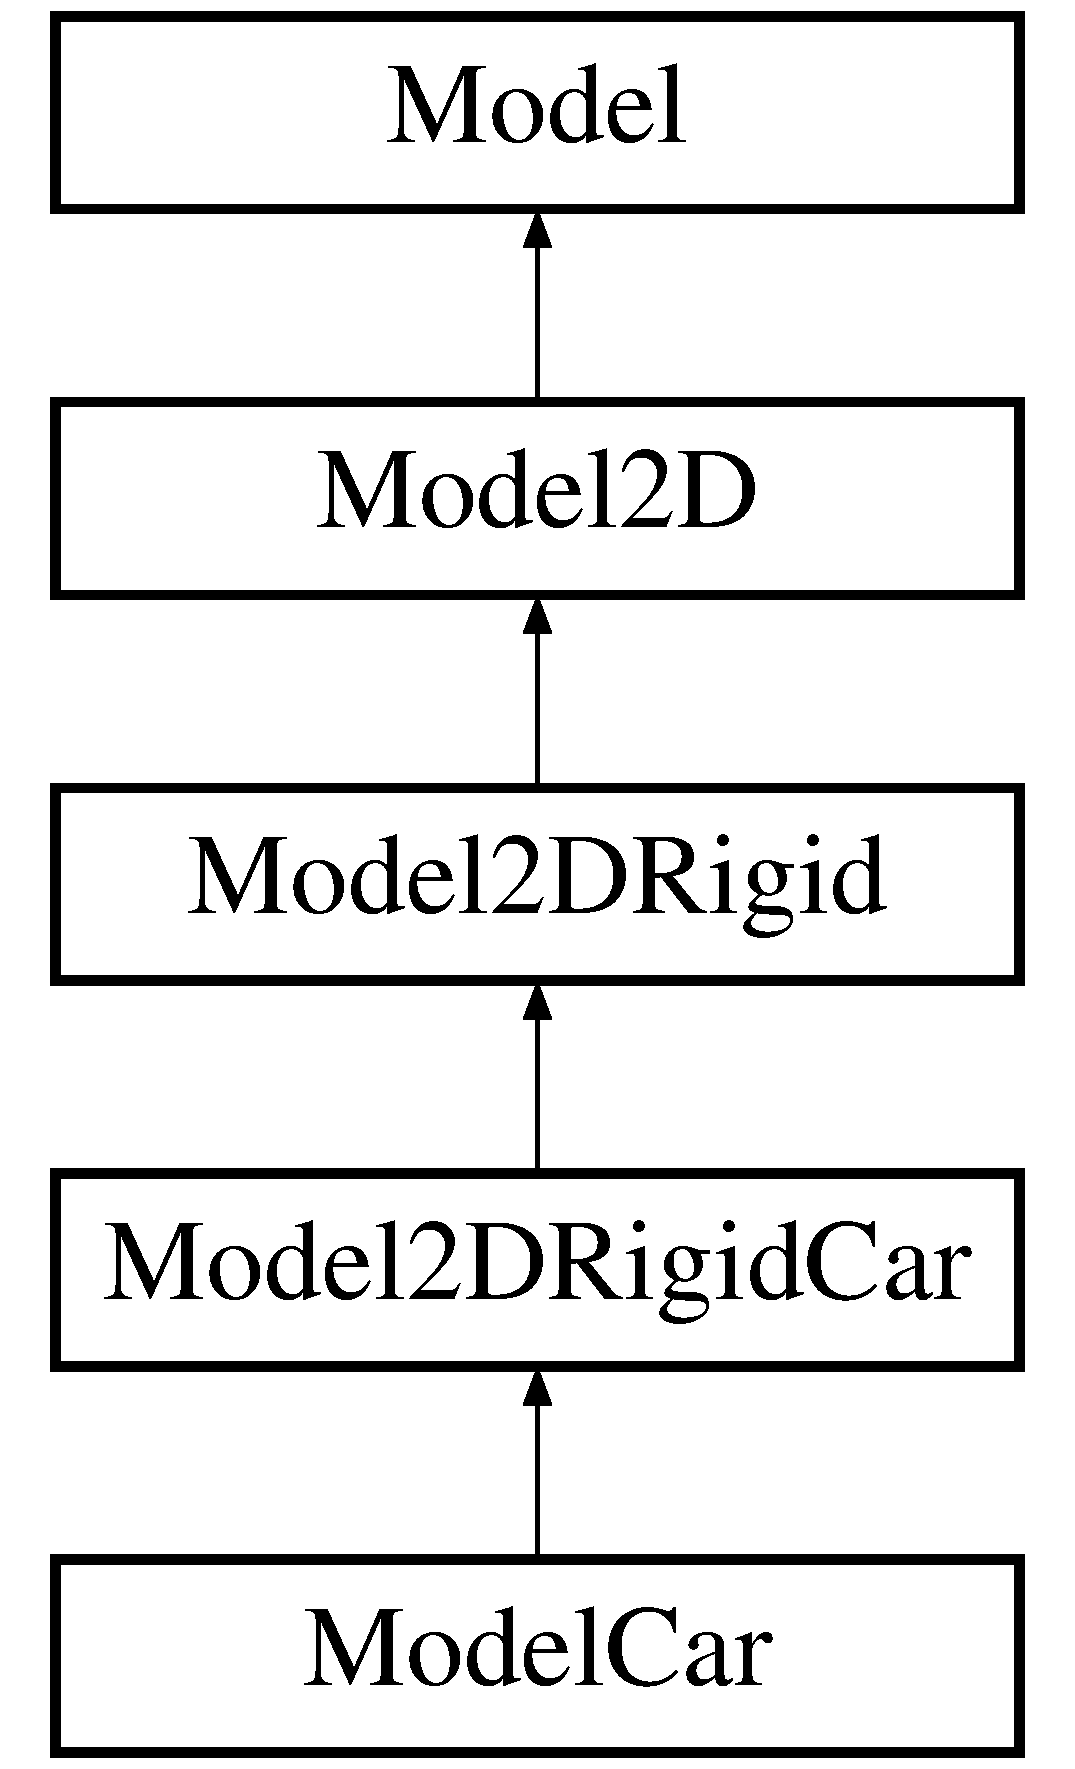
\includegraphics[height=5cm]{classModelCar}
\end{center}
\end{figure}
\subsection*{Public Methods}
\begin{CompactItemize}
\item 
{\bf Model\-Car} (string path)
\item 
virtual {\bf $\sim$Model\-Car} ()
\item 
virtual {\bf MSLVector} {\bf State\-To\-Configuration} (const {\bf MSLVector} \&x)
\begin{CompactList}\small\item\em A method that converts a {\bf Model} {\rm (p.\,\pageref{classModel})} state in to a {\bf Geom} {\rm (p.\,\pageref{classGeom})} configuration.\item\end{CompactList}\item 
virtual bool {\bf Satisfied} (const {\bf MSLVector} \&state)
\begin{CompactList}\small\item\em Test whether global state-space constraints are satisfied.\item\end{CompactList}\end{CompactItemize}
\subsection*{Public Attributes}
\begin{CompactItemize}
\item 
double {\bf Speed}
\end{CompactItemize}


\subsection{Detailed Description}
The same model as {\bf Model2DRigid\-Car} {\rm (p.\,\pageref{classModel2DRigidCar})}.



\subsection{Constructor \& Destructor Documentation}
\index{ModelCar@{Model\-Car}!ModelCar@{ModelCar}}
\index{ModelCar@{ModelCar}!ModelCar@{Model\-Car}}
\subsubsection{\setlength{\rightskip}{0pt plus 5cm}Model\-Car::Model\-Car (string {\em path} = \char`\"{}\char`\"{})}\label{classModelCar_a0}


\index{ModelCar@{Model\-Car}!~ModelCar@{$\sim$ModelCar}}
\index{~ModelCar@{$\sim$ModelCar}!ModelCar@{Model\-Car}}
\subsubsection{\setlength{\rightskip}{0pt plus 5cm}Model\-Car::$\sim$Model\-Car ()\hspace{0.3cm}{\tt  [inline, virtual]}}\label{classModelCar_a1}




\subsection{Member Function Documentation}
\index{ModelCar@{Model\-Car}!Satisfied@{Satisfied}}
\index{Satisfied@{Satisfied}!ModelCar@{Model\-Car}}
\subsubsection{\setlength{\rightskip}{0pt plus 5cm}bool Model\-Car::Satisfied (const {\bf MSLVector} \& {\em state})\hspace{0.3cm}{\tt  [virtual]}}\label{classModelCar_a3}


Test whether global state-space constraints are satisfied.



Reimplemented from {\bf Model} {\rm (p.\,\pageref{classModel_a4})}.\index{ModelCar@{Model\-Car}!StateToConfiguration@{StateToConfiguration}}
\index{StateToConfiguration@{StateToConfiguration}!ModelCar@{Model\-Car}}
\subsubsection{\setlength{\rightskip}{0pt plus 5cm}{\bf MSLVector} Model\-Car::State\-To\-Configuration (const {\bf MSLVector} \& {\em x})\hspace{0.3cm}{\tt  [virtual]}}\label{classModelCar_a2}


A method that converts a {\bf Model} {\rm (p.\,\pageref{classModel})} state in to a {\bf Geom} {\rm (p.\,\pageref{classGeom})} configuration.



Reimplemented from {\bf Model2DRigid} {\rm (p.\,\pageref{classModel2DRigid_a6})}.

\subsection{Member Data Documentation}
\index{ModelCar@{Model\-Car}!Speed@{Speed}}
\index{Speed@{Speed}!ModelCar@{Model\-Car}}
\subsubsection{\setlength{\rightskip}{0pt plus 5cm}double Model\-Car::Speed}\label{classModelCar_m0}




The documentation for this class was generated from the following files:\begin{CompactItemize}
\item 
{\bf modelcar.h}\item 
{\bf modelcar.C}\end{CompactItemize}

\section{Model\-Car\-Dyn  Class Reference}
\label{classModelCarDyn}\index{ModelCarDyn@{Model\-Car\-Dyn}}
The same model as {\bf Model2DRigid\-Dyncar} {\rm (p.\,\pageref{classModel2DRigidDyncar})}. 


{\tt \#include $<$modelcar.h$>$}

Inheritance diagram for Model\-Car\-Dyn::\begin{figure}[H]
\begin{center}
\leavevmode
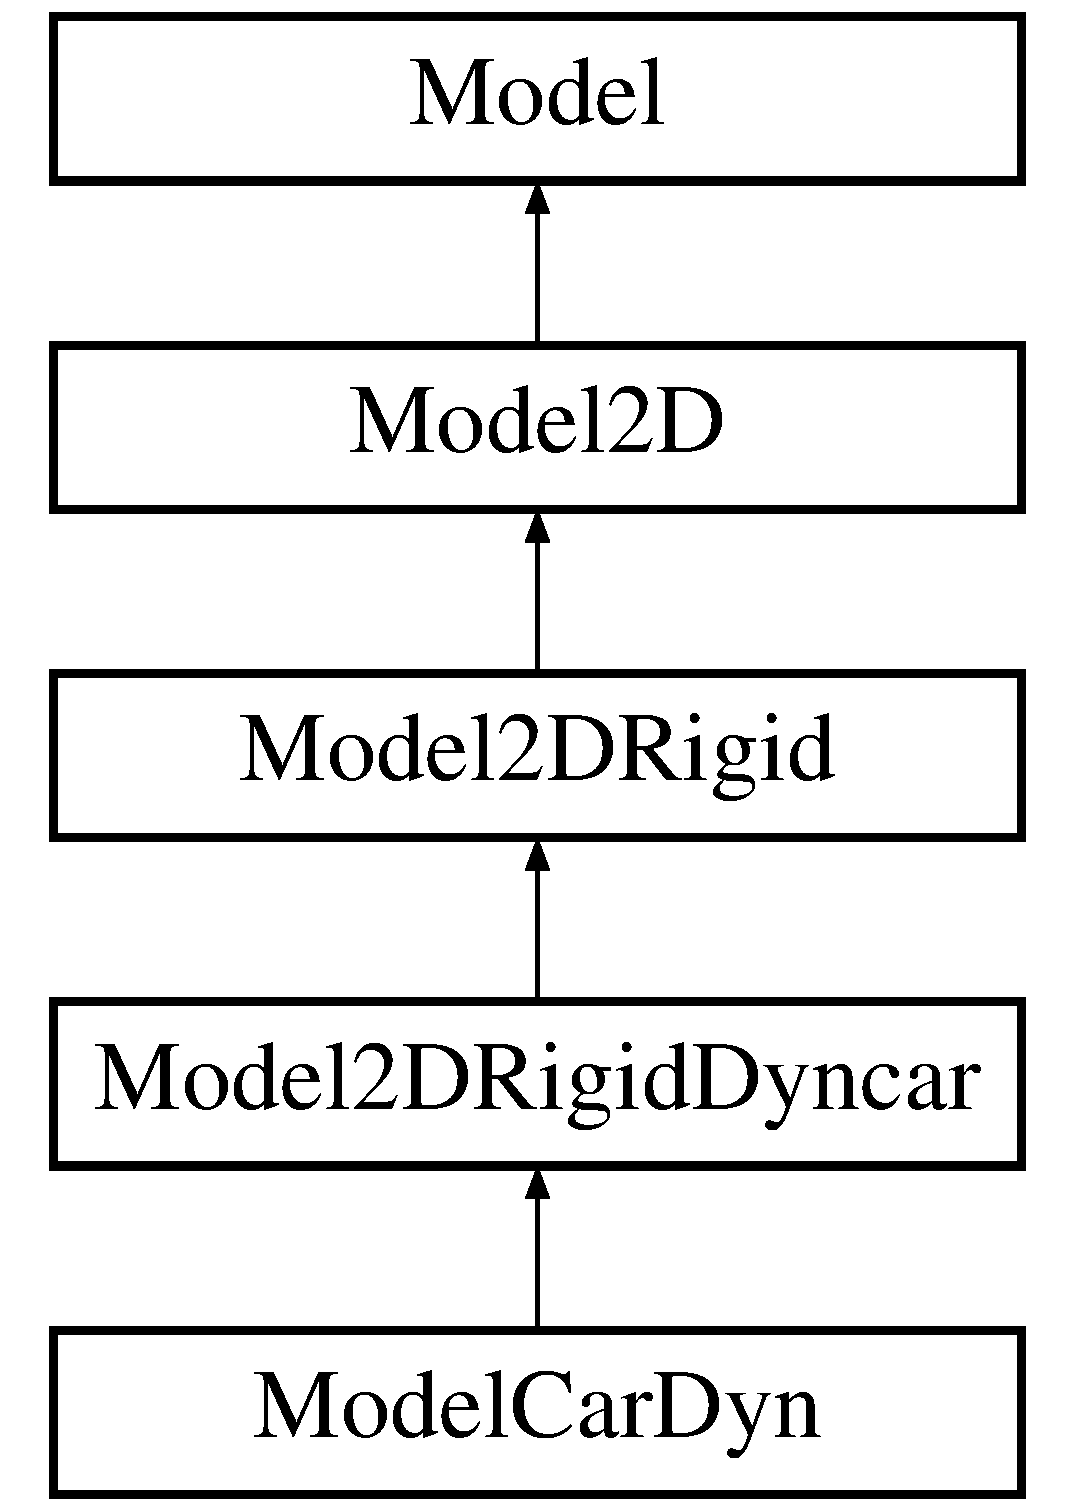
\includegraphics[height=5cm]{classModelCarDyn}
\end{center}
\end{figure}
\subsection*{Public Methods}
\begin{CompactItemize}
\item 
{\bf Model\-Car\-Dyn} (string path)
\item 
virtual {\bf $\sim$Model\-Car\-Dyn} ()
\item 
virtual {\bf MSLVector} {\bf State\-To\-Configuration} (const {\bf MSLVector} \&x)
\begin{CompactList}\small\item\em A method that converts a {\bf Model} {\rm (p.\,\pageref{classModel})} state in to a {\bf Geom} {\rm (p.\,\pageref{classGeom})} configuration.\item\end{CompactList}\item 
virtual double {\bf Metric} (const {\bf MSLVector} \&x1, const {\bf MSLVector} \&x2)
\begin{CompactList}\small\item\em A distance metric, which is Euclidean in the base class.\item\end{CompactList}\end{CompactItemize}


\subsection{Detailed Description}
The same model as {\bf Model2DRigid\-Dyncar} {\rm (p.\,\pageref{classModel2DRigidDyncar})}.



\subsection{Constructor \& Destructor Documentation}
\index{ModelCarDyn@{Model\-Car\-Dyn}!ModelCarDyn@{ModelCarDyn}}
\index{ModelCarDyn@{ModelCarDyn}!ModelCarDyn@{Model\-Car\-Dyn}}
\subsubsection{\setlength{\rightskip}{0pt plus 5cm}Model\-Car\-Dyn::Model\-Car\-Dyn (string {\em path} = \char`\"{}\char`\"{})}\label{classModelCarDyn_a0}


\index{ModelCarDyn@{Model\-Car\-Dyn}!~ModelCarDyn@{$\sim$ModelCarDyn}}
\index{~ModelCarDyn@{$\sim$ModelCarDyn}!ModelCarDyn@{Model\-Car\-Dyn}}
\subsubsection{\setlength{\rightskip}{0pt plus 5cm}Model\-Car\-Dyn::$\sim$Model\-Car\-Dyn ()\hspace{0.3cm}{\tt  [inline, virtual]}}\label{classModelCarDyn_a1}




\subsection{Member Function Documentation}
\index{ModelCarDyn@{Model\-Car\-Dyn}!Metric@{Metric}}
\index{Metric@{Metric}!ModelCarDyn@{Model\-Car\-Dyn}}
\subsubsection{\setlength{\rightskip}{0pt plus 5cm}double Model\-Car\-Dyn::Metric (const {\bf MSLVector} \& {\em x1}, const {\bf MSLVector} \& {\em x2})\hspace{0.3cm}{\tt  [virtual]}}\label{classModelCarDyn_a3}


A distance metric, which is Euclidean in the base class.



Reimplemented from {\bf Model2DRigid\-Dyncar} {\rm (p.\,\pageref{classModel2DRigidDyncar_a5})}.\index{ModelCarDyn@{Model\-Car\-Dyn}!StateToConfiguration@{StateToConfiguration}}
\index{StateToConfiguration@{StateToConfiguration}!ModelCarDyn@{Model\-Car\-Dyn}}
\subsubsection{\setlength{\rightskip}{0pt plus 5cm}{\bf MSLVector} Model\-Car\-Dyn::State\-To\-Configuration (const {\bf MSLVector} \& {\em x})\hspace{0.3cm}{\tt  [virtual]}}\label{classModelCarDyn_a2}


A method that converts a {\bf Model} {\rm (p.\,\pageref{classModel})} state in to a {\bf Geom} {\rm (p.\,\pageref{classGeom})} configuration.



Reimplemented from {\bf Model2DRigid\-Dyncar} {\rm (p.\,\pageref{classModel2DRigidDyncar_a3})}.

The documentation for this class was generated from the following files:\begin{CompactItemize}
\item 
{\bf modelcar.h}\item 
{\bf modelcar.C}\end{CompactItemize}

\section{Model\-Car\-Dyn\-Ntire  Class Reference}
\label{classModelCarDynNtire}\index{ModelCarDynNtire@{Model\-Car\-Dyn\-Ntire}}
The same model as {\bf Model2DRigid\-Dyncar\-Ntire} {\rm (p.\,\pageref{classModel2DRigidDyncarNtire})}. 


{\tt \#include $<$modelcar.h$>$}

Inheritance diagram for Model\-Car\-Dyn\-Ntire::\begin{figure}[H]
\begin{center}
\leavevmode
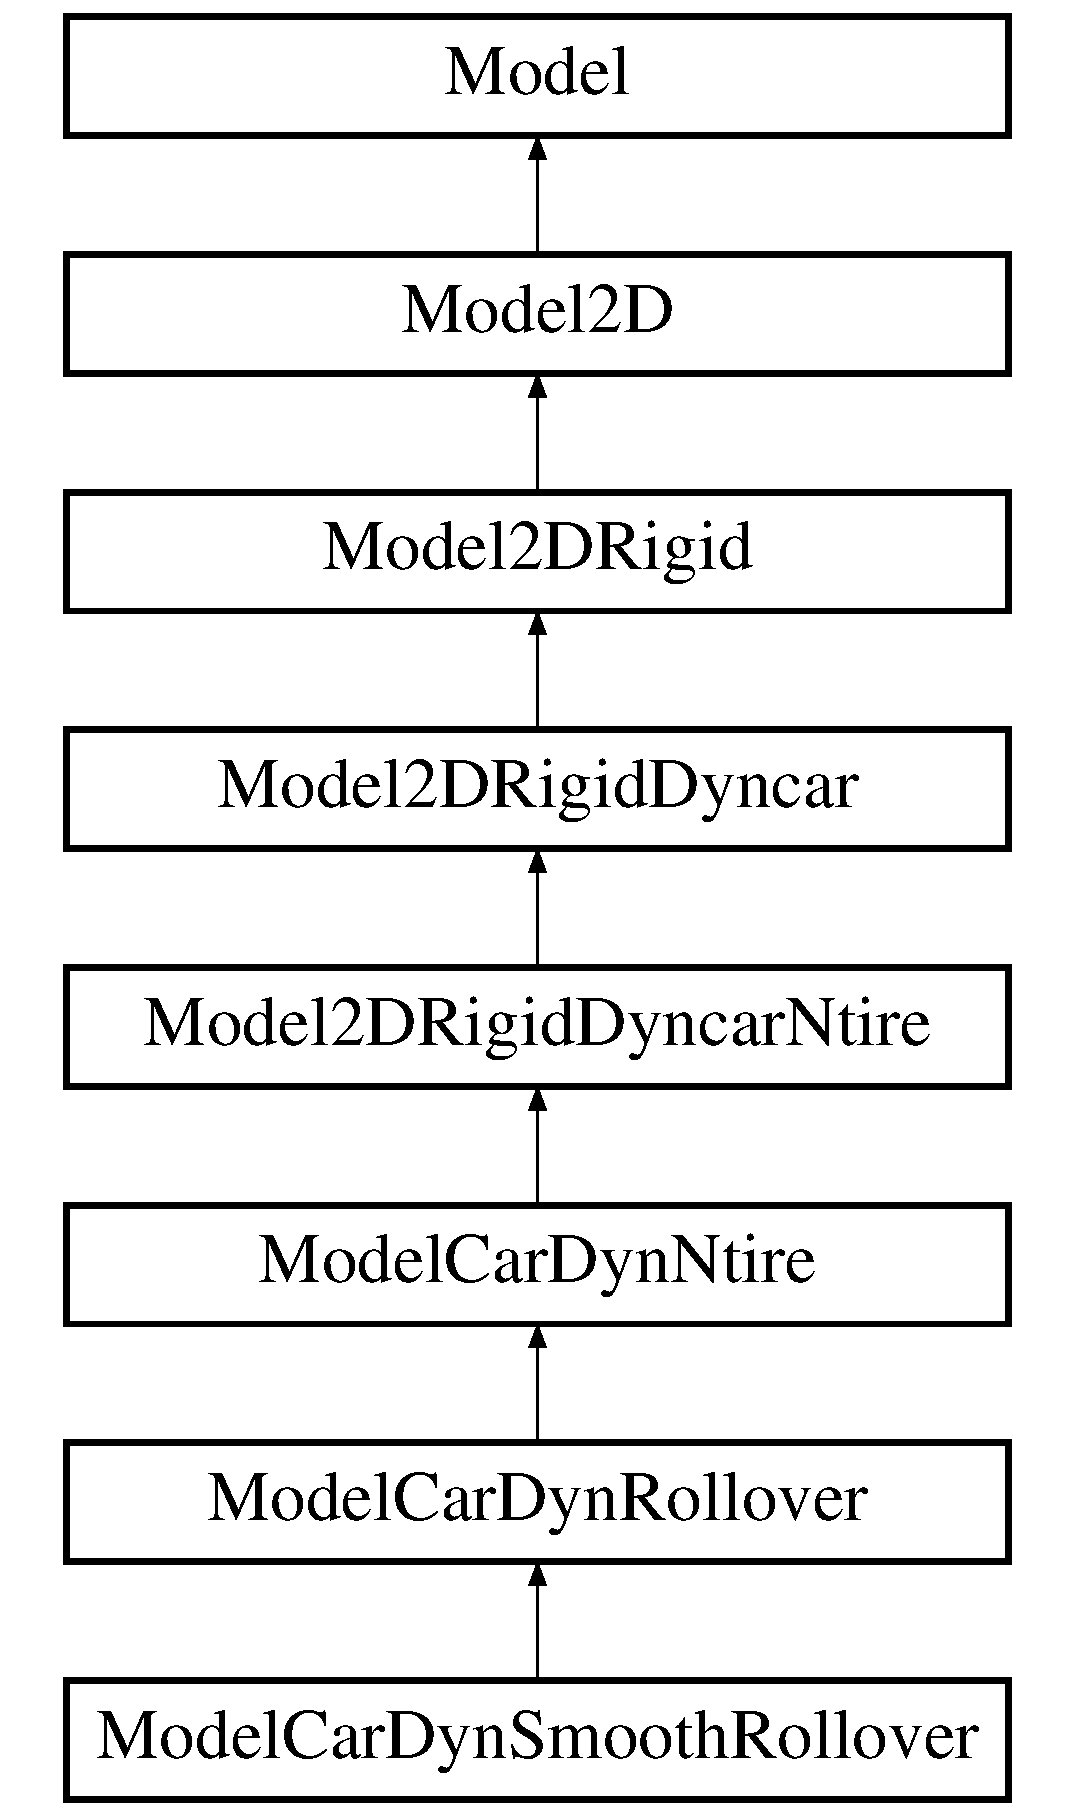
\includegraphics[height=8cm]{classModelCarDynNtire}
\end{center}
\end{figure}
\subsection*{Public Methods}
\begin{CompactItemize}
\item 
{\bf Model\-Car\-Dyn\-Ntire} (string path)
\item 
virtual {\bf $\sim$Model\-Car\-Dyn\-Ntire} ()
\item 
virtual {\bf MSLVector} {\bf State\-To\-Configuration} (const {\bf MSLVector} \&x)
\begin{CompactList}\small\item\em A method that converts a {\bf Model} {\rm (p.\,\pageref{classModel})} state in to a {\bf Geom} {\rm (p.\,\pageref{classGeom})} configuration.\item\end{CompactList}\item 
virtual double {\bf Metric} (const {\bf MSLVector} \&x1, const {\bf MSLVector} \&x2)
\begin{CompactList}\small\item\em A distance metric, which is Euclidean in the base class.\item\end{CompactList}\end{CompactItemize}


\subsection{Detailed Description}
The same model as {\bf Model2DRigid\-Dyncar\-Ntire} {\rm (p.\,\pageref{classModel2DRigidDyncarNtire})}.



\subsection{Constructor \& Destructor Documentation}
\index{ModelCarDynNtire@{Model\-Car\-Dyn\-Ntire}!ModelCarDynNtire@{ModelCarDynNtire}}
\index{ModelCarDynNtire@{ModelCarDynNtire}!ModelCarDynNtire@{Model\-Car\-Dyn\-Ntire}}
\subsubsection{\setlength{\rightskip}{0pt plus 5cm}Model\-Car\-Dyn\-Ntire::Model\-Car\-Dyn\-Ntire (string {\em path} = \char`\"{}\char`\"{})}\label{classModelCarDynNtire_a0}


\index{ModelCarDynNtire@{Model\-Car\-Dyn\-Ntire}!~ModelCarDynNtire@{$\sim$ModelCarDynNtire}}
\index{~ModelCarDynNtire@{$\sim$ModelCarDynNtire}!ModelCarDynNtire@{Model\-Car\-Dyn\-Ntire}}
\subsubsection{\setlength{\rightskip}{0pt plus 5cm}Model\-Car\-Dyn\-Ntire::$\sim$Model\-Car\-Dyn\-Ntire ()\hspace{0.3cm}{\tt  [inline, virtual]}}\label{classModelCarDynNtire_a1}




\subsection{Member Function Documentation}
\index{ModelCarDynNtire@{Model\-Car\-Dyn\-Ntire}!Metric@{Metric}}
\index{Metric@{Metric}!ModelCarDynNtire@{Model\-Car\-Dyn\-Ntire}}
\subsubsection{\setlength{\rightskip}{0pt plus 5cm}double Model\-Car\-Dyn\-Ntire::Metric (const {\bf MSLVector} \& {\em x1}, const {\bf MSLVector} \& {\em x2})\hspace{0.3cm}{\tt  [virtual]}}\label{classModelCarDynNtire_a3}


A distance metric, which is Euclidean in the base class.



Reimplemented from {\bf Model2DRigid\-Dyncar} {\rm (p.\,\pageref{classModel2DRigidDyncar_a5})}.

Reimplemented in {\bf Model\-Car\-Dyn\-Rollover} {\rm (p.\,\pageref{classModelCarDynRollover_a6})}, and {\bf Model\-Car\-Dyn\-Smooth\-Rollover} {\rm (p.\,\pageref{classModelCarDynSmoothRollover_a4})}.\index{ModelCarDynNtire@{Model\-Car\-Dyn\-Ntire}!StateToConfiguration@{StateToConfiguration}}
\index{StateToConfiguration@{StateToConfiguration}!ModelCarDynNtire@{Model\-Car\-Dyn\-Ntire}}
\subsubsection{\setlength{\rightskip}{0pt plus 5cm}{\bf MSLVector} Model\-Car\-Dyn\-Ntire::State\-To\-Configuration (const {\bf MSLVector} \& {\em x})\hspace{0.3cm}{\tt  [virtual]}}\label{classModelCarDynNtire_a2}


A method that converts a {\bf Model} {\rm (p.\,\pageref{classModel})} state in to a {\bf Geom} {\rm (p.\,\pageref{classGeom})} configuration.



Reimplemented from {\bf Model2DRigid\-Dyncar} {\rm (p.\,\pageref{classModel2DRigidDyncar_a3})}.

Reimplemented in {\bf Model\-Car\-Dyn\-Rollover} {\rm (p.\,\pageref{classModelCarDynRollover_a4})}, and {\bf Model\-Car\-Dyn\-Smooth\-Rollover} {\rm (p.\,\pageref{classModelCarDynSmoothRollover_a3})}.

The documentation for this class was generated from the following files:\begin{CompactItemize}
\item 
{\bf modelcar.h}\item 
{\bf modelcar.C}\end{CompactItemize}

\section{Model\-Car\-Dyn\-Rollover  Class Reference}
\label{classModelCarDynRollover}\index{ModelCarDynRollover@{Model\-Car\-Dyn\-Rollover}}
A car model considering the rolling effect and the pressure on different tires of the car is different. If the pressure on one tire is 0, the car is considered rolling over. The pressure model of the tire is rigid such that pressure can change at instant time, which means: (1) It might be the reason that only forward {\bf RRT} {\rm (p.\,\pageref{classRRT})} tree works. (2) In the Select\-Input function, pressure has to be restored when to test new inputs. 


{\tt \#include $<$modelcar.h$>$}

Inheritance diagram for Model\-Car\-Dyn\-Rollover::\begin{figure}[H]
\begin{center}
\leavevmode
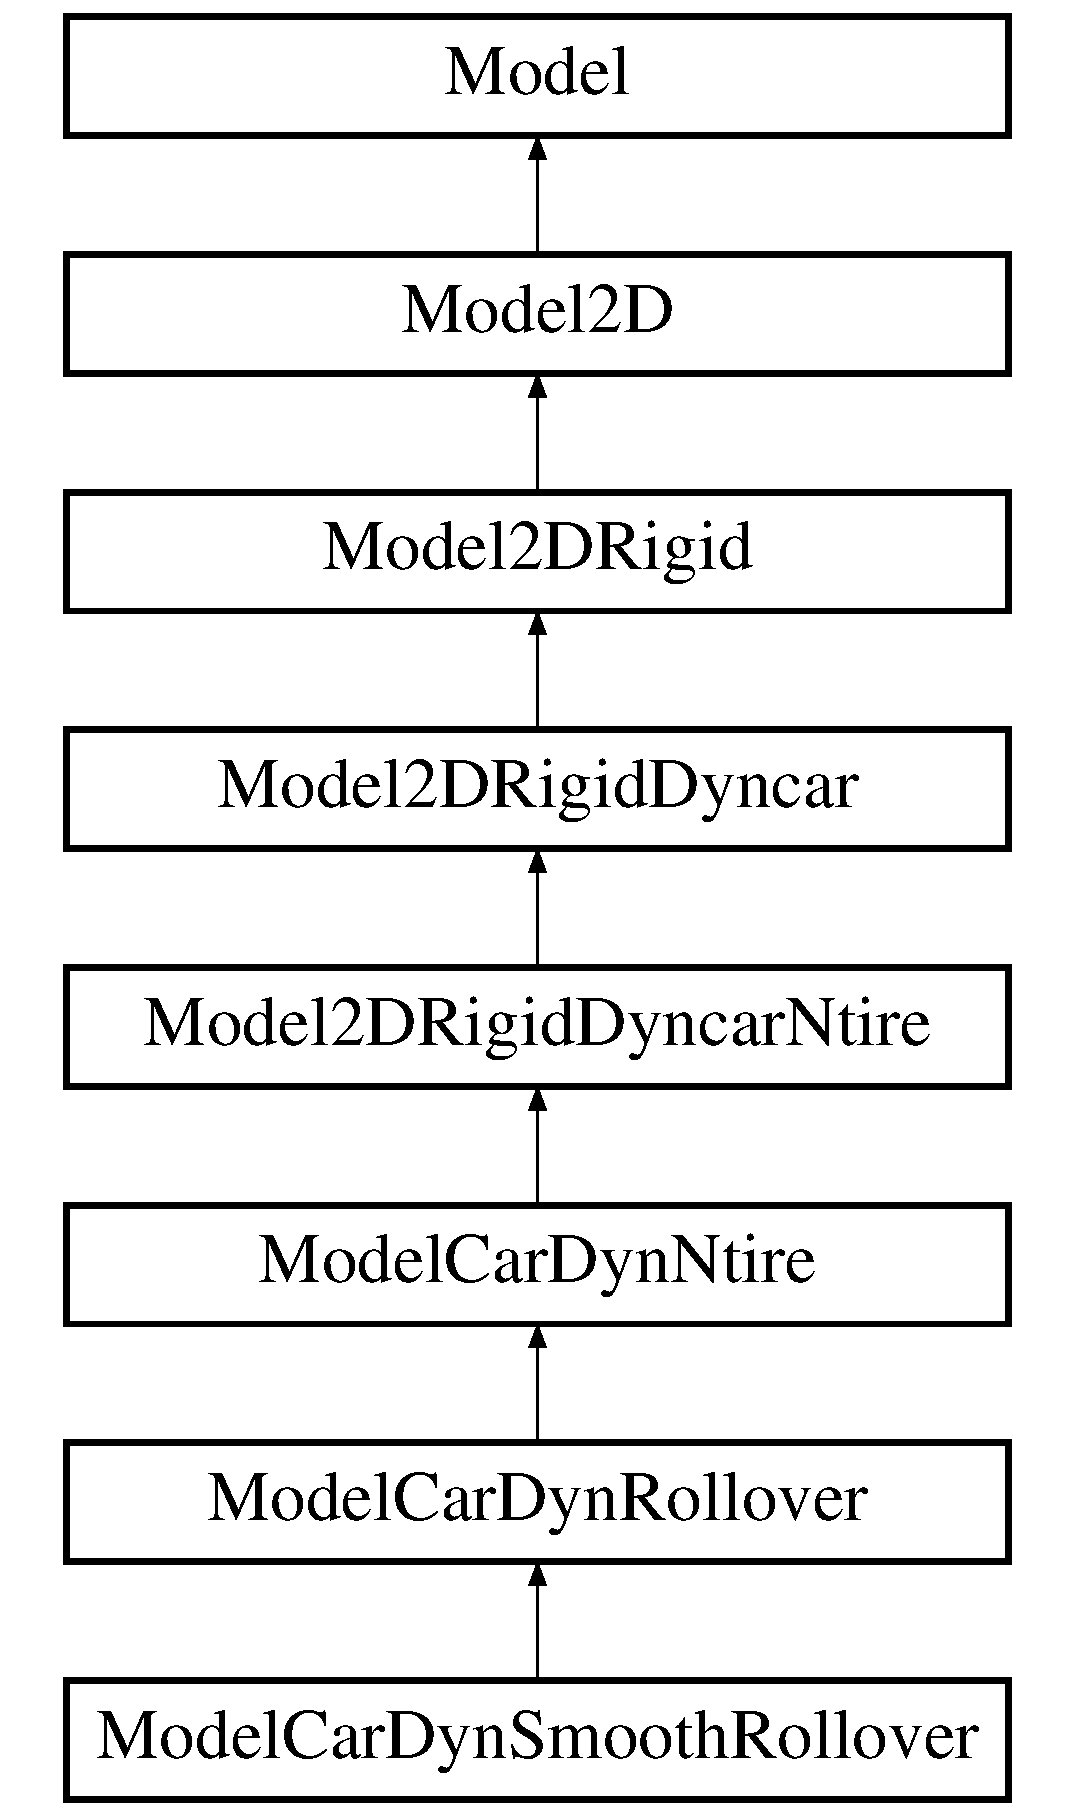
\includegraphics[height=8cm]{classModelCarDynRollover}
\end{center}
\end{figure}
\subsection*{Public Methods}
\begin{CompactItemize}
\item 
{\bf Model\-Car\-Dyn\-Rollover} (string path)
\item 
virtual {\bf $\sim$Model\-Car\-Dyn\-Rollover} ()
\item 
int {\bf sgn} (double {\bf x})
\item 
virtual {\bf MSLVector} {\bf State\-Transition\-Equation} (const {\bf MSLVector} \&x1, const {\bf MSLVector} \&u)
\begin{CompactList}\small\item\em The state transition equation, or equations of motion, xdot=f(x,u).\item\end{CompactList}\item 
virtual {\bf MSLVector} {\bf State\-To\-Configuration} (const {\bf MSLVector} \&{\bf x})
\begin{CompactList}\small\item\em A method that converts a {\bf Model} {\rm (p.\,\pageref{classModel})} state in to a {\bf Geom} {\rm (p.\,\pageref{classGeom})} configuration.\item\end{CompactList}\item 
virtual {\bf MSLVector} {\bf Integrate} (const {\bf MSLVector} \&{\bf x}, const {\bf MSLVector} \&u, const double \&h)
\begin{CompactList}\small\item\em !!!!!!!! It has both the state and the uncontrolled state.\item\end{CompactList}\item 
virtual double {\bf Metric} (const {\bf MSLVector} \&x1, const {\bf MSLVector} \&x2)
\begin{CompactList}\small\item\em A distance metric, which is Euclidean in the base class.\item\end{CompactList}\item 
bool {\bf Roll\-Over\-Free} (const {\bf MSLVector} \&{\bf x})
\item 
bool {\bf Satisfied} (const {\bf MSLVector} \&{\bf x})
\begin{CompactList}\small\item\em Test whether global state-space constraints are satisfied.\item\end{CompactList}\end{CompactItemize}
\subsection*{Public Attributes}
\begin{CompactItemize}
\item 
double {\bf K}
\item 
double {\bf c}
\item 
double {\bf Ixx}
\item 
double {\bf T}
\item 
double {\bf H}
\item 
double {\bf H2}
\item 
double {\bf Ms}
\item 
double {\bf Wn}
\item 
double {\bf Fai}
\item 
double {\bf x}
\item 
bool {\bf Is\-Roll\-Over}
\end{CompactItemize}


\subsection{Detailed Description}
A car model considering the rolling effect and the pressure on different tires of the car is different. If the pressure on one tire is 0, the car is considered rolling over. The pressure model of the tire is rigid such that pressure can change at instant time, which means: (1) It might be the reason that only forward {\bf RRT} {\rm (p.\,\pageref{classRRT})} tree works. (2) In the Select\-Input function, pressure has to be restored when to test new inputs.



\subsection{Constructor \& Destructor Documentation}
\index{ModelCarDynRollover@{Model\-Car\-Dyn\-Rollover}!ModelCarDynRollover@{ModelCarDynRollover}}
\index{ModelCarDynRollover@{ModelCarDynRollover}!ModelCarDynRollover@{Model\-Car\-Dyn\-Rollover}}
\subsubsection{\setlength{\rightskip}{0pt plus 5cm}Model\-Car\-Dyn\-Rollover::Model\-Car\-Dyn\-Rollover (string {\em path} = \char`\"{}\char`\"{})}\label{classModelCarDynRollover_a0}


\index{ModelCarDynRollover@{Model\-Car\-Dyn\-Rollover}!~ModelCarDynRollover@{$\sim$ModelCarDynRollover}}
\index{~ModelCarDynRollover@{$\sim$ModelCarDynRollover}!ModelCarDynRollover@{Model\-Car\-Dyn\-Rollover}}
\subsubsection{\setlength{\rightskip}{0pt plus 5cm}Model\-Car\-Dyn\-Rollover::$\sim$Model\-Car\-Dyn\-Rollover ()\hspace{0.3cm}{\tt  [inline, virtual]}}\label{classModelCarDynRollover_a1}




\subsection{Member Function Documentation}
\index{ModelCarDynRollover@{Model\-Car\-Dyn\-Rollover}!Integrate@{Integrate}}
\index{Integrate@{Integrate}!ModelCarDynRollover@{Model\-Car\-Dyn\-Rollover}}
\subsubsection{\setlength{\rightskip}{0pt plus 5cm}{\bf MSLVector} Model\-Car\-Dyn\-Rollover::Integrate (const {\bf MSLVector} \& {\em x}, const {\bf MSLVector} \& {\em u}, const double \& {\em h})\hspace{0.3cm}{\tt  [virtual]}}\label{classModelCarDynRollover_a5}


!!!!!!!! It has both the state and the uncontrolled state.



Reimplemented from {\bf Model2DRigid\-Dyncar} {\rm (p.\,\pageref{classModel2DRigidDyncar_a2})}.\index{ModelCarDynRollover@{Model\-Car\-Dyn\-Rollover}!Metric@{Metric}}
\index{Metric@{Metric}!ModelCarDynRollover@{Model\-Car\-Dyn\-Rollover}}
\subsubsection{\setlength{\rightskip}{0pt plus 5cm}double Model\-Car\-Dyn\-Rollover::Metric (const {\bf MSLVector} \& {\em x1}, const {\bf MSLVector} \& {\em x2})\hspace{0.3cm}{\tt  [virtual]}}\label{classModelCarDynRollover_a6}


A distance metric, which is Euclidean in the base class.



Reimplemented from {\bf Model\-Car\-Dyn\-Ntire} {\rm (p.\,\pageref{classModelCarDynNtire_a3})}.

Reimplemented in {\bf Model\-Car\-Dyn\-Smooth\-Rollover} {\rm (p.\,\pageref{classModelCarDynSmoothRollover_a4})}.\index{ModelCarDynRollover@{Model\-Car\-Dyn\-Rollover}!RollOverFree@{RollOverFree}}
\index{RollOverFree@{RollOverFree}!ModelCarDynRollover@{Model\-Car\-Dyn\-Rollover}}
\subsubsection{\setlength{\rightskip}{0pt plus 5cm}bool Model\-Car\-Dyn\-Rollover::Roll\-Over\-Free (const {\bf MSLVector} \& {\em x})}\label{classModelCarDynRollover_a7}


\index{ModelCarDynRollover@{Model\-Car\-Dyn\-Rollover}!Satisfied@{Satisfied}}
\index{Satisfied@{Satisfied}!ModelCarDynRollover@{Model\-Car\-Dyn\-Rollover}}
\subsubsection{\setlength{\rightskip}{0pt plus 5cm}bool Model\-Car\-Dyn\-Rollover::Satisfied (const {\bf MSLVector} \& {\em x})\hspace{0.3cm}{\tt  [virtual]}}\label{classModelCarDynRollover_a8}


Test whether global state-space constraints are satisfied.



Reimplemented from {\bf Model} {\rm (p.\,\pageref{classModel_a4})}.\index{ModelCarDynRollover@{Model\-Car\-Dyn\-Rollover}!StateToConfiguration@{StateToConfiguration}}
\index{StateToConfiguration@{StateToConfiguration}!ModelCarDynRollover@{Model\-Car\-Dyn\-Rollover}}
\subsubsection{\setlength{\rightskip}{0pt plus 5cm}{\bf MSLVector} Model\-Car\-Dyn\-Rollover::State\-To\-Configuration (const {\bf MSLVector} \& {\em x})\hspace{0.3cm}{\tt  [virtual]}}\label{classModelCarDynRollover_a4}


A method that converts a {\bf Model} {\rm (p.\,\pageref{classModel})} state in to a {\bf Geom} {\rm (p.\,\pageref{classGeom})} configuration.



Reimplemented from {\bf Model\-Car\-Dyn\-Ntire} {\rm (p.\,\pageref{classModelCarDynNtire_a2})}.

Reimplemented in {\bf Model\-Car\-Dyn\-Smooth\-Rollover} {\rm (p.\,\pageref{classModelCarDynSmoothRollover_a3})}.\index{ModelCarDynRollover@{Model\-Car\-Dyn\-Rollover}!StateTransitionEquation@{StateTransitionEquation}}
\index{StateTransitionEquation@{StateTransitionEquation}!ModelCarDynRollover@{Model\-Car\-Dyn\-Rollover}}
\subsubsection{\setlength{\rightskip}{0pt plus 5cm}{\bf MSLVector} Model\-Car\-Dyn\-Rollover::State\-Transition\-Equation (const {\bf MSLVector} \& {\em x1}, const {\bf MSLVector} \& {\em u})\hspace{0.3cm}{\tt  [virtual]}}\label{classModelCarDynRollover_a3}


The state transition equation, or equations of motion, xdot=f(x,u).



Reimplemented from {\bf Model2DRigid\-Dyncar\-Ntire} {\rm (p.\,\pageref{classModel2DRigidDyncarNtire_a2})}.

Reimplemented in {\bf Model\-Car\-Dyn\-Smooth\-Rollover} {\rm (p.\,\pageref{classModelCarDynSmoothRollover_a2})}.\index{ModelCarDynRollover@{Model\-Car\-Dyn\-Rollover}!sgn@{sgn}}
\index{sgn@{sgn}!ModelCarDynRollover@{Model\-Car\-Dyn\-Rollover}}
\subsubsection{\setlength{\rightskip}{0pt plus 5cm}int Model\-Car\-Dyn\-Rollover::sgn (double {\em x})}\label{classModelCarDynRollover_a2}




\subsection{Member Data Documentation}
\index{ModelCarDynRollover@{Model\-Car\-Dyn\-Rollover}!Fai@{Fai}}
\index{Fai@{Fai}!ModelCarDynRollover@{Model\-Car\-Dyn\-Rollover}}
\subsubsection{\setlength{\rightskip}{0pt plus 5cm}double Model\-Car\-Dyn\-Rollover::Fai}\label{classModelCarDynRollover_m8}


\index{ModelCarDynRollover@{Model\-Car\-Dyn\-Rollover}!H@{H}}
\index{H@{H}!ModelCarDynRollover@{Model\-Car\-Dyn\-Rollover}}
\subsubsection{\setlength{\rightskip}{0pt plus 5cm}double Model\-Car\-Dyn\-Rollover::H}\label{classModelCarDynRollover_m4}


\index{ModelCarDynRollover@{Model\-Car\-Dyn\-Rollover}!H2@{H2}}
\index{H2@{H2}!ModelCarDynRollover@{Model\-Car\-Dyn\-Rollover}}
\subsubsection{\setlength{\rightskip}{0pt plus 5cm}double Model\-Car\-Dyn\-Rollover::H2}\label{classModelCarDynRollover_m5}


\index{ModelCarDynRollover@{Model\-Car\-Dyn\-Rollover}!IsRollOver@{IsRollOver}}
\index{IsRollOver@{IsRollOver}!ModelCarDynRollover@{Model\-Car\-Dyn\-Rollover}}
\subsubsection{\setlength{\rightskip}{0pt plus 5cm}bool Model\-Car\-Dyn\-Rollover::Is\-Roll\-Over}\label{classModelCarDynRollover_m10}


\index{ModelCarDynRollover@{Model\-Car\-Dyn\-Rollover}!Ixx@{Ixx}}
\index{Ixx@{Ixx}!ModelCarDynRollover@{Model\-Car\-Dyn\-Rollover}}
\subsubsection{\setlength{\rightskip}{0pt plus 5cm}double Model\-Car\-Dyn\-Rollover::Ixx}\label{classModelCarDynRollover_m2}


\index{ModelCarDynRollover@{Model\-Car\-Dyn\-Rollover}!K@{K}}
\index{K@{K}!ModelCarDynRollover@{Model\-Car\-Dyn\-Rollover}}
\subsubsection{\setlength{\rightskip}{0pt plus 5cm}double Model\-Car\-Dyn\-Rollover::K}\label{classModelCarDynRollover_m0}


\index{ModelCarDynRollover@{Model\-Car\-Dyn\-Rollover}!Ms@{Ms}}
\index{Ms@{Ms}!ModelCarDynRollover@{Model\-Car\-Dyn\-Rollover}}
\subsubsection{\setlength{\rightskip}{0pt plus 5cm}double Model\-Car\-Dyn\-Rollover::Ms}\label{classModelCarDynRollover_m6}


\index{ModelCarDynRollover@{Model\-Car\-Dyn\-Rollover}!T@{T}}
\index{T@{T}!ModelCarDynRollover@{Model\-Car\-Dyn\-Rollover}}
\subsubsection{\setlength{\rightskip}{0pt plus 5cm}double Model\-Car\-Dyn\-Rollover::T}\label{classModelCarDynRollover_m3}


\index{ModelCarDynRollover@{Model\-Car\-Dyn\-Rollover}!Wn@{Wn}}
\index{Wn@{Wn}!ModelCarDynRollover@{Model\-Car\-Dyn\-Rollover}}
\subsubsection{\setlength{\rightskip}{0pt plus 5cm}double Model\-Car\-Dyn\-Rollover::Wn}\label{classModelCarDynRollover_m7}


\index{ModelCarDynRollover@{Model\-Car\-Dyn\-Rollover}!c@{c}}
\index{c@{c}!ModelCarDynRollover@{Model\-Car\-Dyn\-Rollover}}
\subsubsection{\setlength{\rightskip}{0pt plus 5cm}double Model\-Car\-Dyn\-Rollover::c}\label{classModelCarDynRollover_m1}


\index{ModelCarDynRollover@{Model\-Car\-Dyn\-Rollover}!x@{x}}
\index{x@{x}!ModelCarDynRollover@{Model\-Car\-Dyn\-Rollover}}
\subsubsection{\setlength{\rightskip}{0pt plus 5cm}double Model\-Car\-Dyn\-Rollover::x}\label{classModelCarDynRollover_m9}




The documentation for this class was generated from the following files:\begin{CompactItemize}
\item 
{\bf modelcar.h}\item 
{\bf modelcar.C}\end{CompactItemize}

\section{Model\-Car\-Dyn\-Smooth\-Rollover  Class Reference}
\label{classModelCarDynSmoothRollover}\index{ModelCarDynSmoothRollover@{Model\-Car\-Dyn\-Smooth\-Rollover}}
One more dimension than {\bf Model\-Car\-Dyn\-Rollover} {\rm (p.\,\pageref{classModelCarDynRollover})} considering the steering angle can only change continuously. 


{\tt \#include $<$modelcar.h$>$}

Inheritance diagram for Model\-Car\-Dyn\-Smooth\-Rollover::\begin{figure}[H]
\begin{center}
\leavevmode
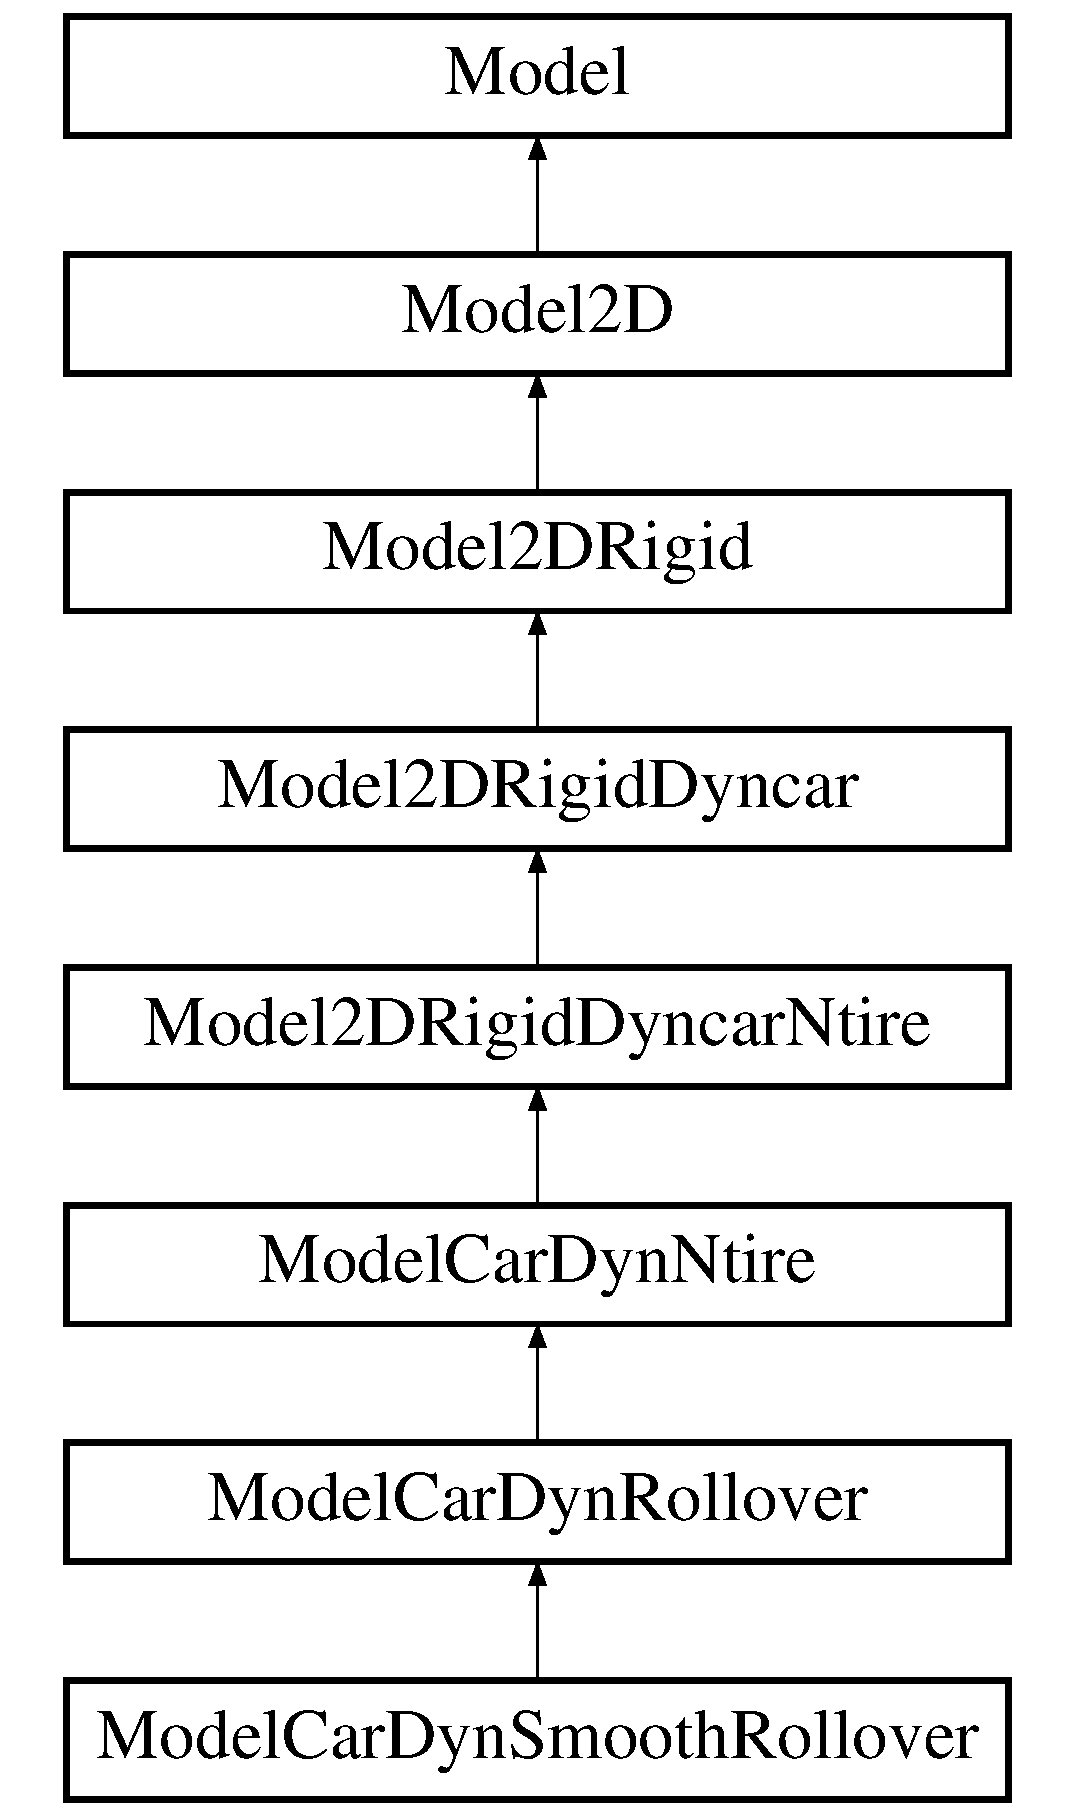
\includegraphics[height=8cm]{classModelCarDynSmoothRollover}
\end{center}
\end{figure}
\subsection*{Public Methods}
\begin{CompactItemize}
\item 
{\bf Model\-Car\-Dyn\-Smooth\-Rollover} (string path)
\item 
virtual {\bf $\sim$Model\-Car\-Dyn\-Smooth\-Rollover} ()
\item 
virtual {\bf MSLVector} {\bf State\-Transition\-Equation} (const {\bf MSLVector} \&x1, const {\bf MSLVector} \&u)
\begin{CompactList}\small\item\em The state transition equation, or equations of motion, xdot=f(x,u).\item\end{CompactList}\item 
virtual {\bf MSLVector} {\bf State\-To\-Configuration} (const {\bf MSLVector} \&{\bf x})
\begin{CompactList}\small\item\em A method that converts a {\bf Model} {\rm (p.\,\pageref{classModel})} state in to a {\bf Geom} {\rm (p.\,\pageref{classGeom})} configuration.\item\end{CompactList}\item 
virtual double {\bf Metric} (const {\bf MSLVector} \&x1, const {\bf MSLVector} \&x2)
\begin{CompactList}\small\item\em A distance metric, which is Euclidean in the base class.\item\end{CompactList}\item 
virtual {\bf MSLVector} {\bf Linear\-Interpolate} (const {\bf MSLVector} \&x1, const {\bf MSLVector} \&x2, const double \&a)
\begin{CompactList}\small\item\em Linearly interpolate two state while respecting topology.\item\end{CompactList}\end{CompactItemize}


\subsection{Detailed Description}
One more dimension than {\bf Model\-Car\-Dyn\-Rollover} {\rm (p.\,\pageref{classModelCarDynRollover})} considering the steering angle can only change continuously.



\subsection{Constructor \& Destructor Documentation}
\index{ModelCarDynSmoothRollover@{Model\-Car\-Dyn\-Smooth\-Rollover}!ModelCarDynSmoothRollover@{ModelCarDynSmoothRollover}}
\index{ModelCarDynSmoothRollover@{ModelCarDynSmoothRollover}!ModelCarDynSmoothRollover@{Model\-Car\-Dyn\-Smooth\-Rollover}}
\subsubsection{\setlength{\rightskip}{0pt plus 5cm}Model\-Car\-Dyn\-Smooth\-Rollover::Model\-Car\-Dyn\-Smooth\-Rollover (string {\em path} = \char`\"{}\char`\"{})}\label{classModelCarDynSmoothRollover_a0}


\index{ModelCarDynSmoothRollover@{Model\-Car\-Dyn\-Smooth\-Rollover}!~ModelCarDynSmoothRollover@{$\sim$ModelCarDynSmoothRollover}}
\index{~ModelCarDynSmoothRollover@{$\sim$ModelCarDynSmoothRollover}!ModelCarDynSmoothRollover@{Model\-Car\-Dyn\-Smooth\-Rollover}}
\subsubsection{\setlength{\rightskip}{0pt plus 5cm}Model\-Car\-Dyn\-Smooth\-Rollover::$\sim$Model\-Car\-Dyn\-Smooth\-Rollover ()\hspace{0.3cm}{\tt  [inline, virtual]}}\label{classModelCarDynSmoothRollover_a1}




\subsection{Member Function Documentation}
\index{ModelCarDynSmoothRollover@{Model\-Car\-Dyn\-Smooth\-Rollover}!LinearInterpolate@{LinearInterpolate}}
\index{LinearInterpolate@{LinearInterpolate}!ModelCarDynSmoothRollover@{Model\-Car\-Dyn\-Smooth\-Rollover}}
\subsubsection{\setlength{\rightskip}{0pt plus 5cm}{\bf MSLVector} Model\-Car\-Dyn\-Smooth\-Rollover::Linear\-Interpolate (const {\bf MSLVector} \& {\em x1}, const {\bf MSLVector} \& {\em x2}, const double \& {\em a})\hspace{0.3cm}{\tt  [virtual]}}\label{classModelCarDynSmoothRollover_a5}


Linearly interpolate two state while respecting topology.

If a=0, then x1 is returned; if a=1, then x2 is returned. All intermediate values of \$a $\backslash$in [0,1]\$ yield intermediate states. This method is defined by {\bf Model} {\rm (p.\,\pageref{classModel})}. 

Reimplemented from {\bf Model2DRigid\-Dyncar} {\rm (p.\,\pageref{classModel2DRigidDyncar_a6})}.\index{ModelCarDynSmoothRollover@{Model\-Car\-Dyn\-Smooth\-Rollover}!Metric@{Metric}}
\index{Metric@{Metric}!ModelCarDynSmoothRollover@{Model\-Car\-Dyn\-Smooth\-Rollover}}
\subsubsection{\setlength{\rightskip}{0pt plus 5cm}double Model\-Car\-Dyn\-Smooth\-Rollover::Metric (const {\bf MSLVector} \& {\em x1}, const {\bf MSLVector} \& {\em x2})\hspace{0.3cm}{\tt  [virtual]}}\label{classModelCarDynSmoothRollover_a4}


A distance metric, which is Euclidean in the base class.



Reimplemented from {\bf Model\-Car\-Dyn\-Rollover} {\rm (p.\,\pageref{classModelCarDynRollover_a6})}.\index{ModelCarDynSmoothRollover@{Model\-Car\-Dyn\-Smooth\-Rollover}!StateToConfiguration@{StateToConfiguration}}
\index{StateToConfiguration@{StateToConfiguration}!ModelCarDynSmoothRollover@{Model\-Car\-Dyn\-Smooth\-Rollover}}
\subsubsection{\setlength{\rightskip}{0pt plus 5cm}{\bf MSLVector} Model\-Car\-Dyn\-Smooth\-Rollover::State\-To\-Configuration (const {\bf MSLVector} \& {\em x})\hspace{0.3cm}{\tt  [virtual]}}\label{classModelCarDynSmoothRollover_a3}


A method that converts a {\bf Model} {\rm (p.\,\pageref{classModel})} state in to a {\bf Geom} {\rm (p.\,\pageref{classGeom})} configuration.



Reimplemented from {\bf Model\-Car\-Dyn\-Rollover} {\rm (p.\,\pageref{classModelCarDynRollover_a4})}.\index{ModelCarDynSmoothRollover@{Model\-Car\-Dyn\-Smooth\-Rollover}!StateTransitionEquation@{StateTransitionEquation}}
\index{StateTransitionEquation@{StateTransitionEquation}!ModelCarDynSmoothRollover@{Model\-Car\-Dyn\-Smooth\-Rollover}}
\subsubsection{\setlength{\rightskip}{0pt plus 5cm}{\bf MSLVector} Model\-Car\-Dyn\-Smooth\-Rollover::State\-Transition\-Equation (const {\bf MSLVector} \& {\em x1}, const {\bf MSLVector} \& {\em u})\hspace{0.3cm}{\tt  [virtual]}}\label{classModelCarDynSmoothRollover_a2}


The state transition equation, or equations of motion, xdot=f(x,u).



Reimplemented from {\bf Model\-Car\-Dyn\-Rollover} {\rm (p.\,\pageref{classModelCarDynRollover_a3})}.

The documentation for this class was generated from the following files:\begin{CompactItemize}
\item 
{\bf modelcar.h}\item 
{\bf modelcar.C}\end{CompactItemize}

\section{Model\-Car\-Smooth  Class Reference}
\label{classModelCarSmooth}\index{ModelCarSmooth@{Model\-Car\-Smooth}}
The same model as {\bf Model2DRigid\-Car\-Smooth} {\rm (p.\,\pageref{classModel2DRigidCarSmooth})}. 


{\tt \#include $<$modelcar.h$>$}

Inheritance diagram for Model\-Car\-Smooth::\begin{figure}[H]
\begin{center}
\leavevmode
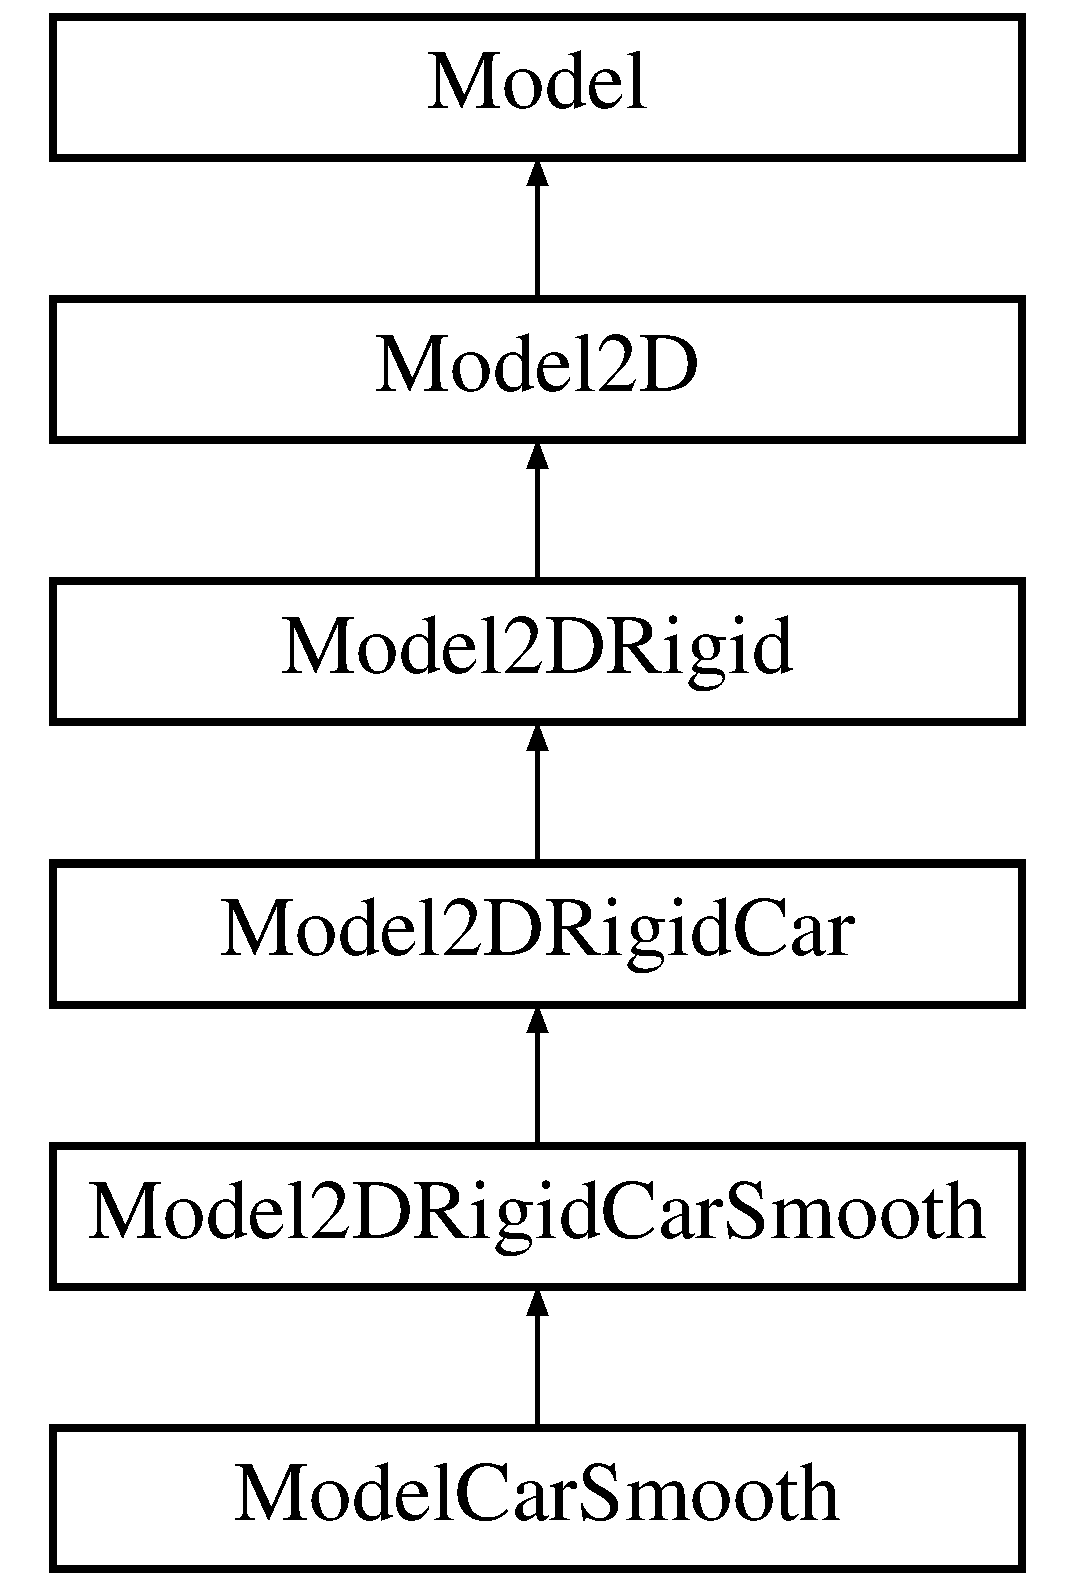
\includegraphics[height=6cm]{classModelCarSmooth}
\end{center}
\end{figure}
\subsection*{Public Methods}
\begin{CompactItemize}
\item 
{\bf Model\-Car\-Smooth} (string path)
\item 
virtual {\bf $\sim$Model\-Car\-Smooth} ()
\item 
virtual {\bf MSLVector} {\bf State\-To\-Configuration} (const {\bf MSLVector} \&x)
\begin{CompactList}\small\item\em A method that converts a {\bf Model} {\rm (p.\,\pageref{classModel})} state in to a {\bf Geom} {\rm (p.\,\pageref{classGeom})} configuration.\item\end{CompactList}\end{CompactItemize}


\subsection{Detailed Description}
The same model as {\bf Model2DRigid\-Car\-Smooth} {\rm (p.\,\pageref{classModel2DRigidCarSmooth})}.



\subsection{Constructor \& Destructor Documentation}
\index{ModelCarSmooth@{Model\-Car\-Smooth}!ModelCarSmooth@{ModelCarSmooth}}
\index{ModelCarSmooth@{ModelCarSmooth}!ModelCarSmooth@{Model\-Car\-Smooth}}
\subsubsection{\setlength{\rightskip}{0pt plus 5cm}Model\-Car\-Smooth::Model\-Car\-Smooth (string {\em path} = \char`\"{}\char`\"{})}\label{classModelCarSmooth_a0}


\index{ModelCarSmooth@{Model\-Car\-Smooth}!~ModelCarSmooth@{$\sim$ModelCarSmooth}}
\index{~ModelCarSmooth@{$\sim$ModelCarSmooth}!ModelCarSmooth@{Model\-Car\-Smooth}}
\subsubsection{\setlength{\rightskip}{0pt plus 5cm}Model\-Car\-Smooth::$\sim$Model\-Car\-Smooth ()\hspace{0.3cm}{\tt  [inline, virtual]}}\label{classModelCarSmooth_a1}




\subsection{Member Function Documentation}
\index{ModelCarSmooth@{Model\-Car\-Smooth}!StateToConfiguration@{StateToConfiguration}}
\index{StateToConfiguration@{StateToConfiguration}!ModelCarSmooth@{Model\-Car\-Smooth}}
\subsubsection{\setlength{\rightskip}{0pt plus 5cm}{\bf MSLVector} Model\-Car\-Smooth::State\-To\-Configuration (const {\bf MSLVector} \& {\em x})\hspace{0.3cm}{\tt  [virtual]}}\label{classModelCarSmooth_a2}


A method that converts a {\bf Model} {\rm (p.\,\pageref{classModel})} state in to a {\bf Geom} {\rm (p.\,\pageref{classGeom})} configuration.



Reimplemented from {\bf Model2DRigid\-Car\-Smooth} {\rm (p.\,\pageref{classModel2DRigidCarSmooth_a5})}.

The documentation for this class was generated from the following files:\begin{CompactItemize}
\item 
{\bf modelcar.h}\item 
{\bf modelcar.C}\end{CompactItemize}

\section{Model\-Linear  Class Reference}
\label{classModelLinear}\index{ModelLinear@{Model\-Linear}}
A linear systems model: xdot = Ax + Bu. 


{\tt \#include $<$modelmisc.h$>$}

Inheritance diagram for Model\-Linear::\begin{figure}[H]
\begin{center}
\leavevmode
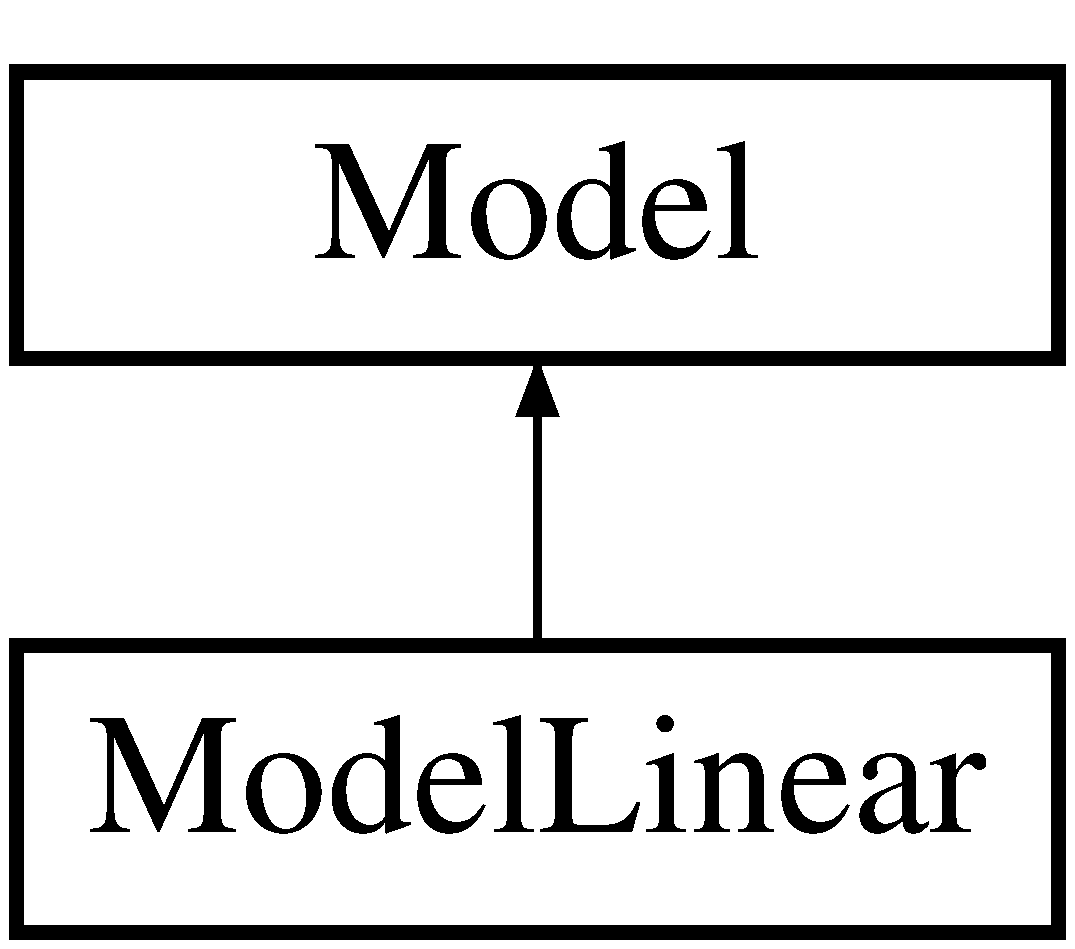
\includegraphics[height=2cm]{classModelLinear}
\end{center}
\end{figure}
\subsection*{Public Methods}
\begin{CompactItemize}
\item 
{\bf Model\-Linear} (string path)
\item 
virtual {\bf $\sim$Model\-Linear} ()
\item 
virtual {\bf MSLVector} {\bf State\-To\-Configuration} (const {\bf MSLVector} \&x)
\begin{CompactList}\small\item\em A method that converts a {\bf Model} {\rm (p.\,\pageref{classModel})} state in to a {\bf Geom} {\rm (p.\,\pageref{classGeom})} configuration.\item\end{CompactList}\item 
virtual {\bf MSLVector} {\bf Integrate} (const {\bf MSLVector} \&x, const {\bf MSLVector} \&u, const double \&h)
\begin{CompactList}\small\item\em Perform integration from state x, using input u, over time step h.\item\end{CompactList}\item 
virtual {\bf MSLVector} {\bf State\-Transition\-Equation} (const {\bf MSLVector} \&x, const {\bf MSLVector} \&u)
\begin{CompactList}\small\item\em The state transition equation, or equations of motion, xdot=f(x,u).\item\end{CompactList}\end{CompactItemize}
\subsection*{Public Attributes}
\begin{CompactItemize}
\item 
{\bf MSLMatrix} {\bf A}
\item 
{\bf MSLMatrix} {\bf B}
\end{CompactItemize}


\subsection{Detailed Description}
A linear systems model: xdot = Ax + Bu.



\subsection{Constructor \& Destructor Documentation}
\index{ModelLinear@{Model\-Linear}!ModelLinear@{ModelLinear}}
\index{ModelLinear@{ModelLinear}!ModelLinear@{Model\-Linear}}
\subsubsection{\setlength{\rightskip}{0pt plus 5cm}Model\-Linear::Model\-Linear (string {\em path} = \char`\"{}\char`\"{})}\label{classModelLinear_a0}


\index{ModelLinear@{Model\-Linear}!~ModelLinear@{$\sim$ModelLinear}}
\index{~ModelLinear@{$\sim$ModelLinear}!ModelLinear@{Model\-Linear}}
\subsubsection{\setlength{\rightskip}{0pt plus 5cm}Model\-Linear::$\sim$Model\-Linear ()\hspace{0.3cm}{\tt  [inline, virtual]}}\label{classModelLinear_a1}




\subsection{Member Function Documentation}
\index{ModelLinear@{Model\-Linear}!Integrate@{Integrate}}
\index{Integrate@{Integrate}!ModelLinear@{Model\-Linear}}
\subsubsection{\setlength{\rightskip}{0pt plus 5cm}{\bf MSLVector} Model\-Linear::Integrate (const {\bf MSLVector} \& {\em x}, const {\bf MSLVector} \& {\em u}, const double \& {\em h})\hspace{0.3cm}{\tt  [virtual]}}\label{classModelLinear_a3}


Perform integration from state x, using input u, over time step h.



Reimplemented from {\bf Model} {\rm (p.\,\pageref{classModel_a5})}.\index{ModelLinear@{Model\-Linear}!StateToConfiguration@{StateToConfiguration}}
\index{StateToConfiguration@{StateToConfiguration}!ModelLinear@{Model\-Linear}}
\subsubsection{\setlength{\rightskip}{0pt plus 5cm}{\bf MSLVector} Model\-Linear::State\-To\-Configuration (const {\bf MSLVector} \& {\em x})\hspace{0.3cm}{\tt  [virtual]}}\label{classModelLinear_a2}


A method that converts a {\bf Model} {\rm (p.\,\pageref{classModel})} state in to a {\bf Geom} {\rm (p.\,\pageref{classGeom})} configuration.



Reimplemented from {\bf Model} {\rm (p.\,\pageref{classModel_a8})}.\index{ModelLinear@{Model\-Linear}!StateTransitionEquation@{StateTransitionEquation}}
\index{StateTransitionEquation@{StateTransitionEquation}!ModelLinear@{Model\-Linear}}
\subsubsection{\setlength{\rightskip}{0pt plus 5cm}{\bf MSLVector} Model\-Linear::State\-Transition\-Equation (const {\bf MSLVector} \& {\em x}, const {\bf MSLVector} \& {\em u})\hspace{0.3cm}{\tt  [virtual]}}\label{classModelLinear_a4}


The state transition equation, or equations of motion, xdot=f(x,u).



Reimplemented from {\bf Model} {\rm (p.\,\pageref{classModel_a3})}.

\subsection{Member Data Documentation}
\index{ModelLinear@{Model\-Linear}!A@{A}}
\index{A@{A}!ModelLinear@{Model\-Linear}}
\subsubsection{\setlength{\rightskip}{0pt plus 5cm}{\bf MSLMatrix} Model\-Linear::A}\label{classModelLinear_m0}


\index{ModelLinear@{Model\-Linear}!B@{B}}
\index{B@{B}!ModelLinear@{Model\-Linear}}
\subsubsection{\setlength{\rightskip}{0pt plus 5cm}{\bf MSLMatrix} Model\-Linear::B}\label{classModelLinear_m1}




The documentation for this class was generated from the following files:\begin{CompactItemize}
\item 
{\bf modelmisc.h}\item 
{\bf modelmisc.C}\end{CompactItemize}

\section{Model\-ND  Class Reference}
\label{classModelND}\index{ModelND@{Model\-ND}}
Simple axis-parallel motions in an N-dimensional space. 


{\tt \#include $<$modelmisc.h$>$}

Inheritance diagram for Model\-ND::\begin{figure}[H]
\begin{center}
\leavevmode
\includegraphics[height=2cm]{classModelND}
\end{center}
\end{figure}
\subsection*{Public Methods}
\begin{CompactItemize}
\item 
{\bf Model\-ND} (string path)
\item 
virtual {\bf $\sim$Model\-ND} ()
\item 
virtual {\bf MSLVector} {\bf State\-To\-Configuration} (const {\bf MSLVector} \&x)
\begin{CompactList}\small\item\em A method that converts a {\bf Model} {\rm (p.\,\pageref{classModel})} state in to a {\bf Geom} {\rm (p.\,\pageref{classGeom})} configuration.\item\end{CompactList}\item 
virtual {\bf MSLVector} {\bf Integrate} (const {\bf MSLVector} \&x, const {\bf MSLVector} \&u, const double \&h)
\begin{CompactList}\small\item\em Perform integration from state x, using input u, over time step h.\item\end{CompactList}\item 
virtual {\bf MSLVector} {\bf State\-Transition\-Equation} (const {\bf MSLVector} \&x, const {\bf MSLVector} \&u)
\begin{CompactList}\small\item\em The state transition equation, or equations of motion, xdot=f(x,u).\item\end{CompactList}\end{CompactItemize}
\subsection*{Public Attributes}
\begin{CompactItemize}
\item 
double {\bf Corridor\-Width}
\end{CompactItemize}


\subsection{Detailed Description}
Simple axis-parallel motions in an N-dimensional space.



\subsection{Constructor \& Destructor Documentation}
\index{ModelND@{Model\-ND}!ModelND@{ModelND}}
\index{ModelND@{ModelND}!ModelND@{Model\-ND}}
\subsubsection{\setlength{\rightskip}{0pt plus 5cm}Model\-ND::Model\-ND (string {\em path} = \char`\"{}\char`\"{})}\label{classModelND_a0}


\index{ModelND@{Model\-ND}!~ModelND@{$\sim$ModelND}}
\index{~ModelND@{$\sim$ModelND}!ModelND@{Model\-ND}}
\subsubsection{\setlength{\rightskip}{0pt plus 5cm}Model\-ND::$\sim$Model\-ND ()\hspace{0.3cm}{\tt  [inline, virtual]}}\label{classModelND_a1}




\subsection{Member Function Documentation}
\index{ModelND@{Model\-ND}!Integrate@{Integrate}}
\index{Integrate@{Integrate}!ModelND@{Model\-ND}}
\subsubsection{\setlength{\rightskip}{0pt plus 5cm}{\bf MSLVector} Model\-ND::Integrate (const {\bf MSLVector} \& {\em x}, const {\bf MSLVector} \& {\em u}, const double \& {\em h})\hspace{0.3cm}{\tt  [virtual]}}\label{classModelND_a3}


Perform integration from state x, using input u, over time step h.



Reimplemented from {\bf Model} {\rm (p.\,\pageref{classModel_a5})}.\index{ModelND@{Model\-ND}!StateToConfiguration@{StateToConfiguration}}
\index{StateToConfiguration@{StateToConfiguration}!ModelND@{Model\-ND}}
\subsubsection{\setlength{\rightskip}{0pt plus 5cm}{\bf MSLVector} Model\-ND::State\-To\-Configuration (const {\bf MSLVector} \& {\em x})\hspace{0.3cm}{\tt  [virtual]}}\label{classModelND_a2}


A method that converts a {\bf Model} {\rm (p.\,\pageref{classModel})} state in to a {\bf Geom} {\rm (p.\,\pageref{classGeom})} configuration.



Reimplemented from {\bf Model} {\rm (p.\,\pageref{classModel_a8})}.\index{ModelND@{Model\-ND}!StateTransitionEquation@{StateTransitionEquation}}
\index{StateTransitionEquation@{StateTransitionEquation}!ModelND@{Model\-ND}}
\subsubsection{\setlength{\rightskip}{0pt plus 5cm}{\bf MSLVector} Model\-ND::State\-Transition\-Equation (const {\bf MSLVector} \& {\em x}, const {\bf MSLVector} \& {\em u})\hspace{0.3cm}{\tt  [virtual]}}\label{classModelND_a4}


The state transition equation, or equations of motion, xdot=f(x,u).



Reimplemented from {\bf Model} {\rm (p.\,\pageref{classModel_a3})}.

\subsection{Member Data Documentation}
\index{ModelND@{Model\-ND}!CorridorWidth@{CorridorWidth}}
\index{CorridorWidth@{CorridorWidth}!ModelND@{Model\-ND}}
\subsubsection{\setlength{\rightskip}{0pt plus 5cm}double Model\-ND::Corridor\-Width}\label{classModelND_m0}




The documentation for this class was generated from the following files:\begin{CompactItemize}
\item 
{\bf modelmisc.h}\item 
{\bf modelmisc.C}\end{CompactItemize}

\section{Model\-Nintegrator  Class Reference}
\label{classModelNintegrator}\index{ModelNintegrator@{Model\-Nintegrator}}
The \char`\"{}nonholonomic integrator\char`\"{}, used by R. Brockett and many others. 


{\tt \#include $<$modelmisc.h$>$}

Inheritance diagram for Model\-Nintegrator::\begin{figure}[H]
\begin{center}
\leavevmode
\includegraphics[height=2cm]{classModelNintegrator}
\end{center}
\end{figure}
\subsection*{Public Methods}
\begin{CompactItemize}
\item 
{\bf Model\-Nintegrator} (string path)
\item 
virtual {\bf $\sim$Model\-Nintegrator} ()
\item 
virtual {\bf MSLVector} {\bf State\-To\-Configuration} (const {\bf MSLVector} \&x)
\begin{CompactList}\small\item\em A method that converts a {\bf Model} {\rm (p.\,\pageref{classModel})} state in to a {\bf Geom} {\rm (p.\,\pageref{classGeom})} configuration.\item\end{CompactList}\item 
virtual {\bf MSLVector} {\bf Integrate} (const {\bf MSLVector} \&x, const {\bf MSLVector} \&u, const double \&h)
\begin{CompactList}\small\item\em Perform integration from state x, using input u, over time step h.\item\end{CompactList}\item 
virtual {\bf MSLVector} {\bf State\-Transition\-Equation} (const {\bf MSLVector} \&x, const {\bf MSLVector} \&u)
\begin{CompactList}\small\item\em The state transition equation, or equations of motion, xdot=f(x,u).\item\end{CompactList}\end{CompactItemize}
\subsection*{Public Attributes}
\begin{CompactItemize}
\item 
double {\bf UBound}
\item 
double {\bf VBound}
\end{CompactItemize}


\subsection{Detailed Description}
The \char`\"{}nonholonomic integrator\char`\"{}, used by R. Brockett and many others.



\subsection{Constructor \& Destructor Documentation}
\index{ModelNintegrator@{Model\-Nintegrator}!ModelNintegrator@{ModelNintegrator}}
\index{ModelNintegrator@{ModelNintegrator}!ModelNintegrator@{Model\-Nintegrator}}
\subsubsection{\setlength{\rightskip}{0pt plus 5cm}Model\-Nintegrator::Model\-Nintegrator (string {\em path} = \char`\"{}\char`\"{})}\label{classModelNintegrator_a0}


\index{ModelNintegrator@{Model\-Nintegrator}!~ModelNintegrator@{$\sim$ModelNintegrator}}
\index{~ModelNintegrator@{$\sim$ModelNintegrator}!ModelNintegrator@{Model\-Nintegrator}}
\subsubsection{\setlength{\rightskip}{0pt plus 5cm}Model\-Nintegrator::$\sim$Model\-Nintegrator ()\hspace{0.3cm}{\tt  [inline, virtual]}}\label{classModelNintegrator_a1}




\subsection{Member Function Documentation}
\index{ModelNintegrator@{Model\-Nintegrator}!Integrate@{Integrate}}
\index{Integrate@{Integrate}!ModelNintegrator@{Model\-Nintegrator}}
\subsubsection{\setlength{\rightskip}{0pt plus 5cm}{\bf MSLVector} Model\-Nintegrator::Integrate (const {\bf MSLVector} \& {\em x}, const {\bf MSLVector} \& {\em u}, const double \& {\em h})\hspace{0.3cm}{\tt  [virtual]}}\label{classModelNintegrator_a3}


Perform integration from state x, using input u, over time step h.



Reimplemented from {\bf Model} {\rm (p.\,\pageref{classModel_a5})}.\index{ModelNintegrator@{Model\-Nintegrator}!StateToConfiguration@{StateToConfiguration}}
\index{StateToConfiguration@{StateToConfiguration}!ModelNintegrator@{Model\-Nintegrator}}
\subsubsection{\setlength{\rightskip}{0pt plus 5cm}{\bf MSLVector} Model\-Nintegrator::State\-To\-Configuration (const {\bf MSLVector} \& {\em x})\hspace{0.3cm}{\tt  [virtual]}}\label{classModelNintegrator_a2}


A method that converts a {\bf Model} {\rm (p.\,\pageref{classModel})} state in to a {\bf Geom} {\rm (p.\,\pageref{classGeom})} configuration.



Reimplemented from {\bf Model} {\rm (p.\,\pageref{classModel_a8})}.\index{ModelNintegrator@{Model\-Nintegrator}!StateTransitionEquation@{StateTransitionEquation}}
\index{StateTransitionEquation@{StateTransitionEquation}!ModelNintegrator@{Model\-Nintegrator}}
\subsubsection{\setlength{\rightskip}{0pt plus 5cm}{\bf MSLVector} Model\-Nintegrator::State\-Transition\-Equation (const {\bf MSLVector} \& {\em x}, const {\bf MSLVector} \& {\em u})\hspace{0.3cm}{\tt  [virtual]}}\label{classModelNintegrator_a4}


The state transition equation, or equations of motion, xdot=f(x,u).



Reimplemented from {\bf Model} {\rm (p.\,\pageref{classModel_a3})}.

\subsection{Member Data Documentation}
\index{ModelNintegrator@{Model\-Nintegrator}!UBound@{UBound}}
\index{UBound@{UBound}!ModelNintegrator@{Model\-Nintegrator}}
\subsubsection{\setlength{\rightskip}{0pt plus 5cm}double Model\-Nintegrator::UBound}\label{classModelNintegrator_m0}


\index{ModelNintegrator@{Model\-Nintegrator}!VBound@{VBound}}
\index{VBound@{VBound}!ModelNintegrator@{Model\-Nintegrator}}
\subsubsection{\setlength{\rightskip}{0pt plus 5cm}double Model\-Nintegrator::VBound}\label{classModelNintegrator_m1}




The documentation for this class was generated from the following files:\begin{CompactItemize}
\item 
{\bf modelmisc.h}\item 
{\bf modelmisc.C}\end{CompactItemize}

\section{MSLEdge  Class Reference}
\label{classMSLEdge}\index{MSLEdge@{MSLEdge}}
{\tt \#include $<$graph.h$>$}

\subsection*{Public Methods}
\begin{CompactItemize}
\item 
{\bf MSLEdge} ()
\item 
{\bf MSLEdge} ({\bf MSLVertex} $\ast$v1, {\bf MSLVertex} $\ast$v2, const {\bf MSLVector} \&u, double t)
\item 
{\bf MSLEdge} ({\bf MSLVertex} $\ast$v1, {\bf MSLVertex} $\ast$v2, double t)
\item 
{\bf MSLEdge} ({\bf MSLVertex} $\ast$v1, {\bf MSLVertex} $\ast$v2)
\item 
{\bf $\sim$MSLEdge} ()
\item 
double {\bf Time} () const
\begin{CompactList}\small\item\em The time required to reach this node from the parent.\item\end{CompactList}\item 
double {\bf Cost} () const
\begin{CompactList}\small\item\em A cost value, useful in some algorithms.\item\end{CompactList}\item 
void {\bf Set\-Cost} (const double \&x)
\begin{CompactList}\small\item\em A cost value, useful in some algorithms.\item\end{CompactList}\item 
{\bf MSLVector} {\bf Input} () const
\begin{CompactList}\small\item\em An input vector that leads from the first state to the second.\item\end{CompactList}\item 
{\bf MSLVertex}$\ast$ {\bf Source} () const
\begin{CompactList}\small\item\em The time required to reach this node from the parent.\item\end{CompactList}\item 
{\bf MSLVertex}$\ast$ {\bf Target} () const
\begin{CompactList}\small\item\em The time required to reach this node from the parent.\item\end{CompactList}\end{CompactItemize}
\subsection*{Friends}
\begin{CompactItemize}
\item 
istream\& {\bf operator$>$$>$} (istream \&is, MSLEdge \&e)
\item 
ostream\& {\bf operator$<$$<$} (ostream \&os, const MSLEdge \&e)
\end{CompactItemize}


\subsection{Constructor \& Destructor Documentation}
\index{MSLEdge@{MSLEdge}!MSLEdge@{MSLEdge}}
\index{MSLEdge@{MSLEdge}!MSLEdge@{MSLEdge}}
\subsubsection{\setlength{\rightskip}{0pt plus 5cm}MSLEdge::MSLEdge ()}\label{classMSLEdge_a0}


\index{MSLEdge@{MSLEdge}!MSLEdge@{MSLEdge}}
\index{MSLEdge@{MSLEdge}!MSLEdge@{MSLEdge}}
\subsubsection{\setlength{\rightskip}{0pt plus 5cm}MSLEdge::MSLEdge ({\bf MSLVertex} $\ast$ {\em v1}, {\bf MSLVertex} $\ast$ {\em v2}, const {\bf MSLVector} \& {\em u}, double {\em t})}\label{classMSLEdge_a1}


\index{MSLEdge@{MSLEdge}!MSLEdge@{MSLEdge}}
\index{MSLEdge@{MSLEdge}!MSLEdge@{MSLEdge}}
\subsubsection{\setlength{\rightskip}{0pt plus 5cm}MSLEdge::MSLEdge ({\bf MSLVertex} $\ast$ {\em v1}, {\bf MSLVertex} $\ast$ {\em v2}, double {\em t})}\label{classMSLEdge_a2}


\index{MSLEdge@{MSLEdge}!MSLEdge@{MSLEdge}}
\index{MSLEdge@{MSLEdge}!MSLEdge@{MSLEdge}}
\subsubsection{\setlength{\rightskip}{0pt plus 5cm}MSLEdge::MSLEdge ({\bf MSLVertex} $\ast$ {\em v1}, {\bf MSLVertex} $\ast$ {\em v2})}\label{classMSLEdge_a3}


\index{MSLEdge@{MSLEdge}!~MSLEdge@{$\sim$MSLEdge}}
\index{~MSLEdge@{$\sim$MSLEdge}!MSLEdge@{MSLEdge}}
\subsubsection{\setlength{\rightskip}{0pt plus 5cm}MSLEdge::$\sim$MSLEdge ()\hspace{0.3cm}{\tt  [inline]}}\label{classMSLEdge_a4}




\subsection{Member Function Documentation}
\index{MSLEdge@{MSLEdge}!Cost@{Cost}}
\index{Cost@{Cost}!MSLEdge@{MSLEdge}}
\subsubsection{\setlength{\rightskip}{0pt plus 5cm}double MSLEdge::Cost () const\hspace{0.3cm}{\tt  [inline]}}\label{classMSLEdge_a6}


A cost value, useful in some algorithms.

\index{MSLEdge@{MSLEdge}!Input@{Input}}
\index{Input@{Input}!MSLEdge@{MSLEdge}}
\subsubsection{\setlength{\rightskip}{0pt plus 5cm}{\bf MSLVector} MSLEdge::Input () const\hspace{0.3cm}{\tt  [inline]}}\label{classMSLEdge_a8}


An input vector that leads from the first state to the second.

\index{MSLEdge@{MSLEdge}!SetCost@{SetCost}}
\index{SetCost@{SetCost}!MSLEdge@{MSLEdge}}
\subsubsection{\setlength{\rightskip}{0pt plus 5cm}void MSLEdge::Set\-Cost (const double \& {\em x})\hspace{0.3cm}{\tt  [inline]}}\label{classMSLEdge_a7}


A cost value, useful in some algorithms.

\index{MSLEdge@{MSLEdge}!Source@{Source}}
\index{Source@{Source}!MSLEdge@{MSLEdge}}
\subsubsection{\setlength{\rightskip}{0pt plus 5cm}{\bf MSLVertex} $\ast$ MSLEdge::Source () const\hspace{0.3cm}{\tt  [inline]}}\label{classMSLEdge_a9}


The time required to reach this node from the parent.

\index{MSLEdge@{MSLEdge}!Target@{Target}}
\index{Target@{Target}!MSLEdge@{MSLEdge}}
\subsubsection{\setlength{\rightskip}{0pt plus 5cm}{\bf MSLVertex} $\ast$ MSLEdge::Target () const\hspace{0.3cm}{\tt  [inline]}}\label{classMSLEdge_a10}


The time required to reach this node from the parent.

\index{MSLEdge@{MSLEdge}!Time@{Time}}
\index{Time@{Time}!MSLEdge@{MSLEdge}}
\subsubsection{\setlength{\rightskip}{0pt plus 5cm}double MSLEdge::Time () const\hspace{0.3cm}{\tt  [inline]}}\label{classMSLEdge_a5}


The time required to reach this node from the parent.



\subsection{Friends And Related Function Documentation}
\index{MSLEdge@{MSLEdge}!operator<<@{operator$<$$<$}}
\index{operator<<@{operator$<$$<$}!MSLEdge@{MSLEdge}}
\subsubsection{\setlength{\rightskip}{0pt plus 5cm}ostream \& operator$<$$<$ (ostream \& {\em os}, const MSLEdge \& {\em e})\hspace{0.3cm}{\tt  [friend]}}\label{classMSLEdge_l1}


\index{MSLEdge@{MSLEdge}!operator>>@{operator$>$$>$}}
\index{operator>>@{operator$>$$>$}!MSLEdge@{MSLEdge}}
\subsubsection{\setlength{\rightskip}{0pt plus 5cm}istream \& operator$>$$>$ (istream \& {\em is}, MSLEdge \& {\em e})\hspace{0.3cm}{\tt  [friend]}}\label{classMSLEdge_l0}




The documentation for this class was generated from the following files:\begin{CompactItemize}
\item 
{\bf graph.h}\item 
{\bf graph.C}\item 
{\bf graph\_\-old.C}\end{CompactItemize}

\section{msl\-GLFace  Class Reference}
\label{classmslGLFace}\index{mslGLFace@{msl\-GLFace}}
An internal class, used only for {\bf Render\-GL} {\rm (p.\,\pageref{classRenderGL})}. 


{\tt \#include $<$renderglobj.h$>$}

\subsection*{Public Methods}
\begin{CompactItemize}
\item 
{\bf msl\-GLFace} ()
\item 
{\bf $\sim$msl\-GLFace} ()
\item 
void {\bf Add\-Vertex} (const msl\-GLVertex \&ver)
\item 
void {\bf Add\-Normal} (const msl\-GLNormal \&nor)
\item 
void {\bf Add\-Tex\-Coord} (const msl\-GLTex\-Coord \&tex)
\item 
void {\bf Add\-Vertex} (const {\bf MSLVector} \&ver)
\item 
void {\bf Add\-Normal} (const {\bf MSLVector} \&nor)
\item 
void {\bf Add\-Tex\-Coord} (const {\bf MSLVector} \&tex)
\item 
void {\bf Clear} ()
\item 
void {\bf Print\-Vertex} ()
\item 
void {\bf Draw\-Face} ()
\end{CompactItemize}
\subsection*{Public Attributes}
\begin{CompactItemize}
\item 
int {\bf Number\-Of\-Point}
\item 
int {\bf Number\-Of\-Normal}
\item 
int {\bf Number\-Of\-Tex\-Coord}
\item 
msl\-GLVertex$\ast$ {\bf Vertice\-Coord}
\item 
msl\-GLNormal$\ast$ {\bf Normal\-Coord}
\item 
msl\-GLTex\-Coord$\ast$ {\bf Texture\-Coord}
\item 
int {\bf Normal\-On}
\item 
int {\bf Texture\-On}
\item 
int {\bf Color\-On}
\item 
int {\bf Material\-ID}
\end{CompactItemize}


\subsection{Detailed Description}
An internal class, used only for {\bf Render\-GL} {\rm (p.\,\pageref{classRenderGL})}.



\subsection{Constructor \& Destructor Documentation}
\index{mslGLFace@{msl\-GLFace}!mslGLFace@{mslGLFace}}
\index{mslGLFace@{mslGLFace}!mslGLFace@{msl\-GLFace}}
\subsubsection{\setlength{\rightskip}{0pt plus 5cm}msl\-GLFace::msl\-GLFace ()}\label{classmslGLFace_a0}


\index{mslGLFace@{msl\-GLFace}!~mslGLFace@{$\sim$mslGLFace}}
\index{~mslGLFace@{$\sim$mslGLFace}!mslGLFace@{msl\-GLFace}}
\subsubsection{\setlength{\rightskip}{0pt plus 5cm}msl\-GLFace::$\sim$msl\-GLFace ()}\label{classmslGLFace_a1}




\subsection{Member Function Documentation}
\index{mslGLFace@{msl\-GLFace}!AddNormal@{AddNormal}}
\index{AddNormal@{AddNormal}!mslGLFace@{msl\-GLFace}}
\subsubsection{\setlength{\rightskip}{0pt plus 5cm}void msl\-GLFace::Add\-Normal (const {\bf MSLVector} \& {\em nor})}\label{classmslGLFace_a6}


\index{mslGLFace@{msl\-GLFace}!AddNormal@{AddNormal}}
\index{AddNormal@{AddNormal}!mslGLFace@{msl\-GLFace}}
\subsubsection{\setlength{\rightskip}{0pt plus 5cm}void msl\-GLFace::Add\-Normal (const msl\-GLNormal \& {\em nor})}\label{classmslGLFace_a3}


\index{mslGLFace@{msl\-GLFace}!AddTexCoord@{AddTexCoord}}
\index{AddTexCoord@{AddTexCoord}!mslGLFace@{msl\-GLFace}}
\subsubsection{\setlength{\rightskip}{0pt plus 5cm}void msl\-GLFace::Add\-Tex\-Coord (const {\bf MSLVector} \& {\em tex})}\label{classmslGLFace_a7}


\index{mslGLFace@{msl\-GLFace}!AddTexCoord@{AddTexCoord}}
\index{AddTexCoord@{AddTexCoord}!mslGLFace@{msl\-GLFace}}
\subsubsection{\setlength{\rightskip}{0pt plus 5cm}void msl\-GLFace::Add\-Tex\-Coord (const msl\-GLTex\-Coord \& {\em tex})}\label{classmslGLFace_a4}


\index{mslGLFace@{msl\-GLFace}!AddVertex@{AddVertex}}
\index{AddVertex@{AddVertex}!mslGLFace@{msl\-GLFace}}
\subsubsection{\setlength{\rightskip}{0pt plus 5cm}void msl\-GLFace::Add\-Vertex (const {\bf MSLVector} \& {\em ver})}\label{classmslGLFace_a5}


\index{mslGLFace@{msl\-GLFace}!AddVertex@{AddVertex}}
\index{AddVertex@{AddVertex}!mslGLFace@{msl\-GLFace}}
\subsubsection{\setlength{\rightskip}{0pt plus 5cm}void msl\-GLFace::Add\-Vertex (const msl\-GLVertex \& {\em ver})}\label{classmslGLFace_a2}


\index{mslGLFace@{msl\-GLFace}!Clear@{Clear}}
\index{Clear@{Clear}!mslGLFace@{msl\-GLFace}}
\subsubsection{\setlength{\rightskip}{0pt plus 5cm}void msl\-GLFace::Clear ()}\label{classmslGLFace_a8}


\index{mslGLFace@{msl\-GLFace}!DrawFace@{DrawFace}}
\index{DrawFace@{DrawFace}!mslGLFace@{msl\-GLFace}}
\subsubsection{\setlength{\rightskip}{0pt plus 5cm}void msl\-GLFace::Draw\-Face ()}\label{classmslGLFace_a10}


\index{mslGLFace@{msl\-GLFace}!PrintVertex@{PrintVertex}}
\index{PrintVertex@{PrintVertex}!mslGLFace@{msl\-GLFace}}
\subsubsection{\setlength{\rightskip}{0pt plus 5cm}void msl\-GLFace::Print\-Vertex ()}\label{classmslGLFace_a9}




\subsection{Member Data Documentation}
\index{mslGLFace@{msl\-GLFace}!ColorOn@{ColorOn}}
\index{ColorOn@{ColorOn}!mslGLFace@{msl\-GLFace}}
\subsubsection{\setlength{\rightskip}{0pt plus 5cm}int msl\-GLFace::Color\-On}\label{classmslGLFace_m8}


\index{mslGLFace@{msl\-GLFace}!MaterialID@{MaterialID}}
\index{MaterialID@{MaterialID}!mslGLFace@{msl\-GLFace}}
\subsubsection{\setlength{\rightskip}{0pt plus 5cm}int msl\-GLFace::Material\-ID}\label{classmslGLFace_m9}


\index{mslGLFace@{msl\-GLFace}!NormalCoord@{NormalCoord}}
\index{NormalCoord@{NormalCoord}!mslGLFace@{msl\-GLFace}}
\subsubsection{\setlength{\rightskip}{0pt plus 5cm}msl\-GLNormal $\ast$ msl\-GLFace::Normal\-Coord}\label{classmslGLFace_m4}


\index{mslGLFace@{msl\-GLFace}!NormalOn@{NormalOn}}
\index{NormalOn@{NormalOn}!mslGLFace@{msl\-GLFace}}
\subsubsection{\setlength{\rightskip}{0pt plus 5cm}int msl\-GLFace::Normal\-On}\label{classmslGLFace_m6}


\index{mslGLFace@{msl\-GLFace}!NumberOfNormal@{NumberOfNormal}}
\index{NumberOfNormal@{NumberOfNormal}!mslGLFace@{msl\-GLFace}}
\subsubsection{\setlength{\rightskip}{0pt plus 5cm}int msl\-GLFace::Number\-Of\-Normal}\label{classmslGLFace_m1}


\index{mslGLFace@{msl\-GLFace}!NumberOfPoint@{NumberOfPoint}}
\index{NumberOfPoint@{NumberOfPoint}!mslGLFace@{msl\-GLFace}}
\subsubsection{\setlength{\rightskip}{0pt plus 5cm}int msl\-GLFace::Number\-Of\-Point}\label{classmslGLFace_m0}


\index{mslGLFace@{msl\-GLFace}!NumberOfTexCoord@{NumberOfTexCoord}}
\index{NumberOfTexCoord@{NumberOfTexCoord}!mslGLFace@{msl\-GLFace}}
\subsubsection{\setlength{\rightskip}{0pt plus 5cm}int msl\-GLFace::Number\-Of\-Tex\-Coord}\label{classmslGLFace_m2}


\index{mslGLFace@{msl\-GLFace}!TextureCoord@{TextureCoord}}
\index{TextureCoord@{TextureCoord}!mslGLFace@{msl\-GLFace}}
\subsubsection{\setlength{\rightskip}{0pt plus 5cm}msl\-GLTex\-Coord $\ast$ msl\-GLFace::Texture\-Coord}\label{classmslGLFace_m5}


\index{mslGLFace@{msl\-GLFace}!TextureOn@{TextureOn}}
\index{TextureOn@{TextureOn}!mslGLFace@{msl\-GLFace}}
\subsubsection{\setlength{\rightskip}{0pt plus 5cm}int msl\-GLFace::Texture\-On}\label{classmslGLFace_m7}


\index{mslGLFace@{msl\-GLFace}!VerticeCoord@{VerticeCoord}}
\index{VerticeCoord@{VerticeCoord}!mslGLFace@{msl\-GLFace}}
\subsubsection{\setlength{\rightskip}{0pt plus 5cm}msl\-GLVertex $\ast$ msl\-GLFace::Vertice\-Coord}\label{classmslGLFace_m3}




The documentation for this class was generated from the following files:\begin{CompactItemize}
\item 
{\bf renderglobj.h}\item 
{\bf renderglobj.C}\end{CompactItemize}

\section{msl\-GLMaterial  Class Reference}
\label{classmslGLMaterial}\index{mslGLMaterial@{msl\-GLMaterial}}
An internal class, used only for {\bf Render\-GL} {\rm (p.\,\pageref{classRenderGL})}. 


{\tt \#include $<$renderglobj.h$>$}

\subsection*{Public Methods}
\begin{CompactItemize}
\item 
{\bf msl\-GLMaterial} ()
\item 
{\bf $\sim$msl\-GLMaterial} ()
\item 
void {\bf Set\-Material} ()
\item 
int {\bf Image\-Load} (int id, string path, string filename)
\item 
void {\bf Clear} ()
\item 
void {\bf Print} ()
\end{CompactItemize}
\subsection*{Public Attributes}
\begin{CompactItemize}
\item 
int {\bf ID}
\item 
char {\bf Name} [MAXNAME\_\-LENGTH]
\item 
GLuint {\bf Texture\-Handle}
\item 
{\bf Image}$\ast$ {\bf Texture\-Image}
\item 
char {\bf Texture\-Name} [MAXNAME\_\-LENGTH]
\item 
GLfloat {\bf Diffuse} [3]
\item 
GLfloat {\bf Specular} [3]
\item 
GLfloat {\bf Ambient} [3]
\item 
GLfloat {\bf Color} [3]
\item 
GLfloat {\bf Alpha}
\item 
float {\bf Shininess}
\item 
float {\bf Su}
\item 
float {\bf Sv}
\item 
char {\bf Reflect} [MAXNAME\_\-LENGTH]
\item 
int {\bf Ambient\-On}
\item 
int {\bf Specular\-On}
\item 
int {\bf Diffuse\-On}
\item 
int {\bf Shininess\-On}
\item 
int {\bf Alpha\-On}
\item 
int {\bf Reflect\-On}
\item 
int {\bf Twoside\-On}
\item 
int {\bf Texture\-On}
\end{CompactItemize}


\subsection{Detailed Description}
An internal class, used only for {\bf Render\-GL} {\rm (p.\,\pageref{classRenderGL})}.



\subsection{Constructor \& Destructor Documentation}
\index{mslGLMaterial@{msl\-GLMaterial}!mslGLMaterial@{mslGLMaterial}}
\index{mslGLMaterial@{mslGLMaterial}!mslGLMaterial@{msl\-GLMaterial}}
\subsubsection{\setlength{\rightskip}{0pt plus 5cm}msl\-GLMaterial::msl\-GLMaterial ()}\label{classmslGLMaterial_a0}


\index{mslGLMaterial@{msl\-GLMaterial}!~mslGLMaterial@{$\sim$mslGLMaterial}}
\index{~mslGLMaterial@{$\sim$mslGLMaterial}!mslGLMaterial@{msl\-GLMaterial}}
\subsubsection{\setlength{\rightskip}{0pt plus 5cm}msl\-GLMaterial::$\sim$msl\-GLMaterial ()}\label{classmslGLMaterial_a1}




\subsection{Member Function Documentation}
\index{mslGLMaterial@{msl\-GLMaterial}!Clear@{Clear}}
\index{Clear@{Clear}!mslGLMaterial@{msl\-GLMaterial}}
\subsubsection{\setlength{\rightskip}{0pt plus 5cm}void msl\-GLMaterial::Clear ()}\label{classmslGLMaterial_a4}


\index{mslGLMaterial@{msl\-GLMaterial}!ImageLoad@{ImageLoad}}
\index{ImageLoad@{ImageLoad}!mslGLMaterial@{msl\-GLMaterial}}
\subsubsection{\setlength{\rightskip}{0pt plus 5cm}int msl\-GLMaterial::Image\-Load (int {\em id}, string {\em path}, string {\em filename})}\label{classmslGLMaterial_a3}


\index{mslGLMaterial@{msl\-GLMaterial}!Print@{Print}}
\index{Print@{Print}!mslGLMaterial@{msl\-GLMaterial}}
\subsubsection{\setlength{\rightskip}{0pt plus 5cm}void msl\-GLMaterial::Print ()}\label{classmslGLMaterial_a5}


\index{mslGLMaterial@{msl\-GLMaterial}!SetMaterial@{SetMaterial}}
\index{SetMaterial@{SetMaterial}!mslGLMaterial@{msl\-GLMaterial}}
\subsubsection{\setlength{\rightskip}{0pt plus 5cm}void msl\-GLMaterial::Set\-Material ()}\label{classmslGLMaterial_a2}




\subsection{Member Data Documentation}
\index{mslGLMaterial@{msl\-GLMaterial}!Alpha@{Alpha}}
\index{Alpha@{Alpha}!mslGLMaterial@{msl\-GLMaterial}}
\subsubsection{\setlength{\rightskip}{0pt plus 5cm}GLfloat msl\-GLMaterial::Alpha}\label{classmslGLMaterial_m9}


\index{mslGLMaterial@{msl\-GLMaterial}!AlphaOn@{AlphaOn}}
\index{AlphaOn@{AlphaOn}!mslGLMaterial@{msl\-GLMaterial}}
\subsubsection{\setlength{\rightskip}{0pt plus 5cm}int msl\-GLMaterial::Alpha\-On}\label{classmslGLMaterial_m18}


\index{mslGLMaterial@{msl\-GLMaterial}!Ambient@{Ambient}}
\index{Ambient@{Ambient}!mslGLMaterial@{msl\-GLMaterial}}
\subsubsection{\setlength{\rightskip}{0pt plus 5cm}GLfloat msl\-GLMaterial::Ambient}\label{classmslGLMaterial_m7}


\index{mslGLMaterial@{msl\-GLMaterial}!AmbientOn@{AmbientOn}}
\index{AmbientOn@{AmbientOn}!mslGLMaterial@{msl\-GLMaterial}}
\subsubsection{\setlength{\rightskip}{0pt plus 5cm}int msl\-GLMaterial::Ambient\-On}\label{classmslGLMaterial_m14}


\index{mslGLMaterial@{msl\-GLMaterial}!Color@{Color}}
\index{Color@{Color}!mslGLMaterial@{msl\-GLMaterial}}
\subsubsection{\setlength{\rightskip}{0pt plus 5cm}GLfloat msl\-GLMaterial::Color}\label{classmslGLMaterial_m8}


\index{mslGLMaterial@{msl\-GLMaterial}!Diffuse@{Diffuse}}
\index{Diffuse@{Diffuse}!mslGLMaterial@{msl\-GLMaterial}}
\subsubsection{\setlength{\rightskip}{0pt plus 5cm}GLfloat msl\-GLMaterial::Diffuse}\label{classmslGLMaterial_m5}


\index{mslGLMaterial@{msl\-GLMaterial}!DiffuseOn@{DiffuseOn}}
\index{DiffuseOn@{DiffuseOn}!mslGLMaterial@{msl\-GLMaterial}}
\subsubsection{\setlength{\rightskip}{0pt plus 5cm}int msl\-GLMaterial::Diffuse\-On}\label{classmslGLMaterial_m16}


\index{mslGLMaterial@{msl\-GLMaterial}!ID@{ID}}
\index{ID@{ID}!mslGLMaterial@{msl\-GLMaterial}}
\subsubsection{\setlength{\rightskip}{0pt plus 5cm}int msl\-GLMaterial::ID}\label{classmslGLMaterial_m0}


\index{mslGLMaterial@{msl\-GLMaterial}!Name@{Name}}
\index{Name@{Name}!mslGLMaterial@{msl\-GLMaterial}}
\subsubsection{\setlength{\rightskip}{0pt plus 5cm}char msl\-GLMaterial::Name}\label{classmslGLMaterial_m1}


\index{mslGLMaterial@{msl\-GLMaterial}!Reflect@{Reflect}}
\index{Reflect@{Reflect}!mslGLMaterial@{msl\-GLMaterial}}
\subsubsection{\setlength{\rightskip}{0pt plus 5cm}char msl\-GLMaterial::Reflect}\label{classmslGLMaterial_m13}


\index{mslGLMaterial@{msl\-GLMaterial}!ReflectOn@{ReflectOn}}
\index{ReflectOn@{ReflectOn}!mslGLMaterial@{msl\-GLMaterial}}
\subsubsection{\setlength{\rightskip}{0pt plus 5cm}int msl\-GLMaterial::Reflect\-On}\label{classmslGLMaterial_m19}


\index{mslGLMaterial@{msl\-GLMaterial}!Shininess@{Shininess}}
\index{Shininess@{Shininess}!mslGLMaterial@{msl\-GLMaterial}}
\subsubsection{\setlength{\rightskip}{0pt plus 5cm}float msl\-GLMaterial::Shininess}\label{classmslGLMaterial_m10}


\index{mslGLMaterial@{msl\-GLMaterial}!ShininessOn@{ShininessOn}}
\index{ShininessOn@{ShininessOn}!mslGLMaterial@{msl\-GLMaterial}}
\subsubsection{\setlength{\rightskip}{0pt plus 5cm}int msl\-GLMaterial::Shininess\-On}\label{classmslGLMaterial_m17}


\index{mslGLMaterial@{msl\-GLMaterial}!Specular@{Specular}}
\index{Specular@{Specular}!mslGLMaterial@{msl\-GLMaterial}}
\subsubsection{\setlength{\rightskip}{0pt plus 5cm}GLfloat msl\-GLMaterial::Specular}\label{classmslGLMaterial_m6}


\index{mslGLMaterial@{msl\-GLMaterial}!SpecularOn@{SpecularOn}}
\index{SpecularOn@{SpecularOn}!mslGLMaterial@{msl\-GLMaterial}}
\subsubsection{\setlength{\rightskip}{0pt plus 5cm}int msl\-GLMaterial::Specular\-On}\label{classmslGLMaterial_m15}


\index{mslGLMaterial@{msl\-GLMaterial}!Su@{Su}}
\index{Su@{Su}!mslGLMaterial@{msl\-GLMaterial}}
\subsubsection{\setlength{\rightskip}{0pt plus 5cm}float msl\-GLMaterial::Su}\label{classmslGLMaterial_m11}


\index{mslGLMaterial@{msl\-GLMaterial}!Sv@{Sv}}
\index{Sv@{Sv}!mslGLMaterial@{msl\-GLMaterial}}
\subsubsection{\setlength{\rightskip}{0pt plus 5cm}float msl\-GLMaterial::Sv}\label{classmslGLMaterial_m12}


\index{mslGLMaterial@{msl\-GLMaterial}!TextureHandle@{TextureHandle}}
\index{TextureHandle@{TextureHandle}!mslGLMaterial@{msl\-GLMaterial}}
\subsubsection{\setlength{\rightskip}{0pt plus 5cm}GLuint msl\-GLMaterial::Texture\-Handle}\label{classmslGLMaterial_m2}


\index{mslGLMaterial@{msl\-GLMaterial}!TextureImage@{TextureImage}}
\index{TextureImage@{TextureImage}!mslGLMaterial@{msl\-GLMaterial}}
\subsubsection{\setlength{\rightskip}{0pt plus 5cm}{\bf Image} $\ast$ msl\-GLMaterial::Texture\-Image}\label{classmslGLMaterial_m3}


\index{mslGLMaterial@{msl\-GLMaterial}!TextureName@{TextureName}}
\index{TextureName@{TextureName}!mslGLMaterial@{msl\-GLMaterial}}
\subsubsection{\setlength{\rightskip}{0pt plus 5cm}char msl\-GLMaterial::Texture\-Name}\label{classmslGLMaterial_m4}


\index{mslGLMaterial@{msl\-GLMaterial}!TextureOn@{TextureOn}}
\index{TextureOn@{TextureOn}!mslGLMaterial@{msl\-GLMaterial}}
\subsubsection{\setlength{\rightskip}{0pt plus 5cm}int msl\-GLMaterial::Texture\-On}\label{classmslGLMaterial_m21}


\index{mslGLMaterial@{msl\-GLMaterial}!TwosideOn@{TwosideOn}}
\index{TwosideOn@{TwosideOn}!mslGLMaterial@{msl\-GLMaterial}}
\subsubsection{\setlength{\rightskip}{0pt plus 5cm}int msl\-GLMaterial::Twoside\-On}\label{classmslGLMaterial_m20}




The documentation for this class was generated from the following files:\begin{CompactItemize}
\item 
{\bf renderglobj.h}\item 
{\bf renderglobj.C}\end{CompactItemize}

\section{msl\-GLObject  Class Reference}
\label{classmslGLObject}\index{mslGLObject@{msl\-GLObject}}
An internal class, used only for {\bf Render\-GL} {\rm (p.\,\pageref{classRenderGL})}. 


{\tt \#include $<$renderglobj.h$>$}

\subsection*{Public Methods}
\begin{CompactItemize}
\item 
{\bf msl\-GLObject} ()
\item 
{\bf $\sim$msl\-GLObject} ()
\item 
int {\bf Read\-Model\-File} (const string \&path, const string \&filename)
\item 
{\bf MSLPoint3d} {\bf Point\-Current\-State} (const {\bf MSLPoint3d} \&po, int mode)
\item 
{\bf list}$<${\bf MSLTriangle}$>$ {\bf Set\-Bounding\-Box\-Triangle} (int mode)
\item 
void {\bf Load\-Material\-File} (const string \&path, const string \&name)
\item 
int {\bf Set\-Current\-Material\-ID} (char $\ast$name)
\item 
void {\bf Set\-Material} (int matid)
\item 
void {\bf Add\-Material} (const string \&path, const {\bf msl\-GLMaterial} \&mat)
\item 
void {\bf Add\-Face} (const {\bf msl\-GLFace} \&face)
\item 
void {\bf Parse\-Texture} (char $\ast$next, {\bf msl\-GLMaterial} $\ast$mat)
\item 
void {\bf Clear} ()
\item 
void {\bf Object\-Draw} ()
\item 
void {\bf Object\-Bounding\-Box\-Draw} ()
\item 
void {\bf Object\-Highlight} ()
\item 
void {\bf Set\-Object\-Position} (const {\bf MSLVector} \&pos)
\item 
void {\bf Set\-Object\-Orientation} (const {\bf MSLVector} \&ori)
\item 
void {\bf Set\-Object\-Scale} (const {\bf MSLVector} \&sca)
\item 
void {\bf Set\-Body\-Position\-Change} (const {\bf MSLVector} \&posc)
\item 
void {\bf Set\-Body\-Orientation\-Change} (const {\bf MSLVector} \&oric)
\item 
void {\bf Set\-Body\-Scale\-Change} (const {\bf MSLVector} \&scac)
\item 
void {\bf Print\-Face} ()
\item 
void {\bf Print\-Material} ()
\item 
void {\bf Print\-State} ()
\end{CompactItemize}
\subsection*{Public Attributes}
\begin{CompactItemize}
\item 
int {\bf ID}
\item 
string {\bf Name}
\item 
int {\bf Number\-Of\-Material}
\item 
{\bf msl\-GLMaterial}$\ast$ {\bf Object\-Material\-Lib}
\item 
int {\bf Number\-Of\-Face}
\item 
{\bf msl\-GLFace}$\ast$ {\bf Object\-Face\-Lib}
\item 
float {\bf Position} [3]
\item 
float {\bf Orientation} [3]
\item 
float {\bf Scale} [3]
\item 
float {\bf Bounding\-Box\-Min} [3]
\item 
float {\bf Bounding\-Box\-Max} [3]
\end{CompactItemize}


\subsection{Detailed Description}
An internal class, used only for {\bf Render\-GL} {\rm (p.\,\pageref{classRenderGL})}.



\subsection{Constructor \& Destructor Documentation}
\index{mslGLObject@{msl\-GLObject}!mslGLObject@{mslGLObject}}
\index{mslGLObject@{mslGLObject}!mslGLObject@{msl\-GLObject}}
\subsubsection{\setlength{\rightskip}{0pt plus 5cm}msl\-GLObject::msl\-GLObject ()}\label{classmslGLObject_a0}


\index{mslGLObject@{msl\-GLObject}!~mslGLObject@{$\sim$mslGLObject}}
\index{~mslGLObject@{$\sim$mslGLObject}!mslGLObject@{msl\-GLObject}}
\subsubsection{\setlength{\rightskip}{0pt plus 5cm}msl\-GLObject::$\sim$msl\-GLObject ()}\label{classmslGLObject_a1}




\subsection{Member Function Documentation}
\index{mslGLObject@{msl\-GLObject}!AddFace@{AddFace}}
\index{AddFace@{AddFace}!mslGLObject@{msl\-GLObject}}
\subsubsection{\setlength{\rightskip}{0pt plus 5cm}void msl\-GLObject::Add\-Face (const {\bf msl\-GLFace} \& {\em face})}\label{classmslGLObject_a9}


\index{mslGLObject@{msl\-GLObject}!AddMaterial@{AddMaterial}}
\index{AddMaterial@{AddMaterial}!mslGLObject@{msl\-GLObject}}
\subsubsection{\setlength{\rightskip}{0pt plus 5cm}void msl\-GLObject::Add\-Material (const string \& {\em path}, const {\bf msl\-GLMaterial} \& {\em mat})}\label{classmslGLObject_a8}


\index{mslGLObject@{msl\-GLObject}!Clear@{Clear}}
\index{Clear@{Clear}!mslGLObject@{msl\-GLObject}}
\subsubsection{\setlength{\rightskip}{0pt plus 5cm}void msl\-GLObject::Clear ()}\label{classmslGLObject_a11}


\index{mslGLObject@{msl\-GLObject}!LoadMaterialFile@{LoadMaterialFile}}
\index{LoadMaterialFile@{LoadMaterialFile}!mslGLObject@{msl\-GLObject}}
\subsubsection{\setlength{\rightskip}{0pt plus 5cm}void msl\-GLObject::Load\-Material\-File (const string \& {\em path}, const string \& {\em name})}\label{classmslGLObject_a5}


\index{mslGLObject@{msl\-GLObject}!ObjectBoundingBoxDraw@{ObjectBoundingBoxDraw}}
\index{ObjectBoundingBoxDraw@{ObjectBoundingBoxDraw}!mslGLObject@{msl\-GLObject}}
\subsubsection{\setlength{\rightskip}{0pt plus 5cm}void msl\-GLObject::Object\-Bounding\-Box\-Draw ()}\label{classmslGLObject_a13}


\index{mslGLObject@{msl\-GLObject}!ObjectDraw@{ObjectDraw}}
\index{ObjectDraw@{ObjectDraw}!mslGLObject@{msl\-GLObject}}
\subsubsection{\setlength{\rightskip}{0pt plus 5cm}void msl\-GLObject::Object\-Draw ()}\label{classmslGLObject_a12}


\index{mslGLObject@{msl\-GLObject}!ObjectHighlight@{ObjectHighlight}}
\index{ObjectHighlight@{ObjectHighlight}!mslGLObject@{msl\-GLObject}}
\subsubsection{\setlength{\rightskip}{0pt plus 5cm}void msl\-GLObject::Object\-Highlight ()}\label{classmslGLObject_a14}


\index{mslGLObject@{msl\-GLObject}!ParseTexture@{ParseTexture}}
\index{ParseTexture@{ParseTexture}!mslGLObject@{msl\-GLObject}}
\subsubsection{\setlength{\rightskip}{0pt plus 5cm}void msl\-GLObject::Parse\-Texture (char $\ast$ {\em next}, {\bf msl\-GLMaterial} $\ast$ {\em mat})}\label{classmslGLObject_a10}


\index{mslGLObject@{msl\-GLObject}!PointCurrentState@{PointCurrentState}}
\index{PointCurrentState@{PointCurrentState}!mslGLObject@{msl\-GLObject}}
\subsubsection{\setlength{\rightskip}{0pt plus 5cm}{\bf MSLPoint3d} msl\-GLObject::Point\-Current\-State (const {\bf MSLPoint3d} \& {\em po}, int {\em mode})}\label{classmslGLObject_a3}


\index{mslGLObject@{msl\-GLObject}!PrintFace@{PrintFace}}
\index{PrintFace@{PrintFace}!mslGLObject@{msl\-GLObject}}
\subsubsection{\setlength{\rightskip}{0pt plus 5cm}void msl\-GLObject::Print\-Face ()}\label{classmslGLObject_a21}


\index{mslGLObject@{msl\-GLObject}!PrintMaterial@{PrintMaterial}}
\index{PrintMaterial@{PrintMaterial}!mslGLObject@{msl\-GLObject}}
\subsubsection{\setlength{\rightskip}{0pt plus 5cm}void msl\-GLObject::Print\-Material ()}\label{classmslGLObject_a22}


\index{mslGLObject@{msl\-GLObject}!PrintState@{PrintState}}
\index{PrintState@{PrintState}!mslGLObject@{msl\-GLObject}}
\subsubsection{\setlength{\rightskip}{0pt plus 5cm}void msl\-GLObject::Print\-State ()}\label{classmslGLObject_a23}


\index{mslGLObject@{msl\-GLObject}!ReadModelFile@{ReadModelFile}}
\index{ReadModelFile@{ReadModelFile}!mslGLObject@{msl\-GLObject}}
\subsubsection{\setlength{\rightskip}{0pt plus 5cm}int msl\-GLObject::Read\-Model\-File (const string \& {\em path}, const string \& {\em filename})}\label{classmslGLObject_a2}


\index{mslGLObject@{msl\-GLObject}!SetBodyOrientationChange@{SetBodyOrientationChange}}
\index{SetBodyOrientationChange@{SetBodyOrientationChange}!mslGLObject@{msl\-GLObject}}
\subsubsection{\setlength{\rightskip}{0pt plus 5cm}void msl\-GLObject::Set\-Body\-Orientation\-Change (const {\bf MSLVector} \& {\em oric})}\label{classmslGLObject_a19}


\index{mslGLObject@{msl\-GLObject}!SetBodyPositionChange@{SetBodyPositionChange}}
\index{SetBodyPositionChange@{SetBodyPositionChange}!mslGLObject@{msl\-GLObject}}
\subsubsection{\setlength{\rightskip}{0pt plus 5cm}void msl\-GLObject::Set\-Body\-Position\-Change (const {\bf MSLVector} \& {\em posc})}\label{classmslGLObject_a18}


\index{mslGLObject@{msl\-GLObject}!SetBodyScaleChange@{SetBodyScaleChange}}
\index{SetBodyScaleChange@{SetBodyScaleChange}!mslGLObject@{msl\-GLObject}}
\subsubsection{\setlength{\rightskip}{0pt plus 5cm}void msl\-GLObject::Set\-Body\-Scale\-Change (const {\bf MSLVector} \& {\em scac})}\label{classmslGLObject_a20}


\index{mslGLObject@{msl\-GLObject}!SetBoundingBoxTriangle@{SetBoundingBoxTriangle}}
\index{SetBoundingBoxTriangle@{SetBoundingBoxTriangle}!mslGLObject@{msl\-GLObject}}
\subsubsection{\setlength{\rightskip}{0pt plus 5cm}{\bf list}$<$ {\bf MSLTriangle} $>$ msl\-GLObject::Set\-Bounding\-Box\-Triangle$<${\bf MSLTriangle}$>$ (int {\em mode})}\label{classmslGLObject_a4}


\index{mslGLObject@{msl\-GLObject}!SetCurrentMaterialID@{SetCurrentMaterialID}}
\index{SetCurrentMaterialID@{SetCurrentMaterialID}!mslGLObject@{msl\-GLObject}}
\subsubsection{\setlength{\rightskip}{0pt plus 5cm}int msl\-GLObject::Set\-Current\-Material\-ID (char $\ast$ {\em name})}\label{classmslGLObject_a6}


\index{mslGLObject@{msl\-GLObject}!SetMaterial@{SetMaterial}}
\index{SetMaterial@{SetMaterial}!mslGLObject@{msl\-GLObject}}
\subsubsection{\setlength{\rightskip}{0pt plus 5cm}void msl\-GLObject::Set\-Material (int {\em matid})}\label{classmslGLObject_a7}


\index{mslGLObject@{msl\-GLObject}!SetObjectOrientation@{SetObjectOrientation}}
\index{SetObjectOrientation@{SetObjectOrientation}!mslGLObject@{msl\-GLObject}}
\subsubsection{\setlength{\rightskip}{0pt plus 5cm}void msl\-GLObject::Set\-Object\-Orientation (const {\bf MSLVector} \& {\em ori})}\label{classmslGLObject_a16}


\index{mslGLObject@{msl\-GLObject}!SetObjectPosition@{SetObjectPosition}}
\index{SetObjectPosition@{SetObjectPosition}!mslGLObject@{msl\-GLObject}}
\subsubsection{\setlength{\rightskip}{0pt plus 5cm}void msl\-GLObject::Set\-Object\-Position (const {\bf MSLVector} \& {\em pos})}\label{classmslGLObject_a15}


\index{mslGLObject@{msl\-GLObject}!SetObjectScale@{SetObjectScale}}
\index{SetObjectScale@{SetObjectScale}!mslGLObject@{msl\-GLObject}}
\subsubsection{\setlength{\rightskip}{0pt plus 5cm}void msl\-GLObject::Set\-Object\-Scale (const {\bf MSLVector} \& {\em sca})}\label{classmslGLObject_a17}




\subsection{Member Data Documentation}
\index{mslGLObject@{msl\-GLObject}!BoundingBoxMax@{BoundingBoxMax}}
\index{BoundingBoxMax@{BoundingBoxMax}!mslGLObject@{msl\-GLObject}}
\subsubsection{\setlength{\rightskip}{0pt plus 5cm}float msl\-GLObject::Bounding\-Box\-Max}\label{classmslGLObject_m10}


\index{mslGLObject@{msl\-GLObject}!BoundingBoxMin@{BoundingBoxMin}}
\index{BoundingBoxMin@{BoundingBoxMin}!mslGLObject@{msl\-GLObject}}
\subsubsection{\setlength{\rightskip}{0pt plus 5cm}float msl\-GLObject::Bounding\-Box\-Min}\label{classmslGLObject_m9}


\index{mslGLObject@{msl\-GLObject}!ID@{ID}}
\index{ID@{ID}!mslGLObject@{msl\-GLObject}}
\subsubsection{\setlength{\rightskip}{0pt plus 5cm}int msl\-GLObject::ID}\label{classmslGLObject_m0}


\index{mslGLObject@{msl\-GLObject}!Name@{Name}}
\index{Name@{Name}!mslGLObject@{msl\-GLObject}}
\subsubsection{\setlength{\rightskip}{0pt plus 5cm}string msl\-GLObject::Name}\label{classmslGLObject_m1}


\index{mslGLObject@{msl\-GLObject}!NumberOfFace@{NumberOfFace}}
\index{NumberOfFace@{NumberOfFace}!mslGLObject@{msl\-GLObject}}
\subsubsection{\setlength{\rightskip}{0pt plus 5cm}int msl\-GLObject::Number\-Of\-Face}\label{classmslGLObject_m4}


\index{mslGLObject@{msl\-GLObject}!NumberOfMaterial@{NumberOfMaterial}}
\index{NumberOfMaterial@{NumberOfMaterial}!mslGLObject@{msl\-GLObject}}
\subsubsection{\setlength{\rightskip}{0pt plus 5cm}int msl\-GLObject::Number\-Of\-Material}\label{classmslGLObject_m2}


\index{mslGLObject@{msl\-GLObject}!ObjectFaceLib@{ObjectFaceLib}}
\index{ObjectFaceLib@{ObjectFaceLib}!mslGLObject@{msl\-GLObject}}
\subsubsection{\setlength{\rightskip}{0pt plus 5cm}{\bf msl\-GLFace} $\ast$ msl\-GLObject::Object\-Face\-Lib}\label{classmslGLObject_m5}


\index{mslGLObject@{msl\-GLObject}!ObjectMaterialLib@{ObjectMaterialLib}}
\index{ObjectMaterialLib@{ObjectMaterialLib}!mslGLObject@{msl\-GLObject}}
\subsubsection{\setlength{\rightskip}{0pt plus 5cm}{\bf msl\-GLMaterial} $\ast$ msl\-GLObject::Object\-Material\-Lib}\label{classmslGLObject_m3}


\index{mslGLObject@{msl\-GLObject}!Orientation@{Orientation}}
\index{Orientation@{Orientation}!mslGLObject@{msl\-GLObject}}
\subsubsection{\setlength{\rightskip}{0pt plus 5cm}float msl\-GLObject::Orientation}\label{classmslGLObject_m7}


\index{mslGLObject@{msl\-GLObject}!Position@{Position}}
\index{Position@{Position}!mslGLObject@{msl\-GLObject}}
\subsubsection{\setlength{\rightskip}{0pt plus 5cm}float msl\-GLObject::Position}\label{classmslGLObject_m6}


\index{mslGLObject@{msl\-GLObject}!Scale@{Scale}}
\index{Scale@{Scale}!mslGLObject@{msl\-GLObject}}
\subsubsection{\setlength{\rightskip}{0pt plus 5cm}float msl\-GLObject::Scale}\label{classmslGLObject_m8}




The documentation for this class was generated from the following files:\begin{CompactItemize}
\item 
{\bf renderglobj.h}\item 
{\bf renderglobj.C}\end{CompactItemize}

\section{MSLGraph  Class Reference}
\label{classMSLGraph}\index{MSLGraph@{MSLGraph}}
{\tt \#include $<$graph.h$>$}

\subsection*{Public Methods}
\begin{CompactItemize}
\item 
{\bf MSLGraph} ()
\item 
virtual {\bf $\sim$MSLGraph} ()
\item 
{\bf MSLVertex}$\ast$ {\bf Add\-Vertex} (const {\bf MSLVector} \&x)
\item 
{\bf MSLEdge}$\ast$ {\bf Add\-Edge} ({\bf MSLVertex} $\ast$v1, {\bf MSLVertex} $\ast$v2)
\item 
{\bf MSLEdge}$\ast$ {\bf Add\-Edge} ({\bf MSLVertex} $\ast$v1, {\bf MSLVertex} $\ast$v2, double time)
\item 
{\bf MSLEdge}$\ast$ {\bf Add\-Edge} ({\bf MSLVertex} $\ast$v1, {\bf MSLVertex} $\ast$v2, const {\bf MSLVector} \&u, double time)
\item 
bool {\bf Is\-Edge} ({\bf MSLVertex} $\ast$v1, {\bf MSLVertex} $\ast$v2)
\item 
{\bf MSLVertex}$\ast$ {\bf Find\-Vertex} (int nid)
\item 
{\bf list}$<${\bf MSLVertex}$\ast$$>$ {\bf Vertices} () const
\item 
{\bf list}$<${\bf MSLEdge}$\ast$$>$ {\bf Edges} () const
\item 
int {\bf Size} ()
\item 
int {\bf Num\-Vertices} () const
\item 
int {\bf Num\-Edges} () const
\item 
void {\bf Clear} ()
\end{CompactItemize}
\subsection*{Friends}
\begin{CompactItemize}
\item 
istream\& {\bf operator$>$$>$} (istream \&is, MSLGraph \&n)
\item 
ostream\& {\bf operator$<$$<$} (ostream \&os, const MSLGraph \&n)
\end{CompactItemize}


\subsection{Constructor \& Destructor Documentation}
\index{MSLGraph@{MSLGraph}!MSLGraph@{MSLGraph}}
\index{MSLGraph@{MSLGraph}!MSLGraph@{MSLGraph}}
\subsubsection{\setlength{\rightskip}{0pt plus 5cm}MSLGraph::MSLGraph ()}\label{classMSLGraph_a0}


\index{MSLGraph@{MSLGraph}!~MSLGraph@{$\sim$MSLGraph}}
\index{~MSLGraph@{$\sim$MSLGraph}!MSLGraph@{MSLGraph}}
\subsubsection{\setlength{\rightskip}{0pt plus 5cm}MSLGraph::$\sim$MSLGraph ()\hspace{0.3cm}{\tt  [virtual]}}\label{classMSLGraph_a1}




\subsection{Member Function Documentation}
\index{MSLGraph@{MSLGraph}!AddEdge@{AddEdge}}
\index{AddEdge@{AddEdge}!MSLGraph@{MSLGraph}}
\subsubsection{\setlength{\rightskip}{0pt plus 5cm}{\bf MSLEdge} $\ast$ MSLGraph::Add\-Edge ({\bf MSLVertex} $\ast$ {\em v1}, {\bf MSLVertex} $\ast$ {\em v2}, const {\bf MSLVector} \& {\em u}, double {\em time})}\label{classMSLGraph_a5}


\index{MSLGraph@{MSLGraph}!AddEdge@{AddEdge}}
\index{AddEdge@{AddEdge}!MSLGraph@{MSLGraph}}
\subsubsection{\setlength{\rightskip}{0pt plus 5cm}{\bf MSLEdge} $\ast$ MSLGraph::Add\-Edge ({\bf MSLVertex} $\ast$ {\em v1}, {\bf MSLVertex} $\ast$ {\em v2}, double {\em time})}\label{classMSLGraph_a4}


\index{MSLGraph@{MSLGraph}!AddEdge@{AddEdge}}
\index{AddEdge@{AddEdge}!MSLGraph@{MSLGraph}}
\subsubsection{\setlength{\rightskip}{0pt plus 5cm}{\bf MSLEdge} $\ast$ MSLGraph::Add\-Edge ({\bf MSLVertex} $\ast$ {\em v1}, {\bf MSLVertex} $\ast$ {\em v2})}\label{classMSLGraph_a3}


\index{MSLGraph@{MSLGraph}!AddVertex@{AddVertex}}
\index{AddVertex@{AddVertex}!MSLGraph@{MSLGraph}}
\subsubsection{\setlength{\rightskip}{0pt plus 5cm}{\bf MSLVertex} $\ast$ MSLGraph::Add\-Vertex (const {\bf MSLVector} \& {\em x})}\label{classMSLGraph_a2}


\index{MSLGraph@{MSLGraph}!Clear@{Clear}}
\index{Clear@{Clear}!MSLGraph@{MSLGraph}}
\subsubsection{\setlength{\rightskip}{0pt plus 5cm}void MSLGraph::Clear ()}\label{classMSLGraph_a13}


\index{MSLGraph@{MSLGraph}!Edges@{Edges}}
\index{Edges@{Edges}!MSLGraph@{MSLGraph}}
\subsubsection{\setlength{\rightskip}{0pt plus 5cm}{\bf list}$<$ {\bf MSLEdge} $\ast$$>$ MSLGraph::Edges$<${\bf MSLEdge}$\ast$$>$ () const\hspace{0.3cm}{\tt  [inline]}}\label{classMSLGraph_a9}


\index{MSLGraph@{MSLGraph}!FindVertex@{FindVertex}}
\index{FindVertex@{FindVertex}!MSLGraph@{MSLGraph}}
\subsubsection{\setlength{\rightskip}{0pt plus 5cm}{\bf MSLVertex} $\ast$ MSLGraph::Find\-Vertex (int {\em nid})}\label{classMSLGraph_a7}


\index{MSLGraph@{MSLGraph}!IsEdge@{IsEdge}}
\index{IsEdge@{IsEdge}!MSLGraph@{MSLGraph}}
\subsubsection{\setlength{\rightskip}{0pt plus 5cm}bool MSLGraph::Is\-Edge ({\bf MSLVertex} $\ast$ {\em v1}, {\bf MSLVertex} $\ast$ {\em v2})}\label{classMSLGraph_a6}


\index{MSLGraph@{MSLGraph}!NumEdges@{NumEdges}}
\index{NumEdges@{NumEdges}!MSLGraph@{MSLGraph}}
\subsubsection{\setlength{\rightskip}{0pt plus 5cm}int MSLGraph::Num\-Edges () const\hspace{0.3cm}{\tt  [inline]}}\label{classMSLGraph_a12}


\index{MSLGraph@{MSLGraph}!NumVertices@{NumVertices}}
\index{NumVertices@{NumVertices}!MSLGraph@{MSLGraph}}
\subsubsection{\setlength{\rightskip}{0pt plus 5cm}int MSLGraph::Num\-Vertices () const\hspace{0.3cm}{\tt  [inline]}}\label{classMSLGraph_a11}


\index{MSLGraph@{MSLGraph}!Size@{Size}}
\index{Size@{Size}!MSLGraph@{MSLGraph}}
\subsubsection{\setlength{\rightskip}{0pt plus 5cm}int MSLGraph::Size ()\hspace{0.3cm}{\tt  [inline]}}\label{classMSLGraph_a10}


\index{MSLGraph@{MSLGraph}!Vertices@{Vertices}}
\index{Vertices@{Vertices}!MSLGraph@{MSLGraph}}
\subsubsection{\setlength{\rightskip}{0pt plus 5cm}{\bf list}$<$ {\bf MSLVertex} $\ast$$>$ MSLGraph::Vertices$<${\bf MSLVertex}$\ast$$>$ () const\hspace{0.3cm}{\tt  [inline]}}\label{classMSLGraph_a8}




\subsection{Friends And Related Function Documentation}
\index{MSLGraph@{MSLGraph}!operator<<@{operator$<$$<$}}
\index{operator<<@{operator$<$$<$}!MSLGraph@{MSLGraph}}
\subsubsection{\setlength{\rightskip}{0pt plus 5cm}ostream \& operator$<$$<$ (ostream \& {\em os}, const MSLGraph \& {\em n})\hspace{0.3cm}{\tt  [friend]}}\label{classMSLGraph_l1}


\index{MSLGraph@{MSLGraph}!operator>>@{operator$>$$>$}}
\index{operator>>@{operator$>$$>$}!MSLGraph@{MSLGraph}}
\subsubsection{\setlength{\rightskip}{0pt plus 5cm}istream \& operator$>$$>$ (istream \& {\em is}, MSLGraph \& {\em n})\hspace{0.3cm}{\tt  [friend]}}\label{classMSLGraph_l0}




The documentation for this class was generated from the following files:\begin{CompactItemize}
\item 
{\bf graph.h}\item 
{\bf graph.C}\item 
{\bf graph\_\-old.C}\end{CompactItemize}

\section{MSLList  Class Template Reference}
\label{classMSLList}\index{MSLList@{MSLList}}
{\tt \#include $<$msllist.h$>$}

Inheritance diagram for MSLList::\begin{figure}[H]
\begin{center}
\leavevmode
\includegraphics[height=2cm]{classMSLList}
\end{center}
\end{figure}
\subsubsection*{template$<$class T, class A = allocator$<$T$>$$>$  class MSLList}



\subsection{Friends And Related Function Documentation}
\index{MSLList@{MSLList}!operator<<@{operator$<$$<$}}
\index{operator<<@{operator$<$$<$}!MSLList@{MSLList}}
\subsubsection{\setlength{\rightskip}{0pt plus 5cm}template$<$class T, class A = allocator$<$T$>$$>$ ostream \& operator$<$$<$ (ostream \& {\em out}, const MSLList$<$ T $>$ \& {\em L})\hspace{0.3cm}{\tt  [friend]}}\label{classMSLList_l0}


\index{MSLList@{MSLList}!operator>>@{operator$>$$>$}}
\index{operator>>@{operator$>$$>$}!MSLList@{MSLList}}
\subsubsection{\setlength{\rightskip}{0pt plus 5cm}template$<$class T, class A = allocator$<$T$>$$>$ istream \& operator$>$$>$ (istream \& {\em in}, MSLList$<$ T $>$ \& {\em L})\hspace{0.3cm}{\tt  [friend]}}\label{classMSLList_l1}




The documentation for this class was generated from the following file:\begin{CompactItemize}
\item 
{\bf msllist.h}\end{CompactItemize}

\section{MSLMatrix  Class Reference}
\label{classMSLMatrix}\index{MSLMatrix@{MSLMatrix}}
{\tt \#include $<$matrix.h$>$}

\subsection*{Public Methods}
\begin{CompactItemize}
\item 
{\bf MSLMatrix} (int n=0, int m=0)
\item 
{\bf MSLMatrix} (int n, int m, double $\ast$D)
\item 
{\bf MSLMatrix} (const MSLMatrix \&)
\item 
{\bf MSLMatrix} (const {\bf MSLVector} \&)
\item 
MSLMatrix\& {\bf operator=} (const MSLMatrix \&)
\item 
{\bf $\sim$MSLMatrix} ()
\item 
int {\bf dim1} () const
\item 
int {\bf dim2} () const
\item 
{\bf MSLVector}\& {\bf row} (int i) const
\item 
{\bf MSLVector} {\bf col} (int i) const
\item 
MSLMatrix {\bf trans} () const
\item 
MSLMatrix {\bf inv} () const
\item 
double {\bf det} () const
\item 
MSLMatrix {\bf solve} (const MSLMatrix \&) const
\item 
{\bf MSLVector} {\bf solve} (const {\bf MSLVector} \&b) const
\item 
{\bf operator MSLVector} () const
\item 
{\bf MSLVector}\& {\bf operator[$\,$]} (int i) const
\item 
double\& {\bf operator()} (int i, int j)
\item 
double {\bf operator()} (int, int) const
\item 
int {\bf operator==} (const MSLMatrix \&) const
\item 
int {\bf operator!=} (const MSLMatrix \&x) const
\item 
MSLMatrix {\bf operator+} (const MSLMatrix \&M1) const
\item 
MSLMatrix {\bf operator-} (const MSLMatrix \&M1) const
\item 
MSLMatrix {\bf operator-} () const
\item 
MSLMatrix\& {\bf operator-=} (const MSLMatrix \&)
\item 
MSLMatrix\& {\bf operator+=} (const MSLMatrix \&)
\item 
MSLMatrix {\bf operator $\ast$} (const MSLMatrix \&M1) const
\item 
{\bf MSLVector} {\bf operator $\ast$} (const {\bf MSLVector} \&vec) const
\item 
MSLMatrix {\bf operator $\ast$} (double x) const
\item 
void {\bf read} (istream \&I)
\item 
void {\bf read} ()
\end{CompactItemize}
\subsection*{Friends}
\begin{CompactItemize}
\item 
ostream\& {\bf operator$<$$<$} (ostream \&O, const MSLMatrix \&M)
\item 
istream\& {\bf operator$>$$>$} (istream \&I, MSLMatrix \&M)
\end{CompactItemize}


\subsection{Constructor \& Destructor Documentation}
\index{MSLMatrix@{MSLMatrix}!MSLMatrix@{MSLMatrix}}
\index{MSLMatrix@{MSLMatrix}!MSLMatrix@{MSLMatrix}}
\subsubsection{\setlength{\rightskip}{0pt plus 5cm}MSLMatrix::MSLMatrix (int {\em n} = 0, int {\em m} = 0)}\label{classMSLMatrix_a0}


\index{MSLMatrix@{MSLMatrix}!MSLMatrix@{MSLMatrix}}
\index{MSLMatrix@{MSLMatrix}!MSLMatrix@{MSLMatrix}}
\subsubsection{\setlength{\rightskip}{0pt plus 5cm}MSLMatrix::MSLMatrix (int {\em n}, int {\em m}, double $\ast$ {\em D})}\label{classMSLMatrix_a1}


\index{MSLMatrix@{MSLMatrix}!MSLMatrix@{MSLMatrix}}
\index{MSLMatrix@{MSLMatrix}!MSLMatrix@{MSLMatrix}}
\subsubsection{\setlength{\rightskip}{0pt plus 5cm}MSLMatrix::MSLMatrix (const MSLMatrix \& {\em p})}\label{classMSLMatrix_a2}


\index{MSLMatrix@{MSLMatrix}!MSLMatrix@{MSLMatrix}}
\index{MSLMatrix@{MSLMatrix}!MSLMatrix@{MSLMatrix}}
\subsubsection{\setlength{\rightskip}{0pt plus 5cm}MSLMatrix::MSLMatrix (const {\bf MSLVector} \& {\em vec})}\label{classMSLMatrix_a3}


\index{MSLMatrix@{MSLMatrix}!~MSLMatrix@{$\sim$MSLMatrix}}
\index{~MSLMatrix@{$\sim$MSLMatrix}!MSLMatrix@{MSLMatrix}}
\subsubsection{\setlength{\rightskip}{0pt plus 5cm}MSLMatrix::$\sim$MSLMatrix ()}\label{classMSLMatrix_a5}




\subsection{Member Function Documentation}
\index{MSLMatrix@{MSLMatrix}!col@{col}}
\index{col@{col}!MSLMatrix@{MSLMatrix}}
\subsubsection{\setlength{\rightskip}{0pt plus 5cm}{\bf MSLVector} MSLMatrix::col (int {\em i}) const}\label{classMSLMatrix_a9}


\index{MSLMatrix@{MSLMatrix}!det@{det}}
\index{det@{det}!MSLMatrix@{MSLMatrix}}
\subsubsection{\setlength{\rightskip}{0pt plus 5cm}double MSLMatrix::det () const}\label{classMSLMatrix_a12}


\index{MSLMatrix@{MSLMatrix}!dim1@{dim1}}
\index{dim1@{dim1}!MSLMatrix@{MSLMatrix}}
\subsubsection{\setlength{\rightskip}{0pt plus 5cm}int MSLMatrix::dim1 () const\hspace{0.3cm}{\tt  [inline]}}\label{classMSLMatrix_a6}


\index{MSLMatrix@{MSLMatrix}!dim2@{dim2}}
\index{dim2@{dim2}!MSLMatrix@{MSLMatrix}}
\subsubsection{\setlength{\rightskip}{0pt plus 5cm}int MSLMatrix::dim2 () const\hspace{0.3cm}{\tt  [inline]}}\label{classMSLMatrix_a7}


\index{MSLMatrix@{MSLMatrix}!inv@{inv}}
\index{inv@{inv}!MSLMatrix@{MSLMatrix}}
\subsubsection{\setlength{\rightskip}{0pt plus 5cm}MSLMatrix MSLMatrix::inv () const}\label{classMSLMatrix_a11}


\index{MSLMatrix@{MSLMatrix}!operator *@{operator $\ast$}}
\index{operator *@{operator $\ast$}!MSLMatrix@{MSLMatrix}}
\subsubsection{\setlength{\rightskip}{0pt plus 5cm}MSLMatrix MSLMatrix::operator $\ast$ (double {\em x}) const}\label{classMSLMatrix_a28}


\index{MSLMatrix@{MSLMatrix}!operator *@{operator $\ast$}}
\index{operator *@{operator $\ast$}!MSLMatrix@{MSLMatrix}}
\subsubsection{\setlength{\rightskip}{0pt plus 5cm}{\bf MSLVector} MSLMatrix::operator $\ast$ (const {\bf MSLVector} \& {\em vec}) const\hspace{0.3cm}{\tt  [inline]}}\label{classMSLMatrix_a27}


\index{MSLMatrix@{MSLMatrix}!operator *@{operator $\ast$}}
\index{operator *@{operator $\ast$}!MSLMatrix@{MSLMatrix}}
\subsubsection{\setlength{\rightskip}{0pt plus 5cm}MSLMatrix MSLMatrix::operator $\ast$ (const MSLMatrix \& {\em M1}) const}\label{classMSLMatrix_a26}


\index{MSLMatrix@{MSLMatrix}!operator MSLVector@{operator MSLVector}}
\index{operator MSLVector@{operator MSLVector}!MSLMatrix@{MSLMatrix}}
\subsubsection{\setlength{\rightskip}{0pt plus 5cm}MSLMatrix::operator {\bf MSLVector} () const}\label{classMSLMatrix_a15}


\index{MSLMatrix@{MSLMatrix}!operator"!=@{operator"!=}}
\index{operator"!=@{operator"!=}!MSLMatrix@{MSLMatrix}}
\subsubsection{\setlength{\rightskip}{0pt plus 5cm}int MSLMatrix::operator!= (const MSLMatrix \& {\em x}) const\hspace{0.3cm}{\tt  [inline]}}\label{classMSLMatrix_a20}


\index{MSLMatrix@{MSLMatrix}!operator()@{operator()}}
\index{operator()@{operator()}!MSLMatrix@{MSLMatrix}}
\subsubsection{\setlength{\rightskip}{0pt plus 5cm}double MSLMatrix::operator() (int {\em i}, int {\em j}) const}\label{classMSLMatrix_a18}


\index{MSLMatrix@{MSLMatrix}!operator()@{operator()}}
\index{operator()@{operator()}!MSLMatrix@{MSLMatrix}}
\subsubsection{\setlength{\rightskip}{0pt plus 5cm}double \& MSLMatrix::operator() (int {\em i}, int {\em j})}\label{classMSLMatrix_a17}


\index{MSLMatrix@{MSLMatrix}!operator+@{operator+}}
\index{operator+@{operator+}!MSLMatrix@{MSLMatrix}}
\subsubsection{\setlength{\rightskip}{0pt plus 5cm}MSLMatrix MSLMatrix::operator+ (const MSLMatrix \& {\em M1}) const}\label{classMSLMatrix_a21}


\index{MSLMatrix@{MSLMatrix}!operator+=@{operator+=}}
\index{operator+=@{operator+=}!MSLMatrix@{MSLMatrix}}
\subsubsection{\setlength{\rightskip}{0pt plus 5cm}MSLMatrix \& MSLMatrix::operator+= (const MSLMatrix \& {\em mat})}\label{classMSLMatrix_a25}


\index{MSLMatrix@{MSLMatrix}!operator-@{operator-}}
\index{operator-@{operator-}!MSLMatrix@{MSLMatrix}}
\subsubsection{\setlength{\rightskip}{0pt plus 5cm}MSLMatrix MSLMatrix::operator- () const}\label{classMSLMatrix_a23}


\index{MSLMatrix@{MSLMatrix}!operator-@{operator-}}
\index{operator-@{operator-}!MSLMatrix@{MSLMatrix}}
\subsubsection{\setlength{\rightskip}{0pt plus 5cm}MSLMatrix MSLMatrix::operator- (const MSLMatrix \& {\em M1}) const}\label{classMSLMatrix_a22}


\index{MSLMatrix@{MSLMatrix}!operator-=@{operator-=}}
\index{operator-=@{operator-=}!MSLMatrix@{MSLMatrix}}
\subsubsection{\setlength{\rightskip}{0pt plus 5cm}MSLMatrix \& MSLMatrix::operator-= (const MSLMatrix \& {\em mat})}\label{classMSLMatrix_a24}


\index{MSLMatrix@{MSLMatrix}!operator=@{operator=}}
\index{operator=@{operator=}!MSLMatrix@{MSLMatrix}}
\subsubsection{\setlength{\rightskip}{0pt plus 5cm}MSLMatrix \& MSLMatrix::operator= (const MSLMatrix \& {\em mat})}\label{classMSLMatrix_a4}


\index{MSLMatrix@{MSLMatrix}!operator==@{operator==}}
\index{operator==@{operator==}!MSLMatrix@{MSLMatrix}}
\subsubsection{\setlength{\rightskip}{0pt plus 5cm}int MSLMatrix::operator== (const MSLMatrix \& {\em x}) const}\label{classMSLMatrix_a19}


\index{MSLMatrix@{MSLMatrix}!operator[]@{operator[]}}
\index{operator[]@{operator[]}!MSLMatrix@{MSLMatrix}}
\subsubsection{\setlength{\rightskip}{0pt plus 5cm}{\bf MSLVector} \& MSLMatrix::operator[$\,$] (int {\em i}) const\hspace{0.3cm}{\tt  [inline]}}\label{classMSLMatrix_a16}


\index{MSLMatrix@{MSLMatrix}!read@{read}}
\index{read@{read}!MSLMatrix@{MSLMatrix}}
\subsubsection{\setlength{\rightskip}{0pt plus 5cm}void MSLMatrix::read ()\hspace{0.3cm}{\tt  [inline]}}\label{classMSLMatrix_a30}


\index{MSLMatrix@{MSLMatrix}!read@{read}}
\index{read@{read}!MSLMatrix@{MSLMatrix}}
\subsubsection{\setlength{\rightskip}{0pt plus 5cm}void MSLMatrix::read (istream \& {\em I})}\label{classMSLMatrix_a29}


\index{MSLMatrix@{MSLMatrix}!row@{row}}
\index{row@{row}!MSLMatrix@{MSLMatrix}}
\subsubsection{\setlength{\rightskip}{0pt plus 5cm}{\bf MSLVector} \& MSLMatrix::row (int {\em i}) const}\label{classMSLMatrix_a8}


\index{MSLMatrix@{MSLMatrix}!solve@{solve}}
\index{solve@{solve}!MSLMatrix@{MSLMatrix}}
\subsubsection{\setlength{\rightskip}{0pt plus 5cm}{\bf MSLVector} MSLMatrix::solve (const {\bf MSLVector} \& {\em b}) const\hspace{0.3cm}{\tt  [inline]}}\label{classMSLMatrix_a14}


\index{MSLMatrix@{MSLMatrix}!solve@{solve}}
\index{solve@{solve}!MSLMatrix@{MSLMatrix}}
\subsubsection{\setlength{\rightskip}{0pt plus 5cm}MSLMatrix MSLMatrix::solve (const MSLMatrix \& {\em M}) const}\label{classMSLMatrix_a13}


\index{MSLMatrix@{MSLMatrix}!trans@{trans}}
\index{trans@{trans}!MSLMatrix@{MSLMatrix}}
\subsubsection{\setlength{\rightskip}{0pt plus 5cm}MSLMatrix MSLMatrix::trans () const}\label{classMSLMatrix_a10}




\subsection{Friends And Related Function Documentation}
\index{MSLMatrix@{MSLMatrix}!operator<<@{operator$<$$<$}}
\index{operator<<@{operator$<$$<$}!MSLMatrix@{MSLMatrix}}
\subsubsection{\setlength{\rightskip}{0pt plus 5cm}ostream \& operator$<$$<$ (ostream \& {\em O}, const MSLMatrix \& {\em M})\hspace{0.3cm}{\tt  [friend]}}\label{classMSLMatrix_l0}


\index{MSLMatrix@{MSLMatrix}!operator>>@{operator$>$$>$}}
\index{operator>>@{operator$>$$>$}!MSLMatrix@{MSLMatrix}}
\subsubsection{\setlength{\rightskip}{0pt plus 5cm}istream \& operator$>$$>$ (istream \& {\em I}, MSLMatrix \& {\em M})\hspace{0.3cm}{\tt  [friend]}}\label{classMSLMatrix_l1}




The documentation for this class was generated from the following files:\begin{CompactItemize}
\item 
{\bf matrix.h}\item 
{\bf matrix.C}\end{CompactItemize}

\section{MSLNode  Class Reference}
\label{classMSLNode}\index{MSLNode@{MSLNode}}
{\tt \#include $<$tree.h$>$}

\subsection*{Public Methods}
\begin{CompactItemize}
\item 
{\bf MSLVector} {\bf State} () const
\begin{CompactList}\small\item\em The state to which this node corresponds.\item\end{CompactList}\item 
{\bf MSLVector} {\bf Input} () const
\begin{CompactList}\small\item\em The input vector that leads to this state from the parent.\item\end{CompactList}\item 
MSLNode$\ast$ {\bf Parent} ()
\item 
{\bf list}$<$MSLNode$\ast$$>$ const {\bf Children} ()
\item 
double {\bf Time} () const
\begin{CompactList}\small\item\em The time required to reach this node from the parent.\item\end{CompactList}\item 
double {\bf Cost} () const
\begin{CompactList}\small\item\em A cost value, useful in some algorithms.\item\end{CompactList}\item 
void {\bf Set\-Cost} (const double \&x)
\begin{CompactList}\small\item\em A cost value, useful in some algorithms.\item\end{CompactList}\item 
void {\bf Set\-ID} (const int \&i)
\begin{CompactList}\small\item\em Change the node ID.\item\end{CompactList}\item 
int {\bf ID} () const
\begin{CompactList}\small\item\em Get the node ID.\item\end{CompactList}\item 
void$\ast$ {\bf Get\-Info} ()
\begin{CompactList}\small\item\em Get the information.\item\end{CompactList}\item 
void {\bf Set\-Info} (void $\ast$in)
\begin{CompactList}\small\item\em Set the information.\item\end{CompactList}\item 
{\bf MSLNode} ()
\item 
{\bf MSLNode} (void $\ast$pninfo)
\item 
{\bf MSLNode} (MSLNode $\ast$pn, const {\bf MSLVector} \&x, const {\bf MSLVector} \&u)
\item 
{\bf MSLNode} (MSLNode $\ast$pn, const {\bf MSLVector} \&x, const {\bf MSLVector} \&u, double t)
\item 
{\bf MSLNode} (MSLNode $\ast$pn, const {\bf MSLVector} \&x, const {\bf MSLVector} \&u, double t, void $\ast$pninfo)
\item 
{\bf $\sim$MSLNode} ()
\item 
void {\bf Add\-Child} (MSLNode $\ast$cn)
\end{CompactItemize}
\subsection*{Friends}
\begin{CompactItemize}
\item 
class {\bf MSLTree}
\item 
ostream\& {\bf operator$<$$<$} (ostream \&os, const MSLNode \&n)
\item 
ostream\& {\bf operator$<$$<$} (ostream \&os, const {\bf list}$<$ MSLNode $\ast$$>$ \&nl)
\end{CompactItemize}


\subsection{Constructor \& Destructor Documentation}
\index{MSLNode@{MSLNode}!MSLNode@{MSLNode}}
\index{MSLNode@{MSLNode}!MSLNode@{MSLNode}}
\subsubsection{\setlength{\rightskip}{0pt plus 5cm}MSLNode::MSLNode ()}\label{classMSLNode_a11}


\index{MSLNode@{MSLNode}!MSLNode@{MSLNode}}
\index{MSLNode@{MSLNode}!MSLNode@{MSLNode}}
\subsubsection{\setlength{\rightskip}{0pt plus 5cm}MSLNode::MSLNode (void $\ast$ {\em pninfo})}\label{classMSLNode_a12}


\index{MSLNode@{MSLNode}!MSLNode@{MSLNode}}
\index{MSLNode@{MSLNode}!MSLNode@{MSLNode}}
\subsubsection{\setlength{\rightskip}{0pt plus 5cm}MSLNode::MSLNode (MSLNode $\ast$ {\em pn}, const {\bf MSLVector} \& {\em x}, const {\bf MSLVector} \& {\em u})}\label{classMSLNode_a13}


\index{MSLNode@{MSLNode}!MSLNode@{MSLNode}}
\index{MSLNode@{MSLNode}!MSLNode@{MSLNode}}
\subsubsection{\setlength{\rightskip}{0pt plus 5cm}MSLNode::MSLNode (MSLNode $\ast$ {\em pn}, const {\bf MSLVector} \& {\em x}, const {\bf MSLVector} \& {\em u}, double {\em t})}\label{classMSLNode_a14}


\index{MSLNode@{MSLNode}!MSLNode@{MSLNode}}
\index{MSLNode@{MSLNode}!MSLNode@{MSLNode}}
\subsubsection{\setlength{\rightskip}{0pt plus 5cm}MSLNode::MSLNode (MSLNode $\ast$ {\em pn}, const {\bf MSLVector} \& {\em x}, const {\bf MSLVector} \& {\em u}, double {\em t}, void $\ast$ {\em pninfo})}\label{classMSLNode_a15}


\index{MSLNode@{MSLNode}!~MSLNode@{$\sim$MSLNode}}
\index{~MSLNode@{$\sim$MSLNode}!MSLNode@{MSLNode}}
\subsubsection{\setlength{\rightskip}{0pt plus 5cm}MSLNode::$\sim$MSLNode ()\hspace{0.3cm}{\tt  [inline]}}\label{classMSLNode_a16}




\subsection{Member Function Documentation}
\index{MSLNode@{MSLNode}!AddChild@{AddChild}}
\index{AddChild@{AddChild}!MSLNode@{MSLNode}}
\subsubsection{\setlength{\rightskip}{0pt plus 5cm}void MSLNode::Add\-Child (MSLNode $\ast$ {\em cn})\hspace{0.3cm}{\tt  [inline]}}\label{classMSLNode_a17}


\index{MSLNode@{MSLNode}!Children@{Children}}
\index{Children@{Children}!MSLNode@{MSLNode}}
\subsubsection{\setlength{\rightskip}{0pt plus 5cm}{\bf list}$<$ MSLNode $\ast$$>$ const MSLNode::Children$<$MSLNode$\ast$$>$ ()\hspace{0.3cm}{\tt  [inline]}}\label{classMSLNode_a3}


\index{MSLNode@{MSLNode}!Cost@{Cost}}
\index{Cost@{Cost}!MSLNode@{MSLNode}}
\subsubsection{\setlength{\rightskip}{0pt plus 5cm}double MSLNode::Cost () const\hspace{0.3cm}{\tt  [inline]}}\label{classMSLNode_a5}


A cost value, useful in some algorithms.

\index{MSLNode@{MSLNode}!GetInfo@{GetInfo}}
\index{GetInfo@{GetInfo}!MSLNode@{MSLNode}}
\subsubsection{\setlength{\rightskip}{0pt plus 5cm}void $\ast$ MSLNode::Get\-Info ()\hspace{0.3cm}{\tt  [inline]}}\label{classMSLNode_a9}


Get the information.

\index{MSLNode@{MSLNode}!ID@{ID}}
\index{ID@{ID}!MSLNode@{MSLNode}}
\subsubsection{\setlength{\rightskip}{0pt plus 5cm}int MSLNode::ID () const\hspace{0.3cm}{\tt  [inline]}}\label{classMSLNode_a8}


Get the node ID.

\index{MSLNode@{MSLNode}!Input@{Input}}
\index{Input@{Input}!MSLNode@{MSLNode}}
\subsubsection{\setlength{\rightskip}{0pt plus 5cm}{\bf MSLVector} MSLNode::Input () const\hspace{0.3cm}{\tt  [inline]}}\label{classMSLNode_a1}


The input vector that leads to this state from the parent.

\index{MSLNode@{MSLNode}!Parent@{Parent}}
\index{Parent@{Parent}!MSLNode@{MSLNode}}
\subsubsection{\setlength{\rightskip}{0pt plus 5cm}MSLNode $\ast$ MSLNode::Parent ()\hspace{0.3cm}{\tt  [inline]}}\label{classMSLNode_a2}


\index{MSLNode@{MSLNode}!SetCost@{SetCost}}
\index{SetCost@{SetCost}!MSLNode@{MSLNode}}
\subsubsection{\setlength{\rightskip}{0pt plus 5cm}void MSLNode::Set\-Cost (const double \& {\em x})\hspace{0.3cm}{\tt  [inline]}}\label{classMSLNode_a6}


A cost value, useful in some algorithms.

\index{MSLNode@{MSLNode}!SetID@{SetID}}
\index{SetID@{SetID}!MSLNode@{MSLNode}}
\subsubsection{\setlength{\rightskip}{0pt plus 5cm}void MSLNode::Set\-ID (const int \& {\em i})\hspace{0.3cm}{\tt  [inline]}}\label{classMSLNode_a7}


Change the node ID.

\index{MSLNode@{MSLNode}!SetInfo@{SetInfo}}
\index{SetInfo@{SetInfo}!MSLNode@{MSLNode}}
\subsubsection{\setlength{\rightskip}{0pt plus 5cm}void MSLNode::Set\-Info (void $\ast$ {\em in})\hspace{0.3cm}{\tt  [inline]}}\label{classMSLNode_a10}


Set the information.

\index{MSLNode@{MSLNode}!State@{State}}
\index{State@{State}!MSLNode@{MSLNode}}
\subsubsection{\setlength{\rightskip}{0pt plus 5cm}{\bf MSLVector} MSLNode::State () const\hspace{0.3cm}{\tt  [inline]}}\label{classMSLNode_a0}


The state to which this node corresponds.

\index{MSLNode@{MSLNode}!Time@{Time}}
\index{Time@{Time}!MSLNode@{MSLNode}}
\subsubsection{\setlength{\rightskip}{0pt plus 5cm}double MSLNode::Time () const\hspace{0.3cm}{\tt  [inline]}}\label{classMSLNode_a4}


The time required to reach this node from the parent.



\subsection{Friends And Related Function Documentation}
\index{MSLNode@{MSLNode}!MSLTree@{MSLTree}}
\index{MSLTree@{MSLTree}!MSLNode@{MSLNode}}
\subsubsection{\setlength{\rightskip}{0pt plus 5cm}class MSLTree\hspace{0.3cm}{\tt  [friend]}}\label{classMSLNode_l0}


\index{MSLNode@{MSLNode}!operator<<@{operator$<$$<$}}
\index{operator<<@{operator$<$$<$}!MSLNode@{MSLNode}}
\subsubsection{\setlength{\rightskip}{0pt plus 5cm}ostream \& operator$<$$<$ (ostream \& {\em os}, const {\bf list}$<$ MSLNode $\ast$$>$ \& {\em nl})\hspace{0.3cm}{\tt  [friend]}}\label{classMSLNode_l2}


\index{MSLNode@{MSLNode}!operator<<@{operator$<$$<$}}
\index{operator<<@{operator$<$$<$}!MSLNode@{MSLNode}}
\subsubsection{\setlength{\rightskip}{0pt plus 5cm}ostream \& operator$<$$<$ (ostream \& {\em os}, const MSLNode \& {\em n})\hspace{0.3cm}{\tt  [friend]}}\label{classMSLNode_l1}




The documentation for this class was generated from the following files:\begin{CompactItemize}
\item 
{\bf tree.h}\item 
{\bf tree.C}\end{CompactItemize}

\section{MSLNode\-Greater  Class Reference}
\label{classMSLNodeGreater}\index{MSLNodeGreater@{MSLNode\-Greater}}
This is a comparison object to be used for STL-based sorting. 


{\tt \#include $<$tree.h$>$}

\subsection*{Public Methods}
\begin{CompactItemize}
\item 
bool {\bf operator()} ({\bf MSLNode} $\ast$p, {\bf MSLNode} $\ast$q) const
\end{CompactItemize}


\subsection{Detailed Description}
This is a comparison object to be used for STL-based sorting.



\subsection{Member Function Documentation}
\index{MSLNodeGreater@{MSLNode\-Greater}!operator()@{operator()}}
\index{operator()@{operator()}!MSLNodeGreater@{MSLNode\-Greater}}
\subsubsection{\setlength{\rightskip}{0pt plus 5cm}bool MSLNode\-Greater::operator() ({\bf MSLNode} $\ast$ {\em p}, {\bf MSLNode} $\ast$ {\em q}) const\hspace{0.3cm}{\tt  [inline]}}\label{classMSLNodeGreater_a0}




The documentation for this class was generated from the following file:\begin{CompactItemize}
\item 
{\bf tree.h}\end{CompactItemize}

\section{MSLNode\-Info  Class Reference}
\label{classMSLNodeInfo}\index{MSLNodeInfo@{MSLNode\-Info}}
The information holded in this class is explained in \char`\"{}Reducing Metric Sensitivity in Randomized Trajectory Design\char`\"{} in IEEE/RSJ International Conference on Intelligent Robots and Systems, 2001. 


{\tt \#include $<$nodeinfo.h$>$}

\subsection*{Public Methods}
\begin{CompactItemize}
\item 
{\bf MSLVector} {\bf Get\-Exploration\-Info} ()
\begin{CompactList}\small\item\em Get the exploration information.\item\end{CompactList}\item 
void {\bf Set\-Exploration\-Info} ({\bf MSLVector} \&exploreinfo)
\begin{CompactList}\small\item\em Set the exploration information.\item\end{CompactList}\item 
double {\bf Get\-Collision\-Tendency} ()
\begin{CompactList}\small\item\em Get the collision tendency information.\item\end{CompactList}\item 
void {\bf Set\-Collision\-Tendency} (double \&collisioninfo)
\begin{CompactList}\small\item\em Set the collision tendency information.\item\end{CompactList}\item 
{\bf MSLNode\-Info} ()
\item 
{\bf MSLNode\-Info} (const {\bf MSLVector} \&exploreinfo, const double \&collisioninfo)
\item 
{\bf $\sim$MSLNode\-Info} ()
\end{CompactItemize}


\subsection{Detailed Description}
The information holded in this class is explained in \char`\"{}Reducing Metric Sensitivity in Randomized Trajectory Design\char`\"{} in IEEE/RSJ International Conference on Intelligent Robots and Systems, 2001.



\subsection{Constructor \& Destructor Documentation}
\index{MSLNodeInfo@{MSLNode\-Info}!MSLNodeInfo@{MSLNodeInfo}}
\index{MSLNodeInfo@{MSLNodeInfo}!MSLNodeInfo@{MSLNode\-Info}}
\subsubsection{\setlength{\rightskip}{0pt plus 5cm}MSLNode\-Info::MSLNode\-Info ()\hspace{0.3cm}{\tt  [inline]}}\label{classMSLNodeInfo_a4}


\index{MSLNodeInfo@{MSLNode\-Info}!MSLNodeInfo@{MSLNodeInfo}}
\index{MSLNodeInfo@{MSLNodeInfo}!MSLNodeInfo@{MSLNode\-Info}}
\subsubsection{\setlength{\rightskip}{0pt plus 5cm}MSLNode\-Info::MSLNode\-Info (const {\bf MSLVector} \& {\em exploreinfo}, const double \& {\em collisioninfo})\hspace{0.3cm}{\tt  [inline]}}\label{classMSLNodeInfo_a5}


\index{MSLNodeInfo@{MSLNode\-Info}!~MSLNodeInfo@{$\sim$MSLNodeInfo}}
\index{~MSLNodeInfo@{$\sim$MSLNodeInfo}!MSLNodeInfo@{MSLNode\-Info}}
\subsubsection{\setlength{\rightskip}{0pt plus 5cm}MSLNode\-Info::$\sim$MSLNode\-Info ()}\label{classMSLNodeInfo_a6}




\subsection{Member Function Documentation}
\index{MSLNodeInfo@{MSLNode\-Info}!GetCollisionTendency@{GetCollisionTendency}}
\index{GetCollisionTendency@{GetCollisionTendency}!MSLNodeInfo@{MSLNode\-Info}}
\subsubsection{\setlength{\rightskip}{0pt plus 5cm}double MSLNode\-Info::Get\-Collision\-Tendency ()\hspace{0.3cm}{\tt  [inline]}}\label{classMSLNodeInfo_a2}


Get the collision tendency information.

\index{MSLNodeInfo@{MSLNode\-Info}!GetExplorationInfo@{GetExplorationInfo}}
\index{GetExplorationInfo@{GetExplorationInfo}!MSLNodeInfo@{MSLNode\-Info}}
\subsubsection{\setlength{\rightskip}{0pt plus 5cm}{\bf MSLVector} MSLNode\-Info::Get\-Exploration\-Info ()\hspace{0.3cm}{\tt  [inline]}}\label{classMSLNodeInfo_a0}


Get the exploration information.

\index{MSLNodeInfo@{MSLNode\-Info}!SetCollisionTendency@{SetCollisionTendency}}
\index{SetCollisionTendency@{SetCollisionTendency}!MSLNodeInfo@{MSLNode\-Info}}
\subsubsection{\setlength{\rightskip}{0pt plus 5cm}void MSLNode\-Info::Set\-Collision\-Tendency (double \& {\em collisioninfo})\hspace{0.3cm}{\tt  [inline]}}\label{classMSLNodeInfo_a3}


Set the collision tendency information.

\index{MSLNodeInfo@{MSLNode\-Info}!SetExplorationInfo@{SetExplorationInfo}}
\index{SetExplorationInfo@{SetExplorationInfo}!MSLNodeInfo@{MSLNode\-Info}}
\subsubsection{\setlength{\rightskip}{0pt plus 5cm}void MSLNode\-Info::Set\-Exploration\-Info ({\bf MSLVector} \& {\em exploreinfo})\hspace{0.3cm}{\tt  [inline]}}\label{classMSLNodeInfo_a1}


Set the exploration information.



The documentation for this class was generated from the following file:\begin{CompactItemize}
\item 
{\bf nodeinfo.h}\end{CompactItemize}

\section{MSLNode\-Less  Class Reference}
\label{classMSLNodeLess}\index{MSLNodeLess@{MSLNode\-Less}}
This is a comparison object to be used for STL-based sorting. 


{\tt \#include $<$tree.h$>$}

\subsection*{Public Methods}
\begin{CompactItemize}
\item 
bool {\bf operator()} ({\bf MSLNode} $\ast$p, {\bf MSLNode} $\ast$q) const
\end{CompactItemize}


\subsection{Detailed Description}
This is a comparison object to be used for STL-based sorting.



\subsection{Member Function Documentation}
\index{MSLNodeLess@{MSLNode\-Less}!operator()@{operator()}}
\index{operator()@{operator()}!MSLNodeLess@{MSLNode\-Less}}
\subsubsection{\setlength{\rightskip}{0pt plus 5cm}bool MSLNode\-Less::operator() ({\bf MSLNode} $\ast$ {\em p}, {\bf MSLNode} $\ast$ {\em q}) const\hspace{0.3cm}{\tt  [inline]}}\label{classMSLNodeLess_a0}




The documentation for this class was generated from the following file:\begin{CompactItemize}
\item 
{\bf tree.h}\end{CompactItemize}

\section{MSLPlanner\-Window  Class Reference}
\label{classMSLPlannerWindow}\index{MSLPlannerWindow@{MSLPlanner\-Window}}
{\tt \#include $<$guiplanner.h$>$}

Inheritance diagram for MSLPlanner\-Window::\begin{figure}[H]
\begin{center}
\leavevmode
\includegraphics[height=2cm]{classMSLPlannerWindow}
\end{center}
\end{figure}


\subsection{Friends And Related Function Documentation}
\index{MSLPlannerWindow@{MSLPlanner\-Window}!GuiPlanner@{GuiPlanner}}
\index{GuiPlanner@{GuiPlanner}!MSLPlannerWindow@{MSLPlanner\-Window}}
\subsubsection{\setlength{\rightskip}{0pt plus 5cm}class Gui\-Planner\hspace{0.3cm}{\tt  [friend]}}\label{classMSLPlannerWindow_l0}


\index{MSLPlannerWindow@{MSLPlanner\-Window}!MSLPlotWindow@{MSLPlotWindow}}
\index{MSLPlotWindow@{MSLPlotWindow}!MSLPlannerWindow@{MSLPlanner\-Window}}
\subsubsection{\setlength{\rightskip}{0pt plus 5cm}class MSLPlot\-Window\hspace{0.3cm}{\tt  [friend]}}\label{classMSLPlannerWindow_l1}




The documentation for this class was generated from the following files:\begin{CompactItemize}
\item 
{\bf guiplanner.h}\item 
{\bf guiplanner.C}\end{CompactItemize}

\section{MSLPlot\-Window  Class Reference}
\label{classMSLPlotWindow}\index{MSLPlotWindow@{MSLPlot\-Window}}
{\tt \#include $<$guiplanner.h$>$}

Inheritance diagram for MSLPlot\-Window::\begin{figure}[H]
\begin{center}
\leavevmode
\includegraphics[height=2cm]{classMSLPlotWindow}
\end{center}
\end{figure}
\subsection*{Public Methods}
\begin{CompactItemize}
\item 
long {\bf on\-Paint} (FXObject $\ast$,FXSelector, void $\ast$)
\item 
long {\bf on\-Cmd\-Print} (FXObject $\ast$,FXSelector, void $\ast$)
\item 
{\bf MSLPlot\-Window} ({\bf MSLPlanner\-Window} $\ast$owner)
\item 
void {\bf draw\-Page} (FXDC \&dc, FXint w, FXint h, FXint tx=0, FXint ty=0)
\end{CompactItemize}


\subsection{Constructor \& Destructor Documentation}
\index{MSLPlotWindow@{MSLPlot\-Window}!MSLPlotWindow@{MSLPlotWindow}}
\index{MSLPlotWindow@{MSLPlotWindow}!MSLPlotWindow@{MSLPlot\-Window}}
\subsubsection{\setlength{\rightskip}{0pt plus 5cm}MSLPlot\-Window::MSLPlot\-Window ({\bf MSLPlanner\-Window} $\ast$ {\em owner})}\label{classMSLPlotWindow_a2}




\subsection{Member Function Documentation}
\index{MSLPlotWindow@{MSLPlot\-Window}!drawPage@{drawPage}}
\index{drawPage@{drawPage}!MSLPlotWindow@{MSLPlot\-Window}}
\subsubsection{\setlength{\rightskip}{0pt plus 5cm}void MSLPlot\-Window::draw\-Page (FXDC \& {\em dc}, FXint {\em w}, FXint {\em h}, FXint {\em tx} = 0, FXint {\em ty} = 0)}\label{classMSLPlotWindow_a3}


\index{MSLPlotWindow@{MSLPlot\-Window}!onCmdPrint@{onCmdPrint}}
\index{onCmdPrint@{onCmdPrint}!MSLPlotWindow@{MSLPlot\-Window}}
\subsubsection{\setlength{\rightskip}{0pt plus 5cm}long MSLPlot\-Window::on\-Cmd\-Print (FXObject $\ast$, FXSelector, void $\ast$)}\label{classMSLPlotWindow_a1}


\index{MSLPlotWindow@{MSLPlot\-Window}!onPaint@{onPaint}}
\index{onPaint@{onPaint}!MSLPlotWindow@{MSLPlot\-Window}}
\subsubsection{\setlength{\rightskip}{0pt plus 5cm}long MSLPlot\-Window::on\-Paint (FXObject $\ast$, FXSelector, void $\ast$ {\em ptr})}\label{classMSLPlotWindow_a0}




The documentation for this class was generated from the following files:\begin{CompactItemize}
\item 
{\bf guiplanner.h}\item 
{\bf guiplanner.C}\end{CompactItemize}

\section{MSLPoint  Class Reference}
\label{classMSLPoint}\index{MSLPoint@{MSLPoint}}
{\tt \#include $<$point.h$>$}

\subsection*{Public Methods}
\begin{CompactItemize}
\item 
{\bf MSLPoint} ()
\item 
{\bf MSLPoint} (double x, double y)
\item 
{\bf $\sim$MSLPoint} ()
\item 
double {\bf xcoord} () const
\item 
double {\bf ycoord} () const
\item 
void {\bf normalize} () const
\item 
int {\bf dim} () const
\item 
double {\bf sqr\_\-dist} (const MSLPoint \&q) const
\item 
double {\bf xdist} (const MSLPoint \&q) const
\item 
double {\bf ydist} (const MSLPoint \&q) const
\item 
double {\bf distance} (const MSLPoint \&q) const
\item 
double {\bf distance} () const
\item 
double {\bf angle} (const MSLPoint \&q, const MSLPoint \&r) const
\item 
MSLPoint {\bf translate\_\-by\_\-angle} (double alpha, double d) const
\item 
MSLPoint {\bf translate} (double dx, double dy) const
\item 
MSLPoint {\bf rotate} (const MSLPoint \&q, double a) const
\item 
MSLPoint {\bf rotate} (double a) const
\item 
MSLPoint {\bf rotate90} (const MSLPoint \&q) const
\item 
MSLPoint {\bf rotate90} () const
\item 
MSLPoint {\bf reflect} (const MSLPoint \&q, const MSLPoint \&r) const
\item 
MSLPoint {\bf reflect} (const MSLPoint \&q) const
\item 
bool {\bf operator==} (const MSLPoint \&q) const
\item 
bool {\bf operator!=} (const MSLPoint \&q) const
\end{CompactItemize}
\subsection*{Friends}
\begin{CompactItemize}
\item 
ostream\& {\bf operator$<$$<$} (ostream \&O, const MSLPoint \&p)
\item 
istream\& {\bf operator$>$$>$} (istream \&I, MSLPoint \&p)
\end{CompactItemize}


\subsection{Constructor \& Destructor Documentation}
\index{MSLPoint@{MSLPoint}!MSLPoint@{MSLPoint}}
\index{MSLPoint@{MSLPoint}!MSLPoint@{MSLPoint}}
\subsubsection{\setlength{\rightskip}{0pt plus 5cm}MSLPoint::MSLPoint ()}\label{classMSLPoint_a0}


\index{MSLPoint@{MSLPoint}!MSLPoint@{MSLPoint}}
\index{MSLPoint@{MSLPoint}!MSLPoint@{MSLPoint}}
\subsubsection{\setlength{\rightskip}{0pt plus 5cm}MSLPoint::MSLPoint (double {\em x}, double {\em y})}\label{classMSLPoint_a1}


\index{MSLPoint@{MSLPoint}!~MSLPoint@{$\sim$MSLPoint}}
\index{~MSLPoint@{$\sim$MSLPoint}!MSLPoint@{MSLPoint}}
\subsubsection{\setlength{\rightskip}{0pt plus 5cm}MSLPoint::$\sim$MSLPoint ()\hspace{0.3cm}{\tt  [inline]}}\label{classMSLPoint_a2}




\subsection{Member Function Documentation}
\index{MSLPoint@{MSLPoint}!angle@{angle}}
\index{angle@{angle}!MSLPoint@{MSLPoint}}
\subsubsection{\setlength{\rightskip}{0pt plus 5cm}double MSLPoint::angle (const MSLPoint \& {\em q}, const MSLPoint \& {\em r}) const}\label{classMSLPoint_a12}


\index{MSLPoint@{MSLPoint}!dim@{dim}}
\index{dim@{dim}!MSLPoint@{MSLPoint}}
\subsubsection{\setlength{\rightskip}{0pt plus 5cm}int MSLPoint::dim () const\hspace{0.3cm}{\tt  [inline]}}\label{classMSLPoint_a6}


\index{MSLPoint@{MSLPoint}!distance@{distance}}
\index{distance@{distance}!MSLPoint@{MSLPoint}}
\subsubsection{\setlength{\rightskip}{0pt plus 5cm}double MSLPoint::distance () const\hspace{0.3cm}{\tt  [inline]}}\label{classMSLPoint_a11}


\index{MSLPoint@{MSLPoint}!distance@{distance}}
\index{distance@{distance}!MSLPoint@{MSLPoint}}
\subsubsection{\setlength{\rightskip}{0pt plus 5cm}double MSLPoint::distance (const MSLPoint \& {\em q}) const}\label{classMSLPoint_a10}


\index{MSLPoint@{MSLPoint}!normalize@{normalize}}
\index{normalize@{normalize}!MSLPoint@{MSLPoint}}
\subsubsection{\setlength{\rightskip}{0pt plus 5cm}void MSLPoint::normalize () const\hspace{0.3cm}{\tt  [inline]}}\label{classMSLPoint_a5}


\index{MSLPoint@{MSLPoint}!operator"!=@{operator"!=}}
\index{operator"!=@{operator"!=}!MSLPoint@{MSLPoint}}
\subsubsection{\setlength{\rightskip}{0pt plus 5cm}bool MSLPoint::operator!= (const MSLPoint \& {\em q}) const\hspace{0.3cm}{\tt  [inline]}}\label{classMSLPoint_a22}


\index{MSLPoint@{MSLPoint}!operator==@{operator==}}
\index{operator==@{operator==}!MSLPoint@{MSLPoint}}
\subsubsection{\setlength{\rightskip}{0pt plus 5cm}bool MSLPoint::operator== (const MSLPoint \& {\em q}) const}\label{classMSLPoint_a21}


\index{MSLPoint@{MSLPoint}!reflect@{reflect}}
\index{reflect@{reflect}!MSLPoint@{MSLPoint}}
\subsubsection{\setlength{\rightskip}{0pt plus 5cm}MSLPoint MSLPoint::reflect (const MSLPoint \& {\em q}) const}\label{classMSLPoint_a20}


\index{MSLPoint@{MSLPoint}!reflect@{reflect}}
\index{reflect@{reflect}!MSLPoint@{MSLPoint}}
\subsubsection{\setlength{\rightskip}{0pt plus 5cm}MSLPoint MSLPoint::reflect (const MSLPoint \& {\em q}, const MSLPoint \& {\em r}) const}\label{classMSLPoint_a19}


\index{MSLPoint@{MSLPoint}!rotate@{rotate}}
\index{rotate@{rotate}!MSLPoint@{MSLPoint}}
\subsubsection{\setlength{\rightskip}{0pt plus 5cm}MSLPoint MSLPoint::rotate (double {\em a}) const}\label{classMSLPoint_a16}


\index{MSLPoint@{MSLPoint}!rotate@{rotate}}
\index{rotate@{rotate}!MSLPoint@{MSLPoint}}
\subsubsection{\setlength{\rightskip}{0pt plus 5cm}MSLPoint MSLPoint::rotate (const MSLPoint \& {\em q}, double {\em a}) const}\label{classMSLPoint_a15}


\index{MSLPoint@{MSLPoint}!rotate90@{rotate90}}
\index{rotate90@{rotate90}!MSLPoint@{MSLPoint}}
\subsubsection{\setlength{\rightskip}{0pt plus 5cm}MSLPoint MSLPoint::rotate90 () const}\label{classMSLPoint_a18}


\index{MSLPoint@{MSLPoint}!rotate90@{rotate90}}
\index{rotate90@{rotate90}!MSLPoint@{MSLPoint}}
\subsubsection{\setlength{\rightskip}{0pt plus 5cm}MSLPoint MSLPoint::rotate90 (const MSLPoint \& {\em q}) const}\label{classMSLPoint_a17}


\index{MSLPoint@{MSLPoint}!sqr_dist@{sqr\_\-dist}}
\index{sqr_dist@{sqr\_\-dist}!MSLPoint@{MSLPoint}}
\subsubsection{\setlength{\rightskip}{0pt plus 5cm}double MSLPoint::sqr\_\-dist (const MSLPoint \& {\em q}) const}\label{classMSLPoint_a7}


\index{MSLPoint@{MSLPoint}!translate@{translate}}
\index{translate@{translate}!MSLPoint@{MSLPoint}}
\subsubsection{\setlength{\rightskip}{0pt plus 5cm}MSLPoint MSLPoint::translate (double {\em dx}, double {\em dy}) const}\label{classMSLPoint_a14}


\index{MSLPoint@{MSLPoint}!translate_by_angle@{translate\_\-by\_\-angle}}
\index{translate_by_angle@{translate\_\-by\_\-angle}!MSLPoint@{MSLPoint}}
\subsubsection{\setlength{\rightskip}{0pt plus 5cm}MSLPoint MSLPoint::translate\_\-by\_\-angle (double {\em alpha}, double {\em d}) const}\label{classMSLPoint_a13}


\index{MSLPoint@{MSLPoint}!xcoord@{xcoord}}
\index{xcoord@{xcoord}!MSLPoint@{MSLPoint}}
\subsubsection{\setlength{\rightskip}{0pt plus 5cm}double MSLPoint::xcoord () const\hspace{0.3cm}{\tt  [inline]}}\label{classMSLPoint_a3}


\index{MSLPoint@{MSLPoint}!xdist@{xdist}}
\index{xdist@{xdist}!MSLPoint@{MSLPoint}}
\subsubsection{\setlength{\rightskip}{0pt plus 5cm}double MSLPoint::xdist (const MSLPoint \& {\em q}) const}\label{classMSLPoint_a8}


\index{MSLPoint@{MSLPoint}!ycoord@{ycoord}}
\index{ycoord@{ycoord}!MSLPoint@{MSLPoint}}
\subsubsection{\setlength{\rightskip}{0pt plus 5cm}double MSLPoint::ycoord () const\hspace{0.3cm}{\tt  [inline]}}\label{classMSLPoint_a4}


\index{MSLPoint@{MSLPoint}!ydist@{ydist}}
\index{ydist@{ydist}!MSLPoint@{MSLPoint}}
\subsubsection{\setlength{\rightskip}{0pt plus 5cm}double MSLPoint::ydist (const MSLPoint \& {\em q}) const}\label{classMSLPoint_a9}




\subsection{Friends And Related Function Documentation}
\index{MSLPoint@{MSLPoint}!operator<<@{operator$<$$<$}}
\index{operator<<@{operator$<$$<$}!MSLPoint@{MSLPoint}}
\subsubsection{\setlength{\rightskip}{0pt plus 5cm}ostream \& operator$<$$<$ (ostream \& {\em O}, const MSLPoint \& {\em p})\hspace{0.3cm}{\tt  [friend]}}\label{classMSLPoint_l0}


\index{MSLPoint@{MSLPoint}!operator>>@{operator$>$$>$}}
\index{operator>>@{operator$>$$>$}!MSLPoint@{MSLPoint}}
\subsubsection{\setlength{\rightskip}{0pt plus 5cm}istream \& operator$>$$>$ (istream \& {\em I}, MSLPoint \& {\em p})\hspace{0.3cm}{\tt  [friend]}}\label{classMSLPoint_l1}




The documentation for this class was generated from the following files:\begin{CompactItemize}
\item 
{\bf point.h}\item 
{\bf point.C}\end{CompactItemize}

\section{MSLPoint3d  Class Reference}
\label{classMSLPoint3d}\index{MSLPoint3d@{MSLPoint3d}}
{\tt \#include $<$point3d.h$>$}

\subsection*{Public Methods}
\begin{CompactItemize}
\item 
{\bf MSLPoint3d} ()
\item 
{\bf MSLPoint3d} (double x, double y, double z)
\item 
{\bf $\sim$MSLPoint3d} ()
\item 
double {\bf xcoord} () const
\item 
double {\bf ycoord} () const
\item 
double {\bf zcoord} () const
\item 
double {\bf W} () const
\item 
double {\bf WD} () const
\item 
int {\bf dim} () const
\item 
double {\bf sqr\_\-dist} (const MSLPoint3d \&q) const
\item 
double {\bf xdist} (const MSLPoint3d \&q) const
\item 
double {\bf ydist} (const MSLPoint3d \&q) const
\item 
double {\bf zdist} (const MSLPoint3d \&q) const
\item 
double {\bf distance} (const MSLPoint3d \&q) const
\item 
MSLPoint3d {\bf translate} (double dx, double dy, double dz) const
\item 
MSLPoint3d {\bf reflect} (const MSLPoint3d \&q, const MSLPoint3d \&r, const MSLPoint3d \&s) const
\item 
MSLPoint3d {\bf reflect} (const MSLPoint3d \&q) const
\item 
bool {\bf operator==} (const MSLPoint3d \&q) const
\item 
bool {\bf operator!=} (const MSLPoint3d \&q) const
\end{CompactItemize}
\subsection*{Friends}
\begin{CompactItemize}
\item 
ostream\& {\bf operator$<$$<$} (ostream \&O, const MSLPoint3d \&p)
\item 
istream\& {\bf operator$>$$>$} (istream \&I, MSLPoint3d \&p)
\end{CompactItemize}


\subsection{Constructor \& Destructor Documentation}
\index{MSLPoint3d@{MSLPoint3d}!MSLPoint3d@{MSLPoint3d}}
\index{MSLPoint3d@{MSLPoint3d}!MSLPoint3d@{MSLPoint3d}}
\subsubsection{\setlength{\rightskip}{0pt plus 5cm}MSLPoint3d::MSLPoint3d ()}\label{classMSLPoint3d_a0}


\index{MSLPoint3d@{MSLPoint3d}!MSLPoint3d@{MSLPoint3d}}
\index{MSLPoint3d@{MSLPoint3d}!MSLPoint3d@{MSLPoint3d}}
\subsubsection{\setlength{\rightskip}{0pt plus 5cm}MSLPoint3d::MSLPoint3d (double {\em x}, double {\em y}, double {\em z})}\label{classMSLPoint3d_a1}


\index{MSLPoint3d@{MSLPoint3d}!~MSLPoint3d@{$\sim$MSLPoint3d}}
\index{~MSLPoint3d@{$\sim$MSLPoint3d}!MSLPoint3d@{MSLPoint3d}}
\subsubsection{\setlength{\rightskip}{0pt plus 5cm}MSLPoint3d::$\sim$MSLPoint3d ()\hspace{0.3cm}{\tt  [inline]}}\label{classMSLPoint3d_a2}




\subsection{Member Function Documentation}
\index{MSLPoint3d@{MSLPoint3d}!W@{W}}
\index{W@{W}!MSLPoint3d@{MSLPoint3d}}
\subsubsection{\setlength{\rightskip}{0pt plus 5cm}double MSLPoint3d::W () const\hspace{0.3cm}{\tt  [inline]}}\label{classMSLPoint3d_a6}


\index{MSLPoint3d@{MSLPoint3d}!WD@{WD}}
\index{WD@{WD}!MSLPoint3d@{MSLPoint3d}}
\subsubsection{\setlength{\rightskip}{0pt plus 5cm}double MSLPoint3d::WD () const\hspace{0.3cm}{\tt  [inline]}}\label{classMSLPoint3d_a7}


\index{MSLPoint3d@{MSLPoint3d}!dim@{dim}}
\index{dim@{dim}!MSLPoint3d@{MSLPoint3d}}
\subsubsection{\setlength{\rightskip}{0pt plus 5cm}int MSLPoint3d::dim () const\hspace{0.3cm}{\tt  [inline]}}\label{classMSLPoint3d_a8}


\index{MSLPoint3d@{MSLPoint3d}!distance@{distance}}
\index{distance@{distance}!MSLPoint3d@{MSLPoint3d}}
\subsubsection{\setlength{\rightskip}{0pt plus 5cm}double MSLPoint3d::distance (const MSLPoint3d \& {\em q}) const}\label{classMSLPoint3d_a13}


\index{MSLPoint3d@{MSLPoint3d}!operator"!=@{operator"!=}}
\index{operator"!=@{operator"!=}!MSLPoint3d@{MSLPoint3d}}
\subsubsection{\setlength{\rightskip}{0pt plus 5cm}bool MSLPoint3d::operator!= (const MSLPoint3d \& {\em q}) const\hspace{0.3cm}{\tt  [inline]}}\label{classMSLPoint3d_a18}


\index{MSLPoint3d@{MSLPoint3d}!operator==@{operator==}}
\index{operator==@{operator==}!MSLPoint3d@{MSLPoint3d}}
\subsubsection{\setlength{\rightskip}{0pt plus 5cm}bool MSLPoint3d::operator== (const MSLPoint3d \& {\em q}) const}\label{classMSLPoint3d_a17}


\index{MSLPoint3d@{MSLPoint3d}!reflect@{reflect}}
\index{reflect@{reflect}!MSLPoint3d@{MSLPoint3d}}
\subsubsection{\setlength{\rightskip}{0pt plus 5cm}MSLPoint3d MSLPoint3d::reflect (const MSLPoint3d \& {\em q}) const}\label{classMSLPoint3d_a16}


\index{MSLPoint3d@{MSLPoint3d}!reflect@{reflect}}
\index{reflect@{reflect}!MSLPoint3d@{MSLPoint3d}}
\subsubsection{\setlength{\rightskip}{0pt plus 5cm}MSLPoint3d MSLPoint3d::reflect (const MSLPoint3d \& {\em q}, const MSLPoint3d \& {\em r}, const MSLPoint3d \& {\em s}) const}\label{classMSLPoint3d_a15}


\index{MSLPoint3d@{MSLPoint3d}!sqr_dist@{sqr\_\-dist}}
\index{sqr_dist@{sqr\_\-dist}!MSLPoint3d@{MSLPoint3d}}
\subsubsection{\setlength{\rightskip}{0pt plus 5cm}double MSLPoint3d::sqr\_\-dist (const MSLPoint3d \& {\em q}) const}\label{classMSLPoint3d_a9}


\index{MSLPoint3d@{MSLPoint3d}!translate@{translate}}
\index{translate@{translate}!MSLPoint3d@{MSLPoint3d}}
\subsubsection{\setlength{\rightskip}{0pt plus 5cm}MSLPoint3d MSLPoint3d::translate (double {\em dx}, double {\em dy}, double {\em dz}) const}\label{classMSLPoint3d_a14}


\index{MSLPoint3d@{MSLPoint3d}!xcoord@{xcoord}}
\index{xcoord@{xcoord}!MSLPoint3d@{MSLPoint3d}}
\subsubsection{\setlength{\rightskip}{0pt plus 5cm}double MSLPoint3d::xcoord () const\hspace{0.3cm}{\tt  [inline]}}\label{classMSLPoint3d_a3}


\index{MSLPoint3d@{MSLPoint3d}!xdist@{xdist}}
\index{xdist@{xdist}!MSLPoint3d@{MSLPoint3d}}
\subsubsection{\setlength{\rightskip}{0pt plus 5cm}double MSLPoint3d::xdist (const MSLPoint3d \& {\em q}) const}\label{classMSLPoint3d_a10}


\index{MSLPoint3d@{MSLPoint3d}!ycoord@{ycoord}}
\index{ycoord@{ycoord}!MSLPoint3d@{MSLPoint3d}}
\subsubsection{\setlength{\rightskip}{0pt plus 5cm}double MSLPoint3d::ycoord () const\hspace{0.3cm}{\tt  [inline]}}\label{classMSLPoint3d_a4}


\index{MSLPoint3d@{MSLPoint3d}!ydist@{ydist}}
\index{ydist@{ydist}!MSLPoint3d@{MSLPoint3d}}
\subsubsection{\setlength{\rightskip}{0pt plus 5cm}double MSLPoint3d::ydist (const MSLPoint3d \& {\em q}) const}\label{classMSLPoint3d_a11}


\index{MSLPoint3d@{MSLPoint3d}!zcoord@{zcoord}}
\index{zcoord@{zcoord}!MSLPoint3d@{MSLPoint3d}}
\subsubsection{\setlength{\rightskip}{0pt plus 5cm}double MSLPoint3d::zcoord () const\hspace{0.3cm}{\tt  [inline]}}\label{classMSLPoint3d_a5}


\index{MSLPoint3d@{MSLPoint3d}!zdist@{zdist}}
\index{zdist@{zdist}!MSLPoint3d@{MSLPoint3d}}
\subsubsection{\setlength{\rightskip}{0pt plus 5cm}double MSLPoint3d::zdist (const MSLPoint3d \& {\em q}) const}\label{classMSLPoint3d_a12}




\subsection{Friends And Related Function Documentation}
\index{MSLPoint3d@{MSLPoint3d}!operator<<@{operator$<$$<$}}
\index{operator<<@{operator$<$$<$}!MSLPoint3d@{MSLPoint3d}}
\subsubsection{\setlength{\rightskip}{0pt plus 5cm}ostream \& operator$<$$<$ (ostream \& {\em O}, const MSLPoint3d \& {\em p})\hspace{0.3cm}{\tt  [friend]}}\label{classMSLPoint3d_l0}


\index{MSLPoint3d@{MSLPoint3d}!operator>>@{operator$>$$>$}}
\index{operator>>@{operator$>$$>$}!MSLPoint3d@{MSLPoint3d}}
\subsubsection{\setlength{\rightskip}{0pt plus 5cm}istream \& operator$>$$>$ (istream \& {\em I}, MSLPoint3d \& {\em p})\hspace{0.3cm}{\tt  [friend]}}\label{classMSLPoint3d_l1}




The documentation for this class was generated from the following files:\begin{CompactItemize}
\item 
{\bf point3d.h}\item 
{\bf point3d.C}\end{CompactItemize}

\section{MSLPolygon  Class Reference}
\label{classMSLPolygon}\index{MSLPolygon@{MSLPolygon}}
{\tt \#include $<$polygon.h$>$}

\subsection*{Public Methods}
\begin{CompactItemize}
\item 
{\bf MSLPolygon} ()
\item 
{\bf $\sim$MSLPolygon} ()
\end{CompactItemize}
\subsection*{Public Attributes}
\begin{CompactItemize}
\item 
{\bf list}$<${\bf MSLPoint}$>$ {\bf LPoints}
\end{CompactItemize}
\subsection*{Friends}
\begin{CompactItemize}
\item 
istream\& {\bf operator$>$$>$} (istream \&in, MSLPolygon \&P)
\item 
ostream\& {\bf operator$<$$<$} (ostream \&out, const MSLPolygon \&P)
\end{CompactItemize}


\subsection{Constructor \& Destructor Documentation}
\index{MSLPolygon@{MSLPolygon}!MSLPolygon@{MSLPolygon}}
\index{MSLPolygon@{MSLPolygon}!MSLPolygon@{MSLPolygon}}
\subsubsection{\setlength{\rightskip}{0pt plus 5cm}MSLPolygon::MSLPolygon ()\hspace{0.3cm}{\tt  [inline]}}\label{classMSLPolygon_a0}


\index{MSLPolygon@{MSLPolygon}!~MSLPolygon@{$\sim$MSLPolygon}}
\index{~MSLPolygon@{$\sim$MSLPolygon}!MSLPolygon@{MSLPolygon}}
\subsubsection{\setlength{\rightskip}{0pt plus 5cm}MSLPolygon::$\sim$MSLPolygon ()\hspace{0.3cm}{\tt  [inline]}}\label{classMSLPolygon_a1}




\subsection{Friends And Related Function Documentation}
\index{MSLPolygon@{MSLPolygon}!operator<<@{operator$<$$<$}}
\index{operator<<@{operator$<$$<$}!MSLPolygon@{MSLPolygon}}
\subsubsection{\setlength{\rightskip}{0pt plus 5cm}ostream \& operator$<$$<$ (ostream \& {\em out}, const MSLPolygon \& {\em P})\hspace{0.3cm}{\tt  [friend]}}\label{classMSLPolygon_l1}


\index{MSLPolygon@{MSLPolygon}!operator>>@{operator$>$$>$}}
\index{operator>>@{operator$>$$>$}!MSLPolygon@{MSLPolygon}}
\subsubsection{\setlength{\rightskip}{0pt plus 5cm}istream \& operator$>$$>$ (istream \& {\em in}, MSLPolygon \& {\em P})\hspace{0.3cm}{\tt  [friend]}}\label{classMSLPolygon_l0}




\subsection{Member Data Documentation}
\index{MSLPolygon@{MSLPolygon}!LPoints@{LPoints}}
\index{LPoints@{LPoints}!MSLPolygon@{MSLPolygon}}
\subsubsection{\setlength{\rightskip}{0pt plus 5cm}{\bf list}$<$ {\bf MSLPoint} $>$ MSLPolygon::LPoints$<${\bf MSLPoint}$>$}\label{classMSLPolygon_m0}




The documentation for this class was generated from the following file:\begin{CompactItemize}
\item 
{\bf polygon.h}\end{CompactItemize}

\section{MSLRandom\-Source  Class Reference}
\label{classMSLRandomSource}\index{MSLRandomSource@{MSLRandom\-Source}}
{\tt \#include $<$random.h$>$}

\subsection*{Public Methods}
\begin{CompactItemize}
\item 
unsigned long {\bf get\_\-rand31} ()
\item 
unsigned long {\bf get\_\-rand32} ()
\item 
{\bf MSLRandom\-Source} ()
\item 
{\bf MSLRandom\-Source} (int p)
\item 
{\bf MSLRandom\-Source} (int low, int high)
\item 
unsigned long {\bf get} ()
\item 
void {\bf set\_\-seed} (int s)
\item 
void {\bf set\_\-range} (int low, int high)
\item 
int {\bf set\_\-precision} (int p)
\item 
int {\bf get\_\-precision} ()
\item 
MSLRandom\-Source\& {\bf operator$>$$>$} (unsigned char \&x)
\item 
MSLRandom\-Source\& {\bf operator$>$$>$} (int \&x)
\item 
MSLRandom\-Source\& {\bf operator$>$$>$} (long \&x)
\item 
MSLRandom\-Source\& {\bf operator$>$$>$} (unsigned int \&x)
\item 
MSLRandom\-Source\& {\bf operator$>$$>$} (unsigned long \&x)
\item 
MSLRandom\-Source\& {\bf operator$>$$>$} (double \&x)
\item 
MSLRandom\-Source\& {\bf operator$>$$>$} (float \&x)
\item 
MSLRandom\-Source\& {\bf operator$>$$>$} (bool \&b)
\item 
int {\bf operator()} ()
\item 
int {\bf operator()} (int prec)
\item 
int {\bf operator()} (int low, int high)
\end{CompactItemize}


\subsection{Constructor \& Destructor Documentation}
\index{MSLRandomSource@{MSLRandom\-Source}!MSLRandomSource@{MSLRandomSource}}
\index{MSLRandomSource@{MSLRandomSource}!MSLRandomSource@{MSLRandom\-Source}}
\subsubsection{\setlength{\rightskip}{0pt plus 5cm}MSLRandom\-Source::MSLRandom\-Source ()}\label{classMSLRandomSource_a2}


\index{MSLRandomSource@{MSLRandom\-Source}!MSLRandomSource@{MSLRandomSource}}
\index{MSLRandomSource@{MSLRandomSource}!MSLRandomSource@{MSLRandom\-Source}}
\subsubsection{\setlength{\rightskip}{0pt plus 5cm}MSLRandom\-Source::MSLRandom\-Source (int {\em p})}\label{classMSLRandomSource_a3}


\index{MSLRandomSource@{MSLRandom\-Source}!MSLRandomSource@{MSLRandomSource}}
\index{MSLRandomSource@{MSLRandomSource}!MSLRandomSource@{MSLRandom\-Source}}
\subsubsection{\setlength{\rightskip}{0pt plus 5cm}MSLRandom\-Source::MSLRandom\-Source (int {\em low}, int {\em high})}\label{classMSLRandomSource_a4}




\subsection{Member Function Documentation}
\index{MSLRandomSource@{MSLRandom\-Source}!get@{get}}
\index{get@{get}!MSLRandomSource@{MSLRandom\-Source}}
\subsubsection{\setlength{\rightskip}{0pt plus 5cm}unsigned long MSLRandom\-Source::get ()\hspace{0.3cm}{\tt  [inline]}}\label{classMSLRandomSource_a5}


\index{MSLRandomSource@{MSLRandom\-Source}!get_precision@{get\_\-precision}}
\index{get_precision@{get\_\-precision}!MSLRandomSource@{MSLRandom\-Source}}
\subsubsection{\setlength{\rightskip}{0pt plus 5cm}int MSLRandom\-Source::get\_\-precision ()\hspace{0.3cm}{\tt  [inline]}}\label{classMSLRandomSource_a9}


\index{MSLRandomSource@{MSLRandom\-Source}!get_rand31@{get\_\-rand31}}
\index{get_rand31@{get\_\-rand31}!MSLRandomSource@{MSLRandom\-Source}}
\subsubsection{\setlength{\rightskip}{0pt plus 5cm}unsigned long MSLRandom\-Source::get\_\-rand31 ()}\label{classMSLRandomSource_a0}


\index{MSLRandomSource@{MSLRandom\-Source}!get_rand32@{get\_\-rand32}}
\index{get_rand32@{get\_\-rand32}!MSLRandomSource@{MSLRandom\-Source}}
\subsubsection{\setlength{\rightskip}{0pt plus 5cm}unsigned long MSLRandom\-Source::get\_\-rand32 ()}\label{classMSLRandomSource_a1}


\index{MSLRandomSource@{MSLRandom\-Source}!operator()@{operator()}}
\index{operator()@{operator()}!MSLRandomSource@{MSLRandom\-Source}}
\subsubsection{\setlength{\rightskip}{0pt plus 5cm}int MSLRandom\-Source::operator() (int {\em low}, int {\em high})}\label{classMSLRandomSource_a20}


\index{MSLRandomSource@{MSLRandom\-Source}!operator()@{operator()}}
\index{operator()@{operator()}!MSLRandomSource@{MSLRandom\-Source}}
\subsubsection{\setlength{\rightskip}{0pt plus 5cm}int MSLRandom\-Source::operator() (int {\em prec})}\label{classMSLRandomSource_a19}


\index{MSLRandomSource@{MSLRandom\-Source}!operator()@{operator()}}
\index{operator()@{operator()}!MSLRandomSource@{MSLRandom\-Source}}
\subsubsection{\setlength{\rightskip}{0pt plus 5cm}int MSLRandom\-Source::operator() ()}\label{classMSLRandomSource_a18}


\index{MSLRandomSource@{MSLRandom\-Source}!operator>>@{operator$>$$>$}}
\index{operator>>@{operator$>$$>$}!MSLRandomSource@{MSLRandom\-Source}}
\subsubsection{\setlength{\rightskip}{0pt plus 5cm}MSLRandom\-Source \& MSLRandom\-Source::operator$>$$>$ (bool \& {\em b})}\label{classMSLRandomSource_a17}


\index{MSLRandomSource@{MSLRandom\-Source}!operator>>@{operator$>$$>$}}
\index{operator>>@{operator$>$$>$}!MSLRandomSource@{MSLRandom\-Source}}
\subsubsection{\setlength{\rightskip}{0pt plus 5cm}MSLRandom\-Source \& MSLRandom\-Source::operator$>$$>$ (float \& {\em x})}\label{classMSLRandomSource_a16}


\index{MSLRandomSource@{MSLRandom\-Source}!operator>>@{operator$>$$>$}}
\index{operator>>@{operator$>$$>$}!MSLRandomSource@{MSLRandom\-Source}}
\subsubsection{\setlength{\rightskip}{0pt plus 5cm}MSLRandom\-Source \& MSLRandom\-Source::operator$>$$>$ (double \& {\em x})}\label{classMSLRandomSource_a15}


\index{MSLRandomSource@{MSLRandom\-Source}!operator>>@{operator$>$$>$}}
\index{operator>>@{operator$>$$>$}!MSLRandomSource@{MSLRandom\-Source}}
\subsubsection{\setlength{\rightskip}{0pt plus 5cm}MSLRandom\-Source \& MSLRandom\-Source::operator$>$$>$ (unsigned long \& {\em x})}\label{classMSLRandomSource_a14}


\index{MSLRandomSource@{MSLRandom\-Source}!operator>>@{operator$>$$>$}}
\index{operator>>@{operator$>$$>$}!MSLRandomSource@{MSLRandom\-Source}}
\subsubsection{\setlength{\rightskip}{0pt plus 5cm}MSLRandom\-Source \& MSLRandom\-Source::operator$>$$>$ (unsigned int \& {\em x})}\label{classMSLRandomSource_a13}


\index{MSLRandomSource@{MSLRandom\-Source}!operator>>@{operator$>$$>$}}
\index{operator>>@{operator$>$$>$}!MSLRandomSource@{MSLRandom\-Source}}
\subsubsection{\setlength{\rightskip}{0pt plus 5cm}MSLRandom\-Source \& MSLRandom\-Source::operator$>$$>$ (long \& {\em x})}\label{classMSLRandomSource_a12}


\index{MSLRandomSource@{MSLRandom\-Source}!operator>>@{operator$>$$>$}}
\index{operator>>@{operator$>$$>$}!MSLRandomSource@{MSLRandom\-Source}}
\subsubsection{\setlength{\rightskip}{0pt plus 5cm}MSLRandom\-Source \& MSLRandom\-Source::operator$>$$>$ (int \& {\em x})}\label{classMSLRandomSource_a11}


\index{MSLRandomSource@{MSLRandom\-Source}!operator>>@{operator$>$$>$}}
\index{operator>>@{operator$>$$>$}!MSLRandomSource@{MSLRandom\-Source}}
\subsubsection{\setlength{\rightskip}{0pt plus 5cm}MSLRandom\-Source \& MSLRandom\-Source::operator$>$$>$ (unsigned char \& {\em x})}\label{classMSLRandomSource_a10}


\index{MSLRandomSource@{MSLRandom\-Source}!set_precision@{set\_\-precision}}
\index{set_precision@{set\_\-precision}!MSLRandomSource@{MSLRandom\-Source}}
\subsubsection{\setlength{\rightskip}{0pt plus 5cm}int MSLRandom\-Source::set\_\-precision (int {\em p})}\label{classMSLRandomSource_a8}


\index{MSLRandomSource@{MSLRandom\-Source}!set_range@{set\_\-range}}
\index{set_range@{set\_\-range}!MSLRandomSource@{MSLRandom\-Source}}
\subsubsection{\setlength{\rightskip}{0pt plus 5cm}void MSLRandom\-Source::set\_\-range (int {\em low}, int {\em high})}\label{classMSLRandomSource_a7}


\index{MSLRandomSource@{MSLRandom\-Source}!set_seed@{set\_\-seed}}
\index{set_seed@{set\_\-seed}!MSLRandomSource@{MSLRandom\-Source}}
\subsubsection{\setlength{\rightskip}{0pt plus 5cm}void MSLRandom\-Source::set\_\-seed (int {\em s})}\label{classMSLRandomSource_a6}




The documentation for this class was generated from the following files:\begin{CompactItemize}
\item 
{\bf random.h}\item 
{\bf random.C}\end{CompactItemize}

\section{MSLTree  Class Reference}
\label{classMSLTree}\index{MSLTree@{MSLTree}}
{\tt \#include $<$tree.h$>$}

\subsection*{Public Methods}
\begin{CompactItemize}
\item 
{\bf MSLTree} ()
\item 
{\bf MSLTree} (const {\bf MSLVector} \&x)
\item 
{\bf MSLTree} (const {\bf MSLVector} \&x, void $\ast$nodeinfo)
\item 
{\bf $\sim$MSLTree} ()
\item 
void {\bf Make\-Root} (const {\bf MSLVector} \&x)
\item 
{\bf MSLNode}$\ast$ {\bf Extend} ({\bf MSLNode} $\ast$parent, const {\bf MSLVector} \&x, const {\bf MSLVector} \&u)
\item 
{\bf MSLNode}$\ast$ {\bf Extend} ({\bf MSLNode} $\ast$parent, const {\bf MSLVector} \&x, const {\bf MSLVector} \&u, double time)
\item 
{\bf MSLNode}$\ast$ {\bf Extend} ({\bf MSLNode} $\ast$parent, const {\bf MSLVector} \&x, const {\bf MSLVector} \&u, double time, void $\ast$pninfo)
\item 
{\bf list}$<${\bf MSLNode}$\ast$$>$ {\bf Path\-To\-Root} ({\bf MSLNode} $\ast$n)
\item 
{\bf MSLNode}$\ast$ {\bf Find\-Node} (int nid)
\item 
{\bf list}$<${\bf MSLNode}$\ast$$>$ {\bf Nodes} () const
\item 
{\bf MSLNode}$\ast$ {\bf Root} ()
\item 
int {\bf Size} ()
\item 
void {\bf Clear} ()
\end{CompactItemize}
\subsection*{Friends}
\begin{CompactItemize}
\item 
istream\& {\bf operator$>$$>$} (istream \&is, MSLTree \&n)
\item 
ostream\& {\bf operator$<$$<$} (ostream \&os, const MSLTree \&n)
\end{CompactItemize}


\subsection{Constructor \& Destructor Documentation}
\index{MSLTree@{MSLTree}!MSLTree@{MSLTree}}
\index{MSLTree@{MSLTree}!MSLTree@{MSLTree}}
\subsubsection{\setlength{\rightskip}{0pt plus 5cm}MSLTree::MSLTree ()}\label{classMSLTree_a0}


\index{MSLTree@{MSLTree}!MSLTree@{MSLTree}}
\index{MSLTree@{MSLTree}!MSLTree@{MSLTree}}
\subsubsection{\setlength{\rightskip}{0pt plus 5cm}MSLTree::MSLTree (const {\bf MSLVector} \& {\em x})}\label{classMSLTree_a1}


\index{MSLTree@{MSLTree}!MSLTree@{MSLTree}}
\index{MSLTree@{MSLTree}!MSLTree@{MSLTree}}
\subsubsection{\setlength{\rightskip}{0pt plus 5cm}MSLTree::MSLTree (const {\bf MSLVector} \& {\em x}, void $\ast$ {\em nodeinfo})}\label{classMSLTree_a2}


\index{MSLTree@{MSLTree}!~MSLTree@{$\sim$MSLTree}}
\index{~MSLTree@{$\sim$MSLTree}!MSLTree@{MSLTree}}
\subsubsection{\setlength{\rightskip}{0pt plus 5cm}MSLTree::$\sim$MSLTree ()}\label{classMSLTree_a3}




\subsection{Member Function Documentation}
\index{MSLTree@{MSLTree}!Clear@{Clear}}
\index{Clear@{Clear}!MSLTree@{MSLTree}}
\subsubsection{\setlength{\rightskip}{0pt plus 5cm}void MSLTree::Clear ()}\label{classMSLTree_a13}


\index{MSLTree@{MSLTree}!Extend@{Extend}}
\index{Extend@{Extend}!MSLTree@{MSLTree}}
\subsubsection{\setlength{\rightskip}{0pt plus 5cm}{\bf MSLNode} $\ast$ MSLTree::Extend ({\bf MSLNode} $\ast$ {\em parent}, const {\bf MSLVector} \& {\em x}, const {\bf MSLVector} \& {\em u}, double {\em time}, void $\ast$ {\em pninfo})}\label{classMSLTree_a7}


\index{MSLTree@{MSLTree}!Extend@{Extend}}
\index{Extend@{Extend}!MSLTree@{MSLTree}}
\subsubsection{\setlength{\rightskip}{0pt plus 5cm}{\bf MSLNode} $\ast$ MSLTree::Extend ({\bf MSLNode} $\ast$ {\em parent}, const {\bf MSLVector} \& {\em x}, const {\bf MSLVector} \& {\em u}, double {\em time})}\label{classMSLTree_a6}


\index{MSLTree@{MSLTree}!Extend@{Extend}}
\index{Extend@{Extend}!MSLTree@{MSLTree}}
\subsubsection{\setlength{\rightskip}{0pt plus 5cm}{\bf MSLNode} $\ast$ MSLTree::Extend ({\bf MSLNode} $\ast$ {\em parent}, const {\bf MSLVector} \& {\em x}, const {\bf MSLVector} \& {\em u})}\label{classMSLTree_a5}


\index{MSLTree@{MSLTree}!FindNode@{FindNode}}
\index{FindNode@{FindNode}!MSLTree@{MSLTree}}
\subsubsection{\setlength{\rightskip}{0pt plus 5cm}{\bf MSLNode} $\ast$ MSLTree::Find\-Node (int {\em nid})}\label{classMSLTree_a9}


\index{MSLTree@{MSLTree}!MakeRoot@{MakeRoot}}
\index{MakeRoot@{MakeRoot}!MSLTree@{MSLTree}}
\subsubsection{\setlength{\rightskip}{0pt plus 5cm}void MSLTree::Make\-Root (const {\bf MSLVector} \& {\em x})}\label{classMSLTree_a4}


\index{MSLTree@{MSLTree}!Nodes@{Nodes}}
\index{Nodes@{Nodes}!MSLTree@{MSLTree}}
\subsubsection{\setlength{\rightskip}{0pt plus 5cm}{\bf list}$<$ {\bf MSLNode} $\ast$$>$ MSLTree::Nodes$<${\bf MSLNode}$\ast$$>$ () const\hspace{0.3cm}{\tt  [inline]}}\label{classMSLTree_a10}


\index{MSLTree@{MSLTree}!PathToRoot@{PathToRoot}}
\index{PathToRoot@{PathToRoot}!MSLTree@{MSLTree}}
\subsubsection{\setlength{\rightskip}{0pt plus 5cm}{\bf list}$<$ {\bf MSLNode} $\ast$$>$ MSLTree::Path\-To\-Root$<${\bf MSLNode}$\ast$$>$ ({\bf MSLNode} $\ast$ {\em n})}\label{classMSLTree_a8}


\index{MSLTree@{MSLTree}!Root@{Root}}
\index{Root@{Root}!MSLTree@{MSLTree}}
\subsubsection{\setlength{\rightskip}{0pt plus 5cm}{\bf MSLNode} $\ast$ MSLTree::Root ()\hspace{0.3cm}{\tt  [inline]}}\label{classMSLTree_a11}


\index{MSLTree@{MSLTree}!Size@{Size}}
\index{Size@{Size}!MSLTree@{MSLTree}}
\subsubsection{\setlength{\rightskip}{0pt plus 5cm}int MSLTree::Size ()\hspace{0.3cm}{\tt  [inline]}}\label{classMSLTree_a12}




\subsection{Friends And Related Function Documentation}
\index{MSLTree@{MSLTree}!operator<<@{operator$<$$<$}}
\index{operator<<@{operator$<$$<$}!MSLTree@{MSLTree}}
\subsubsection{\setlength{\rightskip}{0pt plus 5cm}ostream \& operator$<$$<$ (ostream \& {\em os}, const MSLTree \& {\em n})\hspace{0.3cm}{\tt  [friend]}}\label{classMSLTree_l1}


\index{MSLTree@{MSLTree}!operator>>@{operator$>$$>$}}
\index{operator>>@{operator$>$$>$}!MSLTree@{MSLTree}}
\subsubsection{\setlength{\rightskip}{0pt plus 5cm}istream \& operator$>$$>$ (istream \& {\em is}, MSLTree \& {\em n})\hspace{0.3cm}{\tt  [friend]}}\label{classMSLTree_l0}




The documentation for this class was generated from the following files:\begin{CompactItemize}
\item 
{\bf tree.h}\item 
{\bf tree.C}\end{CompactItemize}

\section{MSLTriangle  Class Reference}
\label{classMSLTriangle}\index{MSLTriangle@{MSLTriangle}}
A 3D triangle, made of 3 3D points. 


{\tt \#include $<$triangle.h$>$}

\subsection*{Public Methods}
\begin{CompactItemize}
\item 
{\bf MSLTriangle} ({\bf MSLPoint3d} pt1, {\bf MSLPoint3d} pt2, {\bf MSLPoint3d} pt3)
\item 
{\bf MSLTriangle} ()
\item 
{\bf $\sim$MSLTriangle} ()
\item 
{\bf MSLTriangle} (const MSLTriangle \&tr)
\item 
MSLTriangle\& {\bf operator=} (const MSLTriangle \&tr)
\end{CompactItemize}
\subsection*{Public Attributes}
\begin{CompactItemize}
\item 
{\bf MSLPoint3d} {\bf p1}
\item 
{\bf MSLPoint3d} {\bf p2}
\item 
{\bf MSLPoint3d} {\bf p3}
\end{CompactItemize}
\subsection*{Friends}
\begin{CompactItemize}
\item 
istream\& {\bf operator$>$$>$} (istream \&is, MSLTriangle \&tr)
\item 
ostream\& {\bf operator$<$$<$} (ostream \&os, const MSLTriangle \&tr)
\end{CompactItemize}


\subsection{Detailed Description}
A 3D triangle, made of 3 3D points.



\subsection{Constructor \& Destructor Documentation}
\index{MSLTriangle@{MSLTriangle}!MSLTriangle@{MSLTriangle}}
\index{MSLTriangle@{MSLTriangle}!MSLTriangle@{MSLTriangle}}
\subsubsection{\setlength{\rightskip}{0pt plus 5cm}MSLTriangle::MSLTriangle ({\bf MSLPoint3d} {\em pt1}, {\bf MSLPoint3d} {\em pt2}, {\bf MSLPoint3d} {\em pt3})}\label{classMSLTriangle_a0}


\index{MSLTriangle@{MSLTriangle}!MSLTriangle@{MSLTriangle}}
\index{MSLTriangle@{MSLTriangle}!MSLTriangle@{MSLTriangle}}
\subsubsection{\setlength{\rightskip}{0pt plus 5cm}MSLTriangle::MSLTriangle ()}\label{classMSLTriangle_a1}


\index{MSLTriangle@{MSLTriangle}!~MSLTriangle@{$\sim$MSLTriangle}}
\index{~MSLTriangle@{$\sim$MSLTriangle}!MSLTriangle@{MSLTriangle}}
\subsubsection{\setlength{\rightskip}{0pt plus 5cm}MSLTriangle::$\sim$MSLTriangle ()\hspace{0.3cm}{\tt  [inline]}}\label{classMSLTriangle_a2}


\index{MSLTriangle@{MSLTriangle}!MSLTriangle@{MSLTriangle}}
\index{MSLTriangle@{MSLTriangle}!MSLTriangle@{MSLTriangle}}
\subsubsection{\setlength{\rightskip}{0pt plus 5cm}MSLTriangle::MSLTriangle (const MSLTriangle \& {\em tr})}\label{classMSLTriangle_a3}




\subsection{Member Function Documentation}
\index{MSLTriangle@{MSLTriangle}!operator=@{operator=}}
\index{operator=@{operator=}!MSLTriangle@{MSLTriangle}}
\subsubsection{\setlength{\rightskip}{0pt plus 5cm}MSLTriangle \& MSLTriangle::operator= (const MSLTriangle \& {\em tr})}\label{classMSLTriangle_a4}




\subsection{Friends And Related Function Documentation}
\index{MSLTriangle@{MSLTriangle}!operator<<@{operator$<$$<$}}
\index{operator<<@{operator$<$$<$}!MSLTriangle@{MSLTriangle}}
\subsubsection{\setlength{\rightskip}{0pt plus 5cm}ostream \& operator$<$$<$ (ostream \& {\em os}, const MSLTriangle \& {\em tr})\hspace{0.3cm}{\tt  [friend]}}\label{classMSLTriangle_l1}


\index{MSLTriangle@{MSLTriangle}!operator>>@{operator$>$$>$}}
\index{operator>>@{operator$>$$>$}!MSLTriangle@{MSLTriangle}}
\subsubsection{\setlength{\rightskip}{0pt plus 5cm}istream \& operator$>$$>$ (istream \& {\em is}, MSLTriangle \& {\em tr})\hspace{0.3cm}{\tt  [friend]}}\label{classMSLTriangle_l0}




\subsection{Member Data Documentation}
\index{MSLTriangle@{MSLTriangle}!p1@{p1}}
\index{p1@{p1}!MSLTriangle@{MSLTriangle}}
\subsubsection{\setlength{\rightskip}{0pt plus 5cm}{\bf MSLPoint3d} MSLTriangle::p1}\label{classMSLTriangle_m0}


\index{MSLTriangle@{MSLTriangle}!p2@{p2}}
\index{p2@{p2}!MSLTriangle@{MSLTriangle}}
\subsubsection{\setlength{\rightskip}{0pt plus 5cm}{\bf MSLPoint3d} MSLTriangle::p2}\label{classMSLTriangle_m1}


\index{MSLTriangle@{MSLTriangle}!p3@{p3}}
\index{p3@{p3}!MSLTriangle@{MSLTriangle}}
\subsubsection{\setlength{\rightskip}{0pt plus 5cm}{\bf MSLPoint3d} MSLTriangle::p3}\label{classMSLTriangle_m2}




The documentation for this class was generated from the following files:\begin{CompactItemize}
\item 
{\bf triangle.h}\item 
{\bf triangle.C}\end{CompactItemize}

\section{MSLVector  Class Reference}
\label{classMSLVector}\index{MSLVector@{MSLVector}}
{\tt \#include $<$vector.h$>$}

\subsection*{Public Methods}
\begin{CompactItemize}
\item 
{\bf MSLVector} ()
\item 
{\bf MSLVector} (int d)
\item 
{\bf MSLVector} (double a, double b)
\item 
{\bf MSLVector} (double a, double b, double c)
\item 
{\bf MSLVector} (const MSLVector \&w, int prec)
\item 
{\bf MSLVector} (const MSLVector \&)
\item 
{\bf $\sim$MSLVector} ()
\item 
MSLVector\& {\bf operator=} (const MSLVector \&)
\item 
int {\bf dim} () const
\item 
double\& {\bf operator[$\,$]} (int i)
\item 
double {\bf operator[$\,$]} (int) const
\item 
double {\bf hcoord} (int i) const
\item 
double {\bf coord} (int i) const
\item 
double {\bf sqr\_\-length} () const
\item 
double {\bf length} () const
\item 
MSLVector {\bf norm} () const
\item 
double {\bf angle} (const MSLVector \&w) const
\item 
MSLVector {\bf rotate90} () const
\item 
MSLVector {\bf rotate} (double a) const
\item 
MSLVector\& {\bf operator+=} (const MSLVector \&)
\item 
MSLVector\& {\bf operator-=} (const MSLVector \&)
\item 
MSLVector {\bf operator+} (const MSLVector \&v1) const
\item 
MSLVector {\bf operator-} (const MSLVector \&v1) const
\item 
double {\bf operator $\ast$} (const MSLVector \&v1) const
\item 
MSLVector {\bf operator $\ast$} (double r) const
\item 
MSLVector {\bf operator-} () const
\item 
MSLVector {\bf operator/} (double) const
\item 
bool {\bf operator==} (const MSLVector \&w) const
\item 
bool {\bf operator!=} (const MSLVector \&w) const
\item 
void {\bf print} (ostream \&O)
\item 
void {\bf print} ()
\item 
void {\bf read} (istream \&I)
\item 
void {\bf read} ()
\end{CompactItemize}
\subsection*{Friends}
\begin{CompactItemize}
\item 
class {\bf MSLMatrix}
\item 
MSLVector {\bf operator $\ast$} (double f, const MSLVector \&v)
\item 
ostream\& {\bf operator$<$$<$} (ostream \&O, const MSLVector \&v)
\item 
istream\& {\bf operator$>$$>$} (istream \&I, MSLVector \&v)
\end{CompactItemize}


\subsection{Constructor \& Destructor Documentation}
\index{MSLVector@{MSLVector}!MSLVector@{MSLVector}}
\index{MSLVector@{MSLVector}!MSLVector@{MSLVector}}
\subsubsection{\setlength{\rightskip}{0pt plus 5cm}MSLVector::MSLVector ()}\label{classMSLVector_a0}


\index{MSLVector@{MSLVector}!MSLVector@{MSLVector}}
\index{MSLVector@{MSLVector}!MSLVector@{MSLVector}}
\subsubsection{\setlength{\rightskip}{0pt plus 5cm}MSLVector::MSLVector (int {\em d})}\label{classMSLVector_a1}


\index{MSLVector@{MSLVector}!MSLVector@{MSLVector}}
\index{MSLVector@{MSLVector}!MSLVector@{MSLVector}}
\subsubsection{\setlength{\rightskip}{0pt plus 5cm}MSLVector::MSLVector (double {\em a}, double {\em b})}\label{classMSLVector_a2}


\index{MSLVector@{MSLVector}!MSLVector@{MSLVector}}
\index{MSLVector@{MSLVector}!MSLVector@{MSLVector}}
\subsubsection{\setlength{\rightskip}{0pt plus 5cm}MSLVector::MSLVector (double {\em a}, double {\em b}, double {\em c})}\label{classMSLVector_a3}


\index{MSLVector@{MSLVector}!MSLVector@{MSLVector}}
\index{MSLVector@{MSLVector}!MSLVector@{MSLVector}}
\subsubsection{\setlength{\rightskip}{0pt plus 5cm}MSLVector::MSLVector (const MSLVector \& {\em w}, int {\em prec})}\label{classMSLVector_a4}


\index{MSLVector@{MSLVector}!MSLVector@{MSLVector}}
\index{MSLVector@{MSLVector}!MSLVector@{MSLVector}}
\subsubsection{\setlength{\rightskip}{0pt plus 5cm}MSLVector::MSLVector (const MSLVector \& {\em p})}\label{classMSLVector_a5}


\index{MSLVector@{MSLVector}!~MSLVector@{$\sim$MSLVector}}
\index{~MSLVector@{$\sim$MSLVector}!MSLVector@{MSLVector}}
\subsubsection{\setlength{\rightskip}{0pt plus 5cm}MSLVector::$\sim$MSLVector ()}\label{classMSLVector_a6}




\subsection{Member Function Documentation}
\index{MSLVector@{MSLVector}!angle@{angle}}
\index{angle@{angle}!MSLVector@{MSLVector}}
\subsubsection{\setlength{\rightskip}{0pt plus 5cm}double MSLVector::angle (const MSLVector \& {\em w}) const}\label{classMSLVector_a16}


\index{MSLVector@{MSLVector}!coord@{coord}}
\index{coord@{coord}!MSLVector@{MSLVector}}
\subsubsection{\setlength{\rightskip}{0pt plus 5cm}double MSLVector::coord (int {\em i}) const\hspace{0.3cm}{\tt  [inline]}}\label{classMSLVector_a12}


\index{MSLVector@{MSLVector}!dim@{dim}}
\index{dim@{dim}!MSLVector@{MSLVector}}
\subsubsection{\setlength{\rightskip}{0pt plus 5cm}int MSLVector::dim () const\hspace{0.3cm}{\tt  [inline]}}\label{classMSLVector_a8}


\index{MSLVector@{MSLVector}!hcoord@{hcoord}}
\index{hcoord@{hcoord}!MSLVector@{MSLVector}}
\subsubsection{\setlength{\rightskip}{0pt plus 5cm}double MSLVector::hcoord (int {\em i}) const\hspace{0.3cm}{\tt  [inline]}}\label{classMSLVector_a11}


\index{MSLVector@{MSLVector}!length@{length}}
\index{length@{length}!MSLVector@{MSLVector}}
\subsubsection{\setlength{\rightskip}{0pt plus 5cm}double MSLVector::length () const}\label{classMSLVector_a14}


\index{MSLVector@{MSLVector}!norm@{norm}}
\index{norm@{norm}!MSLVector@{MSLVector}}
\subsubsection{\setlength{\rightskip}{0pt plus 5cm}MSLVector MSLVector::norm () const\hspace{0.3cm}{\tt  [inline]}}\label{classMSLVector_a15}


\index{MSLVector@{MSLVector}!operator *@{operator $\ast$}}
\index{operator *@{operator $\ast$}!MSLVector@{MSLVector}}
\subsubsection{\setlength{\rightskip}{0pt plus 5cm}MSLVector MSLVector::operator $\ast$ (double {\em r}) const}\label{classMSLVector_a24}


\index{MSLVector@{MSLVector}!operator *@{operator $\ast$}}
\index{operator *@{operator $\ast$}!MSLVector@{MSLVector}}
\subsubsection{\setlength{\rightskip}{0pt plus 5cm}double MSLVector::operator $\ast$ (const MSLVector \& {\em v1}) const}\label{classMSLVector_a23}


\index{MSLVector@{MSLVector}!operator"!=@{operator"!=}}
\index{operator"!=@{operator"!=}!MSLVector@{MSLVector}}
\subsubsection{\setlength{\rightskip}{0pt plus 5cm}bool MSLVector::operator!= (const MSLVector \& {\em w}) const\hspace{0.3cm}{\tt  [inline]}}\label{classMSLVector_a28}


\index{MSLVector@{MSLVector}!operator+@{operator+}}
\index{operator+@{operator+}!MSLVector@{MSLVector}}
\subsubsection{\setlength{\rightskip}{0pt plus 5cm}MSLVector MSLVector::operator+ (const MSLVector \& {\em v1}) const}\label{classMSLVector_a21}


\index{MSLVector@{MSLVector}!operator+=@{operator+=}}
\index{operator+=@{operator+=}!MSLVector@{MSLVector}}
\subsubsection{\setlength{\rightskip}{0pt plus 5cm}MSLVector \& MSLVector::operator+= (const MSLVector \& {\em vec})}\label{classMSLVector_a19}


\index{MSLVector@{MSLVector}!operator-@{operator-}}
\index{operator-@{operator-}!MSLVector@{MSLVector}}
\subsubsection{\setlength{\rightskip}{0pt plus 5cm}MSLVector MSLVector::operator- () const}\label{classMSLVector_a25}


\index{MSLVector@{MSLVector}!operator-@{operator-}}
\index{operator-@{operator-}!MSLVector@{MSLVector}}
\subsubsection{\setlength{\rightskip}{0pt plus 5cm}MSLVector MSLVector::operator- (const MSLVector \& {\em v1}) const}\label{classMSLVector_a22}


\index{MSLVector@{MSLVector}!operator-=@{operator-=}}
\index{operator-=@{operator-=}!MSLVector@{MSLVector}}
\subsubsection{\setlength{\rightskip}{0pt plus 5cm}MSLVector \& MSLVector::operator-= (const MSLVector \& {\em vec})}\label{classMSLVector_a20}


\index{MSLVector@{MSLVector}!operator/@{operator/}}
\index{operator/@{operator/}!MSLVector@{MSLVector}}
\subsubsection{\setlength{\rightskip}{0pt plus 5cm}MSLVector MSLVector::operator/ (double {\em x}) const}\label{classMSLVector_a26}


\index{MSLVector@{MSLVector}!operator=@{operator=}}
\index{operator=@{operator=}!MSLVector@{MSLVector}}
\subsubsection{\setlength{\rightskip}{0pt plus 5cm}MSLVector \& MSLVector::operator= (const MSLVector \& {\em vec})}\label{classMSLVector_a7}


\index{MSLVector@{MSLVector}!operator==@{operator==}}
\index{operator==@{operator==}!MSLVector@{MSLVector}}
\subsubsection{\setlength{\rightskip}{0pt plus 5cm}bool MSLVector::operator== (const MSLVector \& {\em w}) const}\label{classMSLVector_a27}


\index{MSLVector@{MSLVector}!operator[]@{operator[]}}
\index{operator[]@{operator[]}!MSLVector@{MSLVector}}
\subsubsection{\setlength{\rightskip}{0pt plus 5cm}double MSLVector::operator[$\,$] (int {\em i}) const}\label{classMSLVector_a10}


\index{MSLVector@{MSLVector}!operator[]@{operator[]}}
\index{operator[]@{operator[]}!MSLVector@{MSLVector}}
\subsubsection{\setlength{\rightskip}{0pt plus 5cm}double \& MSLVector::operator[$\,$] (int {\em i})}\label{classMSLVector_a9}


\index{MSLVector@{MSLVector}!print@{print}}
\index{print@{print}!MSLVector@{MSLVector}}
\subsubsection{\setlength{\rightskip}{0pt plus 5cm}void MSLVector::print ()\hspace{0.3cm}{\tt  [inline]}}\label{classMSLVector_a30}


\index{MSLVector@{MSLVector}!print@{print}}
\index{print@{print}!MSLVector@{MSLVector}}
\subsubsection{\setlength{\rightskip}{0pt plus 5cm}void MSLVector::print (ostream \& {\em O})}\label{classMSLVector_a29}


\index{MSLVector@{MSLVector}!read@{read}}
\index{read@{read}!MSLVector@{MSLVector}}
\subsubsection{\setlength{\rightskip}{0pt plus 5cm}void MSLVector::read ()\hspace{0.3cm}{\tt  [inline]}}\label{classMSLVector_a32}


\index{MSLVector@{MSLVector}!read@{read}}
\index{read@{read}!MSLVector@{MSLVector}}
\subsubsection{\setlength{\rightskip}{0pt plus 5cm}void MSLVector::read (istream \& {\em I})}\label{classMSLVector_a31}


\index{MSLVector@{MSLVector}!rotate@{rotate}}
\index{rotate@{rotate}!MSLVector@{MSLVector}}
\subsubsection{\setlength{\rightskip}{0pt plus 5cm}MSLVector MSLVector::rotate (double {\em a}) const}\label{classMSLVector_a18}


\index{MSLVector@{MSLVector}!rotate90@{rotate90}}
\index{rotate90@{rotate90}!MSLVector@{MSLVector}}
\subsubsection{\setlength{\rightskip}{0pt plus 5cm}MSLVector MSLVector::rotate90 () const}\label{classMSLVector_a17}


\index{MSLVector@{MSLVector}!sqr_length@{sqr\_\-length}}
\index{sqr_length@{sqr\_\-length}!MSLVector@{MSLVector}}
\subsubsection{\setlength{\rightskip}{0pt plus 5cm}double MSLVector::sqr\_\-length () const}\label{classMSLVector_a13}




\subsection{Friends And Related Function Documentation}
\index{MSLVector@{MSLVector}!MSLMatrix@{MSLMatrix}}
\index{MSLMatrix@{MSLMatrix}!MSLVector@{MSLVector}}
\subsubsection{\setlength{\rightskip}{0pt plus 5cm}class MSLMatrix\hspace{0.3cm}{\tt  [friend]}}\label{classMSLVector_l0}


\index{MSLVector@{MSLVector}!operator *@{operator $\ast$}}
\index{operator *@{operator $\ast$}!MSLVector@{MSLVector}}
\subsubsection{\setlength{\rightskip}{0pt plus 5cm}MSLVector operator $\ast$ (double {\em f}, const MSLVector \& {\em v})\hspace{0.3cm}{\tt  [friend]}}\label{classMSLVector_l1}


\index{MSLVector@{MSLVector}!operator<<@{operator$<$$<$}}
\index{operator<<@{operator$<$$<$}!MSLVector@{MSLVector}}
\subsubsection{\setlength{\rightskip}{0pt plus 5cm}ostream \& operator$<$$<$ (ostream \& {\em O}, const MSLVector \& {\em v})\hspace{0.3cm}{\tt  [friend]}}\label{classMSLVector_l2}


\index{MSLVector@{MSLVector}!operator>>@{operator$>$$>$}}
\index{operator>>@{operator$>$$>$}!MSLVector@{MSLVector}}
\subsubsection{\setlength{\rightskip}{0pt plus 5cm}istream \& operator$>$$>$ (istream \& {\em I}, MSLVector \& {\em v})\hspace{0.3cm}{\tt  [friend]}}\label{classMSLVector_l3}




The documentation for this class was generated from the following files:\begin{CompactItemize}
\item 
{\bf vector.h}\item 
{\bf vector.C}\end{CompactItemize}

\section{MSLVertex  Class Reference}
\label{classMSLVertex}\index{MSLVertex@{MSLVertex}}
{\tt \#include $<$graph.h$>$}

\subsection*{Public Methods}
\begin{CompactItemize}
\item 
{\bf MSLVector} {\bf State} () const
\begin{CompactList}\small\item\em The state to which this node corresponds.\item\end{CompactList}\item 
{\bf list}$<${\bf MSLEdge}$\ast$$>$ {\bf Edges} () const
\begin{CompactList}\small\item\em Return all of the incident edges.\item\end{CompactList}\item 
double {\bf Cost} () const
\begin{CompactList}\small\item\em A cost value, useful in some algorithms.\item\end{CompactList}\item 
void {\bf Set\-Cost} (const double \&x)
\begin{CompactList}\small\item\em A cost value, useful in some algorithms.\item\end{CompactList}\item 
void {\bf Set\-ID} (const int \&i)
\begin{CompactList}\small\item\em Change the vertex ID.\item\end{CompactList}\item 
int {\bf ID} () const
\begin{CompactList}\small\item\em Get the vertex ID.\item\end{CompactList}\item 
void {\bf Mark} ()
\begin{CompactList}\small\item\em A cost value, useful in some algorithms.\item\end{CompactList}\item 
void {\bf Unmark} ()
\begin{CompactList}\small\item\em A cost value, useful in some algorithms.\item\end{CompactList}\item 
bool {\bf Is\-Marked} () const
\begin{CompactList}\small\item\em A cost value, useful in some algorithms.\item\end{CompactList}\item 
{\bf MSLVertex} ()
\item 
{\bf MSLVertex} (const {\bf MSLVector} \&x)
\item 
{\bf $\sim$MSLVertex} ()
\end{CompactItemize}
\subsection*{Friends}
\begin{CompactItemize}
\item 
class {\bf MSLEdge}
\item 
class {\bf MSLGraph}
\item 
istream\& {\bf operator$>$$>$} (istream \&is, MSLVertex \&n)
\item 
ostream\& {\bf operator$<$$<$} (ostream \&os, const MSLVertex \&n)
\end{CompactItemize}


\subsection{Constructor \& Destructor Documentation}
\index{MSLVertex@{MSLVertex}!MSLVertex@{MSLVertex}}
\index{MSLVertex@{MSLVertex}!MSLVertex@{MSLVertex}}
\subsubsection{\setlength{\rightskip}{0pt plus 5cm}MSLVertex::MSLVertex ()}\label{classMSLVertex_a9}


\index{MSLVertex@{MSLVertex}!MSLVertex@{MSLVertex}}
\index{MSLVertex@{MSLVertex}!MSLVertex@{MSLVertex}}
\subsubsection{\setlength{\rightskip}{0pt plus 5cm}MSLVertex::MSLVertex (const {\bf MSLVector} \& {\em x})}\label{classMSLVertex_a10}


\index{MSLVertex@{MSLVertex}!~MSLVertex@{$\sim$MSLVertex}}
\index{~MSLVertex@{$\sim$MSLVertex}!MSLVertex@{MSLVertex}}
\subsubsection{\setlength{\rightskip}{0pt plus 5cm}MSLVertex::$\sim$MSLVertex ()}\label{classMSLVertex_a11}




\subsection{Member Function Documentation}
\index{MSLVertex@{MSLVertex}!Cost@{Cost}}
\index{Cost@{Cost}!MSLVertex@{MSLVertex}}
\subsubsection{\setlength{\rightskip}{0pt plus 5cm}double MSLVertex::Cost () const\hspace{0.3cm}{\tt  [inline]}}\label{classMSLVertex_a2}


A cost value, useful in some algorithms.

\index{MSLVertex@{MSLVertex}!Edges@{Edges}}
\index{Edges@{Edges}!MSLVertex@{MSLVertex}}
\subsubsection{\setlength{\rightskip}{0pt plus 5cm}{\bf list}$<$ {\bf MSLEdge} $\ast$$>$ MSLVertex::Edges () const\hspace{0.3cm}{\tt  [inline]}}\label{classMSLVertex_a1}


Return all of the incident edges.

\index{MSLVertex@{MSLVertex}!ID@{ID}}
\index{ID@{ID}!MSLVertex@{MSLVertex}}
\subsubsection{\setlength{\rightskip}{0pt plus 5cm}int MSLVertex::ID () const\hspace{0.3cm}{\tt  [inline]}}\label{classMSLVertex_a5}


Get the vertex ID.

\index{MSLVertex@{MSLVertex}!IsMarked@{IsMarked}}
\index{IsMarked@{IsMarked}!MSLVertex@{MSLVertex}}
\subsubsection{\setlength{\rightskip}{0pt plus 5cm}bool MSLVertex::Is\-Marked () const\hspace{0.3cm}{\tt  [inline]}}\label{classMSLVertex_a8}


A cost value, useful in some algorithms.

\index{MSLVertex@{MSLVertex}!Mark@{Mark}}
\index{Mark@{Mark}!MSLVertex@{MSLVertex}}
\subsubsection{\setlength{\rightskip}{0pt plus 5cm}void MSLVertex::Mark ()\hspace{0.3cm}{\tt  [inline]}}\label{classMSLVertex_a6}


A cost value, useful in some algorithms.

\index{MSLVertex@{MSLVertex}!SetCost@{SetCost}}
\index{SetCost@{SetCost}!MSLVertex@{MSLVertex}}
\subsubsection{\setlength{\rightskip}{0pt plus 5cm}void MSLVertex::Set\-Cost (const double \& {\em x})\hspace{0.3cm}{\tt  [inline]}}\label{classMSLVertex_a3}


A cost value, useful in some algorithms.

\index{MSLVertex@{MSLVertex}!SetID@{SetID}}
\index{SetID@{SetID}!MSLVertex@{MSLVertex}}
\subsubsection{\setlength{\rightskip}{0pt plus 5cm}void MSLVertex::Set\-ID (const int \& {\em i})\hspace{0.3cm}{\tt  [inline]}}\label{classMSLVertex_a4}


Change the vertex ID.

\index{MSLVertex@{MSLVertex}!State@{State}}
\index{State@{State}!MSLVertex@{MSLVertex}}
\subsubsection{\setlength{\rightskip}{0pt plus 5cm}{\bf MSLVector} MSLVertex::State () const\hspace{0.3cm}{\tt  [inline]}}\label{classMSLVertex_a0}


The state to which this node corresponds.

\index{MSLVertex@{MSLVertex}!Unmark@{Unmark}}
\index{Unmark@{Unmark}!MSLVertex@{MSLVertex}}
\subsubsection{\setlength{\rightskip}{0pt plus 5cm}void MSLVertex::Unmark ()\hspace{0.3cm}{\tt  [inline]}}\label{classMSLVertex_a7}


A cost value, useful in some algorithms.



\subsection{Friends And Related Function Documentation}
\index{MSLVertex@{MSLVertex}!MSLEdge@{MSLEdge}}
\index{MSLEdge@{MSLEdge}!MSLVertex@{MSLVertex}}
\subsubsection{\setlength{\rightskip}{0pt plus 5cm}class MSLEdge\hspace{0.3cm}{\tt  [friend]}}\label{classMSLVertex_l0}


\index{MSLVertex@{MSLVertex}!MSLGraph@{MSLGraph}}
\index{MSLGraph@{MSLGraph}!MSLVertex@{MSLVertex}}
\subsubsection{\setlength{\rightskip}{0pt plus 5cm}class MSLGraph\hspace{0.3cm}{\tt  [friend]}}\label{classMSLVertex_l1}


\index{MSLVertex@{MSLVertex}!operator<<@{operator$<$$<$}}
\index{operator<<@{operator$<$$<$}!MSLVertex@{MSLVertex}}
\subsubsection{\setlength{\rightskip}{0pt plus 5cm}ostream \& operator$<$$<$ (ostream \& {\em os}, const MSLVertex \& {\em n})\hspace{0.3cm}{\tt  [friend]}}\label{classMSLVertex_l3}


\index{MSLVertex@{MSLVertex}!operator>>@{operator$>$$>$}}
\index{operator>>@{operator$>$$>$}!MSLVertex@{MSLVertex}}
\subsubsection{\setlength{\rightskip}{0pt plus 5cm}istream \& operator$>$$>$ (istream \& {\em is}, MSLVertex \& {\em n})\hspace{0.3cm}{\tt  [friend]}}\label{classMSLVertex_l2}




The documentation for this class was generated from the following files:\begin{CompactItemize}
\item 
{\bf graph.h}\item 
{\bf graph.C}\item 
{\bf graph\_\-old.C}\end{CompactItemize}

\section{MSLVertex\-Greater  Class Reference}
\label{classMSLVertexGreater}\index{MSLVertexGreater@{MSLVertex\-Greater}}
This is a comparison object to be used for STL-based sorting. 


{\tt \#include $<$graph.h$>$}

\subsection*{Public Methods}
\begin{CompactItemize}
\item 
bool {\bf operator()} ({\bf MSLVertex} $\ast$p, {\bf MSLVertex} $\ast$q) const
\end{CompactItemize}


\subsection{Detailed Description}
This is a comparison object to be used for STL-based sorting.



\subsection{Member Function Documentation}
\index{MSLVertexGreater@{MSLVertex\-Greater}!operator()@{operator()}}
\index{operator()@{operator()}!MSLVertexGreater@{MSLVertex\-Greater}}
\subsubsection{\setlength{\rightskip}{0pt plus 5cm}bool MSLVertex\-Greater::operator() ({\bf MSLVertex} $\ast$ {\em p}, {\bf MSLVertex} $\ast$ {\em q}) const\hspace{0.3cm}{\tt  [inline]}}\label{classMSLVertexGreater_a0}




The documentation for this class was generated from the following file:\begin{CompactItemize}
\item 
{\bf graph.h}\end{CompactItemize}

\section{MSLVertex\-Less  Class Reference}
\label{classMSLVertexLess}\index{MSLVertexLess@{MSLVertex\-Less}}
This is a comparison object to be used for STL-based sorting. 


{\tt \#include $<$graph.h$>$}

\subsection*{Public Methods}
\begin{CompactItemize}
\item 
bool {\bf operator()} ({\bf MSLVertex} $\ast$p, {\bf MSLVertex} $\ast$q) const
\end{CompactItemize}


\subsection{Detailed Description}
This is a comparison object to be used for STL-based sorting.



\subsection{Member Function Documentation}
\index{MSLVertexLess@{MSLVertex\-Less}!operator()@{operator()}}
\index{operator()@{operator()}!MSLVertexLess@{MSLVertex\-Less}}
\subsubsection{\setlength{\rightskip}{0pt plus 5cm}bool MSLVertex\-Less::operator() ({\bf MSLVertex} $\ast$ {\em p}, {\bf MSLVertex} $\ast$ {\em q}) const\hspace{0.3cm}{\tt  [inline]}}\label{classMSLVertexLess_a0}




The documentation for this class was generated from the following file:\begin{CompactItemize}
\item 
{\bf graph.h}\end{CompactItemize}

\section{Multi\-Array  Class Template Reference}
\label{classMultiArray}\index{MultiArray@{Multi\-Array}}
A multidimensional array made from a 1D vector. 


{\tt \#include $<$marray.h$>$}

\subsection*{Public Methods}
\begin{CompactItemize}
\item 
{\bf Multi\-Array} (const vector$<$ int $>$ \&dims, const E \&x)
\begin{CompactList}\small\item\em Constructor with default assignment of x to each element.\item\end{CompactList}\item 
{\bf Multi\-Array} (const vector$<$ int $>$ \&dims)
\begin{CompactList}\small\item\em Constructor with no default assignment.\item\end{CompactList}\item 
{\bf Multi\-Array} ()
\begin{CompactList}\small\item\em Constructor with no initialization.\item\end{CompactList}\item 
{\bf $\sim$Multi\-Array} ()
\item 
E\& {\bf operator[$\,$]} (const vector$<$ int $>$ \&indices)
\begin{CompactList}\small\item\em This can be used for access or assignment (e.g., ma[indices] = 1).\item\end{CompactList}\item 
bool {\bf Increment} (vector$<$ int $>$ \&indices)
\begin{CompactList}\small\item\em Get the next element (used as an iterator). Return true if at end.\item\end{CompactList}\end{CompactItemize}
\subsection*{Public Attributes}
\begin{CompactItemize}
\item 
int {\bf Max\-Size}
\begin{CompactList}\small\item\em Maximum allowable array size (default = 10 million).\item\end{CompactList}\end{CompactItemize}
\subsection*{Friends}
\begin{CompactItemize}
\item 
istream\& {\bf operator$>$$>$} (istream \&is, Multi\-Array \&ma)
\begin{CompactList}\small\item\em This will not work correctly unless dimensions are preset correctly.\item\end{CompactList}\item 
ostream\& {\bf operator$<$$<$} (ostream \&os, const Multi\-Array \&ma)
\begin{CompactList}\small\item\em Just print out the vector.\item\end{CompactList}\end{CompactItemize}


\subsection{Detailed Description}
\subsubsection*{template$<$class E$>$  class Multi\-Array}

A multidimensional array made from a 1D vector.



\subsection{Constructor \& Destructor Documentation}
\index{MultiArray@{Multi\-Array}!MultiArray@{MultiArray}}
\index{MultiArray@{MultiArray}!MultiArray@{Multi\-Array}}
\subsubsection{\setlength{\rightskip}{0pt plus 5cm}template$<$class E$>$ Multi\-Array$<$E$>$::Multi\-Array$<$E$>$ (const vector$<$ int $>$ \& {\em dims}, const E \& {\em x})}\label{classMultiArray_a0}


Constructor with default assignment of x to each element.

\index{MultiArray@{Multi\-Array}!MultiArray@{MultiArray}}
\index{MultiArray@{MultiArray}!MultiArray@{Multi\-Array}}
\subsubsection{\setlength{\rightskip}{0pt plus 5cm}template$<$class E$>$ Multi\-Array$<$E$>$::Multi\-Array$<$E$>$ (const vector$<$ int $>$ \& {\em dims})}\label{classMultiArray_a1}


Constructor with no default assignment.

\index{MultiArray@{Multi\-Array}!MultiArray@{MultiArray}}
\index{MultiArray@{MultiArray}!MultiArray@{Multi\-Array}}
\subsubsection{\setlength{\rightskip}{0pt plus 5cm}template$<$class E$>$ Multi\-Array$<$E$>$::Multi\-Array$<$E$>$ ()\hspace{0.3cm}{\tt  [inline]}}\label{classMultiArray_a2}


Constructor with no initialization.

\index{MultiArray@{Multi\-Array}!~MultiArray@{$\sim$MultiArray}}
\index{~MultiArray@{$\sim$MultiArray}!MultiArray@{Multi\-Array}}
\subsubsection{\setlength{\rightskip}{0pt plus 5cm}template$<$class E$>$ Multi\-Array$<$E$>$::$\sim$Multi\-Array$<$E$>$ ()\hspace{0.3cm}{\tt  [inline]}}\label{classMultiArray_a3}




\subsection{Member Function Documentation}
\index{MultiArray@{Multi\-Array}!Increment@{Increment}}
\index{Increment@{Increment}!MultiArray@{Multi\-Array}}
\subsubsection{\setlength{\rightskip}{0pt plus 5cm}template$<$class E$>$ bool Multi\-Array$<$E$>$::Increment (vector$<$ int $>$ \& {\em indices})\hspace{0.3cm}{\tt  [inline]}}\label{classMultiArray_a5}


Get the next element (used as an iterator). Return true if at end.

\index{MultiArray@{Multi\-Array}!operator[]@{operator[]}}
\index{operator[]@{operator[]}!MultiArray@{Multi\-Array}}
\subsubsection{\setlength{\rightskip}{0pt plus 5cm}template$<$class E$>$ E \& Multi\-Array$<$E$>$::operator[$\,$] (const vector$<$ int $>$ \& {\em indices})\hspace{0.3cm}{\tt  [inline]}}\label{classMultiArray_a4}


This can be used for access or assignment (e.g., ma[indices] = 1).



\subsection{Friends And Related Function Documentation}
\index{MultiArray@{Multi\-Array}!operator<<@{operator$<$$<$}}
\index{operator<<@{operator$<$$<$}!MultiArray@{Multi\-Array}}
\subsubsection{\setlength{\rightskip}{0pt plus 5cm}template$<$class E$>$ ostream \& operator$<$$<$ (ostream \& {\em os}, const Multi\-Array$<$E$>$ \& {\em ma})\hspace{0.3cm}{\tt  [friend]}}\label{classMultiArray_l1}


Just print out the vector.

\index{MultiArray@{Multi\-Array}!operator>>@{operator$>$$>$}}
\index{operator>>@{operator$>$$>$}!MultiArray@{Multi\-Array}}
\subsubsection{\setlength{\rightskip}{0pt plus 5cm}template$<$class E$>$ istream \& operator$>$$>$ (istream \& {\em is}, Multi\-Array$<$E$>$ \& {\em ma})\hspace{0.3cm}{\tt  [friend]}}\label{classMultiArray_l0}


This will not work correctly unless dimensions are preset correctly.



\subsection{Member Data Documentation}
\index{MultiArray@{Multi\-Array}!MaxSize@{MaxSize}}
\index{MaxSize@{MaxSize}!MultiArray@{Multi\-Array}}
\subsubsection{\setlength{\rightskip}{0pt plus 5cm}template$<$class E$>$ int Multi\-Array$<$E$>$::Max\-Size}\label{classMultiArray_m0}


Maximum allowable array size (default = 10 million).



The documentation for this class was generated from the following files:\begin{CompactItemize}
\item 
{\bf marray.h}\item 
{\bf marray.C}\end{CompactItemize}

\section{Planner  Class Reference}
\label{classPlanner}\index{Planner@{Planner}}
The base class for all path planners. 


{\tt \#include $<$planner.h$>$}

Inheritance diagram for Planner::\begin{figure}[H]
\begin{center}
\leavevmode
\includegraphics[height=10cm]{classPlanner}
\end{center}
\end{figure}
\subsection*{Public Methods}
\begin{CompactItemize}
\item 
{\bf Planner} ({\bf Problem} $\ast$problem)
\begin{CompactList}\small\item\em A constructor that initializes data members.\item\end{CompactList}\item 
{\bf $\sim$Planner} ()
\item 
void {\bf Reset} ()
\begin{CompactList}\small\item\em Reset the planner.\item\end{CompactList}\item 
virtual void {\bf Construct} ()=0
\begin{CompactList}\small\item\em Generate a planning graph.\item\end{CompactList}\item 
virtual bool {\bf Plan} ()=0
\begin{CompactList}\small\item\em Attempt to solve an Initial-Goal query.\item\end{CompactList}\item 
virtual void {\bf Write\-Graphs} (ofstream \&fout)=0
\begin{CompactList}\small\item\em Write roadmap or trees to a file.\item\end{CompactList}\item 
virtual void {\bf Read\-Graphs} (ifstream \&fin)=0
\begin{CompactList}\small\item\em Read roadmap or trees from a file.\item\end{CompactList}\item 
bool {\bf Gap\-Satisfied} (const {\bf MSLVector} \&x1, const {\bf MSLVector} \&x2)
\begin{CompactList}\small\item\em Determine if the gap error is staisfied.\item\end{CompactList}\end{CompactItemize}
\subsection*{Public Attributes}
\begin{CompactItemize}
\item 
double {\bf Cumulative\-Planning\-Time}
\begin{CompactList}\small\item\em Total amount of time spent on planning.\item\end{CompactList}\item 
double {\bf Cumulative\-Construct\-Time}
\begin{CompactList}\small\item\em Total amount of time spent on construction.\item\end{CompactList}\item 
{\bf list}$<${\bf MSLVector}$>$ {\bf Path}
\begin{CompactList}\small\item\em The solution path, as a {\bf list} {\rm (p.\,\pageref{classlist})} of states.\item\end{CompactList}\item 
{\bf list}$<${\bf MSLVector}$>$ {\bf Policy}
\begin{CompactList}\small\item\em The solution policy, as a {\bf list} {\rm (p.\,\pageref{classlist})} of inputs.\item\end{CompactList}\item 
{\bf MSLVector} {\bf Gap\-State}
\begin{CompactList}\small\item\em The last state in a path before a jump occurs.\item\end{CompactList}\item 
bool {\bf Holonomic}
\begin{CompactList}\small\item\em Set to true to ignore inputs and avoid integration (default false). This will make \char`\"{}regular\char`\"{} path planning much faster.\item\end{CompactList}\item 
{\bf MSLVector} {\bf Gap\-Error}
\begin{CompactList}\small\item\em How much gap error is allowed for each element in bidirectional search.\item\end{CompactList}\item 
{\bf MSLTree}$\ast$ {\bf T}
\begin{CompactList}\small\item\em A search tree (used by incremental planners, but included in Planner base to allow {\bf Gui\-Planner} {\rm (p.\,\pageref{classGuiPlanner})} to handle all planners).\item\end{CompactList}\item 
{\bf MSLTree}$\ast$ {\bf T2}
\begin{CompactList}\small\item\em A second tree (if needed).\item\end{CompactList}\item 
{\bf MSLGraph}$\ast$ {\bf Roadmap}
\begin{CompactList}\small\item\em A graph to represent a roadmap (used by roadmap planners, but included in Planner base to allow {\bf Gui\-Planner} {\rm (p.\,\pageref{classGuiPlanner})} to handle all planners).\item\end{CompactList}\item 
{\bf list}$<$double$>$ {\bf Time\-List}
\begin{CompactList}\small\item\em The times associated with a solution path.\item\end{CompactList}\item 
{\bf list}$<${\bf MSLVector}$>$ {\bf State\-List}
\begin{CompactList}\small\item\em The states associated with a solution path.\item\end{CompactList}\item 
{\bf list}$<${\bf MSLVector}$>$ {\bf Input\-List}
\begin{CompactList}\small\item\em The inputs associated with a solution path.\item\end{CompactList}\item 
int {\bf Num\-Nodes}
\begin{CompactList}\small\item\em Number of nodes to generate in a single execution of Plan or Construct.\item\end{CompactList}\item 
double {\bf Planner\-Delta\-T}
\begin{CompactList}\small\item\em Time step to use for incremental planners.\item\end{CompactList}\end{CompactItemize}
\subsection*{Protected Methods}
\begin{CompactItemize}
\item 
{\bf MSLVector} {\bf Random\-State} ()
\begin{CompactList}\small\item\em Choose a state at random.\item\end{CompactList}\item 
{\bf MSLVector} {\bf Normal\-State} ({\bf MSLVector} mean, double sd)
\begin{CompactList}\small\item\em Pick a state using a Normal distribution.\item\end{CompactList}\end{CompactItemize}
\subsection*{Protected Attributes}
\begin{CompactItemize}
\item 
{\bf MSLRandom\-Source} {\bf R}
\end{CompactItemize}


\subsection{Detailed Description}
The base class for all path planners.



\subsection{Constructor \& Destructor Documentation}
\index{Planner@{Planner}!Planner@{Planner}}
\index{Planner@{Planner}!Planner@{Planner}}
\subsubsection{\setlength{\rightskip}{0pt plus 5cm}Planner::Planner ({\bf Problem} $\ast$ {\em problem})}\label{classPlanner_a0}


A constructor that initializes data members.

\index{Planner@{Planner}!~Planner@{$\sim$Planner}}
\index{~Planner@{$\sim$Planner}!Planner@{Planner}}
\subsubsection{\setlength{\rightskip}{0pt plus 5cm}Planner::$\sim$Planner ()}\label{classPlanner_a1}




\subsection{Member Function Documentation}
\index{Planner@{Planner}!Construct@{Construct}}
\index{Construct@{Construct}!Planner@{Planner}}
\subsubsection{\setlength{\rightskip}{0pt plus 5cm}void Planner::Construct ()\hspace{0.3cm}{\tt  [pure virtual]}}\label{classPlanner_a3}


Generate a planning graph.



Reimplemented in {\bf Incremental\-Planner} {\rm (p.\,\pageref{classIncrementalPlanner_a2})}, and {\bf PRM} {\rm (p.\,\pageref{classPRM_a2})}.\index{Planner@{Planner}!GapSatisfied@{GapSatisfied}}
\index{GapSatisfied@{GapSatisfied}!Planner@{Planner}}
\subsubsection{\setlength{\rightskip}{0pt plus 5cm}bool Planner::Gap\-Satisfied (const {\bf MSLVector} \& {\em x1}, const {\bf MSLVector} \& {\em x2})}\label{classPlanner_a7}


Determine if the gap error is staisfied.

\index{Planner@{Planner}!NormalState@{NormalState}}
\index{NormalState@{NormalState}!Planner@{Planner}}
\subsubsection{\setlength{\rightskip}{0pt plus 5cm}{\bf MSLVector} Planner::Normal\-State ({\bf MSLVector} {\em mean}, double {\em sd} = 0.5)\hspace{0.3cm}{\tt  [protected]}}\label{classPlanner_b1}


Pick a state using a Normal distribution.

\index{Planner@{Planner}!Plan@{Plan}}
\index{Plan@{Plan}!Planner@{Planner}}
\subsubsection{\setlength{\rightskip}{0pt plus 5cm}bool Planner::Plan ()\hspace{0.3cm}{\tt  [pure virtual]}}\label{classPlanner_a4}


Attempt to solve an Initial-Goal query.



Reimplemented in {\bf FDP} {\rm (p.\,\pageref{classFDP_a3})}, {\bf FDPBi} {\rm (p.\,\pageref{classFDPBi_a3})}, {\bf PRM} {\rm (p.\,\pageref{classPRM_a3})}, {\bf RCRRT} {\rm (p.\,\pageref{classRCRRT_a10})}, {\bf RCRRTDual} {\rm (p.\,\pageref{classRCRRTDual_a2})}, {\bf RCRRTExt\-Ext} {\rm (p.\,\pageref{classRCRRTExtExt_a2})}, {\bf RCRRTBall} {\rm (p.\,\pageref{classRCRRTBall_a5})}, {\bf RCRRTBall\-Dual} {\rm (p.\,\pageref{classRCRRTBallDual_a2})}, {\bf RCRRTBall\-Ext\-Ext} {\rm (p.\,\pageref{classRCRRTBallExtExt_a2})}, {\bf RRT} {\rm (p.\,\pageref{classRRT_a3})}, {\bf RRTCon} {\rm (p.\,\pageref{classRRTCon_a2})}, {\bf RRTDual} {\rm (p.\,\pageref{classRRTDual_a2})}, {\bf RRTExt\-Ext} {\rm (p.\,\pageref{classRRTExtExt_a2})}, {\bf RRTExt\-Con} {\rm (p.\,\pageref{classRRTExtCon_a2})}, {\bf RRTCon\-Con} {\rm (p.\,\pageref{classRRTConCon_a2})}, and {\bf RRTBidir\-Balanced} {\rm (p.\,\pageref{classRRTBidirBalanced_a2})}.\index{Planner@{Planner}!RandomState@{RandomState}}
\index{RandomState@{RandomState}!Planner@{Planner}}
\subsubsection{\setlength{\rightskip}{0pt plus 5cm}{\bf MSLVector} Planner::Random\-State ()\hspace{0.3cm}{\tt  [protected]}}\label{classPlanner_b0}


Choose a state at random.

\index{Planner@{Planner}!ReadGraphs@{ReadGraphs}}
\index{ReadGraphs@{ReadGraphs}!Planner@{Planner}}
\subsubsection{\setlength{\rightskip}{0pt plus 5cm}void Planner::Read\-Graphs (ifstream \& {\em fin})\hspace{0.3cm}{\tt  [pure virtual]}}\label{classPlanner_a6}


Read roadmap or trees from a file.



Reimplemented in {\bf Incremental\-Planner} {\rm (p.\,\pageref{classIncrementalPlanner_a6})}, and {\bf Roadmap\-Planner} {\rm (p.\,\pageref{classRoadmapPlanner_a3})}.\index{Planner@{Planner}!Reset@{Reset}}
\index{Reset@{Reset}!Planner@{Planner}}
\subsubsection{\setlength{\rightskip}{0pt plus 5cm}void Planner::Reset ()}\label{classPlanner_a2}


Reset the planner.



Reimplemented in {\bf FDP} {\rm (p.\,\pageref{classFDP_a2})}, {\bf FDPBi} {\rm (p.\,\pageref{classFDPBi_a2})}, and {\bf RRT} {\rm (p.\,\pageref{classRRT_a2})}.\index{Planner@{Planner}!WriteGraphs@{WriteGraphs}}
\index{WriteGraphs@{WriteGraphs}!Planner@{Planner}}
\subsubsection{\setlength{\rightskip}{0pt plus 5cm}void Planner::Write\-Graphs (ofstream \& {\em fout})\hspace{0.3cm}{\tt  [pure virtual]}}\label{classPlanner_a5}


Write roadmap or trees to a file.



Reimplemented in {\bf Incremental\-Planner} {\rm (p.\,\pageref{classIncrementalPlanner_a5})}, and {\bf Roadmap\-Planner} {\rm (p.\,\pageref{classRoadmapPlanner_a2})}.

\subsection{Member Data Documentation}
\index{Planner@{Planner}!CumulativeConstructTime@{CumulativeConstructTime}}
\index{CumulativeConstructTime@{CumulativeConstructTime}!Planner@{Planner}}
\subsubsection{\setlength{\rightskip}{0pt plus 5cm}double Planner::Cumulative\-Construct\-Time}\label{classPlanner_m1}


Total amount of time spent on construction.

\index{Planner@{Planner}!CumulativePlanningTime@{CumulativePlanningTime}}
\index{CumulativePlanningTime@{CumulativePlanningTime}!Planner@{Planner}}
\subsubsection{\setlength{\rightskip}{0pt plus 5cm}double Planner::Cumulative\-Planning\-Time}\label{classPlanner_m0}


Total amount of time spent on planning.

\index{Planner@{Planner}!GapError@{GapError}}
\index{GapError@{GapError}!Planner@{Planner}}
\subsubsection{\setlength{\rightskip}{0pt plus 5cm}{\bf MSLVector} Planner::Gap\-Error}\label{classPlanner_m6}


How much gap error is allowed for each element in bidirectional search.

\index{Planner@{Planner}!GapState@{GapState}}
\index{GapState@{GapState}!Planner@{Planner}}
\subsubsection{\setlength{\rightskip}{0pt plus 5cm}{\bf MSLVector} Planner::Gap\-State}\label{classPlanner_m4}


The last state in a path before a jump occurs.

\index{Planner@{Planner}!Holonomic@{Holonomic}}
\index{Holonomic@{Holonomic}!Planner@{Planner}}
\subsubsection{\setlength{\rightskip}{0pt plus 5cm}bool Planner::Holonomic}\label{classPlanner_m5}


Set to true to ignore inputs and avoid integration (default false). This will make \char`\"{}regular\char`\"{} path planning much faster.

\index{Planner@{Planner}!InputList@{InputList}}
\index{InputList@{InputList}!Planner@{Planner}}
\subsubsection{\setlength{\rightskip}{0pt plus 5cm}{\bf list}$<$ {\bf MSLVector} $>$ Planner::Input\-List}\label{classPlanner_m12}


The inputs associated with a solution path.

\index{Planner@{Planner}!NumNodes@{NumNodes}}
\index{NumNodes@{NumNodes}!Planner@{Planner}}
\subsubsection{\setlength{\rightskip}{0pt plus 5cm}int Planner::Num\-Nodes}\label{classPlanner_m13}


Number of nodes to generate in a single execution of Plan or Construct.

\index{Planner@{Planner}!Path@{Path}}
\index{Path@{Path}!Planner@{Planner}}
\subsubsection{\setlength{\rightskip}{0pt plus 5cm}{\bf list}$<$ {\bf MSLVector} $>$ Planner::Path}\label{classPlanner_m2}


The solution path, as a {\bf list} {\rm (p.\,\pageref{classlist})} of states.

\index{Planner@{Planner}!PlannerDeltaT@{PlannerDeltaT}}
\index{PlannerDeltaT@{PlannerDeltaT}!Planner@{Planner}}
\subsubsection{\setlength{\rightskip}{0pt plus 5cm}double Planner::Planner\-Delta\-T}\label{classPlanner_m14}


Time step to use for incremental planners.

\index{Planner@{Planner}!Policy@{Policy}}
\index{Policy@{Policy}!Planner@{Planner}}
\subsubsection{\setlength{\rightskip}{0pt plus 5cm}{\bf list}$<$ {\bf MSLVector} $>$ Planner::Policy}\label{classPlanner_m3}


The solution policy, as a {\bf list} {\rm (p.\,\pageref{classlist})} of inputs.

\index{Planner@{Planner}!R@{R}}
\index{R@{R}!Planner@{Planner}}
\subsubsection{\setlength{\rightskip}{0pt plus 5cm}{\bf MSLRandom\-Source} Planner::R\hspace{0.3cm}{\tt  [protected]}}\label{classPlanner_n0}


\index{Planner@{Planner}!Roadmap@{Roadmap}}
\index{Roadmap@{Roadmap}!Planner@{Planner}}
\subsubsection{\setlength{\rightskip}{0pt plus 5cm}{\bf MSLGraph} $\ast$ Planner::Roadmap}\label{classPlanner_m9}


A graph to represent a roadmap (used by roadmap planners, but included in Planner base to allow {\bf Gui\-Planner} {\rm (p.\,\pageref{classGuiPlanner})} to handle all planners).

\index{Planner@{Planner}!StateList@{StateList}}
\index{StateList@{StateList}!Planner@{Planner}}
\subsubsection{\setlength{\rightskip}{0pt plus 5cm}{\bf list}$<$ {\bf MSLVector} $>$ Planner::State\-List}\label{classPlanner_m11}


The states associated with a solution path.

\index{Planner@{Planner}!T@{T}}
\index{T@{T}!Planner@{Planner}}
\subsubsection{\setlength{\rightskip}{0pt plus 5cm}{\bf MSLTree} $\ast$ Planner::T}\label{classPlanner_m7}


A search tree (used by incremental planners, but included in Planner base to allow {\bf Gui\-Planner} {\rm (p.\,\pageref{classGuiPlanner})} to handle all planners).

\index{Planner@{Planner}!T2@{T2}}
\index{T2@{T2}!Planner@{Planner}}
\subsubsection{\setlength{\rightskip}{0pt plus 5cm}{\bf MSLTree} $\ast$ Planner::T2}\label{classPlanner_m8}


A second tree (if needed).

\index{Planner@{Planner}!TimeList@{TimeList}}
\index{TimeList@{TimeList}!Planner@{Planner}}
\subsubsection{\setlength{\rightskip}{0pt plus 5cm}{\bf list}$<$ double $>$ Planner::Time\-List}\label{classPlanner_m10}


The times associated with a solution path.



The documentation for this class was generated from the following files:\begin{CompactItemize}
\item 
{\bf planner.h}\item 
{\bf planner.C}\end{CompactItemize}

\section{PRM  Class Reference}
\label{classPRM}\index{PRM@{PRM}}
A probabilistic roadmap planner, proposed by Kavraki, Svestka, Latombe, Overmars, 1994. 


{\tt \#include $<$prm.h$>$}

Inheritance diagram for PRM::\begin{figure}[H]
\begin{center}
\leavevmode
\includegraphics[height=4cm]{classPRM}
\end{center}
\end{figure}
\subsection*{Public Methods}
\begin{CompactItemize}
\item 
{\bf PRM} ({\bf Problem} $\ast$problem)
\begin{CompactList}\small\item\em A constructor that initializes data members.\item\end{CompactList}\item 
virtual {\bf $\sim$PRM} ()
\begin{CompactList}\small\item\em Empty destructor.\item\end{CompactList}\item 
virtual void {\bf Construct} ()
\begin{CompactList}\small\item\em Build a PRM.\item\end{CompactList}\item 
virtual bool {\bf Plan} ()
\begin{CompactList}\small\item\em Try to solve a planning query using an existing PRM.\item\end{CompactList}\end{CompactItemize}
\subsection*{Public Attributes}
\begin{CompactItemize}
\item 
double {\bf Radius}
\begin{CompactList}\small\item\em Used for deciding on which neighbors to choose.\item\end{CompactList}\item 
int {\bf Satisfied\-Count}
\begin{CompactList}\small\item\em Number of times the collision checker has been called.\item\end{CompactList}\item 
bool {\bf Quasi\-Random}
\begin{CompactList}\small\item\em If true, then quasirandom sampling is used (make a file named Quasi\-Random).\item\end{CompactList}\item 
bool {\bf Quasi\-Random\-Hammersley}
\begin{CompactList}\small\item\em Choose Hammersley, over Halton sequence.\item\end{CompactList}\end{CompactItemize}
\subsection*{Protected Methods}
\begin{CompactItemize}
\item 
virtual {\bf list}$<${\bf MSLVertex}$\ast$$>$ {\bf Neighboring\-Vertices} (const {\bf MSLVector} \&x)
\item 
virtual bool {\bf Connect} (const {\bf MSLVector} \&x1, const {\bf MSLVector} \&x2, {\bf MSLVector} \&u)
\item 
virtual {\bf MSLVector} {\bf Choose\-State} (int i, int maxnum, int dim)
\item 
{\bf MSLVector} {\bf Quasi\-Random\-State\-Hammersley} (int i, int maxnum, int dim)
\item 
{\bf MSLVector} {\bf Quasi\-Random\-State\-Halton} (int i, int dim)
\end{CompactItemize}
\subsection*{Protected Attributes}
\begin{CompactItemize}
\item 
double {\bf Step\-Size}
\begin{CompactList}\small\item\em Computed from Delta\-T using the model.\item\end{CompactList}\item 
int {\bf Max\-Neighbors}
\item 
int {\bf Max\-Edges\-Per\-Vertex}
\end{CompactItemize}


\subsection{Detailed Description}
A probabilistic roadmap planner, proposed by Kavraki, Svestka, Latombe, Overmars, 1994.

The base class for planners based on the Probabilistic Roadmap {\bf Planner} {\rm (p.\,\pageref{classPlanner})} (PRM) framework of Kavraki, Svestka, Latombe, Overmars, 1994. In the base class, only Holonomic planning problems can be solved (i.e., standard path planning, without differential constraints). 



\subsection{Constructor \& Destructor Documentation}
\index{PRM@{PRM}!PRM@{PRM}}
\index{PRM@{PRM}!PRM@{PRM}}
\subsubsection{\setlength{\rightskip}{0pt plus 5cm}PRM::PRM ({\bf Problem} $\ast$ {\em problem})}\label{classPRM_a0}


A constructor that initializes data members.

\index{PRM@{PRM}!~PRM@{$\sim$PRM}}
\index{~PRM@{$\sim$PRM}!PRM@{PRM}}
\subsubsection{\setlength{\rightskip}{0pt plus 5cm}PRM::$\sim$PRM ()\hspace{0.3cm}{\tt  [inline, virtual]}}\label{classPRM_a1}


Empty destructor.



\subsection{Member Function Documentation}
\index{PRM@{PRM}!ChooseState@{ChooseState}}
\index{ChooseState@{ChooseState}!PRM@{PRM}}
\subsubsection{\setlength{\rightskip}{0pt plus 5cm}{\bf MSLVector} PRM::Choose\-State (int {\em i}, int {\em maxnum}, int {\em dim})\hspace{0.3cm}{\tt  [protected, virtual]}}\label{classPRM_b2}


\index{PRM@{PRM}!Connect@{Connect}}
\index{Connect@{Connect}!PRM@{PRM}}
\subsubsection{\setlength{\rightskip}{0pt plus 5cm}bool PRM::Connect (const {\bf MSLVector} \& {\em x1}, const {\bf MSLVector} \& {\em x2}, {\bf MSLVector} \& {\em u})\hspace{0.3cm}{\tt  [protected, virtual]}}\label{classPRM_b1}


\index{PRM@{PRM}!Construct@{Construct}}
\index{Construct@{Construct}!PRM@{PRM}}
\subsubsection{\setlength{\rightskip}{0pt plus 5cm}void PRM::Construct ()\hspace{0.3cm}{\tt  [virtual]}}\label{classPRM_a2}


Build a PRM.



Reimplemented from {\bf Planner} {\rm (p.\,\pageref{classPlanner_a3})}.\index{PRM@{PRM}!NeighboringVertices@{NeighboringVertices}}
\index{NeighboringVertices@{NeighboringVertices}!PRM@{PRM}}
\subsubsection{\setlength{\rightskip}{0pt plus 5cm}{\bf list}$<$ {\bf MSLVertex} $\ast$$>$ PRM::Neighboring\-Vertices$<${\bf MSLVertex}$\ast$$>$ (const {\bf MSLVector} \& {\em x})\hspace{0.3cm}{\tt  [protected, virtual]}}\label{classPRM_b0}


\index{PRM@{PRM}!Plan@{Plan}}
\index{Plan@{Plan}!PRM@{PRM}}
\subsubsection{\setlength{\rightskip}{0pt plus 5cm}bool PRM::Plan ()\hspace{0.3cm}{\tt  [virtual]}}\label{classPRM_a3}


Try to solve a planning query using an existing PRM.



Reimplemented from {\bf Planner} {\rm (p.\,\pageref{classPlanner_a4})}.\index{PRM@{PRM}!QuasiRandomStateHalton@{QuasiRandomStateHalton}}
\index{QuasiRandomStateHalton@{QuasiRandomStateHalton}!PRM@{PRM}}
\subsubsection{\setlength{\rightskip}{0pt plus 5cm}{\bf MSLVector} PRM::Quasi\-Random\-State\-Halton (int {\em i}, int {\em dim})\hspace{0.3cm}{\tt  [protected]}}\label{classPRM_b4}


\index{PRM@{PRM}!QuasiRandomStateHammersley@{QuasiRandomStateHammersley}}
\index{QuasiRandomStateHammersley@{QuasiRandomStateHammersley}!PRM@{PRM}}
\subsubsection{\setlength{\rightskip}{0pt plus 5cm}{\bf MSLVector} PRM::Quasi\-Random\-State\-Hammersley (int {\em i}, int {\em maxnum}, int {\em dim})\hspace{0.3cm}{\tt  [protected]}}\label{classPRM_b3}




\subsection{Member Data Documentation}
\index{PRM@{PRM}!MaxEdgesPerVertex@{MaxEdgesPerVertex}}
\index{MaxEdgesPerVertex@{MaxEdgesPerVertex}!PRM@{PRM}}
\subsubsection{\setlength{\rightskip}{0pt plus 5cm}int PRM::Max\-Edges\-Per\-Vertex\hspace{0.3cm}{\tt  [protected]}}\label{classPRM_n2}


\index{PRM@{PRM}!MaxNeighbors@{MaxNeighbors}}
\index{MaxNeighbors@{MaxNeighbors}!PRM@{PRM}}
\subsubsection{\setlength{\rightskip}{0pt plus 5cm}int PRM::Max\-Neighbors\hspace{0.3cm}{\tt  [protected]}}\label{classPRM_n1}


\index{PRM@{PRM}!QuasiRandom@{QuasiRandom}}
\index{QuasiRandom@{QuasiRandom}!PRM@{PRM}}
\subsubsection{\setlength{\rightskip}{0pt plus 5cm}bool PRM::Quasi\-Random}\label{classPRM_m2}


If true, then quasirandom sampling is used (make a file named Quasi\-Random).

\index{PRM@{PRM}!QuasiRandomHammersley@{QuasiRandomHammersley}}
\index{QuasiRandomHammersley@{QuasiRandomHammersley}!PRM@{PRM}}
\subsubsection{\setlength{\rightskip}{0pt plus 5cm}bool PRM::Quasi\-Random\-Hammersley}\label{classPRM_m3}


Choose Hammersley, over Halton sequence.

\index{PRM@{PRM}!Radius@{Radius}}
\index{Radius@{Radius}!PRM@{PRM}}
\subsubsection{\setlength{\rightskip}{0pt plus 5cm}double PRM::Radius}\label{classPRM_m0}


Used for deciding on which neighbors to choose.

\index{PRM@{PRM}!SatisfiedCount@{SatisfiedCount}}
\index{SatisfiedCount@{SatisfiedCount}!PRM@{PRM}}
\subsubsection{\setlength{\rightskip}{0pt plus 5cm}int PRM::Satisfied\-Count}\label{classPRM_m1}


Number of times the collision checker has been called.

\index{PRM@{PRM}!StepSize@{StepSize}}
\index{StepSize@{StepSize}!PRM@{PRM}}
\subsubsection{\setlength{\rightskip}{0pt plus 5cm}double PRM::Step\-Size\hspace{0.3cm}{\tt  [protected]}}\label{classPRM_n0}


Computed from Delta\-T using the model.



The documentation for this class was generated from the following files:\begin{CompactItemize}
\item 
{\bf prm.h}\item 
{\bf prm.C}\end{CompactItemize}

\section{Problem  Class Reference}
\label{classProblem}\index{Problem@{Problem}}
An interface class that provides the primary input to a planner. 


{\tt \#include $<$problem.h$>$}

\subsection*{Public Methods}
\begin{CompactItemize}
\item 
{\bf Problem} ({\bf Geom} $\ast$geom, {\bf Model} $\ast$model, string path)
\begin{CompactList}\small\item\em Problem must be given any instance of {\bf Geom} {\rm (p.\,\pageref{classGeom})} and any instance of {\bf Model} {\rm (p.\,\pageref{classModel})} from each of their class hierarchies.\item\end{CompactList}\item 
virtual {\bf $\sim$Problem} ()
\begin{CompactList}\small\item\em Empty destructor.\item\end{CompactList}\item 
void {\bf Set\-Geom} ({\bf Geom} $\ast$geom)
\begin{CompactList}\small\item\em Change the instance of {\bf Geom} {\rm (p.\,\pageref{classGeom})}.\item\end{CompactList}\item 
void {\bf Set\-Model} ({\bf Model} $\ast$model)
\begin{CompactList}\small\item\em Change the instance of {\bf Model} {\rm (p.\,\pageref{classModel})}.\item\end{CompactList}\item 
virtual {\bf list}$<${\bf MSLVector}$>$ {\bf Get\-Inputs} (const {\bf MSLVector} \&x)
\begin{CompactList}\small\item\em Return a {\bf list} {\rm (p.\,\pageref{classlist})} of possible inputs, which may depend on state.\item\end{CompactList}\item 
virtual {\bf list}$<${\bf MSLVector}$>$ {\bf Get\-Inputs} ()
\begin{CompactList}\small\item\em Return a {\bf list} {\rm (p.\,\pageref{classlist})} of possible inputs.\item\end{CompactList}\item 
virtual {\bf MSLVector} {\bf Integrate} (const {\bf MSLVector} \&x, const {\bf MSLVector} \&u, const double \&deltat)
\begin{CompactList}\small\item\em Perform integration from state x, using input u, over time deltat.\item\end{CompactList}\item 
virtual {\bf MSLVector} {\bf Interpolate\-State} (const {\bf MSLVector} \&x1, const {\bf MSLVector} \&x2, const double \&a)
\begin{CompactList}\small\item\em Linearly interpolate two states while respecting topology.\item\end{CompactList}\item 
virtual double {\bf Metric} (const {\bf MSLVector} \&x1, const {\bf MSLVector} \&x2)
\begin{CompactList}\small\item\em A distance metric defined in {\bf Model} {\rm (p.\,\pageref{classModel})}.\item\end{CompactList}\item 
virtual {\bf MSLVector} {\bf State\-To\-Configuration} (const {\bf MSLVector} \&x)
\begin{CompactList}\small\item\em A method that converts a {\bf Model} {\rm (p.\,\pageref{classModel})} state in to a {\bf Geom} {\rm (p.\,\pageref{classGeom})} configuration.\item\end{CompactList}\item 
virtual {\bf MSLVector} {\bf State\-Difference} (const {\bf MSLVector} \&x1, const {\bf MSLVector} \&x2)
\begin{CompactList}\small\item\em Compute a {\bf MSLVector} {\rm (p.\,\pageref{classMSLVector})} based on x2-x1. In R$^\wedge$n, the states are simply subtracted to make the {\bf MSLVector} {\rm (p.\,\pageref{classMSLVector})}. This method exists to make things work correctly for other state-space topologies.\item\end{CompactList}\item 
virtual bool {\bf Satisfied} (const {\bf MSLVector} \&x)
\begin{CompactList}\small\item\em This takes the logical AND of Collision\-Free from {\bf Geom} {\rm (p.\,\pageref{classGeom})}, and Satisfied from {\bf Model} {\rm (p.\,\pageref{classModel})}.\item\end{CompactList}\item 
virtual bool {\bf Collision\-Free} (const {\bf MSLVector} \&q)
\begin{CompactList}\small\item\em The collision checker passed in from {\bf Geom} {\rm (p.\,\pageref{classGeom})}.\item\end{CompactList}\item 
virtual double {\bf Distance\-Comp} (const {\bf MSLVector} \&q)
\begin{CompactList}\small\item\em The distance computation algorithm from {\bf Geom} {\rm (p.\,\pageref{classGeom})}.\item\end{CompactList}\item 
virtual {\bf MSLVector} {\bf Configuration\-Difference} (const {\bf MSLVector} \&q1, const {\bf MSLVector} \&q2)
\begin{CompactList}\small\item\em Compute a {\bf MSLVector} {\rm (p.\,\pageref{classMSLVector})} based on q2-q1. In R$^\wedge$n, the configurations are simply subtracted to make the {\bf MSLVector} {\rm (p.\,\pageref{classMSLVector})}. This method exists to make things work correctly for other configuration-space topologies.\item\end{CompactList}\end{CompactItemize}
\subsection*{Public Attributes}
\begin{CompactItemize}
\item 
string {\bf File\-Path}
\begin{CompactList}\small\item\em The directory in which all files for a problem will be stored.\item\end{CompactList}\item 
int {\bf Num\-Bodies}
\begin{CompactList}\small\item\em The number of rigid bodies.\item\end{CompactList}\item 
int {\bf State\-Dim}
\begin{CompactList}\small\item\em The dimenson of the state space.\item\end{CompactList}\item 
int {\bf Input\-Dim}
\begin{CompactList}\small\item\em The dimension of the input space.\item\end{CompactList}\item 
int {\bf Geom\-Dim}
\begin{CompactList}\small\item\em The dimension of the geometric model.\item\end{CompactList}\item 
{\bf MSLVector} {\bf Lower\-State}
\begin{CompactList}\small\item\em {\bf MSLVector} {\rm (p.\,\pageref{classMSLVector})} of minimum values for each state variable.\item\end{CompactList}\item 
{\bf MSLVector} {\bf Upper\-State}
\begin{CompactList}\small\item\em {\bf MSLVector} {\rm (p.\,\pageref{classMSLVector})} of maximum values for each state variable.\item\end{CompactList}\item 
{\bf MSLVector} {\bf Initial\-State}
\begin{CompactList}\small\item\em The starting state for a planner.\item\end{CompactList}\item 
{\bf MSLVector} {\bf Goal\-State}
\begin{CompactList}\small\item\em The goal state for a planner.\item\end{CompactList}\item 
{\bf MSLVector} {\bf Max\-Deviates}
\begin{CompactList}\small\item\em Maximum displacement of geometry with respect to change in each variable.\item\end{CompactList}\end{CompactItemize}
\subsection*{Protected Attributes}
\begin{CompactItemize}
\item 
{\bf Geom}$\ast$ {\bf G}
\begin{CompactList}\small\item\em Need to define a geometry for collision detection.\item\end{CompactList}\item 
{\bf Model}$\ast$ {\bf M}
\begin{CompactList}\small\item\em xdot = f(x,u), integration technique, state bounds.\item\end{CompactList}\end{CompactItemize}


\subsection{Detailed Description}
An interface class that provides the primary input to a planner.

This interface class contains protected instances of {\bf Geom} {\rm (p.\,\pageref{classGeom})} and {\bf Model} {\rm (p.\,\pageref{classModel})}. Wrappers to methods from {\bf Geom} {\rm (p.\,\pageref{classGeom})} provide collision detection and distance computation. Wrappers to methods from {\bf Model} {\rm (p.\,\pageref{classModel})} provide incremental simulation of a kinematic or dynamical system. It is expected a planner can get all (or nearly all) of the information it needs from Problem. 



\subsection{Constructor \& Destructor Documentation}
\index{Problem@{Problem}!Problem@{Problem}}
\index{Problem@{Problem}!Problem@{Problem}}
\subsubsection{\setlength{\rightskip}{0pt plus 5cm}Problem::Problem ({\bf Geom} $\ast$ {\em geom}, {\bf Model} $\ast$ {\em model}, string {\em path} = \char`\"{}\char`\"{})}\label{classProblem_a0}


Problem must be given any instance of {\bf Geom} {\rm (p.\,\pageref{classGeom})} and any instance of {\bf Model} {\rm (p.\,\pageref{classModel})} from each of their class hierarchies.

\index{Problem@{Problem}!~Problem@{$\sim$Problem}}
\index{~Problem@{$\sim$Problem}!Problem@{Problem}}
\subsubsection{\setlength{\rightskip}{0pt plus 5cm}Problem::$\sim$Problem ()\hspace{0.3cm}{\tt  [inline, virtual]}}\label{classProblem_a1}


Empty destructor.



\subsection{Member Function Documentation}
\index{Problem@{Problem}!CollisionFree@{CollisionFree}}
\index{CollisionFree@{CollisionFree}!Problem@{Problem}}
\subsubsection{\setlength{\rightskip}{0pt plus 5cm}bool Problem::Collision\-Free (const {\bf MSLVector} \& {\em q})\hspace{0.3cm}{\tt  [virtual]}}\label{classProblem_a12}


The collision checker passed in from {\bf Geom} {\rm (p.\,\pageref{classGeom})}.

\index{Problem@{Problem}!ConfigurationDifference@{ConfigurationDifference}}
\index{ConfigurationDifference@{ConfigurationDifference}!Problem@{Problem}}
\subsubsection{\setlength{\rightskip}{0pt plus 5cm}{\bf MSLVector} Problem::Configuration\-Difference (const {\bf MSLVector} \& {\em q1}, const {\bf MSLVector} \& {\em q2})\hspace{0.3cm}{\tt  [virtual]}}\label{classProblem_a14}


Compute a {\bf MSLVector} {\rm (p.\,\pageref{classMSLVector})} based on q2-q1. In R$^\wedge$n, the configurations are simply subtracted to make the {\bf MSLVector} {\rm (p.\,\pageref{classMSLVector})}. This method exists to make things work correctly for other configuration-space topologies.

\index{Problem@{Problem}!DistanceComp@{DistanceComp}}
\index{DistanceComp@{DistanceComp}!Problem@{Problem}}
\subsubsection{\setlength{\rightskip}{0pt plus 5cm}double Problem::Distance\-Comp (const {\bf MSLVector} \& {\em q})\hspace{0.3cm}{\tt  [virtual]}}\label{classProblem_a13}


The distance computation algorithm from {\bf Geom} {\rm (p.\,\pageref{classGeom})}.

\index{Problem@{Problem}!GetInputs@{GetInputs}}
\index{GetInputs@{GetInputs}!Problem@{Problem}}
\subsubsection{\setlength{\rightskip}{0pt plus 5cm}{\bf list}$<$ {\bf MSLVector} $>$ Problem::Get\-Inputs ()\hspace{0.3cm}{\tt  [virtual]}}\label{classProblem_a5}


Return a {\bf list} {\rm (p.\,\pageref{classlist})} of possible inputs.

\index{Problem@{Problem}!GetInputs@{GetInputs}}
\index{GetInputs@{GetInputs}!Problem@{Problem}}
\subsubsection{\setlength{\rightskip}{0pt plus 5cm}{\bf list}$<$ {\bf MSLVector} $>$ Problem::Get\-Inputs (const {\bf MSLVector} \& {\em x})\hspace{0.3cm}{\tt  [virtual]}}\label{classProblem_a4}


Return a {\bf list} {\rm (p.\,\pageref{classlist})} of possible inputs, which may depend on state.

\index{Problem@{Problem}!Integrate@{Integrate}}
\index{Integrate@{Integrate}!Problem@{Problem}}
\subsubsection{\setlength{\rightskip}{0pt plus 5cm}{\bf MSLVector} Problem::Integrate (const {\bf MSLVector} \& {\em x}, const {\bf MSLVector} \& {\em u}, const double \& {\em deltat})\hspace{0.3cm}{\tt  [virtual]}}\label{classProblem_a6}


Perform integration from state x, using input u, over time deltat.

\index{Problem@{Problem}!InterpolateState@{InterpolateState}}
\index{InterpolateState@{InterpolateState}!Problem@{Problem}}
\subsubsection{\setlength{\rightskip}{0pt plus 5cm}{\bf MSLVector} Problem::Interpolate\-State (const {\bf MSLVector} \& {\em x1}, const {\bf MSLVector} \& {\em x2}, const double \& {\em a})\hspace{0.3cm}{\tt  [virtual]}}\label{classProblem_a7}


Linearly interpolate two states while respecting topology.

If a=0, then x1 is returned; if a=1, then x2 is returned. All intermediate values of \$a $\backslash$in [0,1]\$ yield intermediate states. This method is defined by {\bf Model} {\rm (p.\,\pageref{classModel})}. \index{Problem@{Problem}!Metric@{Metric}}
\index{Metric@{Metric}!Problem@{Problem}}
\subsubsection{\setlength{\rightskip}{0pt plus 5cm}double Problem::Metric (const {\bf MSLVector} \& {\em x1}, const {\bf MSLVector} \& {\em x2})\hspace{0.3cm}{\tt  [virtual]}}\label{classProblem_a8}


A distance metric defined in {\bf Model} {\rm (p.\,\pageref{classModel})}.

\index{Problem@{Problem}!Satisfied@{Satisfied}}
\index{Satisfied@{Satisfied}!Problem@{Problem}}
\subsubsection{\setlength{\rightskip}{0pt plus 5cm}bool Problem::Satisfied (const {\bf MSLVector} \& {\em x})\hspace{0.3cm}{\tt  [virtual]}}\label{classProblem_a11}


This takes the logical AND of Collision\-Free from {\bf Geom} {\rm (p.\,\pageref{classGeom})}, and Satisfied from {\bf Model} {\rm (p.\,\pageref{classModel})}.

\index{Problem@{Problem}!SetGeom@{SetGeom}}
\index{SetGeom@{SetGeom}!Problem@{Problem}}
\subsubsection{\setlength{\rightskip}{0pt plus 5cm}void Problem::Set\-Geom ({\bf Geom} $\ast$ {\em geom})}\label{classProblem_a2}


Change the instance of {\bf Geom} {\rm (p.\,\pageref{classGeom})}.

\index{Problem@{Problem}!SetModel@{SetModel}}
\index{SetModel@{SetModel}!Problem@{Problem}}
\subsubsection{\setlength{\rightskip}{0pt plus 5cm}void Problem::Set\-Model ({\bf Model} $\ast$ {\em model})}\label{classProblem_a3}


Change the instance of {\bf Model} {\rm (p.\,\pageref{classModel})}.

\index{Problem@{Problem}!StateDifference@{StateDifference}}
\index{StateDifference@{StateDifference}!Problem@{Problem}}
\subsubsection{\setlength{\rightskip}{0pt plus 5cm}{\bf MSLVector} Problem::State\-Difference (const {\bf MSLVector} \& {\em x1}, const {\bf MSLVector} \& {\em x2})\hspace{0.3cm}{\tt  [virtual]}}\label{classProblem_a10}


Compute a {\bf MSLVector} {\rm (p.\,\pageref{classMSLVector})} based on x2-x1. In R$^\wedge$n, the states are simply subtracted to make the {\bf MSLVector} {\rm (p.\,\pageref{classMSLVector})}. This method exists to make things work correctly for other state-space topologies.

\index{Problem@{Problem}!StateToConfiguration@{StateToConfiguration}}
\index{StateToConfiguration@{StateToConfiguration}!Problem@{Problem}}
\subsubsection{\setlength{\rightskip}{0pt plus 5cm}{\bf MSLVector} Problem::State\-To\-Configuration (const {\bf MSLVector} \& {\em x})\hspace{0.3cm}{\tt  [virtual]}}\label{classProblem_a9}


A method that converts a {\bf Model} {\rm (p.\,\pageref{classModel})} state in to a {\bf Geom} {\rm (p.\,\pageref{classGeom})} configuration.



\subsection{Member Data Documentation}
\index{Problem@{Problem}!FilePath@{FilePath}}
\index{FilePath@{FilePath}!Problem@{Problem}}
\subsubsection{\setlength{\rightskip}{0pt plus 5cm}string Problem::File\-Path}\label{classProblem_m0}


The directory in which all files for a problem will be stored.

\index{Problem@{Problem}!G@{G}}
\index{G@{G}!Problem@{Problem}}
\subsubsection{\setlength{\rightskip}{0pt plus 5cm}{\bf Geom} $\ast$ Problem::G\hspace{0.3cm}{\tt  [protected]}}\label{classProblem_n0}


Need to define a geometry for collision detection.

\index{Problem@{Problem}!GeomDim@{GeomDim}}
\index{GeomDim@{GeomDim}!Problem@{Problem}}
\subsubsection{\setlength{\rightskip}{0pt plus 5cm}int Problem::Geom\-Dim}\label{classProblem_m4}


The dimension of the geometric model.

\index{Problem@{Problem}!GoalState@{GoalState}}
\index{GoalState@{GoalState}!Problem@{Problem}}
\subsubsection{\setlength{\rightskip}{0pt plus 5cm}{\bf MSLVector} Problem::Goal\-State}\label{classProblem_m8}


The goal state for a planner.

\index{Problem@{Problem}!InitialState@{InitialState}}
\index{InitialState@{InitialState}!Problem@{Problem}}
\subsubsection{\setlength{\rightskip}{0pt plus 5cm}{\bf MSLVector} Problem::Initial\-State}\label{classProblem_m7}


The starting state for a planner.

\index{Problem@{Problem}!InputDim@{InputDim}}
\index{InputDim@{InputDim}!Problem@{Problem}}
\subsubsection{\setlength{\rightskip}{0pt plus 5cm}int Problem::Input\-Dim}\label{classProblem_m3}


The dimension of the input space.

\index{Problem@{Problem}!LowerState@{LowerState}}
\index{LowerState@{LowerState}!Problem@{Problem}}
\subsubsection{\setlength{\rightskip}{0pt plus 5cm}{\bf MSLVector} Problem::Lower\-State}\label{classProblem_m5}


{\bf MSLVector} {\rm (p.\,\pageref{classMSLVector})} of minimum values for each state variable.

\index{Problem@{Problem}!M@{M}}
\index{M@{M}!Problem@{Problem}}
\subsubsection{\setlength{\rightskip}{0pt plus 5cm}{\bf Model} $\ast$ Problem::M\hspace{0.3cm}{\tt  [protected]}}\label{classProblem_n1}


xdot = f(x,u), integration technique, state bounds.

\index{Problem@{Problem}!MaxDeviates@{MaxDeviates}}
\index{MaxDeviates@{MaxDeviates}!Problem@{Problem}}
\subsubsection{\setlength{\rightskip}{0pt plus 5cm}{\bf MSLVector} Problem::Max\-Deviates}\label{classProblem_m9}


Maximum displacement of geometry with respect to change in each variable.

\index{Problem@{Problem}!NumBodies@{NumBodies}}
\index{NumBodies@{NumBodies}!Problem@{Problem}}
\subsubsection{\setlength{\rightskip}{0pt plus 5cm}int Problem::Num\-Bodies}\label{classProblem_m1}


The number of rigid bodies.

\index{Problem@{Problem}!StateDim@{StateDim}}
\index{StateDim@{StateDim}!Problem@{Problem}}
\subsubsection{\setlength{\rightskip}{0pt plus 5cm}int Problem::State\-Dim}\label{classProblem_m2}


The dimenson of the state space.

\index{Problem@{Problem}!UpperState@{UpperState}}
\index{UpperState@{UpperState}!Problem@{Problem}}
\subsubsection{\setlength{\rightskip}{0pt plus 5cm}{\bf MSLVector} Problem::Upper\-State}\label{classProblem_m6}


{\bf MSLVector} {\rm (p.\,\pageref{classMSLVector})} of maximum values for each state variable.



The documentation for this class was generated from the following files:\begin{CompactItemize}
\item 
{\bf problem.h}\item 
{\bf problem.C}\end{CompactItemize}

\section{Random\-Tree  Class Reference}
\label{classRandomTree}\index{RandomTree@{Random\-Tree}}
Naively extend the tree by random node selection (not really an {\bf RRT} {\rm (p.\,\pageref{classRRT})}). 


{\tt \#include $<$rrt.h$>$}

Inheritance diagram for Random\-Tree::\begin{figure}[H]
\begin{center}
\leavevmode
\includegraphics[height=5cm]{classRandomTree}
\end{center}
\end{figure}
\subsection*{Public Methods}
\begin{CompactItemize}
\item 
{\bf Random\-Tree} ({\bf Problem} $\ast$p)
\item 
virtual {\bf $\sim$Random\-Tree} ()
\end{CompactItemize}
\subsection*{Protected Methods}
\begin{CompactItemize}
\item 
virtual {\bf MSLNode}$\ast$ {\bf Select\-Node} (const {\bf MSLVector} \&x, {\bf MSLTree} $\ast$t, bool forward)
\begin{CompactList}\small\item\em Return the nearest neighbor in the graph.\item\end{CompactList}\item 
virtual {\bf MSLVector} {\bf Select\-Input} (const {\bf MSLVector} \&x1, const {\bf MSLVector} \&x2, {\bf MSLVector} \&nx\_\-best, bool \&success, bool forward)
\begin{CompactList}\small\item\em Select the input that gets closest to x2 from x1.\item\end{CompactList}\end{CompactItemize}


\subsection{Detailed Description}
Naively extend the tree by random node selection (not really an {\bf RRT} {\rm (p.\,\pageref{classRRT})}).

Grow a tree incrementally by simply selecting vertex at random and  moving in a random direction from the chosen vertex. It is not  really a Rapidly-exploring Random Tree since there is no random sampling over the state space to \char`\"{}pull\char`\"{} the tree. 



\subsection{Constructor \& Destructor Documentation}
\index{RandomTree@{Random\-Tree}!RandomTree@{RandomTree}}
\index{RandomTree@{RandomTree}!RandomTree@{Random\-Tree}}
\subsubsection{\setlength{\rightskip}{0pt plus 5cm}Random\-Tree::Random\-Tree ({\bf Problem} $\ast$ {\em p})}\label{classRandomTree_a0}


\index{RandomTree@{Random\-Tree}!~RandomTree@{$\sim$RandomTree}}
\index{~RandomTree@{$\sim$RandomTree}!RandomTree@{Random\-Tree}}
\subsubsection{\setlength{\rightskip}{0pt plus 5cm}Random\-Tree::$\sim$Random\-Tree ()\hspace{0.3cm}{\tt  [inline, virtual]}}\label{classRandomTree_a1}




\subsection{Member Function Documentation}
\index{RandomTree@{Random\-Tree}!SelectInput@{SelectInput}}
\index{SelectInput@{SelectInput}!RandomTree@{Random\-Tree}}
\subsubsection{\setlength{\rightskip}{0pt plus 5cm}{\bf MSLVector} Random\-Tree::Select\-Input (const {\bf MSLVector} \& {\em x1}, const {\bf MSLVector} \& {\em x2}, {\bf MSLVector} \& {\em nx\_\-best}, bool \& {\em success}, bool {\em forward} = true)\hspace{0.3cm}{\tt  [protected, virtual]}}\label{classRandomTree_b1}


Select the input that gets closest to x2 from x1.



Reimplemented from {\bf RRT} {\rm (p.\,\pageref{classRRT_b0})}.\index{RandomTree@{Random\-Tree}!SelectNode@{SelectNode}}
\index{SelectNode@{SelectNode}!RandomTree@{Random\-Tree}}
\subsubsection{\setlength{\rightskip}{0pt plus 5cm}{\bf MSLNode} $\ast$ Random\-Tree::Select\-Node (const {\bf MSLVector} \& {\em x}, {\bf MSLTree} $\ast$ {\em t}, bool {\em forward} = true)\hspace{0.3cm}{\tt  [protected, virtual]}}\label{classRandomTree_b0}


Return the nearest neighbor in the graph.



Reimplemented from {\bf RRT} {\rm (p.\,\pageref{classRRT_b1})}.

The documentation for this class was generated from the following files:\begin{CompactItemize}
\item 
{\bf rrt.h}\item 
{\bf rrt.C}\end{CompactItemize}

\section{RCRRT  Class Reference}
\label{classRCRRT}\index{RCRRT@{RCRRT}}
Resolution Complete Rapidly-Exploring Random Trees , by Peng Cheng and Steven M. La\-Valle, submitted to 2002 IEEE International Conference on Robotics and Automation. Techniques applied to improve the performance: (1) Combining systematic search with random search such that it has both the completeness of the systematic search and fast searching of the random search. (2) Constraint violation tendency to avoid obstacles This basic planner is used to do the experiment with dynamic car model in the virtual town. The rolling effect of the car and the nonlinear tire model are considered in the model. 


{\tt \#include $<$rcrrt.h$>$}

Inheritance diagram for RCRRT::\begin{figure}[H]
\begin{center}
\leavevmode
\includegraphics[height=9cm]{classRCRRT}
\end{center}
\end{figure}
\subsection*{Public Methods}
\begin{CompactItemize}
\item 
bool {\bf Is\-Node\-Expanded} ({\bf MSLNode} $\ast$x, double \&biasvalue, bool forward)
\begin{CompactList}\small\item\em Check if this node has been explored (all inputs are expanded) and return the collision tendency information Used in Select\-Node function.\item\end{CompactList}\item 
virtual bool {\bf Is\-Input\-Applied} (const int \&inputindex, const {\bf MSLVector} \&expolreinfo)
\begin{CompactList}\small\item\em Check the ith input is failed or not Used in Select\-Input function.\item\end{CompactList}\item 
virtual void {\bf Back\-Ward\-Bias\-Set} ({\bf MSLNode} $\ast$n, {\bf MSLTree} $\ast$t)
\begin{CompactList}\small\item\em back ward along the tree to set the bias value.\item\end{CompactList}\item 
double {\bf Bias\-Value} (int backstep)
\begin{CompactList}\small\item\em bias value function,.\item\end{CompactList}\item 
{\bf RCRRT} ({\bf Problem} $\ast$problem)
\item 
virtual {\bf $\sim$RCRRT} ()
\item 
virtual {\bf MSLNode}$\ast$ {\bf Select\-Node} (const {\bf MSLVector} \&x, {\bf MSLTree} $\ast$t, bool forward)
\begin{CompactList}\small\item\em Select the nearestneighbor node according to given metric !!!!!!!!!!!!!!!!!!!!!!!!!!!!!!!!!!! This function is metric dependent !!!!!!!!!!!!!!!!!!!!!!!!!!!!!!!!!!! Choose the nestest neighbor in the search structure If all nodes are explored, return (NULL) node If there exist unexpanded nodes (1) return the closest node with probability equal collisiontendency (2) or, return the closed node when (2) return nothing.\item\end{CompactList}\item 
virtual bool {\bf Extend} (const {\bf MSLVector} \&x, {\bf MSLTree} $\ast$t, {\bf MSLNode} $\ast$\&nn, bool forward)
\begin{CompactList}\small\item\em Extend the nearest node to the random state return true: a new node is generated return false: 1. all the successors of the chosen node are in collision 2. no nearest node is chosen because all of them are explored.\item\end{CompactList}\item 
virtual {\bf MSLVector} {\bf Select\-Input} ({\bf MSLNode} $\ast$n1, const {\bf MSLVector} \&x2, {\bf MSLVector} \&nx\_\-best, bool \&success, bool forward)
\begin{CompactList}\small\item\em The first parameter is node because the node will be used in the function, xu\_\-new is the new value for the uncontrolled state.\item\end{CompactList}\item 
virtual bool {\bf Connect} (const {\bf MSLVector} \&x, {\bf MSLTree} $\ast$t, {\bf MSLNode} $\ast$\&nn, bool forward)
\begin{CompactList}\small\item\em method to increase the extending time because the more time the RCRRT extend in each step, more quickly the overall information of state space is gotten.\item\end{CompactList}\item 
virtual bool {\bf Plan} ()
\begin{CompactList}\small\item\em Attempt to solve an Initial-Goal query by growing an {\bf RRT} {\rm (p.\,\pageref{classRRT})}.\item\end{CompactList}\end{CompactItemize}
\subsection*{Public Attributes}
\begin{CompactItemize}
\item 
int {\bf inputnum}
\begin{CompactList}\small\item\em the number of the inputs.\item\end{CompactList}\item 
{\bf list}$<${\bf MSLVector}$>$ {\bf inputset}
\begin{CompactList}\small\item\em input set.\item\end{CompactList}\item 
bool {\bf issolutionexist}
\begin{CompactList}\small\item\em true, solution possibly exists; false, solution does not exist.\item\end{CompactList}\item 
{\bf MSLVector} {\bf initexploreinfo}
\begin{CompactList}\small\item\em Initial exploration information initialized with 0.\item\end{CompactList}\item 
double {\bf initcoltend}
\begin{CompactList}\small\item\em Initial collision tendency.\item\end{CompactList}\end{CompactItemize}


\subsection{Detailed Description}
Resolution Complete Rapidly-Exploring Random Trees , by Peng Cheng and Steven M. La\-Valle, submitted to 2002 IEEE International Conference on Robotics and Automation. Techniques applied to improve the performance: (1) Combining systematic search with random search such that it has both the completeness of the systematic search and fast searching of the random search. (2) Constraint violation tendency to avoid obstacles This basic planner is used to do the experiment with dynamic car model in the virtual town. The rolling effect of the car and the nonlinear tire model are considered in the model.



\subsection{Constructor \& Destructor Documentation}
\index{RCRRT@{RCRRT}!RCRRT@{RCRRT}}
\index{RCRRT@{RCRRT}!RCRRT@{RCRRT}}
\subsubsection{\setlength{\rightskip}{0pt plus 5cm}RCRRT::RCRRT ({\bf Problem} $\ast$ {\em problem})}\label{classRCRRT_a4}


\index{RCRRT@{RCRRT}!~RCRRT@{$\sim$RCRRT}}
\index{~RCRRT@{$\sim$RCRRT}!RCRRT@{RCRRT}}
\subsubsection{\setlength{\rightskip}{0pt plus 5cm}RCRRT::$\sim$RCRRT ()\hspace{0.3cm}{\tt  [inline, virtual]}}\label{classRCRRT_a5}




\subsection{Member Function Documentation}
\index{RCRRT@{RCRRT}!BackWardBiasSet@{BackWardBiasSet}}
\index{BackWardBiasSet@{BackWardBiasSet}!RCRRT@{RCRRT}}
\subsubsection{\setlength{\rightskip}{0pt plus 5cm}void RCRRT::Back\-Ward\-Bias\-Set ({\bf MSLNode} $\ast$ {\em n}, {\bf MSLTree} $\ast$ {\em t})\hspace{0.3cm}{\tt  [virtual]}}\label{classRCRRT_a2}


back ward along the tree to set the bias value.

\index{RCRRT@{RCRRT}!BiasValue@{BiasValue}}
\index{BiasValue@{BiasValue}!RCRRT@{RCRRT}}
\subsubsection{\setlength{\rightskip}{0pt plus 5cm}double RCRRT::Bias\-Value (int {\em backstep})}\label{classRCRRT_a3}


bias value function,.

\index{RCRRT@{RCRRT}!Connect@{Connect}}
\index{Connect@{Connect}!RCRRT@{RCRRT}}
\subsubsection{\setlength{\rightskip}{0pt plus 5cm}bool RCRRT::Connect (const {\bf MSLVector} \& {\em x}, {\bf MSLTree} $\ast$ {\em t}, {\bf MSLNode} $\ast$\& {\em nn}, bool {\em forward} = true)\hspace{0.3cm}{\tt  [virtual]}}\label{classRCRRT_a9}


method to increase the extending time because the more time the RCRRT extend in each step, more quickly the overall information of state space is gotten.



Reimplemented from {\bf RRT} {\rm (p.\,\pageref{classRRT_b3})}.

Reimplemented in {\bf RCRRTBall} {\rm (p.\,\pageref{classRCRRTBall_a4})}.\index{RCRRT@{RCRRT}!Extend@{Extend}}
\index{Extend@{Extend}!RCRRT@{RCRRT}}
\subsubsection{\setlength{\rightskip}{0pt plus 5cm}bool RCRRT::Extend (const {\bf MSLVector} \& {\em x}, {\bf MSLTree} $\ast$ {\em t}, {\bf MSLNode} $\ast$\& {\em nn}, bool {\em forward} = true)\hspace{0.3cm}{\tt  [virtual]}}\label{classRCRRT_a7}


Extend the nearest node to the random state return true: a new node is generated return false: 1. all the successors of the chosen node are in collision 2. no nearest node is chosen because all of them are explored.



Reimplemented from {\bf RRT} {\rm (p.\,\pageref{classRRT_b2})}.

Reimplemented in {\bf RCRRTBall} {\rm (p.\,\pageref{classRCRRTBall_a3})}.\index{RCRRT@{RCRRT}!IsInputApplied@{IsInputApplied}}
\index{IsInputApplied@{IsInputApplied}!RCRRT@{RCRRT}}
\subsubsection{\setlength{\rightskip}{0pt plus 5cm}bool RCRRT::Is\-Input\-Applied (const int \& {\em inputindex}, const {\bf MSLVector} \& {\em expolreinfo})\hspace{0.3cm}{\tt  [virtual]}}\label{classRCRRT_a1}


Check the ith input is failed or not Used in Select\-Input function.

\index{RCRRT@{RCRRT}!IsNodeExpanded@{IsNodeExpanded}}
\index{IsNodeExpanded@{IsNodeExpanded}!RCRRT@{RCRRT}}
\subsubsection{\setlength{\rightskip}{0pt plus 5cm}bool RCRRT::Is\-Node\-Expanded ({\bf MSLNode} $\ast$ {\em x}, double \& {\em biasvalue}, bool {\em forward})}\label{classRCRRT_a0}


Check if this node has been explored (all inputs are expanded) and return the collision tendency information Used in Select\-Node function.

\index{RCRRT@{RCRRT}!Plan@{Plan}}
\index{Plan@{Plan}!RCRRT@{RCRRT}}
\subsubsection{\setlength{\rightskip}{0pt plus 5cm}bool RCRRT::Plan ()\hspace{0.3cm}{\tt  [virtual]}}\label{classRCRRT_a10}


Attempt to solve an Initial-Goal query by growing an {\bf RRT} {\rm (p.\,\pageref{classRRT})}.



Reimplemented from {\bf RRT} {\rm (p.\,\pageref{classRRT_a3})}.

Reimplemented in {\bf RCRRTDual} {\rm (p.\,\pageref{classRCRRTDual_a2})}, {\bf RCRRTExt\-Ext} {\rm (p.\,\pageref{classRCRRTExtExt_a2})}, {\bf RCRRTBall} {\rm (p.\,\pageref{classRCRRTBall_a5})}, {\bf RCRRTBall\-Dual} {\rm (p.\,\pageref{classRCRRTBallDual_a2})}, and {\bf RCRRTBall\-Ext\-Ext} {\rm (p.\,\pageref{classRCRRTBallExtExt_a2})}.\index{RCRRT@{RCRRT}!SelectInput@{SelectInput}}
\index{SelectInput@{SelectInput}!RCRRT@{RCRRT}}
\subsubsection{\setlength{\rightskip}{0pt plus 5cm}{\bf MSLVector} RCRRT::Select\-Input ({\bf MSLNode} $\ast$ {\em n1}, const {\bf MSLVector} \& {\em x2}, {\bf MSLVector} \& {\em nx\_\-best}, bool \& {\em success}, bool {\em forward} = true)\hspace{0.3cm}{\tt  [virtual]}}\label{classRCRRT_a8}


The first parameter is node because the node will be used in the function, xu\_\-new is the new value for the uncontrolled state.

\index{RCRRT@{RCRRT}!SelectNode@{SelectNode}}
\index{SelectNode@{SelectNode}!RCRRT@{RCRRT}}
\subsubsection{\setlength{\rightskip}{0pt plus 5cm}{\bf MSLNode} $\ast$ RCRRT::Select\-Node (const {\bf MSLVector} \& {\em x}, {\bf MSLTree} $\ast$ {\em t}, bool {\em forward} = true)\hspace{0.3cm}{\tt  [virtual]}}\label{classRCRRT_a6}


Select the nearestneighbor node according to given metric !!!!!!!!!!!!!!!!!!!!!!!!!!!!!!!!!!! This function is metric dependent !!!!!!!!!!!!!!!!!!!!!!!!!!!!!!!!!!! Choose the nestest neighbor in the search structure If all nodes are explored, return (NULL) node If there exist unexpanded nodes (1) return the closest node with probability equal collisiontendency (2) or, return the closed node when (2) return nothing.



Reimplemented from {\bf RRT} {\rm (p.\,\pageref{classRRT_b1})}.

Reimplemented in {\bf RCRRTBall} {\rm (p.\,\pageref{classRCRRTBall_a2})}.

\subsection{Member Data Documentation}
\index{RCRRT@{RCRRT}!initcoltend@{initcoltend}}
\index{initcoltend@{initcoltend}!RCRRT@{RCRRT}}
\subsubsection{\setlength{\rightskip}{0pt plus 5cm}double RCRRT::initcoltend}\label{classRCRRT_m4}


Initial collision tendency.

\index{RCRRT@{RCRRT}!initexploreinfo@{initexploreinfo}}
\index{initexploreinfo@{initexploreinfo}!RCRRT@{RCRRT}}
\subsubsection{\setlength{\rightskip}{0pt plus 5cm}{\bf MSLVector} RCRRT::initexploreinfo}\label{classRCRRT_m3}


Initial exploration information initialized with 0.

\index{RCRRT@{RCRRT}!inputnum@{inputnum}}
\index{inputnum@{inputnum}!RCRRT@{RCRRT}}
\subsubsection{\setlength{\rightskip}{0pt plus 5cm}int RCRRT::inputnum}\label{classRCRRT_m0}


the number of the inputs.

\index{RCRRT@{RCRRT}!inputset@{inputset}}
\index{inputset@{inputset}!RCRRT@{RCRRT}}
\subsubsection{\setlength{\rightskip}{0pt plus 5cm}{\bf list}$<$ {\bf MSLVector} $>$ RCRRT::inputset}\label{classRCRRT_m1}


input set.

\index{RCRRT@{RCRRT}!issolutionexist@{issolutionexist}}
\index{issolutionexist@{issolutionexist}!RCRRT@{RCRRT}}
\subsubsection{\setlength{\rightskip}{0pt plus 5cm}bool RCRRT::issolutionexist}\label{classRCRRT_m2}


true, solution possibly exists; false, solution does not exist.



The documentation for this class was generated from the following files:\begin{CompactItemize}
\item 
{\bf rcrrt.h}\item 
{\bf rcrrt.C}\end{CompactItemize}

\section{RCRRTBall  Class Reference}
\label{classRCRRTBall}\index{RCRRTBall@{RCRRTBall}}
{\bf RCRRT} {\rm (p.\,\pageref{classRCRRT})} planner using ball neighborhood to exclude the repeated states. 


{\tt \#include $<$rcrrt.h$>$}

Inheritance diagram for RCRRTBall::\begin{figure}[H]
\begin{center}
\leavevmode
\includegraphics[height=9cm]{classRCRRTBall}
\end{center}
\end{figure}
\subsection*{Public Methods}
\begin{CompactItemize}
\item 
{\bf RCRRTBall} ({\bf Problem} $\ast$p)
\item 
virtual {\bf $\sim$RCRRTBall} ()
\item 
virtual {\bf MSLNode}$\ast$ {\bf Select\-Node} (const {\bf MSLVector} \&x, {\bf MSLTree} $\ast$t, bool forward)
\begin{CompactList}\small\item\em check the termination condition: n points in the balls in row.\item\end{CompactList}\item 
virtual bool {\bf Extend} (const {\bf MSLVector} \&x, {\bf MSLTree} $\ast$t, {\bf MSLNode} $\ast$\&nn, bool forward)
\begin{CompactList}\small\item\em Extend the nearest node to the random state.\item\end{CompactList}\item 
virtual bool {\bf Connect} (const {\bf MSLVector} \&x, {\bf MSLTree} $\ast$t, {\bf MSLNode} $\ast$\&nn, bool forward)
\begin{CompactList}\small\item\em extend the best input to a new state and check if the new state is in some balls.\item\end{CompactList}\item 
virtual bool {\bf Plan} ()
\begin{CompactList}\small\item\em Attempt to solve an Initial-Goal query by growing an {\bf RRT} {\rm (p.\,\pageref{classRRT})}.\item\end{CompactList}\end{CompactItemize}
\subsection*{Public Attributes}
\begin{CompactItemize}
\item 
double {\bf Ball\-Radius}
\begin{CompactList}\small\item\em the radius of the balls surrounding the nodes.\item\end{CompactList}\item 
int {\bf Fail\-Num\-Th}
\begin{CompactList}\small\item\em the termination number, if Fail\-Num random points are in the balls in row the algorithm terminates.\item\end{CompactList}\item 
int {\bf Fail\-Num}
\begin{CompactList}\small\item\em the number of times of the random points in the balls in row.\item\end{CompactList}\end{CompactItemize}


\subsection{Detailed Description}
{\bf RCRRT} {\rm (p.\,\pageref{classRCRRT})} planner using ball neighborhood to exclude the repeated states.



\subsection{Constructor \& Destructor Documentation}
\index{RCRRTBall@{RCRRTBall}!RCRRTBall@{RCRRTBall}}
\index{RCRRTBall@{RCRRTBall}!RCRRTBall@{RCRRTBall}}
\subsubsection{\setlength{\rightskip}{0pt plus 5cm}RCRRTBall::RCRRTBall ({\bf Problem} $\ast$ {\em p})}\label{classRCRRTBall_a0}


\index{RCRRTBall@{RCRRTBall}!~RCRRTBall@{$\sim$RCRRTBall}}
\index{~RCRRTBall@{$\sim$RCRRTBall}!RCRRTBall@{RCRRTBall}}
\subsubsection{\setlength{\rightskip}{0pt plus 5cm}RCRRTBall::$\sim$RCRRTBall ()\hspace{0.3cm}{\tt  [inline, virtual]}}\label{classRCRRTBall_a1}




\subsection{Member Function Documentation}
\index{RCRRTBall@{RCRRTBall}!Connect@{Connect}}
\index{Connect@{Connect}!RCRRTBall@{RCRRTBall}}
\subsubsection{\setlength{\rightskip}{0pt plus 5cm}bool RCRRTBall::Connect (const {\bf MSLVector} \& {\em x}, {\bf MSLTree} $\ast$ {\em t}, {\bf MSLNode} $\ast$\& {\em nn}, bool {\em forward} = true)\hspace{0.3cm}{\tt  [virtual]}}\label{classRCRRTBall_a4}


extend the best input to a new state and check if the new state is in some balls.



Reimplemented from {\bf RCRRT} {\rm (p.\,\pageref{classRCRRT_a9})}.\index{RCRRTBall@{RCRRTBall}!Extend@{Extend}}
\index{Extend@{Extend}!RCRRTBall@{RCRRTBall}}
\subsubsection{\setlength{\rightskip}{0pt plus 5cm}bool RCRRTBall::Extend (const {\bf MSLVector} \& {\em x}, {\bf MSLTree} $\ast$ {\em t}, {\bf MSLNode} $\ast$\& {\em nn}, bool {\em forward} = true)\hspace{0.3cm}{\tt  [virtual]}}\label{classRCRRTBall_a3}


Extend the nearest node to the random state.



Reimplemented from {\bf RCRRT} {\rm (p.\,\pageref{classRCRRT_a7})}.\index{RCRRTBall@{RCRRTBall}!Plan@{Plan}}
\index{Plan@{Plan}!RCRRTBall@{RCRRTBall}}
\subsubsection{\setlength{\rightskip}{0pt plus 5cm}bool RCRRTBall::Plan ()\hspace{0.3cm}{\tt  [virtual]}}\label{classRCRRTBall_a5}


Attempt to solve an Initial-Goal query by growing an {\bf RRT} {\rm (p.\,\pageref{classRRT})}.



Reimplemented from {\bf RCRRT} {\rm (p.\,\pageref{classRCRRT_a10})}.

Reimplemented in {\bf RCRRTBall\-Dual} {\rm (p.\,\pageref{classRCRRTBallDual_a2})}, and {\bf RCRRTBall\-Ext\-Ext} {\rm (p.\,\pageref{classRCRRTBallExtExt_a2})}.\index{RCRRTBall@{RCRRTBall}!SelectNode@{SelectNode}}
\index{SelectNode@{SelectNode}!RCRRTBall@{RCRRTBall}}
\subsubsection{\setlength{\rightskip}{0pt plus 5cm}{\bf MSLNode} $\ast$ RCRRTBall::Select\-Node (const {\bf MSLVector} \& {\em x}, {\bf MSLTree} $\ast$ {\em t}, bool {\em forward} = true)\hspace{0.3cm}{\tt  [virtual]}}\label{classRCRRTBall_a2}


check the termination condition: n points in the balls in row.



Reimplemented from {\bf RCRRT} {\rm (p.\,\pageref{classRCRRT_a6})}.

\subsection{Member Data Documentation}
\index{RCRRTBall@{RCRRTBall}!BallRadius@{BallRadius}}
\index{BallRadius@{BallRadius}!RCRRTBall@{RCRRTBall}}
\subsubsection{\setlength{\rightskip}{0pt plus 5cm}double RCRRTBall::Ball\-Radius}\label{classRCRRTBall_m0}


the radius of the balls surrounding the nodes.

\index{RCRRTBall@{RCRRTBall}!FailNum@{FailNum}}
\index{FailNum@{FailNum}!RCRRTBall@{RCRRTBall}}
\subsubsection{\setlength{\rightskip}{0pt plus 5cm}int RCRRTBall::Fail\-Num}\label{classRCRRTBall_m2}


the number of times of the random points in the balls in row.

\index{RCRRTBall@{RCRRTBall}!FailNumTh@{FailNumTh}}
\index{FailNumTh@{FailNumTh}!RCRRTBall@{RCRRTBall}}
\subsubsection{\setlength{\rightskip}{0pt plus 5cm}int RCRRTBall::Fail\-Num\-Th}\label{classRCRRTBall_m1}


the termination number, if Fail\-Num random points are in the balls in row the algorithm terminates.



The documentation for this class was generated from the following files:\begin{CompactItemize}
\item 
{\bf rcrrt.h}\item 
{\bf rcrrt.C}\end{CompactItemize}

\section{RCRRTBall\-Dual  Class Reference}
\label{classRCRRTBallDual}\index{RCRRTBallDual@{RCRRTBall\-Dual}}
Basic dual tree version of {\bf RCRRTBall} {\rm (p.\,\pageref{classRCRRTBall})}. 


{\tt \#include $<$rcrrt.h$>$}

Inheritance diagram for RCRRTBall\-Dual::\begin{figure}[H]
\begin{center}
\leavevmode
\includegraphics[height=9cm]{classRCRRTBallDual}
\end{center}
\end{figure}
\subsection*{Public Methods}
\begin{CompactItemize}
\item 
{\bf RCRRTBall\-Dual} ({\bf Problem} $\ast$p)
\item 
virtual {\bf $\sim$RCRRTBall\-Dual} ()
\item 
virtual bool {\bf Plan} ()
\begin{CompactList}\small\item\em Attempt to solve an Initial-Goal query by growing an {\bf RRT} {\rm (p.\,\pageref{classRRT})}.\item\end{CompactList}\item 
virtual bool {\bf Get\-Connected} ({\bf MSLNode} $\ast$n1, {\bf MSLNode} $\ast$n2)
\end{CompactItemize}
\subsection*{Protected Methods}
\begin{CompactItemize}
\item 
void {\bf Recover\-Solution} ({\bf MSLNode} $\ast$n1, {\bf MSLNode} $\ast$n2)
\end{CompactItemize}


\subsection{Detailed Description}
Basic dual tree version of {\bf RCRRTBall} {\rm (p.\,\pageref{classRCRRTBall})}.



\subsection{Constructor \& Destructor Documentation}
\index{RCRRTBallDual@{RCRRTBall\-Dual}!RCRRTBallDual@{RCRRTBallDual}}
\index{RCRRTBallDual@{RCRRTBallDual}!RCRRTBallDual@{RCRRTBall\-Dual}}
\subsubsection{\setlength{\rightskip}{0pt plus 5cm}RCRRTBall\-Dual::RCRRTBall\-Dual ({\bf Problem} $\ast$ {\em p})}\label{classRCRRTBallDual_a0}


\index{RCRRTBallDual@{RCRRTBall\-Dual}!~RCRRTBallDual@{$\sim$RCRRTBallDual}}
\index{~RCRRTBallDual@{$\sim$RCRRTBallDual}!RCRRTBallDual@{RCRRTBall\-Dual}}
\subsubsection{\setlength{\rightskip}{0pt plus 5cm}RCRRTBall\-Dual::$\sim$RCRRTBall\-Dual ()\hspace{0.3cm}{\tt  [inline, virtual]}}\label{classRCRRTBallDual_a1}




\subsection{Member Function Documentation}
\index{RCRRTBallDual@{RCRRTBall\-Dual}!GetConnected@{GetConnected}}
\index{GetConnected@{GetConnected}!RCRRTBallDual@{RCRRTBall\-Dual}}
\subsubsection{\setlength{\rightskip}{0pt plus 5cm}bool RCRRTBall\-Dual::Get\-Connected ({\bf MSLNode} $\ast$ {\em n1}, {\bf MSLNode} $\ast$ {\em n2})\hspace{0.3cm}{\tt  [virtual]}}\label{classRCRRTBallDual_a3}


\index{RCRRTBallDual@{RCRRTBall\-Dual}!Plan@{Plan}}
\index{Plan@{Plan}!RCRRTBallDual@{RCRRTBall\-Dual}}
\subsubsection{\setlength{\rightskip}{0pt plus 5cm}bool RCRRTBall\-Dual::Plan ()\hspace{0.3cm}{\tt  [virtual]}}\label{classRCRRTBallDual_a2}


Attempt to solve an Initial-Goal query by growing an {\bf RRT} {\rm (p.\,\pageref{classRRT})}.



Reimplemented from {\bf RCRRTBall} {\rm (p.\,\pageref{classRCRRTBall_a5})}.

Reimplemented in {\bf RCRRTBall\-Ext\-Ext} {\rm (p.\,\pageref{classRCRRTBallExtExt_a2})}.\index{RCRRTBallDual@{RCRRTBall\-Dual}!RecoverSolution@{RecoverSolution}}
\index{RecoverSolution@{RecoverSolution}!RCRRTBallDual@{RCRRTBall\-Dual}}
\subsubsection{\setlength{\rightskip}{0pt plus 5cm}void RCRRTBall\-Dual::Recover\-Solution ({\bf MSLNode} $\ast$ {\em n1}, {\bf MSLNode} $\ast$ {\em n2})\hspace{0.3cm}{\tt  [protected]}}\label{classRCRRTBallDual_b0}




The documentation for this class was generated from the following files:\begin{CompactItemize}
\item 
{\bf rcrrt.h}\item 
{\bf rcrrt.C}\end{CompactItemize}

\section{RCRRTBall\-Ext\-Ext  Class Reference}
\label{classRCRRTBallExtExt}\index{RCRRTBallExtExt@{RCRRTBall\-Ext\-Ext}}
Dual tree version of {\bf RCRRTBall} {\rm (p.\,\pageref{classRCRRTBall})} with Ext\-Ext method. 


{\tt \#include $<$rcrrt.h$>$}

Inheritance diagram for RCRRTBall\-Ext\-Ext::\begin{figure}[H]
\begin{center}
\leavevmode
\includegraphics[height=9cm]{classRCRRTBallExtExt}
\end{center}
\end{figure}
\subsection*{Public Methods}
\begin{CompactItemize}
\item 
{\bf RCRRTBall\-Ext\-Ext} ({\bf Problem} $\ast$p)
\item 
virtual {\bf $\sim$RCRRTBall\-Ext\-Ext} ()
\item 
virtual bool {\bf Plan} ()
\begin{CompactList}\small\item\em Attempt to solve an Initial-Goal query by growing an {\bf RRT} {\rm (p.\,\pageref{classRRT})}.\item\end{CompactList}\end{CompactItemize}


\subsection{Detailed Description}
Dual tree version of {\bf RCRRTBall} {\rm (p.\,\pageref{classRCRRTBall})} with Ext\-Ext method.



\subsection{Constructor \& Destructor Documentation}
\index{RCRRTBallExtExt@{RCRRTBall\-Ext\-Ext}!RCRRTBallExtExt@{RCRRTBallExtExt}}
\index{RCRRTBallExtExt@{RCRRTBallExtExt}!RCRRTBallExtExt@{RCRRTBall\-Ext\-Ext}}
\subsubsection{\setlength{\rightskip}{0pt plus 5cm}RCRRTBall\-Ext\-Ext::RCRRTBall\-Ext\-Ext ({\bf Problem} $\ast$ {\em p})}\label{classRCRRTBallExtExt_a0}


\index{RCRRTBallExtExt@{RCRRTBall\-Ext\-Ext}!~RCRRTBallExtExt@{$\sim$RCRRTBallExtExt}}
\index{~RCRRTBallExtExt@{$\sim$RCRRTBallExtExt}!RCRRTBallExtExt@{RCRRTBall\-Ext\-Ext}}
\subsubsection{\setlength{\rightskip}{0pt plus 5cm}RCRRTBall\-Ext\-Ext::$\sim$RCRRTBall\-Ext\-Ext ()\hspace{0.3cm}{\tt  [inline, virtual]}}\label{classRCRRTBallExtExt_a1}




\subsection{Member Function Documentation}
\index{RCRRTBallExtExt@{RCRRTBall\-Ext\-Ext}!Plan@{Plan}}
\index{Plan@{Plan}!RCRRTBallExtExt@{RCRRTBall\-Ext\-Ext}}
\subsubsection{\setlength{\rightskip}{0pt plus 5cm}bool RCRRTBall\-Ext\-Ext::Plan ()\hspace{0.3cm}{\tt  [virtual]}}\label{classRCRRTBallExtExt_a2}


Attempt to solve an Initial-Goal query by growing an {\bf RRT} {\rm (p.\,\pageref{classRRT})}.



Reimplemented from {\bf RCRRTBall\-Dual} {\rm (p.\,\pageref{classRCRRTBallDual_a2})}.

The documentation for this class was generated from the following files:\begin{CompactItemize}
\item 
{\bf rcrrt.h}\item 
{\bf rcrrt.C}\end{CompactItemize}

\section{RCRRTDual  Class Reference}
\label{classRCRRTDual}\index{RCRRTDual@{RCRRTDual}}
Basic dual tree version of {\bf RCRRT} {\rm (p.\,\pageref{classRCRRT})}. 


{\tt \#include $<$rcrrt.h$>$}

Inheritance diagram for RCRRTDual::\begin{figure}[H]
\begin{center}
\leavevmode
\includegraphics[height=8cm]{classRCRRTDual}
\end{center}
\end{figure}
\subsection*{Public Methods}
\begin{CompactItemize}
\item 
{\bf RCRRTDual} ({\bf Problem} $\ast$p)
\item 
virtual {\bf $\sim$RCRRTDual} ()
\item 
virtual bool {\bf Plan} ()
\begin{CompactList}\small\item\em Attempt to solve an Initial-Goal query by growing an {\bf RRT} {\rm (p.\,\pageref{classRRT})}.\item\end{CompactList}\item 
virtual bool {\bf Get\-Connected} ({\bf MSLNode} $\ast$n1, {\bf MSLNode} $\ast$n2)
\end{CompactItemize}
\subsection*{Protected Methods}
\begin{CompactItemize}
\item 
void {\bf Recover\-Solution} ({\bf MSLNode} $\ast$n1, {\bf MSLNode} $\ast$n2)
\end{CompactItemize}


\subsection{Detailed Description}
Basic dual tree version of {\bf RCRRT} {\rm (p.\,\pageref{classRCRRT})}.



\subsection{Constructor \& Destructor Documentation}
\index{RCRRTDual@{RCRRTDual}!RCRRTDual@{RCRRTDual}}
\index{RCRRTDual@{RCRRTDual}!RCRRTDual@{RCRRTDual}}
\subsubsection{\setlength{\rightskip}{0pt plus 5cm}RCRRTDual::RCRRTDual ({\bf Problem} $\ast$ {\em p})}\label{classRCRRTDual_a0}


\index{RCRRTDual@{RCRRTDual}!~RCRRTDual@{$\sim$RCRRTDual}}
\index{~RCRRTDual@{$\sim$RCRRTDual}!RCRRTDual@{RCRRTDual}}
\subsubsection{\setlength{\rightskip}{0pt plus 5cm}RCRRTDual::$\sim$RCRRTDual ()\hspace{0.3cm}{\tt  [inline, virtual]}}\label{classRCRRTDual_a1}




\subsection{Member Function Documentation}
\index{RCRRTDual@{RCRRTDual}!GetConnected@{GetConnected}}
\index{GetConnected@{GetConnected}!RCRRTDual@{RCRRTDual}}
\subsubsection{\setlength{\rightskip}{0pt plus 5cm}bool RCRRTDual::Get\-Connected ({\bf MSLNode} $\ast$ {\em n1}, {\bf MSLNode} $\ast$ {\em n2})\hspace{0.3cm}{\tt  [virtual]}}\label{classRCRRTDual_a3}


\index{RCRRTDual@{RCRRTDual}!Plan@{Plan}}
\index{Plan@{Plan}!RCRRTDual@{RCRRTDual}}
\subsubsection{\setlength{\rightskip}{0pt plus 5cm}bool RCRRTDual::Plan ()\hspace{0.3cm}{\tt  [virtual]}}\label{classRCRRTDual_a2}


Attempt to solve an Initial-Goal query by growing an {\bf RRT} {\rm (p.\,\pageref{classRRT})}.



Reimplemented from {\bf RCRRT} {\rm (p.\,\pageref{classRCRRT_a10})}.

Reimplemented in {\bf RCRRTExt\-Ext} {\rm (p.\,\pageref{classRCRRTExtExt_a2})}.\index{RCRRTDual@{RCRRTDual}!RecoverSolution@{RecoverSolution}}
\index{RecoverSolution@{RecoverSolution}!RCRRTDual@{RCRRTDual}}
\subsubsection{\setlength{\rightskip}{0pt plus 5cm}void RCRRTDual::Recover\-Solution ({\bf MSLNode} $\ast$ {\em n1}, {\bf MSLNode} $\ast$ {\em n2})\hspace{0.3cm}{\tt  [protected]}}\label{classRCRRTDual_b0}




The documentation for this class was generated from the following files:\begin{CompactItemize}
\item 
{\bf rcrrt.h}\item 
{\bf rcrrt.C}\end{CompactItemize}

\section{RCRRTExt\-Ext  Class Reference}
\label{classRCRRTExtExt}\index{RCRRTExtExt@{RCRRTExt\-Ext}}
Dual tree version of {\bf RCRRT} {\rm (p.\,\pageref{classRCRRT})} with Ext\-Ext method, which is used to do experiments with spacecraft model in 3D grid environment considering the dynamic constraints . 


{\tt \#include $<$rcrrt.h$>$}

Inheritance diagram for RCRRTExt\-Ext::\begin{figure}[H]
\begin{center}
\leavevmode
\includegraphics[height=8cm]{classRCRRTExtExt}
\end{center}
\end{figure}
\subsection*{Public Methods}
\begin{CompactItemize}
\item 
{\bf RCRRTExt\-Ext} ({\bf Problem} $\ast$p)
\item 
virtual {\bf $\sim$RCRRTExt\-Ext} ()
\item 
virtual bool {\bf Plan} ()
\begin{CompactList}\small\item\em Attempt to solve an Initial-Goal query by growing an {\bf RRT} {\rm (p.\,\pageref{classRRT})}.\item\end{CompactList}\end{CompactItemize}


\subsection{Detailed Description}
Dual tree version of {\bf RCRRT} {\rm (p.\,\pageref{classRCRRT})} with Ext\-Ext method, which is used to do experiments with spacecraft model in 3D grid environment considering the dynamic constraints .



\subsection{Constructor \& Destructor Documentation}
\index{RCRRTExtExt@{RCRRTExt\-Ext}!RCRRTExtExt@{RCRRTExtExt}}
\index{RCRRTExtExt@{RCRRTExtExt}!RCRRTExtExt@{RCRRTExt\-Ext}}
\subsubsection{\setlength{\rightskip}{0pt plus 5cm}RCRRTExt\-Ext::RCRRTExt\-Ext ({\bf Problem} $\ast$ {\em p})}\label{classRCRRTExtExt_a0}


\index{RCRRTExtExt@{RCRRTExt\-Ext}!~RCRRTExtExt@{$\sim$RCRRTExtExt}}
\index{~RCRRTExtExt@{$\sim$RCRRTExtExt}!RCRRTExtExt@{RCRRTExt\-Ext}}
\subsubsection{\setlength{\rightskip}{0pt plus 5cm}RCRRTExt\-Ext::$\sim$RCRRTExt\-Ext ()\hspace{0.3cm}{\tt  [inline, virtual]}}\label{classRCRRTExtExt_a1}




\subsection{Member Function Documentation}
\index{RCRRTExtExt@{RCRRTExt\-Ext}!Plan@{Plan}}
\index{Plan@{Plan}!RCRRTExtExt@{RCRRTExt\-Ext}}
\subsubsection{\setlength{\rightskip}{0pt plus 5cm}bool RCRRTExt\-Ext::Plan ()\hspace{0.3cm}{\tt  [virtual]}}\label{classRCRRTExtExt_a2}


Attempt to solve an Initial-Goal query by growing an {\bf RRT} {\rm (p.\,\pageref{classRRT})}.



Reimplemented from {\bf RCRRTDual} {\rm (p.\,\pageref{classRCRRTDual_a2})}.

The documentation for this class was generated from the following files:\begin{CompactItemize}
\item 
{\bf rcrrt.h}\item 
{\bf rcrrt.C}\end{CompactItemize}

\section{Render  Class Reference}
\label{classRender}\index{Render@{Render}}
A rendering class that accepts commands from a {\bf Gui} {\rm (p.\,\pageref{classGui})}, and determines using specific graphics libraries how to draw the results on a screen. 


{\tt \#include $<$render.h$>$}

Inheritance diagram for Render::\begin{figure}[H]
\begin{center}
\leavevmode
\includegraphics[height=2cm]{classRender}
\end{center}
\end{figure}
\subsection*{Public Methods}
\begin{CompactItemize}
\item 
{\bf Render} ()
\item 
{\bf Render} (string filepath)
\item 
{\bf Render} ({\bf Scene} $\ast$s, string filepath)
\item 
virtual {\bf $\sim$Render} ()
\item 
virtual void {\bf Init} ()
\begin{CompactList}\small\item\em Initialized the renderer.\item\end{CompactList}\item 
virtual void {\bf Handle\-Events} ()
\begin{CompactList}\small\item\em Process IO events.\item\end{CompactList}\item 
virtual void {\bf Main\-Loop} ({\bf Gui} $\ast$g)
\begin{CompactList}\small\item\em If Control\-Freak = true, then Main\-Loop is entered here.\item\end{CompactList}\item 
virtual void {\bf Reset} ()
\begin{CompactList}\small\item\em Reset the renderer.\item\end{CompactList}\item 
virtual void {\bf Terminate} ()
\begin{CompactList}\small\item\em Implement functions upon termination of the renderer.\item\end{CompactList}\item 
virtual void {\bf Set\-Frame\-List} ()
\begin{CompactList}\small\item\em Make the set of frames from State\-List and Time\-List.\item\end{CompactList}\item 
virtual void {\bf Make\-Animation\-Frames} (const {\bf list}$<$ {\bf MSLVector} $>$ \&xlist, double deltat)
\begin{CompactList}\small\item\em Generate Frame\-List and set Animation\-Active to true.\item\end{CompactList}\item 
virtual void {\bf Make\-Animation\-Frames} (const {\bf list}$<$ {\bf MSLVector} $>$ \&xlist, const {\bf list}$<$ double $>$ \&timelist)
\item 
virtual void {\bf Draw\-Path} ()
\begin{CompactList}\small\item\em Display an entire path (the specific renderer determines how).\item\end{CompactList}\item 
virtual void {\bf Button\-Handle} (int b)
\begin{CompactList}\small\item\em Execute actions for render control window choices.\item\end{CompactList}\item 
void {\bf Set\-Scene} ({\bf Scene} $\ast$s)
\begin{CompactList}\small\item\em Change the associated scene.\item\end{CompactList}\end{CompactItemize}
\subsection*{Public Attributes}
\begin{CompactItemize}
\item 
string {\bf File\-Path}
\begin{CompactList}\small\item\em The path name for accessing files.\item\end{CompactList}\item 
{\bf list}$<${\bf MSLVector}$>$ {\bf Frame\-List}
\begin{CompactList}\small\item\em The animation frames; each element is a Scene\-Configuration.\item\end{CompactList}\item 
double {\bf Frame\-Time}
\begin{CompactList}\small\item\em The amount of time for which a frame is shown.\item\end{CompactList}\item 
float {\bf Last\-Frame\-Time}
\begin{CompactList}\small\item\em The time stamp of the last frame change.\item\end{CompactList}\item 
float {\bf Frame\-Stuck\-Time}
\begin{CompactList}\small\item\em The amount of time since the last frame change.\item\end{CompactList}\item 
int {\bf Num\-Frames}
\begin{CompactList}\small\item\em The number of frames in the animation.\item\end{CompactList}\item 
double {\bf Animation\-Start\-Pause}
\begin{CompactList}\small\item\em Number of seconds to wait at the start of an animation.\item\end{CompactList}\item 
double {\bf Animation\-End\-Pause}
\begin{CompactList}\small\item\em Number of seconds to wait at the end of an animation.\item\end{CompactList}\item 
double {\bf Animation\-Time\-Scale}
\begin{CompactList}\small\item\em The speedup factor for the animation (1.0 = normal speed).\item\end{CompactList}\item 
int {\bf Animation\-Frame\-Index}
\begin{CompactList}\small\item\em The index in Frame\-List of the frame that should be currently shown.\item\end{CompactList}\item 
{\bf MSLVector} {\bf Current\-Animation\-Frame}
\begin{CompactList}\small\item\em The frame that should be shown currently.\item\end{CompactList}\item 
bool {\bf Animation\-Active}
\begin{CompactList}\small\item\em Set to true to start the animation.\item\end{CompactList}\item 
bool {\bf Control\-Freak}
\begin{CompactList}\small\item\em Set to true if the renderer needs main loop control; otherwise, iterated polling of Handle\-Events will be performed automatically.\item\end{CompactList}\item 
bool {\bf Render\-Ctl\-Window\-On}
\begin{CompactList}\small\item\em Is teh rendering control window currently displayed?\item\end{CompactList}\item 
bool {\bf Attached\-Camera\-On}
\begin{CompactList}\small\item\em Set to true for the viewpoint to be attached to a body.\item\end{CompactList}\item 
bool {\bf Bounding\-Box\-On}
\begin{CompactList}\small\item\em Set to true to draw a bounding box using S-$>$Lower\-World and S-$>$Upper\-World.\item\end{CompactList}\item 
bool {\bf Multiple\-Views\-On}
\begin{CompactList}\small\item\em Set to true to show multiple views simultaneously.\item\end{CompactList}\item 
bool {\bf Show\-Path\-On}
\begin{CompactList}\small\item\em Set to true to show the entire path.\item\end{CompactList}\item 
double {\bf Ambient\-Light}
\begin{CompactList}\small\item\em A parameter that controls the amount of light.\item\end{CompactList}\end{CompactItemize}
\subsection*{Protected Methods}
\begin{CompactItemize}
\item 
virtual void {\bf Set\-Current\-Animation\-Frame} ()
\begin{CompactList}\small\item\em This uses the Frame\-List to return the Scene\-Configuration that is supposed to be shown at the present time.\item\end{CompactList}\item 
virtual void {\bf Show\-Current\-Animation\-Frame} ()
\begin{CompactList}\small\item\em Display the current animation frame in a rendering window.\item\end{CompactList}\end{CompactItemize}
\subsection*{Protected Attributes}
\begin{CompactItemize}
\item 
{\bf Scene}$\ast$ {\bf S}
\begin{CompactList}\small\item\em Allow information from a {\bf Scene} {\rm (p.\,\pageref{classScene})} to be accessed.\item\end{CompactList}\item 
{\bf list}$<${\bf MSLVector}$>$ {\bf State\-List}
\begin{CompactList}\small\item\em A sequence of state to use for animation (should be generated by {\bf Gui} {\rm (p.\,\pageref{classGui})}).\item\end{CompactList}\item 
{\bf list}$<$double$>$ {\bf Time\-List}
\begin{CompactList}\small\item\em The time stamps for the state sequence.\item\end{CompactList}\item 
{\bf list}$<$string$>$ {\bf Env\-List}
\item 
{\bf list}$<$string$>$ {\bf Body\-List}
\item 
float {\bf RGBRed} [RENDERCOLORS]
\begin{CompactList}\small\item\em RGB color values.\item\end{CompactList}\item 
float {\bf RGBGreen} [RENDERCOLORS]
\item 
float {\bf RGBBlue} [RENDERCOLORS]
\end{CompactItemize}


\subsection{Detailed Description}
A rendering class that accepts commands from a {\bf Gui} {\rm (p.\,\pageref{classGui})}, and determines using specific graphics libraries how to draw the results on a screen.

This hierarchy of classes contains different implementations of graphical rendering requests. For example, when a graphical user interface (GUI) requests that the a solution path is animated, a method in a Render class displays the bodies in motion using configurations obtained from the {\bf Scene} {\rm (p.\,\pageref{classScene})} class. Each derived class in Render corresponds to a different graphics system. Presently, there are renderers for Open Inventor and Open GL. The flexibility provided by these classes enables easy extensions to be made for other graphics libraries and platforms, such as Open Inventor.

The rendering is expressed in terms of a {\bf Scene} {\rm (p.\,\pageref{classScene})}, in which the  scene configuration gives the configuration of a collection of Bodies in a static Environment. 



\subsection{Constructor \& Destructor Documentation}
\index{Render@{Render}!Render@{Render}}
\index{Render@{Render}!Render@{Render}}
\subsubsection{\setlength{\rightskip}{0pt plus 5cm}Render::Render ()}\label{classRender_a0}


\index{Render@{Render}!Render@{Render}}
\index{Render@{Render}!Render@{Render}}
\subsubsection{\setlength{\rightskip}{0pt plus 5cm}Render::Render (string {\em filepath})}\label{classRender_a1}


\index{Render@{Render}!Render@{Render}}
\index{Render@{Render}!Render@{Render}}
\subsubsection{\setlength{\rightskip}{0pt plus 5cm}Render::Render ({\bf Scene} $\ast$ {\em s}, string {\em filepath})}\label{classRender_a2}


\index{Render@{Render}!~Render@{$\sim$Render}}
\index{~Render@{$\sim$Render}!Render@{Render}}
\subsubsection{\setlength{\rightskip}{0pt plus 5cm}Render::$\sim$Render ()\hspace{0.3cm}{\tt  [inline, virtual]}}\label{classRender_a3}




\subsection{Member Function Documentation}
\index{Render@{Render}!ButtonHandle@{ButtonHandle}}
\index{ButtonHandle@{ButtonHandle}!Render@{Render}}
\subsubsection{\setlength{\rightskip}{0pt plus 5cm}void Render::Button\-Handle (int {\em b})\hspace{0.3cm}{\tt  [virtual]}}\label{classRender_a13}


Execute actions for render control window choices.

\index{Render@{Render}!DrawPath@{DrawPath}}
\index{DrawPath@{DrawPath}!Render@{Render}}
\subsubsection{\setlength{\rightskip}{0pt plus 5cm}void Render::Draw\-Path ()\hspace{0.3cm}{\tt  [inline, virtual]}}\label{classRender_a12}


Display an entire path (the specific renderer determines how).



Reimplemented in {\bf Render\-GL} {\rm (p.\,\pageref{classRenderGL_b11})}.\index{Render@{Render}!HandleEvents@{HandleEvents}}
\index{HandleEvents@{HandleEvents}!Render@{Render}}
\subsubsection{\setlength{\rightskip}{0pt plus 5cm}void Render::Handle\-Events ()\hspace{0.3cm}{\tt  [inline, virtual]}}\label{classRender_a5}


Process IO events.



Reimplemented in {\bf Render\-Performer} {\rm (p.\,\pageref{classRenderPerformer_a5})}.\index{Render@{Render}!Init@{Init}}
\index{Init@{Init}!Render@{Render}}
\subsubsection{\setlength{\rightskip}{0pt plus 5cm}void Render::Init ()\hspace{0.3cm}{\tt  [virtual]}}\label{classRender_a4}


Initialized the renderer.



Reimplemented in {\bf Render\-GL} {\rm (p.\,\pageref{classRenderGL_a5})}, {\bf Render\-Iv} {\rm (p.\,\pageref{classRenderIv_a5})}, and {\bf Render\-Performer} {\rm (p.\,\pageref{classRenderPerformer_a4})}.\index{Render@{Render}!MainLoop@{MainLoop}}
\index{MainLoop@{MainLoop}!Render@{Render}}
\subsubsection{\setlength{\rightskip}{0pt plus 5cm}void Render::Main\-Loop ({\bf Gui} $\ast$ {\em g})\hspace{0.3cm}{\tt  [virtual]}}\label{classRender_a6}


If Control\-Freak = true, then Main\-Loop is entered here.



Reimplemented in {\bf Render\-GL} {\rm (p.\,\pageref{classRenderGL_a6})}, and {\bf Render\-Iv} {\rm (p.\,\pageref{classRenderIv_a6})}.\index{Render@{Render}!MakeAnimationFrames@{MakeAnimationFrames}}
\index{MakeAnimationFrames@{MakeAnimationFrames}!Render@{Render}}
\subsubsection{\setlength{\rightskip}{0pt plus 5cm}void Render::Make\-Animation\-Frames (const {\bf list}$<$ {\bf MSLVector} $>$ \& {\em xlist}, const {\bf list}$<$ double $>$ \& {\em timelist})\hspace{0.3cm}{\tt  [virtual]}}\label{classRender_a11}


\index{Render@{Render}!MakeAnimationFrames@{MakeAnimationFrames}}
\index{MakeAnimationFrames@{MakeAnimationFrames}!Render@{Render}}
\subsubsection{\setlength{\rightskip}{0pt plus 5cm}void Render::Make\-Animation\-Frames (const {\bf list}$<$ {\bf MSLVector} $>$ \& {\em xlist}, double {\em deltat})\hspace{0.3cm}{\tt  [virtual]}}\label{classRender_a10}


Generate Frame\-List and set Animation\-Active to true.

\index{Render@{Render}!Reset@{Reset}}
\index{Reset@{Reset}!Render@{Render}}
\subsubsection{\setlength{\rightskip}{0pt plus 5cm}void Render::Reset ()\hspace{0.3cm}{\tt  [virtual]}}\label{classRender_a7}


Reset the renderer.



Reimplemented in {\bf Render\-GL} {\rm (p.\,\pageref{classRenderGL_a4})}, and {\bf Render\-Iv} {\rm (p.\,\pageref{classRenderIv_a4})}.\index{Render@{Render}!SetCurrentAnimationFrame@{SetCurrentAnimationFrame}}
\index{SetCurrentAnimationFrame@{SetCurrentAnimationFrame}!Render@{Render}}
\subsubsection{\setlength{\rightskip}{0pt plus 5cm}void Render::Set\-Current\-Animation\-Frame ()\hspace{0.3cm}{\tt  [protected, virtual]}}\label{classRender_b0}


This uses the Frame\-List to return the Scene\-Configuration that is supposed to be shown at the present time.

\index{Render@{Render}!SetFrameList@{SetFrameList}}
\index{SetFrameList@{SetFrameList}!Render@{Render}}
\subsubsection{\setlength{\rightskip}{0pt plus 5cm}void Render::Set\-Frame\-List ()\hspace{0.3cm}{\tt  [virtual]}}\label{classRender_a9}


Make the set of frames from State\-List and Time\-List.

\index{Render@{Render}!SetScene@{SetScene}}
\index{SetScene@{SetScene}!Render@{Render}}
\subsubsection{\setlength{\rightskip}{0pt plus 5cm}void Render::Set\-Scene ({\bf Scene} $\ast$ {\em s})}\label{classRender_a14}


Change the associated scene.

\index{Render@{Render}!ShowCurrentAnimationFrame@{ShowCurrentAnimationFrame}}
\index{ShowCurrentAnimationFrame@{ShowCurrentAnimationFrame}!Render@{Render}}
\subsubsection{\setlength{\rightskip}{0pt plus 5cm}void Render::Show\-Current\-Animation\-Frame ()\hspace{0.3cm}{\tt  [inline, protected, virtual]}}\label{classRender_b1}


Display the current animation frame in a rendering window.



Reimplemented in {\bf Render\-Performer} {\rm (p.\,\pageref{classRenderPerformer_b0})}.\index{Render@{Render}!Terminate@{Terminate}}
\index{Terminate@{Terminate}!Render@{Render}}
\subsubsection{\setlength{\rightskip}{0pt plus 5cm}void Render::Terminate ()\hspace{0.3cm}{\tt  [inline, virtual]}}\label{classRender_a8}


Implement functions upon termination of the renderer.



Reimplemented in {\bf Render\-Performer} {\rm (p.\,\pageref{classRenderPerformer_a6})}.

\subsection{Member Data Documentation}
\index{Render@{Render}!AmbientLight@{AmbientLight}}
\index{AmbientLight@{AmbientLight}!Render@{Render}}
\subsubsection{\setlength{\rightskip}{0pt plus 5cm}double Render::Ambient\-Light}\label{classRender_m18}


A parameter that controls the amount of light.

\index{Render@{Render}!AnimationActive@{AnimationActive}}
\index{AnimationActive@{AnimationActive}!Render@{Render}}
\subsubsection{\setlength{\rightskip}{0pt plus 5cm}bool Render::Animation\-Active}\label{classRender_m11}


Set to true to start the animation.

\index{Render@{Render}!AnimationEndPause@{AnimationEndPause}}
\index{AnimationEndPause@{AnimationEndPause}!Render@{Render}}
\subsubsection{\setlength{\rightskip}{0pt plus 5cm}double Render::Animation\-End\-Pause}\label{classRender_m7}


Number of seconds to wait at the end of an animation.

\index{Render@{Render}!AnimationFrameIndex@{AnimationFrameIndex}}
\index{AnimationFrameIndex@{AnimationFrameIndex}!Render@{Render}}
\subsubsection{\setlength{\rightskip}{0pt plus 5cm}int Render::Animation\-Frame\-Index}\label{classRender_m9}


The index in Frame\-List of the frame that should be currently shown.

\index{Render@{Render}!AnimationStartPause@{AnimationStartPause}}
\index{AnimationStartPause@{AnimationStartPause}!Render@{Render}}
\subsubsection{\setlength{\rightskip}{0pt plus 5cm}double Render::Animation\-Start\-Pause}\label{classRender_m6}


Number of seconds to wait at the start of an animation.

\index{Render@{Render}!AnimationTimeScale@{AnimationTimeScale}}
\index{AnimationTimeScale@{AnimationTimeScale}!Render@{Render}}
\subsubsection{\setlength{\rightskip}{0pt plus 5cm}double Render::Animation\-Time\-Scale}\label{classRender_m8}


The speedup factor for the animation (1.0 = normal speed).

\index{Render@{Render}!AttachedCameraOn@{AttachedCameraOn}}
\index{AttachedCameraOn@{AttachedCameraOn}!Render@{Render}}
\subsubsection{\setlength{\rightskip}{0pt plus 5cm}bool Render::Attached\-Camera\-On}\label{classRender_m14}


Set to true for the viewpoint to be attached to a body.

\index{Render@{Render}!BodyList@{BodyList}}
\index{BodyList@{BodyList}!Render@{Render}}
\subsubsection{\setlength{\rightskip}{0pt plus 5cm}{\bf list}$<$ string $>$ Render::Body\-List$<$string$>$\hspace{0.3cm}{\tt  [protected]}}\label{classRender_n4}


\index{Render@{Render}!BoundingBoxOn@{BoundingBoxOn}}
\index{BoundingBoxOn@{BoundingBoxOn}!Render@{Render}}
\subsubsection{\setlength{\rightskip}{0pt plus 5cm}bool Render::Bounding\-Box\-On}\label{classRender_m15}


Set to true to draw a bounding box using S-$>$Lower\-World and S-$>$Upper\-World.

\index{Render@{Render}!ControlFreak@{ControlFreak}}
\index{ControlFreak@{ControlFreak}!Render@{Render}}
\subsubsection{\setlength{\rightskip}{0pt plus 5cm}bool Render::Control\-Freak}\label{classRender_m12}


Set to true if the renderer needs main loop control; otherwise, iterated polling of Handle\-Events will be performed automatically.

\index{Render@{Render}!CurrentAnimationFrame@{CurrentAnimationFrame}}
\index{CurrentAnimationFrame@{CurrentAnimationFrame}!Render@{Render}}
\subsubsection{\setlength{\rightskip}{0pt plus 5cm}{\bf MSLVector} Render::Current\-Animation\-Frame}\label{classRender_m10}


The frame that should be shown currently.

\index{Render@{Render}!EnvList@{EnvList}}
\index{EnvList@{EnvList}!Render@{Render}}
\subsubsection{\setlength{\rightskip}{0pt plus 5cm}{\bf list}$<$ string $>$ Render::Env\-List$<$string$>$\hspace{0.3cm}{\tt  [protected]}}\label{classRender_n3}


\index{Render@{Render}!FilePath@{FilePath}}
\index{FilePath@{FilePath}!Render@{Render}}
\subsubsection{\setlength{\rightskip}{0pt plus 5cm}string Render::File\-Path}\label{classRender_m0}


The path name for accessing files.

\index{Render@{Render}!FrameList@{FrameList}}
\index{FrameList@{FrameList}!Render@{Render}}
\subsubsection{\setlength{\rightskip}{0pt plus 5cm}{\bf list}$<$ {\bf MSLVector} $>$ Render::Frame\-List}\label{classRender_m1}


The animation frames; each element is a Scene\-Configuration.

\index{Render@{Render}!FrameStuckTime@{FrameStuckTime}}
\index{FrameStuckTime@{FrameStuckTime}!Render@{Render}}
\subsubsection{\setlength{\rightskip}{0pt plus 5cm}float Render::Frame\-Stuck\-Time}\label{classRender_m4}


The amount of time since the last frame change.

\index{Render@{Render}!FrameTime@{FrameTime}}
\index{FrameTime@{FrameTime}!Render@{Render}}
\subsubsection{\setlength{\rightskip}{0pt plus 5cm}double Render::Frame\-Time}\label{classRender_m2}


The amount of time for which a frame is shown.

\index{Render@{Render}!LastFrameTime@{LastFrameTime}}
\index{LastFrameTime@{LastFrameTime}!Render@{Render}}
\subsubsection{\setlength{\rightskip}{0pt plus 5cm}float Render::Last\-Frame\-Time}\label{classRender_m3}


The time stamp of the last frame change.

\index{Render@{Render}!MultipleViewsOn@{MultipleViewsOn}}
\index{MultipleViewsOn@{MultipleViewsOn}!Render@{Render}}
\subsubsection{\setlength{\rightskip}{0pt plus 5cm}bool Render::Multiple\-Views\-On}\label{classRender_m16}


Set to true to show multiple views simultaneously.

\index{Render@{Render}!NumFrames@{NumFrames}}
\index{NumFrames@{NumFrames}!Render@{Render}}
\subsubsection{\setlength{\rightskip}{0pt plus 5cm}int Render::Num\-Frames}\label{classRender_m5}


The number of frames in the animation.

\index{Render@{Render}!RGBBlue@{RGBBlue}}
\index{RGBBlue@{RGBBlue}!Render@{Render}}
\subsubsection{\setlength{\rightskip}{0pt plus 5cm}float Render::RGBBlue\hspace{0.3cm}{\tt  [protected]}}\label{classRender_n7}


\index{Render@{Render}!RGBGreen@{RGBGreen}}
\index{RGBGreen@{RGBGreen}!Render@{Render}}
\subsubsection{\setlength{\rightskip}{0pt plus 5cm}float Render::RGBGreen\hspace{0.3cm}{\tt  [protected]}}\label{classRender_n6}


\index{Render@{Render}!RGBRed@{RGBRed}}
\index{RGBRed@{RGBRed}!Render@{Render}}
\subsubsection{\setlength{\rightskip}{0pt plus 5cm}float Render::RGBRed\hspace{0.3cm}{\tt  [protected]}}\label{classRender_n5}


RGB color values.

\index{Render@{Render}!RenderCtlWindowOn@{RenderCtlWindowOn}}
\index{RenderCtlWindowOn@{RenderCtlWindowOn}!Render@{Render}}
\subsubsection{\setlength{\rightskip}{0pt plus 5cm}bool Render::Render\-Ctl\-Window\-On}\label{classRender_m13}


Is teh rendering control window currently displayed?

\index{Render@{Render}!S@{S}}
\index{S@{S}!Render@{Render}}
\subsubsection{\setlength{\rightskip}{0pt plus 5cm}{\bf Scene} $\ast$ Render::S\hspace{0.3cm}{\tt  [protected]}}\label{classRender_n0}


Allow information from a {\bf Scene} {\rm (p.\,\pageref{classScene})} to be accessed.

\index{Render@{Render}!ShowPathOn@{ShowPathOn}}
\index{ShowPathOn@{ShowPathOn}!Render@{Render}}
\subsubsection{\setlength{\rightskip}{0pt plus 5cm}bool Render::Show\-Path\-On}\label{classRender_m17}


Set to true to show the entire path.

\index{Render@{Render}!StateList@{StateList}}
\index{StateList@{StateList}!Render@{Render}}
\subsubsection{\setlength{\rightskip}{0pt plus 5cm}{\bf list}$<$ {\bf MSLVector} $>$ Render::State\-List\hspace{0.3cm}{\tt  [protected]}}\label{classRender_n1}


A sequence of state to use for animation (should be generated by {\bf Gui} {\rm (p.\,\pageref{classGui})}).

\index{Render@{Render}!TimeList@{TimeList}}
\index{TimeList@{TimeList}!Render@{Render}}
\subsubsection{\setlength{\rightskip}{0pt plus 5cm}{\bf list}$<$ double $>$ Render::Time\-List\hspace{0.3cm}{\tt  [protected]}}\label{classRender_n2}


The time stamps for the state sequence.



The documentation for this class was generated from the following files:\begin{CompactItemize}
\item 
{\bf render.h}\item 
{\bf render.C}\end{CompactItemize}

\section{Render\-GL  Class Reference}
\label{classRenderGL}\index{RenderGL@{Render\-GL}}
Perform 3D rendering using the GL and GLUT libraries. 


{\tt \#include $<$rendergl.h$>$}

Inheritance diagram for Render\-GL::\begin{figure}[H]
\begin{center}
\leavevmode
\includegraphics[height=2cm]{classRenderGL}
\end{center}
\end{figure}
\subsection*{Public Methods}
\begin{CompactItemize}
\item 
{\bf Render\-GL} ()
\item 
{\bf Render\-GL} (string filepath)
\item 
{\bf Render\-GL} ({\bf Scene} $\ast$s, string filepath)
\item 
virtual {\bf $\sim$Render\-GL} ()
\item 
virtual void {\bf Reset} ()
\begin{CompactList}\small\item\em Reset the renderer.\item\end{CompactList}\item 
virtual void {\bf Init} ()
\begin{CompactList}\small\item\em Initialized the renderer.\item\end{CompactList}\item 
virtual void {\bf Main\-Loop} ({\bf Gui} $\ast$g)
\begin{CompactList}\small\item\em If Control\-Freak = true, then Main\-Loop is entered here.\item\end{CompactList}\end{CompactItemize}
\subsection*{Static Public Methods}
\begin{CompactItemize}
\item 
void {\bf Glut\-Idle\-Processing} ()
\item 
void {\bf Glut\-Draw\-Environment} ()
\item 
void {\bf Glut\-Reshape} (int w, int h)
\item 
void {\bf Glut\-Mouse} (int button, int state, int x, int y)
\item 
void {\bf Glut\-Mouse\-Move} (int x, int y)
\item 
void {\bf Glut\-Keyboard} (unsigned char Key, int x, int y)
\end{CompactItemize}
\subsection*{Public Attributes}
\begin{CompactItemize}
\item 
{\bf Gui}$\ast$ {\bf G}
\end{CompactItemize}
\subsection*{Protected Methods}
\begin{CompactItemize}
\item 
void {\bf Load\-Config} ()
\item 
void {\bf Add\-Body\-Object} ({\bf msl\-GLObject} $\ast$obj)
\item 
void {\bf Add\-Env\-Object} ({\bf msl\-GLObject} $\ast$obj)
\item 
{\bf msl\-GLObject}$\ast$ {\bf Which\-Object} (int id)
\item 
void {\bf Scene\-Render} ()
\item 
void {\bf Set\-Light\-Pos} ()
\item 
void {\bf Set\-Scene\-Orientation\-Change} (const {\bf MSLVector} \&oric)
\item 
void {\bf Set\-Scene\-Position\-Change} (const {\bf MSLVector} \&posc)
\item 
void {\bf Set\-Body\-State} (const {\bf MSLVector} \&state)
\item 
void {\bf Set\-Env\-State} (const {\bf MSLVector} \&state)
\item 
void {\bf Draw\-Bounding\-Box} ()
\item 
void {\bf Draw\-Path} ()
\begin{CompactList}\small\item\em Display an entire path (the specific renderer determines how).\item\end{CompactList}\item 
void {\bf Init\-Data} ()
\item 
void {\bf Init\-Geometry} ({\bf list}$<$ {\bf MSLTriangle} $>$ triangles)
\item 
void {\bf Draw\-Bodies} (const {\bf MSLVector} \&x)
\item 
void {\bf Draw\-Env} ()
\item 
void {\bf Norm\-Cross\-Product} (float v1[3], float v2[3], float out[3])
\item 
void {\bf Normalize} (float v[3])
\item 
void {\bf Show\-Coordinate\-Frame} ()
\end{CompactItemize}
\subsection*{Protected Attributes}
\begin{CompactItemize}
\item 
vector$<$int$>$ {\bf Env\-Index}
\item 
vector$<$int$>$ {\bf Body\-Index}
\item 
float {\bf Window\-X}
\item 
float {\bf Window\-Y}
\item 
float {\bf Window\-Z}
\item 
float {\bf Bounding\-Box\-Min} [3]
\item 
float {\bf Bounding\-Box\-Max} [3]
\item 
float {\bf Orientation} [3]
\item 
float {\bf Position} [3]
\item 
float {\bf Fov}
\item 
float {\bf Aspect\-Ratio}
\item 
float {\bf Near}
\item 
float {\bf Far}
\item 
float {\bf Eye\-X}
\item 
float {\bf Eye\-Y}
\item 
float {\bf Eye\-Z}
\item 
float {\bf Vp\-X}
\item 
float {\bf Vp\-Y}
\item 
float {\bf Vp\-Z}
\item 
float {\bf Vup\-X}
\item 
float {\bf Vup\-Y}
\item 
float {\bf Vup\-Z}
\item 
float {\bf View\-Length}
\item 
{\bf MSLVector} {\bf VCoord\-Z}
\item 
{\bf MSLVector} {\bf VCoord\-Y}
\item 
{\bf MSLVector} {\bf VCoord\-X}
\item 
{\bf MSLVector} {\bf VRpy}
\item 
{\bf MSLVector} {\bf Def\-VCoord\-Z}
\item 
{\bf MSLVector} {\bf Def\-VCoord\-Y}
\item 
{\bf MSLVector} {\bf Def\-VCoord\-X}
\item 
{\bf MSLVector} {\bf Def\-VRpy}
\item 
{\bf MSLVector} {\bf Rpy\-Modification}
\item 
{\bf MSLVector} {\bf SCoord\-Z}
\item 
{\bf MSLVector} {\bf SCoord\-Y}
\item 
{\bf MSLVector} {\bf SCoord\-X}
\item 
float {\bf Light\-Pos\-X}
\item 
float {\bf Light\-Pos\-Y}
\item 
float {\bf Light\-Pos\-Z}
\item 
int {\bf Number\-Of\-Object}
\item 
int {\bf Number\-Of\-Body}
\item 
int {\bf Number\-Of\-Env\-Obj}
\item 
{\bf msl\-GLObject}$\ast$$\ast$ {\bf Scene\-Body\-Lib}
\item 
{\bf msl\-GLObject}$\ast$$\ast$ {\bf Scene\-Env\-Obj\-Lib}
\item 
{\bf MSLVector} {\bf Env\-Transform}
\item 
{\bf MSLVector} {\bf Body\-Transform}
\item 
int {\bf Main\-Window}
\item 
int {\bf Select\-Object\-ID}
\item 
int {\bf Current\-Object}
\item 
int {\bf Current\-Mouse\-Button}
\item 
int {\bf Current\-Mouse\-State}
\item 
int {\bf Current\-Keyboard}
\item 
float {\bf Last\-X}
\item 
float {\bf Last\-Y}
\item 
float {\bf Change\-Rate}
\item 
float {\bf Animation\-Time\-Scale\-Tmp}
\end{CompactItemize}


\subsection{Detailed Description}
Perform 3D rendering using the GL and GLUT libraries.



\subsection{Constructor \& Destructor Documentation}
\index{RenderGL@{Render\-GL}!RenderGL@{RenderGL}}
\index{RenderGL@{RenderGL}!RenderGL@{Render\-GL}}
\subsubsection{\setlength{\rightskip}{0pt plus 5cm}Render\-GL::Render\-GL ()}\label{classRenderGL_a0}


\index{RenderGL@{Render\-GL}!RenderGL@{RenderGL}}
\index{RenderGL@{RenderGL}!RenderGL@{Render\-GL}}
\subsubsection{\setlength{\rightskip}{0pt plus 5cm}Render\-GL::Render\-GL (string {\em filepath} = \char`\"{}\char`\"{})}\label{classRenderGL_a1}


\index{RenderGL@{Render\-GL}!RenderGL@{RenderGL}}
\index{RenderGL@{RenderGL}!RenderGL@{Render\-GL}}
\subsubsection{\setlength{\rightskip}{0pt plus 5cm}Render\-GL::Render\-GL ({\bf Scene} $\ast$ {\em s}, string {\em filepath})}\label{classRenderGL_a2}


\index{RenderGL@{Render\-GL}!~RenderGL@{$\sim$RenderGL}}
\index{~RenderGL@{$\sim$RenderGL}!RenderGL@{Render\-GL}}
\subsubsection{\setlength{\rightskip}{0pt plus 5cm}Render\-GL::$\sim$Render\-GL ()\hspace{0.3cm}{\tt  [virtual]}}\label{classRenderGL_a3}




\subsection{Member Function Documentation}
\index{RenderGL@{Render\-GL}!AddBodyObject@{AddBodyObject}}
\index{AddBodyObject@{AddBodyObject}!RenderGL@{Render\-GL}}
\subsubsection{\setlength{\rightskip}{0pt plus 5cm}void Render\-GL::Add\-Body\-Object ({\bf msl\-GLObject} $\ast$ {\em obj})\hspace{0.3cm}{\tt  [protected]}}\label{classRenderGL_b1}


\index{RenderGL@{Render\-GL}!AddEnvObject@{AddEnvObject}}
\index{AddEnvObject@{AddEnvObject}!RenderGL@{Render\-GL}}
\subsubsection{\setlength{\rightskip}{0pt plus 5cm}void Render\-GL::Add\-Env\-Object ({\bf msl\-GLObject} $\ast$ {\em obj})\hspace{0.3cm}{\tt  [protected]}}\label{classRenderGL_b2}


\index{RenderGL@{Render\-GL}!DrawBodies@{DrawBodies}}
\index{DrawBodies@{DrawBodies}!RenderGL@{Render\-GL}}
\subsubsection{\setlength{\rightskip}{0pt plus 5cm}void Render\-GL::Draw\-Bodies (const {\bf MSLVector} \& {\em x})\hspace{0.3cm}{\tt  [protected]}}\label{classRenderGL_b14}


\index{RenderGL@{Render\-GL}!DrawBoundingBox@{DrawBoundingBox}}
\index{DrawBoundingBox@{DrawBoundingBox}!RenderGL@{Render\-GL}}
\subsubsection{\setlength{\rightskip}{0pt plus 5cm}void Render\-GL::Draw\-Bounding\-Box ()\hspace{0.3cm}{\tt  [protected]}}\label{classRenderGL_b10}


\index{RenderGL@{Render\-GL}!DrawEnv@{DrawEnv}}
\index{DrawEnv@{DrawEnv}!RenderGL@{Render\-GL}}
\subsubsection{\setlength{\rightskip}{0pt plus 5cm}void Render\-GL::Draw\-Env ()\hspace{0.3cm}{\tt  [protected]}}\label{classRenderGL_b15}


\index{RenderGL@{Render\-GL}!DrawPath@{DrawPath}}
\index{DrawPath@{DrawPath}!RenderGL@{Render\-GL}}
\subsubsection{\setlength{\rightskip}{0pt plus 5cm}void Render\-GL::Draw\-Path ()\hspace{0.3cm}{\tt  [protected, virtual]}}\label{classRenderGL_b11}


Display an entire path (the specific renderer determines how).



Reimplemented from {\bf Render} {\rm (p.\,\pageref{classRender_a12})}.\index{RenderGL@{Render\-GL}!GlutDrawEnvironment@{GlutDrawEnvironment}}
\index{GlutDrawEnvironment@{GlutDrawEnvironment}!RenderGL@{Render\-GL}}
\subsubsection{\setlength{\rightskip}{0pt plus 5cm}void Render\-GL::Glut\-Draw\-Environment ()\hspace{0.3cm}{\tt  [static]}}\label{classRenderGL_d1}


\index{RenderGL@{Render\-GL}!GlutIdleProcessing@{GlutIdleProcessing}}
\index{GlutIdleProcessing@{GlutIdleProcessing}!RenderGL@{Render\-GL}}
\subsubsection{\setlength{\rightskip}{0pt plus 5cm}void Render\-GL::Glut\-Idle\-Processing ()\hspace{0.3cm}{\tt  [static]}}\label{classRenderGL_d0}


\index{RenderGL@{Render\-GL}!GlutKeyboard@{GlutKeyboard}}
\index{GlutKeyboard@{GlutKeyboard}!RenderGL@{Render\-GL}}
\subsubsection{\setlength{\rightskip}{0pt plus 5cm}void Render\-GL::Glut\-Keyboard (unsigned char {\em Key}, int {\em x}, int {\em y})\hspace{0.3cm}{\tt  [static]}}\label{classRenderGL_d5}


\index{RenderGL@{Render\-GL}!GlutMouse@{GlutMouse}}
\index{GlutMouse@{GlutMouse}!RenderGL@{Render\-GL}}
\subsubsection{\setlength{\rightskip}{0pt plus 5cm}void Render\-GL::Glut\-Mouse (int {\em button}, int {\em state}, int {\em x}, int {\em y})\hspace{0.3cm}{\tt  [static]}}\label{classRenderGL_d3}


\index{RenderGL@{Render\-GL}!GlutMouseMove@{GlutMouseMove}}
\index{GlutMouseMove@{GlutMouseMove}!RenderGL@{Render\-GL}}
\subsubsection{\setlength{\rightskip}{0pt plus 5cm}void Render\-GL::Glut\-Mouse\-Move (int {\em x}, int {\em y})\hspace{0.3cm}{\tt  [static]}}\label{classRenderGL_d4}


\index{RenderGL@{Render\-GL}!GlutReshape@{GlutReshape}}
\index{GlutReshape@{GlutReshape}!RenderGL@{Render\-GL}}
\subsubsection{\setlength{\rightskip}{0pt plus 5cm}void Render\-GL::Glut\-Reshape (int {\em w}, int {\em h})\hspace{0.3cm}{\tt  [static]}}\label{classRenderGL_d2}


\index{RenderGL@{Render\-GL}!Init@{Init}}
\index{Init@{Init}!RenderGL@{Render\-GL}}
\subsubsection{\setlength{\rightskip}{0pt plus 5cm}void Render\-GL::Init ()\hspace{0.3cm}{\tt  [virtual]}}\label{classRenderGL_a5}


Initialized the renderer.



Reimplemented from {\bf Render} {\rm (p.\,\pageref{classRender_a4})}.\index{RenderGL@{Render\-GL}!InitData@{InitData}}
\index{InitData@{InitData}!RenderGL@{Render\-GL}}
\subsubsection{\setlength{\rightskip}{0pt plus 5cm}void Render\-GL::Init\-Data ()\hspace{0.3cm}{\tt  [protected]}}\label{classRenderGL_b12}


\index{RenderGL@{Render\-GL}!InitGeometry@{InitGeometry}}
\index{InitGeometry@{InitGeometry}!RenderGL@{Render\-GL}}
\subsubsection{\setlength{\rightskip}{0pt plus 5cm}void Render\-GL::Init\-Geometry ({\bf list}$<$ {\bf MSLTriangle} $>$ {\em triangles})\hspace{0.3cm}{\tt  [protected]}}\label{classRenderGL_b13}


\index{RenderGL@{Render\-GL}!LoadConfig@{LoadConfig}}
\index{LoadConfig@{LoadConfig}!RenderGL@{Render\-GL}}
\subsubsection{\setlength{\rightskip}{0pt plus 5cm}void Render\-GL::Load\-Config ()\hspace{0.3cm}{\tt  [protected]}}\label{classRenderGL_b0}


\index{RenderGL@{Render\-GL}!MainLoop@{MainLoop}}
\index{MainLoop@{MainLoop}!RenderGL@{Render\-GL}}
\subsubsection{\setlength{\rightskip}{0pt plus 5cm}void Render\-GL::Main\-Loop ({\bf Gui} $\ast$ {\em g})\hspace{0.3cm}{\tt  [virtual]}}\label{classRenderGL_a6}


If Control\-Freak = true, then Main\-Loop is entered here.



Reimplemented from {\bf Render} {\rm (p.\,\pageref{classRender_a6})}.\index{RenderGL@{Render\-GL}!NormCrossProduct@{NormCrossProduct}}
\index{NormCrossProduct@{NormCrossProduct}!RenderGL@{Render\-GL}}
\subsubsection{\setlength{\rightskip}{0pt plus 5cm}void Render\-GL::Norm\-Cross\-Product (float {\em v1}[3], float {\em v2}[3], float {\em out}[3])\hspace{0.3cm}{\tt  [protected]}}\label{classRenderGL_b16}


\index{RenderGL@{Render\-GL}!Normalize@{Normalize}}
\index{Normalize@{Normalize}!RenderGL@{Render\-GL}}
\subsubsection{\setlength{\rightskip}{0pt plus 5cm}void Render\-GL::Normalize (float {\em v}[3])\hspace{0.3cm}{\tt  [protected]}}\label{classRenderGL_b17}


\index{RenderGL@{Render\-GL}!Reset@{Reset}}
\index{Reset@{Reset}!RenderGL@{Render\-GL}}
\subsubsection{\setlength{\rightskip}{0pt plus 5cm}void Render\-GL::Reset ()\hspace{0.3cm}{\tt  [virtual]}}\label{classRenderGL_a4}


Reset the renderer.



Reimplemented from {\bf Render} {\rm (p.\,\pageref{classRender_a7})}.\index{RenderGL@{Render\-GL}!SceneRender@{SceneRender}}
\index{SceneRender@{SceneRender}!RenderGL@{Render\-GL}}
\subsubsection{\setlength{\rightskip}{0pt plus 5cm}void Render\-GL::Scene\-Render ()\hspace{0.3cm}{\tt  [protected]}}\label{classRenderGL_b4}


\index{RenderGL@{Render\-GL}!SetBodyState@{SetBodyState}}
\index{SetBodyState@{SetBodyState}!RenderGL@{Render\-GL}}
\subsubsection{\setlength{\rightskip}{0pt plus 5cm}void Render\-GL::Set\-Body\-State (const {\bf MSLVector} \& {\em state})\hspace{0.3cm}{\tt  [protected]}}\label{classRenderGL_b8}


\index{RenderGL@{Render\-GL}!SetEnvState@{SetEnvState}}
\index{SetEnvState@{SetEnvState}!RenderGL@{Render\-GL}}
\subsubsection{\setlength{\rightskip}{0pt plus 5cm}void Render\-GL::Set\-Env\-State (const {\bf MSLVector} \& {\em state})\hspace{0.3cm}{\tt  [protected]}}\label{classRenderGL_b9}


\index{RenderGL@{Render\-GL}!SetLightPos@{SetLightPos}}
\index{SetLightPos@{SetLightPos}!RenderGL@{Render\-GL}}
\subsubsection{\setlength{\rightskip}{0pt plus 5cm}void Render\-GL::Set\-Light\-Pos ()\hspace{0.3cm}{\tt  [protected]}}\label{classRenderGL_b5}


\index{RenderGL@{Render\-GL}!SetSceneOrientationChange@{SetSceneOrientationChange}}
\index{SetSceneOrientationChange@{SetSceneOrientationChange}!RenderGL@{Render\-GL}}
\subsubsection{\setlength{\rightskip}{0pt plus 5cm}void Render\-GL::Set\-Scene\-Orientation\-Change (const {\bf MSLVector} \& {\em oric})\hspace{0.3cm}{\tt  [protected]}}\label{classRenderGL_b6}


\index{RenderGL@{Render\-GL}!SetScenePositionChange@{SetScenePositionChange}}
\index{SetScenePositionChange@{SetScenePositionChange}!RenderGL@{Render\-GL}}
\subsubsection{\setlength{\rightskip}{0pt plus 5cm}void Render\-GL::Set\-Scene\-Position\-Change (const {\bf MSLVector} \& {\em posc})\hspace{0.3cm}{\tt  [protected]}}\label{classRenderGL_b7}


\index{RenderGL@{Render\-GL}!ShowCoordinateFrame@{ShowCoordinateFrame}}
\index{ShowCoordinateFrame@{ShowCoordinateFrame}!RenderGL@{Render\-GL}}
\subsubsection{\setlength{\rightskip}{0pt plus 5cm}void Render\-GL::Show\-Coordinate\-Frame ()\hspace{0.3cm}{\tt  [protected]}}\label{classRenderGL_b18}


\index{RenderGL@{Render\-GL}!WhichObject@{WhichObject}}
\index{WhichObject@{WhichObject}!RenderGL@{Render\-GL}}
\subsubsection{\setlength{\rightskip}{0pt plus 5cm}{\bf msl\-GLObject} $\ast$ Render\-GL::Which\-Object (int {\em id})\hspace{0.3cm}{\tt  [protected]}}\label{classRenderGL_b3}




\subsection{Member Data Documentation}
\index{RenderGL@{Render\-GL}!AnimationTimeScaleTmp@{AnimationTimeScaleTmp}}
\index{AnimationTimeScaleTmp@{AnimationTimeScaleTmp}!RenderGL@{Render\-GL}}
\subsubsection{\setlength{\rightskip}{0pt plus 5cm}float Render\-GL::Animation\-Time\-Scale\-Tmp\hspace{0.3cm}{\tt  [protected]}}\label{classRenderGL_n54}


\index{RenderGL@{Render\-GL}!AspectRatio@{AspectRatio}}
\index{AspectRatio@{AspectRatio}!RenderGL@{Render\-GL}}
\subsubsection{\setlength{\rightskip}{0pt plus 5cm}float Render\-GL::Aspect\-Ratio\hspace{0.3cm}{\tt  [protected]}}\label{classRenderGL_n10}


\index{RenderGL@{Render\-GL}!BodyIndex@{BodyIndex}}
\index{BodyIndex@{BodyIndex}!RenderGL@{Render\-GL}}
\subsubsection{\setlength{\rightskip}{0pt plus 5cm}vector$<$ int $>$ Render\-GL::Body\-Index$<$int$>$\hspace{0.3cm}{\tt  [protected]}}\label{classRenderGL_n1}


\index{RenderGL@{Render\-GL}!BodyTransform@{BodyTransform}}
\index{BodyTransform@{BodyTransform}!RenderGL@{Render\-GL}}
\subsubsection{\setlength{\rightskip}{0pt plus 5cm}{\bf MSLVector} Render\-GL::Body\-Transform\hspace{0.3cm}{\tt  [protected]}}\label{classRenderGL_n44}


\index{RenderGL@{Render\-GL}!BoundingBoxMax@{BoundingBoxMax}}
\index{BoundingBoxMax@{BoundingBoxMax}!RenderGL@{Render\-GL}}
\subsubsection{\setlength{\rightskip}{0pt plus 5cm}float Render\-GL::Bounding\-Box\-Max\hspace{0.3cm}{\tt  [protected]}}\label{classRenderGL_n6}


\index{RenderGL@{Render\-GL}!BoundingBoxMin@{BoundingBoxMin}}
\index{BoundingBoxMin@{BoundingBoxMin}!RenderGL@{Render\-GL}}
\subsubsection{\setlength{\rightskip}{0pt plus 5cm}float Render\-GL::Bounding\-Box\-Min\hspace{0.3cm}{\tt  [protected]}}\label{classRenderGL_n5}


\index{RenderGL@{Render\-GL}!ChangeRate@{ChangeRate}}
\index{ChangeRate@{ChangeRate}!RenderGL@{Render\-GL}}
\subsubsection{\setlength{\rightskip}{0pt plus 5cm}float Render\-GL::Change\-Rate\hspace{0.3cm}{\tt  [protected]}}\label{classRenderGL_n53}


\index{RenderGL@{Render\-GL}!CurrentKeyboard@{CurrentKeyboard}}
\index{CurrentKeyboard@{CurrentKeyboard}!RenderGL@{Render\-GL}}
\subsubsection{\setlength{\rightskip}{0pt plus 5cm}int Render\-GL::Current\-Keyboard\hspace{0.3cm}{\tt  [protected]}}\label{classRenderGL_n50}


\index{RenderGL@{Render\-GL}!CurrentMouseButton@{CurrentMouseButton}}
\index{CurrentMouseButton@{CurrentMouseButton}!RenderGL@{Render\-GL}}
\subsubsection{\setlength{\rightskip}{0pt plus 5cm}int Render\-GL::Current\-Mouse\-Button\hspace{0.3cm}{\tt  [protected]}}\label{classRenderGL_n48}


\index{RenderGL@{Render\-GL}!CurrentMouseState@{CurrentMouseState}}
\index{CurrentMouseState@{CurrentMouseState}!RenderGL@{Render\-GL}}
\subsubsection{\setlength{\rightskip}{0pt plus 5cm}int Render\-GL::Current\-Mouse\-State\hspace{0.3cm}{\tt  [protected]}}\label{classRenderGL_n49}


\index{RenderGL@{Render\-GL}!CurrentObject@{CurrentObject}}
\index{CurrentObject@{CurrentObject}!RenderGL@{Render\-GL}}
\subsubsection{\setlength{\rightskip}{0pt plus 5cm}int Render\-GL::Current\-Object\hspace{0.3cm}{\tt  [protected]}}\label{classRenderGL_n47}


\index{RenderGL@{Render\-GL}!DefVCoordX@{DefVCoordX}}
\index{DefVCoordX@{DefVCoordX}!RenderGL@{Render\-GL}}
\subsubsection{\setlength{\rightskip}{0pt plus 5cm}{\bf MSLVector} Render\-GL::Def\-VCoord\-X\hspace{0.3cm}{\tt  [protected]}}\label{classRenderGL_n29}


\index{RenderGL@{Render\-GL}!DefVCoordY@{DefVCoordY}}
\index{DefVCoordY@{DefVCoordY}!RenderGL@{Render\-GL}}
\subsubsection{\setlength{\rightskip}{0pt plus 5cm}{\bf MSLVector} Render\-GL::Def\-VCoord\-Y\hspace{0.3cm}{\tt  [protected]}}\label{classRenderGL_n28}


\index{RenderGL@{Render\-GL}!DefVCoordZ@{DefVCoordZ}}
\index{DefVCoordZ@{DefVCoordZ}!RenderGL@{Render\-GL}}
\subsubsection{\setlength{\rightskip}{0pt plus 5cm}{\bf MSLVector} Render\-GL::Def\-VCoord\-Z\hspace{0.3cm}{\tt  [protected]}}\label{classRenderGL_n27}


\index{RenderGL@{Render\-GL}!DefVRpy@{DefVRpy}}
\index{DefVRpy@{DefVRpy}!RenderGL@{Render\-GL}}
\subsubsection{\setlength{\rightskip}{0pt plus 5cm}{\bf MSLVector} Render\-GL::Def\-VRpy\hspace{0.3cm}{\tt  [protected]}}\label{classRenderGL_n30}


\index{RenderGL@{Render\-GL}!EnvIndex@{EnvIndex}}
\index{EnvIndex@{EnvIndex}!RenderGL@{Render\-GL}}
\subsubsection{\setlength{\rightskip}{0pt plus 5cm}vector$<$ int $>$ Render\-GL::Env\-Index$<$int$>$\hspace{0.3cm}{\tt  [protected]}}\label{classRenderGL_n0}


\index{RenderGL@{Render\-GL}!EnvTransform@{EnvTransform}}
\index{EnvTransform@{EnvTransform}!RenderGL@{Render\-GL}}
\subsubsection{\setlength{\rightskip}{0pt plus 5cm}{\bf MSLVector} Render\-GL::Env\-Transform\hspace{0.3cm}{\tt  [protected]}}\label{classRenderGL_n43}


\index{RenderGL@{Render\-GL}!EyeX@{EyeX}}
\index{EyeX@{EyeX}!RenderGL@{Render\-GL}}
\subsubsection{\setlength{\rightskip}{0pt plus 5cm}float Render\-GL::Eye\-X\hspace{0.3cm}{\tt  [protected]}}\label{classRenderGL_n13}


\index{RenderGL@{Render\-GL}!EyeY@{EyeY}}
\index{EyeY@{EyeY}!RenderGL@{Render\-GL}}
\subsubsection{\setlength{\rightskip}{0pt plus 5cm}float Render\-GL::Eye\-Y\hspace{0.3cm}{\tt  [protected]}}\label{classRenderGL_n14}


\index{RenderGL@{Render\-GL}!EyeZ@{EyeZ}}
\index{EyeZ@{EyeZ}!RenderGL@{Render\-GL}}
\subsubsection{\setlength{\rightskip}{0pt plus 5cm}float Render\-GL::Eye\-Z\hspace{0.3cm}{\tt  [protected]}}\label{classRenderGL_n15}


\index{RenderGL@{Render\-GL}!Far@{Far}}
\index{Far@{Far}!RenderGL@{Render\-GL}}
\subsubsection{\setlength{\rightskip}{0pt plus 5cm}float Render\-GL::Far\hspace{0.3cm}{\tt  [protected]}}\label{classRenderGL_n12}


\index{RenderGL@{Render\-GL}!Fov@{Fov}}
\index{Fov@{Fov}!RenderGL@{Render\-GL}}
\subsubsection{\setlength{\rightskip}{0pt plus 5cm}float Render\-GL::Fov\hspace{0.3cm}{\tt  [protected]}}\label{classRenderGL_n9}


\index{RenderGL@{Render\-GL}!G@{G}}
\index{G@{G}!RenderGL@{Render\-GL}}
\subsubsection{\setlength{\rightskip}{0pt plus 5cm}{\bf Gui} $\ast$ Render\-GL::G}\label{classRenderGL_m0}


\index{RenderGL@{Render\-GL}!LastX@{LastX}}
\index{LastX@{LastX}!RenderGL@{Render\-GL}}
\subsubsection{\setlength{\rightskip}{0pt plus 5cm}float Render\-GL::Last\-X\hspace{0.3cm}{\tt  [protected]}}\label{classRenderGL_n51}


\index{RenderGL@{Render\-GL}!LastY@{LastY}}
\index{LastY@{LastY}!RenderGL@{Render\-GL}}
\subsubsection{\setlength{\rightskip}{0pt plus 5cm}float Render\-GL::Last\-Y\hspace{0.3cm}{\tt  [protected]}}\label{classRenderGL_n52}


\index{RenderGL@{Render\-GL}!LightPosX@{LightPosX}}
\index{LightPosX@{LightPosX}!RenderGL@{Render\-GL}}
\subsubsection{\setlength{\rightskip}{0pt plus 5cm}float Render\-GL::Light\-Pos\-X\hspace{0.3cm}{\tt  [protected]}}\label{classRenderGL_n35}


\index{RenderGL@{Render\-GL}!LightPosY@{LightPosY}}
\index{LightPosY@{LightPosY}!RenderGL@{Render\-GL}}
\subsubsection{\setlength{\rightskip}{0pt plus 5cm}float Render\-GL::Light\-Pos\-Y\hspace{0.3cm}{\tt  [protected]}}\label{classRenderGL_n36}


\index{RenderGL@{Render\-GL}!LightPosZ@{LightPosZ}}
\index{LightPosZ@{LightPosZ}!RenderGL@{Render\-GL}}
\subsubsection{\setlength{\rightskip}{0pt plus 5cm}float Render\-GL::Light\-Pos\-Z\hspace{0.3cm}{\tt  [protected]}}\label{classRenderGL_n37}


\index{RenderGL@{Render\-GL}!MainWindow@{MainWindow}}
\index{MainWindow@{MainWindow}!RenderGL@{Render\-GL}}
\subsubsection{\setlength{\rightskip}{0pt plus 5cm}int Render\-GL::Main\-Window\hspace{0.3cm}{\tt  [protected]}}\label{classRenderGL_n45}


\index{RenderGL@{Render\-GL}!Near@{Near}}
\index{Near@{Near}!RenderGL@{Render\-GL}}
\subsubsection{\setlength{\rightskip}{0pt plus 5cm}float Render\-GL::Near\hspace{0.3cm}{\tt  [protected]}}\label{classRenderGL_n11}


\index{RenderGL@{Render\-GL}!NumberOfBody@{NumberOfBody}}
\index{NumberOfBody@{NumberOfBody}!RenderGL@{Render\-GL}}
\subsubsection{\setlength{\rightskip}{0pt plus 5cm}int Render\-GL::Number\-Of\-Body\hspace{0.3cm}{\tt  [protected]}}\label{classRenderGL_n39}


\index{RenderGL@{Render\-GL}!NumberOfEnvObj@{NumberOfEnvObj}}
\index{NumberOfEnvObj@{NumberOfEnvObj}!RenderGL@{Render\-GL}}
\subsubsection{\setlength{\rightskip}{0pt plus 5cm}int Render\-GL::Number\-Of\-Env\-Obj\hspace{0.3cm}{\tt  [protected]}}\label{classRenderGL_n40}


\index{RenderGL@{Render\-GL}!NumberOfObject@{NumberOfObject}}
\index{NumberOfObject@{NumberOfObject}!RenderGL@{Render\-GL}}
\subsubsection{\setlength{\rightskip}{0pt plus 5cm}int Render\-GL::Number\-Of\-Object\hspace{0.3cm}{\tt  [protected]}}\label{classRenderGL_n38}


\index{RenderGL@{Render\-GL}!Orientation@{Orientation}}
\index{Orientation@{Orientation}!RenderGL@{Render\-GL}}
\subsubsection{\setlength{\rightskip}{0pt plus 5cm}float Render\-GL::Orientation\hspace{0.3cm}{\tt  [protected]}}\label{classRenderGL_n7}


\index{RenderGL@{Render\-GL}!Position@{Position}}
\index{Position@{Position}!RenderGL@{Render\-GL}}
\subsubsection{\setlength{\rightskip}{0pt plus 5cm}float Render\-GL::Position\hspace{0.3cm}{\tt  [protected]}}\label{classRenderGL_n8}


\index{RenderGL@{Render\-GL}!RpyModification@{RpyModification}}
\index{RpyModification@{RpyModification}!RenderGL@{Render\-GL}}
\subsubsection{\setlength{\rightskip}{0pt plus 5cm}{\bf MSLVector} Render\-GL::Rpy\-Modification\hspace{0.3cm}{\tt  [protected]}}\label{classRenderGL_n31}


\index{RenderGL@{Render\-GL}!SCoordX@{SCoordX}}
\index{SCoordX@{SCoordX}!RenderGL@{Render\-GL}}
\subsubsection{\setlength{\rightskip}{0pt plus 5cm}{\bf MSLVector} Render\-GL::SCoord\-X\hspace{0.3cm}{\tt  [protected]}}\label{classRenderGL_n34}


\index{RenderGL@{Render\-GL}!SCoordY@{SCoordY}}
\index{SCoordY@{SCoordY}!RenderGL@{Render\-GL}}
\subsubsection{\setlength{\rightskip}{0pt plus 5cm}{\bf MSLVector} Render\-GL::SCoord\-Y\hspace{0.3cm}{\tt  [protected]}}\label{classRenderGL_n33}


\index{RenderGL@{Render\-GL}!SCoordZ@{SCoordZ}}
\index{SCoordZ@{SCoordZ}!RenderGL@{Render\-GL}}
\subsubsection{\setlength{\rightskip}{0pt plus 5cm}{\bf MSLVector} Render\-GL::SCoord\-Z\hspace{0.3cm}{\tt  [protected]}}\label{classRenderGL_n32}


\index{RenderGL@{Render\-GL}!SceneBodyLib@{SceneBodyLib}}
\index{SceneBodyLib@{SceneBodyLib}!RenderGL@{Render\-GL}}
\subsubsection{\setlength{\rightskip}{0pt plus 5cm}{\bf msl\-GLObject} $\ast$$\ast$ Render\-GL::Scene\-Body\-Lib\hspace{0.3cm}{\tt  [protected]}}\label{classRenderGL_n41}


\index{RenderGL@{Render\-GL}!SceneEnvObjLib@{SceneEnvObjLib}}
\index{SceneEnvObjLib@{SceneEnvObjLib}!RenderGL@{Render\-GL}}
\subsubsection{\setlength{\rightskip}{0pt plus 5cm}{\bf msl\-GLObject} $\ast$$\ast$ Render\-GL::Scene\-Env\-Obj\-Lib\hspace{0.3cm}{\tt  [protected]}}\label{classRenderGL_n42}


\index{RenderGL@{Render\-GL}!SelectObjectID@{SelectObjectID}}
\index{SelectObjectID@{SelectObjectID}!RenderGL@{Render\-GL}}
\subsubsection{\setlength{\rightskip}{0pt plus 5cm}int Render\-GL::Select\-Object\-ID\hspace{0.3cm}{\tt  [protected]}}\label{classRenderGL_n46}


\index{RenderGL@{Render\-GL}!VCoordX@{VCoordX}}
\index{VCoordX@{VCoordX}!RenderGL@{Render\-GL}}
\subsubsection{\setlength{\rightskip}{0pt plus 5cm}{\bf MSLVector} Render\-GL::VCoord\-X\hspace{0.3cm}{\tt  [protected]}}\label{classRenderGL_n25}


\index{RenderGL@{Render\-GL}!VCoordY@{VCoordY}}
\index{VCoordY@{VCoordY}!RenderGL@{Render\-GL}}
\subsubsection{\setlength{\rightskip}{0pt plus 5cm}{\bf MSLVector} Render\-GL::VCoord\-Y\hspace{0.3cm}{\tt  [protected]}}\label{classRenderGL_n24}


\index{RenderGL@{Render\-GL}!VCoordZ@{VCoordZ}}
\index{VCoordZ@{VCoordZ}!RenderGL@{Render\-GL}}
\subsubsection{\setlength{\rightskip}{0pt plus 5cm}{\bf MSLVector} Render\-GL::VCoord\-Z\hspace{0.3cm}{\tt  [protected]}}\label{classRenderGL_n23}


\index{RenderGL@{Render\-GL}!VRpy@{VRpy}}
\index{VRpy@{VRpy}!RenderGL@{Render\-GL}}
\subsubsection{\setlength{\rightskip}{0pt plus 5cm}{\bf MSLVector} Render\-GL::VRpy\hspace{0.3cm}{\tt  [protected]}}\label{classRenderGL_n26}


\index{RenderGL@{Render\-GL}!ViewLength@{ViewLength}}
\index{ViewLength@{ViewLength}!RenderGL@{Render\-GL}}
\subsubsection{\setlength{\rightskip}{0pt plus 5cm}float Render\-GL::View\-Length\hspace{0.3cm}{\tt  [protected]}}\label{classRenderGL_n22}


\index{RenderGL@{Render\-GL}!VpX@{VpX}}
\index{VpX@{VpX}!RenderGL@{Render\-GL}}
\subsubsection{\setlength{\rightskip}{0pt plus 5cm}float Render\-GL::Vp\-X\hspace{0.3cm}{\tt  [protected]}}\label{classRenderGL_n16}


\index{RenderGL@{Render\-GL}!VpY@{VpY}}
\index{VpY@{VpY}!RenderGL@{Render\-GL}}
\subsubsection{\setlength{\rightskip}{0pt plus 5cm}float Render\-GL::Vp\-Y\hspace{0.3cm}{\tt  [protected]}}\label{classRenderGL_n17}


\index{RenderGL@{Render\-GL}!VpZ@{VpZ}}
\index{VpZ@{VpZ}!RenderGL@{Render\-GL}}
\subsubsection{\setlength{\rightskip}{0pt plus 5cm}float Render\-GL::Vp\-Z\hspace{0.3cm}{\tt  [protected]}}\label{classRenderGL_n18}


\index{RenderGL@{Render\-GL}!VupX@{VupX}}
\index{VupX@{VupX}!RenderGL@{Render\-GL}}
\subsubsection{\setlength{\rightskip}{0pt plus 5cm}float Render\-GL::Vup\-X\hspace{0.3cm}{\tt  [protected]}}\label{classRenderGL_n19}


\index{RenderGL@{Render\-GL}!VupY@{VupY}}
\index{VupY@{VupY}!RenderGL@{Render\-GL}}
\subsubsection{\setlength{\rightskip}{0pt plus 5cm}float Render\-GL::Vup\-Y\hspace{0.3cm}{\tt  [protected]}}\label{classRenderGL_n20}


\index{RenderGL@{Render\-GL}!VupZ@{VupZ}}
\index{VupZ@{VupZ}!RenderGL@{Render\-GL}}
\subsubsection{\setlength{\rightskip}{0pt plus 5cm}float Render\-GL::Vup\-Z\hspace{0.3cm}{\tt  [protected]}}\label{classRenderGL_n21}


\index{RenderGL@{Render\-GL}!WindowX@{WindowX}}
\index{WindowX@{WindowX}!RenderGL@{Render\-GL}}
\subsubsection{\setlength{\rightskip}{0pt plus 5cm}float Render\-GL::Window\-X\hspace{0.3cm}{\tt  [protected]}}\label{classRenderGL_n2}


\index{RenderGL@{Render\-GL}!WindowY@{WindowY}}
\index{WindowY@{WindowY}!RenderGL@{Render\-GL}}
\subsubsection{\setlength{\rightskip}{0pt plus 5cm}float Render\-GL::Window\-Y\hspace{0.3cm}{\tt  [protected]}}\label{classRenderGL_n3}


\index{RenderGL@{Render\-GL}!WindowZ@{WindowZ}}
\index{WindowZ@{WindowZ}!RenderGL@{Render\-GL}}
\subsubsection{\setlength{\rightskip}{0pt plus 5cm}float Render\-GL::Window\-Z\hspace{0.3cm}{\tt  [protected]}}\label{classRenderGL_n4}




The documentation for this class was generated from the following files:\begin{CompactItemize}
\item 
{\bf rendergl.h}\item 
{\bf rendergl.C}\end{CompactItemize}

\section{Render\-Iv  Class Reference}
\label{classRenderIv}\index{RenderIv@{Render\-Iv}}
Perform 3D rendering using the Open\-Inventor library. 


{\tt \#include $<$renderiv.h$>$}

Inheritance diagram for Render\-Iv::\begin{figure}[H]
\begin{center}
\leavevmode
\includegraphics[height=2cm]{classRenderIv}
\end{center}
\end{figure}
\subsection*{Public Methods}
\begin{CompactItemize}
\item 
{\bf Render\-Iv} ()
\item 
{\bf Render\-Iv} (string filepath)
\item 
{\bf Render\-Iv} ({\bf Scene} $\ast$s, string filepath)
\item 
virtual {\bf $\sim$Render\-Iv} ()
\item 
virtual void {\bf Reset} ()
\begin{CompactList}\small\item\em Reset the renderer.\item\end{CompactList}\item 
virtual void {\bf Init} ()
\begin{CompactList}\small\item\em Initialized the renderer.\item\end{CompactList}\item 
virtual void {\bf Main\-Loop} ({\bf Gui} $\ast$g)
\begin{CompactList}\small\item\em If Control\-Freak = true, then Main\-Loop is entered here.\item\end{CompactList}\end{CompactItemize}
\subsection*{Protected Methods}
\begin{CompactItemize}
\item 
void {\bf \_\-Idle\-Function} ()
\item 
So\-Separator$\ast$ {\bf \_\-Read\-Iv\-File} (const char $\ast$filename)
\item 
So\-Separator$\ast$ {\bf \_\-Init\-Object} (const string \&fname)
\item 
bool {\bf \_\-Init\-Bounds\-Display} ()
\item 
bool {\bf \_\-Init\-Path\-Display} ()
\item 
So\-Separator$\ast$ {\bf \_\-Init\-Triangle\-Geom} ({\bf list}$<$ {\bf MSLTriangle} $>$ \&triangles)
\item 
bool {\bf \_\-Init\-Data} ()
\item 
void {\bf \_\-Set\-Switch} (So\-Switch $\ast$p\-Switch, bool b\-Flag)
\item 
void {\bf \_\-Update\-Path\-Display} ()
\item 
void {\bf \_\-Set\-Transform} (So\-Transform $\ast$p\-Trans, double tx, double ty, double tz, double rx, double ry, double rz)
\item 
void {\bf \_\-Update\-Bodies} (const {\bf MSLVector} \&q\-Config)
\end{CompactItemize}
\subsection*{Static Protected Methods}
\begin{CompactItemize}
\item 
void {\bf \_\-Timer\-CB} (void $\ast$user\-Data, So\-Sensor $\ast$)
\end{CompactItemize}
\subsection*{Protected Attributes}
\begin{CompactItemize}
\item 
So\-Xt\-Examiner\-Viewer$\ast$ {\bf \_\-viewer}
\item 
{\bf Gui}$\ast$ {\bf \_\-p\-Gui}
\item 
So\-Separator$\ast$ {\bf \_\-iv\-Root}
\item 
So\-Separator$\ast$ {\bf \_\-iv\-Data}
\item 
So\-Switch$\ast$ {\bf \_\-iv\-Bounds\-Switch}
\item 
bool {\bf \_\-b\-Display\-Bounds}
\item 
So\-Switch$\ast$ {\bf \_\-iv\-Path\-Switch}
\item 
So\-Vertex\-Property$\ast$ {\bf \_\-p\-Path\-Vertex\-Prop}
\item 
int {\bf \_\-path\-Frames}
\item 
bool {\bf \_\-b\-Display\-Path}
\item 
{\bf list}$<$So\-Transform$\ast$$>$ {\bf \_\-body\-Trans}
\end{CompactItemize}


\subsection{Detailed Description}
Perform 3D rendering using the Open\-Inventor library.



\subsection{Constructor \& Destructor Documentation}
\index{RenderIv@{Render\-Iv}!RenderIv@{RenderIv}}
\index{RenderIv@{RenderIv}!RenderIv@{Render\-Iv}}
\subsubsection{\setlength{\rightskip}{0pt plus 5cm}Render\-Iv::Render\-Iv ()}\label{classRenderIv_a0}


\index{RenderIv@{Render\-Iv}!RenderIv@{RenderIv}}
\index{RenderIv@{RenderIv}!RenderIv@{Render\-Iv}}
\subsubsection{\setlength{\rightskip}{0pt plus 5cm}Render\-Iv::Render\-Iv (string {\em filepath} = \char`\"{}\char`\"{})}\label{classRenderIv_a1}


\index{RenderIv@{Render\-Iv}!RenderIv@{RenderIv}}
\index{RenderIv@{RenderIv}!RenderIv@{Render\-Iv}}
\subsubsection{\setlength{\rightskip}{0pt plus 5cm}Render\-Iv::Render\-Iv ({\bf Scene} $\ast$ {\em s}, string {\em filepath})}\label{classRenderIv_a2}


\index{RenderIv@{Render\-Iv}!~RenderIv@{$\sim$RenderIv}}
\index{~RenderIv@{$\sim$RenderIv}!RenderIv@{Render\-Iv}}
\subsubsection{\setlength{\rightskip}{0pt plus 5cm}Render\-Iv::$\sim$Render\-Iv ()\hspace{0.3cm}{\tt  [virtual]}}\label{classRenderIv_a3}




\subsection{Member Function Documentation}
\index{RenderIv@{Render\-Iv}!Init@{Init}}
\index{Init@{Init}!RenderIv@{Render\-Iv}}
\subsubsection{\setlength{\rightskip}{0pt plus 5cm}void Render\-Iv::Init ()\hspace{0.3cm}{\tt  [virtual]}}\label{classRenderIv_a5}


Initialized the renderer.



Reimplemented from {\bf Render} {\rm (p.\,\pageref{classRender_a4})}.\index{RenderIv@{Render\-Iv}!MainLoop@{MainLoop}}
\index{MainLoop@{MainLoop}!RenderIv@{Render\-Iv}}
\subsubsection{\setlength{\rightskip}{0pt plus 5cm}void Render\-Iv::Main\-Loop ({\bf Gui} $\ast$ {\em g})\hspace{0.3cm}{\tt  [virtual]}}\label{classRenderIv_a6}


If Control\-Freak = true, then Main\-Loop is entered here.



Reimplemented from {\bf Render} {\rm (p.\,\pageref{classRender_a6})}.\index{RenderIv@{Render\-Iv}!Reset@{Reset}}
\index{Reset@{Reset}!RenderIv@{Render\-Iv}}
\subsubsection{\setlength{\rightskip}{0pt plus 5cm}void Render\-Iv::Reset ()\hspace{0.3cm}{\tt  [virtual]}}\label{classRenderIv_a4}


Reset the renderer.



Reimplemented from {\bf Render} {\rm (p.\,\pageref{classRender_a7})}.\index{RenderIv@{Render\-Iv}!_IdleFunction@{\_\-IdleFunction}}
\index{_IdleFunction@{\_\-IdleFunction}!RenderIv@{Render\-Iv}}
\subsubsection{\setlength{\rightskip}{0pt plus 5cm}void Render\-Iv::\_\-Idle\-Function ()\hspace{0.3cm}{\tt  [inline, protected]}}\label{classRenderIv_b0}


\index{RenderIv@{Render\-Iv}!_InitBoundsDisplay@{\_\-InitBoundsDisplay}}
\index{_InitBoundsDisplay@{\_\-InitBoundsDisplay}!RenderIv@{Render\-Iv}}
\subsubsection{\setlength{\rightskip}{0pt plus 5cm}bool Render\-Iv::\_\-Init\-Bounds\-Display ()\hspace{0.3cm}{\tt  [protected]}}\label{classRenderIv_b3}


\index{RenderIv@{Render\-Iv}!_InitData@{\_\-InitData}}
\index{_InitData@{\_\-InitData}!RenderIv@{Render\-Iv}}
\subsubsection{\setlength{\rightskip}{0pt plus 5cm}bool Render\-Iv::\_\-Init\-Data ()\hspace{0.3cm}{\tt  [protected]}}\label{classRenderIv_b6}


\index{RenderIv@{Render\-Iv}!_InitObject@{\_\-InitObject}}
\index{_InitObject@{\_\-InitObject}!RenderIv@{Render\-Iv}}
\subsubsection{\setlength{\rightskip}{0pt plus 5cm}So\-Separator $\ast$ Render\-Iv::\_\-Init\-Object (const string \& {\em fname})\hspace{0.3cm}{\tt  [protected]}}\label{classRenderIv_b2}


\index{RenderIv@{Render\-Iv}!_InitPathDisplay@{\_\-InitPathDisplay}}
\index{_InitPathDisplay@{\_\-InitPathDisplay}!RenderIv@{Render\-Iv}}
\subsubsection{\setlength{\rightskip}{0pt plus 5cm}bool Render\-Iv::\_\-Init\-Path\-Display ()\hspace{0.3cm}{\tt  [protected]}}\label{classRenderIv_b4}


\index{RenderIv@{Render\-Iv}!_InitTriangleGeom@{\_\-InitTriangleGeom}}
\index{_InitTriangleGeom@{\_\-InitTriangleGeom}!RenderIv@{Render\-Iv}}
\subsubsection{\setlength{\rightskip}{0pt plus 5cm}So\-Separator $\ast$ Render\-Iv::\_\-Init\-Triangle\-Geom ({\bf list}$<$ {\bf MSLTriangle} $>$ \& {\em triangles})\hspace{0.3cm}{\tt  [protected]}}\label{classRenderIv_b5}


\index{RenderIv@{Render\-Iv}!_ReadIvFile@{\_\-ReadIvFile}}
\index{_ReadIvFile@{\_\-ReadIvFile}!RenderIv@{Render\-Iv}}
\subsubsection{\setlength{\rightskip}{0pt plus 5cm}So\-Separator $\ast$ Render\-Iv::\_\-Read\-Iv\-File (const char $\ast$ {\em filename})\hspace{0.3cm}{\tt  [protected]}}\label{classRenderIv_b1}


\index{RenderIv@{Render\-Iv}!_SetSwitch@{\_\-SetSwitch}}
\index{_SetSwitch@{\_\-SetSwitch}!RenderIv@{Render\-Iv}}
\subsubsection{\setlength{\rightskip}{0pt plus 5cm}void Render\-Iv::\_\-Set\-Switch (So\-Switch $\ast$ {\em p\-Switch}, bool {\em b\-Flag})\hspace{0.3cm}{\tt  [inline, protected]}}\label{classRenderIv_b7}


\index{RenderIv@{Render\-Iv}!_SetTransform@{\_\-SetTransform}}
\index{_SetTransform@{\_\-SetTransform}!RenderIv@{Render\-Iv}}
\subsubsection{\setlength{\rightskip}{0pt plus 5cm}void Render\-Iv::\_\-Set\-Transform (So\-Transform $\ast$ {\em p\-Trans}, double {\em tx}, double {\em ty}, double {\em tz}, double {\em rx}, double {\em ry}, double {\em rz})\hspace{0.3cm}{\tt  [inline, protected]}}\label{classRenderIv_b9}


\index{RenderIv@{Render\-Iv}!_TimerCB@{\_\-TimerCB}}
\index{_TimerCB@{\_\-TimerCB}!RenderIv@{Render\-Iv}}
\subsubsection{\setlength{\rightskip}{0pt plus 5cm}void Render\-Iv::\_\-Timer\-CB (void $\ast$ {\em user\-Data}, So\-Sensor $\ast$)\hspace{0.3cm}{\tt  [static, protected]}}\label{classRenderIv_e0}


\index{RenderIv@{Render\-Iv}!_UpdateBodies@{\_\-UpdateBodies}}
\index{_UpdateBodies@{\_\-UpdateBodies}!RenderIv@{Render\-Iv}}
\subsubsection{\setlength{\rightskip}{0pt plus 5cm}void Render\-Iv::\_\-Update\-Bodies (const {\bf MSLVector} \& {\em q\-Config})\hspace{0.3cm}{\tt  [inline, protected]}}\label{classRenderIv_b10}


\index{RenderIv@{Render\-Iv}!_UpdatePathDisplay@{\_\-UpdatePathDisplay}}
\index{_UpdatePathDisplay@{\_\-UpdatePathDisplay}!RenderIv@{Render\-Iv}}
\subsubsection{\setlength{\rightskip}{0pt plus 5cm}void Render\-Iv::\_\-Update\-Path\-Display ()\hspace{0.3cm}{\tt  [inline, protected]}}\label{classRenderIv_b8}




\subsection{Member Data Documentation}
\index{RenderIv@{Render\-Iv}!_bDisplayBounds@{\_\-bDisplayBounds}}
\index{_bDisplayBounds@{\_\-bDisplayBounds}!RenderIv@{Render\-Iv}}
\subsubsection{\setlength{\rightskip}{0pt plus 5cm}bool Render\-Iv::\_\-b\-Display\-Bounds\hspace{0.3cm}{\tt  [protected]}}\label{classRenderIv_n5}


\index{RenderIv@{Render\-Iv}!_bDisplayPath@{\_\-bDisplayPath}}
\index{_bDisplayPath@{\_\-bDisplayPath}!RenderIv@{Render\-Iv}}
\subsubsection{\setlength{\rightskip}{0pt plus 5cm}bool Render\-Iv::\_\-b\-Display\-Path\hspace{0.3cm}{\tt  [protected]}}\label{classRenderIv_n9}


\index{RenderIv@{Render\-Iv}!_bodyTrans@{\_\-bodyTrans}}
\index{_bodyTrans@{\_\-bodyTrans}!RenderIv@{Render\-Iv}}
\subsubsection{\setlength{\rightskip}{0pt plus 5cm}{\bf list}$<$ So\-Transform $\ast$$>$ Render\-Iv::\_\-body\-Trans$<$So\-Transform$\ast$$>$\hspace{0.3cm}{\tt  [protected]}}\label{classRenderIv_n10}


\index{RenderIv@{Render\-Iv}!_ivBoundsSwitch@{\_\-ivBoundsSwitch}}
\index{_ivBoundsSwitch@{\_\-ivBoundsSwitch}!RenderIv@{Render\-Iv}}
\subsubsection{\setlength{\rightskip}{0pt plus 5cm}So\-Switch $\ast$ Render\-Iv::\_\-iv\-Bounds\-Switch\hspace{0.3cm}{\tt  [protected]}}\label{classRenderIv_n4}


\index{RenderIv@{Render\-Iv}!_ivData@{\_\-ivData}}
\index{_ivData@{\_\-ivData}!RenderIv@{Render\-Iv}}
\subsubsection{\setlength{\rightskip}{0pt plus 5cm}So\-Separator $\ast$ Render\-Iv::\_\-iv\-Data\hspace{0.3cm}{\tt  [protected]}}\label{classRenderIv_n3}


\index{RenderIv@{Render\-Iv}!_ivPathSwitch@{\_\-ivPathSwitch}}
\index{_ivPathSwitch@{\_\-ivPathSwitch}!RenderIv@{Render\-Iv}}
\subsubsection{\setlength{\rightskip}{0pt plus 5cm}So\-Switch $\ast$ Render\-Iv::\_\-iv\-Path\-Switch\hspace{0.3cm}{\tt  [protected]}}\label{classRenderIv_n6}


\index{RenderIv@{Render\-Iv}!_ivRoot@{\_\-ivRoot}}
\index{_ivRoot@{\_\-ivRoot}!RenderIv@{Render\-Iv}}
\subsubsection{\setlength{\rightskip}{0pt plus 5cm}So\-Separator $\ast$ Render\-Iv::\_\-iv\-Root\hspace{0.3cm}{\tt  [protected]}}\label{classRenderIv_n2}


\index{RenderIv@{Render\-Iv}!_pGui@{\_\-pGui}}
\index{_pGui@{\_\-pGui}!RenderIv@{Render\-Iv}}
\subsubsection{\setlength{\rightskip}{0pt plus 5cm}{\bf Gui} $\ast$ Render\-Iv::\_\-p\-Gui\hspace{0.3cm}{\tt  [protected]}}\label{classRenderIv_n1}


\index{RenderIv@{Render\-Iv}!_pPathVertexProp@{\_\-pPathVertexProp}}
\index{_pPathVertexProp@{\_\-pPathVertexProp}!RenderIv@{Render\-Iv}}
\subsubsection{\setlength{\rightskip}{0pt plus 5cm}So\-Vertex\-Property $\ast$ Render\-Iv::\_\-p\-Path\-Vertex\-Prop\hspace{0.3cm}{\tt  [protected]}}\label{classRenderIv_n7}


\index{RenderIv@{Render\-Iv}!_pathFrames@{\_\-pathFrames}}
\index{_pathFrames@{\_\-pathFrames}!RenderIv@{Render\-Iv}}
\subsubsection{\setlength{\rightskip}{0pt plus 5cm}int Render\-Iv::\_\-path\-Frames\hspace{0.3cm}{\tt  [protected]}}\label{classRenderIv_n8}


\index{RenderIv@{Render\-Iv}!_viewer@{\_\-viewer}}
\index{_viewer@{\_\-viewer}!RenderIv@{Render\-Iv}}
\subsubsection{\setlength{\rightskip}{0pt plus 5cm}So\-Xt\-Examiner\-Viewer $\ast$ Render\-Iv::\_\-viewer\hspace{0.3cm}{\tt  [protected]}}\label{classRenderIv_n0}




The documentation for this class was generated from the following files:\begin{CompactItemize}
\item 
{\bf renderiv.h}\item 
{\bf renderiv.C}\end{CompactItemize}

\section{Render\-Performer  Class Reference}
\label{classRenderPerformer}\index{RenderPerformer@{Render\-Performer}}
Perform 3D rendering using the SGI IRIS Performer library. 


{\tt \#include $<$renderpf.h$>$}

Inheritance diagram for Render\-Performer::\begin{figure}[H]
\begin{center}
\leavevmode
\includegraphics[height=2cm]{classRenderPerformer}
\end{center}
\end{figure}
\subsection*{Public Methods}
\begin{CompactItemize}
\item 
{\bf Render\-Performer} ()
\item 
{\bf Render\-Performer} (string filepath)
\item 
{\bf Render\-Performer} ({\bf Scene} $\ast$s, string filepath)
\item 
virtual {\bf $\sim$Render\-Performer} ()
\item 
virtual void {\bf Init} ()
\begin{CompactList}\small\item\em Initialized the renderer.\item\end{CompactList}\item 
virtual void {\bf Handle\-Events} ()
\begin{CompactList}\small\item\em Process IO events.\item\end{CompactList}\item 
virtual void {\bf Terminate} ()
\begin{CompactList}\small\item\em Implement functions upon termination of the renderer.\item\end{CompactList}\end{CompactItemize}
\subsection*{Protected Methods}
\begin{CompactItemize}
\item 
virtual void {\bf Show\-Current\-Animation\-Frame} ()
\begin{CompactList}\small\item\em Display the current animation frame in a rendering window.\item\end{CompactList}\item 
void {\bf Load\-Environment} (pf\-Group $\ast$env)
\item 
void {\bf Load\-Bodies} (pf\-Group $\ast$bodies)
\item 
pf\-Node$\ast$ {\bf Load\-Native\-Model} (string file, int colorindex)
\begin{CompactList}\small\item\em Load a model that is a {\bf list} {\rm (p.\,\pageref{classlist})} of 2D polygons or 3D triangles.\item\end{CompactList}\item 
void {\bf Make\-Bounding\-Box} (pf\-Geode $\ast$bound)
\item 
void {\bf Make\-Control\-Panel} (pf\-Group $\ast$con, pf\-DCS $\ast$pad)
\item 
void {\bf Get\-Current\-Mouse\-Pos} (double \&x, double \&y)
\item 
void {\bf Handle\-Key\-Input} ()
\item 
void {\bf Handle\-Mouse\-Events} ()
\item 
void {\bf Get\-Control\-Pad\-Size} (double \&padwidth\_\-l, double \&padwidth\_\-r, double \&padheight\_\-b, double \&padheight\_\-top)
\item 
void {\bf Norm\-Cross\-Product} (double v1[3], double v2[3], double out[3])
\end{CompactItemize}
\subsection*{Static Protected Methods}
\begin{CompactItemize}
\item 
void {\bf Draw\-Channel} (pf\-Channel $\ast$chan, void $\ast$data)
\end{CompactItemize}
\subsection*{Static Protected Attributes}
\begin{CompactItemize}
\item 
Shared\-Data$\ast$ {\bf Shared}
\end{CompactItemize}


\subsection{Detailed Description}
Perform 3D rendering using the SGI IRIS Performer library.



\subsection{Constructor \& Destructor Documentation}
\index{RenderPerformer@{Render\-Performer}!RenderPerformer@{RenderPerformer}}
\index{RenderPerformer@{RenderPerformer}!RenderPerformer@{Render\-Performer}}
\subsubsection{\setlength{\rightskip}{0pt plus 5cm}Render\-Performer::Render\-Performer ()}\label{classRenderPerformer_a0}


\index{RenderPerformer@{Render\-Performer}!RenderPerformer@{RenderPerformer}}
\index{RenderPerformer@{RenderPerformer}!RenderPerformer@{Render\-Performer}}
\subsubsection{\setlength{\rightskip}{0pt plus 5cm}Render\-Performer::Render\-Performer (string {\em filepath} = \char`\"{}\char`\"{})}\label{classRenderPerformer_a1}


\index{RenderPerformer@{Render\-Performer}!RenderPerformer@{RenderPerformer}}
\index{RenderPerformer@{RenderPerformer}!RenderPerformer@{Render\-Performer}}
\subsubsection{\setlength{\rightskip}{0pt plus 5cm}Render\-Performer::Render\-Performer ({\bf Scene} $\ast$ {\em s}, string {\em filepath})}\label{classRenderPerformer_a2}


\index{RenderPerformer@{Render\-Performer}!~RenderPerformer@{$\sim$RenderPerformer}}
\index{~RenderPerformer@{$\sim$RenderPerformer}!RenderPerformer@{Render\-Performer}}
\subsubsection{\setlength{\rightskip}{0pt plus 5cm}Render\-Performer::$\sim$Render\-Performer ()\hspace{0.3cm}{\tt  [inline, virtual]}}\label{classRenderPerformer_a3}




\subsection{Member Function Documentation}
\index{RenderPerformer@{Render\-Performer}!DrawChannel@{DrawChannel}}
\index{DrawChannel@{DrawChannel}!RenderPerformer@{Render\-Performer}}
\subsubsection{\setlength{\rightskip}{0pt plus 5cm}void Render\-Performer::Draw\-Channel (pf\-Channel $\ast$ {\em chan}, void $\ast$ {\em data})\hspace{0.3cm}{\tt  [static, protected]}}\label{classRenderPerformer_e0}


\index{RenderPerformer@{Render\-Performer}!GetControlPadSize@{GetControlPadSize}}
\index{GetControlPadSize@{GetControlPadSize}!RenderPerformer@{Render\-Performer}}
\subsubsection{\setlength{\rightskip}{0pt plus 5cm}void Render\-Performer::Get\-Control\-Pad\-Size (double \& {\em padwidth\_\-l}, double \& {\em padwidth\_\-r}, double \& {\em padheight\_\-b}, double \& {\em padheight\_\-top})\hspace{0.3cm}{\tt  [protected]}}\label{classRenderPerformer_b9}


\index{RenderPerformer@{Render\-Performer}!GetCurrentMousePos@{GetCurrentMousePos}}
\index{GetCurrentMousePos@{GetCurrentMousePos}!RenderPerformer@{Render\-Performer}}
\subsubsection{\setlength{\rightskip}{0pt plus 5cm}void Render\-Performer::Get\-Current\-Mouse\-Pos (double \& {\em x}, double \& {\em y})\hspace{0.3cm}{\tt  [protected]}}\label{classRenderPerformer_b6}


\index{RenderPerformer@{Render\-Performer}!HandleEvents@{HandleEvents}}
\index{HandleEvents@{HandleEvents}!RenderPerformer@{Render\-Performer}}
\subsubsection{\setlength{\rightskip}{0pt plus 5cm}void Render\-Performer::Handle\-Events ()\hspace{0.3cm}{\tt  [virtual]}}\label{classRenderPerformer_a5}


Process IO events.



Reimplemented from {\bf Render} {\rm (p.\,\pageref{classRender_a5})}.\index{RenderPerformer@{Render\-Performer}!HandleKeyInput@{HandleKeyInput}}
\index{HandleKeyInput@{HandleKeyInput}!RenderPerformer@{Render\-Performer}}
\subsubsection{\setlength{\rightskip}{0pt plus 5cm}void Render\-Performer::Handle\-Key\-Input ()\hspace{0.3cm}{\tt  [protected]}}\label{classRenderPerformer_b7}


\index{RenderPerformer@{Render\-Performer}!HandleMouseEvents@{HandleMouseEvents}}
\index{HandleMouseEvents@{HandleMouseEvents}!RenderPerformer@{Render\-Performer}}
\subsubsection{\setlength{\rightskip}{0pt plus 5cm}void Render\-Performer::Handle\-Mouse\-Events ()\hspace{0.3cm}{\tt  [protected]}}\label{classRenderPerformer_b8}


\index{RenderPerformer@{Render\-Performer}!Init@{Init}}
\index{Init@{Init}!RenderPerformer@{Render\-Performer}}
\subsubsection{\setlength{\rightskip}{0pt plus 5cm}void Render\-Performer::Init ()\hspace{0.3cm}{\tt  [virtual]}}\label{classRenderPerformer_a4}


Initialized the renderer.



Reimplemented from {\bf Render} {\rm (p.\,\pageref{classRender_a4})}.\index{RenderPerformer@{Render\-Performer}!LoadBodies@{LoadBodies}}
\index{LoadBodies@{LoadBodies}!RenderPerformer@{Render\-Performer}}
\subsubsection{\setlength{\rightskip}{0pt plus 5cm}void Render\-Performer::Load\-Bodies (pf\-Group $\ast$ {\em bodies})\hspace{0.3cm}{\tt  [protected]}}\label{classRenderPerformer_b2}


\index{RenderPerformer@{Render\-Performer}!LoadEnvironment@{LoadEnvironment}}
\index{LoadEnvironment@{LoadEnvironment}!RenderPerformer@{Render\-Performer}}
\subsubsection{\setlength{\rightskip}{0pt plus 5cm}void Render\-Performer::Load\-Environment (pf\-Group $\ast$ {\em env})\hspace{0.3cm}{\tt  [protected]}}\label{classRenderPerformer_b1}


\index{RenderPerformer@{Render\-Performer}!LoadNativeModel@{LoadNativeModel}}
\index{LoadNativeModel@{LoadNativeModel}!RenderPerformer@{Render\-Performer}}
\subsubsection{\setlength{\rightskip}{0pt plus 5cm}pf\-Node $\ast$ Render\-Performer::Load\-Native\-Model (string {\em file}, int {\em colorindex})\hspace{0.3cm}{\tt  [protected]}}\label{classRenderPerformer_b3}


Load a model that is a {\bf list} {\rm (p.\,\pageref{classlist})} of 2D polygons or 3D triangles.

\index{RenderPerformer@{Render\-Performer}!MakeBoundingBox@{MakeBoundingBox}}
\index{MakeBoundingBox@{MakeBoundingBox}!RenderPerformer@{Render\-Performer}}
\subsubsection{\setlength{\rightskip}{0pt plus 5cm}void Render\-Performer::Make\-Bounding\-Box (pf\-Geode $\ast$ {\em bound})\hspace{0.3cm}{\tt  [protected]}}\label{classRenderPerformer_b4}


\index{RenderPerformer@{Render\-Performer}!MakeControlPanel@{MakeControlPanel}}
\index{MakeControlPanel@{MakeControlPanel}!RenderPerformer@{Render\-Performer}}
\subsubsection{\setlength{\rightskip}{0pt plus 5cm}void Render\-Performer::Make\-Control\-Panel (pf\-Group $\ast$ {\em con}, pf\-DCS $\ast$ {\em pad})\hspace{0.3cm}{\tt  [protected]}}\label{classRenderPerformer_b5}


\index{RenderPerformer@{Render\-Performer}!NormCrossProduct@{NormCrossProduct}}
\index{NormCrossProduct@{NormCrossProduct}!RenderPerformer@{Render\-Performer}}
\subsubsection{\setlength{\rightskip}{0pt plus 5cm}void Render\-Performer::Norm\-Cross\-Product (double {\em v1}[3], double {\em v2}[3], double {\em out}[3])\hspace{0.3cm}{\tt  [protected]}}\label{classRenderPerformer_b10}


\index{RenderPerformer@{Render\-Performer}!ShowCurrentAnimationFrame@{ShowCurrentAnimationFrame}}
\index{ShowCurrentAnimationFrame@{ShowCurrentAnimationFrame}!RenderPerformer@{Render\-Performer}}
\subsubsection{\setlength{\rightskip}{0pt plus 5cm}void Render\-Performer::Show\-Current\-Animation\-Frame ()\hspace{0.3cm}{\tt  [protected, virtual]}}\label{classRenderPerformer_b0}


Display the current animation frame in a rendering window.



Reimplemented from {\bf Render} {\rm (p.\,\pageref{classRender_b1})}.\index{RenderPerformer@{Render\-Performer}!Terminate@{Terminate}}
\index{Terminate@{Terminate}!RenderPerformer@{Render\-Performer}}
\subsubsection{\setlength{\rightskip}{0pt plus 5cm}void Render\-Performer::Terminate ()\hspace{0.3cm}{\tt  [virtual]}}\label{classRenderPerformer_a6}


Implement functions upon termination of the renderer.



Reimplemented from {\bf Render} {\rm (p.\,\pageref{classRender_a8})}.

\subsection{Member Data Documentation}
\index{RenderPerformer@{Render\-Performer}!Shared@{Shared}}
\index{Shared@{Shared}!RenderPerformer@{Render\-Performer}}
\subsubsection{\setlength{\rightskip}{0pt plus 5cm}Shared\-Data $\ast$ Render\-Performer::Shared\hspace{0.3cm}{\tt  [static, protected]}}\label{classRenderPerformer_q0}




The documentation for this class was generated from the following files:\begin{CompactItemize}
\item 
{\bf renderpf.h}\item 
{\bf renderpf.C}\end{CompactItemize}

\section{Roadmap\-Planner  Class Reference}
\label{classRoadmapPlanner}\index{RoadmapPlanner@{Roadmap\-Planner}}
{\tt \#include $<$planner.h$>$}

Inheritance diagram for Roadmap\-Planner::\begin{figure}[H]
\begin{center}
\leavevmode
\includegraphics[height=4cm]{classRoadmapPlanner}
\end{center}
\end{figure}
\subsection*{Public Methods}
\begin{CompactItemize}
\item 
{\bf Roadmap\-Planner} ({\bf Problem} $\ast$problem)
\begin{CompactList}\small\item\em A constructor that initializes data members.\item\end{CompactList}\item 
{\bf $\sim$Roadmap\-Planner} ()
\item 
virtual void {\bf Write\-Graphs} (ofstream \&fout)
\begin{CompactList}\small\item\em Write roadmap to a file.\item\end{CompactList}\item 
virtual void {\bf Read\-Graphs} (ifstream \&fin)
\begin{CompactList}\small\item\em Read roadmap from a file.\item\end{CompactList}\end{CompactItemize}


\subsection{Constructor \& Destructor Documentation}
\index{RoadmapPlanner@{Roadmap\-Planner}!RoadmapPlanner@{RoadmapPlanner}}
\index{RoadmapPlanner@{RoadmapPlanner}!RoadmapPlanner@{Roadmap\-Planner}}
\subsubsection{\setlength{\rightskip}{0pt plus 5cm}Roadmap\-Planner::Roadmap\-Planner ({\bf Problem} $\ast$ {\em problem})}\label{classRoadmapPlanner_a0}


A constructor that initializes data members.

\index{RoadmapPlanner@{Roadmap\-Planner}!~RoadmapPlanner@{$\sim$RoadmapPlanner}}
\index{~RoadmapPlanner@{$\sim$RoadmapPlanner}!RoadmapPlanner@{Roadmap\-Planner}}
\subsubsection{\setlength{\rightskip}{0pt plus 5cm}Roadmap\-Planner::$\sim$Roadmap\-Planner ()\hspace{0.3cm}{\tt  [inline]}}\label{classRoadmapPlanner_a1}




\subsection{Member Function Documentation}
\index{RoadmapPlanner@{Roadmap\-Planner}!ReadGraphs@{ReadGraphs}}
\index{ReadGraphs@{ReadGraphs}!RoadmapPlanner@{Roadmap\-Planner}}
\subsubsection{\setlength{\rightskip}{0pt plus 5cm}void Roadmap\-Planner::Read\-Graphs (ifstream \& {\em fin})\hspace{0.3cm}{\tt  [virtual]}}\label{classRoadmapPlanner_a3}


Read roadmap from a file.



Reimplemented from {\bf Planner} {\rm (p.\,\pageref{classPlanner_a6})}.\index{RoadmapPlanner@{Roadmap\-Planner}!WriteGraphs@{WriteGraphs}}
\index{WriteGraphs@{WriteGraphs}!RoadmapPlanner@{Roadmap\-Planner}}
\subsubsection{\setlength{\rightskip}{0pt plus 5cm}void Roadmap\-Planner::Write\-Graphs (ofstream \& {\em fout})\hspace{0.3cm}{\tt  [virtual]}}\label{classRoadmapPlanner_a2}


Write roadmap to a file.



Reimplemented from {\bf Planner} {\rm (p.\,\pageref{classPlanner_a5})}.

The documentation for this class was generated from the following files:\begin{CompactItemize}
\item 
{\bf planner.h}\item 
{\bf planner.C}\end{CompactItemize}

\section{RRT  Class Reference}
\label{classRRT}\index{RRT@{RRT}}
The base class, which generates a single Rapidly-exploring Random Tree. 


{\tt \#include $<$rrt.h$>$}

Inheritance diagram for RRT::\begin{figure}[H]
\begin{center}
\leavevmode
\includegraphics[height=4.34109cm]{classRRT}
\end{center}
\end{figure}
\subsection*{Public Methods}
\begin{CompactItemize}
\item 
{\bf RRT} ({\bf Problem} $\ast$problem)
\begin{CompactList}\small\item\em A constructor that initializes data members.\item\end{CompactList}\item 
virtual {\bf $\sim$RRT} ()
\begin{CompactList}\small\item\em Empty destructor.\item\end{CompactList}\item 
virtual void {\bf Reset} ()
\begin{CompactList}\small\item\em Reset the planner.\item\end{CompactList}\item 
virtual bool {\bf Plan} ()
\begin{CompactList}\small\item\em Attempt to solve an Initial-Goal query by growing an RRT.\item\end{CompactList}\end{CompactItemize}
\subsection*{Public Attributes}
\begin{CompactItemize}
\item 
bool {\bf Use\-ANN}
\begin{CompactList}\small\item\em If true, then the ANN package is used for nearest neighbors. It assumes R$^\wedge$n topology and Euclidean metric. The default is false.\item\end{CompactList}\item 
double {\bf Goal\-Dist}
\begin{CompactList}\small\item\em The distance of the closest RRT {\bf MSLNode} {\rm (p.\,\pageref{classMSLNode})} to the goal.\item\end{CompactList}\item 
{\bf MSLVector} {\bf Best\-State}
\begin{CompactList}\small\item\em The closest state to the goal so far (not used in dual-tree planners).\item\end{CompactList}\item 
double {\bf Connect\-Time\-Limit}
\begin{CompactList}\small\item\em The maximum amount of time to move in a Connect step (default = INFINITY).\item\end{CompactList}\item 
int {\bf Satisfied\-Count}
\begin{CompactList}\small\item\em Number of times the collision checker has been called.\item\end{CompactList}\end{CompactItemize}
\subsection*{Protected Methods}
\begin{CompactItemize}
\item 
virtual {\bf MSLVector} {\bf Select\-Input} (const {\bf MSLVector} \&x1, const {\bf MSLVector} \&x2, {\bf MSLVector} \&nx\_\-best, bool \&success, bool forward)
\begin{CompactList}\small\item\em Select the input that gets closest to x2 from x1.\item\end{CompactList}\item 
virtual {\bf MSLNode}$\ast$ {\bf Select\-Node} (const {\bf MSLVector} \&x, {\bf MSLTree} $\ast$t, bool forward)
\begin{CompactList}\small\item\em Return the nearest neighbor in the graph.\item\end{CompactList}\item 
virtual bool {\bf Extend} (const {\bf MSLVector} \&x, {\bf MSLTree} $\ast$t, {\bf MSLNode} $\ast$\&nn, bool forward)
\begin{CompactList}\small\item\em Incrementally extend the RRT.\item\end{CompactList}\item 
virtual bool {\bf Connect} (const {\bf MSLVector} \&x, {\bf MSLTree} $\ast$t, {\bf MSLNode} $\ast$\&nn, bool forward)
\begin{CompactList}\small\item\em Iterated Extend.\item\end{CompactList}\item 
virtual {\bf MSLVector} {\bf Choose\-State} ()
\begin{CompactList}\small\item\em Pick a state using some sampling technique.\item\end{CompactList}\end{CompactItemize}


\subsection{Detailed Description}
The base class, which generates a single Rapidly-exploring Random Tree.

The base class for the planners based on Rapidly-exploring  Random Trees. In the base class, a single tree is generated without any regard to the Goal\-State. The best planners to try are  {\bf RRTGoal\-Bias} {\rm (p.\,\pageref{classRRTGoalBias})} and {\bf RRTGoal\-Zoom} {\rm (p.\,\pageref{classRRTGoalZoom})} for single trees, and {\bf RRTCon\-Con} {\rm (p.\,\pageref{classRRTConCon})} and  {\bf RRTExt\-Ext} {\rm (p.\,\pageref{classRRTExtExt})} for dual trees. Dual tree approaches are much more efficient than single tree approaches, assuming dual trees can be applied. 



\subsection{Constructor \& Destructor Documentation}
\index{RRT@{RRT}!RRT@{RRT}}
\index{RRT@{RRT}!RRT@{RRT}}
\subsubsection{\setlength{\rightskip}{0pt plus 5cm}RRT::RRT ({\bf Problem} $\ast$ {\em problem})}\label{classRRT_a0}


A constructor that initializes data members.

\index{RRT@{RRT}!~RRT@{$\sim$RRT}}
\index{~RRT@{$\sim$RRT}!RRT@{RRT}}
\subsubsection{\setlength{\rightskip}{0pt plus 5cm}RRT::$\sim$RRT ()\hspace{0.3cm}{\tt  [inline, virtual]}}\label{classRRT_a1}


Empty destructor.



\subsection{Member Function Documentation}
\index{RRT@{RRT}!ChooseState@{ChooseState}}
\index{ChooseState@{ChooseState}!RRT@{RRT}}
\subsubsection{\setlength{\rightskip}{0pt plus 5cm}{\bf MSLVector} RRT::Choose\-State ()\hspace{0.3cm}{\tt  [protected, virtual]}}\label{classRRT_b4}


Pick a state using some sampling technique.



Reimplemented in {\bf RRTGoal\-Bias} {\rm (p.\,\pageref{classRRTGoalBias_b0})}, {\bf RRTGoal\-Zoom} {\rm (p.\,\pageref{classRRTGoalZoom_b0})}, {\bf RRTPolar} {\rm (p.\,\pageref{classRRTPolar_b0})}, and {\bf RRTHull} {\rm (p.\,\pageref{classRRTHull_b0})}.\index{RRT@{RRT}!Connect@{Connect}}
\index{Connect@{Connect}!RRT@{RRT}}
\subsubsection{\setlength{\rightskip}{0pt plus 5cm}bool RRT::Connect (const {\bf MSLVector} \& {\em x}, {\bf MSLTree} $\ast$ {\em t}, {\bf MSLNode} $\ast$\& {\em nn}, bool {\em forward} = true)\hspace{0.3cm}{\tt  [protected, virtual]}}\label{classRRT_b3}


Iterated Extend.



Reimplemented in {\bf RCRRT} {\rm (p.\,\pageref{classRCRRT_a9})}, {\bf RCRRTBall} {\rm (p.\,\pageref{classRCRRTBall_a4})}, and {\bf RRTSlide} {\rm (p.\,\pageref{classRRTSlide_a3})}.\index{RRT@{RRT}!Extend@{Extend}}
\index{Extend@{Extend}!RRT@{RRT}}
\subsubsection{\setlength{\rightskip}{0pt plus 5cm}bool RRT::Extend (const {\bf MSLVector} \& {\em x}, {\bf MSLTree} $\ast$ {\em t}, {\bf MSLNode} $\ast$\& {\em nn}, bool {\em forward} = true)\hspace{0.3cm}{\tt  [protected, virtual]}}\label{classRRT_b2}


Incrementally extend the RRT.



Reimplemented in {\bf RCRRT} {\rm (p.\,\pageref{classRCRRT_a7})}, and {\bf RCRRTBall} {\rm (p.\,\pageref{classRCRRTBall_a3})}.\index{RRT@{RRT}!Plan@{Plan}}
\index{Plan@{Plan}!RRT@{RRT}}
\subsubsection{\setlength{\rightskip}{0pt plus 5cm}bool RRT::Plan ()\hspace{0.3cm}{\tt  [virtual]}}\label{classRRT_a3}


Attempt to solve an Initial-Goal query by growing an RRT.



Reimplemented from {\bf Planner} {\rm (p.\,\pageref{classPlanner_a4})}.

Reimplemented in {\bf RCRRT} {\rm (p.\,\pageref{classRCRRT_a10})}, {\bf RCRRTDual} {\rm (p.\,\pageref{classRCRRTDual_a2})}, {\bf RCRRTExt\-Ext} {\rm (p.\,\pageref{classRCRRTExtExt_a2})}, {\bf RCRRTBall} {\rm (p.\,\pageref{classRCRRTBall_a5})}, {\bf RCRRTBall\-Dual} {\rm (p.\,\pageref{classRCRRTBallDual_a2})}, {\bf RCRRTBall\-Ext\-Ext} {\rm (p.\,\pageref{classRCRRTBallExtExt_a2})}, {\bf RRTCon} {\rm (p.\,\pageref{classRRTCon_a2})}, {\bf RRTDual} {\rm (p.\,\pageref{classRRTDual_a2})}, {\bf RRTExt\-Ext} {\rm (p.\,\pageref{classRRTExtExt_a2})}, {\bf RRTExt\-Con} {\rm (p.\,\pageref{classRRTExtCon_a2})}, {\bf RRTCon\-Con} {\rm (p.\,\pageref{classRRTConCon_a2})}, and {\bf RRTBidir\-Balanced} {\rm (p.\,\pageref{classRRTBidirBalanced_a2})}.\index{RRT@{RRT}!Reset@{Reset}}
\index{Reset@{Reset}!RRT@{RRT}}
\subsubsection{\setlength{\rightskip}{0pt plus 5cm}void RRT::Reset ()\hspace{0.3cm}{\tt  [virtual]}}\label{classRRT_a2}


Reset the planner.



Reimplemented from {\bf Planner} {\rm (p.\,\pageref{classPlanner_a2})}.\index{RRT@{RRT}!SelectInput@{SelectInput}}
\index{SelectInput@{SelectInput}!RRT@{RRT}}
\subsubsection{\setlength{\rightskip}{0pt plus 5cm}{\bf MSLVector} RRT::Select\-Input (const {\bf MSLVector} \& {\em x1}, const {\bf MSLVector} \& {\em x2}, {\bf MSLVector} \& {\em nx\_\-best}, bool \& {\em success}, bool {\em forward} = true)\hspace{0.3cm}{\tt  [protected, virtual]}}\label{classRRT_b0}


Select the input that gets closest to x2 from x1.



Reimplemented in {\bf Random\-Tree} {\rm (p.\,\pageref{classRandomTree_b1})}, and {\bf RRTSlide} {\rm (p.\,\pageref{classRRTSlide_a2})}.\index{RRT@{RRT}!SelectNode@{SelectNode}}
\index{SelectNode@{SelectNode}!RRT@{RRT}}
\subsubsection{\setlength{\rightskip}{0pt plus 5cm}{\bf MSLNode} $\ast$ RRT::Select\-Node (const {\bf MSLVector} \& {\em x}, {\bf MSLTree} $\ast$ {\em t}, bool {\em forward} = true)\hspace{0.3cm}{\tt  [protected, virtual]}}\label{classRRT_b1}


Return the nearest neighbor in the graph.



Reimplemented in {\bf RCRRT} {\rm (p.\,\pageref{classRCRRT_a6})}, {\bf RCRRTBall} {\rm (p.\,\pageref{classRCRRTBall_a2})}, and {\bf Random\-Tree} {\rm (p.\,\pageref{classRandomTree_b0})}.

\subsection{Member Data Documentation}
\index{RRT@{RRT}!BestState@{BestState}}
\index{BestState@{BestState}!RRT@{RRT}}
\subsubsection{\setlength{\rightskip}{0pt plus 5cm}{\bf MSLVector} RRT::Best\-State}\label{classRRT_m2}


The closest state to the goal so far (not used in dual-tree planners).

\index{RRT@{RRT}!ConnectTimeLimit@{ConnectTimeLimit}}
\index{ConnectTimeLimit@{ConnectTimeLimit}!RRT@{RRT}}
\subsubsection{\setlength{\rightskip}{0pt plus 5cm}double RRT::Connect\-Time\-Limit}\label{classRRT_m3}


The maximum amount of time to move in a Connect step (default = INFINITY).

\index{RRT@{RRT}!GoalDist@{GoalDist}}
\index{GoalDist@{GoalDist}!RRT@{RRT}}
\subsubsection{\setlength{\rightskip}{0pt plus 5cm}double RRT::Goal\-Dist}\label{classRRT_m1}


The distance of the closest RRT {\bf MSLNode} {\rm (p.\,\pageref{classMSLNode})} to the goal.

\index{RRT@{RRT}!SatisfiedCount@{SatisfiedCount}}
\index{SatisfiedCount@{SatisfiedCount}!RRT@{RRT}}
\subsubsection{\setlength{\rightskip}{0pt plus 5cm}int RRT::Satisfied\-Count}\label{classRRT_m4}


Number of times the collision checker has been called.

\index{RRT@{RRT}!UseANN@{UseANN}}
\index{UseANN@{UseANN}!RRT@{RRT}}
\subsubsection{\setlength{\rightskip}{0pt plus 5cm}bool RRT::Use\-ANN}\label{classRRT_m0}


If true, then the ANN package is used for nearest neighbors. It assumes R$^\wedge$n topology and Euclidean metric. The default is false.



The documentation for this class was generated from the following files:\begin{CompactItemize}
\item 
{\bf rrt.h}\item 
{\bf rrt.C}\end{CompactItemize}

\section{RRTBidir\-Balanced  Class Reference}
\label{classRRTBidirBalanced}\index{RRTBidirBalanced@{RRTBidir\-Balanced}}
Balanced Bidirectional {\bf RRTCon\-Con} {\rm (p.\,\pageref{classRRTConCon})} planner. 


{\tt \#include $<$rrt.h$>$}

Inheritance diagram for RRTBidir\-Balanced::\begin{figure}[H]
\begin{center}
\leavevmode
\includegraphics[height=6cm]{classRRTBidirBalanced}
\end{center}
\end{figure}
\subsection*{Public Methods}
\begin{CompactItemize}
\item 
{\bf RRTBidir\-Balanced} ({\bf Problem} $\ast$p)
\item 
virtual {\bf $\sim$RRTBidir\-Balanced} ()
\item 
virtual bool {\bf Plan} ()
\begin{CompactList}\small\item\em First planner to solve the alpha 1.0 puzzle Very fast for holonomic planning.\item\end{CompactList}\end{CompactItemize}


\subsection{Detailed Description}
Balanced Bidirectional {\bf RRTCon\-Con} {\rm (p.\,\pageref{classRRTConCon})} planner.

This planner behaves similar to {\bf RRTCon\-Con} {\rm (p.\,\pageref{classRRTConCon})}, except that a cardinality criteria is introduced to maintain relative balance between the number of nodes in each tree.

At each iteration, the tree with the fewest nodes is selected as the active tree. The planner attempts to add a new branch to the currently active tree using the Connect step.

Keeping the trees balanced has the dual effect of minimizing the overall number of nearest-neighbor calculations, and efficiently solving problems in which either of the initial or goal configurations is highly constrained relative to the other (as is often the case with assembly or disassembly planning).

This planner is able to consistently solve the original well-known alpha puzzle motion planning benchmark.

The planner is described in Kuffner, La\-Valle, Yang, 2002 



\subsection{Constructor \& Destructor Documentation}
\index{RRTBidirBalanced@{RRTBidir\-Balanced}!RRTBidirBalanced@{RRTBidirBalanced}}
\index{RRTBidirBalanced@{RRTBidirBalanced}!RRTBidirBalanced@{RRTBidir\-Balanced}}
\subsubsection{\setlength{\rightskip}{0pt plus 5cm}RRTBidir\-Balanced::RRTBidir\-Balanced ({\bf Problem} $\ast$ {\em p})}\label{classRRTBidirBalanced_a0}


\index{RRTBidirBalanced@{RRTBidir\-Balanced}!~RRTBidirBalanced@{$\sim$RRTBidirBalanced}}
\index{~RRTBidirBalanced@{$\sim$RRTBidirBalanced}!RRTBidirBalanced@{RRTBidir\-Balanced}}
\subsubsection{\setlength{\rightskip}{0pt plus 5cm}RRTBidir\-Balanced::$\sim$RRTBidir\-Balanced ()\hspace{0.3cm}{\tt  [inline, virtual]}}\label{classRRTBidirBalanced_a1}




\subsection{Member Function Documentation}
\index{RRTBidirBalanced@{RRTBidir\-Balanced}!Plan@{Plan}}
\index{Plan@{Plan}!RRTBidirBalanced@{RRTBidir\-Balanced}}
\subsubsection{\setlength{\rightskip}{0pt plus 5cm}bool RRTBidir\-Balanced::Plan ()\hspace{0.3cm}{\tt  [virtual]}}\label{classRRTBidirBalanced_a2}


First planner to solve the alpha 1.0 puzzle Very fast for holonomic planning.



Reimplemented from {\bf RRTDual} {\rm (p.\,\pageref{classRRTDual_a2})}.

The documentation for this class was generated from the following files:\begin{CompactItemize}
\item 
{\bf rrt.h}\item 
{\bf rrt.C}\end{CompactItemize}

\section{RRTCon  Class Reference}
\label{classRRTCon}\index{RRTCon@{RRTCon}}
Replaces Extend with Connect. 


{\tt \#include $<$rrt.h$>$}

Inheritance diagram for RRTCon::\begin{figure}[H]
\begin{center}
\leavevmode
\includegraphics[height=7cm]{classRRTCon}
\end{center}
\end{figure}
\subsection*{Public Methods}
\begin{CompactItemize}
\item 
{\bf RRTCon} ({\bf Problem} $\ast$p)
\item 
virtual {\bf $\sim$RRTCon} ()
\begin{CompactList}\small\item\em An empty desctructor.\item\end{CompactList}\item 
virtual bool {\bf Plan} ()
\begin{CompactList}\small\item\em Here Extend is replaced by Connect. The tree is extended all the to the random sample, if possible.\item\end{CompactList}\end{CompactItemize}


\subsection{Detailed Description}
Replaces Extend with Connect.

The {\bf RRT} {\rm (p.\,\pageref{classRRT})} in the base class uses Extend to move a small amount in each step toward the random sample. In RRTCon, Extend is replaced by a method called Connect, which iterates the extension until the random sample is reached. Connect only adds the final  {\bf MSLNode} {\rm (p.\,\pageref{classMSLNode})} to the tree (not the intermediate increments). Since RRTCon is derived from {\bf RRTGoal\-Bias} {\rm (p.\,\pageref{classRRTGoalBias})}, a biasing probability can be set. By default, Goal\-Prob = 0.0. 



\subsection{Constructor \& Destructor Documentation}
\index{RRTCon@{RRTCon}!RRTCon@{RRTCon}}
\index{RRTCon@{RRTCon}!RRTCon@{RRTCon}}
\subsubsection{\setlength{\rightskip}{0pt plus 5cm}RRTCon::RRTCon ({\bf Problem} $\ast$ {\em p})}\label{classRRTCon_a0}


\index{RRTCon@{RRTCon}!~RRTCon@{$\sim$RRTCon}}
\index{~RRTCon@{$\sim$RRTCon}!RRTCon@{RRTCon}}
\subsubsection{\setlength{\rightskip}{0pt plus 5cm}RRTCon::$\sim$RRTCon ()\hspace{0.3cm}{\tt  [inline, virtual]}}\label{classRRTCon_a1}


An empty desctructor.



\subsection{Member Function Documentation}
\index{RRTCon@{RRTCon}!Plan@{Plan}}
\index{Plan@{Plan}!RRTCon@{RRTCon}}
\subsubsection{\setlength{\rightskip}{0pt plus 5cm}bool RRTCon::Plan ()\hspace{0.3cm}{\tt  [virtual]}}\label{classRRTCon_a2}


Here Extend is replaced by Connect. The tree is extended all the to the random sample, if possible.



Reimplemented from {\bf RRT} {\rm (p.\,\pageref{classRRT_a3})}.

The documentation for this class was generated from the following files:\begin{CompactItemize}
\item 
{\bf rrt.h}\item 
{\bf rrt.C}\end{CompactItemize}

\section{RRTCon\-Con  Class Reference}
\label{classRRTConCon}\index{RRTConCon@{RRTCon\-Con}}
Use Connect for both exploration and connecting of trees. 


{\tt \#include $<$rrt.h$>$}

Inheritance diagram for RRTCon\-Con::\begin{figure}[H]
\begin{center}
\leavevmode
\includegraphics[height=6cm]{classRRTConCon}
\end{center}
\end{figure}
\subsection*{Public Methods}
\begin{CompactItemize}
\item 
{\bf RRTCon\-Con} ({\bf Problem} $\ast$p)
\item 
virtual {\bf $\sim$RRTCon\-Con} ()
\item 
virtual bool {\bf Plan} ()
\begin{CompactList}\small\item\em The greediest of the dual-tree planners. Very fast for holonomic planning.\item\end{CompactList}\end{CompactItemize}


\subsection{Detailed Description}
Use Connect for both exploration and connecting of trees.

This planner balances the computation between growing the trees toward random samples and toward each other. G is the tree from the initial state, and G2 is the tree from the goal state. In each iteration, there are four steps: \begin{enumerate}
 \item 
Use Connect to grow G toward a random sample \item 
Use Connect to grow G2 toward the new node in G \item 
Use Connect to grow G2 toward a random sample \item 
Use Connect to grow G toward the new node in G2 \end{enumerate}
 In each step, node selection is based on the nearest neighbor.

The planner is described in La\-Valle, Kuffner, WAFR, 2000. The only difference between RRTCon\-Con and {\bf RRTExt\-Ext} {\rm (p.\,\pageref{classRRTExtExt})} is the replacement of Extend with Connect in all four steps. 



\subsection{Constructor \& Destructor Documentation}
\index{RRTConCon@{RRTCon\-Con}!RRTConCon@{RRTConCon}}
\index{RRTConCon@{RRTConCon}!RRTConCon@{RRTCon\-Con}}
\subsubsection{\setlength{\rightskip}{0pt plus 5cm}RRTCon\-Con::RRTCon\-Con ({\bf Problem} $\ast$ {\em p})}\label{classRRTConCon_a0}


\index{RRTConCon@{RRTCon\-Con}!~RRTConCon@{$\sim$RRTConCon}}
\index{~RRTConCon@{$\sim$RRTConCon}!RRTConCon@{RRTCon\-Con}}
\subsubsection{\setlength{\rightskip}{0pt plus 5cm}RRTCon\-Con::$\sim$RRTCon\-Con ()\hspace{0.3cm}{\tt  [inline, virtual]}}\label{classRRTConCon_a1}




\subsection{Member Function Documentation}
\index{RRTConCon@{RRTCon\-Con}!Plan@{Plan}}
\index{Plan@{Plan}!RRTConCon@{RRTCon\-Con}}
\subsubsection{\setlength{\rightskip}{0pt plus 5cm}bool RRTCon\-Con::Plan ()\hspace{0.3cm}{\tt  [virtual]}}\label{classRRTConCon_a2}


The greediest of the dual-tree planners. Very fast for holonomic planning.



Reimplemented from {\bf RRTDual} {\rm (p.\,\pageref{classRRTDual_a2})}.

The documentation for this class was generated from the following files:\begin{CompactItemize}
\item 
{\bf rrt.h}\item 
{\bf rrt.C}\end{CompactItemize}

\section{RRTDual  Class Reference}
\label{classRRTDual}\index{RRTDual@{RRTDual}}
Planners that grow trees from the initial and goal. 


{\tt \#include $<$rrt.h$>$}

Inheritance diagram for RRTDual::\begin{figure}[H]
\begin{center}
\leavevmode
\includegraphics[height=6cm]{classRRTDual}
\end{center}
\end{figure}
\subsection*{Public Methods}
\begin{CompactItemize}
\item 
{\bf RRTDual} ({\bf Problem} $\ast$p)
\item 
virtual {\bf $\sim$RRTDual} ()
\item 
virtual bool {\bf Plan} ()
\begin{CompactList}\small\item\em The dual-tree planner used in La\-Valle, Kuffner, ICRA 1999. Each tree is extended toward a randomly-sampled point. {\bf RRTExt\-Ext} {\rm (p.\,\pageref{classRRTExtExt})} is generally better.\item\end{CompactList}\end{CompactItemize}
\subsection*{Protected Methods}
\begin{CompactItemize}
\item 
void {\bf Recover\-Solution} ({\bf MSLNode} $\ast$n1, {\bf MSLNode} $\ast$n2)
\end{CompactItemize}


\subsection{Detailed Description}
Planners that grow trees from the initial and goal.

This planner grows one tree, G, from the initial state,  and one tree, G2, from the goal state. When the closest pair of points between the two trees is within Gap\-Error, a solution path is returned. The planners in the derived classes also use two trees, and are generally more efficient than RRTDual. 



\subsection{Constructor \& Destructor Documentation}
\index{RRTDual@{RRTDual}!RRTDual@{RRTDual}}
\index{RRTDual@{RRTDual}!RRTDual@{RRTDual}}
\subsubsection{\setlength{\rightskip}{0pt plus 5cm}RRTDual::RRTDual ({\bf Problem} $\ast$ {\em p})}\label{classRRTDual_a0}


\index{RRTDual@{RRTDual}!~RRTDual@{$\sim$RRTDual}}
\index{~RRTDual@{$\sim$RRTDual}!RRTDual@{RRTDual}}
\subsubsection{\setlength{\rightskip}{0pt plus 5cm}RRTDual::$\sim$RRTDual ()\hspace{0.3cm}{\tt  [inline, virtual]}}\label{classRRTDual_a1}




\subsection{Member Function Documentation}
\index{RRTDual@{RRTDual}!Plan@{Plan}}
\index{Plan@{Plan}!RRTDual@{RRTDual}}
\subsubsection{\setlength{\rightskip}{0pt plus 5cm}bool RRTDual::Plan ()\hspace{0.3cm}{\tt  [virtual]}}\label{classRRTDual_a2}


The dual-tree planner used in La\-Valle, Kuffner, ICRA 1999. Each tree is extended toward a randomly-sampled point. {\bf RRTExt\-Ext} {\rm (p.\,\pageref{classRRTExtExt})} is generally better.



Reimplemented from {\bf RRT} {\rm (p.\,\pageref{classRRT_a3})}.

Reimplemented in {\bf RRTExt\-Ext} {\rm (p.\,\pageref{classRRTExtExt_a2})}, {\bf RRTExt\-Con} {\rm (p.\,\pageref{classRRTExtCon_a2})}, {\bf RRTCon\-Con} {\rm (p.\,\pageref{classRRTConCon_a2})}, and {\bf RRTBidir\-Balanced} {\rm (p.\,\pageref{classRRTBidirBalanced_a2})}.\index{RRTDual@{RRTDual}!RecoverSolution@{RecoverSolution}}
\index{RecoverSolution@{RecoverSolution}!RRTDual@{RRTDual}}
\subsubsection{\setlength{\rightskip}{0pt plus 5cm}void RRTDual::Recover\-Solution ({\bf MSLNode} $\ast$ {\em n1}, {\bf MSLNode} $\ast$ {\em n2})\hspace{0.3cm}{\tt  [protected]}}\label{classRRTDual_b0}




The documentation for this class was generated from the following files:\begin{CompactItemize}
\item 
{\bf rrt.h}\item 
{\bf rrt.C}\end{CompactItemize}

\section{RRTExt\-Con  Class Reference}
\label{classRRTExtCon}\index{RRTExtCon@{RRTExt\-Con}}
Use Connect instead of Extend to connect the two trees. 


{\tt \#include $<$rrt.h$>$}

Inheritance diagram for RRTExt\-Con::\begin{figure}[H]
\begin{center}
\leavevmode
\includegraphics[height=6cm]{classRRTExtCon}
\end{center}
\end{figure}
\subsection*{Public Methods}
\begin{CompactItemize}
\item 
{\bf RRTExt\-Con} ({\bf Problem} $\ast$p)
\item 
virtual {\bf $\sim$RRTExt\-Con} ()
\item 
virtual bool {\bf Plan} ()
\begin{CompactList}\small\item\em This planner is greedier in its attempt to connect the trees.\item\end{CompactList}\end{CompactItemize}


\subsection{Detailed Description}
Use Connect instead of Extend to connect the two trees.

This planner balances the computation between growing the trees toward random samples and toward each other. G is the tree from the initial state, and G2 is the tree from the goal state. In each iteration, there are four steps: \begin{enumerate}
 \item 
Use Extend to grow G toward a random sample \item 
Use Connect to grow G2 toward the new node in G \item 
Use Extend to grow G2 toward a random sample \item 
Use Connect to grow G toward the new node in G2 \end{enumerate}
 In each step, node selection is based on the nearest neighbor.

The planner is described in Kuffner, La\-Valle, ICRA, 2000. The only difference between {\bf RRTExt\-Ext} {\rm (p.\,\pageref{classRRTExtExt})} and RRTExt\-Con is the replacement of Extend with Connect in two steps. 



\subsection{Constructor \& Destructor Documentation}
\index{RRTExtCon@{RRTExt\-Con}!RRTExtCon@{RRTExtCon}}
\index{RRTExtCon@{RRTExtCon}!RRTExtCon@{RRTExt\-Con}}
\subsubsection{\setlength{\rightskip}{0pt plus 5cm}RRTExt\-Con::RRTExt\-Con ({\bf Problem} $\ast$ {\em p})}\label{classRRTExtCon_a0}


\index{RRTExtCon@{RRTExt\-Con}!~RRTExtCon@{$\sim$RRTExtCon}}
\index{~RRTExtCon@{$\sim$RRTExtCon}!RRTExtCon@{RRTExt\-Con}}
\subsubsection{\setlength{\rightskip}{0pt plus 5cm}RRTExt\-Con::$\sim$RRTExt\-Con ()\hspace{0.3cm}{\tt  [inline, virtual]}}\label{classRRTExtCon_a1}




\subsection{Member Function Documentation}
\index{RRTExtCon@{RRTExt\-Con}!Plan@{Plan}}
\index{Plan@{Plan}!RRTExtCon@{RRTExt\-Con}}
\subsubsection{\setlength{\rightskip}{0pt plus 5cm}bool RRTExt\-Con::Plan ()\hspace{0.3cm}{\tt  [virtual]}}\label{classRRTExtCon_a2}


This planner is greedier in its attempt to connect the trees.



Reimplemented from {\bf RRTDual} {\rm (p.\,\pageref{classRRTDual_a2})}.

The documentation for this class was generated from the following files:\begin{CompactItemize}
\item 
{\bf rrt.h}\item 
{\bf rrt.C}\end{CompactItemize}

\section{RRTExt\-Ext  Class Reference}
\label{classRRTExtExt}\index{RRTExtExt@{RRTExt\-Ext}}
Balance between growing trees toward each other and exploring. 


{\tt \#include $<$rrt.h$>$}

Inheritance diagram for RRTExt\-Ext::\begin{figure}[H]
\begin{center}
\leavevmode
\includegraphics[height=6cm]{classRRTExtExt}
\end{center}
\end{figure}
\subsection*{Public Methods}
\begin{CompactItemize}
\item 
{\bf RRTExt\-Ext} ({\bf Problem} $\ast$p)
\item 
virtual {\bf $\sim$RRTExt\-Ext} ()
\item 
virtual bool {\bf Plan} ()
\begin{CompactList}\small\item\em The dual-tree planner used in La\-Valle, Kuffner, ICRA 1999. Each tree is extended toward a randomly-sampled point. RRTExt\-Ext is generally better.\item\end{CompactList}\end{CompactItemize}


\subsection{Detailed Description}
Balance between growing trees toward each other and exploring.

This planner balances the computation between growing the trees toward random samples and toward each other. G is the tree from the initial state, and G2 is the tree from the goal state. In each iteration, there are four steps: \begin{enumerate}
 \item 
Use Extend to grow G toward a random sample \item 
Use Extend to grow G2 toward the new node in G \item 
Use Extend to grow G2 toward a random sample \item 
Use Extend to grow G toward the new node in G2 \end{enumerate}
 In each step, node selection is based on the nearest neighbor. 



\subsection{Constructor \& Destructor Documentation}
\index{RRTExtExt@{RRTExt\-Ext}!RRTExtExt@{RRTExtExt}}
\index{RRTExtExt@{RRTExtExt}!RRTExtExt@{RRTExt\-Ext}}
\subsubsection{\setlength{\rightskip}{0pt plus 5cm}RRTExt\-Ext::RRTExt\-Ext ({\bf Problem} $\ast$ {\em p})}\label{classRRTExtExt_a0}


\index{RRTExtExt@{RRTExt\-Ext}!~RRTExtExt@{$\sim$RRTExtExt}}
\index{~RRTExtExt@{$\sim$RRTExtExt}!RRTExtExt@{RRTExt\-Ext}}
\subsubsection{\setlength{\rightskip}{0pt plus 5cm}RRTExt\-Ext::$\sim$RRTExt\-Ext ()\hspace{0.3cm}{\tt  [inline, virtual]}}\label{classRRTExtExt_a1}




\subsection{Member Function Documentation}
\index{RRTExtExt@{RRTExt\-Ext}!Plan@{Plan}}
\index{Plan@{Plan}!RRTExtExt@{RRTExt\-Ext}}
\subsubsection{\setlength{\rightskip}{0pt plus 5cm}bool RRTExt\-Ext::Plan ()\hspace{0.3cm}{\tt  [virtual]}}\label{classRRTExtExt_a2}


The dual-tree planner used in La\-Valle, Kuffner, ICRA 1999. Each tree is extended toward a randomly-sampled point. RRTExt\-Ext is generally better.



Reimplemented from {\bf RRTDual} {\rm (p.\,\pageref{classRRTDual_a2})}.

The documentation for this class was generated from the following files:\begin{CompactItemize}
\item 
{\bf rrt.h}\item 
{\bf rrt.C}\end{CompactItemize}

\section{RRTGoal\-Bias  Class Reference}
\label{classRRTGoalBias}\index{RRTGoalBias@{RRTGoal\-Bias}}
With some probability, choose the goal instead of a random sample. 


{\tt \#include $<$rrt.h$>$}

Inheritance diagram for RRTGoal\-Bias::\begin{figure}[H]
\begin{center}
\leavevmode
\includegraphics[height=9cm]{classRRTGoalBias}
\end{center}
\end{figure}
\subsection*{Public Methods}
\begin{CompactItemize}
\item 
{\bf RRTGoal\-Bias} ({\bf Problem} $\ast$p)
\item 
virtual {\bf $\sim$RRTGoal\-Bias} ()
\end{CompactItemize}
\subsection*{Public Attributes}
\begin{CompactItemize}
\item 
double {\bf Goal\-Prob}
\end{CompactItemize}
\subsection*{Protected Methods}
\begin{CompactItemize}
\item 
virtual {\bf MSLVector} {\bf Choose\-State} ()
\begin{CompactList}\small\item\em Pick a state using some sampling technique.\item\end{CompactList}\end{CompactItemize}


\subsection{Detailed Description}
With some probability, choose the goal instead of a random sample.

Instead of choosing a state at random, this planner chooses with probability Goal\-Prob the Goal\-State. It can be considered as a  biased coin toss in which heads yields the goal state, and tails yields a random sample. 



\subsection{Constructor \& Destructor Documentation}
\index{RRTGoalBias@{RRTGoal\-Bias}!RRTGoalBias@{RRTGoalBias}}
\index{RRTGoalBias@{RRTGoalBias}!RRTGoalBias@{RRTGoal\-Bias}}
\subsubsection{\setlength{\rightskip}{0pt plus 5cm}RRTGoal\-Bias::RRTGoal\-Bias ({\bf Problem} $\ast$ {\em p})}\label{classRRTGoalBias_a0}


\index{RRTGoalBias@{RRTGoal\-Bias}!~RRTGoalBias@{$\sim$RRTGoalBias}}
\index{~RRTGoalBias@{$\sim$RRTGoalBias}!RRTGoalBias@{RRTGoal\-Bias}}
\subsubsection{\setlength{\rightskip}{0pt plus 5cm}RRTGoal\-Bias::$\sim$RRTGoal\-Bias ()\hspace{0.3cm}{\tt  [inline, virtual]}}\label{classRRTGoalBias_a1}




\subsection{Member Function Documentation}
\index{RRTGoalBias@{RRTGoal\-Bias}!ChooseState@{ChooseState}}
\index{ChooseState@{ChooseState}!RRTGoalBias@{RRTGoal\-Bias}}
\subsubsection{\setlength{\rightskip}{0pt plus 5cm}{\bf MSLVector} RRTGoal\-Bias::Choose\-State ()\hspace{0.3cm}{\tt  [protected, virtual]}}\label{classRRTGoalBias_b0}


Pick a state using some sampling technique.



Reimplemented from {\bf RRT} {\rm (p.\,\pageref{classRRT_b4})}.

\subsection{Member Data Documentation}
\index{RRTGoalBias@{RRTGoal\-Bias}!GoalProb@{GoalProb}}
\index{GoalProb@{GoalProb}!RRTGoalBias@{RRTGoal\-Bias}}
\subsubsection{\setlength{\rightskip}{0pt plus 5cm}double RRTGoal\-Bias::Goal\-Prob}\label{classRRTGoalBias_m0}




The documentation for this class was generated from the following files:\begin{CompactItemize}
\item 
{\bf rrt.h}\item 
{\bf rrt.C}\end{CompactItemize}

\section{RRTGoal\-Zoom  Class Reference}
\label{classRRTGoalZoom}\index{RRTGoalZoom@{RRTGoal\-Zoom}}
Bias the samples toward the goal as the tree gets closer. 


{\tt \#include $<$rrt.h$>$}

Inheritance diagram for RRTGoal\-Zoom::\begin{figure}[H]
\begin{center}
\leavevmode
\includegraphics[height=5cm]{classRRTGoalZoom}
\end{center}
\end{figure}
\subsection*{Public Methods}
\begin{CompactItemize}
\item 
{\bf RRTGoal\-Zoom} ({\bf Problem} $\ast$p)
\item 
virtual {\bf $\sim$RRTGoal\-Zoom} ()
\end{CompactItemize}
\subsection*{Public Attributes}
\begin{CompactItemize}
\item 
double {\bf Goal\-Prob}
\item 
double {\bf Zoom\-Prob}
\item 
double {\bf Zoom\-Factor}
\end{CompactItemize}
\subsection*{Protected Methods}
\begin{CompactItemize}
\item 
virtual {\bf MSLVector} {\bf Choose\-State} ()
\begin{CompactList}\small\item\em Pick a state using some sampling technique.\item\end{CompactList}\end{CompactItemize}


\subsection{Detailed Description}
Bias the samples toward the goal as the tree gets closer.

This planner biases the sampling towards a region that contains  the goal. The region shrinks around the goal as the tree comes nearer.  This planner is based on a class project at Iowa State by Jun Qu in 1999. 



\subsection{Constructor \& Destructor Documentation}
\index{RRTGoalZoom@{RRTGoal\-Zoom}!RRTGoalZoom@{RRTGoalZoom}}
\index{RRTGoalZoom@{RRTGoalZoom}!RRTGoalZoom@{RRTGoal\-Zoom}}
\subsubsection{\setlength{\rightskip}{0pt plus 5cm}RRTGoal\-Zoom::RRTGoal\-Zoom ({\bf Problem} $\ast$ {\em p})}\label{classRRTGoalZoom_a0}


\index{RRTGoalZoom@{RRTGoal\-Zoom}!~RRTGoalZoom@{$\sim$RRTGoalZoom}}
\index{~RRTGoalZoom@{$\sim$RRTGoalZoom}!RRTGoalZoom@{RRTGoal\-Zoom}}
\subsubsection{\setlength{\rightskip}{0pt plus 5cm}RRTGoal\-Zoom::$\sim$RRTGoal\-Zoom ()\hspace{0.3cm}{\tt  [inline, virtual]}}\label{classRRTGoalZoom_a1}




\subsection{Member Function Documentation}
\index{RRTGoalZoom@{RRTGoal\-Zoom}!ChooseState@{ChooseState}}
\index{ChooseState@{ChooseState}!RRTGoalZoom@{RRTGoal\-Zoom}}
\subsubsection{\setlength{\rightskip}{0pt plus 5cm}{\bf MSLVector} RRTGoal\-Zoom::Choose\-State ()\hspace{0.3cm}{\tt  [protected, virtual]}}\label{classRRTGoalZoom_b0}


Pick a state using some sampling technique.



Reimplemented from {\bf RRT} {\rm (p.\,\pageref{classRRT_b4})}.

\subsection{Member Data Documentation}
\index{RRTGoalZoom@{RRTGoal\-Zoom}!GoalProb@{GoalProb}}
\index{GoalProb@{GoalProb}!RRTGoalZoom@{RRTGoal\-Zoom}}
\subsubsection{\setlength{\rightskip}{0pt plus 5cm}double RRTGoal\-Zoom::Goal\-Prob}\label{classRRTGoalZoom_m0}


\index{RRTGoalZoom@{RRTGoal\-Zoom}!ZoomFactor@{ZoomFactor}}
\index{ZoomFactor@{ZoomFactor}!RRTGoalZoom@{RRTGoal\-Zoom}}
\subsubsection{\setlength{\rightskip}{0pt plus 5cm}double RRTGoal\-Zoom::Zoom\-Factor}\label{classRRTGoalZoom_m2}


\index{RRTGoalZoom@{RRTGoal\-Zoom}!ZoomProb@{ZoomProb}}
\index{ZoomProb@{ZoomProb}!RRTGoalZoom@{RRTGoal\-Zoom}}
\subsubsection{\setlength{\rightskip}{0pt plus 5cm}double RRTGoal\-Zoom::Zoom\-Prob}\label{classRRTGoalZoom_m1}




The documentation for this class was generated from the following files:\begin{CompactItemize}
\item 
{\bf rrt.h}\item 
{\bf rrt.C}\end{CompactItemize}

\section{RRTHull  Class Reference}
\label{classRRTHull}\index{RRTHull@{RRTHull}}
Grow a Rapidly-exploring Random Tree in a large disc. 


{\tt \#include $<$rrt.h$>$}

Inheritance diagram for RRTHull::\begin{figure}[H]
\begin{center}
\leavevmode
\includegraphics[height=5cm]{classRRTHull}
\end{center}
\end{figure}
\subsection*{Public Methods}
\begin{CompactItemize}
\item 
{\bf RRTHull} ({\bf Problem} $\ast$p)
\item 
virtual {\bf $\sim$RRTHull} ()
\end{CompactItemize}
\subsection*{Public Attributes}
\begin{CompactItemize}
\item 
double {\bf Radius}
\end{CompactItemize}
\subsection*{Protected Methods}
\begin{CompactItemize}
\item 
virtual {\bf MSLVector} {\bf Choose\-State} ()
\begin{CompactList}\small\item\em Pick a state using some sampling technique.\item\end{CompactList}\end{CompactItemize}


\subsection{Detailed Description}
Grow a Rapidly-exploring Random Tree in a large disc.

This is a special-purpose class that grows a tree in an \char`\"{}infinitely\char`\"{} large disc to study asymptotic properties. 



\subsection{Constructor \& Destructor Documentation}
\index{RRTHull@{RRTHull}!RRTHull@{RRTHull}}
\index{RRTHull@{RRTHull}!RRTHull@{RRTHull}}
\subsubsection{\setlength{\rightskip}{0pt plus 5cm}RRTHull::RRTHull ({\bf Problem} $\ast$ {\em p})}\label{classRRTHull_a0}


\index{RRTHull@{RRTHull}!~RRTHull@{$\sim$RRTHull}}
\index{~RRTHull@{$\sim$RRTHull}!RRTHull@{RRTHull}}
\subsubsection{\setlength{\rightskip}{0pt plus 5cm}RRTHull::$\sim$RRTHull ()\hspace{0.3cm}{\tt  [inline, virtual]}}\label{classRRTHull_a1}




\subsection{Member Function Documentation}
\index{RRTHull@{RRTHull}!ChooseState@{ChooseState}}
\index{ChooseState@{ChooseState}!RRTHull@{RRTHull}}
\subsubsection{\setlength{\rightskip}{0pt plus 5cm}{\bf MSLVector} RRTHull::Choose\-State ()\hspace{0.3cm}{\tt  [protected, virtual]}}\label{classRRTHull_b0}


Pick a state using some sampling technique.



Reimplemented from {\bf RRT} {\rm (p.\,\pageref{classRRT_b4})}.

\subsection{Member Data Documentation}
\index{RRTHull@{RRTHull}!Radius@{Radius}}
\index{Radius@{Radius}!RRTHull@{RRTHull}}
\subsubsection{\setlength{\rightskip}{0pt plus 5cm}double RRTHull::Radius}\label{classRRTHull_m0}




The documentation for this class was generated from the following files:\begin{CompactItemize}
\item 
{\bf rrt.h}\item 
{\bf rrt.C}\end{CompactItemize}

\section{RRTPolar  Class Reference}
\label{classRRTPolar}\index{RRTPolar@{RRTPolar}}
Gradually bias the sampling towards the goal. 


{\tt \#include $<$rrt.h$>$}

Inheritance diagram for RRTPolar::\begin{figure}[H]
\begin{center}
\leavevmode
\includegraphics[height=5cm]{classRRTPolar}
\end{center}
\end{figure}
\subsection*{Public Methods}
\begin{CompactItemize}
\item 
{\bf RRTPolar} ({\bf Problem} $\ast$p)
\item 
virtual {\bf $\sim$RRTPolar} ()
\end{CompactItemize}
\subsection*{Public Attributes}
\begin{CompactItemize}
\item 
double {\bf Radius\-Exp}
\end{CompactItemize}
\subsection*{Protected Methods}
\begin{CompactItemize}
\item 
virtual {\bf MSLVector} {\bf Choose\-State} ()
\begin{CompactList}\small\item\em Pick a state using some sampling technique.\item\end{CompactList}\item 
virtual {\bf MSLVector} {\bf Select\-Input} (const {\bf MSLVector} \&x1, const {\bf MSLVector} \&x2, {\bf MSLVector} \&nx\_\-best, bool \&success)
\end{CompactItemize}


\subsection{Detailed Description}
Gradually bias the sampling towards the goal.

Instead of random sampling, this planner attempts to gradually bias  samples toward the goal. 



\subsection{Constructor \& Destructor Documentation}
\index{RRTPolar@{RRTPolar}!RRTPolar@{RRTPolar}}
\index{RRTPolar@{RRTPolar}!RRTPolar@{RRTPolar}}
\subsubsection{\setlength{\rightskip}{0pt plus 5cm}RRTPolar::RRTPolar ({\bf Problem} $\ast$ {\em p})}\label{classRRTPolar_a0}


\index{RRTPolar@{RRTPolar}!~RRTPolar@{$\sim$RRTPolar}}
\index{~RRTPolar@{$\sim$RRTPolar}!RRTPolar@{RRTPolar}}
\subsubsection{\setlength{\rightskip}{0pt plus 5cm}RRTPolar::$\sim$RRTPolar ()\hspace{0.3cm}{\tt  [inline, virtual]}}\label{classRRTPolar_a1}




\subsection{Member Function Documentation}
\index{RRTPolar@{RRTPolar}!ChooseState@{ChooseState}}
\index{ChooseState@{ChooseState}!RRTPolar@{RRTPolar}}
\subsubsection{\setlength{\rightskip}{0pt plus 5cm}{\bf MSLVector} RRTPolar::Choose\-State ()\hspace{0.3cm}{\tt  [protected, virtual]}}\label{classRRTPolar_b0}


Pick a state using some sampling technique.



Reimplemented from {\bf RRT} {\rm (p.\,\pageref{classRRT_b4})}.\index{RRTPolar@{RRTPolar}!SelectInput@{SelectInput}}
\index{SelectInput@{SelectInput}!RRTPolar@{RRTPolar}}
\subsubsection{\setlength{\rightskip}{0pt plus 5cm}{\bf MSLVector} RRTPolar::Select\-Input (const {\bf MSLVector} \& {\em x1}, const {\bf MSLVector} \& {\em x2}, {\bf MSLVector} \& {\em nx\_\-best}, bool \& {\em success})\hspace{0.3cm}{\tt  [protected, virtual]}}\label{classRRTPolar_b1}




\subsection{Member Data Documentation}
\index{RRTPolar@{RRTPolar}!RadiusExp@{RadiusExp}}
\index{RadiusExp@{RadiusExp}!RRTPolar@{RRTPolar}}
\subsubsection{\setlength{\rightskip}{0pt plus 5cm}double RRTPolar::Radius\-Exp}\label{classRRTPolar_m0}




The documentation for this class was generated from the following files:\begin{CompactItemize}
\item 
{\bf rrt.h}\item 
{\bf rrt.C}\end{CompactItemize}

\section{RRTSlide  Class Reference}
\label{classRRTSlide}\index{RRTSlide@{RRTSlide}}
In the Connect method, slide along the walls. 


{\tt \#include $<$rrtslide.h$>$}

Inheritance diagram for RRTSlide::\begin{figure}[H]
\begin{center}
\leavevmode
\includegraphics[height=7cm]{classRRTSlide}
\end{center}
\end{figure}
\subsection*{Public Methods}
\begin{CompactItemize}
\item 
{\bf RRTSlide} ({\bf Problem} $\ast$p)
\item 
virtual {\bf $\sim$RRTSlide} ()
\item 
virtual {\bf MSLVector} {\bf Select\-Input} (const {\bf MSLVector} \&x1, const {\bf MSLVector} \&x2, {\bf MSLVector} \&nx\_\-best, bool \&success, bool forward)
\begin{CompactList}\small\item\em Select the input that gets closest to x2 from x1.\item\end{CompactList}\item 
virtual bool {\bf Connect} (const {\bf MSLVector} \&x, {\bf MSLTree} $\ast$t, {\bf MSLNode} $\ast$\&nn, bool forward)
\begin{CompactList}\small\item\em Iterated Extend.\item\end{CompactList}\item 
{\bf MSLVector} {\bf Random\-Direction} ()
\end{CompactItemize}
\subsection*{Public Attributes}
\begin{CompactItemize}
\item 
int {\bf Random\-Trials}
\item 
int {\bf Num\-Directions}
\item 
vector$<${\bf MSLVector}$>$ {\bf Random\-Directions}
\end{CompactItemize}


\subsection{Detailed Description}
In the Connect method, slide along the walls.



\subsection{Constructor \& Destructor Documentation}
\index{RRTSlide@{RRTSlide}!RRTSlide@{RRTSlide}}
\index{RRTSlide@{RRTSlide}!RRTSlide@{RRTSlide}}
\subsubsection{\setlength{\rightskip}{0pt plus 5cm}RRTSlide::RRTSlide ({\bf Problem} $\ast$ {\em p})}\label{classRRTSlide_a0}


\index{RRTSlide@{RRTSlide}!~RRTSlide@{$\sim$RRTSlide}}
\index{~RRTSlide@{$\sim$RRTSlide}!RRTSlide@{RRTSlide}}
\subsubsection{\setlength{\rightskip}{0pt plus 5cm}RRTSlide::$\sim$RRTSlide ()\hspace{0.3cm}{\tt  [inline, virtual]}}\label{classRRTSlide_a1}




\subsection{Member Function Documentation}
\index{RRTSlide@{RRTSlide}!Connect@{Connect}}
\index{Connect@{Connect}!RRTSlide@{RRTSlide}}
\subsubsection{\setlength{\rightskip}{0pt plus 5cm}bool RRTSlide::Connect (const {\bf MSLVector} \& {\em x}, {\bf MSLTree} $\ast$ {\em t}, {\bf MSLNode} $\ast$\& {\em nn}, bool {\em forward} = true)\hspace{0.3cm}{\tt  [virtual]}}\label{classRRTSlide_a3}


Iterated Extend.



Reimplemented from {\bf RRT} {\rm (p.\,\pageref{classRRT_b3})}.\index{RRTSlide@{RRTSlide}!RandomDirection@{RandomDirection}}
\index{RandomDirection@{RandomDirection}!RRTSlide@{RRTSlide}}
\subsubsection{\setlength{\rightskip}{0pt plus 5cm}{\bf MSLVector} RRTSlide::Random\-Direction ()}\label{classRRTSlide_a4}


\index{RRTSlide@{RRTSlide}!SelectInput@{SelectInput}}
\index{SelectInput@{SelectInput}!RRTSlide@{RRTSlide}}
\subsubsection{\setlength{\rightskip}{0pt plus 5cm}{\bf MSLVector} RRTSlide::Select\-Input (const {\bf MSLVector} \& {\em x1}, const {\bf MSLVector} \& {\em x2}, {\bf MSLVector} \& {\em nx\_\-best}, bool \& {\em success}, bool {\em forward} = true)\hspace{0.3cm}{\tt  [virtual]}}\label{classRRTSlide_a2}


Select the input that gets closest to x2 from x1.



Reimplemented from {\bf RRT} {\rm (p.\,\pageref{classRRT_b0})}.

\subsection{Member Data Documentation}
\index{RRTSlide@{RRTSlide}!NumDirections@{NumDirections}}
\index{NumDirections@{NumDirections}!RRTSlide@{RRTSlide}}
\subsubsection{\setlength{\rightskip}{0pt plus 5cm}int RRTSlide::Num\-Directions}\label{classRRTSlide_m1}


\index{RRTSlide@{RRTSlide}!RandomDirections@{RandomDirections}}
\index{RandomDirections@{RandomDirections}!RRTSlide@{RRTSlide}}
\subsubsection{\setlength{\rightskip}{0pt plus 5cm}vector$<$ {\bf MSLVector} $>$ RRTSlide::Random\-Directions$<${\bf MSLVector}$>$}\label{classRRTSlide_m2}


\index{RRTSlide@{RRTSlide}!RandomTrials@{RandomTrials}}
\index{RandomTrials@{RandomTrials}!RRTSlide@{RRTSlide}}
\subsubsection{\setlength{\rightskip}{0pt plus 5cm}int RRTSlide::Random\-Trials}\label{classRRTSlide_m0}




The documentation for this class was generated from the following files:\begin{CompactItemize}
\item 
{\bf rrtslide.h}\item 
{\bf rrtslide.C}\end{CompactItemize}

\section{Scene  Class Reference}
\label{classScene}\index{Scene@{Scene}}
An interface class that gives {\bf Problem} {\rm (p.\,\pageref{classProblem})} information to {\bf Render} {\rm (p.\,\pageref{classRender})}. It tells the renderer how the \char`\"{}scene\char`\"{} appears for rendering purposes, as opposed to collision-detection purposes. 


{\tt \#include $<$scene.h$>$}

\subsection*{Public Methods}
\begin{CompactItemize}
\item 
{\bf Scene} ({\bf Problem} $\ast$problem, string path)
\begin{CompactList}\small\item\em Scene must be initialized with the {\bf Problem} {\rm (p.\,\pageref{classProblem})} that was passed to the planner.\item\end{CompactList}\item 
virtual {\bf $\sim$Scene} ()
\begin{CompactList}\small\item\em Empty destructor.\item\end{CompactList}\item 
void {\bf Set\-Problem} ({\bf Problem} $\ast${\bf P})
\begin{CompactList}\small\item\em A method for changing the associated {\bf Problem} {\rm (p.\,\pageref{classProblem})}.\item\end{CompactList}\item 
virtual {\bf MSLVector} {\bf State\-To\-Scene\-Configuration} (const {\bf MSLVector} \&x)
\begin{CompactList}\small\item\em Convert the state into configurations for each body (a long {\bf MSLVector} {\rm (p.\,\pageref{classMSLVector})}).\item\end{CompactList}\item 
virtual {\bf MSLVector} {\bf Interpolated\-Scene\-Configuration} (const {\bf MSLVector} \&x1, const {\bf MSLVector} \&x2, const double \&a)
\begin{CompactList}\small\item\em Interpolate the states; convert the result to a Scene\-Configuratrion.\item\end{CompactList}\end{CompactItemize}
\subsection*{Public Attributes}
\begin{CompactItemize}
\item 
string {\bf File\-Path}
\begin{CompactList}\small\item\em A common filepath.\item\end{CompactList}\item 
int {\bf Geom\-Dim}
\begin{CompactList}\small\item\em The geometry dimension, 2 or 3.\item\end{CompactList}\item 
int {\bf Num\-Bodies}
\begin{CompactList}\small\item\em The number of bodies in the scene.\item\end{CompactList}\item 
int {\bf Scene\-Configuration\-Dim}
\begin{CompactList}\small\item\em Total degrees of freedom of the scene.\item\end{CompactList}\item 
{\bf MSLVector} {\bf Lower\-World}
\begin{CompactList}\small\item\em The smallest x,y,z world coordinates for the environment.\item\end{CompactList}\item 
{\bf MSLVector} {\bf Upper\-World}
\begin{CompactList}\small\item\em The largest x,y,z world coordinated for the environment.\item\end{CompactList}\item 
{\bf MSLVector} {\bf Global\-Camera\-Position}
\begin{CompactList}\small\item\em The location of the default camera in x,y,z.\item\end{CompactList}\item 
{\bf MSLVector} {\bf Global\-Camera\-Direction}
\begin{CompactList}\small\item\em The direction the default camera is pointing with respect to the model.\item\end{CompactList}\item 
{\bf MSLVector} {\bf Global\-Camera\-Zenith}
\begin{CompactList}\small\item\em The up direction of the default camera.\item\end{CompactList}\item 
{\bf MSLVector} {\bf Attached\-Camera\-Position}
\begin{CompactList}\small\item\em The location of the body-attached camera in x,y,z.\item\end{CompactList}\item 
{\bf MSLVector} {\bf Attached\-Camera\-Direction}
\begin{CompactList}\small\item\em The direction the body-attached camera is pointing.\item\end{CompactList}\item 
{\bf MSLVector} {\bf Attached\-Camera\-Zenith}
\begin{CompactList}\small\item\em The up direction of the body-attached camera.\item\end{CompactList}\item 
int {\bf Attached\-Camera\-Body}
\begin{CompactList}\small\item\em The index of the body to which the camera is attached (default = 0).\item\end{CompactList}\end{CompactItemize}
\subsection*{Protected Attributes}
\begin{CompactItemize}
\item 
{\bf Problem}$\ast$ {\bf P}
\begin{CompactList}\small\item\em The {\bf Problem} {\rm (p.\,\pageref{classProblem})} instance used by the planner/solver.\item\end{CompactList}\end{CompactItemize}


\subsection{Detailed Description}
An interface class that gives {\bf Problem} {\rm (p.\,\pageref{classProblem})} information to {\bf Render} {\rm (p.\,\pageref{classRender})}. It tells the renderer how the \char`\"{}scene\char`\"{} appears for rendering purposes, as opposed to collision-detection purposes.

This is an interface class that computes configurations of all bodies to be displayed by a rendering method. Currently, configuration information is passed through an instance of {\bf Problem} {\rm (p.\,\pageref{classProblem})}. Thus, the base class for Scene is simply a wrapper to {\bf Problem} {\rm (p.\,\pageref{classProblem})}. 



\subsection{Constructor \& Destructor Documentation}
\index{Scene@{Scene}!Scene@{Scene}}
\index{Scene@{Scene}!Scene@{Scene}}
\subsubsection{\setlength{\rightskip}{0pt plus 5cm}Scene::Scene ({\bf Problem} $\ast$ {\em problem}, string {\em path} = \char`\"{}\char`\"{})}\label{classScene_a0}


Scene must be initialized with the {\bf Problem} {\rm (p.\,\pageref{classProblem})} that was passed to the planner.

\index{Scene@{Scene}!~Scene@{$\sim$Scene}}
\index{~Scene@{$\sim$Scene}!Scene@{Scene}}
\subsubsection{\setlength{\rightskip}{0pt plus 5cm}Scene::$\sim$Scene ()\hspace{0.3cm}{\tt  [inline, virtual]}}\label{classScene_a1}


Empty destructor.



\subsection{Member Function Documentation}
\index{Scene@{Scene}!InterpolatedSceneConfiguration@{InterpolatedSceneConfiguration}}
\index{InterpolatedSceneConfiguration@{InterpolatedSceneConfiguration}!Scene@{Scene}}
\subsubsection{\setlength{\rightskip}{0pt plus 5cm}{\bf MSLVector} Scene::Interpolated\-Scene\-Configuration (const {\bf MSLVector} \& {\em x1}, const {\bf MSLVector} \& {\em x2}, const double \& {\em a})\hspace{0.3cm}{\tt  [virtual]}}\label{classScene_a4}


Interpolate the states; convert the result to a Scene\-Configuratrion.

\index{Scene@{Scene}!SetProblem@{SetProblem}}
\index{SetProblem@{SetProblem}!Scene@{Scene}}
\subsubsection{\setlength{\rightskip}{0pt plus 5cm}void Scene::Set\-Problem ({\bf Problem} $\ast$ {\em P})}\label{classScene_a2}


A method for changing the associated {\bf Problem} {\rm (p.\,\pageref{classProblem})}.

\index{Scene@{Scene}!StateToSceneConfiguration@{StateToSceneConfiguration}}
\index{StateToSceneConfiguration@{StateToSceneConfiguration}!Scene@{Scene}}
\subsubsection{\setlength{\rightskip}{0pt plus 5cm}{\bf MSLVector} Scene::State\-To\-Scene\-Configuration (const {\bf MSLVector} \& {\em x})\hspace{0.3cm}{\tt  [virtual]}}\label{classScene_a3}


Convert the state into configurations for each body (a long {\bf MSLVector} {\rm (p.\,\pageref{classMSLVector})}).



\subsection{Member Data Documentation}
\index{Scene@{Scene}!AttachedCameraBody@{AttachedCameraBody}}
\index{AttachedCameraBody@{AttachedCameraBody}!Scene@{Scene}}
\subsubsection{\setlength{\rightskip}{0pt plus 5cm}int Scene::Attached\-Camera\-Body}\label{classScene_m12}


The index of the body to which the camera is attached (default = 0).

\index{Scene@{Scene}!AttachedCameraDirection@{AttachedCameraDirection}}
\index{AttachedCameraDirection@{AttachedCameraDirection}!Scene@{Scene}}
\subsubsection{\setlength{\rightskip}{0pt plus 5cm}{\bf MSLVector} Scene::Attached\-Camera\-Direction}\label{classScene_m10}


The direction the body-attached camera is pointing.

\index{Scene@{Scene}!AttachedCameraPosition@{AttachedCameraPosition}}
\index{AttachedCameraPosition@{AttachedCameraPosition}!Scene@{Scene}}
\subsubsection{\setlength{\rightskip}{0pt plus 5cm}{\bf MSLVector} Scene::Attached\-Camera\-Position}\label{classScene_m9}


The location of the body-attached camera in x,y,z.

\index{Scene@{Scene}!AttachedCameraZenith@{AttachedCameraZenith}}
\index{AttachedCameraZenith@{AttachedCameraZenith}!Scene@{Scene}}
\subsubsection{\setlength{\rightskip}{0pt plus 5cm}{\bf MSLVector} Scene::Attached\-Camera\-Zenith}\label{classScene_m11}


The up direction of the body-attached camera.

\index{Scene@{Scene}!FilePath@{FilePath}}
\index{FilePath@{FilePath}!Scene@{Scene}}
\subsubsection{\setlength{\rightskip}{0pt plus 5cm}string Scene::File\-Path}\label{classScene_m0}


A common filepath.

\index{Scene@{Scene}!GeomDim@{GeomDim}}
\index{GeomDim@{GeomDim}!Scene@{Scene}}
\subsubsection{\setlength{\rightskip}{0pt plus 5cm}int Scene::Geom\-Dim}\label{classScene_m1}


The geometry dimension, 2 or 3.

\index{Scene@{Scene}!GlobalCameraDirection@{GlobalCameraDirection}}
\index{GlobalCameraDirection@{GlobalCameraDirection}!Scene@{Scene}}
\subsubsection{\setlength{\rightskip}{0pt plus 5cm}{\bf MSLVector} Scene::Global\-Camera\-Direction}\label{classScene_m7}


The direction the default camera is pointing with respect to the model.

\index{Scene@{Scene}!GlobalCameraPosition@{GlobalCameraPosition}}
\index{GlobalCameraPosition@{GlobalCameraPosition}!Scene@{Scene}}
\subsubsection{\setlength{\rightskip}{0pt plus 5cm}{\bf MSLVector} Scene::Global\-Camera\-Position}\label{classScene_m6}


The location of the default camera in x,y,z.

\index{Scene@{Scene}!GlobalCameraZenith@{GlobalCameraZenith}}
\index{GlobalCameraZenith@{GlobalCameraZenith}!Scene@{Scene}}
\subsubsection{\setlength{\rightskip}{0pt plus 5cm}{\bf MSLVector} Scene::Global\-Camera\-Zenith}\label{classScene_m8}


The up direction of the default camera.

\index{Scene@{Scene}!LowerWorld@{LowerWorld}}
\index{LowerWorld@{LowerWorld}!Scene@{Scene}}
\subsubsection{\setlength{\rightskip}{0pt plus 5cm}{\bf MSLVector} Scene::Lower\-World}\label{classScene_m4}


The smallest x,y,z world coordinates for the environment.

\index{Scene@{Scene}!NumBodies@{NumBodies}}
\index{NumBodies@{NumBodies}!Scene@{Scene}}
\subsubsection{\setlength{\rightskip}{0pt plus 5cm}int Scene::Num\-Bodies}\label{classScene_m2}


The number of bodies in the scene.

\index{Scene@{Scene}!P@{P}}
\index{P@{P}!Scene@{Scene}}
\subsubsection{\setlength{\rightskip}{0pt plus 5cm}{\bf Problem} $\ast$ Scene::P\hspace{0.3cm}{\tt  [protected]}}\label{classScene_n0}


The {\bf Problem} {\rm (p.\,\pageref{classProblem})} instance used by the planner/solver.

\index{Scene@{Scene}!SceneConfigurationDim@{SceneConfigurationDim}}
\index{SceneConfigurationDim@{SceneConfigurationDim}!Scene@{Scene}}
\subsubsection{\setlength{\rightskip}{0pt plus 5cm}int Scene::Scene\-Configuration\-Dim}\label{classScene_m3}


Total degrees of freedom of the scene.

\index{Scene@{Scene}!UpperWorld@{UpperWorld}}
\index{UpperWorld@{UpperWorld}!Scene@{Scene}}
\subsubsection{\setlength{\rightskip}{0pt plus 5cm}{\bf MSLVector} Scene::Upper\-World}\label{classScene_m5}


The largest x,y,z world coordinated for the environment.



The documentation for this class was generated from the following files:\begin{CompactItemize}
\item 
{\bf scene.h}\item 
{\bf scene.C}\end{CompactItemize}

\section{Solver  Class Reference}
\label{classSolver}\index{Solver@{Solver}}
The base class for all path planners. 


{\tt \#include $<$solver.h$>$}

Inheritance diagram for Solver::\begin{figure}[H]
\begin{center}
\leavevmode
\includegraphics[height=10cm]{classSolver}
\end{center}
\end{figure}
\subsection*{Public Methods}
\begin{CompactItemize}
\item 
{\bf Solver} ({\bf Problem} $\ast$problem)
\begin{CompactList}\small\item\em A constructor that initializes data members.\item\end{CompactList}\item 
virtual {\bf $\sim$Solver} ()
\begin{CompactList}\small\item\em Empty destructor.\item\end{CompactList}\end{CompactItemize}
\subsection*{Public Attributes}
\begin{CompactItemize}
\item 
string {\bf File\-Path}
\begin{CompactList}\small\item\em The directory in which all files for a problem will be stored.\item\end{CompactList}\item 
{\bf Problem}$\ast$ {\bf P}
\begin{CompactList}\small\item\em An instance of problem, which defines all of the problem-specific methods needed for solvers.\item\end{CompactList}\end{CompactItemize}


\subsection{Detailed Description}
The base class for all path planners.



\subsection{Constructor \& Destructor Documentation}
\index{Solver@{Solver}!Solver@{Solver}}
\index{Solver@{Solver}!Solver@{Solver}}
\subsubsection{\setlength{\rightskip}{0pt plus 5cm}Solver::Solver ({\bf Problem} $\ast$ {\em problem})}\label{classSolver_a0}


A constructor that initializes data members.

\index{Solver@{Solver}!~Solver@{$\sim$Solver}}
\index{~Solver@{$\sim$Solver}!Solver@{Solver}}
\subsubsection{\setlength{\rightskip}{0pt plus 5cm}Solver::$\sim$Solver ()\hspace{0.3cm}{\tt  [inline, virtual]}}\label{classSolver_a1}


Empty destructor.



\subsection{Member Data Documentation}
\index{Solver@{Solver}!FilePath@{FilePath}}
\index{FilePath@{FilePath}!Solver@{Solver}}
\subsubsection{\setlength{\rightskip}{0pt plus 5cm}string Solver::File\-Path}\label{classSolver_m0}


The directory in which all files for a problem will be stored.

\index{Solver@{Solver}!P@{P}}
\index{P@{P}!Solver@{Solver}}
\subsubsection{\setlength{\rightskip}{0pt plus 5cm}{\bf Problem} $\ast$ Solver::P}\label{classSolver_m1}


An instance of problem, which defines all of the problem-specific methods needed for solvers.

This includes incremental simulation and collision detection. 

The documentation for this class was generated from the following files:\begin{CompactItemize}
\item 
{\bf solver.h}\item 
{\bf solver.C}\end{CompactItemize}

\chapter{Motion Strategy Library File Documentation}
\section{defs.h File Reference}
\label{defs_8h}\index{defs.h@{defs.h}}
{\tt \#include $<$iostream.h$>$}\par
{\tt \#include $<$fstream.h$>$}\par
\subsection*{Defines}
\begin{CompactItemize}
\item 
\#define {\bf MSL\_\-DEFS\_\-H}
\item 
\#define {\bf PI}\ 3.1415926535897932385
\item 
\#define {\bf INFINITY}\ 1.0e40
\item 
\#define {\bf sqr}(x)\ ((x)$\ast$(x))
\item 
\#define {\bf min}(x, y)\ ((x$<$y) ? x : y)
\item 
\#define {\bf max}(x, y)\ ((x$>$y) ? x : y)
\item 
\#define {\bf MSL\_\-GLOBAL\_\-VARS}
\item 
\#define {\bf READ\_\-OPTIONAL\_\-PARAMETER}(F)
\item 
\#define {\bf READ\_\-PARAMETER\_\-OR\_\-DEFAULT}(F, D)
\item 
\#define {\bf READ\_\-PARAMETER\_\-OR\_\-ERROR}(F)
\item 
\#define {\bf forall}(x, S)
\end{CompactItemize}


\subsection{Define Documentation}
\index{defs.h@{defs.h}!INFINITY@{INFINITY}}
\index{INFINITY@{INFINITY}!defs.h@{defs.h}}
\subsubsection{\setlength{\rightskip}{0pt plus 5cm}\#define INFINITY\ 1.0e40}\label{defs_8h_a2}


\index{defs.h@{defs.h}!MSL_DEFS_H@{MSL\_\-DEFS\_\-H}}
\index{MSL_DEFS_H@{MSL\_\-DEFS\_\-H}!defs.h@{defs.h}}
\subsubsection{\setlength{\rightskip}{0pt plus 5cm}\#define MSL\_\-DEFS\_\-H}\label{defs_8h_a0}


{\bf Value:}\footnotesize\begin{verbatim}
\end{verbatim}\normalsize 
\index{defs.h@{defs.h}!MSL_GLOBAL_VARS@{MSL\_\-GLOBAL\_\-VARS}}
\index{MSL_GLOBAL_VARS@{MSL\_\-GLOBAL\_\-VARS}!defs.h@{defs.h}}
\subsubsection{\setlength{\rightskip}{0pt plus 5cm}\#define MSL\_\-GLOBAL\_\-VARS}\label{defs_8h_a6}


{\bf Value:}\footnotesize\begin{verbatim}
\end{verbatim}\normalsize 
\index{defs.h@{defs.h}!PI@{PI}}
\index{PI@{PI}!defs.h@{defs.h}}
\subsubsection{\setlength{\rightskip}{0pt plus 5cm}\#define PI\ 3.1415926535897932385}\label{defs_8h_a1}


\index{defs.h@{defs.h}!READ_OPTIONAL_PARAMETER@{READ\_\-OPTIONAL\_\-PARAMETER}}
\index{READ_OPTIONAL_PARAMETER@{READ\_\-OPTIONAL\_\-PARAMETER}!defs.h@{defs.h}}
\subsubsection{\setlength{\rightskip}{0pt plus 5cm}\#define READ\_\-OPTIONAL\_\-PARAMETER(F)}\label{defs_8h_a7}


{\bf Value:}\footnotesize\begin{verbatim}_msl_fin.clear();\
_msl_fin.open((FilePath+""#F"").c_str());\
if (_msl_fin) {_msl_fin >> F;}\
_msl_fin.close();\

\end{verbatim}\normalsize 
\index{defs.h@{defs.h}!READ_PARAMETER_OR_DEFAULT@{READ\_\-PARAMETER\_\-OR\_\-DEFAULT}}
\index{READ_PARAMETER_OR_DEFAULT@{READ\_\-PARAMETER\_\-OR\_\-DEFAULT}!defs.h@{defs.h}}
\subsubsection{\setlength{\rightskip}{0pt plus 5cm}\#define READ\_\-PARAMETER\_\-OR\_\-DEFAULT(F, D)}\label{defs_8h_a8}


{\bf Value:}\footnotesize\begin{verbatim}_msl_fin.clear();\
_msl_fin.open((FilePath+""#F"").c_str());\
if (_msl_fin) {_msl_fin >> F;}\
else F = D;\
_msl_fin.close();\

\end{verbatim}\normalsize 
\index{defs.h@{defs.h}!READ_PARAMETER_OR_ERROR@{READ\_\-PARAMETER\_\-OR\_\-ERROR}}
\index{READ_PARAMETER_OR_ERROR@{READ\_\-PARAMETER\_\-OR\_\-ERROR}!defs.h@{defs.h}}
\subsubsection{\setlength{\rightskip}{0pt plus 5cm}\#define READ\_\-PARAMETER\_\-OR\_\-ERROR(F)}\label{defs_8h_a9}


{\bf Value:}\footnotesize\begin{verbatim}_msl_fin.clear();\
_msl_fin.open((FilePath+""#F"").c_str());\
if (_msl_fin) {_msl_fin >> F; _msl_fin.close();}\
else {cerr << "Error reading "#F"\n"; exit(-1);}\
_msl_fin.close();\
  
\end{verbatim}\normalsize 
\index{defs.h@{defs.h}!forall@{forall}}
\index{forall@{forall}!defs.h@{defs.h}}
\subsubsection{\setlength{\rightskip}{0pt plus 5cm}\#define forall(x, S)}\label{defs_8h_a10}


{\bf Value:}\footnotesize\begin{verbatim}for (x = S.begin(); x != S.end(); x++)\

\end{verbatim}\normalsize 
\index{defs.h@{defs.h}!max@{max}}
\index{max@{max}!defs.h@{defs.h}}
\subsubsection{\setlength{\rightskip}{0pt plus 5cm}\#define max(x, y)\ ((x$>$y) ? x : y)}\label{defs_8h_a5}


\index{defs.h@{defs.h}!min@{min}}
\index{min@{min}!defs.h@{defs.h}}
\subsubsection{\setlength{\rightskip}{0pt plus 5cm}\#define min(x, y)\ ((x$<$y) ? x : y)}\label{defs_8h_a4}


\index{defs.h@{defs.h}!sqr@{sqr}}
\index{sqr@{sqr}!defs.h@{defs.h}}
\subsubsection{\setlength{\rightskip}{0pt plus 5cm}\#define sqr(x)\ ((x)$\ast$(x))}\label{defs_8h_a3}



\section{fdp.C File Reference}
\label{fdp_8C}\index{fdp.C@{fdp.C}}
{\tt \#include $<$math.h$>$}\par
{\tt \#include $<$stdio.h$>$}\par
{\tt \#include \char`\"{}fdp.h\char`\"{}}\par
{\tt \#include \char`\"{}marray.C\char`\"{}}\par

\section{fdp.h File Reference}
\label{fdp_8h}\index{fdp.h@{fdp.h}}
{\tt \#include $<$queue$>$}\par
{\tt \#include \char`\"{}marray.h\char`\"{}}\par
{\tt \#include \char`\"{}planner.h\char`\"{}}\par
{\tt \#include \char`\"{}tree.h\char`\"{}}\par
{\tt \#include \char`\"{}vector.h\char`\"{}}\par
{\tt \#include \char`\"{}defs.h\char`\"{}}\par
{\tt \#include \char`\"{}mslio.h\char`\"{}}\par
\subsection*{Compounds}
\begin{CompactItemize}
\item 
class {\bf FDP}
\begin{CompactList}\small\item\em A dynamic programming approach to nonholonomic planning, as proposed by Barraquand, Latombe, Algorithmica 10:6, pp. 121-155, 1993.\item\end{CompactList}\item 
class {\bf FDPBest\-First}
\begin{CompactList}\small\item\em Best first search variant, using the Metric in {\bf Problem} {\rm (p.\,\pageref{classProblem})}.\item\end{CompactList}\item 
class {\bf FDPBi}
\begin{CompactList}\small\item\em A bidirectional version of forward dynamic programming.\item\end{CompactList}\item 
class {\bf FDPStar}
\begin{CompactList}\small\item\em An A-Star search variant. The Metric in {\bf Problem} {\rm (p.\,\pageref{classProblem})} is used as the cost.\item\end{CompactList}\end{CompactItemize}
\subsection*{Defines}
\begin{CompactItemize}
\item 
\#define {\bf MSL\_\-FDP\_\-H}
\item 
\#define {\bf UNVISITED}\ 0
\item 
\#define {\bf VISITED}\ 1
\item 
\#define {\bf COLLISION}\ 2
\item 
\#define {\bf VISITED2}\ 3
\item 
\#define {\bf GOAL}\ 4
\end{CompactItemize}


\subsection{Define Documentation}
\index{fdp.h@{fdp.h}!COLLISION@{COLLISION}}
\index{COLLISION@{COLLISION}!fdp.h@{fdp.h}}
\subsubsection{\setlength{\rightskip}{0pt plus 5cm}\#define COLLISION\ 2}\label{fdp_8h_a3}


\index{fdp.h@{fdp.h}!GOAL@{GOAL}}
\index{GOAL@{GOAL}!fdp.h@{fdp.h}}
\subsubsection{\setlength{\rightskip}{0pt plus 5cm}\#define GOAL\ 4}\label{fdp_8h_a5}


\index{fdp.h@{fdp.h}!MSL_FDP_H@{MSL\_\-FDP\_\-H}}
\index{MSL_FDP_H@{MSL\_\-FDP\_\-H}!fdp.h@{fdp.h}}
\subsubsection{\setlength{\rightskip}{0pt plus 5cm}\#define MSL\_\-FDP\_\-H}\label{fdp_8h_a0}


{\bf Value:}\footnotesize\begin{verbatim}
\end{verbatim}\normalsize 
\index{fdp.h@{fdp.h}!UNVISITED@{UNVISITED}}
\index{UNVISITED@{UNVISITED}!fdp.h@{fdp.h}}
\subsubsection{\setlength{\rightskip}{0pt plus 5cm}\#define UNVISITED\ 0}\label{fdp_8h_a1}


\index{fdp.h@{fdp.h}!VISITED@{VISITED}}
\index{VISITED@{VISITED}!fdp.h@{fdp.h}}
\subsubsection{\setlength{\rightskip}{0pt plus 5cm}\#define VISITED\ 1}\label{fdp_8h_a2}


\index{fdp.h@{fdp.h}!VISITED2@{VISITED2}}
\index{VISITED2@{VISITED2}!fdp.h@{fdp.h}}
\subsubsection{\setlength{\rightskip}{0pt plus 5cm}\#define VISITED2\ 3}\label{fdp_8h_a4}



\section{geom.C File Reference}
\label{geom_8C}\index{geom.C@{geom.C}}
{\tt \#include $<$math.h$>$}\par
{\tt \#include \char`\"{}geom.h\char`\"{}}\par
{\tt \#include \char`\"{}defs.h\char`\"{}}\par

\section{geom.h File Reference}
\label{geom_8h}\index{geom.h@{geom.h}}
{\tt \#include $<$string$>$}\par
{\tt \#include \char`\"{}vector.h\char`\"{}}\par
{\tt \#include \char`\"{}util.h\char`\"{}}\par
\subsection*{Compounds}
\begin{CompactItemize}
\item 
class {\bf Geom}
\begin{CompactList}\small\item\em Geometric models and collision detection methods.\item\end{CompactList}\item 
class {\bf Geom\-None}
\begin{CompactList}\small\item\em A class with no geometry -- a collision never happens.\item\end{CompactList}\end{CompactItemize}
\subsection*{Defines}
\begin{CompactItemize}
\item 
\#define {\bf MSL\_\-GEOM\_\-H}
\end{CompactItemize}


\subsection{Define Documentation}
\index{geom.h@{geom.h}!MSL_GEOM_H@{MSL\_\-GEOM\_\-H}}
\index{MSL_GEOM_H@{MSL\_\-GEOM\_\-H}!geom.h@{geom.h}}
\subsubsection{\setlength{\rightskip}{0pt plus 5cm}\#define MSL\_\-GEOM\_\-H}\label{geom_8h_a0}


{\bf Value:}\footnotesize\begin{verbatim}
\end{verbatim}\normalsize 

\section{geom\-PQP.C File Reference}
\label{geomPQP_8C}\index{geomPQP.C@{geom\-PQP.C}}
{\tt \#include $<$math.h$>$}\par
{\tt \#include \char`\"{}geom\-PQP.h\char`\"{}}\par
\subsection*{Functions}
\begin{CompactItemize}
\item 
istream\& {\bf operator$>$$>$} (istream \&is, PQP\_\-Model \&p)
\item 
ostream\& {\bf operator$<$$<$} (ostream \&os, const PQP\_\-Model \&p)
\end{CompactItemize}


\subsection{Function Documentation}
\index{geomPQP.C@{geom\-PQP.C}!operator<<@{operator$<$$<$}}
\index{operator<<@{operator$<$$<$}!geomPQP.C@{geom\-PQP.C}}
\subsubsection{\setlength{\rightskip}{0pt plus 5cm}ostream \& operator$<$$<$ (ostream \& {\em os}, const PQP\_\-Model \& {\em p})}\label{geomPQP_8C_a1}


\index{geomPQP.C@{geom\-PQP.C}!operator>>@{operator$>$$>$}}
\index{operator>>@{operator$>$$>$}!geomPQP.C@{geom\-PQP.C}}
\subsubsection{\setlength{\rightskip}{0pt plus 5cm}istream \& operator$>$$>$ (istream \& {\em is}, PQP\_\-Model \& {\em p})}\label{geomPQP_8C_a0}



\section{geom\-PQP.h File Reference}
\label{geomPQP_8h}\index{geomPQP.h@{geom\-PQP.h}}
{\tt \#include $<$PQP/PQP.h$>$}\par
{\tt \#include $<$stdlib.h$>$}\par
{\tt \#include $<$stdio.h$>$}\par
{\tt \#include \char`\"{}defs.h\char`\"{}}\par
{\tt \#include \char`\"{}geom.h\char`\"{}}\par
{\tt \#include \char`\"{}point.h\char`\"{}}\par
{\tt \#include \char`\"{}triangle.h\char`\"{}}\par
\subsection*{Compounds}
\begin{CompactItemize}
\item 
class {\bf Geom\-PQP}
\begin{CompactList}\small\item\em Parent class PQP-based {\bf list} {\rm (p.\,\pageref{classlist})} of Triangle models.\item\end{CompactList}\item 
class {\bf Geom\-PQP2D}
\begin{CompactList}\small\item\em A parent class for 2D PQP geometries.\item\end{CompactList}\item 
class {\bf Geom\-PQP2DRigid}
\begin{CompactList}\small\item\em 2D rigid body.\item\end{CompactList}\item 
class {\bf Geom\-PQP2DRigid\-Multi}
\begin{CompactList}\small\item\em A collection of 2D rigid bodies.\item\end{CompactList}\item 
class {\bf Geom\-PQP3DRigid}
\begin{CompactList}\small\item\em 3D rigid body.\item\end{CompactList}\item 
class {\bf Geom\-PQP3DRigid\-Multi}
\begin{CompactList}\small\item\em A collection of 3D rigid modies.\item\end{CompactList}\end{CompactItemize}
\subsection*{Defines}
\begin{CompactItemize}
\item 
\#define {\bf MSL\_\-GEOMPQP\_\-H}
\item 
\#define {\bf MAXBODIES}\ 100
\end{CompactItemize}


\subsection{Define Documentation}
\index{geomPQP.h@{geom\-PQP.h}!MAXBODIES@{MAXBODIES}}
\index{MAXBODIES@{MAXBODIES}!geomPQP.h@{geom\-PQP.h}}
\subsubsection{\setlength{\rightskip}{0pt plus 5cm}\#define MAXBODIES\ 100}\label{geomPQP_8h_a1}


\index{geomPQP.h@{geom\-PQP.h}!MSL_GEOMPQP_H@{MSL\_\-GEOMPQP\_\-H}}
\index{MSL_GEOMPQP_H@{MSL\_\-GEOMPQP\_\-H}!geomPQP.h@{geom\-PQP.h}}
\subsubsection{\setlength{\rightskip}{0pt plus 5cm}\#define MSL\_\-GEOMPQP\_\-H}\label{geomPQP_8h_a0}


{\bf Value:}\footnotesize\begin{verbatim}
\end{verbatim}\normalsize 

\section{graph.C File Reference}
\label{graph_8C}\index{graph.C@{graph.C}}
{\tt \#include \char`\"{}graph.h\char`\"{}}\par
\subsection*{Functions}
\begin{CompactItemize}
\item 
ostream\& {\bf operator$<$$<$} (ostream \&out, const {\bf MSLVertex} \&n)
\item 
ostream\& {\bf operator$<$$<$} (ostream \&out, const {\bf MSLEdge} \&e)
\item 
ostream\& {\bf operator$<$$<$} (ostream \&os, const {\bf MSLGraph} \&G)
\item 
istream\& {\bf operator$>$$>$} (istream \&is, {\bf MSLGraph} \&G)
\end{CompactItemize}


\subsection{Function Documentation}
\index{graph.C@{graph.C}!operator<<@{operator$<$$<$}}
\index{operator<<@{operator$<$$<$}!graph.C@{graph.C}}
\subsubsection{\setlength{\rightskip}{0pt plus 5cm}ostream \& operator$<$$<$ (ostream \& {\em os}, const {\bf MSLGraph} \& {\em G})}\label{graph_8C_a2}


\index{graph.C@{graph.C}!operator<<@{operator$<$$<$}}
\index{operator<<@{operator$<$$<$}!graph.C@{graph.C}}
\subsubsection{\setlength{\rightskip}{0pt plus 5cm}ostream \& operator$<$$<$ (ostream \& {\em out}, const {\bf MSLEdge} \& {\em e})}\label{graph_8C_a1}


\index{graph.C@{graph.C}!operator<<@{operator$<$$<$}}
\index{operator<<@{operator$<$$<$}!graph.C@{graph.C}}
\subsubsection{\setlength{\rightskip}{0pt plus 5cm}ostream \& operator$<$$<$ (ostream \& {\em out}, const {\bf MSLVertex} \& {\em n})}\label{graph_8C_a0}


\index{graph.C@{graph.C}!operator>>@{operator$>$$>$}}
\index{operator>>@{operator$>$$>$}!graph.C@{graph.C}}
\subsubsection{\setlength{\rightskip}{0pt plus 5cm}istream \& operator$>$$>$ (istream \& {\em is}, {\bf MSLGraph} \& {\em G})}\label{graph_8C_a3}



\section{graph.h File Reference}
\label{graph_8h}\index{graph.h@{graph.h}}
{\tt \#include \char`\"{}vector.h\char`\"{}}\par
{\tt \#include \char`\"{}mslio.h\char`\"{}}\par
\subsection*{Compounds}
\begin{CompactItemize}
\item 
class {\bf MSLEdge}
\item 
class {\bf MSLGraph}
\item 
class {\bf MSLVertex}
\item 
class {\bf MSLVertex\-Greater}
\begin{CompactList}\small\item\em This is a comparison object to be used for STL-based sorting.\item\end{CompactList}\item 
class {\bf MSLVertex\-Less}
\begin{CompactList}\small\item\em This is a comparison object to be used for STL-based sorting.\item\end{CompactList}\end{CompactItemize}
\subsection*{Defines}
\begin{CompactItemize}
\item 
\#define {\bf MSL\_\-GRAPH\_\-H}
\end{CompactItemize}
\subsection*{Functions}
\begin{CompactItemize}
\item 
ostream\& {\bf operator$<$$<$} (ostream \&os, const {\bf MSLEdge} \&e)
\item 
istream\& {\bf operator$>$$>$} (istream \&is, {\bf MSLGraph} \&n)
\item 
ostream\& {\bf operator$<$$<$} (ostream \&os, const {\bf MSLGraph} \&n)
\end{CompactItemize}


\subsection{Define Documentation}
\index{graph.h@{graph.h}!MSL_GRAPH_H@{MSL\_\-GRAPH\_\-H}}
\index{MSL_GRAPH_H@{MSL\_\-GRAPH\_\-H}!graph.h@{graph.h}}
\subsubsection{\setlength{\rightskip}{0pt plus 5cm}\#define MSL\_\-GRAPH\_\-H}\label{graph_8h_a0}


{\bf Value:}\footnotesize\begin{verbatim}
\end{verbatim}\normalsize 


\subsection{Function Documentation}
\index{graph.h@{graph.h}!operator<<@{operator$<$$<$}}
\index{operator<<@{operator$<$$<$}!graph.h@{graph.h}}
\subsubsection{\setlength{\rightskip}{0pt plus 5cm}ostream\& operator$<$$<$ (ostream \& {\em os}, const {\bf MSLGraph} \& {\em G})}\label{graph_8h_a3}


\index{graph.h@{graph.h}!operator<<@{operator$<$$<$}}
\index{operator<<@{operator$<$$<$}!graph.h@{graph.h}}
\subsubsection{\setlength{\rightskip}{0pt plus 5cm}ostream\& operator$<$$<$ (ostream \& {\em out}, const {\bf MSLEdge} \& {\em e})}\label{graph_8h_a1}


\index{graph.h@{graph.h}!operator>>@{operator$>$$>$}}
\index{operator>>@{operator$>$$>$}!graph.h@{graph.h}}
\subsubsection{\setlength{\rightskip}{0pt plus 5cm}istream\& operator$>$$>$ (istream \& {\em is}, {\bf MSLGraph} \& {\em G})}\label{graph_8h_a2}



\section{graph\_\-old.C File Reference}
\label{graph__old_8C}\index{graph_old.C@{graph\_\-old.C}}
{\tt \#include \char`\"{}graph.h\char`\"{}}\par
\subsection*{Functions}
\begin{CompactItemize}
\item 
ostream\& {\bf operator$<$$<$} (ostream \&out, const {\bf MSLVertex} \&n)
\item 
ostream\& {\bf operator$<$$<$} (ostream \&out, const {\bf MSLEdge} \&e)
\item 
ostream\& {\bf operator$<$$<$} (ostream \&os, const {\bf MSLGraph} \&G)
\item 
istream\& {\bf operator$>$$>$} (istream \&is, {\bf MSLGraph} \&G)
\end{CompactItemize}


\subsection{Function Documentation}
\index{graph_old.C@{graph\_\-old.C}!operator<<@{operator$<$$<$}}
\index{operator<<@{operator$<$$<$}!graph_old.C@{graph\_\-old.C}}
\subsubsection{\setlength{\rightskip}{0pt plus 5cm}ostream\& operator$<$$<$ (ostream \& {\em os}, const {\bf MSLGraph} \& {\em G})}\label{graph__old_8C_a2}


\index{graph_old.C@{graph\_\-old.C}!operator<<@{operator$<$$<$}}
\index{operator<<@{operator$<$$<$}!graph_old.C@{graph\_\-old.C}}
\subsubsection{\setlength{\rightskip}{0pt plus 5cm}ostream\& operator$<$$<$ (ostream \& {\em out}, const {\bf MSLEdge} \& {\em e})}\label{graph__old_8C_a1}


\index{graph_old.C@{graph\_\-old.C}!operator<<@{operator$<$$<$}}
\index{operator<<@{operator$<$$<$}!graph_old.C@{graph\_\-old.C}}
\subsubsection{\setlength{\rightskip}{0pt plus 5cm}ostream\& operator$<$$<$ (ostream \& {\em out}, const {\bf MSLVertex} \& {\em n})}\label{graph__old_8C_a0}


\index{graph_old.C@{graph\_\-old.C}!operator>>@{operator$>$$>$}}
\index{operator>>@{operator$>$$>$}!graph_old.C@{graph\_\-old.C}}
\subsubsection{\setlength{\rightskip}{0pt plus 5cm}istream\& operator$>$$>$ (istream \& {\em is}, {\bf MSLGraph} \& {\em G})}\label{graph__old_8C_a3}



\section{gui.C File Reference}
\label{gui_8C}\index{gui.C@{gui.C}}
{\tt \#include $<$math.h$>$}\par
{\tt \#include $<$stdio.h$>$}\par
{\tt \#include \char`\"{}gui.h\char`\"{}}\par
{\tt \#include \char`\"{}defs.h\char`\"{}}\par

\section{gui.h File Reference}
\label{gui_8h}\index{gui.h@{gui.h}}
{\tt \#include $<$fx.h$>$}\par
{\tt \#include \char`\"{}problem.h\char`\"{}}\par
{\tt \#include \char`\"{}scene.h\char`\"{}}\par
{\tt \#include \char`\"{}render.h\char`\"{}}\par
{\tt \#include \char`\"{}util.h\char`\"{}}\par
\subsection*{Compounds}
\begin{CompactItemize}
\item 
class {\bf Gui}
\begin{CompactList}\small\item\em A generic class for designing graphical user interfaces (GUIs).\item\end{CompactList}\end{CompactItemize}
\subsection*{Defines}
\begin{CompactItemize}
\item 
\#define {\bf MSL\_\-GUI\_\-H}
\end{CompactItemize}
\subsection*{Enumerations}
\begin{CompactItemize}
\item 
enum \{ {\bf GID\_\-RENDER\_\-FIRST} =  FXMain\-Window::ID\_\-LAST, 
{\bf GID\_\-TOGGLE\_\-SHOWPATH}, 
{\bf GID\_\-TOGGLE\_\-BOUNDINGBOX}, 
{\bf GID\_\-TOGGLE\_\-MULTIPLEVIEWS}, 
{\bf GID\_\-TOGGLE\_\-ATTACHEDCAMERA}, 
{\bf GID\_\-VCR\_\-STOP}, 
{\bf GID\_\-VCR\_\-LAST}, 
{\bf GID\_\-VCR\_\-PAUSE}, 
{\bf GID\_\-VCR\_\-NEXT}, 
{\bf GID\_\-VCR\_\-SLOWER}, 
{\bf GID\_\-VCR\_\-PLAY}, 
{\bf GID\_\-VCR\_\-FASTER}, 
{\bf GID\_\-VCR\_\-RESET}, 
{\bf GID\_\-RENDER\_\-LAST}, 
{\bf GID\_\-CONSTRUCT}, 
{\bf GID\_\-PLAN}, 
{\bf GID\_\-CLEAR\_\-GRAPHS}, 
{\bf GID\_\-2D\_\-GRAPH}, 
{\bf GID\_\-SAVE\_\-GRAPHS}, 
{\bf GID\_\-LOAD\_\-GRAPHS}, 
{\bf GID\_\-SAVE\_\-FRAMES}, 
{\bf GID\_\-LOAD\_\-FRAMES}, 
{\bf GID\_\-SAVE\_\-PATH}, 
{\bf GID\_\-LOAD\_\-PATH}, 
{\bf GID\_\-DONE}, 
{\bf GID\_\-RRT}, 
{\bf GID\_\-RRTGOALBIAS}, 
{\bf GID\_\-RRTCON}, 
{\bf GID\_\-RRTDUAL}, 
{\bf GID\_\-RRTEXTEXT}, 
{\bf GID\_\-RRTEXTCON}, 
{\bf GID\_\-RRTCONCON}, 
{\bf GID\_\-RCRRT}, 
{\bf GID\_\-RCRRTEXTEXT}, 
{\bf GID\_\-RRTBIDIRBALANCED}, 
{\bf GID\_\-PRM}, 
{\bf GID\_\-FDP}, 
{\bf GID\_\-FDPSTAR}, 
{\bf GID\_\-FDPBESTFIRST}, 
{\bf GID\_\-FDPBI}, 
{\bf GID\_\-LAST}
 \}
\end{CompactItemize}


\subsection{Define Documentation}
\index{gui.h@{gui.h}!MSL_GUI_H@{MSL\_\-GUI\_\-H}}
\index{MSL_GUI_H@{MSL\_\-GUI\_\-H}!gui.h@{gui.h}}
\subsubsection{\setlength{\rightskip}{0pt plus 5cm}\#define MSL\_\-GUI\_\-H}\label{gui_8h_a0}


{\bf Value:}\footnotesize\begin{verbatim}
\end{verbatim}\normalsize 


\subsection{Enumeration Type Documentation}
\subsubsection{\setlength{\rightskip}{0pt plus 5cm}anonymous enum}\label{gui_8h_a42}


\begin{Desc}
\item[{\bf Enumeration values:}]\par
\begin{description}
\index{GID_RENDER_FIRST@{GID\_\-RENDER\_\-FIRST}!gui.h@{gui.h}}\index{gui.h@{gui.h}!GID_RENDER_FIRST@{GID\_\-RENDER\_\-FIRST}}\item[
{\em GID\_\-RENDER\_\-FIRST}\label{gui_8h_a42a1}
]\index{GID_TOGGLE_SHOWPATH@{GID\_\-TOGGLE\_\-SHOWPATH}!gui.h@{gui.h}}\index{gui.h@{gui.h}!GID_TOGGLE_SHOWPATH@{GID\_\-TOGGLE\_\-SHOWPATH}}\item[
{\em GID\_\-TOGGLE\_\-SHOWPATH}\label{gui_8h_a42a2}
]\index{GID_TOGGLE_BOUNDINGBOX@{GID\_\-TOGGLE\_\-BOUNDINGBOX}!gui.h@{gui.h}}\index{gui.h@{gui.h}!GID_TOGGLE_BOUNDINGBOX@{GID\_\-TOGGLE\_\-BOUNDINGBOX}}\item[
{\em GID\_\-TOGGLE\_\-BOUNDINGBOX}\label{gui_8h_a42a3}
]\index{GID_TOGGLE_MULTIPLEVIEWS@{GID\_\-TOGGLE\_\-MULTIPLEVIEWS}!gui.h@{gui.h}}\index{gui.h@{gui.h}!GID_TOGGLE_MULTIPLEVIEWS@{GID\_\-TOGGLE\_\-MULTIPLEVIEWS}}\item[
{\em GID\_\-TOGGLE\_\-MULTIPLEVIEWS}\label{gui_8h_a42a4}
]\index{GID_TOGGLE_ATTACHEDCAMERA@{GID\_\-TOGGLE\_\-ATTACHEDCAMERA}!gui.h@{gui.h}}\index{gui.h@{gui.h}!GID_TOGGLE_ATTACHEDCAMERA@{GID\_\-TOGGLE\_\-ATTACHEDCAMERA}}\item[
{\em GID\_\-TOGGLE\_\-ATTACHEDCAMERA}\label{gui_8h_a42a5}
]\index{GID_VCR_STOP@{GID\_\-VCR\_\-STOP}!gui.h@{gui.h}}\index{gui.h@{gui.h}!GID_VCR_STOP@{GID\_\-VCR\_\-STOP}}\item[
{\em GID\_\-VCR\_\-STOP}\label{gui_8h_a42a6}
]\index{GID_VCR_LAST@{GID\_\-VCR\_\-LAST}!gui.h@{gui.h}}\index{gui.h@{gui.h}!GID_VCR_LAST@{GID\_\-VCR\_\-LAST}}\item[
{\em GID\_\-VCR\_\-LAST}\label{gui_8h_a42a7}
]\index{GID_VCR_PAUSE@{GID\_\-VCR\_\-PAUSE}!gui.h@{gui.h}}\index{gui.h@{gui.h}!GID_VCR_PAUSE@{GID\_\-VCR\_\-PAUSE}}\item[
{\em GID\_\-VCR\_\-PAUSE}\label{gui_8h_a42a8}
]\index{GID_VCR_NEXT@{GID\_\-VCR\_\-NEXT}!gui.h@{gui.h}}\index{gui.h@{gui.h}!GID_VCR_NEXT@{GID\_\-VCR\_\-NEXT}}\item[
{\em GID\_\-VCR\_\-NEXT}\label{gui_8h_a42a9}
]\index{GID_VCR_SLOWER@{GID\_\-VCR\_\-SLOWER}!gui.h@{gui.h}}\index{gui.h@{gui.h}!GID_VCR_SLOWER@{GID\_\-VCR\_\-SLOWER}}\item[
{\em GID\_\-VCR\_\-SLOWER}\label{gui_8h_a42a10}
]\index{GID_VCR_PLAY@{GID\_\-VCR\_\-PLAY}!gui.h@{gui.h}}\index{gui.h@{gui.h}!GID_VCR_PLAY@{GID\_\-VCR\_\-PLAY}}\item[
{\em GID\_\-VCR\_\-PLAY}\label{gui_8h_a42a11}
]\index{GID_VCR_FASTER@{GID\_\-VCR\_\-FASTER}!gui.h@{gui.h}}\index{gui.h@{gui.h}!GID_VCR_FASTER@{GID\_\-VCR\_\-FASTER}}\item[
{\em GID\_\-VCR\_\-FASTER}\label{gui_8h_a42a12}
]\index{GID_VCR_RESET@{GID\_\-VCR\_\-RESET}!gui.h@{gui.h}}\index{gui.h@{gui.h}!GID_VCR_RESET@{GID\_\-VCR\_\-RESET}}\item[
{\em GID\_\-VCR\_\-RESET}\label{gui_8h_a42a13}
]\index{GID_RENDER_LAST@{GID\_\-RENDER\_\-LAST}!gui.h@{gui.h}}\index{gui.h@{gui.h}!GID_RENDER_LAST@{GID\_\-RENDER\_\-LAST}}\item[
{\em GID\_\-RENDER\_\-LAST}\label{gui_8h_a42a14}
]\index{GID_CONSTRUCT@{GID\_\-CONSTRUCT}!gui.h@{gui.h}}\index{gui.h@{gui.h}!GID_CONSTRUCT@{GID\_\-CONSTRUCT}}\item[
{\em GID\_\-CONSTRUCT}\label{gui_8h_a42a15}
]\index{GID_PLAN@{GID\_\-PLAN}!gui.h@{gui.h}}\index{gui.h@{gui.h}!GID_PLAN@{GID\_\-PLAN}}\item[
{\em GID\_\-PLAN}\label{gui_8h_a42a16}
]\index{GID_CLEAR_GRAPHS@{GID\_\-CLEAR\_\-GRAPHS}!gui.h@{gui.h}}\index{gui.h@{gui.h}!GID_CLEAR_GRAPHS@{GID\_\-CLEAR\_\-GRAPHS}}\item[
{\em GID\_\-CLEAR\_\-GRAPHS}\label{gui_8h_a42a17}
]\index{GID_2D_GRAPH@{GID\_\-2D\_\-GRAPH}!gui.h@{gui.h}}\index{gui.h@{gui.h}!GID_2D_GRAPH@{GID\_\-2D\_\-GRAPH}}\item[
{\em GID\_\-2D\_\-GRAPH}\label{gui_8h_a42a18}
]\index{GID_SAVE_GRAPHS@{GID\_\-SAVE\_\-GRAPHS}!gui.h@{gui.h}}\index{gui.h@{gui.h}!GID_SAVE_GRAPHS@{GID\_\-SAVE\_\-GRAPHS}}\item[
{\em GID\_\-SAVE\_\-GRAPHS}\label{gui_8h_a42a19}
]\index{GID_LOAD_GRAPHS@{GID\_\-LOAD\_\-GRAPHS}!gui.h@{gui.h}}\index{gui.h@{gui.h}!GID_LOAD_GRAPHS@{GID\_\-LOAD\_\-GRAPHS}}\item[
{\em GID\_\-LOAD\_\-GRAPHS}\label{gui_8h_a42a20}
]\index{GID_SAVE_FRAMES@{GID\_\-SAVE\_\-FRAMES}!gui.h@{gui.h}}\index{gui.h@{gui.h}!GID_SAVE_FRAMES@{GID\_\-SAVE\_\-FRAMES}}\item[
{\em GID\_\-SAVE\_\-FRAMES}\label{gui_8h_a42a21}
]\index{GID_LOAD_FRAMES@{GID\_\-LOAD\_\-FRAMES}!gui.h@{gui.h}}\index{gui.h@{gui.h}!GID_LOAD_FRAMES@{GID\_\-LOAD\_\-FRAMES}}\item[
{\em GID\_\-LOAD\_\-FRAMES}\label{gui_8h_a42a22}
]\index{GID_SAVE_PATH@{GID\_\-SAVE\_\-PATH}!gui.h@{gui.h}}\index{gui.h@{gui.h}!GID_SAVE_PATH@{GID\_\-SAVE\_\-PATH}}\item[
{\em GID\_\-SAVE\_\-PATH}\label{gui_8h_a42a23}
]\index{GID_LOAD_PATH@{GID\_\-LOAD\_\-PATH}!gui.h@{gui.h}}\index{gui.h@{gui.h}!GID_LOAD_PATH@{GID\_\-LOAD\_\-PATH}}\item[
{\em GID\_\-LOAD\_\-PATH}\label{gui_8h_a42a24}
]\index{GID_DONE@{GID\_\-DONE}!gui.h@{gui.h}}\index{gui.h@{gui.h}!GID_DONE@{GID\_\-DONE}}\item[
{\em GID\_\-DONE}\label{gui_8h_a42a25}
]\index{GID_RRT@{GID\_\-RRT}!gui.h@{gui.h}}\index{gui.h@{gui.h}!GID_RRT@{GID\_\-RRT}}\item[
{\em GID\_\-RRT}\label{gui_8h_a42a26}
]\index{GID_RRTGOALBIAS@{GID\_\-RRTGOALBIAS}!gui.h@{gui.h}}\index{gui.h@{gui.h}!GID_RRTGOALBIAS@{GID\_\-RRTGOALBIAS}}\item[
{\em GID\_\-RRTGOALBIAS}\label{gui_8h_a42a27}
]\index{GID_RRTCON@{GID\_\-RRTCON}!gui.h@{gui.h}}\index{gui.h@{gui.h}!GID_RRTCON@{GID\_\-RRTCON}}\item[
{\em GID\_\-RRTCON}\label{gui_8h_a42a28}
]\index{GID_RRTDUAL@{GID\_\-RRTDUAL}!gui.h@{gui.h}}\index{gui.h@{gui.h}!GID_RRTDUAL@{GID\_\-RRTDUAL}}\item[
{\em GID\_\-RRTDUAL}\label{gui_8h_a42a29}
]\index{GID_RRTEXTEXT@{GID\_\-RRTEXTEXT}!gui.h@{gui.h}}\index{gui.h@{gui.h}!GID_RRTEXTEXT@{GID\_\-RRTEXTEXT}}\item[
{\em GID\_\-RRTEXTEXT}\label{gui_8h_a42a30}
]\index{GID_RRTEXTCON@{GID\_\-RRTEXTCON}!gui.h@{gui.h}}\index{gui.h@{gui.h}!GID_RRTEXTCON@{GID\_\-RRTEXTCON}}\item[
{\em GID\_\-RRTEXTCON}\label{gui_8h_a42a31}
]\index{GID_RRTCONCON@{GID\_\-RRTCONCON}!gui.h@{gui.h}}\index{gui.h@{gui.h}!GID_RRTCONCON@{GID\_\-RRTCONCON}}\item[
{\em GID\_\-RRTCONCON}\label{gui_8h_a42a32}
]\index{GID_RCRRT@{GID\_\-RCRRT}!gui.h@{gui.h}}\index{gui.h@{gui.h}!GID_RCRRT@{GID\_\-RCRRT}}\item[
{\em GID\_\-RCRRT}\label{gui_8h_a42a33}
]\index{GID_RCRRTEXTEXT@{GID\_\-RCRRTEXTEXT}!gui.h@{gui.h}}\index{gui.h@{gui.h}!GID_RCRRTEXTEXT@{GID\_\-RCRRTEXTEXT}}\item[
{\em GID\_\-RCRRTEXTEXT}\label{gui_8h_a42a34}
]\index{GID_RRTBIDIRBALANCED@{GID\_\-RRTBIDIRBALANCED}!gui.h@{gui.h}}\index{gui.h@{gui.h}!GID_RRTBIDIRBALANCED@{GID\_\-RRTBIDIRBALANCED}}\item[
{\em GID\_\-RRTBIDIRBALANCED}\label{gui_8h_a42a35}
]\index{GID_PRM@{GID\_\-PRM}!gui.h@{gui.h}}\index{gui.h@{gui.h}!GID_PRM@{GID\_\-PRM}}\item[
{\em GID\_\-PRM}\label{gui_8h_a42a36}
]\index{GID_FDP@{GID\_\-FDP}!gui.h@{gui.h}}\index{gui.h@{gui.h}!GID_FDP@{GID\_\-FDP}}\item[
{\em GID\_\-FDP}\label{gui_8h_a42a37}
]\index{GID_FDPSTAR@{GID\_\-FDPSTAR}!gui.h@{gui.h}}\index{gui.h@{gui.h}!GID_FDPSTAR@{GID\_\-FDPSTAR}}\item[
{\em GID\_\-FDPSTAR}\label{gui_8h_a42a38}
]\index{GID_FDPBESTFIRST@{GID\_\-FDPBESTFIRST}!gui.h@{gui.h}}\index{gui.h@{gui.h}!GID_FDPBESTFIRST@{GID\_\-FDPBESTFIRST}}\item[
{\em GID\_\-FDPBESTFIRST}\label{gui_8h_a42a39}
]\index{GID_FDPBI@{GID\_\-FDPBI}!gui.h@{gui.h}}\index{gui.h@{gui.h}!GID_FDPBI@{GID\_\-FDPBI}}\item[
{\em GID\_\-FDPBI}\label{gui_8h_a42a40}
]\index{GID_LAST@{GID\_\-LAST}!gui.h@{gui.h}}\index{gui.h@{gui.h}!GID_LAST@{GID\_\-LAST}}\item[
{\em GID\_\-LAST}\label{gui_8h_a42a41}
]\end{description}
\end{Desc}


\section{guiplanner.C File Reference}
\label{guiplanner_8C}\index{guiplanner.C@{guiplanner.C}}
{\tt \#include \char`\"{}guiplanner.h\char`\"{}}\par
\subsection*{Functions}
\begin{CompactItemize}
\item 
{\bf FXDEFMAP} ({\bf MSLPlanner\-Window}) MSLPlanner\-Window\-Map[$\,$]=
\item 
{\bf FXIMPLEMENT} ({\bf MSLPlanner\-Window}, {\bf FXMain\-Window}, MSLPlanner\-Window\-Map, ARRAYNUMBER(MSLPlanner\-Window\-Map)) {\bf MSLPlanner\-Window}
\item 
{\bf FXIMPLEMENT} ({\bf MSLPlot\-Window}, {\bf FXDialog\-Box}, MSLPlot\-Window\-Map, ARRAYNUMBER(MSLPlot\-Window\-Map)) {\bf MSLPlot\-Window}
\end{CompactItemize}


\subsection{Function Documentation}
\index{guiplanner.C@{guiplanner.C}!FXDEFMAP@{FXDEFMAP}}
\index{FXDEFMAP@{FXDEFMAP}!guiplanner.C@{guiplanner.C}}
\subsubsection{\setlength{\rightskip}{0pt plus 5cm}FXDEFMAP ({\bf MSLPlanner\-Window})}\label{guiplanner_8C_a0}


\index{guiplanner.C@{guiplanner.C}!FXIMPLEMENT@{FXIMPLEMENT}}
\index{FXIMPLEMENT@{FXIMPLEMENT}!guiplanner.C@{guiplanner.C}}
\subsubsection{\setlength{\rightskip}{0pt plus 5cm}FXIMPLEMENT ({\bf MSLPlot\-Window}, {\bf FXDialog\-Box}, MSLPlot\-Window\-Map, ARRAYNUMBER(MSLPlot\-Window\-Map))}\label{guiplanner_8C_a2}


\index{guiplanner.C@{guiplanner.C}!FXIMPLEMENT@{FXIMPLEMENT}}
\index{FXIMPLEMENT@{FXIMPLEMENT}!guiplanner.C@{guiplanner.C}}
\subsubsection{\setlength{\rightskip}{0pt plus 5cm}FXIMPLEMENT ({\bf MSLPlanner\-Window}, {\bf FXMain\-Window}, MSLPlanner\-Window\-Map, ARRAYNUMBER(MSLPlanner\-Window\-Map))}\label{guiplanner_8C_a1}



\section{guiplanner.h File Reference}
\label{guiplanner_8h}\index{guiplanner.h@{guiplanner.h}}
{\tt \#include $<$math.h$>$}\par
{\tt \#include $<$stdio.h$>$}\par
{\tt \#include $<$sys/stat.h$>$}\par
{\tt \#include $<$signal.h$>$}\par
{\tt \#include $<$fx.h$>$}\par
{\tt \#include \char`\"{}gui.h\char`\"{}}\par
{\tt \#include \char`\"{}defs.h\char`\"{}}\par
{\tt \#include \char`\"{}planner.h\char`\"{}}\par
{\tt \#include \char`\"{}rrt.h\char`\"{}}\par
{\tt \#include \char`\"{}rcrrt.h\char`\"{}}\par
{\tt \#include \char`\"{}prm.h\char`\"{}}\par
{\tt \#include \char`\"{}fdp.h\char`\"{}}\par
{\tt \#include \char`\"{}util.h\char`\"{}}\par
\subsection*{Compounds}
\begin{CompactItemize}
\item 
class {\bf Gui\-Planner}
\item 
class {\bf MSLPlanner\-Window}
\item 
class {\bf MSLPlot\-Window}
\end{CompactItemize}
\subsection*{Defines}
\begin{CompactItemize}
\item 
\#define {\bf MSL\_\-GUIPLANNER\_\-H}
\end{CompactItemize}


\subsection{Define Documentation}
\index{guiplanner.h@{guiplanner.h}!MSL_GUIPLANNER_H@{MSL\_\-GUIPLANNER\_\-H}}
\index{MSL_GUIPLANNER_H@{MSL\_\-GUIPLANNER\_\-H}!guiplanner.h@{guiplanner.h}}
\subsubsection{\setlength{\rightskip}{0pt plus 5cm}\#define MSL\_\-GUIPLANNER\_\-H}\label{guiplanner_8h_a0}


{\bf Value:}\footnotesize\begin{verbatim}
\end{verbatim}\normalsize 

\section{helical.C File Reference}
\label{helical_8C}\index{helical.C@{helical.C}}
{\tt \#include $<$math.h$>$}\par
{\tt \#include $<$stdlib.h$>$}\par
{\tt \#include $<$string.h$>$}\par
{\tt \#include $<$msl/MSL.h$>$}\par
{\tt \#include $<$msl/rendergl.h$>$}\par
{\tt \#include \char`\"{}modelnew.h\char`\"{}}\par
\subsection*{Functions}
\begin{CompactItemize}
\item 
int {\bf main} (int argc, char $\ast$argv[$\,$])
\end{CompactItemize}


\subsection{Function Documentation}
\index{helical.C@{helical.C}!main@{main}}
\index{main@{main}!helical.C@{helical.C}}
\subsubsection{\setlength{\rightskip}{0pt plus 5cm}int main (int {\em argc}, char $\ast$ {\em argv}[$\,$])}\label{helical_8C_a0}



\section{marray.C File Reference}
\label{marray_8C}\index{marray.C@{marray.C}}
{\tt \#include \char`\"{}marray.h\char`\"{}}\par

\section{marray.h File Reference}
\label{marray_8h}\index{marray.h@{marray.h}}
{\tt \#include $<$vector.h$>$}\par
{\tt \#include \char`\"{}mslio.h\char`\"{}}\par
\subsection*{Compounds}
\begin{CompactItemize}
\item 
class {\bf Multi\-Array}
\begin{CompactList}\small\item\em A multidimensional array made from a 1D vector.\item\end{CompactList}\end{CompactItemize}
\subsection*{Defines}
\begin{CompactItemize}
\item 
\#define {\bf MSL\_\-MARRAY\_\-H}
\end{CompactItemize}


\subsection{Define Documentation}
\index{marray.h@{marray.h}!MSL_MARRAY_H@{MSL\_\-MARRAY\_\-H}}
\index{MSL_MARRAY_H@{MSL\_\-MARRAY\_\-H}!marray.h@{marray.h}}
\subsubsection{\setlength{\rightskip}{0pt plus 5cm}\#define MSL\_\-MARRAY\_\-H}\label{marray_8h_a0}


{\bf Value:}\footnotesize\begin{verbatim}
\end{verbatim}\normalsize 

\section{matrix.C File Reference}
\label{matrix_8C}\index{matrix.C@{matrix.C}}
{\tt \#include \char`\"{}matrix.h\char`\"{}}\par
{\tt \#include $<$math.h$>$}\par
\subsection*{Defines}
\begin{CompactItemize}
\item 
\#define {\bf EPSILON}\ 1e-12
\end{CompactItemize}
\subsection*{Functions}
\begin{CompactItemize}
\item 
ostream\& {\bf operator$<$$<$} (ostream \&os, const {\bf MSLMatrix} \&M)
\item 
istream\& {\bf operator$>$$>$} (istream \&is, {\bf MSLMatrix} \&M)
\end{CompactItemize}


\subsection{Define Documentation}
\index{matrix.C@{matrix.C}!EPSILON@{EPSILON}}
\index{EPSILON@{EPSILON}!matrix.C@{matrix.C}}
\subsubsection{\setlength{\rightskip}{0pt plus 5cm}\#define EPSILON\ 1e-12}\label{matrix_8C_a0}




\subsection{Function Documentation}
\index{matrix.C@{matrix.C}!operator<<@{operator$<$$<$}}
\index{operator<<@{operator$<$$<$}!matrix.C@{matrix.C}}
\subsubsection{\setlength{\rightskip}{0pt plus 5cm}ostream \& operator$<$$<$ (ostream \& {\em O}, const {\bf MSLMatrix} \& {\em M})}\label{matrix_8C_a1}


\index{matrix.C@{matrix.C}!operator>>@{operator$>$$>$}}
\index{operator>>@{operator$>$$>$}!matrix.C@{matrix.C}}
\subsubsection{\setlength{\rightskip}{0pt plus 5cm}istream \& operator$>$$>$ (istream \& {\em I}, {\bf MSLMatrix} \& {\em M})}\label{matrix_8C_a2}



\section{matrix.h File Reference}
\label{matrix_8h}\index{matrix.h@{matrix.h}}
{\tt \#include \char`\"{}vector.h\char`\"{}}\par
{\tt \#include \char`\"{}mslio.h\char`\"{}}\par
\subsection*{Compounds}
\begin{CompactItemize}
\item 
class {\bf MSLMatrix}
\end{CompactItemize}
\subsection*{Defines}
\begin{CompactItemize}
\item 
\#define {\bf MSL\_\-MATRIX\_\-H}
\end{CompactItemize}
\subsection*{Functions}
\begin{CompactItemize}
\item 
ostream\& {\bf operator$<$$<$} (ostream \&O, const {\bf MSLMatrix} \&M)
\item 
istream\& {\bf operator$>$$>$} (istream \&I, {\bf MSLMatrix} \&M)
\end{CompactItemize}


\subsection{Define Documentation}
\index{matrix.h@{matrix.h}!MSL_MATRIX_H@{MSL\_\-MATRIX\_\-H}}
\index{MSL_MATRIX_H@{MSL\_\-MATRIX\_\-H}!matrix.h@{matrix.h}}
\subsubsection{\setlength{\rightskip}{0pt plus 5cm}\#define MSL\_\-MATRIX\_\-H}\label{matrix_8h_a0}


{\bf Value:}\footnotesize\begin{verbatim}
\end{verbatim}\normalsize 


\subsection{Function Documentation}
\index{matrix.h@{matrix.h}!operator<<@{operator$<$$<$}}
\index{operator<<@{operator$<$$<$}!matrix.h@{matrix.h}}
\subsubsection{\setlength{\rightskip}{0pt plus 5cm}ostream\& operator$<$$<$ (ostream \& {\em O}, const {\bf MSLMatrix} \& {\em M})}\label{matrix_8h_a1}


\index{matrix.h@{matrix.h}!operator>>@{operator$>$$>$}}
\index{operator>>@{operator$>$$>$}!matrix.h@{matrix.h}}
\subsubsection{\setlength{\rightskip}{0pt plus 5cm}istream\& operator$>$$>$ (istream \& {\em I}, {\bf MSLMatrix} \& {\em M})}\label{matrix_8h_a2}



\section{model.C File Reference}
\label{model_8C}\index{model.C@{model.C}}
{\tt \#include $<$math.h$>$}\par
{\tt \#include \char`\"{}model.h\char`\"{}}\par
{\tt \#include \char`\"{}defs.h\char`\"{}}\par

\section{model.h File Reference}
\label{model_8h}\index{model.h@{model.h}}
{\tt \#include $<$list.h$>$}\par
{\tt \#include $<$string$>$}\par
{\tt \#include \char`\"{}vector.h\char`\"{}}\par
{\tt \#include \char`\"{}matrix.h\char`\"{}}\par
\subsection*{Compounds}
\begin{CompactItemize}
\item 
class {\bf Model}
\begin{CompactList}\small\item\em The incremental simulator model.\item\end{CompactList}\end{CompactItemize}
\subsection*{Defines}
\begin{CompactItemize}
\item 
\#define {\bf MSL\_\-MODEL\_\-H}
\end{CompactItemize}


\subsection{Define Documentation}
\index{model.h@{model.h}!MSL_MODEL_H@{MSL\_\-MODEL\_\-H}}
\index{MSL_MODEL_H@{MSL\_\-MODEL\_\-H}!model.h@{model.h}}
\subsubsection{\setlength{\rightskip}{0pt plus 5cm}\#define MSL\_\-MODEL\_\-H}\label{model_8h_a0}


{\bf Value:}\footnotesize\begin{verbatim}
\end{verbatim}\normalsize 

\section{model2d.C File Reference}
\label{model2d_8C}\index{model2d.C@{model2d.C}}
{\tt \#include $<$math.h$>$}\par
{\tt \#include \char`\"{}model2d.h\char`\"{}}\par
{\tt \#include \char`\"{}defs.h\char`\"{}}\par
\subsection*{Defines}
\begin{CompactItemize}
\item 
\#define {\bf NUM\_\-INPUTS\_\-2DPOINT}\ 50
\item 
\#define {\bf NUM\_\-INPUTS\_\-2DRIGID}\ 8
\end{CompactItemize}


\subsection{Define Documentation}
\index{model2d.C@{model2d.C}!NUM_INPUTS_2DPOINT@{NUM\_\-INPUTS\_\-2DPOINT}}
\index{NUM_INPUTS_2DPOINT@{NUM\_\-INPUTS\_\-2DPOINT}!model2d.C@{model2d.C}}
\subsubsection{\setlength{\rightskip}{0pt plus 5cm}\#define NUM\_\-INPUTS\_\-2DPOINT\ 50}\label{model2d_8C_a0}


\index{model2d.C@{model2d.C}!NUM_INPUTS_2DRIGID@{NUM\_\-INPUTS\_\-2DRIGID}}
\index{NUM_INPUTS_2DRIGID@{NUM\_\-INPUTS\_\-2DRIGID}!model2d.C@{model2d.C}}
\subsubsection{\setlength{\rightskip}{0pt plus 5cm}\#define NUM\_\-INPUTS\_\-2DRIGID\ 8}\label{model2d_8C_a1}



\section{model2d.h File Reference}
\label{model2d_8h}\index{model2d.h@{model2d.h}}
{\tt \#include \char`\"{}model.h\char`\"{}}\par
\subsection*{Compounds}
\begin{CompactItemize}
\item 
class {\bf Model2D}
\begin{CompactList}\small\item\em Base for all 2D models.\item\end{CompactList}\item 
class {\bf Model2DPoint}
\begin{CompactList}\small\item\em A point robot in a 2D world.\item\end{CompactList}\item 
class {\bf Model2DPoint\-Car}
\begin{CompactList}\small\item\em A point car-like robot in a 2D world.\item\end{CompactList}\item 
class {\bf Model2DRigid}
\begin{CompactList}\small\item\em A holonomic rigid robot in a 2D world.\item\end{CompactList}\item 
class {\bf Model2DRigid\-Car}
\begin{CompactList}\small\item\em A rigid car-like robot in a 2D world.\item\end{CompactList}\item 
class {\bf Model2DRigid\-Car\-Forward}
\begin{CompactList}\small\item\em A rigid car-like robot that can only go forward in a 2D world.\item\end{CompactList}\item 
class {\bf Model2DRigid\-Car\-Smooth}
\begin{CompactList}\small\item\em A rigid car-like robot with continuous steering angles This model is used by Th. Fraichard, Scheuer, Laugier.\item\end{CompactList}\item 
class {\bf Model2DRigid\-Car\-Smooth2Trailers}
\begin{CompactList}\small\item\em A rigid car-like robot with continuous steering angles and two trailers.\item\end{CompactList}\item 
class {\bf Model2DRigid\-Car\-Smooth3Trailers}
\begin{CompactList}\small\item\em A rigid car-like robot with continuous steering angles and three trailers.\item\end{CompactList}\item 
class {\bf Model2DRigid\-Car\-Smooth\-Trailer}
\begin{CompactList}\small\item\em A rigid car-like robot with continuous steering angles and a trailer. The trailer models are taken from Murray and Sastry, Trans. Automatic Control, Vol 38, No 5, 1993, pp. 700-716.\item\end{CompactList}\item 
class {\bf Model2DRigid\-Chain}
\begin{CompactList}\small\item\em A 2D kinematic chain of bodies.\item\end{CompactList}\item 
class {\bf Model2DRigid\-Dyncar}
\begin{CompactList}\small\item\em A 5DOF dynamical model of a rigid car. This model uses a linear tire model, which is far from reality. The model was donated by Jim Bernard.\item\end{CompactList}\item 
class {\bf Model2DRigid\-Dyncar\-Ntire}
\begin{CompactList}\small\item\em A 5DOF dynamical model of a rigid car. This model uses a nonlinear tire model. The model was donated by Jim Bernard.\item\end{CompactList}\item 
class {\bf Model2DRigid\-Lander}
\begin{CompactList}\small\item\em A rigid body with two small side thrusters, and a larger lower thruster. The goal is to navigate and softly \char`\"{}land\char`\"{} the craft by firing thrusters, in spite of gravity.\item\end{CompactList}\item 
class {\bf Model2DRigid\-Multi}
\begin{CompactList}\small\item\em A collection of free-floating bodies in a 2D world.\item\end{CompactList}\end{CompactItemize}
\subsection*{Defines}
\begin{CompactItemize}
\item 
\#define {\bf MSL\_\-MODEL2D\_\-H}
\end{CompactItemize}


\subsection{Define Documentation}
\index{model2d.h@{model2d.h}!MSL_MODEL2D_H@{MSL\_\-MODEL2D\_\-H}}
\index{MSL_MODEL2D_H@{MSL\_\-MODEL2D\_\-H}!model2d.h@{model2d.h}}
\subsubsection{\setlength{\rightskip}{0pt plus 5cm}\#define MSL\_\-MODEL2D\_\-H}\label{model2d_8h_a0}


{\bf Value:}\footnotesize\begin{verbatim}
\end{verbatim}\normalsize 

\section{model3d.C File Reference}
\label{model3d_8C}\index{model3d.C@{model3d.C}}
{\tt \#include $<$math.h$>$}\par
{\tt \#include \char`\"{}model3d.h\char`\"{}}\par
{\tt \#include \char`\"{}defs.h\char`\"{}}\par

\section{model3d.h File Reference}
\label{model3d_8h}\index{model3d.h@{model3d.h}}
{\tt \#include $<$vector.h$>$}\par
{\tt \#include \char`\"{}model.h\char`\"{}}\par
{\tt \#include \char`\"{}matrix.h\char`\"{}}\par
\subsection*{Compounds}
\begin{CompactItemize}
\item 
class {\bf Model3D}
\begin{CompactList}\small\item\em A base class for all models in 3D worlds.\item\end{CompactList}\item 
class {\bf Model3DRigid}
\begin{CompactList}\small\item\em A rigid robot in a 3D world.\item\end{CompactList}\item 
class {\bf Model3DRigid\-Chain}
\begin{CompactList}\small\item\em A 3D kinematic chain of bodies that uses DH parameters.\item\end{CompactList}\item 
class {\bf Model3DRigid\-Multi}
\begin{CompactList}\small\item\em A collection of free-floating bodies in a 3D world.\item\end{CompactList}\item 
class {\bf Model3DRigid\-Tree}
\begin{CompactList}\small\item\em A 3D kinematic tree of bodies that uses DH parameters.\item\end{CompactList}\end{CompactItemize}
\subsection*{Defines}
\begin{CompactItemize}
\item 
\#define {\bf MSL\_\-MODEL3D\_\-H}
\end{CompactItemize}


\subsection{Define Documentation}
\index{model3d.h@{model3d.h}!MSL_MODEL3D_H@{MSL\_\-MODEL3D\_\-H}}
\index{MSL_MODEL3D_H@{MSL\_\-MODEL3D\_\-H}!model3d.h@{model3d.h}}
\subsubsection{\setlength{\rightskip}{0pt plus 5cm}\#define MSL\_\-MODEL3D\_\-H}\label{model3d_8h_a0}


{\bf Value:}\footnotesize\begin{verbatim}
\end{verbatim}\normalsize 

\section{model3ddyn.C File Reference}
\label{model3ddyn_8C}\index{model3ddyn.C@{model3ddyn.C}}
{\tt \#include $<$fstream.h$>$}\par
{\tt \#include $<$math.h$>$}\par
{\tt \#include \char`\"{}model3ddyn.h\char`\"{}}\par
{\tt \#include \char`\"{}defs.h\char`\"{}}\par

\section{model3ddyn.h File Reference}
\label{model3ddyn_8h}\index{model3ddyn.h@{model3ddyn.h}}
{\tt \#include $<$vector.h$>$}\par
{\tt \#include \char`\"{}renderglobj.h\char`\"{}}\par
{\tt \#include \char`\"{}model3d.h\char`\"{}}\par
{\tt \#include \char`\"{}matrix.h\char`\"{}}\par
\subsection*{Compounds}
\begin{CompactItemize}
\item 
class {\bf Model3DDyn}
\begin{CompactList}\small\item\em A spacecraft model with three thrusters providing both tranlation force and rotation torque.\item\end{CompactList}\end{CompactItemize}

\section{modelcar.C File Reference}
\label{modelcar_8C}\index{modelcar.C@{modelcar.C}}
{\tt \#include $<$fstream.h$>$}\par
{\tt \#include $<$math.h$>$}\par
{\tt \#include \char`\"{}vector.h\char`\"{}}\par
{\tt \#include \char`\"{}modelcar.h\char`\"{}}\par
{\tt \#include \char`\"{}defs.h\char`\"{}}\par

\section{modelcar.h File Reference}
\label{modelcar_8h}\index{modelcar.h@{modelcar.h}}
{\tt \#include $<$list.h$>$}\par
{\tt \#include $<$string$>$}\par
{\tt \#include \char`\"{}model2d.h\char`\"{}}\par
{\tt \#include \char`\"{}vector.h\char`\"{}}\par
{\tt \#include \char`\"{}matrix.h\char`\"{}}\par
\subsection*{Compounds}
\begin{CompactItemize}
\item 
class {\bf Model\-Car}
\begin{CompactList}\small\item\em The same model as {\bf Model2DRigid\-Car} {\rm (p.\,\pageref{classModel2DRigidCar})}.\item\end{CompactList}\item 
class {\bf Model\-Car\-Dyn}
\begin{CompactList}\small\item\em The same model as {\bf Model2DRigid\-Dyncar} {\rm (p.\,\pageref{classModel2DRigidDyncar})}.\item\end{CompactList}\item 
class {\bf Model\-Car\-Dyn\-Ntire}
\begin{CompactList}\small\item\em The same model as {\bf Model2DRigid\-Dyncar\-Ntire} {\rm (p.\,\pageref{classModel2DRigidDyncarNtire})}.\item\end{CompactList}\item 
class {\bf Model\-Car\-Dyn\-Rollover}
\begin{CompactList}\small\item\em A car model considering the rolling effect and the pressure on different tires of the car is different. If the pressure on one tire is 0, the car is considered rolling over. The pressure model of the tire is rigid such that pressure can change at instant time, which means: (1) It might be the reason that only forward {\bf RRT} {\rm (p.\,\pageref{classRRT})} tree works. (2) In the Select\-Input function, pressure has to be restored when to test new inputs.\item\end{CompactList}\item 
class {\bf Model\-Car\-Dyn\-Smooth\-Rollover}
\begin{CompactList}\small\item\em One more dimension than {\bf Model\-Car\-Dyn\-Rollover} {\rm (p.\,\pageref{classModelCarDynRollover})} considering the steering angle can only change continuously.\item\end{CompactList}\item 
class {\bf Model\-Car\-Smooth}
\begin{CompactList}\small\item\em The same model as {\bf Model2DRigid\-Car\-Smooth} {\rm (p.\,\pageref{classModel2DRigidCarSmooth})}.\item\end{CompactList}\end{CompactItemize}

\section{modelmisc.C File Reference}
\label{modelmisc_8C}\index{modelmisc.C@{modelmisc.C}}
{\tt \#include $<$math.h$>$}\par
{\tt \#include \char`\"{}modelmisc.h\char`\"{}}\par
{\tt \#include \char`\"{}defs.h\char`\"{}}\par

\section{modelmisc.h File Reference}
\label{modelmisc_8h}\index{modelmisc.h@{modelmisc.h}}
{\tt \#include $<$string$>$}\par
{\tt \#include \char`\"{}model.h\char`\"{}}\par
{\tt \#include \char`\"{}vector.h\char`\"{}}\par
{\tt \#include \char`\"{}matrix.h\char`\"{}}\par
\subsection*{Compounds}
\begin{CompactItemize}
\item 
class {\bf Model1D}
\begin{CompactList}\small\item\em A simple one-dimensional model for dynamics studies.\item\end{CompactList}\item 
class {\bf Model\-Linear}
\begin{CompactList}\small\item\em A linear systems model: xdot = Ax + Bu.\item\end{CompactList}\item 
class {\bf Model\-ND}
\begin{CompactList}\small\item\em Simple axis-parallel motions in an N-dimensional space.\item\end{CompactList}\item 
class {\bf Model\-Nintegrator}
\begin{CompactList}\small\item\em The \char`\"{}nonholonomic integrator\char`\"{}, used by R. Brockett and many others.\item\end{CompactList}\end{CompactItemize}
\subsection*{Defines}
\begin{CompactItemize}
\item 
\#define {\bf MSL\_\-MODELMISC\_\-H}
\end{CompactItemize}


\subsection{Define Documentation}
\index{modelmisc.h@{modelmisc.h}!MSL_MODELMISC_H@{MSL\_\-MODELMISC\_\-H}}
\index{MSL_MODELMISC_H@{MSL\_\-MODELMISC\_\-H}!modelmisc.h@{modelmisc.h}}
\subsubsection{\setlength{\rightskip}{0pt plus 5cm}\#define MSL\_\-MODELMISC\_\-H}\label{modelmisc_8h_a0}


{\bf Value:}\footnotesize\begin{verbatim}
\end{verbatim}\normalsize 

\section{modelnew.C File Reference}
\label{modelnew_8C}\index{modelnew.C@{modelnew.C}}
{\tt \#include $<$fstream.h$>$}\par
{\tt \#include $<$math.h$>$}\par
{\tt \#include $<$msl/model3d.h$>$}\par
{\tt \#include \char`\"{}modelnew.h\char`\"{}}\par

\section{modelnew.h File Reference}
\label{modelnew_8h}\index{modelnew.h@{modelnew.h}}
{\tt \#include $<$string.h$>$}\par
{\tt \#include \char`\"{}msl/MSL.h\char`\"{}}\par
\subsection*{Compounds}
\begin{CompactItemize}
\item 
class {\bf Model3DRigid\-Helical}
\begin{CompactList}\small\item\em A rigid robot that moves along helical paths in a 3D world.\item\end{CompactList}\end{CompactItemize}

\section{MSL.h File Reference}
\label{MSL_8h}\index{MSL.h@{MSL.h}}
{\tt \#include \char`\"{}mslio.h\char`\"{}}\par
{\tt \#include \char`\"{}point.h\char`\"{}}\par
{\tt \#include \char`\"{}point3d.h\char`\"{}}\par
{\tt \#include \char`\"{}random.h\char`\"{}}\par
{\tt \#include \char`\"{}triangle.h\char`\"{}}\par
{\tt \#include \char`\"{}tree.h\char`\"{}}\par
{\tt \#include \char`\"{}vector.h\char`\"{}}\par
{\tt \#include \char`\"{}matrix.h\char`\"{}}\par
{\tt \#include \char`\"{}util.h\char`\"{}}\par
{\tt \#include \char`\"{}model.h\char`\"{}}\par
{\tt \#include \char`\"{}modelmisc.h\char`\"{}}\par
{\tt \#include \char`\"{}model2d.h\char`\"{}}\par
{\tt \#include \char`\"{}model3d.h\char`\"{}}\par
{\tt \#include \char`\"{}geom.h\char`\"{}}\par
{\tt \#include \char`\"{}geom\-PQP.h\char`\"{}}\par
{\tt \#include \char`\"{}problem.h\char`\"{}}\par
{\tt \#include \char`\"{}solver.h\char`\"{}}\par
{\tt \#include \char`\"{}planner.h\char`\"{}}\par
{\tt \#include \char`\"{}rrt.h\char`\"{}}\par
{\tt \#include \char`\"{}prm.h\char`\"{}}\par
{\tt \#include \char`\"{}scene.h\char`\"{}}\par
{\tt \#include \char`\"{}render.h\char`\"{}}\par
{\tt \#include \char`\"{}gui.h\char`\"{}}\par
{\tt \#include \char`\"{}guiplanner.h\char`\"{}}\par
{\tt \#include \char`\"{}setup.h\char`\"{}}\par
{\tt \#include \char`\"{}defs.h\char`\"{}}\par

\section{mslio.h File Reference}
\label{mslio_8h}\index{mslio.h@{mslio.h}}
{\tt \#include $<$list.h$>$}\par
{\tt \#include $<$stream.h$>$}\par
{\tt \#include $<$fstream.h$>$}\par
{\tt \#include $<$vector.h$>$}\par
\subsection*{Namespaces}
\begin{CompactItemize}
\item 
namespace {\bf std}
\end{CompactItemize}
\subsection*{Defines}
\begin{CompactItemize}
\item 
\#define {\bf MSL\_\-IO\_\-H}
\end{CompactItemize}
\subsection*{Functions}
\begin{CompactItemize}
\item 
template$<$class T$>$ ostream\& {\bf operator$<$$<$} (ostream \&out, const {\bf list}$<$ T $>$ \&L)
\item 
istream\& {\bf operator$>$$>$} (istream \&in, {\bf list}$<$ T $>$ \&L)
\item 
template$<$class T$>$ ostream\& {\bf operator$<$$<$} (ostream \&out, const vector$<$ T $>$ \&L)
\item 
istream\& {\bf operator$>$$>$} (istream \&in, vector$<$ T $>$ \&L)
\item 
template$<$class T$>$ ofstream\& {\bf operator$<$$<$} (ofstream \&out, const vector$<$ T $>$ \&L)
\item 
ifstream\& {\bf operator$>$$>$} (ifstream \&in, vector$<$ T $>$ \&L)
\end{CompactItemize}


\subsection{Define Documentation}
\index{mslio.h@{mslio.h}!MSL_IO_H@{MSL\_\-IO\_\-H}}
\index{MSL_IO_H@{MSL\_\-IO\_\-H}!mslio.h@{mslio.h}}
\subsubsection{\setlength{\rightskip}{0pt plus 5cm}\#define MSL\_\-IO\_\-H}\label{mslio_8h_a0}


{\bf Value:}\footnotesize\begin{verbatim}
\end{verbatim}\normalsize 


\subsection{Function Documentation}
\index{mslio.h@{mslio.h}!operator<<@{operator$<$$<$}}
\index{operator<<@{operator$<$$<$}!mslio.h@{mslio.h}}
\subsubsection{\setlength{\rightskip}{0pt plus 5cm}template$<$class T$>$ ofstream \& operator$<$$<$ (ofstream \& {\em out}, const vector$<$ T $>$ \& {\em L})}\label{mslio_8h_a5}


\index{mslio.h@{mslio.h}!operator<<@{operator$<$$<$}}
\index{operator<<@{operator$<$$<$}!mslio.h@{mslio.h}}
\subsubsection{\setlength{\rightskip}{0pt plus 5cm}template$<$class T$>$ ostream \& operator$<$$<$ (ostream \& {\em out}, const vector$<$ T $>$ \& {\em L})}\label{mslio_8h_a3}


\index{mslio.h@{mslio.h}!operator<<@{operator$<$$<$}}
\index{operator<<@{operator$<$$<$}!mslio.h@{mslio.h}}
\subsubsection{\setlength{\rightskip}{0pt plus 5cm}template$<$class T$>$ ostream \& operator$<$$<$ (ostream \& {\em out}, const {\bf list}$<$ T $>$ \& {\em L})}\label{mslio_8h_a1}


\index{mslio.h@{mslio.h}!operator>>@{operator$>$$>$}}
\index{operator>>@{operator$>$$>$}!mslio.h@{mslio.h}}
\subsubsection{\setlength{\rightskip}{0pt plus 5cm}ifstream \& operator$>$$>$ (ifstream \& {\em in}, vector$<$ T $>$ \& {\em L})}\label{mslio_8h_a6}


\index{mslio.h@{mslio.h}!operator>>@{operator$>$$>$}}
\index{operator>>@{operator$>$$>$}!mslio.h@{mslio.h}}
\subsubsection{\setlength{\rightskip}{0pt plus 5cm}istream \& operator$>$$>$ (istream \& {\em in}, vector$<$ T $>$ \& {\em L})}\label{mslio_8h_a4}


\index{mslio.h@{mslio.h}!operator>>@{operator$>$$>$}}
\index{operator>>@{operator$>$$>$}!mslio.h@{mslio.h}}
\subsubsection{\setlength{\rightskip}{0pt plus 5cm}istream \& operator$>$$>$ (istream \& {\em in}, {\bf list}$<$ T $>$ \& {\em L})}\label{mslio_8h_a2}



\section{msllist.C File Reference}
\label{msllist_8C}\index{msllist.C@{msllist.C}}
{\tt \#include $<$stream.h$>$}\par
{\tt \#include $<$list.h$>$}\par
{\tt \#include $<$vector.h$>$}\par
\subsection*{Functions}
\begin{CompactItemize}
\item 
template$<$class T, class A = allocator$<$T$>$$>$ ostream\& {\bf operator$<$$<$} (ostream \&out, const {\bf list}$<$ T $>$ \&L)
\item 
istream\& {\bf operator$>$$>$} (istream \&in, {\bf list}$<$ T $>$ \&L)
\end{CompactItemize}


\subsection{Function Documentation}
\index{msllist.C@{msllist.C}!operator<<@{operator$<$$<$}}
\index{operator<<@{operator$<$$<$}!msllist.C@{msllist.C}}
\subsubsection{\setlength{\rightskip}{0pt plus 5cm}template$<$class T, class A = allocator$<$T$>$$>$ ostream\& operator$<$$<$ (ostream \& {\em out}, const {\bf list}$<$ T $>$ \& {\em L})}\label{msllist_8C_a0}


\index{msllist.C@{msllist.C}!operator>>@{operator$>$$>$}}
\index{operator>>@{operator$>$$>$}!msllist.C@{msllist.C}}
\subsubsection{\setlength{\rightskip}{0pt plus 5cm}istream\& operator$>$$>$ (istream \& {\em in}, {\bf list}$<$ T $>$ \& {\em L})}\label{msllist_8C_a1}



\section{msllist.h File Reference}
\label{msllist_8h}\index{msllist.h@{msllist.h}}
{\tt \#include $<$stream.h$>$}\par
{\tt \#include $<$list.h$>$}\par
\subsection*{Compounds}
\begin{CompactItemize}
\item 
class {\bf MSLList}
\end{CompactItemize}
\subsection*{Defines}
\begin{CompactItemize}
\item 
\#define {\bf MSL\_\-LIST\_\-H}
\end{CompactItemize}


\subsection{Define Documentation}
\index{msllist.h@{msllist.h}!MSL_LIST_H@{MSL\_\-LIST\_\-H}}
\index{MSL_LIST_H@{MSL\_\-LIST\_\-H}!msllist.h@{msllist.h}}
\subsubsection{\setlength{\rightskip}{0pt plus 5cm}\#define MSL\_\-LIST\_\-H}\label{msllist_8h_a0}


{\bf Value:}\footnotesize\begin{verbatim}
\end{verbatim}\normalsize 

\section{nodeinfo.C File Reference}
\label{nodeinfo_8C}\index{nodeinfo.C@{nodeinfo.C}}
{\tt \#include \char`\"{}nodeinfo.h\char`\"{}}\par

\section{nodeinfo.h File Reference}
\label{nodeinfo_8h}\index{nodeinfo.h@{nodeinfo.h}}
{\tt \#include \char`\"{}vector.h\char`\"{}}\par
\subsection*{Compounds}
\begin{CompactItemize}
\item 
class {\bf MSLNode\-Info}
\begin{CompactList}\small\item\em The information holded in this class is explained in \char`\"{}Reducing Metric Sensitivity in Randomized Trajectory Design\char`\"{} in IEEE/RSJ International Conference on Intelligent Robots and Systems, 2001.\item\end{CompactList}\end{CompactItemize}

\section{nogui.C File Reference}
\label{nogui_8C}\index{nogui.C@{nogui.C}}
{\tt \#include $<$list.h$>$}\par
{\tt \#include $<$string$>$}\par
{\tt \#include $<$fstream.h$>$}\par
{\tt \#include $<$msl/model3d.h$>$}\par
{\tt \#include $<$msl/geom\-PQP.h$>$}\par
{\tt \#include $<$msl/problem.h$>$}\par
{\tt \#include $<$msl/rrt.h$>$}\par
\subsection*{Functions}
\begin{CompactItemize}
\item 
{\bf main} (int argc, char $\ast$$\ast$argv)
\begin{CompactList}\small\item\em A simple test program that runs a planner without a GUI.\item\end{CompactList}\end{CompactItemize}


\subsection{Function Documentation}
\index{nogui.C@{nogui.C}!main@{main}}
\index{main@{main}!nogui.C@{nogui.C}}
\subsubsection{\setlength{\rightskip}{0pt plus 5cm}main (int {\em argc}, char $\ast$$\ast$ {\em argv})}\label{nogui_8C_a0}


A simple test program that runs a planner without a GUI.


\section{plangl.C File Reference}
\label{plangl_8C}\index{plangl.C@{plangl.C}}
{\tt \#include $<$math.h$>$}\par
{\tt \#include $<$stdlib.h$>$}\par
{\tt \#include $<$fx.h$>$}\par
{\tt \#include \char`\"{}rrt.h\char`\"{}}\par
{\tt \#include \char`\"{}rendergl.h\char`\"{}}\par
{\tt \#include \char`\"{}guiplanner.h\char`\"{}}\par
{\tt \#include \char`\"{}setup.h\char`\"{}}\par
{\tt \#include \char`\"{}defs.h\char`\"{}}\par
{\tt \#include \char`\"{}util.h\char`\"{}}\par
\subsection*{Functions}
\begin{CompactItemize}
\item 
int {\bf main} (int argc, char $\ast$argv[$\,$])
\end{CompactItemize}


\subsection{Function Documentation}
\index{plangl.C@{plangl.C}!main@{main}}
\index{main@{main}!plangl.C@{plangl.C}}
\subsubsection{\setlength{\rightskip}{0pt plus 5cm}int main (int {\em argc}, char $\ast$ {\em argv}[$\,$])}\label{plangl_8C_a0}



\section{planiv.C File Reference}
\label{planiv_8C}\index{planiv.C@{planiv.C}}
{\tt \#include $<$math.h$>$}\par
{\tt \#include $<$stdlib.h$>$}\par
{\tt \#include \char`\"{}rrt.h\char`\"{}}\par
{\tt \#include \char`\"{}renderiv.h\char`\"{}}\par
{\tt \#include \char`\"{}guiplanner.h\char`\"{}}\par
{\tt \#include \char`\"{}setup.h\char`\"{}}\par
{\tt \#include \char`\"{}defs.h\char`\"{}}\par
{\tt \#include \char`\"{}util.h\char`\"{}}\par
\subsection*{Functions}
\begin{CompactItemize}
\item 
int {\bf main} (int argc, char $\ast$argv[$\,$])
\end{CompactItemize}


\subsection{Function Documentation}
\index{planiv.C@{planiv.C}!main@{main}}
\index{main@{main}!planiv.C@{planiv.C}}
\subsubsection{\setlength{\rightskip}{0pt plus 5cm}int main (int {\em argc}, char $\ast$ {\em argv}[$\,$])}\label{planiv_8C_a0}



\section{planner.C File Reference}
\label{planner_8C}\index{planner.C@{planner.C}}
{\tt \#include $<$math.h$>$}\par
{\tt \#include $<$stdio.h$>$}\par
{\tt \#include \char`\"{}planner.h\char`\"{}}\par
{\tt \#include \char`\"{}defs.h\char`\"{}}\par

\section{planner.h File Reference}
\label{planner_8h}\index{planner.h@{planner.h}}
{\tt \#include $<$fstream.h$>$}\par
{\tt \#include $<$list.h$>$}\par
{\tt \#include $<$vector.h$>$}\par
{\tt \#include \char`\"{}solver.h\char`\"{}}\par
{\tt \#include \char`\"{}random.h\char`\"{}}\par
{\tt \#include \char`\"{}graph.h\char`\"{}}\par
{\tt \#include \char`\"{}tree.h\char`\"{}}\par
{\tt \#include \char`\"{}util.h\char`\"{}}\par
\subsection*{Compounds}
\begin{CompactItemize}
\item 
class {\bf Incremental\-Planner}
\item 
class {\bf Planner}
\begin{CompactList}\small\item\em The base class for all path planners.\item\end{CompactList}\item 
class {\bf Roadmap\-Planner}
\end{CompactItemize}
\subsection*{Defines}
\begin{CompactItemize}
\item 
\#define {\bf MSL\_\-PLANNER\_\-H}
\end{CompactItemize}


\subsection{Define Documentation}
\index{planner.h@{planner.h}!MSL_PLANNER_H@{MSL\_\-PLANNER\_\-H}}
\index{MSL_PLANNER_H@{MSL\_\-PLANNER\_\-H}!planner.h@{planner.h}}
\subsubsection{\setlength{\rightskip}{0pt plus 5cm}\#define MSL\_\-PLANNER\_\-H}\label{planner_8h_a0}


{\bf Value:}\footnotesize\begin{verbatim}
\end{verbatim}\normalsize 

\section{planpf.C File Reference}
\label{planpf_8C}\index{planpf.C@{planpf.C}}
{\tt \#include $<$math.h$>$}\par
{\tt \#include $<$stdlib.h$>$}\par
{\tt \#include \char`\"{}rrt.h\char`\"{}}\par
{\tt \#include \char`\"{}renderpf.h\char`\"{}}\par
{\tt \#include \char`\"{}guiplanner.h\char`\"{}}\par
{\tt \#include \char`\"{}setup.h\char`\"{}}\par
{\tt \#include \char`\"{}defs.h\char`\"{}}\par
{\tt \#include \char`\"{}util.h\char`\"{}}\par
\subsection*{Functions}
\begin{CompactItemize}
\item 
int {\bf main} (int argc, char $\ast$argv[$\,$])
\end{CompactItemize}


\subsection{Function Documentation}
\index{planpf.C@{planpf.C}!main@{main}}
\index{main@{main}!planpf.C@{planpf.C}}
\subsubsection{\setlength{\rightskip}{0pt plus 5cm}int main (int {\em argc}, char $\ast$ {\em argv}[$\,$])}\label{planpf_8C_a0}



\section{point.C File Reference}
\label{point_8C}\index{point.C@{point.C}}
{\tt \#include $<$math.h$>$}\par
{\tt \#include $<$ctype.h$>$}\par
{\tt \#include \char`\"{}point.h\char`\"{}}\par
\subsection*{Defines}
\begin{CompactItemize}
\item 
\#define {\bf PI}\ 3.1415926535897932385
\end{CompactItemize}
\subsection*{Functions}
\begin{CompactItemize}
\item 
int {\bf side\_\-of\_\-circle} (const {\bf MSLPoint} \&a, const {\bf MSLPoint} \&b, const {\bf MSLPoint} \&c, const {\bf MSLPoint} \&d)
\item 
ostream\& {\bf operator$<$$<$} (ostream \&out, const {\bf MSLPoint} \&p)
\item 
istream\& {\bf operator$>$$>$} (istream \&in, {\bf MSLPoint} \&p)
\end{CompactItemize}


\subsection{Define Documentation}
\index{point.C@{point.C}!PI@{PI}}
\index{PI@{PI}!point.C@{point.C}}
\subsubsection{\setlength{\rightskip}{0pt plus 5cm}\#define PI\ 3.1415926535897932385}\label{point_8C_a0}




\subsection{Function Documentation}
\index{point.C@{point.C}!operator<<@{operator$<$$<$}}
\index{operator<<@{operator$<$$<$}!point.C@{point.C}}
\subsubsection{\setlength{\rightskip}{0pt plus 5cm}ostream \& operator$<$$<$ (ostream \& {\em O}, const {\bf MSLPoint} \& {\em p})}\label{point_8C_a2}


\index{point.C@{point.C}!operator>>@{operator$>$$>$}}
\index{operator>>@{operator$>$$>$}!point.C@{point.C}}
\subsubsection{\setlength{\rightskip}{0pt plus 5cm}istream \& operator$>$$>$ (istream \& {\em I}, {\bf MSLPoint} \& {\em p})}\label{point_8C_a3}


\index{point.C@{point.C}!side_of_circle@{side\_\-of\_\-circle}}
\index{side_of_circle@{side\_\-of\_\-circle}!point.C@{point.C}}
\subsubsection{\setlength{\rightskip}{0pt plus 5cm}int side\_\-of\_\-circle (const {\bf MSLPoint} \& {\em a}, const {\bf MSLPoint} \& {\em b}, const {\bf MSLPoint} \& {\em c}, const {\bf MSLPoint} \& {\em d})}\label{point_8C_a1}



\section{point.h File Reference}
\label{point_8h}\index{point.h@{point.h}}
{\tt \#include $<$iostream.h$>$}\par
{\tt \#include $<$list.h$>$}\par
{\tt \#include \char`\"{}mslio.h\char`\"{}}\par
\subsection*{Compounds}
\begin{CompactItemize}
\item 
class {\bf MSLPoint}
\end{CompactItemize}
\subsection*{Defines}
\begin{CompactItemize}
\item 
\#define {\bf MSL\_\-POINT\_\-H}
\end{CompactItemize}
\subsection*{Functions}
\begin{CompactItemize}
\item 
ostream\& {\bf operator$<$$<$} (ostream \&O, const {\bf MSLPoint} \&p)
\item 
istream\& {\bf operator$>$$>$} (istream \&I, {\bf MSLPoint} \&p)
\item 
{\bf MSLPoint} {\bf center} (const {\bf MSLPoint} \&a, const {\bf MSLPoint} \&b)
\item 
{\bf MSLPoint} {\bf mid\-MSLPoint} (const {\bf MSLPoint} \&a, const {\bf MSLPoint} \&b)
\item 
int {\bf orientation} (const {\bf MSLPoint} \&a, const {\bf MSLPoint} \&b, const {\bf MSLPoint} \&c)
\item 
int {\bf cmp\_\-signed\_\-dist} (const {\bf MSLPoint} \&a, const {\bf MSLPoint} \&b, const {\bf MSLPoint} \&c, const {\bf MSLPoint} \&d)
\item 
double {\bf area} (const {\bf MSLPoint} \&a, const {\bf MSLPoint} \&b, const {\bf MSLPoint} \&c)
\item 
bool {\bf collinear} (const {\bf MSLPoint} \&a, const {\bf MSLPoint} \&b, const {\bf MSLPoint} \&c)
\item 
bool {\bf right\_\-turn} (const {\bf MSLPoint} \&a, const {\bf MSLPoint} \&b, const {\bf MSLPoint} \&c)
\item 
bool {\bf left\_\-turn} (const {\bf MSLPoint} \&a, const {\bf MSLPoint} \&b, const {\bf MSLPoint} \&c)
\item 
int {\bf side\_\-of\_\-circle} (const {\bf MSLPoint} \&a, const {\bf MSLPoint} \&b, const {\bf MSLPoint} \&c, const {\bf MSLPoint} \&d)
\item 
bool {\bf incircle} (const {\bf MSLPoint} \&a, const {\bf MSLPoint} \&b, const {\bf MSLPoint} \&c, const {\bf MSLPoint} \&d)
\item 
bool {\bf outcircle} (const {\bf MSLPoint} \&a, const {\bf MSLPoint} \&b, const {\bf MSLPoint} \&c, const {\bf MSLPoint} \&d)
\item 
bool {\bf cocircular} (const {\bf MSLPoint} \&a, const {\bf MSLPoint} \&b, const {\bf MSLPoint} \&c, const {\bf MSLPoint} \&d)
\end{CompactItemize}


\subsection{Define Documentation}
\index{point.h@{point.h}!MSL_POINT_H@{MSL\_\-POINT\_\-H}}
\index{MSL_POINT_H@{MSL\_\-POINT\_\-H}!point.h@{point.h}}
\subsubsection{\setlength{\rightskip}{0pt plus 5cm}\#define MSL\_\-POINT\_\-H}\label{point_8h_a0}


{\bf Value:}\footnotesize\begin{verbatim}
\end{verbatim}\normalsize 


\subsection{Function Documentation}
\index{point.h@{point.h}!area@{area}}
\index{area@{area}!point.h@{point.h}}
\subsubsection{\setlength{\rightskip}{0pt plus 5cm}double area (const {\bf MSLPoint} \& {\em a}, const {\bf MSLPoint} \& {\em b}, const {\bf MSLPoint} \& {\em c})\hspace{0.3cm}{\tt  [inline]}}\label{point_8h_a7}


\index{point.h@{point.h}!center@{center}}
\index{center@{center}!point.h@{point.h}}
\subsubsection{\setlength{\rightskip}{0pt plus 5cm}{\bf MSLPoint} center (const {\bf MSLPoint} \& {\em a}, const {\bf MSLPoint} \& {\em b})\hspace{0.3cm}{\tt  [inline]}}\label{point_8h_a3}


\index{point.h@{point.h}!cmp_signed_dist@{cmp\_\-signed\_\-dist}}
\index{cmp_signed_dist@{cmp\_\-signed\_\-dist}!point.h@{point.h}}
\subsubsection{\setlength{\rightskip}{0pt plus 5cm}int cmp\_\-signed\_\-dist (const {\bf MSLPoint} \& {\em a}, const {\bf MSLPoint} \& {\em b}, const {\bf MSLPoint} \& {\em c}, const {\bf MSLPoint} \& {\em d})\hspace{0.3cm}{\tt  [inline]}}\label{point_8h_a6}


\index{point.h@{point.h}!cocircular@{cocircular}}
\index{cocircular@{cocircular}!point.h@{point.h}}
\subsubsection{\setlength{\rightskip}{0pt plus 5cm}bool cocircular (const {\bf MSLPoint} \& {\em a}, const {\bf MSLPoint} \& {\em b}, const {\bf MSLPoint} \& {\em c}, const {\bf MSLPoint} \& {\em d})\hspace{0.3cm}{\tt  [inline]}}\label{point_8h_a14}


\index{point.h@{point.h}!collinear@{collinear}}
\index{collinear@{collinear}!point.h@{point.h}}
\subsubsection{\setlength{\rightskip}{0pt plus 5cm}bool collinear (const {\bf MSLPoint} \& {\em a}, const {\bf MSLPoint} \& {\em b}, const {\bf MSLPoint} \& {\em c})\hspace{0.3cm}{\tt  [inline]}}\label{point_8h_a8}


\index{point.h@{point.h}!incircle@{incircle}}
\index{incircle@{incircle}!point.h@{point.h}}
\subsubsection{\setlength{\rightskip}{0pt plus 5cm}bool incircle (const {\bf MSLPoint} \& {\em a}, const {\bf MSLPoint} \& {\em b}, const {\bf MSLPoint} \& {\em c}, const {\bf MSLPoint} \& {\em d})\hspace{0.3cm}{\tt  [inline]}}\label{point_8h_a12}


\index{point.h@{point.h}!left_turn@{left\_\-turn}}
\index{left_turn@{left\_\-turn}!point.h@{point.h}}
\subsubsection{\setlength{\rightskip}{0pt plus 5cm}bool left\_\-turn (const {\bf MSLPoint} \& {\em a}, const {\bf MSLPoint} \& {\em b}, const {\bf MSLPoint} \& {\em c})\hspace{0.3cm}{\tt  [inline]}}\label{point_8h_a10}


\index{point.h@{point.h}!midMSLPoint@{midMSLPoint}}
\index{midMSLPoint@{midMSLPoint}!point.h@{point.h}}
\subsubsection{\setlength{\rightskip}{0pt plus 5cm}{\bf MSLPoint} mid\-MSLPoint (const {\bf MSLPoint} \& {\em a}, const {\bf MSLPoint} \& {\em b})\hspace{0.3cm}{\tt  [inline]}}\label{point_8h_a4}


\index{point.h@{point.h}!operator<<@{operator$<$$<$}}
\index{operator<<@{operator$<$$<$}!point.h@{point.h}}
\subsubsection{\setlength{\rightskip}{0pt plus 5cm}ostream\& operator$<$$<$ (ostream \& {\em O}, const {\bf MSLPoint} \& {\em p})}\label{point_8h_a1}


\index{point.h@{point.h}!operator>>@{operator$>$$>$}}
\index{operator>>@{operator$>$$>$}!point.h@{point.h}}
\subsubsection{\setlength{\rightskip}{0pt plus 5cm}istream\& operator$>$$>$ (istream \& {\em I}, {\bf MSLPoint} \& {\em p})}\label{point_8h_a2}


\index{point.h@{point.h}!orientation@{orientation}}
\index{orientation@{orientation}!point.h@{point.h}}
\subsubsection{\setlength{\rightskip}{0pt plus 5cm}int orientation (const {\bf MSLPoint} \& {\em a}, const {\bf MSLPoint} \& {\em b}, const {\bf MSLPoint} \& {\em c})\hspace{0.3cm}{\tt  [inline]}}\label{point_8h_a5}


\index{point.h@{point.h}!outcircle@{outcircle}}
\index{outcircle@{outcircle}!point.h@{point.h}}
\subsubsection{\setlength{\rightskip}{0pt plus 5cm}bool outcircle (const {\bf MSLPoint} \& {\em a}, const {\bf MSLPoint} \& {\em b}, const {\bf MSLPoint} \& {\em c}, const {\bf MSLPoint} \& {\em d})\hspace{0.3cm}{\tt  [inline]}}\label{point_8h_a13}


\index{point.h@{point.h}!right_turn@{right\_\-turn}}
\index{right_turn@{right\_\-turn}!point.h@{point.h}}
\subsubsection{\setlength{\rightskip}{0pt plus 5cm}bool right\_\-turn (const {\bf MSLPoint} \& {\em a}, const {\bf MSLPoint} \& {\em b}, const {\bf MSLPoint} \& {\em c})\hspace{0.3cm}{\tt  [inline]}}\label{point_8h_a9}


\index{point.h@{point.h}!side_of_circle@{side\_\-of\_\-circle}}
\index{side_of_circle@{side\_\-of\_\-circle}!point.h@{point.h}}
\subsubsection{\setlength{\rightskip}{0pt plus 5cm}int side\_\-of\_\-circle (const {\bf MSLPoint} \& {\em a}, const {\bf MSLPoint} \& {\em b}, const {\bf MSLPoint} \& {\em c}, const {\bf MSLPoint} \& {\em d})}\label{point_8h_a11}



\section{point3d.C File Reference}
\label{point3d_8C}\index{point3d.C@{point3d.C}}
{\tt \#include $<$math.h$>$}\par
{\tt \#include $<$ctype.h$>$}\par
{\tt \#include \char`\"{}point3d.h\char`\"{}}\par
\subsection*{Functions}
\begin{CompactItemize}
\item 
ostream\& {\bf operator$<$$<$} (ostream \&out, const {\bf MSLPoint3d} \&p)
\item 
istream\& {\bf operator$>$$>$} (istream \&in, {\bf MSLPoint3d} \&p)
\end{CompactItemize}


\subsection{Function Documentation}
\index{point3d.C@{point3d.C}!operator<<@{operator$<$$<$}}
\index{operator<<@{operator$<$$<$}!point3d.C@{point3d.C}}
\subsubsection{\setlength{\rightskip}{0pt plus 5cm}ostream \& operator$<$$<$ (ostream \& {\em O}, const {\bf MSLPoint3d} \& {\em p})}\label{point3d_8C_a1}


\index{point3d.C@{point3d.C}!operator>>@{operator$>$$>$}}
\index{operator>>@{operator$>$$>$}!point3d.C@{point3d.C}}
\subsubsection{\setlength{\rightskip}{0pt plus 5cm}istream \& operator$>$$>$ (istream \& {\em I}, {\bf MSLPoint3d} \& {\em p})}\label{point3d_8C_a2}



\section{point3d.h File Reference}
\label{point3d_8h}\index{point3d.h@{point3d.h}}
{\tt \#include $<$iostream.h$>$}\par
{\tt \#include $<$list.h$>$}\par
{\tt \#include \char`\"{}mslio.h\char`\"{}}\par
\subsection*{Compounds}
\begin{CompactItemize}
\item 
class {\bf MSLPoint3d}
\end{CompactItemize}
\subsection*{Defines}
\begin{CompactItemize}
\item 
\#define {\bf MSL\_\-POINT3D\_\-H}
\end{CompactItemize}
\subsection*{Functions}
\begin{CompactItemize}
\item 
ostream\& {\bf operator$<$$<$} (ostream \&O, const {\bf MSLPoint3d} \&p)
\item 
istream\& {\bf operator$>$$>$} (istream \&I, {\bf MSLPoint3d} \&p)
\end{CompactItemize}


\subsection{Define Documentation}
\index{point3d.h@{point3d.h}!MSL_POINT3D_H@{MSL\_\-POINT3D\_\-H}}
\index{MSL_POINT3D_H@{MSL\_\-POINT3D\_\-H}!point3d.h@{point3d.h}}
\subsubsection{\setlength{\rightskip}{0pt plus 5cm}\#define MSL\_\-POINT3D\_\-H}\label{point3d_8h_a0}


{\bf Value:}\footnotesize\begin{verbatim}
\end{verbatim}\normalsize 


\subsection{Function Documentation}
\index{point3d.h@{point3d.h}!operator<<@{operator$<$$<$}}
\index{operator<<@{operator$<$$<$}!point3d.h@{point3d.h}}
\subsubsection{\setlength{\rightskip}{0pt plus 5cm}ostream\& operator$<$$<$ (ostream \& {\em O}, const {\bf MSLPoint3d} \& {\em p})}\label{point3d_8h_a1}


\index{point3d.h@{point3d.h}!operator>>@{operator$>$$>$}}
\index{operator>>@{operator$>$$>$}!point3d.h@{point3d.h}}
\subsubsection{\setlength{\rightskip}{0pt plus 5cm}istream\& operator$>$$>$ (istream \& {\em I}, {\bf MSLPoint3d} \& {\em p})}\label{point3d_8h_a2}



\section{polygon.C File Reference}
\label{polygon_8C}\index{polygon.C@{polygon.C}}
{\tt \#include $<$ctype.h$>$}\par
{\tt \#include \char`\"{}polygon.h\char`\"{}}\par
\subsection*{Functions}
\begin{CompactItemize}
\item 
istream\& {\bf operator$>$$>$} (istream \&in, {\bf MSLPolygon} \&P)
\item 
ostream\& {\bf operator$<$$<$} (ostream \&out, const {\bf MSLPolygon} \&P)
\end{CompactItemize}


\subsection{Function Documentation}
\index{polygon.C@{polygon.C}!operator<<@{operator$<$$<$}}
\index{operator<<@{operator$<$$<$}!polygon.C@{polygon.C}}
\subsubsection{\setlength{\rightskip}{0pt plus 5cm}ostream \& operator$<$$<$ (ostream \& {\em out}, const {\bf MSLPolygon} \& {\em P})}\label{polygon_8C_a1}


\index{polygon.C@{polygon.C}!operator>>@{operator$>$$>$}}
\index{operator>>@{operator$>$$>$}!polygon.C@{polygon.C}}
\subsubsection{\setlength{\rightskip}{0pt plus 5cm}istream \& operator$>$$>$ (istream \& {\em in}, {\bf MSLPolygon} \& {\em P})}\label{polygon_8C_a0}



\section{polygon.h File Reference}
\label{polygon_8h}\index{polygon.h@{polygon.h}}
{\tt \#include $<$iostream.h$>$}\par
{\tt \#include $<$list.h$>$}\par
{\tt \#include \char`\"{}mslio.h\char`\"{}}\par
{\tt \#include \char`\"{}point.h\char`\"{}}\par
\subsection*{Compounds}
\begin{CompactItemize}
\item 
class {\bf MSLPolygon}
\end{CompactItemize}
\subsection*{Defines}
\begin{CompactItemize}
\item 
\#define {\bf MSL\_\-POLYGON\_\-H}
\end{CompactItemize}
\subsection*{Functions}
\begin{CompactItemize}
\item 
istream\& {\bf operator$>$$>$} (istream \&in, {\bf MSLPolygon} \&P)
\item 
ostream\& {\bf operator$<$$<$} (ostream \&out, const {\bf MSLPolygon} \&P)
\end{CompactItemize}


\subsection{Define Documentation}
\index{polygon.h@{polygon.h}!MSL_POLYGON_H@{MSL\_\-POLYGON\_\-H}}
\index{MSL_POLYGON_H@{MSL\_\-POLYGON\_\-H}!polygon.h@{polygon.h}}
\subsubsection{\setlength{\rightskip}{0pt plus 5cm}\#define MSL\_\-POLYGON\_\-H}\label{polygon_8h_a0}


{\bf Value:}\footnotesize\begin{verbatim}
\end{verbatim}\normalsize 


\subsection{Function Documentation}
\index{polygon.h@{polygon.h}!operator<<@{operator$<$$<$}}
\index{operator<<@{operator$<$$<$}!polygon.h@{polygon.h}}
\subsubsection{\setlength{\rightskip}{0pt plus 5cm}ostream\& operator$<$$<$ (ostream \& {\em out}, const {\bf MSLPolygon} \& {\em P})}\label{polygon_8h_a2}


\index{polygon.h@{polygon.h}!operator>>@{operator$>$$>$}}
\index{operator>>@{operator$>$$>$}!polygon.h@{polygon.h}}
\subsubsection{\setlength{\rightskip}{0pt plus 5cm}istream\& operator$>$$>$ (istream \& {\em in}, {\bf MSLPolygon} \& {\em P})}\label{polygon_8h_a1}



\section{prm.C File Reference}
\label{prm_8C}\index{prm.C@{prm.C}}
{\tt \#include $<$math.h$>$}\par
{\tt \#include $<$stdio.h$>$}\par
{\tt \#include \char`\"{}prm.h\char`\"{}}\par
{\tt \#include \char`\"{}defs.h\char`\"{}}\par

\section{prm.h File Reference}
\label{prm_8h}\index{prm.h@{prm.h}}
{\tt \#include $<$queue$>$}\par
{\tt \#include \char`\"{}planner.h\char`\"{}}\par
{\tt \#include \char`\"{}util.h\char`\"{}}\par
\subsection*{Compounds}
\begin{CompactItemize}
\item 
class {\bf PRM}
\begin{CompactList}\small\item\em A probabilistic roadmap planner, proposed by Kavraki, Svestka, Latombe, Overmars, 1994.\item\end{CompactList}\end{CompactItemize}
\subsection*{Defines}
\begin{CompactItemize}
\item 
\#define {\bf MSL\_\-PRM\_\-H}
\end{CompactItemize}


\subsection{Define Documentation}
\index{prm.h@{prm.h}!MSL_PRM_H@{MSL\_\-PRM\_\-H}}
\index{MSL_PRM_H@{MSL\_\-PRM\_\-H}!prm.h@{prm.h}}
\subsubsection{\setlength{\rightskip}{0pt plus 5cm}\#define MSL\_\-PRM\_\-H}\label{prm_8h_a0}


{\bf Value:}\footnotesize\begin{verbatim}
\end{verbatim}\normalsize 

\section{problem.C File Reference}
\label{problem_8C}\index{problem.C@{problem.C}}
{\tt \#include $<$math.h$>$}\par
{\tt \#include \char`\"{}problem.h\char`\"{}}\par
{\tt \#include \char`\"{}defs.h\char`\"{}}\par

\section{problem.h File Reference}
\label{problem_8h}\index{problem.h@{problem.h}}
{\tt \#include \char`\"{}model.h\char`\"{}}\par
{\tt \#include \char`\"{}geom.h\char`\"{}}\par
{\tt \#include \char`\"{}util.h\char`\"{}}\par
\subsection*{Compounds}
\begin{CompactItemize}
\item 
class {\bf Problem}
\begin{CompactList}\small\item\em An interface class that provides the primary input to a planner.\item\end{CompactList}\end{CompactItemize}
\subsection*{Defines}
\begin{CompactItemize}
\item 
\#define {\bf MSL\_\-PROBLEM\_\-H}
\end{CompactItemize}


\subsection{Define Documentation}
\index{problem.h@{problem.h}!MSL_PROBLEM_H@{MSL\_\-PROBLEM\_\-H}}
\index{MSL_PROBLEM_H@{MSL\_\-PROBLEM\_\-H}!problem.h@{problem.h}}
\subsubsection{\setlength{\rightskip}{0pt plus 5cm}\#define MSL\_\-PROBLEM\_\-H}\label{problem_8h_a0}


{\bf Value:}\footnotesize\begin{verbatim}
\end{verbatim}\normalsize 

\section{random.C File Reference}
\label{random_8C}\index{random.C@{random.C}}
{\tt \#include \char`\"{}random.h\char`\"{}}\par
{\tt \#include $<$time.h$>$}\par
\subsection*{Defines}
\begin{CompactItemize}
\item 
\#define {\bf RANDMAX}\ 0x7FFFFFFF
\end{CompactItemize}


\subsection{Define Documentation}
\index{random.C@{random.C}!RANDMAX@{RANDMAX}}
\index{RANDMAX@{RANDMAX}!random.C@{random.C}}
\subsubsection{\setlength{\rightskip}{0pt plus 5cm}\#define RANDMAX\ 0x7FFFFFFF}\label{random_8C_a0}



\section{random.h File Reference}
\label{random_8h}\index{random.h@{random.h}}
\subsection*{Compounds}
\begin{CompactItemize}
\item 
class {\bf MSLRandom\-Source}
\end{CompactItemize}
\subsection*{Defines}
\begin{CompactItemize}
\item 
\#define {\bf MSL\_\-RANDOM\_\-H}
\end{CompactItemize}


\subsection{Define Documentation}
\index{random.h@{random.h}!MSL_RANDOM_H@{MSL\_\-RANDOM\_\-H}}
\index{MSL_RANDOM_H@{MSL\_\-RANDOM\_\-H}!random.h@{random.h}}
\subsubsection{\setlength{\rightskip}{0pt plus 5cm}\#define MSL\_\-RANDOM\_\-H}\label{random_8h_a0}


{\bf Value:}\footnotesize\begin{verbatim}
\end{verbatim}\normalsize 

\section{rcrrt.C File Reference}
\label{rcrrt_8C}\index{rcrrt.C@{rcrrt.C}}
{\tt \#include $<$math.h$>$}\par
{\tt \#include $<$stdio.h$>$}\par
{\tt \#include \char`\"{}vector.h\char`\"{}}\par
{\tt \#include \char`\"{}rrt.h\char`\"{}}\par
{\tt \#include \char`\"{}nodeinfo.h\char`\"{}}\par
{\tt \#include \char`\"{}rcrrt.h\char`\"{}}\par
{\tt \#include \char`\"{}defs.h\char`\"{}}\par
\subsection*{Defines}
\begin{CompactItemize}
\item 
\#define {\bf BACKTREE\_\-ANALYSIS}\ 1
\item 
\#define {\bf FOREWARDTREE\_\-ANALYSIS}\ 2
\item 
\#define {\bf NON\_\-ANALYSIS}\ 0
\end{CompactItemize}


\subsection{Define Documentation}
\index{rcrrt.C@{rcrrt.C}!BACKTREE_ANALYSIS@{BACKTREE\_\-ANALYSIS}}
\index{BACKTREE_ANALYSIS@{BACKTREE\_\-ANALYSIS}!rcrrt.C@{rcrrt.C}}
\subsubsection{\setlength{\rightskip}{0pt plus 5cm}\#define BACKTREE\_\-ANALYSIS\ 1}\label{rcrrt_8C_a0}


\index{rcrrt.C@{rcrrt.C}!FOREWARDTREE_ANALYSIS@{FOREWARDTREE\_\-ANALYSIS}}
\index{FOREWARDTREE_ANALYSIS@{FOREWARDTREE\_\-ANALYSIS}!rcrrt.C@{rcrrt.C}}
\subsubsection{\setlength{\rightskip}{0pt plus 5cm}\#define FOREWARDTREE\_\-ANALYSIS\ 2}\label{rcrrt_8C_a1}


\index{rcrrt.C@{rcrrt.C}!NON_ANALYSIS@{NON\_\-ANALYSIS}}
\index{NON_ANALYSIS@{NON\_\-ANALYSIS}!rcrrt.C@{rcrrt.C}}
\subsubsection{\setlength{\rightskip}{0pt plus 5cm}\#define NON\_\-ANALYSIS\ 0}\label{rcrrt_8C_a2}



\section{rcrrt.h File Reference}
\label{rcrrt_8h}\index{rcrrt.h@{rcrrt.h}}
{\tt \#include \char`\"{}rrt.h\char`\"{}}\par
\subsection*{Compounds}
\begin{CompactItemize}
\item 
class {\bf RCRRT}
\begin{CompactList}\small\item\em Resolution Complete Rapidly-Exploring Random Trees , by Peng Cheng and Steven M. La\-Valle, submitted to 2002 IEEE International Conference on Robotics and Automation. Techniques applied to improve the performance: (1) Combining systematic search with random search such that it has both the completeness of the systematic search and fast searching of the random search. (2) Constraint violation tendency to avoid obstacles This basic planner is used to do the experiment with dynamic car model in the virtual town. The rolling effect of the car and the nonlinear tire model are considered in the model.\item\end{CompactList}\item 
class {\bf RCRRTBall}
\begin{CompactList}\small\item\em {\bf RCRRT} {\rm (p.\,\pageref{classRCRRT})} planner using ball neighborhood to exclude the repeated states.\item\end{CompactList}\item 
class {\bf RCRRTBall\-Dual}
\begin{CompactList}\small\item\em Basic dual tree version of {\bf RCRRTBall} {\rm (p.\,\pageref{classRCRRTBall})}.\item\end{CompactList}\item 
class {\bf RCRRTBall\-Ext\-Ext}
\begin{CompactList}\small\item\em Dual tree version of {\bf RCRRTBall} {\rm (p.\,\pageref{classRCRRTBall})} with Ext\-Ext method.\item\end{CompactList}\item 
class {\bf RCRRTDual}
\begin{CompactList}\small\item\em Basic dual tree version of {\bf RCRRT} {\rm (p.\,\pageref{classRCRRT})}.\item\end{CompactList}\item 
class {\bf RCRRTExt\-Ext}
\begin{CompactList}\small\item\em Dual tree version of {\bf RCRRT} {\rm (p.\,\pageref{classRCRRT})} with Ext\-Ext method, which is used to do experiments with spacecraft model in 3D grid environment considering the dynamic constraints .\item\end{CompactList}\end{CompactItemize}

\section{render.C File Reference}
\label{render_8C}\index{render.C@{render.C}}
{\tt \#include $<$math.h$>$}\par
{\tt \#include $<$stdlib.h$>$}\par
{\tt \#include \char`\"{}render.h\char`\"{}}\par
{\tt \#include \char`\"{}defs.h\char`\"{}}\par
{\tt \#include \char`\"{}pixmaps/ff.xpm\char`\"{}}\par
{\tt \#include \char`\"{}pixmaps/pause.xpm\char`\"{}}\par
{\tt \#include \char`\"{}pixmaps/play.xpm\char`\"{}}\par
{\tt \#include \char`\"{}pixmaps/rw.xpm\char`\"{}}\par
{\tt \#include \char`\"{}pixmaps/stop.xpm\char`\"{}}\par
{\tt \#include \char`\"{}pixmaps/prev.xpm\char`\"{}}\par
{\tt \#include \char`\"{}pixmaps/next.xpm\char`\"{}}\par
{\tt \#include \char`\"{}pixmaps/msl.xpm\char`\"{}}\par

\section{render.h File Reference}
\label{render_8h}\index{render.h@{render.h}}
{\tt \#include $<$stdlib.h$>$}\par
{\tt \#include $<$stdio.h$>$}\par
{\tt \#include $<$string.h$>$}\par
{\tt \#include \char`\"{}scene.h\char`\"{}}\par
{\tt \#include \char`\"{}gui.h\char`\"{}}\par
{\tt \#include \char`\"{}mslio.h\char`\"{}}\par
{\tt \#include \char`\"{}util.h\char`\"{}}\par
\subsection*{Compounds}
\begin{CompactItemize}
\item 
class {\bf Render}
\begin{CompactList}\small\item\em A rendering class that accepts commands from a {\bf Gui} {\rm (p.\,\pageref{classGui})}, and determines using specific graphics libraries how to draw the results on a screen.\item\end{CompactList}\end{CompactItemize}
\subsection*{Defines}
\begin{CompactItemize}
\item 
\#define {\bf MSL\_\-RENDER\_\-H}
\item 
\#define {\bf RENDERCOLORS}\ 10
\end{CompactItemize}


\subsection{Define Documentation}
\index{render.h@{render.h}!MSL_RENDER_H@{MSL\_\-RENDER\_\-H}}
\index{MSL_RENDER_H@{MSL\_\-RENDER\_\-H}!render.h@{render.h}}
\subsubsection{\setlength{\rightskip}{0pt plus 5cm}\#define MSL\_\-RENDER\_\-H}\label{render_8h_a0}


{\bf Value:}\footnotesize\begin{verbatim}
\end{verbatim}\normalsize 
\index{render.h@{render.h}!RENDERCOLORS@{RENDERCOLORS}}
\index{RENDERCOLORS@{RENDERCOLORS}!render.h@{render.h}}
\subsubsection{\setlength{\rightskip}{0pt plus 5cm}\#define RENDERCOLORS\ 10}\label{render_8h_a1}



\section{rendergl.C File Reference}
\label{rendergl_8C}\index{rendergl.C@{rendergl.C}}
{\tt \#include $<$math.h$>$}\par
{\tt \#include $<$stdlib.h$>$}\par
{\tt \#include \char`\"{}rendergl.h\char`\"{}}\par
\subsection*{Variables}
\begin{CompactItemize}
\item 
{\bf Render\-GL}$\ast$ {\bf RGL}
\end{CompactItemize}


\subsection{Variable Documentation}
\index{rendergl.C@{rendergl.C}!RGL@{RGL}}
\index{RGL@{RGL}!rendergl.C@{rendergl.C}}
\subsubsection{\setlength{\rightskip}{0pt plus 5cm}{\bf Render\-GL} $\ast$ RGL}\label{rendergl_8C_a0}



\section{rendergl.h File Reference}
\label{rendergl_8h}\index{rendergl.h@{rendergl.h}}
{\tt \#include $<$GL/glut.h$>$}\par
{\tt \#include $<$GL/gl.h$>$}\par
{\tt \#include \char`\"{}render.h\char`\"{}}\par
{\tt \#include \char`\"{}triangle.h\char`\"{}}\par
{\tt \#include \char`\"{}renderglobj.h\char`\"{}}\par
{\tt \#include \char`\"{}vector.h\char`\"{}}\par
{\tt \#include \char`\"{}defs.h\char`\"{}}\par
{\tt \#include \char`\"{}util.h\char`\"{}}\par
{\tt \#include \char`\"{}mslio.h\char`\"{}}\par
\subsection*{Compounds}
\begin{CompactItemize}
\item 
class {\bf Render\-GL}
\begin{CompactList}\small\item\em Perform 3D rendering using the GL and GLUT libraries.\item\end{CompactList}\end{CompactItemize}
\subsection*{Defines}
\begin{CompactItemize}
\item 
\#define {\bf MSL\_\-RENDERGL\_\-H}
\end{CompactItemize}


\subsection{Define Documentation}
\index{rendergl.h@{rendergl.h}!MSL_RENDERGL_H@{MSL\_\-RENDERGL\_\-H}}
\index{MSL_RENDERGL_H@{MSL\_\-RENDERGL\_\-H}!rendergl.h@{rendergl.h}}
\subsubsection{\setlength{\rightskip}{0pt plus 5cm}\#define MSL\_\-RENDERGL\_\-H}\label{rendergl_8h_a0}


{\bf Value:}\footnotesize\begin{verbatim}
\end{verbatim}\normalsize 

\section{renderglobj.C File Reference}
\label{renderglobj_8C}\index{renderglobj.C@{renderglobj.C}}
{\tt \#include \char`\"{}renderglobj.h\char`\"{}}\par
{\tt \#include \char`\"{}defs.h\char`\"{}}\par
\subsection*{Defines}
\begin{CompactItemize}
\item 
\#define {\bf GROW}(\_\-v, \_\-t)
\end{CompactItemize}
\subsection*{Functions}
\begin{CompactItemize}
\item 
void {\bf rotate\_\-x\_\-matrix} (double sita, {\bf MSLMatrix} \&m)
\item 
void {\bf rotate\_\-y\_\-matrix} (double sita, {\bf MSLMatrix} \&m)
\item 
void {\bf rotate\_\-z\_\-matrix} (double sita, {\bf MSLMatrix} \&m)
\item 
{\bf MSLVector} {\bf point\_\-x\_\-rotation} (const double \&sita, const {\bf MSLVector} \&p1)
\item 
{\bf MSLVector} {\bf point\_\-y\_\-rotation} (const double \&sita, const {\bf MSLVector} \&p1)
\item 
{\bf MSLVector} {\bf point\_\-z\_\-rotation} (const double \&sita, const {\bf MSLVector} \&p1)
\item 
void {\bf crossproduct} (const {\bf MSLVector} \&v1, const {\bf MSLVector} \&v2, {\bf MSLVector} \&v)
\item 
void {\bf normal\-MSLVector} (const {\bf MSLVector} \&v1, const {\bf MSLVector} \&v2, {\bf MSLVector} \&v)
\item 
{\bf MSLVector} {\bf irpy} (const {\bf MSLMatrix} \&R)
\item 
{\bf MSLMatrix} {\bf rpy} (const {\bf MSLVector} \&a)
\item 
{\bf MSLVector} {\bf free\_\-rotate} (const {\bf MSLVector} \&axis, const {\bf MSLVector} \&v, double sita)
\item 
{\bf MSLMatrix} {\bf free\_\-rotate} (const {\bf MSLVector} \&axis, const {\bf MSLMatrix} \&m, double sita)
\item 
msl\-GLNormal {\bf Normal\-Compute} (const msl\-GLVertex \&v1, const msl\-GLVertex \&v2, const msl\-GLVertex \&v3)
\end{CompactItemize}


\subsection{Define Documentation}
\index{renderglobj.C@{renderglobj.C}!GROW@{GROW}}
\index{GROW@{GROW}!renderglobj.C@{renderglobj.C}}
\subsubsection{\setlength{\rightskip}{0pt plus 5cm}\#define GROW(\_\-v, \_\-t)}\label{renderglobj_8C_a0}


{\bf Value:}\footnotesize\begin{verbatim}    if (_v == NULL) \
    { \
        _v ## Available = CHUNK; \
        _v = (_t *) malloc(sizeof(_t)*_v ## Available); \
    } \
    else \
    if (_v ## Count >= _v ## Available) \
    { \
        _v ## Available *= 2; \
        _v = (_t *) realloc(_v, sizeof(_t)*_v ## Available); \
    }
\end{verbatim}\normalsize 


\subsection{Function Documentation}
\index{renderglobj.C@{renderglobj.C}!NormalCompute@{NormalCompute}}
\index{NormalCompute@{NormalCompute}!renderglobj.C@{renderglobj.C}}
\subsubsection{\setlength{\rightskip}{0pt plus 5cm}msl\-GLNormal Normal\-Compute (const msl\-GLVertex \& {\em v1}, const msl\-GLVertex \& {\em v2}, const msl\-GLVertex \& {\em v3})}\label{renderglobj_8C_a18}


\index{renderglobj.C@{renderglobj.C}!crossproduct@{crossproduct}}
\index{crossproduct@{crossproduct}!renderglobj.C@{renderglobj.C}}
\subsubsection{\setlength{\rightskip}{0pt plus 5cm}void crossproduct (const {\bf MSLVector} \& {\em v1}, const {\bf MSLVector} \& {\em v2}, {\bf MSLVector} \& {\em v})}\label{renderglobj_8C_a10}


\index{renderglobj.C@{renderglobj.C}!free_rotate@{free\_\-rotate}}
\index{free_rotate@{free\_\-rotate}!renderglobj.C@{renderglobj.C}}
\subsubsection{\setlength{\rightskip}{0pt plus 5cm}{\bf MSLMatrix} free\_\-rotate (const {\bf MSLVector} \& {\em axis}, const {\bf MSLMatrix} \& {\em m}, double {\em sita})}\label{renderglobj_8C_a15}


\index{renderglobj.C@{renderglobj.C}!free_rotate@{free\_\-rotate}}
\index{free_rotate@{free\_\-rotate}!renderglobj.C@{renderglobj.C}}
\subsubsection{\setlength{\rightskip}{0pt plus 5cm}{\bf MSLVector} free\_\-rotate (const {\bf MSLVector} \& {\em axis}, const {\bf MSLVector} \& {\em v}, double {\em sita})}\label{renderglobj_8C_a14}


\index{renderglobj.C@{renderglobj.C}!irpy@{irpy}}
\index{irpy@{irpy}!renderglobj.C@{renderglobj.C}}
\subsubsection{\setlength{\rightskip}{0pt plus 5cm}{\bf MSLVector} irpy (const {\bf MSLMatrix} \& {\em R})}\label{renderglobj_8C_a12}


\index{renderglobj.C@{renderglobj.C}!normalMSLVector@{normalMSLVector}}
\index{normalMSLVector@{normalMSLVector}!renderglobj.C@{renderglobj.C}}
\subsubsection{\setlength{\rightskip}{0pt plus 5cm}void normal\-MSLVector (const {\bf MSLVector} \& {\em v1}, const {\bf MSLVector} \& {\em v2}, {\bf MSLVector} \& {\em v})}\label{renderglobj_8C_a11}


\index{renderglobj.C@{renderglobj.C}!point_x_rotation@{point\_\-x\_\-rotation}}
\index{point_x_rotation@{point\_\-x\_\-rotation}!renderglobj.C@{renderglobj.C}}
\subsubsection{\setlength{\rightskip}{0pt plus 5cm}{\bf MSLVector} point\_\-x\_\-rotation (const double \& {\em sita}, const {\bf MSLVector} \& {\em p1})}\label{renderglobj_8C_a7}


\index{renderglobj.C@{renderglobj.C}!point_y_rotation@{point\_\-y\_\-rotation}}
\index{point_y_rotation@{point\_\-y\_\-rotation}!renderglobj.C@{renderglobj.C}}
\subsubsection{\setlength{\rightskip}{0pt plus 5cm}{\bf MSLVector} point\_\-y\_\-rotation (const double \& {\em sita}, const {\bf MSLVector} \& {\em p1})}\label{renderglobj_8C_a8}


\index{renderglobj.C@{renderglobj.C}!point_z_rotation@{point\_\-z\_\-rotation}}
\index{point_z_rotation@{point\_\-z\_\-rotation}!renderglobj.C@{renderglobj.C}}
\subsubsection{\setlength{\rightskip}{0pt plus 5cm}{\bf MSLVector} point\_\-z\_\-rotation (const double \& {\em sita}, const {\bf MSLVector} \& {\em p1})}\label{renderglobj_8C_a9}


\index{renderglobj.C@{renderglobj.C}!rotate_x_matrix@{rotate\_\-x\_\-matrix}}
\index{rotate_x_matrix@{rotate\_\-x\_\-matrix}!renderglobj.C@{renderglobj.C}}
\subsubsection{\setlength{\rightskip}{0pt plus 5cm}void rotate\_\-x\_\-matrix (double {\em sita}, {\bf MSLMatrix} \& {\em m})}\label{renderglobj_8C_a4}


\index{renderglobj.C@{renderglobj.C}!rotate_y_matrix@{rotate\_\-y\_\-matrix}}
\index{rotate_y_matrix@{rotate\_\-y\_\-matrix}!renderglobj.C@{renderglobj.C}}
\subsubsection{\setlength{\rightskip}{0pt plus 5cm}void rotate\_\-y\_\-matrix (double {\em sita}, {\bf MSLMatrix} \& {\em m})}\label{renderglobj_8C_a5}


\index{renderglobj.C@{renderglobj.C}!rotate_z_matrix@{rotate\_\-z\_\-matrix}}
\index{rotate_z_matrix@{rotate\_\-z\_\-matrix}!renderglobj.C@{renderglobj.C}}
\subsubsection{\setlength{\rightskip}{0pt plus 5cm}void rotate\_\-z\_\-matrix (double {\em sita}, {\bf MSLMatrix} \& {\em m})}\label{renderglobj_8C_a6}


\index{renderglobj.C@{renderglobj.C}!rpy@{rpy}}
\index{rpy@{rpy}!renderglobj.C@{renderglobj.C}}
\subsubsection{\setlength{\rightskip}{0pt plus 5cm}{\bf MSLMatrix} rpy (const {\bf MSLVector} \& {\em v})}\label{renderglobj_8C_a13}



\section{renderglobj.h File Reference}
\label{renderglobj_8h}\index{renderglobj.h@{renderglobj.h}}
{\tt \#include $<$stdio.h$>$}\par
{\tt \#include $<$ctype.h$>$}\par
{\tt \#include $<$stdlib.h$>$}\par
{\tt \#include $<$math.h$>$}\par
{\tt \#include $<$string$>$}\par
{\tt \#include $<$algorithm$>$}\par
{\tt \#include $<$unistd.h$>$}\par
{\tt \#include \char`\"{}triangle.h\char`\"{}}\par
{\tt \#include \char`\"{}vector.h\char`\"{}}\par
{\tt \#include \char`\"{}matrix.h\char`\"{}}\par
{\tt \#include \char`\"{}point3d.h\char`\"{}}\par
{\tt \#include \char`\"{}util.h\char`\"{}}\par
{\tt \#include $<$GL/glut.h$>$}\par
{\tt \#include $<$GL/gl.h$>$}\par
{\tt \#include $<$GL/glu.h$>$}\par
\subsection*{Compounds}
\begin{CompactItemize}
\item 
class {\bf Image}
\begin{CompactList}\small\item\em Used for texture mapping as part of {\bf Render\-GL} {\rm (p.\,\pageref{classRenderGL})}.\item\end{CompactList}\item 
class {\bf msl\-GLFace}
\begin{CompactList}\small\item\em An internal class, used only for {\bf Render\-GL} {\rm (p.\,\pageref{classRenderGL})}.\item\end{CompactList}\item 
class {\bf msl\-GLMaterial}
\begin{CompactList}\small\item\em An internal class, used only for {\bf Render\-GL} {\rm (p.\,\pageref{classRenderGL})}.\item\end{CompactList}\item 
class {\bf msl\-GLObject}
\begin{CompactList}\small\item\em An internal class, used only for {\bf Render\-GL} {\rm (p.\,\pageref{classRenderGL})}.\item\end{CompactList}\end{CompactItemize}
\subsection*{Defines}
\begin{CompactItemize}
\item 
\#define {\bf MSL\_\-RENDERGLOBJ\_\-H}
\item 
\#define {\bf BUFFER\_\-SIZE}\ 4096
\item 
\#define {\bf FACE\_\-SIZE}\ 2048
\item 
\#define {\bf CHUNK}\ 2048
\item 
\#define {\bf MAX\_\-MTL\_\-FILES}\ 512
\item 
\#define {\bf MAXNAME\_\-LENGTH}\ 50
\item 
\#define {\bf Min\-X}\ -100.0
\item 
\#define {\bf Min\-Y}\ -100.0
\item 
\#define {\bf Max\-X}\ 100.0
\item 
\#define {\bf Max\-Y}\ 100.0
\item 
\#define {\bf Min\-Z}\ 100.0
\item 
\#define {\bf Max\-Z}\ 300.0
\item 
\#define {\bf RESET\_\-ID}\ 200
\item 
\#define {\bf RADIO\_\-GROUP1}\ 201
\item 
\#define {\bf RECORD\_\-PATH\_\-ID}\ 202
\item 
\#define {\bf DISPLAY\_\-PATH\_\-ID}\ 203
\item 
\#define {\bf NEW\_\-PATH\_\-ID}\ 204
\item 
\#define {\bf VIEW\_\-ORIENTATION\_\-ID}\ 205
\item 
\#define {\bf BODY\_\-SELECTION\_\-ID}\ 206
\item 
\#define {\bf TEXTURE\_\-ON\_\-OFF\_\-ID}\ 207
\item 
\#define {\bf SINGLE\_\-MULTI\_\-VIEW\_\-ID}\ 208
\item 
\#define {\bf RELOAD\_\-MODEL\_\-ID}\ 209
\item 
\#define {\bf TRANSPARENCY\_\-ADJUST\_\-ID}\ 210
\item 
\#define {\bf BEGIN\_\-FLIGHT\_\-ID}\ 211
\item 
\#define {\bf PLANE\_\-LAND\_\-ID}\ 212
\item 
\#define {\bf MODEL\_\-FLY\_\-ID}\ 213
\item 
\#define {\bf CREATE\_\-OBJECT\_\-ID}\ 214
\item 
\#define {\bf DELETE\_\-OBJECT\_\-ID}\ 215
\item 
\#define {\bf CURRENT\_\-OBJECT\_\-ID}\ 216
\item 
\#define {\bf CREATE\_\-OBJECT\_\-OVER\_\-ID}\ 217
\item 
\#define {\bf CREATE\_\-POINT\_\-ID}\ 218
\item 
\#define {\bf CREATE\_\-POINT\_\-OVER\_\-ID}\ 219
\item 
\#define {\bf CURRENT\_\-TEXTURE\_\-ID}\ 220
\item 
\#define {\bf OBJECT\_\-SELECTION\_\-ID}\ 221
\item 
\#define {\bf PLAN\_\-ID}\ 222
\item 
\#define {\bf ANIMATE\_\-ID}\ 223
\item 
\#define {\bf SET\_\-INITIAL\_\-ID}\ 224
\item 
\#define {\bf SAVE\_\-GEOMETRY\_\-ID}\ 225
\item 
\#define {\bf SET\_\-GOAL\_\-ID}\ 226
\item 
\#define {\bf ANIMATE\_\-PAUSE\_\-ID}\ 227
\item 
\#define {\bf SAVE\_\-CONFIG\_\-ID}\ 228
\item 
\#define {\bf AUTOMATIC\_\-PLAN\_\-ID}\ 229
\item 
\#define {\bf LIGHT\_\-COMPONENT\_\-SELECTION\_\-ID}\ 230
\item 
\#define {\bf LIGHT\_\-MODE\_\-SELECTION\_\-ID}\ 231
\item 
\#define {\bf ANIMATION\_\-RATE\_\-ID}\ 232
\item 
\#define {\bf LOAD\_\-CONFIG\_\-ID}\ 233
\item 
\#define {\bf SINGLE\_\-VIEW}\ 300
\item 
\#define {\bf MULTI\_\-VIEW}\ 301
\item 
\#define {\bf OBSTACLE\_\-MODE}\ 302
\item 
\#define {\bf ROBOT\_\-MODE}\ 303
\item 
\#define {\bf Z\_\-MOVE\_\-MODE}\ 304
\item 
\#define {\bf SCALE\_\-MOVE\_\-MODE}\ 305
\item 
\#define {\bf ORI\_\-MOVE\_\-MODE}\ 306
\item 
\#define {\bf SELECT\_\-BOUNDINGBOX\_\-ID}\ 307
\item 
\#define {\bf SHOW\_\-BOUNDINGBOX\_\-ID}\ 308
\item 
\#define {\bf HIDE\_\-BOUNDINGBOX\_\-ID}\ 309
\item 
\#define {\bf SUN\_\-LIGHT\_\-MODE}\ 310
\item 
\#define {\bf EYE\_\-LIGHT\_\-MODE}\ 311
\item 
\#define {\bf UPPER}(\_\-str)\ transform(\_\-str.begin(), \_\-str.end(), \_\-str.begin(), toupper)
\item 
\#define {\bf SAME}(\_\-a, \_\-b)\ (UPPER(string(\_\-a)) == UPPER(string(\_\-b)))
\end{CompactItemize}
\subsection*{Functions}
\begin{CompactItemize}
\item 
void {\bf rotate\_\-x\_\-MSLMatrix} (double sita, {\bf MSLMatrix} \&m)
\item 
void {\bf rotate\_\-y\_\-MSLMatrix} (double sita, {\bf MSLMatrix} \&m)
\item 
void {\bf rotate\_\-z\_\-MSLMatrix} (double sita, {\bf MSLMatrix} \&m)
\item 
{\bf MSLVector} {\bf point\_\-x\_\-rotation} (const double \&sita, const {\bf MSLVector} \&p1)
\item 
{\bf MSLVector} {\bf point\_\-y\_\-rotation} (const double \&sita, const {\bf MSLVector} \&p1)
\item 
{\bf MSLVector} {\bf point\_\-z\_\-rotation} (const double \&sita, const {\bf MSLVector} \&p1)
\item 
void {\bf crossproduct} (const {\bf MSLVector} \&v1, const {\bf MSLVector} \&v2, {\bf MSLVector} \&v)
\item 
void {\bf normal\-MSLVector} (const {\bf MSLVector} \&v1, const {\bf MSLVector} \&v2, {\bf MSLVector} \&v)
\item 
{\bf MSLVector} {\bf irpy} (const {\bf MSLMatrix} \&R)
\item 
{\bf MSLMatrix} {\bf rpy} (const {\bf MSLVector} \&v)
\item 
{\bf MSLVector} {\bf free\_\-rotate} (const {\bf MSLVector} \&axis, const {\bf MSLVector} \&v, double sita)
\item 
{\bf MSLMatrix} {\bf free\_\-rotate} (const {\bf MSLVector} \&axis, const {\bf MSLMatrix} \&m, double sita)
\item 
msl\-GLNormal {\bf Normal\-Compute} (const msl\-GLVertex \&v1, const msl\-GLVertex \&v2, const msl\-GLVertex \&v3)
\end{CompactItemize}


\subsection{Define Documentation}
\index{renderglobj.h@{renderglobj.h}!ANIMATE_ID@{ANIMATE\_\-ID}}
\index{ANIMATE_ID@{ANIMATE\_\-ID}!renderglobj.h@{renderglobj.h}}
\subsubsection{\setlength{\rightskip}{0pt plus 5cm}\#define ANIMATE\_\-ID\ 223}\label{renderglobj_8h_a35}


\index{renderglobj.h@{renderglobj.h}!ANIMATE_PAUSE_ID@{ANIMATE\_\-PAUSE\_\-ID}}
\index{ANIMATE_PAUSE_ID@{ANIMATE\_\-PAUSE\_\-ID}!renderglobj.h@{renderglobj.h}}
\subsubsection{\setlength{\rightskip}{0pt plus 5cm}\#define ANIMATE\_\-PAUSE\_\-ID\ 227}\label{renderglobj_8h_a39}


\index{renderglobj.h@{renderglobj.h}!ANIMATION_RATE_ID@{ANIMATION\_\-RATE\_\-ID}}
\index{ANIMATION_RATE_ID@{ANIMATION\_\-RATE\_\-ID}!renderglobj.h@{renderglobj.h}}
\subsubsection{\setlength{\rightskip}{0pt plus 5cm}\#define ANIMATION\_\-RATE\_\-ID\ 232}\label{renderglobj_8h_a44}


\index{renderglobj.h@{renderglobj.h}!AUTOMATIC_PLAN_ID@{AUTOMATIC\_\-PLAN\_\-ID}}
\index{AUTOMATIC_PLAN_ID@{AUTOMATIC\_\-PLAN\_\-ID}!renderglobj.h@{renderglobj.h}}
\subsubsection{\setlength{\rightskip}{0pt plus 5cm}\#define AUTOMATIC\_\-PLAN\_\-ID\ 229}\label{renderglobj_8h_a41}


\index{renderglobj.h@{renderglobj.h}!BEGIN_FLIGHT_ID@{BEGIN\_\-FLIGHT\_\-ID}}
\index{BEGIN_FLIGHT_ID@{BEGIN\_\-FLIGHT\_\-ID}!renderglobj.h@{renderglobj.h}}
\subsubsection{\setlength{\rightskip}{0pt plus 5cm}\#define BEGIN\_\-FLIGHT\_\-ID\ 211}\label{renderglobj_8h_a23}


\index{renderglobj.h@{renderglobj.h}!BODY_SELECTION_ID@{BODY\_\-SELECTION\_\-ID}}
\index{BODY_SELECTION_ID@{BODY\_\-SELECTION\_\-ID}!renderglobj.h@{renderglobj.h}}
\subsubsection{\setlength{\rightskip}{0pt plus 5cm}\#define BODY\_\-SELECTION\_\-ID\ 206}\label{renderglobj_8h_a18}


\index{renderglobj.h@{renderglobj.h}!BUFFER_SIZE@{BUFFER\_\-SIZE}}
\index{BUFFER_SIZE@{BUFFER\_\-SIZE}!renderglobj.h@{renderglobj.h}}
\subsubsection{\setlength{\rightskip}{0pt plus 5cm}\#define BUFFER\_\-SIZE\ 4096}\label{renderglobj_8h_a1}


\index{renderglobj.h@{renderglobj.h}!CHUNK@{CHUNK}}
\index{CHUNK@{CHUNK}!renderglobj.h@{renderglobj.h}}
\subsubsection{\setlength{\rightskip}{0pt plus 5cm}\#define CHUNK\ 2048}\label{renderglobj_8h_a3}


\index{renderglobj.h@{renderglobj.h}!CREATE_OBJECT_ID@{CREATE\_\-OBJECT\_\-ID}}
\index{CREATE_OBJECT_ID@{CREATE\_\-OBJECT\_\-ID}!renderglobj.h@{renderglobj.h}}
\subsubsection{\setlength{\rightskip}{0pt plus 5cm}\#define CREATE\_\-OBJECT\_\-ID\ 214}\label{renderglobj_8h_a26}


\index{renderglobj.h@{renderglobj.h}!CREATE_OBJECT_OVER_ID@{CREATE\_\-OBJECT\_\-OVER\_\-ID}}
\index{CREATE_OBJECT_OVER_ID@{CREATE\_\-OBJECT\_\-OVER\_\-ID}!renderglobj.h@{renderglobj.h}}
\subsubsection{\setlength{\rightskip}{0pt plus 5cm}\#define CREATE\_\-OBJECT\_\-OVER\_\-ID\ 217}\label{renderglobj_8h_a29}


\index{renderglobj.h@{renderglobj.h}!CREATE_POINT_ID@{CREATE\_\-POINT\_\-ID}}
\index{CREATE_POINT_ID@{CREATE\_\-POINT\_\-ID}!renderglobj.h@{renderglobj.h}}
\subsubsection{\setlength{\rightskip}{0pt plus 5cm}\#define CREATE\_\-POINT\_\-ID\ 218}\label{renderglobj_8h_a30}


\index{renderglobj.h@{renderglobj.h}!CREATE_POINT_OVER_ID@{CREATE\_\-POINT\_\-OVER\_\-ID}}
\index{CREATE_POINT_OVER_ID@{CREATE\_\-POINT\_\-OVER\_\-ID}!renderglobj.h@{renderglobj.h}}
\subsubsection{\setlength{\rightskip}{0pt plus 5cm}\#define CREATE\_\-POINT\_\-OVER\_\-ID\ 219}\label{renderglobj_8h_a31}


\index{renderglobj.h@{renderglobj.h}!CURRENT_OBJECT_ID@{CURRENT\_\-OBJECT\_\-ID}}
\index{CURRENT_OBJECT_ID@{CURRENT\_\-OBJECT\_\-ID}!renderglobj.h@{renderglobj.h}}
\subsubsection{\setlength{\rightskip}{0pt plus 5cm}\#define CURRENT\_\-OBJECT\_\-ID\ 216}\label{renderglobj_8h_a28}


\index{renderglobj.h@{renderglobj.h}!CURRENT_TEXTURE_ID@{CURRENT\_\-TEXTURE\_\-ID}}
\index{CURRENT_TEXTURE_ID@{CURRENT\_\-TEXTURE\_\-ID}!renderglobj.h@{renderglobj.h}}
\subsubsection{\setlength{\rightskip}{0pt plus 5cm}\#define CURRENT\_\-TEXTURE\_\-ID\ 220}\label{renderglobj_8h_a32}


\index{renderglobj.h@{renderglobj.h}!DELETE_OBJECT_ID@{DELETE\_\-OBJECT\_\-ID}}
\index{DELETE_OBJECT_ID@{DELETE\_\-OBJECT\_\-ID}!renderglobj.h@{renderglobj.h}}
\subsubsection{\setlength{\rightskip}{0pt plus 5cm}\#define DELETE\_\-OBJECT\_\-ID\ 215}\label{renderglobj_8h_a27}


\index{renderglobj.h@{renderglobj.h}!DISPLAY_PATH_ID@{DISPLAY\_\-PATH\_\-ID}}
\index{DISPLAY_PATH_ID@{DISPLAY\_\-PATH\_\-ID}!renderglobj.h@{renderglobj.h}}
\subsubsection{\setlength{\rightskip}{0pt plus 5cm}\#define DISPLAY\_\-PATH\_\-ID\ 203}\label{renderglobj_8h_a15}


\index{renderglobj.h@{renderglobj.h}!EYE_LIGHT_MODE@{EYE\_\-LIGHT\_\-MODE}}
\index{EYE_LIGHT_MODE@{EYE\_\-LIGHT\_\-MODE}!renderglobj.h@{renderglobj.h}}
\subsubsection{\setlength{\rightskip}{0pt plus 5cm}\#define EYE\_\-LIGHT\_\-MODE\ 311}\label{renderglobj_8h_a57}


\index{renderglobj.h@{renderglobj.h}!FACE_SIZE@{FACE\_\-SIZE}}
\index{FACE_SIZE@{FACE\_\-SIZE}!renderglobj.h@{renderglobj.h}}
\subsubsection{\setlength{\rightskip}{0pt plus 5cm}\#define FACE\_\-SIZE\ 2048}\label{renderglobj_8h_a2}


\index{renderglobj.h@{renderglobj.h}!HIDE_BOUNDINGBOX_ID@{HIDE\_\-BOUNDINGBOX\_\-ID}}
\index{HIDE_BOUNDINGBOX_ID@{HIDE\_\-BOUNDINGBOX\_\-ID}!renderglobj.h@{renderglobj.h}}
\subsubsection{\setlength{\rightskip}{0pt plus 5cm}\#define HIDE\_\-BOUNDINGBOX\_\-ID\ 309}\label{renderglobj_8h_a55}


\index{renderglobj.h@{renderglobj.h}!LIGHT_COMPONENT_SELECTION_ID@{LIGHT\_\-COMPONENT\_\-SELECTION\_\-ID}}
\index{LIGHT_COMPONENT_SELECTION_ID@{LIGHT\_\-COMPONENT\_\-SELECTION\_\-ID}!renderglobj.h@{renderglobj.h}}
\subsubsection{\setlength{\rightskip}{0pt plus 5cm}\#define LIGHT\_\-COMPONENT\_\-SELECTION\_\-ID\ 230}\label{renderglobj_8h_a42}


\index{renderglobj.h@{renderglobj.h}!LIGHT_MODE_SELECTION_ID@{LIGHT\_\-MODE\_\-SELECTION\_\-ID}}
\index{LIGHT_MODE_SELECTION_ID@{LIGHT\_\-MODE\_\-SELECTION\_\-ID}!renderglobj.h@{renderglobj.h}}
\subsubsection{\setlength{\rightskip}{0pt plus 5cm}\#define LIGHT\_\-MODE\_\-SELECTION\_\-ID\ 231}\label{renderglobj_8h_a43}


\index{renderglobj.h@{renderglobj.h}!LOAD_CONFIG_ID@{LOAD\_\-CONFIG\_\-ID}}
\index{LOAD_CONFIG_ID@{LOAD\_\-CONFIG\_\-ID}!renderglobj.h@{renderglobj.h}}
\subsubsection{\setlength{\rightskip}{0pt plus 5cm}\#define LOAD\_\-CONFIG\_\-ID\ 233}\label{renderglobj_8h_a45}


\index{renderglobj.h@{renderglobj.h}!MAXNAME_LENGTH@{MAXNAME\_\-LENGTH}}
\index{MAXNAME_LENGTH@{MAXNAME\_\-LENGTH}!renderglobj.h@{renderglobj.h}}
\subsubsection{\setlength{\rightskip}{0pt plus 5cm}\#define MAXNAME\_\-LENGTH\ 50}\label{renderglobj_8h_a5}


\index{renderglobj.h@{renderglobj.h}!MAX_MTL_FILES@{MAX\_\-MTL\_\-FILES}}
\index{MAX_MTL_FILES@{MAX\_\-MTL\_\-FILES}!renderglobj.h@{renderglobj.h}}
\subsubsection{\setlength{\rightskip}{0pt plus 5cm}\#define MAX\_\-MTL\_\-FILES\ 512}\label{renderglobj_8h_a4}


\index{renderglobj.h@{renderglobj.h}!MODEL_FLY_ID@{MODEL\_\-FLY\_\-ID}}
\index{MODEL_FLY_ID@{MODEL\_\-FLY\_\-ID}!renderglobj.h@{renderglobj.h}}
\subsubsection{\setlength{\rightskip}{0pt plus 5cm}\#define MODEL\_\-FLY\_\-ID\ 213}\label{renderglobj_8h_a25}


\index{renderglobj.h@{renderglobj.h}!MSL_RENDERGLOBJ_H@{MSL\_\-RENDERGLOBJ\_\-H}}
\index{MSL_RENDERGLOBJ_H@{MSL\_\-RENDERGLOBJ\_\-H}!renderglobj.h@{renderglobj.h}}
\subsubsection{\setlength{\rightskip}{0pt plus 5cm}\#define MSL\_\-RENDERGLOBJ\_\-H}\label{renderglobj_8h_a0}


{\bf Value:}\footnotesize\begin{verbatim}
\end{verbatim}\normalsize 
\index{renderglobj.h@{renderglobj.h}!MULTI_VIEW@{MULTI\_\-VIEW}}
\index{MULTI_VIEW@{MULTI\_\-VIEW}!renderglobj.h@{renderglobj.h}}
\subsubsection{\setlength{\rightskip}{0pt plus 5cm}\#define MULTI\_\-VIEW\ 301}\label{renderglobj_8h_a47}


\index{renderglobj.h@{renderglobj.h}!MaxX@{MaxX}}
\index{MaxX@{MaxX}!renderglobj.h@{renderglobj.h}}
\subsubsection{\setlength{\rightskip}{0pt plus 5cm}\#define Max\-X\ 100.0}\label{renderglobj_8h_a8}


\index{renderglobj.h@{renderglobj.h}!MaxY@{MaxY}}
\index{MaxY@{MaxY}!renderglobj.h@{renderglobj.h}}
\subsubsection{\setlength{\rightskip}{0pt plus 5cm}\#define Max\-Y\ 100.0}\label{renderglobj_8h_a9}


\index{renderglobj.h@{renderglobj.h}!MaxZ@{MaxZ}}
\index{MaxZ@{MaxZ}!renderglobj.h@{renderglobj.h}}
\subsubsection{\setlength{\rightskip}{0pt plus 5cm}\#define Max\-Z\ 300.0}\label{renderglobj_8h_a11}


\index{renderglobj.h@{renderglobj.h}!MinX@{MinX}}
\index{MinX@{MinX}!renderglobj.h@{renderglobj.h}}
\subsubsection{\setlength{\rightskip}{0pt plus 5cm}\#define Min\-X\ -100.0}\label{renderglobj_8h_a6}


\index{renderglobj.h@{renderglobj.h}!MinY@{MinY}}
\index{MinY@{MinY}!renderglobj.h@{renderglobj.h}}
\subsubsection{\setlength{\rightskip}{0pt plus 5cm}\#define Min\-Y\ -100.0}\label{renderglobj_8h_a7}


\index{renderglobj.h@{renderglobj.h}!MinZ@{MinZ}}
\index{MinZ@{MinZ}!renderglobj.h@{renderglobj.h}}
\subsubsection{\setlength{\rightskip}{0pt plus 5cm}\#define Min\-Z\ 100.0}\label{renderglobj_8h_a10}


\index{renderglobj.h@{renderglobj.h}!NEW_PATH_ID@{NEW\_\-PATH\_\-ID}}
\index{NEW_PATH_ID@{NEW\_\-PATH\_\-ID}!renderglobj.h@{renderglobj.h}}
\subsubsection{\setlength{\rightskip}{0pt plus 5cm}\#define NEW\_\-PATH\_\-ID\ 204}\label{renderglobj_8h_a16}


\index{renderglobj.h@{renderglobj.h}!OBJECT_SELECTION_ID@{OBJECT\_\-SELECTION\_\-ID}}
\index{OBJECT_SELECTION_ID@{OBJECT\_\-SELECTION\_\-ID}!renderglobj.h@{renderglobj.h}}
\subsubsection{\setlength{\rightskip}{0pt plus 5cm}\#define OBJECT\_\-SELECTION\_\-ID\ 221}\label{renderglobj_8h_a33}


\index{renderglobj.h@{renderglobj.h}!OBSTACLE_MODE@{OBSTACLE\_\-MODE}}
\index{OBSTACLE_MODE@{OBSTACLE\_\-MODE}!renderglobj.h@{renderglobj.h}}
\subsubsection{\setlength{\rightskip}{0pt plus 5cm}\#define OBSTACLE\_\-MODE\ 302}\label{renderglobj_8h_a48}


\index{renderglobj.h@{renderglobj.h}!ORI_MOVE_MODE@{ORI\_\-MOVE\_\-MODE}}
\index{ORI_MOVE_MODE@{ORI\_\-MOVE\_\-MODE}!renderglobj.h@{renderglobj.h}}
\subsubsection{\setlength{\rightskip}{0pt plus 5cm}\#define ORI\_\-MOVE\_\-MODE\ 306}\label{renderglobj_8h_a52}


\index{renderglobj.h@{renderglobj.h}!PLANE_LAND_ID@{PLANE\_\-LAND\_\-ID}}
\index{PLANE_LAND_ID@{PLANE\_\-LAND\_\-ID}!renderglobj.h@{renderglobj.h}}
\subsubsection{\setlength{\rightskip}{0pt plus 5cm}\#define PLANE\_\-LAND\_\-ID\ 212}\label{renderglobj_8h_a24}


\index{renderglobj.h@{renderglobj.h}!PLAN_ID@{PLAN\_\-ID}}
\index{PLAN_ID@{PLAN\_\-ID}!renderglobj.h@{renderglobj.h}}
\subsubsection{\setlength{\rightskip}{0pt plus 5cm}\#define PLAN\_\-ID\ 222}\label{renderglobj_8h_a34}


\index{renderglobj.h@{renderglobj.h}!RADIO_GROUP1@{RADIO\_\-GROUP1}}
\index{RADIO_GROUP1@{RADIO\_\-GROUP1}!renderglobj.h@{renderglobj.h}}
\subsubsection{\setlength{\rightskip}{0pt plus 5cm}\#define RADIO\_\-GROUP1\ 201}\label{renderglobj_8h_a13}


\index{renderglobj.h@{renderglobj.h}!RECORD_PATH_ID@{RECORD\_\-PATH\_\-ID}}
\index{RECORD_PATH_ID@{RECORD\_\-PATH\_\-ID}!renderglobj.h@{renderglobj.h}}
\subsubsection{\setlength{\rightskip}{0pt plus 5cm}\#define RECORD\_\-PATH\_\-ID\ 202}\label{renderglobj_8h_a14}


\index{renderglobj.h@{renderglobj.h}!RELOAD_MODEL_ID@{RELOAD\_\-MODEL\_\-ID}}
\index{RELOAD_MODEL_ID@{RELOAD\_\-MODEL\_\-ID}!renderglobj.h@{renderglobj.h}}
\subsubsection{\setlength{\rightskip}{0pt plus 5cm}\#define RELOAD\_\-MODEL\_\-ID\ 209}\label{renderglobj_8h_a21}


\index{renderglobj.h@{renderglobj.h}!RESET_ID@{RESET\_\-ID}}
\index{RESET_ID@{RESET\_\-ID}!renderglobj.h@{renderglobj.h}}
\subsubsection{\setlength{\rightskip}{0pt plus 5cm}\#define RESET\_\-ID\ 200}\label{renderglobj_8h_a12}


\index{renderglobj.h@{renderglobj.h}!ROBOT_MODE@{ROBOT\_\-MODE}}
\index{ROBOT_MODE@{ROBOT\_\-MODE}!renderglobj.h@{renderglobj.h}}
\subsubsection{\setlength{\rightskip}{0pt plus 5cm}\#define ROBOT\_\-MODE\ 303}\label{renderglobj_8h_a49}


\index{renderglobj.h@{renderglobj.h}!SAME@{SAME}}
\index{SAME@{SAME}!renderglobj.h@{renderglobj.h}}
\subsubsection{\setlength{\rightskip}{0pt plus 5cm}\#define SAME(\_\-a, \_\-b)\ (UPPER(string(\_\-a)) == UPPER(string(\_\-b)))}\label{renderglobj_8h_a59}


\index{renderglobj.h@{renderglobj.h}!SAVE_CONFIG_ID@{SAVE\_\-CONFIG\_\-ID}}
\index{SAVE_CONFIG_ID@{SAVE\_\-CONFIG\_\-ID}!renderglobj.h@{renderglobj.h}}
\subsubsection{\setlength{\rightskip}{0pt plus 5cm}\#define SAVE\_\-CONFIG\_\-ID\ 228}\label{renderglobj_8h_a40}


\index{renderglobj.h@{renderglobj.h}!SAVE_GEOMETRY_ID@{SAVE\_\-GEOMETRY\_\-ID}}
\index{SAVE_GEOMETRY_ID@{SAVE\_\-GEOMETRY\_\-ID}!renderglobj.h@{renderglobj.h}}
\subsubsection{\setlength{\rightskip}{0pt plus 5cm}\#define SAVE\_\-GEOMETRY\_\-ID\ 225}\label{renderglobj_8h_a37}


\index{renderglobj.h@{renderglobj.h}!SCALE_MOVE_MODE@{SCALE\_\-MOVE\_\-MODE}}
\index{SCALE_MOVE_MODE@{SCALE\_\-MOVE\_\-MODE}!renderglobj.h@{renderglobj.h}}
\subsubsection{\setlength{\rightskip}{0pt plus 5cm}\#define SCALE\_\-MOVE\_\-MODE\ 305}\label{renderglobj_8h_a51}


\index{renderglobj.h@{renderglobj.h}!SELECT_BOUNDINGBOX_ID@{SELECT\_\-BOUNDINGBOX\_\-ID}}
\index{SELECT_BOUNDINGBOX_ID@{SELECT\_\-BOUNDINGBOX\_\-ID}!renderglobj.h@{renderglobj.h}}
\subsubsection{\setlength{\rightskip}{0pt plus 5cm}\#define SELECT\_\-BOUNDINGBOX\_\-ID\ 307}\label{renderglobj_8h_a53}


\index{renderglobj.h@{renderglobj.h}!SET_GOAL_ID@{SET\_\-GOAL\_\-ID}}
\index{SET_GOAL_ID@{SET\_\-GOAL\_\-ID}!renderglobj.h@{renderglobj.h}}
\subsubsection{\setlength{\rightskip}{0pt plus 5cm}\#define SET\_\-GOAL\_\-ID\ 226}\label{renderglobj_8h_a38}


\index{renderglobj.h@{renderglobj.h}!SET_INITIAL_ID@{SET\_\-INITIAL\_\-ID}}
\index{SET_INITIAL_ID@{SET\_\-INITIAL\_\-ID}!renderglobj.h@{renderglobj.h}}
\subsubsection{\setlength{\rightskip}{0pt plus 5cm}\#define SET\_\-INITIAL\_\-ID\ 224}\label{renderglobj_8h_a36}


\index{renderglobj.h@{renderglobj.h}!SHOW_BOUNDINGBOX_ID@{SHOW\_\-BOUNDINGBOX\_\-ID}}
\index{SHOW_BOUNDINGBOX_ID@{SHOW\_\-BOUNDINGBOX\_\-ID}!renderglobj.h@{renderglobj.h}}
\subsubsection{\setlength{\rightskip}{0pt plus 5cm}\#define SHOW\_\-BOUNDINGBOX\_\-ID\ 308}\label{renderglobj_8h_a54}


\index{renderglobj.h@{renderglobj.h}!SINGLE_MULTI_VIEW_ID@{SINGLE\_\-MULTI\_\-VIEW\_\-ID}}
\index{SINGLE_MULTI_VIEW_ID@{SINGLE\_\-MULTI\_\-VIEW\_\-ID}!renderglobj.h@{renderglobj.h}}
\subsubsection{\setlength{\rightskip}{0pt plus 5cm}\#define SINGLE\_\-MULTI\_\-VIEW\_\-ID\ 208}\label{renderglobj_8h_a20}


\index{renderglobj.h@{renderglobj.h}!SINGLE_VIEW@{SINGLE\_\-VIEW}}
\index{SINGLE_VIEW@{SINGLE\_\-VIEW}!renderglobj.h@{renderglobj.h}}
\subsubsection{\setlength{\rightskip}{0pt plus 5cm}\#define SINGLE\_\-VIEW\ 300}\label{renderglobj_8h_a46}


\index{renderglobj.h@{renderglobj.h}!SUN_LIGHT_MODE@{SUN\_\-LIGHT\_\-MODE}}
\index{SUN_LIGHT_MODE@{SUN\_\-LIGHT\_\-MODE}!renderglobj.h@{renderglobj.h}}
\subsubsection{\setlength{\rightskip}{0pt plus 5cm}\#define SUN\_\-LIGHT\_\-MODE\ 310}\label{renderglobj_8h_a56}


\index{renderglobj.h@{renderglobj.h}!TEXTURE_ON_OFF_ID@{TEXTURE\_\-ON\_\-OFF\_\-ID}}
\index{TEXTURE_ON_OFF_ID@{TEXTURE\_\-ON\_\-OFF\_\-ID}!renderglobj.h@{renderglobj.h}}
\subsubsection{\setlength{\rightskip}{0pt plus 5cm}\#define TEXTURE\_\-ON\_\-OFF\_\-ID\ 207}\label{renderglobj_8h_a19}


\index{renderglobj.h@{renderglobj.h}!TRANSPARENCY_ADJUST_ID@{TRANSPARENCY\_\-ADJUST\_\-ID}}
\index{TRANSPARENCY_ADJUST_ID@{TRANSPARENCY\_\-ADJUST\_\-ID}!renderglobj.h@{renderglobj.h}}
\subsubsection{\setlength{\rightskip}{0pt plus 5cm}\#define TRANSPARENCY\_\-ADJUST\_\-ID\ 210}\label{renderglobj_8h_a22}


\index{renderglobj.h@{renderglobj.h}!UPPER@{UPPER}}
\index{UPPER@{UPPER}!renderglobj.h@{renderglobj.h}}
\subsubsection{\setlength{\rightskip}{0pt plus 5cm}\#define UPPER(\_\-str)\ transform(\_\-str.begin(), \_\-str.end(), \_\-str.begin(), toupper)}\label{renderglobj_8h_a58}


\index{renderglobj.h@{renderglobj.h}!VIEW_ORIENTATION_ID@{VIEW\_\-ORIENTATION\_\-ID}}
\index{VIEW_ORIENTATION_ID@{VIEW\_\-ORIENTATION\_\-ID}!renderglobj.h@{renderglobj.h}}
\subsubsection{\setlength{\rightskip}{0pt plus 5cm}\#define VIEW\_\-ORIENTATION\_\-ID\ 205}\label{renderglobj_8h_a17}


\index{renderglobj.h@{renderglobj.h}!Z_MOVE_MODE@{Z\_\-MOVE\_\-MODE}}
\index{Z_MOVE_MODE@{Z\_\-MOVE\_\-MODE}!renderglobj.h@{renderglobj.h}}
\subsubsection{\setlength{\rightskip}{0pt plus 5cm}\#define Z\_\-MOVE\_\-MODE\ 304}\label{renderglobj_8h_a50}




\subsection{Function Documentation}
\index{renderglobj.h@{renderglobj.h}!NormalCompute@{NormalCompute}}
\index{NormalCompute@{NormalCompute}!renderglobj.h@{renderglobj.h}}
\subsubsection{\setlength{\rightskip}{0pt plus 5cm}msl\-GLNormal Normal\-Compute (const msl\-GLVertex \& {\em v1}, const msl\-GLVertex \& {\em v2}, const msl\-GLVertex \& {\em v3})}\label{renderglobj_8h_a72}


\index{renderglobj.h@{renderglobj.h}!crossproduct@{crossproduct}}
\index{crossproduct@{crossproduct}!renderglobj.h@{renderglobj.h}}
\subsubsection{\setlength{\rightskip}{0pt plus 5cm}void crossproduct (const {\bf MSLVector} \& {\em v1}, const {\bf MSLVector} \& {\em v2}, {\bf MSLVector} \& {\em v})}\label{renderglobj_8h_a66}


\index{renderglobj.h@{renderglobj.h}!free_rotate@{free\_\-rotate}}
\index{free_rotate@{free\_\-rotate}!renderglobj.h@{renderglobj.h}}
\subsubsection{\setlength{\rightskip}{0pt plus 5cm}{\bf MSLMatrix} free\_\-rotate (const {\bf MSLVector} \& {\em axis}, const {\bf MSLMatrix} \& {\em m}, double {\em sita})}\label{renderglobj_8h_a71}


\index{renderglobj.h@{renderglobj.h}!free_rotate@{free\_\-rotate}}
\index{free_rotate@{free\_\-rotate}!renderglobj.h@{renderglobj.h}}
\subsubsection{\setlength{\rightskip}{0pt plus 5cm}{\bf MSLVector} free\_\-rotate (const {\bf MSLVector} \& {\em axis}, const {\bf MSLVector} \& {\em v}, double {\em sita})}\label{renderglobj_8h_a70}


\index{renderglobj.h@{renderglobj.h}!irpy@{irpy}}
\index{irpy@{irpy}!renderglobj.h@{renderglobj.h}}
\subsubsection{\setlength{\rightskip}{0pt plus 5cm}{\bf MSLVector} irpy (const {\bf MSLMatrix} \& {\em R})}\label{renderglobj_8h_a68}


\index{renderglobj.h@{renderglobj.h}!normalMSLVector@{normalMSLVector}}
\index{normalMSLVector@{normalMSLVector}!renderglobj.h@{renderglobj.h}}
\subsubsection{\setlength{\rightskip}{0pt plus 5cm}void normal\-MSLVector (const {\bf MSLVector} \& {\em v1}, const {\bf MSLVector} \& {\em v2}, {\bf MSLVector} \& {\em v})}\label{renderglobj_8h_a67}


\index{renderglobj.h@{renderglobj.h}!point_x_rotation@{point\_\-x\_\-rotation}}
\index{point_x_rotation@{point\_\-x\_\-rotation}!renderglobj.h@{renderglobj.h}}
\subsubsection{\setlength{\rightskip}{0pt plus 5cm}{\bf MSLVector} point\_\-x\_\-rotation (const double \& {\em sita}, const {\bf MSLVector} \& {\em p1})}\label{renderglobj_8h_a63}


\index{renderglobj.h@{renderglobj.h}!point_y_rotation@{point\_\-y\_\-rotation}}
\index{point_y_rotation@{point\_\-y\_\-rotation}!renderglobj.h@{renderglobj.h}}
\subsubsection{\setlength{\rightskip}{0pt plus 5cm}{\bf MSLVector} point\_\-y\_\-rotation (const double \& {\em sita}, const {\bf MSLVector} \& {\em p1})}\label{renderglobj_8h_a64}


\index{renderglobj.h@{renderglobj.h}!point_z_rotation@{point\_\-z\_\-rotation}}
\index{point_z_rotation@{point\_\-z\_\-rotation}!renderglobj.h@{renderglobj.h}}
\subsubsection{\setlength{\rightskip}{0pt plus 5cm}{\bf MSLVector} point\_\-z\_\-rotation (const double \& {\em sita}, const {\bf MSLVector} \& {\em p1})}\label{renderglobj_8h_a65}


\index{renderglobj.h@{renderglobj.h}!rotate_x_MSLMatrix@{rotate\_\-x\_\-MSLMatrix}}
\index{rotate_x_MSLMatrix@{rotate\_\-x\_\-MSLMatrix}!renderglobj.h@{renderglobj.h}}
\subsubsection{\setlength{\rightskip}{0pt plus 5cm}void rotate\_\-x\_\-MSLMatrix (double {\em sita}, {\bf MSLMatrix} \& {\em m})}\label{renderglobj_8h_a60}


\index{renderglobj.h@{renderglobj.h}!rotate_y_MSLMatrix@{rotate\_\-y\_\-MSLMatrix}}
\index{rotate_y_MSLMatrix@{rotate\_\-y\_\-MSLMatrix}!renderglobj.h@{renderglobj.h}}
\subsubsection{\setlength{\rightskip}{0pt plus 5cm}void rotate\_\-y\_\-MSLMatrix (double {\em sita}, {\bf MSLMatrix} \& {\em m})}\label{renderglobj_8h_a61}


\index{renderglobj.h@{renderglobj.h}!rotate_z_MSLMatrix@{rotate\_\-z\_\-MSLMatrix}}
\index{rotate_z_MSLMatrix@{rotate\_\-z\_\-MSLMatrix}!renderglobj.h@{renderglobj.h}}
\subsubsection{\setlength{\rightskip}{0pt plus 5cm}void rotate\_\-z\_\-MSLMatrix (double {\em sita}, {\bf MSLMatrix} \& {\em m})}\label{renderglobj_8h_a62}


\index{renderglobj.h@{renderglobj.h}!rpy@{rpy}}
\index{rpy@{rpy}!renderglobj.h@{renderglobj.h}}
\subsubsection{\setlength{\rightskip}{0pt plus 5cm}{\bf MSLMatrix} rpy (const {\bf MSLVector} \& {\em v})}\label{renderglobj_8h_a69}



\section{renderiv.C File Reference}
\label{renderiv_8C}\index{renderiv.C@{renderiv.C}}
{\tt \#include $<$math.h$>$}\par
{\tt \#include $<$stdlib.h$>$}\par
{\tt \#include $<$assert.h$>$}\par
{\tt \#include $<$Xm/Xm.h$>$}\par
{\tt \#include $<$Inventor/Xt/So\-Xt.h$>$}\par
{\tt \#include $<$Inventor/So\-DB.h$>$}\par
{\tt \#include $<$Inventor/Xt/viewers/So\-Xt\-Examiner\-Viewer.h$>$}\par
{\tt \#include $<$Inventor/nodes/So\-Transform.h$>$}\par
{\tt \#include $<$Inventor/nodes/So\-Separator.h$>$}\par
{\tt \#include $<$Inventor/nodes/So\-Camera.h$>$}\par
{\tt \#include $<$Inventor/nodes/So\-Indexed\-Face\-Set.h$>$}\par
{\tt \#include $<$Inventor/nodes/So\-Material.h$>$}\par
{\tt \#include $<$Inventor/nodes/So\-Line\-Set.h$>$}\par
{\tt \#include $<$Inventor/nodes/So\-Switch.h$>$}\par
{\tt \#include $<$Inventor/sensors/So\-Timer\-Sensor.h$>$}\par
{\tt \#include $<$Inventor/fields/So\-MFInt32.h$>$}\par
{\tt \#include \char`\"{}renderiv.h\char`\"{}}\par
{\tt \#include \char`\"{}defs.h\char`\"{}}\par
\subsection*{Variables}
\begin{CompactItemize}
\item 
const short {\bf DEF\_\-VIEWER\_\-WIDTH} = 500
\item 
const short {\bf DEF\_\-VIEWER\_\-HEIGHT} = 400
\end{CompactItemize}


\subsection{Variable Documentation}
\index{renderiv.C@{renderiv.C}!DEF_VIEWER_HEIGHT@{DEF\_\-VIEWER\_\-HEIGHT}}
\index{DEF_VIEWER_HEIGHT@{DEF\_\-VIEWER\_\-HEIGHT}!renderiv.C@{renderiv.C}}
\subsubsection{\setlength{\rightskip}{0pt plus 5cm}const short DEF\_\-VIEWER\_\-HEIGHT = 400}\label{renderiv_8C_a1}


\index{renderiv.C@{renderiv.C}!DEF_VIEWER_WIDTH@{DEF\_\-VIEWER\_\-WIDTH}}
\index{DEF_VIEWER_WIDTH@{DEF\_\-VIEWER\_\-WIDTH}!renderiv.C@{renderiv.C}}
\subsubsection{\setlength{\rightskip}{0pt plus 5cm}const short DEF\_\-VIEWER\_\-WIDTH = 500}\label{renderiv_8C_a0}



\section{renderiv.h File Reference}
\label{renderiv_8h}\index{renderiv.h@{renderiv.h}}
{\tt \#include \char`\"{}triangle.h\char`\"{}}\par
{\tt \#include \char`\"{}render.h\char`\"{}}\par
{\tt \#include \char`\"{}point.h\char`\"{}}\par
\subsection*{Compounds}
\begin{CompactItemize}
\item 
class {\bf Render\-Iv}
\begin{CompactList}\small\item\em Perform 3D rendering using the Open\-Inventor library.\item\end{CompactList}\end{CompactItemize}
\subsection*{Defines}
\begin{CompactItemize}
\item 
\#define {\bf MSL\_\-RENDERIV\_\-H}
\end{CompactItemize}


\subsection{Define Documentation}
\index{renderiv.h@{renderiv.h}!MSL_RENDERIV_H@{MSL\_\-RENDERIV\_\-H}}
\index{MSL_RENDERIV_H@{MSL\_\-RENDERIV\_\-H}!renderiv.h@{renderiv.h}}
\subsubsection{\setlength{\rightskip}{0pt plus 5cm}\#define MSL\_\-RENDERIV\_\-H}\label{renderiv_8h_a0}


{\bf Value:}\footnotesize\begin{verbatim}
\end{verbatim}\normalsize 

\section{renderpf.C File Reference}
\label{renderpf_8C}\index{renderpf.C@{renderpf.C}}
{\tt \#include $<$math.h$>$}\par
{\tt \#include $<$stdlib.h$>$}\par
{\tt \#include \char`\"{}renderpf.h\char`\"{}}\par
{\tt \#include \char`\"{}defs.h\char`\"{}}\par
\subsection*{Defines}
\begin{CompactItemize}
\item 
\#define {\bf CONTROLPANEL\_\-CENTER\_\-X}\ -0.22
\item 
\#define {\bf CONTROLPANEL\_\-CENTER\_\-Z}\ -0.37
\item 
\#define {\bf CONTROLPANEL\_\-WIDTH}\ 0.2
\item 
\#define {\bf CONTROLPANEL\_\-HEIGHT}\ 0.1
\item 
\#define {\bf CONTROLPANEL\_\-BAR\_\-WIDTH}\ 0.18
\item 
\#define {\bf CONTROLPANEL\_\-BAR\_\-HEIGHT}\ 0.005
\item 
\#define {\bf CONTROLPAD\_\-WIDTH}\ 0.01
\item 
\#define {\bf CONTROLPAD\_\-HEIGHT}\ 0.02
\item 
\#define {\bf ANIMATING\_\-SPEED\_\-FACTOR}\ 10
\end{CompactItemize}


\subsection{Define Documentation}
\index{renderpf.C@{renderpf.C}!ANIMATING_SPEED_FACTOR@{ANIMATING\_\-SPEED\_\-FACTOR}}
\index{ANIMATING_SPEED_FACTOR@{ANIMATING\_\-SPEED\_\-FACTOR}!renderpf.C@{renderpf.C}}
\subsubsection{\setlength{\rightskip}{0pt plus 5cm}\#define ANIMATING\_\-SPEED\_\-FACTOR\ 10}\label{renderpf_8C_a8}


\index{renderpf.C@{renderpf.C}!CONTROLPAD_HEIGHT@{CONTROLPAD\_\-HEIGHT}}
\index{CONTROLPAD_HEIGHT@{CONTROLPAD\_\-HEIGHT}!renderpf.C@{renderpf.C}}
\subsubsection{\setlength{\rightskip}{0pt plus 5cm}\#define CONTROLPAD\_\-HEIGHT\ 0.02}\label{renderpf_8C_a7}


\index{renderpf.C@{renderpf.C}!CONTROLPAD_WIDTH@{CONTROLPAD\_\-WIDTH}}
\index{CONTROLPAD_WIDTH@{CONTROLPAD\_\-WIDTH}!renderpf.C@{renderpf.C}}
\subsubsection{\setlength{\rightskip}{0pt plus 5cm}\#define CONTROLPAD\_\-WIDTH\ 0.01}\label{renderpf_8C_a6}


\index{renderpf.C@{renderpf.C}!CONTROLPANEL_BAR_HEIGHT@{CONTROLPANEL\_\-BAR\_\-HEIGHT}}
\index{CONTROLPANEL_BAR_HEIGHT@{CONTROLPANEL\_\-BAR\_\-HEIGHT}!renderpf.C@{renderpf.C}}
\subsubsection{\setlength{\rightskip}{0pt plus 5cm}\#define CONTROLPANEL\_\-BAR\_\-HEIGHT\ 0.005}\label{renderpf_8C_a5}


\index{renderpf.C@{renderpf.C}!CONTROLPANEL_BAR_WIDTH@{CONTROLPANEL\_\-BAR\_\-WIDTH}}
\index{CONTROLPANEL_BAR_WIDTH@{CONTROLPANEL\_\-BAR\_\-WIDTH}!renderpf.C@{renderpf.C}}
\subsubsection{\setlength{\rightskip}{0pt plus 5cm}\#define CONTROLPANEL\_\-BAR\_\-WIDTH\ 0.18}\label{renderpf_8C_a4}


\index{renderpf.C@{renderpf.C}!CONTROLPANEL_CENTER_X@{CONTROLPANEL\_\-CENTER\_\-X}}
\index{CONTROLPANEL_CENTER_X@{CONTROLPANEL\_\-CENTER\_\-X}!renderpf.C@{renderpf.C}}
\subsubsection{\setlength{\rightskip}{0pt plus 5cm}\#define CONTROLPANEL\_\-CENTER\_\-X\ -0.22}\label{renderpf_8C_a0}


\index{renderpf.C@{renderpf.C}!CONTROLPANEL_CENTER_Z@{CONTROLPANEL\_\-CENTER\_\-Z}}
\index{CONTROLPANEL_CENTER_Z@{CONTROLPANEL\_\-CENTER\_\-Z}!renderpf.C@{renderpf.C}}
\subsubsection{\setlength{\rightskip}{0pt plus 5cm}\#define CONTROLPANEL\_\-CENTER\_\-Z\ -0.37}\label{renderpf_8C_a1}


\index{renderpf.C@{renderpf.C}!CONTROLPANEL_HEIGHT@{CONTROLPANEL\_\-HEIGHT}}
\index{CONTROLPANEL_HEIGHT@{CONTROLPANEL\_\-HEIGHT}!renderpf.C@{renderpf.C}}
\subsubsection{\setlength{\rightskip}{0pt plus 5cm}\#define CONTROLPANEL\_\-HEIGHT\ 0.1}\label{renderpf_8C_a3}


\index{renderpf.C@{renderpf.C}!CONTROLPANEL_WIDTH@{CONTROLPANEL\_\-WIDTH}}
\index{CONTROLPANEL_WIDTH@{CONTROLPANEL\_\-WIDTH}!renderpf.C@{renderpf.C}}
\subsubsection{\setlength{\rightskip}{0pt plus 5cm}\#define CONTROLPANEL\_\-WIDTH\ 0.2}\label{renderpf_8C_a2}



\section{renderpf.h File Reference}
\label{renderpf_8h}\index{renderpf.h@{renderpf.h}}
{\tt \#include \char`\"{}triangle.h\char`\"{}}\par
{\tt \#include \char`\"{}render.h\char`\"{}}\par
{\tt \#include $<$Performer/pf/pf\-Channel.h$>$}\par
{\tt \#include $<$Performer/pf/pf\-Earth\-Sky.h$>$}\par
{\tt \#include $<$Performer/pf/pf\-Light\-Source.h$>$}\par
{\tt \#include $<$Performer/pf/pf\-Node.h$>$}\par
{\tt \#include $<$Performer/pf/pf\-Geode.h$>$}\par
{\tt \#include $<$Performer/pf/pf\-Text.h$>$}\par
{\tt \#include $<$Performer/pf/pf\-Scene.h$>$}\par
{\tt \#include $<$Performer/pf/pf\-Group.h$>$}\par
{\tt \#include $<$Performer/pf/pf\-Switch.h$>$}\par
{\tt \#include $<$Performer/pf/pf\-DCS.h$>$}\par
{\tt \#include $<$Performer/pf/pf\-SCS.h$>$}\par
{\tt \#include $<$Performer/pr/pf\-Geo\-Set.h$>$}\par
{\tt \#include $<$Performer/pr/pf\-Geo\-State.h$>$}\par
{\tt \#include $<$Performer/pr/pf\-String.h$>$}\par
{\tt \#include $<$Performer/pr/pf\-Font.h$>$}\par
{\tt \#include $<$Performer/pr/pf\-Material.h$>$}\par
{\tt \#include $<$Performer/pfui.h$>$}\par
{\tt \#include $<$Performer/pfutil.h$>$}\par
{\tt \#include $<$Performer/pfdu.h$>$}\par
{\tt \#include $<$Performer/pr.h$>$}\par
\subsection*{Compounds}
\begin{CompactItemize}
\item 
class {\bf Render\-Performer}
\begin{CompactList}\small\item\em Perform 3D rendering using the SGI IRIS Performer library.\item\end{CompactList}\end{CompactItemize}
\subsection*{Defines}
\begin{CompactItemize}
\item 
\#define {\bf MSL\_\-RENDERPF\_\-H}
\end{CompactItemize}


\subsection{Define Documentation}
\index{renderpf.h@{renderpf.h}!MSL_RENDERPF_H@{MSL\_\-RENDERPF\_\-H}}
\index{MSL_RENDERPF_H@{MSL\_\-RENDERPF\_\-H}!renderpf.h@{renderpf.h}}
\subsubsection{\setlength{\rightskip}{0pt plus 5cm}\#define MSL\_\-RENDERPF\_\-H}\label{renderpf_8h_a0}


{\bf Value:}\footnotesize\begin{verbatim}
\end{verbatim}\normalsize 

\section{rrt.C File Reference}
\label{rrt_8C}\index{rrt.C@{rrt.C}}
{\tt \#include $<$math.h$>$}\par
{\tt \#include $<$stdio.h$>$}\par
{\tt \#include \char`\"{}rrt.h\char`\"{}}\par
{\tt \#include \char`\"{}defs.h\char`\"{}}\par

\section{rrt.h File Reference}
\label{rrt_8h}\index{rrt.h@{rrt.h}}
{\tt \#include \char`\"{}planner.h\char`\"{}}\par
{\tt \#include \char`\"{}util.h\char`\"{}}\par
\subsection*{Compounds}
\begin{CompactItemize}
\item 
class {\bf Random\-Tree}
\begin{CompactList}\small\item\em Naively extend the tree by random node selection (not really an {\bf RRT} {\rm (p.\,\pageref{classRRT})}).\item\end{CompactList}\item 
class {\bf RRT}
\begin{CompactList}\small\item\em The base class, which generates a single Rapidly-exploring Random Tree.\item\end{CompactList}\item 
class {\bf RRTBidir\-Balanced}
\begin{CompactList}\small\item\em Balanced Bidirectional {\bf RRTCon\-Con} {\rm (p.\,\pageref{classRRTConCon})} planner.\item\end{CompactList}\item 
class {\bf RRTCon}
\begin{CompactList}\small\item\em Replaces Extend with Connect.\item\end{CompactList}\item 
class {\bf RRTCon\-Con}
\begin{CompactList}\small\item\em Use Connect for both exploration and connecting of trees.\item\end{CompactList}\item 
class {\bf RRTDual}
\begin{CompactList}\small\item\em Planners that grow trees from the initial and goal.\item\end{CompactList}\item 
class {\bf RRTExt\-Con}
\begin{CompactList}\small\item\em Use Connect instead of Extend to connect the two trees.\item\end{CompactList}\item 
class {\bf RRTExt\-Ext}
\begin{CompactList}\small\item\em Balance between growing trees toward each other and exploring.\item\end{CompactList}\item 
class {\bf RRTGoal\-Bias}
\begin{CompactList}\small\item\em With some probability, choose the goal instead of a random sample.\item\end{CompactList}\item 
class {\bf RRTGoal\-Zoom}
\begin{CompactList}\small\item\em Bias the samples toward the goal as the tree gets closer.\item\end{CompactList}\item 
class {\bf RRTHull}
\begin{CompactList}\small\item\em Grow a Rapidly-exploring Random Tree in a large disc.\item\end{CompactList}\item 
class {\bf RRTPolar}
\begin{CompactList}\small\item\em Gradually bias the sampling towards the goal.\item\end{CompactList}\end{CompactItemize}
\subsection*{Defines}
\begin{CompactItemize}
\item 
\#define {\bf MSL\_\-RRT\_\-H}
\end{CompactItemize}


\subsection{Define Documentation}
\index{rrt.h@{rrt.h}!MSL_RRT_H@{MSL\_\-RRT\_\-H}}
\index{MSL_RRT_H@{MSL\_\-RRT\_\-H}!rrt.h@{rrt.h}}
\subsubsection{\setlength{\rightskip}{0pt plus 5cm}\#define MSL\_\-RRT\_\-H}\label{rrt_8h_a0}


{\bf Value:}\footnotesize\begin{verbatim}
\end{verbatim}\normalsize 

\section{rrtslide.C File Reference}
\label{rrtslide_8C}\index{rrtslide.C@{rrtslide.C}}
{\tt \#include \char`\"{}rrtslide.h\char`\"{}}\par

\section{rrtslide.h File Reference}
\label{rrtslide_8h}\index{rrtslide.h@{rrtslide.h}}
{\tt \#include $<$fstream.h$>$}\par
{\tt \#include $<$math.h$>$}\par
{\tt \#include $<$vector.h$>$}\par
{\tt \#include $<$msl/tree.h$>$}\par
{\tt \#include $<$msl/rrt.h$>$}\par
{\tt \#include $<$msl/defs.h$>$}\par
\subsection*{Compounds}
\begin{CompactItemize}
\item 
class {\bf RRTSlide}
\begin{CompactList}\small\item\em In the Connect method, slide along the walls.\item\end{CompactList}\end{CompactItemize}

\section{scene.C File Reference}
\label{scene_8C}\index{scene.C@{scene.C}}
{\tt \#include $<$math.h$>$}\par
{\tt \#include \char`\"{}scene.h\char`\"{}}\par
{\tt \#include \char`\"{}defs.h\char`\"{}}\par

\section{scene.h File Reference}
\label{scene_8h}\index{scene.h@{scene.h}}
{\tt \#include \char`\"{}problem.h\char`\"{}}\par
{\tt \#include \char`\"{}util.h\char`\"{}}\par
\subsection*{Compounds}
\begin{CompactItemize}
\item 
class {\bf Scene}
\begin{CompactList}\small\item\em An interface class that gives {\bf Problem} {\rm (p.\,\pageref{classProblem})} information to {\bf Render} {\rm (p.\,\pageref{classRender})}. It tells the renderer how the \char`\"{}scene\char`\"{} appears for rendering purposes, as opposed to collision-detection purposes.\item\end{CompactList}\end{CompactItemize}
\subsection*{Defines}
\begin{CompactItemize}
\item 
\#define {\bf MSL\_\-SCENE\_\-H}
\end{CompactItemize}


\subsection{Define Documentation}
\index{scene.h@{scene.h}!MSL_SCENE_H@{MSL\_\-SCENE\_\-H}}
\index{MSL_SCENE_H@{MSL\_\-SCENE\_\-H}!scene.h@{scene.h}}
\subsubsection{\setlength{\rightskip}{0pt plus 5cm}\#define MSL\_\-SCENE\_\-H}\label{scene_8h_a0}


{\bf Value:}\footnotesize\begin{verbatim}
\end{verbatim}\normalsize 

\section{setup.C File Reference}
\label{setup_8C}\index{setup.C@{setup.C}}
{\tt \#include $<$math.h$>$}\par
{\tt \#include $<$stdlib.h$>$}\par
{\tt \#include \char`\"{}model.h\char`\"{}}\par
{\tt \#include \char`\"{}modelmisc.h\char`\"{}}\par
{\tt \#include \char`\"{}model2d.h\char`\"{}}\par
{\tt \#include \char`\"{}model3d.h\char`\"{}}\par
{\tt \#include \char`\"{}model3ddyn.h\char`\"{}}\par
{\tt \#include \char`\"{}modelcar.h\char`\"{}}\par
{\tt \#include \char`\"{}geom.h\char`\"{}}\par
{\tt \#include \char`\"{}geom\-PQP.h\char`\"{}}\par
{\tt \#include \char`\"{}util.h\char`\"{}}\par
{\tt \#include \char`\"{}defs.h\char`\"{}}\par
\subsection*{Defines}
\begin{CompactItemize}
\item 
\#define {\bf MAKE\_\-MODEL}(\_\-m)\ if (is\_\-file(path+\char`\"{}\char`\"{}\#\_\-m\char`\"{}\char`\"{})) m = new \_\-m(path);
\item 
\#define {\bf MAKE\_\-GEOM}(\_\-g)\ if (is\_\-file(path+\char`\"{}\char`\"{}\#\_\-g\char`\"{}\char`\"{})) g = new \_\-g(path);
\end{CompactItemize}
\subsection*{Functions}
\begin{CompactItemize}
\item 
void {\bf Setup\-Problem} ({\bf Model} $\ast$\&m, {\bf Geom} $\ast$\&g, string path)
\end{CompactItemize}


\subsection{Define Documentation}
\index{setup.C@{setup.C}!MAKE_GEOM@{MAKE\_\-GEOM}}
\index{MAKE_GEOM@{MAKE\_\-GEOM}!setup.C@{setup.C}}
\subsubsection{\setlength{\rightskip}{0pt plus 5cm}\#define MAKE\_\-GEOM(\_\-g)\ if (is\_\-file(path+\char`\"{}\char`\"{}\#\_\-g\char`\"{}\char`\"{})) g = new \_\-g(path);}\label{setup_8C_a1}


\index{setup.C@{setup.C}!MAKE_MODEL@{MAKE\_\-MODEL}}
\index{MAKE_MODEL@{MAKE\_\-MODEL}!setup.C@{setup.C}}
\subsubsection{\setlength{\rightskip}{0pt plus 5cm}\#define MAKE\_\-MODEL(\_\-m)\ if (is\_\-file(path+\char`\"{}\char`\"{}\#\_\-m\char`\"{}\char`\"{})) m = new \_\-m(path);}\label{setup_8C_a0}




\subsection{Function Documentation}
\index{setup.C@{setup.C}!SetupProblem@{SetupProblem}}
\index{SetupProblem@{SetupProblem}!setup.C@{setup.C}}
\subsubsection{\setlength{\rightskip}{0pt plus 5cm}void Setup\-Problem ({\bf Model} $\ast$\& {\em m}, {\bf Geom} $\ast$\& {\em g}, string {\em path})}\label{setup_8C_a2}



\section{setup.h File Reference}
\label{setup_8h}\index{setup.h@{setup.h}}
\subsection*{Defines}
\begin{CompactItemize}
\item 
\#define {\bf MSL\_\-SETUP\_\-H}
\end{CompactItemize}
\subsection*{Functions}
\begin{CompactItemize}
\item 
void {\bf Setup\-Problem} ({\bf Model} $\ast$\&m, {\bf Geom} $\ast$\&g, string path)
\end{CompactItemize}


\subsection{Define Documentation}
\index{setup.h@{setup.h}!MSL_SETUP_H@{MSL\_\-SETUP\_\-H}}
\index{MSL_SETUP_H@{MSL\_\-SETUP\_\-H}!setup.h@{setup.h}}
\subsubsection{\setlength{\rightskip}{0pt plus 5cm}\#define MSL\_\-SETUP\_\-H}\label{setup_8h_a0}


{\bf Value:}\footnotesize\begin{verbatim}
\end{verbatim}\normalsize 


\subsection{Function Documentation}
\index{setup.h@{setup.h}!SetupProblem@{SetupProblem}}
\index{SetupProblem@{SetupProblem}!setup.h@{setup.h}}
\subsubsection{\setlength{\rightskip}{0pt plus 5cm}void Setup\-Problem ({\bf Model} $\ast$\& {\em m}, {\bf Geom} $\ast$\& {\em g}, string {\em path})}\label{setup_8h_a1}



\section{slide.C File Reference}
\label{slide_8C}\index{slide.C@{slide.C}}
{\tt \#include $<$math.h$>$}\par
{\tt \#include $<$stdlib.h$>$}\par
{\tt \#include $<$msl/MSL.h$>$}\par
{\tt \#include $<$msl/rendergl.h$>$}\par
{\tt \#include \char`\"{}rrtslide.h\char`\"{}}\par
\subsection*{Functions}
\begin{CompactItemize}
\item 
int {\bf main} (int argc, char $\ast$argv[$\,$])
\end{CompactItemize}


\subsection{Function Documentation}
\index{slide.C@{slide.C}!main@{main}}
\index{main@{main}!slide.C@{slide.C}}
\subsubsection{\setlength{\rightskip}{0pt plus 5cm}int main (int {\em argc}, char $\ast$ {\em argv}[$\,$])}\label{slide_8C_a0}



\section{solver.C File Reference}
\label{solver_8C}\index{solver.C@{solver.C}}
{\tt \#include $<$math.h$>$}\par
{\tt \#include $<$stdio.h$>$}\par
{\tt \#include \char`\"{}solver.h\char`\"{}}\par
{\tt \#include \char`\"{}defs.h\char`\"{}}\par

\section{solver.h File Reference}
\label{solver_8h}\index{solver.h@{solver.h}}
{\tt \#include \char`\"{}problem.h\char`\"{}}\par
{\tt \#include \char`\"{}util.h\char`\"{}}\par
\subsection*{Compounds}
\begin{CompactItemize}
\item 
class {\bf Solver}
\begin{CompactList}\small\item\em The base class for all path planners.\item\end{CompactList}\end{CompactItemize}
\subsection*{Defines}
\begin{CompactItemize}
\item 
\#define {\bf MSL\_\-SOLVER\_\-H}
\end{CompactItemize}


\subsection{Define Documentation}
\index{solver.h@{solver.h}!MSL_SOLVER_H@{MSL\_\-SOLVER\_\-H}}
\index{MSL_SOLVER_H@{MSL\_\-SOLVER\_\-H}!solver.h@{solver.h}}
\subsubsection{\setlength{\rightskip}{0pt plus 5cm}\#define MSL\_\-SOLVER\_\-H}\label{solver_8h_a0}


{\bf Value:}\footnotesize\begin{verbatim}
\end{verbatim}\normalsize 

\section{tree.C File Reference}
\label{tree_8C}\index{tree.C@{tree.C}}
{\tt \#include \char`\"{}tree.h\char`\"{}}\par
\subsection*{Functions}
\begin{CompactItemize}
\item 
ostream\& {\bf operator$<$$<$} (ostream \&out, const {\bf MSLNode} \&n)
\item 
ostream\& {\bf operator$<$$<$} (ostream \&out, const {\bf list}$<$ {\bf MSLNode} $\ast$$>$ \&L)
\item 
ostream\& {\bf operator$<$$<$} (ostream \&os, const {\bf MSLTree} \&T)
\item 
istream\& {\bf operator$>$$>$} (istream \&is, {\bf MSLTree} \&T)
\end{CompactItemize}


\subsection{Function Documentation}
\index{tree.C@{tree.C}!operator<<@{operator$<$$<$}}
\index{operator<<@{operator$<$$<$}!tree.C@{tree.C}}
\subsubsection{\setlength{\rightskip}{0pt plus 5cm}ostream \& operator$<$$<$ (ostream \& {\em os}, const {\bf MSLTree} \& {\em T})}\label{tree_8C_a2}


\index{tree.C@{tree.C}!operator<<@{operator$<$$<$}}
\index{operator<<@{operator$<$$<$}!tree.C@{tree.C}}
\subsubsection{\setlength{\rightskip}{0pt plus 5cm}ostream \& operator$<$$<$ (ostream \& {\em out}, const {\bf list}$<$ {\bf MSLNode} $\ast$$>$ \& {\em L})}\label{tree_8C_a1}


\index{tree.C@{tree.C}!operator<<@{operator$<$$<$}}
\index{operator<<@{operator$<$$<$}!tree.C@{tree.C}}
\subsubsection{\setlength{\rightskip}{0pt plus 5cm}ostream \& operator$<$$<$ (ostream \& {\em out}, const {\bf MSLNode} \& {\em n})}\label{tree_8C_a0}


\index{tree.C@{tree.C}!operator>>@{operator$>$$>$}}
\index{operator>>@{operator$>$$>$}!tree.C@{tree.C}}
\subsubsection{\setlength{\rightskip}{0pt plus 5cm}istream \& operator$>$$>$ (istream \& {\em is}, {\bf MSLTree} \& {\em T})}\label{tree_8C_a3}



\section{tree.h File Reference}
\label{tree_8h}\index{tree.h@{tree.h}}
{\tt \#include $<$list.h$>$}\par
{\tt \#include $<$string$>$}\par
{\tt \#include \char`\"{}vector.h\char`\"{}}\par
{\tt \#include \char`\"{}mslio.h\char`\"{}}\par
\subsection*{Compounds}
\begin{CompactItemize}
\item 
class {\bf MSLNode}
\item 
class {\bf MSLNode\-Greater}
\begin{CompactList}\small\item\em This is a comparison object to be used for STL-based sorting.\item\end{CompactList}\item 
class {\bf MSLNode\-Less}
\begin{CompactList}\small\item\em This is a comparison object to be used for STL-based sorting.\item\end{CompactList}\item 
class {\bf MSLTree}
\end{CompactItemize}

\section{triangle.C File Reference}
\label{triangle_8C}\index{triangle.C@{triangle.C}}
{\tt \#include \char`\"{}triangle.h\char`\"{}}\par
\subsection*{Functions}
\begin{CompactItemize}
\item 
istream\& {\bf operator$>$$>$} (istream \&is, {\bf MSLTriangle} \&tr)
\item 
ostream\& {\bf operator$<$$<$} (ostream \&os, const {\bf MSLTriangle} \&tr)
\item 
{\bf list}$<${\bf MSLTriangle}$>$ {\bf Polygons\-To\-Triangles} (const {\bf list}$<$ {\bf MSLPolygon} $>$ \&pl, double thickness)
\begin{CompactList}\small\item\em A handy utility for converting 2D geometries into 3D.\item\end{CompactList}\end{CompactItemize}


\subsection{Function Documentation}
\index{triangle.C@{triangle.C}!PolygonsToTriangles@{PolygonsToTriangles}}
\index{PolygonsToTriangles@{PolygonsToTriangles}!triangle.C@{triangle.C}}
\subsubsection{\setlength{\rightskip}{0pt plus 5cm}{\bf list}$<$ {\bf MSLTriangle} $>$ Polygons\-To\-Triangles$<${\bf MSLTriangle}$>$ (const {\bf list}$<$ {\bf MSLPolygon} $>$ \& {\em pl}, double {\em thickness})}\label{triangle_8C_a2}


A handy utility for converting 2D geometries into 3D.

\index{triangle.C@{triangle.C}!operator<<@{operator$<$$<$}}
\index{operator<<@{operator$<$$<$}!triangle.C@{triangle.C}}
\subsubsection{\setlength{\rightskip}{0pt plus 5cm}ostream \& operator$<$$<$ (ostream \& {\em os}, const {\bf MSLTriangle} \& {\em tr})}\label{triangle_8C_a1}


\index{triangle.C@{triangle.C}!operator>>@{operator$>$$>$}}
\index{operator>>@{operator$>$$>$}!triangle.C@{triangle.C}}
\subsubsection{\setlength{\rightskip}{0pt plus 5cm}istream \& operator$>$$>$ (istream \& {\em is}, {\bf MSLTriangle} \& {\em tr})}\label{triangle_8C_a0}



\section{triangle.h File Reference}
\label{triangle_8h}\index{triangle.h@{triangle.h}}
{\tt \#include $<$ctype.h$>$}\par
{\tt \#include $<$list.h$>$}\par
{\tt \#include $<$iostream.h$>$}\par
{\tt \#include \char`\"{}point3d.h\char`\"{}}\par
{\tt \#include \char`\"{}point.h\char`\"{}}\par
{\tt \#include \char`\"{}mslio.h\char`\"{}}\par
{\tt \#include \char`\"{}polygon.h\char`\"{}}\par
\subsection*{Compounds}
\begin{CompactItemize}
\item 
class {\bf MSLTriangle}
\begin{CompactList}\small\item\em A 3D triangle, made of 3 3D points.\item\end{CompactList}\end{CompactItemize}
\subsection*{Defines}
\begin{CompactItemize}
\item 
\#define {\bf MSL\_\-TRIANGLE\_\-H}
\end{CompactItemize}
\subsection*{Functions}
\begin{CompactItemize}
\item 
istream\& {\bf operator$>$$>$} (istream \&is, {\bf MSLTriangle} \&tr)
\item 
ostream\& {\bf operator$<$$<$} (ostream \&os, const {\bf MSLTriangle} \&tr)
\item 
{\bf list}$<${\bf MSLTriangle}$>$ {\bf Polygons\-To\-Triangles} (const {\bf list}$<$ {\bf MSLPolygon} $>$ \&pl, double thickness)
\begin{CompactList}\small\item\em A handy utility for converting 2D geometries into 3D.\item\end{CompactList}\end{CompactItemize}


\subsection{Define Documentation}
\index{triangle.h@{triangle.h}!MSL_TRIANGLE_H@{MSL\_\-TRIANGLE\_\-H}}
\index{MSL_TRIANGLE_H@{MSL\_\-TRIANGLE\_\-H}!triangle.h@{triangle.h}}
\subsubsection{\setlength{\rightskip}{0pt plus 5cm}\#define MSL\_\-TRIANGLE\_\-H}\label{triangle_8h_a0}


{\bf Value:}\footnotesize\begin{verbatim}
\end{verbatim}\normalsize 


\subsection{Function Documentation}
\index{triangle.h@{triangle.h}!PolygonsToTriangles@{PolygonsToTriangles}}
\index{PolygonsToTriangles@{PolygonsToTriangles}!triangle.h@{triangle.h}}
\subsubsection{\setlength{\rightskip}{0pt plus 5cm}{\bf list}$<${\bf MSLTriangle}$>$ Polygons\-To\-Triangles (const {\bf list}$<$ {\bf MSLPolygon} $>$ \& {\em pl}, double {\em thickness})}\label{triangle_8h_a3}


A handy utility for converting 2D geometries into 3D.

\index{triangle.h@{triangle.h}!operator<<@{operator$<$$<$}}
\index{operator<<@{operator$<$$<$}!triangle.h@{triangle.h}}
\subsubsection{\setlength{\rightskip}{0pt plus 5cm}ostream\& operator$<$$<$ (ostream \& {\em os}, const {\bf MSLTriangle} \& {\em tr})}\label{triangle_8h_a2}


\index{triangle.h@{triangle.h}!operator>>@{operator$>$$>$}}
\index{operator>>@{operator$>$$>$}!triangle.h@{triangle.h}}
\subsubsection{\setlength{\rightskip}{0pt plus 5cm}istream\& operator$>$$>$ (istream \& {\em is}, {\bf MSLTriangle} \& {\em tr})}\label{triangle_8h_a1}



\section{util.C File Reference}
\label{util_8C}\index{util.C@{util.C}}
{\tt \#include \char`\"{}util.h\char`\"{}}\par
\subsection*{Functions}
\begin{CompactItemize}
\item 
float {\bf used\_\-time} ()
\item 
float {\bf used\_\-time} (float \&T)
\item 
bool {\bf is\_\-file} (string fname)
\item 
bool {\bf is\_\-directory} (string fname)
\end{CompactItemize}


\subsection{Function Documentation}
\index{util.C@{util.C}!is_directory@{is\_\-directory}}
\index{is_directory@{is\_\-directory}!util.C@{util.C}}
\subsubsection{\setlength{\rightskip}{0pt plus 5cm}bool is\_\-directory (string {\em fname})}\label{util_8C_a3}


\index{util.C@{util.C}!is_file@{is\_\-file}}
\index{is_file@{is\_\-file}!util.C@{util.C}}
\subsubsection{\setlength{\rightskip}{0pt plus 5cm}bool is\_\-file (string {\em fname})}\label{util_8C_a2}


\index{util.C@{util.C}!used_time@{used\_\-time}}
\index{used_time@{used\_\-time}!util.C@{util.C}}
\subsubsection{\setlength{\rightskip}{0pt plus 5cm}float used\_\-time (float \& {\em T})}\label{util_8C_a1}


\index{util.C@{util.C}!used_time@{used\_\-time}}
\index{used_time@{used\_\-time}!util.C@{util.C}}
\subsubsection{\setlength{\rightskip}{0pt plus 5cm}float used\_\-time ()}\label{util_8C_a0}



\section{util.h File Reference}
\label{util_8h}\index{util.h@{util.h}}
{\tt \#include $<$list.h$>$}\par
{\tt \#include $<$string$>$}\par
{\tt \#include $<$unistd.h$>$}\par
{\tt \#include $<$dirent.h$>$}\par
{\tt \#include $<$sys/types.h$>$}\par
{\tt \#include $<$sys/stat.h$>$}\par
{\tt \#include $<$fstream.h$>$}\par
{\tt \#include $<$vector.h$>$}\par
\subsection*{Defines}
\begin{CompactItemize}
\item 
\#define {\bf MSL\_\-UTIL\_\-H}
\end{CompactItemize}
\subsection*{Functions}
\begin{CompactItemize}
\item 
float {\bf used\_\-time} ()
\item 
float {\bf used\_\-time} (float \&)
\item 
bool {\bf is\_\-file} (string fname)
\item 
bool {\bf is\_\-directory} (string fname)
\end{CompactItemize}


\subsection{Define Documentation}
\index{util.h@{util.h}!MSL_UTIL_H@{MSL\_\-UTIL\_\-H}}
\index{MSL_UTIL_H@{MSL\_\-UTIL\_\-H}!util.h@{util.h}}
\subsubsection{\setlength{\rightskip}{0pt plus 5cm}\#define MSL\_\-UTIL\_\-H}\label{util_8h_a0}


{\bf Value:}\footnotesize\begin{verbatim}
\end{verbatim}\normalsize 


\subsection{Function Documentation}
\index{util.h@{util.h}!is_directory@{is\_\-directory}}
\index{is_directory@{is\_\-directory}!util.h@{util.h}}
\subsubsection{\setlength{\rightskip}{0pt plus 5cm}bool is\_\-directory (string {\em fname})}\label{util_8h_a4}


\index{util.h@{util.h}!is_file@{is\_\-file}}
\index{is_file@{is\_\-file}!util.h@{util.h}}
\subsubsection{\setlength{\rightskip}{0pt plus 5cm}bool is\_\-file (string {\em fname})}\label{util_8h_a3}


\index{util.h@{util.h}!used_time@{used\_\-time}}
\index{used_time@{used\_\-time}!util.h@{util.h}}
\subsubsection{\setlength{\rightskip}{0pt plus 5cm}float used\_\-time (float \& {\em T})}\label{util_8h_a2}


\index{util.h@{util.h}!used_time@{used\_\-time}}
\index{used_time@{used\_\-time}!util.h@{util.h}}
\subsubsection{\setlength{\rightskip}{0pt plus 5cm}float used\_\-time ()}\label{util_8h_a1}



\section{vector.C File Reference}
\label{vector_8C}\index{vector.C@{vector.C}}
{\tt \#include $<$math.h$>$}\par
{\tt \#include $<$ctype.h$>$}\par
{\tt \#include \char`\"{}vector.h\char`\"{}}\par
\subsection*{Defines}
\begin{CompactItemize}
\item 
\#define {\bf nil}\ 0
\end{CompactItemize}
\subsection*{Functions}
\begin{CompactItemize}
\item 
ostream\& {\bf operator$<$$<$} (ostream \&O, const {\bf MSLVector} \&v)
\item 
istream\& {\bf operator$>$$>$} (istream \&I, {\bf MSLVector} \&v)
\item 
void {\bf error\_\-handler} (int i, const char $\ast$s)
\end{CompactItemize}


\subsection{Define Documentation}
\index{vector.C@{vector.C}!nil@{nil}}
\index{nil@{nil}!vector.C@{vector.C}}
\subsubsection{\setlength{\rightskip}{0pt plus 5cm}\#define nil\ 0}\label{vector_8C_a0}




\subsection{Function Documentation}
\index{vector.C@{vector.C}!error_handler@{error\_\-handler}}
\index{error_handler@{error\_\-handler}!vector.C@{vector.C}}
\subsubsection{\setlength{\rightskip}{0pt plus 5cm}void error\_\-handler (int {\em i}, const char $\ast$ {\em s})}\label{vector_8C_a3}


\index{vector.C@{vector.C}!operator<<@{operator$<$$<$}}
\index{operator<<@{operator$<$$<$}!vector.C@{vector.C}}
\subsubsection{\setlength{\rightskip}{0pt plus 5cm}ostream \& operator$<$$<$ (ostream \& {\em O}, const {\bf MSLVector} \& {\em v})}\label{vector_8C_a1}


\index{vector.C@{vector.C}!operator>>@{operator$>$$>$}}
\index{operator>>@{operator$>$$>$}!vector.C@{vector.C}}
\subsubsection{\setlength{\rightskip}{0pt plus 5cm}istream \& operator$>$$>$ (istream \& {\em I}, {\bf MSLVector} \& {\em v})}\label{vector_8C_a2}



\section{vector.h File Reference}
\label{vector_8h}\index{vector.h@{vector.h}}
{\tt \#include $<$stream.h$>$}\par
{\tt \#include $<$list.h$>$}\par
{\tt \#include $<$vector.h$>$}\par
{\tt \#include \char`\"{}mslio.h\char`\"{}}\par
\subsection*{Compounds}
\begin{CompactItemize}
\item 
class {\bf MSLVector}
\end{CompactItemize}
\subsection*{Defines}
\begin{CompactItemize}
\item 
\#define {\bf MSL\_\-VECTOR\_\-H}
\end{CompactItemize}
\subsection*{Functions}
\begin{CompactItemize}
\item 
void {\bf error\_\-handler} (int i, const char $\ast$s)
\item 
ostream\& {\bf operator$<$$<$} (ostream \&O, const {\bf MSLVector} \&v)
\item 
istream\& {\bf operator$>$$>$} (istream \&I, {\bf MSLVector} \&v)
\end{CompactItemize}


\subsection{Define Documentation}
\index{vector.h@{vector.h}!MSL_VECTOR_H@{MSL\_\-VECTOR\_\-H}}
\index{MSL_VECTOR_H@{MSL\_\-VECTOR\_\-H}!vector.h@{vector.h}}
\subsubsection{\setlength{\rightskip}{0pt plus 5cm}\#define MSL\_\-VECTOR\_\-H}\label{vector_8h_a0}


{\bf Value:}\footnotesize\begin{verbatim}
\end{verbatim}\normalsize 


\subsection{Function Documentation}
\index{vector.h@{vector.h}!error_handler@{error\_\-handler}}
\index{error_handler@{error\_\-handler}!vector.h@{vector.h}}
\subsubsection{\setlength{\rightskip}{0pt plus 5cm}void error\_\-handler (int {\em i}, const char $\ast$ {\em s})}\label{vector_8h_a1}


\index{vector.h@{vector.h}!operator<<@{operator$<$$<$}}
\index{operator<<@{operator$<$$<$}!vector.h@{vector.h}}
\subsubsection{\setlength{\rightskip}{0pt plus 5cm}ostream\& operator$<$$<$ (ostream \& {\em O}, const {\bf MSLVector} \& {\em v})}\label{vector_8h_a2}


\index{vector.h@{vector.h}!operator>>@{operator$>$$>$}}
\index{operator>>@{operator$>$$>$}!vector.h@{vector.h}}
\subsubsection{\setlength{\rightskip}{0pt plus 5cm}istream\& operator$>$$>$ (istream \& {\em I}, {\bf MSLVector} \& {\em v})}\label{vector_8h_a3}



\printindex
\end{document}
